\documentclass[lang=cn,12pt,maths=newtx,thmcnt=section,chinesefont=founder]{vavidbook}
% 环境设置

% 封面设置
\title{\LaTeX\quad \quad \textbf{\textit{main}}} % 标题
\subtitle{{\fontspec{Times New Roman}\textit{Sun for morning, moon for night, and you forever.}}} % 副标题
\author{Lyshmily.Y \& 木易} % 作者
\institute{Peking University} % 机构
\date{\today} % 日期
\version{V.1.0} % 版本
\bioinfo{邮箱}{yjlpku.outlook.com \& 845307723@qq.com} % 信息
\extrainfo{在没有结束前,总要做很多没有意义的事,这样才可以在未来某一天,用这些无意义的事去堵住那些讨厌的缺口} % 箴言
\logo{pku.jpg} % 徽标
\cover{coverc.jpg} % 封面
% 颜色包
\usepackage{soul, color, xcolor}
% 表格, `diagbox` 斜对角线, `makecell` 格式化单元格
\usepackage{array, tabularx, tabularray, longtable, diagbox, makecell}
% 文字字体段落
\usepackage{silence}
\WarningFilter{latexfont}{Font shape}
\WarningFilter{latexfont}{Some font}
% 支持插入动画
\usepackage{animate}
% 支持插入图片, 子图, 控制浮动体位置, 虚线
\makeatletter
\let\c@lofdepth\relax
\let\c@lotdepth\relax
\makeatother
\usepackage{graphicx, subfigure, float, arydshln}
% 数学包和箭头选项
\usepackage{amsmath, amssymb, extarrows}
% 页眉页脚
\usepackage{fancyhdr}
% 超链接和目录
\usepackage{hyperref, tocbibind}
% tikz 绘图
\usepackage{tikz}
\usetikzlibrary{arrows.meta}
\usetikzlibrary{patterns}

%% 设置
\setcounter{tocdepth}{3} % 目录深度
\graphicspath{ {figure/},{../figure/}, {figure/cover}, {../config/} } % 图片位置
\renewcommand{\arraystretch}{1.2} % 表格行高

% 自定义颜色
\definecolor{orange}{HTML}{ff9f1a}
\definecolor{skyblue}{HTML}{0097e6}
\definecolor{cyan}{HTML}{1289A7}
\definecolor{slate}{HTML}{7158e2}
\definecolor{violet}{HTML}{ED4C67}
\definecolor{turquoise}{HTML}{487eb0}
\definecolor{purplea}{HTML}{5758BB}
\definecolor{purpleb}{HTML}{833471}
\definecolor{purplec}{HTML}{006266}
\definecolor{crimson}{HTML}{EA2027}
\colorlet{coverlinecolor}{cyan}

%% 自定义命令

\def\d{\textup{d}} % 直立体 d 用于微分符号 dx
\def\artanh{\operatorname{artanh}}  % 定义artanh函数
\def\arsinh{\operatorname{arsinh}}  % 定义arsinh函数
\def\arcosh{\operatorname{arcosh}}  % 定义arcosh函数

% 指定颜色的数学公式框
\newcommand{\mathcolorbox}[2]{\colorbox{#1}{$\displaystyle #2$}}
% 空行 \myspace{n}
\newcommand{\myspace}[1]{\par\vspace{#1\baselineskip}}
% 大小写罗马数字 \Rmnum{n} \rmnum{n}
\makeatletter
\newcommand{\rmnum}[1]{\romannumeral #1}
\newcommand{\Rmnum}[1]{\expandafter\@slowromancap\romannumeral #1@}
\makeatother

\begin{document}
	% 封面
	\maketitle
	% 目录
	\chapterimage{目录.jpg}
	\tableofcontents
	\mainmatter
	
	\partsimage{part.png}
	\part{高数(上)}
	\chapterimage{chap1.jpg}
\chapter{预备知识}
\begin{introduction}
	\item 函数定义和性质
	\item 基本不等式
	\item 柯西不等式
	\item 三角函数和反三角函数
	\item 特殊函数
\end{introduction}
\section{函数}
\begin{definition}[函数]
	1. 函数定义:
	
	$X,Y$ 是给定的两个集合, 若对于任意 $x\in X$, 存在法则 $f$, 使得唯一的 $y = f(x)$ 满足 $y\in Y$, 则称 $f$ 为从 $X$ 到 $Y$ 的一个函数, 记为 $f:X\to Y$, 其中 $X$ 称为定义域, $f(x)(x\in X)$ 称为值域
	
	2. 函数的三要素: 定义域、对应法则和值域
\end{definition}

\begin{definition}[函数的基本性质]
	\begin{enumerate}
		\item 单射: 若对于任意 $x_{1},x_{2}\in X$, 若 $x_{1}\neq x_{2}$, 则 $f(x_{1})\neq f(x_{2})$
		\item 满射: 若对于任意 $y\in Y$, 存在 $x\in X$, 使得 $f(x)=y$
		\item 双射: 若 $f$ 既是单射又是满射
	\end{enumerate}
\end{definition}

\begin{definition}[函数基本运算]
	\begin{enumerate}
		\item 基本四则运算
		\item 复合运算
		\item 反函数运算
	\end{enumerate}
\end{definition}

\begin{property}[函数四大性质]
	\begin{itemize}
		\item 有界性
		\item 奇偶性: $\begin{cases} \text{奇函数: }f(-x) = -f(-x) \\ \text{偶函数: }f(-x) = f(x) \end{cases}$
		\item 周期性: $f(x+T) = f(x)$
		\item 单调性: $\forall x_{1},x_{2}\in I (x_{1}\neq x_{2}),\dfrac{f(x_{1})-f(x_{2})}{x_{1}-x_{2}}>(<)0$, $f(x)$ 单调递增(减)
	\end{itemize}
\end{property}

\begin{corollary}[奇偶性推论]
	任意一个定义在 $[-l,l]$ 上的函数 $f(x)$ 均可以写成一个奇函数和一个偶函数的和 $f(x)=h(x)+g(x)$, 其中 $h(x)=\dfrac{f(x)+f(-x)}{2}$ 是偶函数, $g(x)=\dfrac{f(x)-f(-x)}{2}$ 是奇函数
\end{corollary}

\begin{corollary}[周期性、中心对称性、轴对称性]
	
	1. $f(x)$有对称中心$(a,c)$,且关于直线$x=b$轴对称,我们可以推出$f(x)$的一个周期$T=4|b-a|$.
	
	2. $f(x)$有两个对称中心$(a,c)$和$(b,c)$,我们可以推出$f(x)$的一个周期$T=2|b-a|$.
	
	3. $f(x)$有两个对称轴直线$x=a$和直线$x=b$,我们可以推出$f(x)$的一个周期$T=2|b-a|$.

\end{corollary}
\begin{anymark}[证明]
	1. 我们得到: 
	$$\begin{cases} f(2a-x)+f(x)=2c  \\ f(2b-x) = f(x)\end{cases}\to \begin{cases} f(2a-x) + f(2b-x) =2c\\ f(2a-2b+x) +f(x) =2c  \end{cases}\to f(x) = f(x+4a-4b)$$

	2. 我们得到:
	$$\begin{cases} f(2a-x) = f(2b-x)  \\ f(2a-2b+x) = f(x) \end{cases}\to f(x) = f(x+2a-2b)$$

	3. 我们得到:
	$$\begin{cases} f(2a-x) = f(x)  \\ f(2b-x) = f(x)\end{cases}\to \begin{cases} f(2a-x) = f(2b-x) \\ f(2a-2b+x) = f(x)   \end{cases}\to f(x) = f(x+2a-2b)$$
\end{anymark}

\subsection{初等函数}
\begin{definition}[初等函数]
	初等函数是指可以用有限次基本初等函数和有限次代数运算得到的函数, 六种基本初等函数:
	\begin{enumerate}
		\item 常数函数: $y=C$
		\item 幂函数: $y=x^{\alpha},\alpha\in \mathbb{R}^{*}$
		\item 指数函数: $y=a^{x},a>0,a\neq 1$
		\item 对数函数: $y=\log_{a}x,a>0,a\neq 1$
		\item 三角函数: $y=\sin x, y=\cos x, y=\tan x, y=\cot x, y=\sec x, y=\csc x$
		\item 反三角函数: $y=\arcsin x, y=\arccos x, y=\arctan x, y=\cot^{-1}(x), y=\sec^{-1}(x), y=\csc^{-1}(x)$
	\end{enumerate}
\end{definition}

\subsection{三角函数和反三角函数}
\begin{theorem}[积化和差\& 和差化积\& 倍角公式]
	积化和差公式:
	$$\sin\alpha\sin\beta=\dfrac{1}{2}[\cos(\alpha-\beta)-\cos(\alpha+\beta)]$$
	$$\cos\alpha\cos\beta=\dfrac{1}{2}[\cos(\alpha-\beta)+\cos(\alpha+\beta)]$$
	$$\sin\alpha\cos\beta=\dfrac{1}{2}[\sin(\alpha+\beta)+\sin(\alpha-\beta)]$$
	$$\cos\alpha\sin\beta=\dfrac{1}{2}[\sin(\alpha+\beta)-\sin(\alpha-\beta)]$$
	和差化积公式:
	$$\sin\alpha+\sin\beta=2\sin\dfrac{\alpha+\beta}{2}\cos\dfrac{\alpha-\beta}{2}$$
	$$\sin\alpha-\sin\beta=2\cos\dfrac{\alpha+\beta}{2}\sin\dfrac{\alpha-\beta}{2}$$
	$$\cos\alpha+\cos\beta=2\cos\dfrac{\alpha+\beta}{2}\cos\dfrac{\alpha-\beta}{2}$$
	$$\cos\alpha-\cos\beta=-2\sin\dfrac{\alpha+\beta}{2}\sin\dfrac{\alpha-\beta}{2}$$
	倍角公式:
	$$\sin 2\alpha = 2\sin\alpha\cos\alpha$$
	$$\cos 2\alpha = \cos^{2}\alpha-\sin^{2}\alpha = 2\cos^{2}\alpha-1 = 1-2\sin^{2}\alpha$$
	$$\tan 2\alpha = \dfrac{2\tan\alpha}{1-\tan^{2}\alpha}$$
	$$\sin 2\alpha = \dfrac{2\tan \alpha}{1+\tan^{2}\alpha}\qquad \qquad \cos 2\alpha = \dfrac{1-\tan^{2}\alpha}{1+\tan^{2}\alpha}$$
	$$\sin 3\alpha = 3\sin \alpha -4\sin^{3}\alpha\qquad\qquad \cos 3\alpha = 4\cos^{3}\alpha -3\cos \alpha$$
\end{theorem}
\begin{definition}[反三角函数]
	\begin{enumerate}
		\item $\arcsin x$ 的定义域为 $[-1,1]$, 值域为 $[-\dfrac{\pi}{2},\dfrac{\pi}{2}]$
		\item $\arccos x$ 的定义域为 $[-1,1]$, 值域为 $[0,\pi]$
		\item $\arctan x$ 的定义域为 $(-\infty,+\infty)$, 值域为 $(-\dfrac{\pi}{2},\dfrac{\pi}{2})$
	\end{enumerate}
\end{definition}
\begin{figure}[H]
	\centering  %图片全局居中
	\subfigure[$\arcsin(x)\ \&\ \sin (x)$]{
	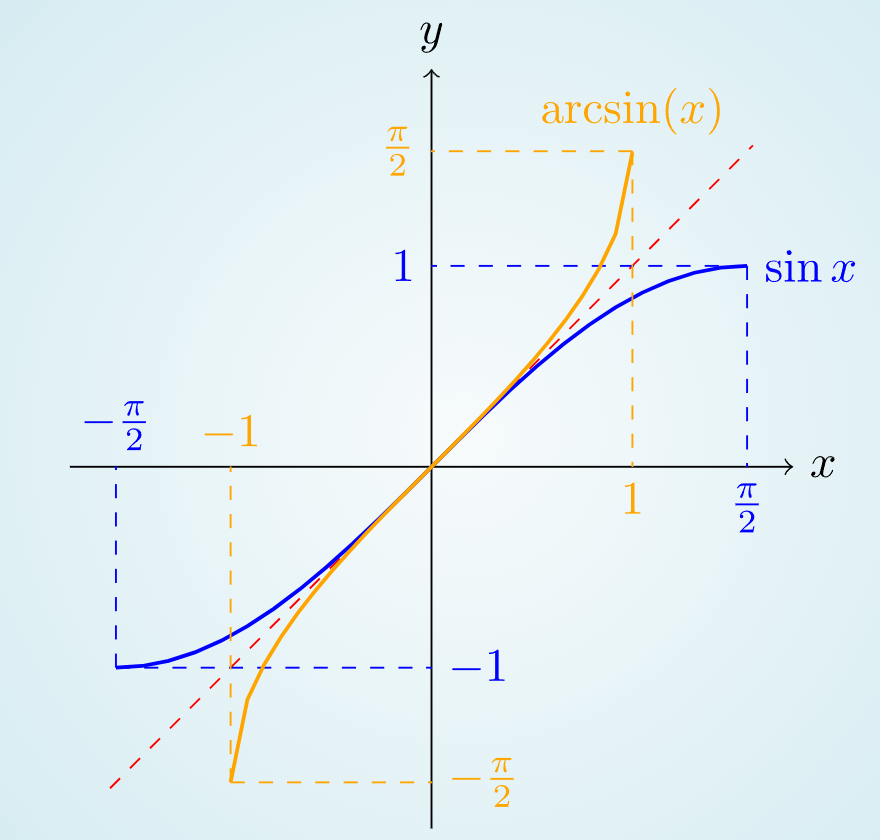
\includegraphics[width=0.4\textwidth]{"figure/Note/arcsinx.png"}}
	\subfigure[$\arccos(x)\ \&\ \cos (x)$]{
	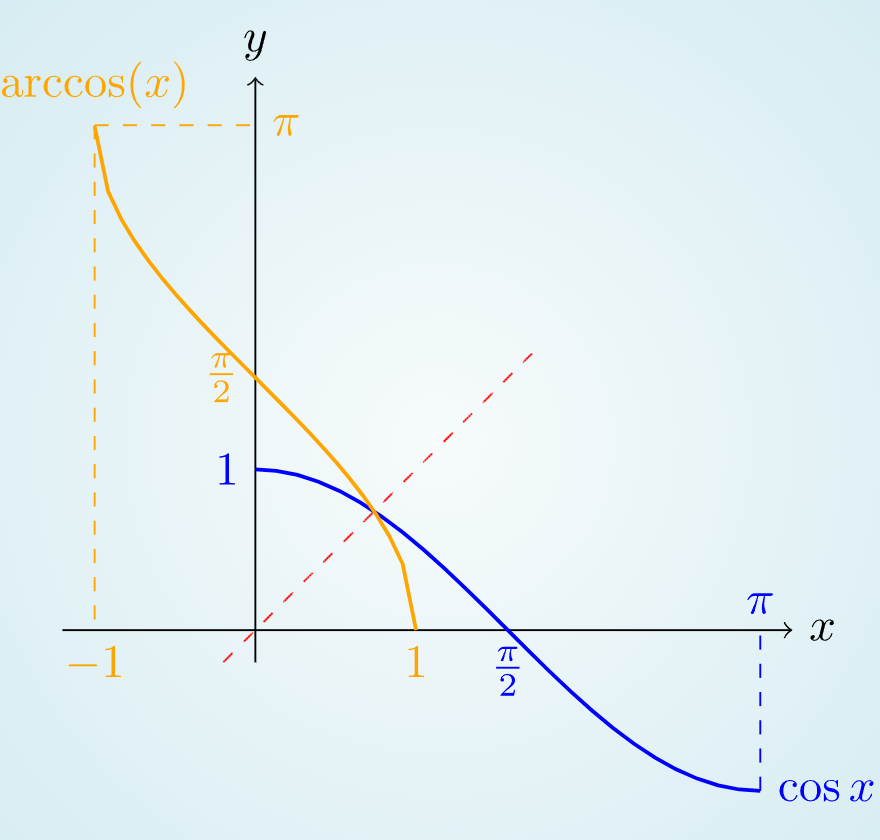
\includegraphics[width=0.4\textwidth]{"figure/Note/arccosx.png"}}
	\subfigure[$\arctan(x)\ \&\ \tan (x)$]{
	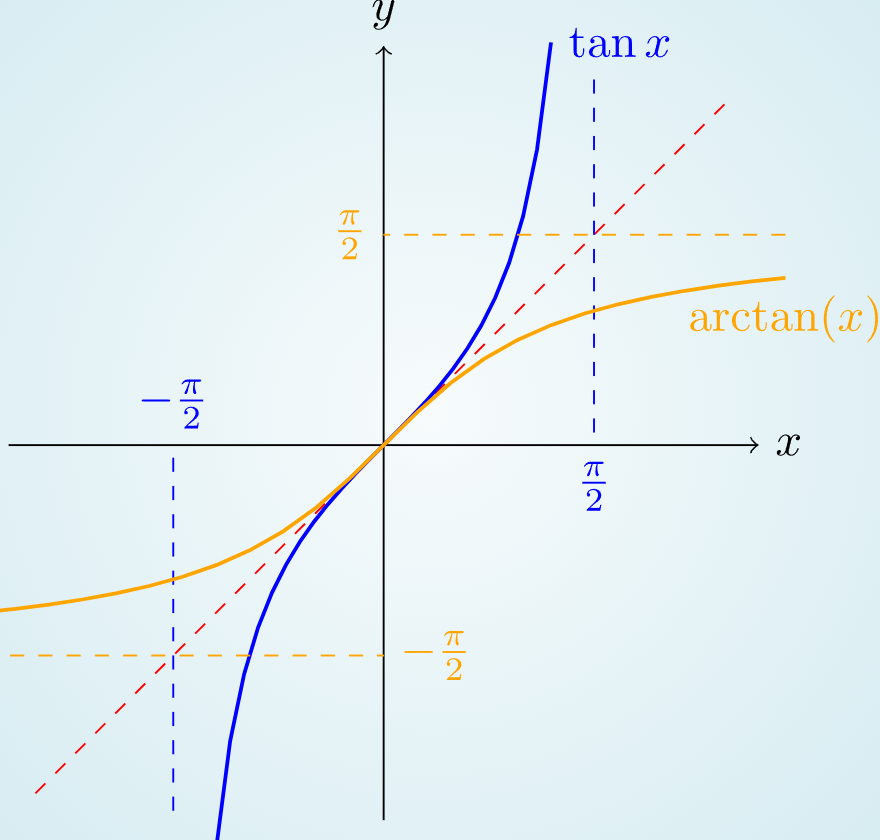
\includegraphics[width=0.4\textwidth]{"figure/Note/arctanx.png"}}
	\caption{反三角函数图像}
\end{figure}
\subsection{特殊函数}
\begin{definition}[特殊函数]
	\begin{enumerate}
		\item 阶乘函数: $$n!=n(n-1)(n-2)\cdots 2\cdot 1, (2n)!! = 2^{n}\cdot n!, 0! = 1$$
		\item 二项式系数: $$\binom{n}{k}=\dfrac{n!}{k!(n-k)!}, (a+b)^{n} = \sum\limits_{i = 0}^{n}\binom{n}{i}a^{i}b^{n-i}$$
		\item 绝对值函数: $$|x|=\begin{cases} x & x\geq 0 \\ -x & x<0 \end{cases}$$
		\item 符号函数: $$sgn(x)=\begin{cases} 1 & x>0 \\ 0 & x=0 \\ -1 & x<0 \end{cases}$$%
		\item 取整函数: $$f(x) = [x], x-1< [x] \leq x, \lim\limits_{x\to 0^{+}} = 0, \lim\limits_{x\to 0^{-}} =-1$$
		\item 分段函数: $$f(x)=\begin{cases} f_{1}(x) & x\in D_{1} \\ f_{2}(x) & x\in D_{2} \\ \cdots \end{cases}$$
		\item 黎曼函数:$$f(x)=\begin{cases} \dfrac{1}{q} & p,q\in \mathbb{Q}, x = \dfrac{p}{q}\in(0,1) \\ 0 & x\notin \mathbb{Q}, x=0,1 \end{cases}$$
		\item 狄利克雷函数: $$f(x)=\begin{cases} 1 & x\in \mathbb{Q} \\ 0 & x\notin \mathbb{Q} \end{cases}$$
	\end{enumerate}
\end{definition}


\begin{theorem}[平均值不等式 $a_{i} > 0$]
	平方平均值:
	$$Q_{n}=\sqrt{\dfrac{\sum\limits_{k=1}^{n}a_{k}^{2}}{n}}$$
	算术平均值:
	$$A_{n}=\dfrac{\sum\limits_{i=1}^{n}a_{i}}{n}$$
	几何平均值:
	$$G_{n}=\sqrt[n]{\prod\limits_{i=1}^{n}a_{i}}$$
	调和平均值:
	$$H_{n}=\dfrac{n}{\sum\limits_{i=1}^{k}\dfrac{1}{a_{i}}}$$
	平均值不等式:
	$$Q_{n}\geq A_{n}\geq G_{n}\geq H_{n}, a_{1} = a_{2} = \cdots = a_{n} \text{等号成立}$$
\end{theorem}

\begin{theorem}[柯西不等式]
	二维形式:
	$$(a^{2}+b^{2})(c^{2}+d^{2})\geq (ac+bd)^{2}, \text{当且仅当} ad =bc \text{时等号成立}$$
	$n$ 维形式:
	$$\left(\sum_{i=1}^{n}a_{i}b_{i}\right)^{2}\leq \left(\sum_{i=1}^{n}a_{i}^{2}\right)\left(\sum_{i=1}^{n}b_{i}^{2}\right),\text{当且仅当} \dfrac{a_{i}}{b_{i}}=c\text{时等号成立}$$
	$$\text{向量形式: } (\alpha,\beta)^{2}\leq (\alpha,\alpha)(\beta,\beta)$$
\end{theorem}
\begin{theorem}[重要不等式]
	\begin{enumerate}
		\item $\sin x < x < \tan x, x\in (0,\dfrac{\pi}{2})\qquad \qquad \arctan x < x < \arcsin x, x\in[0,1]$
		\item $\dfrac{2}{\pi}x < \sin x < x, x\in(0,\dfrac{\pi}{2})\qquad \qquad x < \tan x < \dfrac{4}{\pi}x , x\in(0,\dfrac{\pi}{4})$
		\item $e^{x} \geq x + 1,x\in\mathbb{R}\qquad \qquad x-1 \geq \ln x, x\in(0,+\infty)$
		\item $\dfrac{1}{1+x} < \ln (1+\dfrac{1}{x}) < \dfrac{1}{x}, x\in(0,+\infty)$
	\end{enumerate}
\end{theorem}

\begin{theorem}[重要公式]
	\begin{enumerate}
		\item $\dfrac{n}{(n+1)!} = \dfrac{1}{n!} - \dfrac{1}{(n+1)!}$
		\item $(a^{3}-b^{3}) = (a-b)(a^{2}+ab+b^{2})\qquad\qquad (a^{3}+b^{3}) = (a+b)(a^{2}-ab+b^{2})$
		\item $a^{n} - b^{n} = (a-b)(a^{n-1}-a^{n-2}b+\cdots -ab^{n-2}+b^{n-1})$
		\item $a^{n} + b^{n} = (a+b)(a^{n-1}-a^{n-1}b+\cdots -ab^{n-2} +b^{n-1}), n\in \{2k+1 | k\in \mathbb{N}\}$
	\end{enumerate}
\end{theorem}

\section{函数的表示方法}
\subsection{显式表达}
\begin{definition}[显示表达]
	$y = f(x)$ 的形式, 初等函数都是显性表达.
\end{definition}
\subsection{隐式表达}
\begin{definition}[隐式表达]
	$f(x,y) = 0$ 的形式, 一般不能用 $x$ 表示 $y$, 也不能用 $y$ 表示 $x$
\end{definition}
\subsection{极坐标}
\begin{definition}[极坐标]
	极坐标系是平面直角坐标系的一种推广, 它是由一个原点 $O$ 和一个射线 $Ox$ 组成的, 其中 $O$ 称为极点, $Ox$ 称为极轴, 任意一点 $P$ 到极点 $O$ 的距离 $r$ 叫做点 $P$ 的极径, 点 $P$ 到极轴的角 $\theta$ 叫做点 $P$ 的极角, 记为 $P(r,\theta)$
\end{definition}

\begin{definition}[重要极坐标方程]
	\begin{enumerate}
		\item 圆方程: $r = a, r = a\sin\theta, r = a\cos\theta$
		\item 心形线方程: $r = a(1\pm \cos\theta), r = a(1\pm \sin\theta)$
		\item 阿基米德螺线方程: $r = a\theta$
		\item 三叶玫瑰线方程: $r = a\sin 3\theta, r = a\cos 3\theta$
		\item 伯努利双扭线方程: $r^{2} = a^{2}\cos 2\theta, r^{2} = a^{2}\sin 2\theta$
	\end{enumerate}
\end{definition}
\subsection{参数方程}
\begin{definition}[参数方程]
	设 $x=x(t),y=y(t)$, 如果 $x,y$ 都是 $t$ 的函数, 那么称 $x=x(t),y=y(t)$ 为参数方程, $t$ 称为参数
\end{definition}
\begin{definition}[重要参数方程]
	\begin{enumerate}
		\item 摆线方程: $x = a(t-\sin t), y = a(1-\cos t)$
		\item 星形线方程: $x = a\cos^{3} t, y = a\sin^{3} t$
	\end{enumerate}
\end{definition}

\begin{anymark}[注]
	1. 关于双曲函数以及反双曲函数, 在 $\mathbf{def:}$ \ref{def: 双曲函数} 有详细介绍
	
	2. 有关极坐标和参数方程常见曲线的方程, 在 $\mathbf{def:}$ \ref{def: 常用曲线} 有详细介绍 
\end{anymark}




\chapterimage{chap2.jpg}

\chapter{数列极限}
\begin{introduction}
	\item 数列极限定义和性质
	\item 归结原理
	\item 夹逼准则
	\item 单调有界准则
\end{introduction}
\section{数列极限}
\begin{definition}[数列极限]
	设 $x_{n}$ 是 一数列, 若存在常数 $a$, $\forall \epsilon>0$, $\exists N_{0}>0$, 当 $n>N_{0}$ 时, $|x_{n}-a|<\epsilon$ 恒成立, 常数 $a$ 是数列 $\{x_{n}\}$ 的极限或者说数列 $\{x_{n}\}$ 趋近于 $a$
\end{definition}


\begin{property}[唯一性]
	若极限存在, 则极限唯一
\end{property}

\begin{property}[有界性]
	若数列 $\{x_{n}\}$ 的极限 $a$ 存在, 则数列 $\{x_{n}\}$ 有界
\end{property}

\begin{property}[保号性]
	若数列 $\{x_{n}\}$ 的极限 $a>0(a<0)$, 则存在正整数 $N_{0}$, 当 $n>N_{0}$ 时, $x_{n}>0(x_{n}<0)$, 取 $\epsilon = \pm a$ 即可
\end{property}
\begin{anymark}[注]
	1. 若数列的任意子列发散, 数列极限不存在

	2. 若数列的任意两个子列极限存在但不相等, 数列极限不存在
\end{anymark}
\begin{corollary}[数列极限]
	\begin{itemize}
		\item 如果数列从某项起有 $x_{n}\geq 0$ 且 $\lim\limits_{n\to\infty}x_{n} = a$, 则 $a\geq 0$
		\item 如果 $\lim\limits_{n\to\infty} x_{n} = A$, 则 $\lim\limits_{n\to\infty} |x_{n}| = |A|$
		\item $\lim\limits_{n\rightarrow +\infty}x_{n}=a\to \begin{cases} \lim\limits_{n\rightarrow +\infty}\dfrac{x_{n+1}}{x_{n}}=1, & a\neq 0\\ \lim\limits_{n\rightarrow +\infty}\dfrac{x_{n+1}}{x_{n}} \text{不一定存在}, & a=0  \end{cases}$
		\item $\lim\limits_{n\rightarrow +\infty}\dfrac{x_{n+1}}{x_{n}}=a\to \begin{cases} \lim\limits_{n\rightarrow +\infty}x_{n}=\infty,& |a|>1  \\ \lim\limits_{n\rightarrow +\infty}x_{n}=0,&|a|<1\\  \lim\limits_{n\rightarrow +\infty}x_{n}\text{不确定},&|a|=1 \end{cases}$
		\item $\lim\limits_{n\rightarrow +\infty}\dfrac{x_{n+1}}{x_{n}}\text{存在且}x_{n}>0\to \lim\limits_{n\rightarrow +\infty}\sqrt[n]{x_{n}}=\lim\limits_{n\rightarrow +\infty}\dfrac{x_{n+1}}{x_{n}}$
	\end{itemize}
\end{corollary}

\section{数列极限计算}
\subsection{定义法}
\begin{definition}[极限的四则运算]
	$$\lim\limits_{n\to \infty}x_{n}=a,\lim\limits_{n\to \infty}y_{n}=b$$
	\begin{enumerate}
		\item $\lim\limits_{n\to \infty}(x_{n}\pm y_{n}) = a\pm b$
		\item $\lim\limits_{n\to \infty}(x_{n}\cdot y_{n}) = a\cdot b$
		\item $\lim\limits_{n\to \infty}\dfrac{x_{n}}{y_{n}} = \dfrac{a}{b}, b\neq 0$
	\end{enumerate}

\end{definition}
\subsection{归结原理}
\begin{definition}[归结原理]
	设函数 $f(x)$ 在去心邻域 $\mathring{U}(a,\delta)$ 上有定义, 那么 $\lim\limits_{x\to a}f(x) = l$ 的充分必要条件是: 对与一切序列 $\{x_{n}\}_{n=1}^{\infty}\subset \mathring{U}(a,\delta)$, 只要 $\lim\limits_{n\to\infty}x_{n}=a$, 就有 $\lim\limits_{n\to\infty}f(x_{n})=l$
\end{definition}
\subsection{夹逼准则}
\begin{definition}[夹逼准则]
	设数列 $\{x_{n}\}$, $\{y_{n}\}$, $\{z_{n}\}$ 满足 $x_{n}\leq y_{n}\leq z_{n}$, $\lim\limits_{n\to\infty}x_{n}=\lim\limits_{n\to\infty}z_{n}=a$, 则 $\lim\limits_{n\to\infty}y_{n}=a$, 条件可变为 $n>N_{0}$ 时, $x_{n}\leq y_{n}\leq z_{n}$(有限无关性)
\end{definition}

\begin{corollary}[夹逼准则]
	$\lim\limits_{n\rightarrow +\infty}\sqrt[n]{u_{1}^{n}+u_{2}^{n}+u_{3}^{n}+\cdots+u_{m}^{n}}=\max\{ u_{1},u_{2},\cdots,u_{m}\}$
	\begin{anymark}[证明]
		$$[\max\{ u_{1},u_{2},\cdots,u_{m}\}]^{n}\leq u_{1}^{n}+u_{2}^{n}+u_{3}^{n}+\cdots+u_{m}^{n}\leq m[\cdot\max\{ u_{1},u_{2},\cdots,u_{m}\}]^{n}$$
	
		我们将$[\max\{ u_{1},u_{2},\cdots,u_{m}\}]^{n}$记作$a$,$m\cdot[\max\{ u_{1},u_{2},\cdots,u_{m}\}]^{n}$记作$b$,我们利用夹逼准则:

	$$\lim\limits_{n\rightarrow +\infty}\sqrt[n]{a}=\lim\limits_{n\rightarrow +\infty}\sqrt[n]{b}=\text{max}\{ u_{1},u_{2},\cdots,u_{m}\}$$
	\end{anymark}
\end{corollary}

\subsection{单调有界准则}
\begin{definition}[单调有界准则]
	单调有界数列必有极限, 详细证明见 $\mathbf{the:}$ \ref{the: 柯西收敛准则}.
\end{definition}
\section{Exercise}
\begin{proposition}
	设$x_{1}=a\geq 0$,$y_{1}=b\geq 0$,$a\leq b$,$x_{n+1}=\sqrt{x_{n}y_{n}},y_{n+1}=\dfrac{x_{n}+y_{n}}{2}(n=1,2,\cdots)$,证明:
	$\lim\limits_{n\rightarrow +\infty}x_{n}=\lim\limits_{n\rightarrow +\infty}y_{n}$
\end{proposition}
\begin{solution}
	
	$x_{1}=a\geq 0$,$y_{1}=b\geq 0$,$x_{n+1}=\sqrt{x_{n}y_{n}},y_{n+1}=\dfrac{x_{n}+y_{n}}{2}$
	
	数学归纳法:  
	$$x_{n}\geq 0, y_{n}\geq 0$$
	
	基本不等式:  
	$$\dfrac{x_{n}+y_{n}}{2}\geq \sqrt{x_{n}y_{n}}\Rightarrow y_{n+1}\geq x_{n+1}$$
	
	$$
	\begin{cases}
		x_{n+1}=\sqrt{x_{n}y_{n}}\geq \sqrt{x_{n}x_{n}} = x_{n}\\
		y_{n+1}=\dfrac{x_{n}+y_{n}}{2}\leq \dfrac{y_{n}+y_{n}}{2} = y_{n}
	\end{cases}
	$$
	
	$\{x_{n}\}$ 单调递增,$\{y_{n}\}$ 单调递减, $x_{1}\leq x_{n}\leq y_{n}\leq y_{1}$
	
	$\{x_{n}\},\{y_{n}\}$ 单调且有界, 数列 $\{x_{n}\},\{y_{n}\}$ 均有极限 
	$$\begin{cases}
		\lim\limits_{n\rightarrow +\infty}x_{n} = a\\
		\lim\limits_{n\rightarrow +\infty}y_{n} = b
	\end{cases} \Rightarrow 
	\begin{cases}
		a = \sqrt{ab}\\
		b = \dfrac{a+b}{2}
	\end{cases}\Rightarrow a=b$$
	
	综上所述, $\lim\limits_{n\rightarrow +\infty}x_{n}=\lim\limits_{n\rightarrow +\infty}y_{n}$
\end{solution}

\begin{proposition}
	设数列 $\{a_{n}\}$ 满足 $\lim\limits_{n\rightarrow+\infty}\dfrac{a_{n+1}}{a_{n}}=q$, 且 $|q|<1$, 证明: $\lim\limits_{n\rightarrow+\infty}a_{n}=0$
\end{proposition}
\begin{solution}
	
	考虑数列 $\{|a_{n}|\}$:

	$$\begin{cases}
		\lim\limits_{n\rightarrow+\infty}\dfrac{a_{n+1}}{a_{n}} = q\\
		|\dfrac{a_{n+1}}{a_{n}}-q| \geq \big||\dfrac{a_{n+1}}{a_{n}}|-|q|\big| 
	\end{cases}\Rightarrow
	\begin{cases}
		\forall \varepsilon > 0, \exists M > 0, n > M, |\dfrac{a_{n+1}}{a_{n}}-q| < \varepsilon \\
		\forall \varepsilon > 0, \exists M > 0, n > M, \big||\dfrac{a_{n+1}}{a_{n}}|-|q|\big| < \varepsilon
	\end{cases}
	\Rightarrow \lim\limits_{n\rightarrow+\infty}\big|\dfrac{a_{n+1}}{a_{n}}\big| = |q|$$
	
	取 $\varepsilon > 0 ,\varepsilon + |q| < 1$
	$$\exists N > 0, n > N, \big|\dfrac{a_{n+1}}{a_{n}}-|q|\big| < \varepsilon \Rightarrow n > N, \big| \dfrac{a_{n+1}}{a_{n}}\big| < \varepsilon + |q| < 1$$
	
	$$\begin{cases}
		|a_{n}| \geq 0\\
		|a_{n}| = \big|\dfrac{a_{n}}{a_{n-1}}\big|\cdots\big|\dfrac{a_{N+2}}{a_{N+1}}\big|\cdot|a_{N+1}| <  (|q|+\varepsilon)^{n-N-1}\cdot |a_{N+1}|
	\end{cases}$$

	夹逼准则:
	$$
	\begin{cases} 
		\lim\limits_{n\to +\infty} 0 = 0\\
		\lim\limits_{n\to +\infty} (|q|+\varepsilon)^{n-N-1}\cdot |a_{N+1}| = 0
	\end{cases}\Rightarrow
	\begin{cases}
		\lim\limits_{n\to +\infty} |a_{n}| = 0\\
		\forall \varepsilon > 0, \exists N > 0, n > N, |a_{n}| < \varepsilon
	\end{cases}
	\Rightarrow \lim\limits_{n\to +\infty} a_{n} = 0 
	$$
	
	综上所述, $\lim\limits_{n\rightarrow+\infty}a_{n}=0$
\end{solution}

\begin{proposition}
	设$f_{n}(x)=1-(1-\cos x)^n(n=1,2,\cdots)$

(1). 证明:  方程$f_{n}(x)=\dfrac{1}{2}$在$(0,\dfrac{\pi}{2})$内有且只有一个实数根$x_{n}$

(2). 设$x_{n}\in(0,\dfrac{\pi}{2})$,满足$f_{n}(x)=\dfrac{1}{2}$,证明:  $$\arccos \dfrac{1}{n}<x_{n}<\dfrac{\pi}{2},\text{且}\lim\limits_{n\rightarrow +\infty}x_{n}=\dfrac{\pi}{2}$$
\end{proposition}
\begin{solution}
	
	构造辅助函数: $G_{n}(x)=\dfrac{1}{2}-(1-\cos x)^{n}$
	
	(1). $$G_{n}'(x)=-n\sin x(1-\cos x)^{n-1}$$
	
	$x\in(0,\dfrac{\pi}{2})$, $G_{n}'(x)<0$, $G_{n}(x)$ 在 $(0,\dfrac{\pi}{2})$ 单调递减
	
	$$G_{n}(0)=\dfrac{1}{2}>0  G_{n}(\dfrac{\pi}{2})=-\dfrac{\pi}{2}<0$$
	
	零点定理: $\exists!\ x_{n}\in(0,\dfrac{\pi}{2}),\ s.t.\ G_{n}(x_{n})=0$
	
	(2). 
	$$\begin{cases}
		G_{n}(\arccos\dfrac{1}{n}) = \dfrac{1}{2}-(1-\dfrac{1}{n})^{n} \\
		G_{n}(\dfrac{\pi}{2}) = -\dfrac{1}{2} < 0
	\end{cases}$$
	
    构造辅助函数: $h(x) = \dfrac{1}{2} - e^{x\ln(1-\frac{1}{x})},x\geq 2$
	
	$$\begin{cases}
		p(x) = \ln(1-\frac{1}{x}) + \dfrac{1}{x-1}, x\geq 2\\
		\lim\limits_{x\to +\infty} p(x) = 0\\
		p'(x) = \dfrac{-1}{x(x-1)^{2}} < 0  
	\end{cases}\Rightarrow 
	h'(x) = -e^{x\ln(1-\frac{1}{x})}\left[\ln(1-\frac{1}{x})+\dfrac{1}{x-1}\right] < 0$$
	
	$G_{n}(\arccos\dfrac{1}{n})$ 单调递减, 且 $\lim\limits_{n\rightarrow+\infty}G_{n}(\arccos\dfrac{1}{n})=\dfrac{1}{2}-\dfrac{1}{e}>0$
	零点定理: 
	$$\exists! x_{n}\in (\arccos \dfrac{1}{n}, \dfrac{\pi}{2}),\ s.t.\ f(x_{n}) = \dfrac{1}{2}$$
	
	夹逼定理:  
	$$\begin{cases}
		\lim\limits_{n\rightarrow  +\infty}\arccos \dfrac{1}{n}=\dfrac{\pi}{2}\\
		\lim\limits_{n\rightarrow  +\infty}\dfrac{\pi}{2}=\dfrac{\pi}{2}
	\end{cases}
	\Rightarrow \lim\limits_{n\rightarrow +\infty}x_{n}=\dfrac{\pi}{2}$$
	
\end{solution}

\begin{proposition}
	设$x_{1}>0$,数列$\{x_{n}\}$满足$x_{n+1}=\ln(e^{x_{n}}-1)-\ln x_{n}$,证明:  $\lim\limits_{n\rightarrow +\infty}x_{n}$存在并求其值
\end{proposition}
\begin{solution}
	
	$$x_{n+1}=\ln(e^{x_{n}}-1)-\ln x_{n} \Rightarrow e^{x_{n+1}}=\dfrac{e^{x_{n}}-1}{x_{n}}$$
	
	构造辅助函数: $f(x)=e^x-x-1, f'(x)=e^{x}-1$
	$$\begin{cases}
		x > 0, f'(x) > 0\\
		f(x) > f(0) = 0\\
		\dfrac{e^{x}-1}{x} > 1
	\end{cases}\Rightarrow 
	\begin{cases}
		x_{1} > 0\\
		x_{2} = \ln(\dfrac{e^{x_{1}}-1}{x_{1}}) > 0
	\end{cases}
	$$
	
	数学归纳法: $x_{n}>0$, 数列 $\{ x_{n}\}$ 有下界
	
	拉格朗日中值定理:  
	$$e^{x_{n+1}}=\dfrac{e^{x_{n}}-1}{x_{n}}=e^{\xi}, \xi\in(0,x_{n})\Rightarrow x_{n+1} = \xi < x_{n}$$
	
	数列 $\{x_{n}\}$ 单调递减且有下界, 单调有界准则: 数列 $\{x_{n}\}$ 极限必定存在
	
	不妨设 $\lim\limits_{n\rightarrow +\infty}x_{n}=a$ :  
	$$e^{a}=\dfrac{e^a-1}{a}\Rightarrow a=0$$
	
	综上所述,数列$\{x_{n}\}$极限存在,其值为$0$
\end{solution}
\begin{proposition}
	设 $f(x)$ 在 $[a,b]$ 上可导, 且 $|f'(x)|<1$, 当 $x\in[a,b]$ 时,有 $a<f(x)<b$,$F(x)=\dfrac{x+f(x)}{2}$,证明:  

(1). $\exists!\ x^{*}\in(a,b),\ s.t.\ F(x^{*})=x^{*}$

(2). 对 $x_{0}\in[a,b]$, 数列 $\{x_{n}\}$ 满足 $x_{n+1}=F(x_{n})(n=0,1,2,\cdots)$, 有 $\lim\limits_{n\rightarrow+\infty}x_{n}=x^{*}$

\end{proposition}
\begin{solution}
	
	(1). 
	
	构造辅助函数: $G(x) = F(x)-x = \dfrac{f(x)-x}{2}$, $G'(x)=\dfrac{f'(x)-1}{2}$
	
	$$|f'(x)|<1\Rightarrow G'(x)<0\Rightarrow G(x)\text{单调递减}$$

	$$\begin{cases}
		G(a) = \frac{f(a)-a}{2}>0\\
		G(b) = \frac{f(b)-b}{2}<0
	\end{cases} \Rightarrow G(a)G(b)<0$$
	
	零点定理: 
	$$\exists!\ x^{*}\in(a,b),\ s.t.\ G(x^{*})=0\Rightarrow \exists!\ x^{*}\in(a,b),\ s.t.\ F(x^{*})=x^{*}$$
	
	(2). 

	$$F'(x)=\dfrac{1+f'(x)}{2}\geq 0\Rightarrow F(x)\text{单调递增}$$
	
	(i). $x_{0}=x^{*}$,$x_{n}=x^{*}$, $\lim\limits_{n\rightarrow +\infty}x_{n}=x^{*}$
	
	(ii). $x_{0}>x^{*}$, $G(x^{*})>G(x_{0})\Rightarrow F(x_{0})<x_{0}\Rightarrow x_{1}<x_{0}$
	\begin{enumerate}
		\item 当 $n=1$ 时, $x_{1}<x_{0}$
		\item 假设当 $n=k(k\geq 1)$ 时, $x_{k}<x_{k-1}$ 成立
		\item 当 $n=k+1$ 时, $F(x_{k})<F(x_{k-1})\Rightarrow x_{k+1}<x_{k}$
	\end{enumerate}
	$$\begin{cases}
		x_{n+1}=\frac{x_{n}+f(x_{n})}{2} \\
		x_{1}\in [a,b] \\
		f(x_{n})\in (a,b)\\
	\end{cases}\Rightarrow x_{n}\in [a,b]$$
	
	数列 $\{x_{n}\}$ 单调递减且有下界,极限必定存在
	
	不妨设 $\lim\limits_{n\to +\infty}x_{n} = A$
	
	$$A=\dfrac{A+f(A)}{2}\Rightarrow F(A)=A\Rightarrow A=x^{*}$$
	
	(iii). $x_{0}<x^{*}$, $G(x^{*})<G(x_{0})\Rightarrow F(x_{0})>x_{0}\Rightarrow x_{1}>x_{0}$
	\begin{enumerate}
		\item 当 $n=1$ 时, $x_{1}>x_{0}$
		\item 假设当 $n=k(k\geq 1)$ 时, $x_{k}>x_{k-1}$ 成立
		\item 当 $n=k+1$ 时, $F(x_{k})>F(x_{k-1})\Rightarrow x_{k+1}>x_{k}$
	\end{enumerate}
	$$\begin{cases}
		x_{n+1}=\frac{x_{n}+f(x_{n})}{2} \\
		x_{1}\in [a,b] \\
		f(x_{n})\in (a,b)\\
	\end{cases}\Rightarrow x_{n}\in [a,b]$$
	
	数列 $\{x_{n}\}$ 单调递增且有上界,极限必定存在
	
	不妨设 $\lim\limits_{n\to +\infty}x_{n} = A$
	
	$$A=\dfrac{A+f(A)}{2}\Rightarrow F(A)=A\Rightarrow A=x^{*}$$
	
	综上所述, $\lim\limits_{n\rightarrow+\infty}x_{n}=x^{*}$
\end{solution}
\begin{proposition}
(1).设$f(x)$是$[0,+\infty)$上单调减少且非负的连续函数,证明:  $$f(k+1)\leq \int_{k}^{k+1}f(x)dx\leq f(k),\ k=1,2,\cdots$$

(2). 证明:  $\ln(1+n)\leq 1+\dfrac{1}{2}+\cdots+\dfrac{1}{n}\leq 1+\ln n$,求极限$\lim\limits_{n\rightarrow+\infty}\dfrac{1+\dfrac{1}{2}+\cdots+\dfrac{1}{n}}{\ln n}$

\end{proposition}
\begin{solution}
	
	(1). 
	
	$f(x)$单调减少且非负:  
	$$0\leq f(k+1)\leq f(x)\leq f(k),\ x\in[k,k+1]$$
	
	不等式在 $[k,k+1]$ 上同时求定积分:  
	$$\int_{k}^{k+1}f(k+1)dx\leq \int_{k}^{k+1}f(x)dx\leq \int_{k}^{k+1}f(k)dx\Rightarrow f(k+1)\leq \int_{k}^{k+1}f(x)dx\leq f(k)$$
	
	(2). 
	
	构造辅助函数 $f(x)=\dfrac{1}{x}$, $f(x)$ 在 $(0,+\infty)$ 上单调递减且非负:  
	$$\begin{cases}
		\displaystyle{\dfrac{1}{2}\leq \int_{1}^{2}\dfrac{1}{x}dx\leq 1} \\
		\displaystyle{\dfrac{1}{3}\leq \int_{2}^{3}\dfrac{1}{x}dx\leq \dfrac{1}{2}} \\
		\cdots\\
		\displaystyle{\dfrac{1}{n}\leq \int_{n-1}^{n}\dfrac{1}{x}dx\leq \dfrac{1}{n-1}}\\
		\displaystyle{\dfrac{1}{n+1}\leq \int_{n}^{n+1}\dfrac{1}{x}dx\leq \dfrac{1}{n}}
	\end{cases} \Rightarrow
	\begin{cases}
		\displaystyle{\sum\limits_{k=1}^{n}\dfrac{1}{k+1}\leq \int_{1}^{n+1}\dfrac{1}{x}=\ln(1+n)\leq \sum\limits_{k=1}^{n}\dfrac{1}{k}}\\
		\displaystyle{\sum\limits_{k=1}^{n-1}\dfrac{1}{k+1}\leq \int_{1}^{n}\dfrac{1}{x}=\ln n}\\
		\displaystyle{\sum\limits_{k=1}^{n}\dfrac{1}{k}=1+\sum\limits_{k=1}^{n-1}\dfrac{1}{k+1}\leq 1+\ln n}
	\end{cases}$$
	
	$$\ln(1+n)\leq \sum\limits_{k=1}^{n}\dfrac{1}{k}\leq 1+\ln n$$

	夹逼定理:  
	$$\begin{cases}
		\lim\limits_{n\rightarrow +\infty}\dfrac{\ln(1+n)}{\ln n} = 1\\
		\lim\limits_{n\rightarrow +\infty}\dfrac{1+\ln n}{\ln n} = 1
	\end{cases}\Rightarrow 
	\lim\limits_{n\rightarrow +\infty}\dfrac{1+\dfrac{1}{2}+\cdots+\dfrac{1}{n}}{\ln n}=1$$
\end{solution}

\begin{proposition}
	设 $f(x)$ 在 $(a,b)$ 内连续, 且 $\lim\limits_{x\rightarrow a^{+}}f(x)=\lim\limits_{x\rightarrow b^{-}}f(x)=-\infty$, 证明: $f(x)$在$(a,b)$ 内有最大值
\end{proposition}
\begin{solution}
	
	取 $M=f(\dfrac{a+b}{2})$
	
	极限定义:  
	$$\begin{cases}
		\exists a < c < \dfrac{a+b}{2},x\in(a,c),\ s.t.\ f(x)\leq f(\dfrac{a+b}{2})\\
		\exists \dfrac{a+b}{2} < d < b,x\in(d,b),\ s.t.\ f(x)\leq f(\dfrac{a+b}{2})
	\end{cases}$$
	
	$$\begin{cases}
		\exists \xi\in [c,d], \forall x\in [c,d], f(\xi)\geq f(x)\\
		f(\xi) \geq f(\dfrac{a+b}{2})\\
		x\in (a,c], f(x) < f(\dfrac{a+b}{2}) \leq f(\xi)\\
		x\in [d,b), f(x) < f(\dfrac{a+b}{2}) \leq f(\xi)
	\end{cases}$$
	
	综上所述, $f(x)$ 在区间 $(a,b)$ 内有最大值 $f(\xi)$
\end{solution}

\begin{lemma}[不单调数列极限]
\begin{enumerate}
	\item 压缩映射原理: 从定义出发, 证明: $|x_{n}-a|$ 极限为 $0$
	\item 柯西列: $\sum\limits_{n=1}^{+\infty}(x_{n+1}-x_{n})$, 证明这个级数收敛即可证明出数列 $\{x_{n}\}$ 极限存在
	\item 奇数项和偶数项极限存在且相等: $\lim\limits_{n\to\infty}x_{2n}=\lim\limits_{n\to\infty}x_{2n-1}=A$
\end{enumerate} 
\end{lemma}

\begin{proposition}
	设 $2x_{1}=1,2x_{n+1}=1-x_{n}^2$, 证明数列 $\{x_{n}\}$ 收敛,
	并求极限 $\lim\limits_{n\rightarrow +\infty}x_{n}$
\end{proposition}
\begin{solution}
	
	$$x_{1} = \dfrac{1}{2}, x_{2} = \dfrac{3}{8}, x_{3} = \dfrac{55}{128}\Rightarrow x_{1} > x_{3} > x_{2}$$
	
	数列$\{x_{n}\}$不单调, 不能使用单调有界准则来判断

	$$\begin{cases} 
		x_{n+1} = \dfrac{1-x_{n}^{2}}{2}\\
		x_{1} = \dfrac{1}{2}\in (0,1)\\
		x\in(0,1),1-x^{2}\in(0,1)
	\end{cases}\Rightarrow x_{n}\in (0,\dfrac{1}{2})$$
	\begin{anymark}[压缩映射原理]

		不妨设 $\lim\limits_{n\rightarrow\infty}x_{n}=a(a>0)$, 对 $2x_{n+1}=1-x_{n}^2$ 两边同时取极限: 
	    
		$$2a=1-a^2\Rightarrow 
		\begin{cases}
			a=\dfrac{1-a^2}{2} \\
			a=\sqrt{2}-1
		\end{cases}$$
			
		\begin{eqnarray*}
			|x_{n+1}-a| &  =   & \big|\dfrac{1-x_{n}^2}{2}-\dfrac{1-a^2}{2}\big|\\
					    &  =   & \big|\dfrac{x_{n}^{2}-a^2}{2}\big| = \dfrac{(x_{n}+a)}{2}|x_{n}-a|\\
					    & \leq & \dfrac{2\sqrt{2}-1}{4}|x_{n-1}-a|\\
					    & \leq & \cdots\\
					    & \leq & (\dfrac{2\sqrt{2}-1}{4})^{n-1}|x_{1}-a|
		\end{eqnarray*}
		
		$$\lim\limits_{n\to \infty} 0 = \lim\limits_{n\to \infty}(\dfrac{2\sqrt{2}-1}{4})^{n-1}=0$$
		
		夹逼定理: $\lim\limits_{n\to \infty}|x_{n}-a|=0 \Rightarrow \lim\limits_{n\rightarrow +\infty}x_{n} = a =\sqrt{2}-1$
	\end{anymark}
	\begin{anymark}[柯西列]

		构造无穷级数: $\sum\limits_{n=1}^{+\infty}(x_{n+1}-x_{n})$
		
		\begin{eqnarray*}
			|x_{n+1}-x_{n}| &   =  & \big|\dfrac{x_{n}^2-x_{n-1}^2}{2}\big| = \dfrac{x_{n}+x_{n-1}}{2}|x_{n}-x_{n-1}|\\
					  		& \leq & \dfrac{1}{2}|x_{n}-x_{n-1}|\\
					  		& \leq & \cdots\\
					  		& \leq & \dfrac{1}{2^{n-1}}|x_{2}-x_{1}|
		\end{eqnarray*}
		
		级数 $\sum\limits_{n=1}^{+\infty}\dfrac{1}{2^{n-1}}$ 收敛

		比较判别法: 
		$$\sum\limits_{n=1}^{+\infty}|x_{n+1}-x_{n}|\text{收敛}\Rightarrow \sum\limits_{n=1}^{+\infty}(x_{n+1}-x_{n}) \text{收敛}$$ 
		
		$$\begin{cases}
			\lim\limits_{n\to +\infty}\sum\limits_{k=1}^{n}(x_{k+1}-x_{k}) = A\\
			\lim\limits_{n\to +\infty}x_{n+1} - x_{1} =A
		\end{cases}\Rightarrow 
		\begin{cases}
			\lim\limits_{n\to +\infty}x_{n} = a\\
			2a = 1-a^{2}\\
			a > 0
		\end{cases}\Rightarrow a = \sqrt{2} -1$$
	\end{anymark}
\end{solution}

\begin{proposition}
	设 $x_{1}=1,x_{n}=1+\dfrac{1}{1+x_{n-1}},(n=1,2,\cdots)$,证明极限 $\lim\limits_{n\rightarrow\infty}x_{n}$ 存在并求出此极限
\end{proposition}
\begin{solution}
	
	$$ x_{1}=1,x_{2}=\dfrac{3}{2},x_{3}=\dfrac{7}{5},x_{4}=\dfrac{17}{12}\Rightarrow 
	\begin{cases}
		x_{1}<x_{3} \\
		x_{2}>x_{4} \\
		x_{n} > 0\\
		x_{n}\in (1,2)
	\end{cases}$$
	\begin{enumerate}
		\item 当 $n = 1$, $x_{1} < x_{3}, x_{2} > x_{4}$
		\item 假设 $n = k$ 时, $x_{2k-1} < x_{2k+1}, x_{2k} > x_{2k+2}$
		\item 当 $n = k+1$ 时:
		$$\begin{cases}
			x_{2k+3}=1+\dfrac{1}{1+x_{2k+2}}>1+\dfrac{1}{1+x_{2k}}=x_{2k+1} \\
			x_{2k+4}=1+\dfrac{1}{1+x_{2k+3}}<1+\dfrac{1}{1+x_{2k+1}}=x_{2k+2}
		\end{cases}$$
	\end{enumerate}

	$\{x_{2k-1}\}$ 单调递增且有上界,$\{x_{2k}\}$ 单调递减且有下界
	
	单调有界准则:
	$$\begin{cases}
		\lim\limits_{n\to\infty}x_{2n} = A(A>0)\\
		\lim\limits_{n\to\infty}x_{2n-1}=B(B>0)
	\end{cases}\Rightarrow 
	\begin{cases}
		A=1+\dfrac{1}{1+B}\\
		B=1+\dfrac{1}{1+A}
	\end{cases}\Rightarrow A=B=\sqrt{2}$$
\end{solution}

\begin{proposition}
	设$x_{1}=1,2x_{n+1}=x_{n}+\sqrt{x_{n}^2+\dfrac{1}{n^2}},(n=1,2,\cdots)$,证明极限数列$\{x_{n}\}$收敛.
\end{proposition}
\begin{solution}

	$$\begin{cases}
		x_{1} = 1 \\ 
		2x_{n+1} = x_{n} + \sqrt{x_{n}^{2}+\dfrac{1}{n^{2}}}
	\end{cases}\Rightarrow
	\begin{cases}
		x_{n+1} > x_{n} \\
		x_{n} \geq 1
	\end{cases} $$

	令 $$\begin{cases}
		a = \sqrt{x_{n}^{2}+\frac{1}{n^{2}}}\\
		b = x_{n}
	\end{cases}\Rightarrow
	\begin{cases}
		a^{2} -b^{2} = \dfrac{1}{n^{2}}\\
		a + b > 2
	\end{cases}$$
	\begin{eqnarray*}
		x_{n+1} - x_{n} & = & \dfrac{\sqrt{x_{n}^{2}+\frac{1}{n^{2}}}-x_{n}}{2} \\
						& = & \dfrac{a-b}{2}\\
						& = & \dfrac{a^{2}-b^{2}}{2(a+b)}\\
						& < & \dfrac{1}{4n^{2}}
	\end{eqnarray*}

	$$\sum\limits_{n=1}^{+\infty}(x_{n+1}-x_{n}) < \sum\limits_{n=1}^{+\infty}\dfrac{1}{4n^{2}}$$

	级数 $\sum\limits_{n=1}^{+\infty}\dfrac{1}{4n^{2}}$ 收敛

	比较判别法:
	$$\sum\limits_{n=1}^{+\infty}(x_{n+1}-x_{n})\text{收敛}\Rightarrow \lim\limits_{n\to +\infty}x_{n+1} - x_{1} = A$$
	
	综上所述, 极限 $\lim\limits_{n\rightarrow\infty}x_{n}$ 存在
\end{solution}

\begin{proposition}
	设 $x_{0}=1,x_{n+1}=\dfrac{1}{x_{n}^3+4},(n=0,1,2,\cdots)$, 证明极限 $\lim\limits_{n\rightarrow\infty}x_{n}$存在并求出此极限
\end{proposition}
\begin{solution}
	
	$$\begin{cases}
		x_{0} = 1\\
		x_{n+1} = \dfrac{1}{x_{n}^{3}+4}
	\end{cases} \Rightarrow x_{n}\in(0,1)$$
	\begin{eqnarray*}
		|x_{n+1}-x_{n}| & = & \big|\dfrac{1}{x_{n}^3+4}-\dfrac{1}{x_{n-1}^3+4}\big| \\
						& = & \dfrac{|x_{n}^{3}-x_{n-1}^{3}|}{(x_{n}^3+4)(x_{n-1}^3+4)} \\
						& = & \dfrac{|x_{n}^{2}+x_{n-1}^{2}+x_{n}x_{n-1}|}{(x_{n}^3+4)(x_{n-1}^3+4)}|x_{n}-x_{n-1}| \\
						& < & \dfrac{3}{16}|x_{n}-x_{n-1}|\\
						& < & \cdots\\
						& < & (\dfrac{3}{16})^{n}|x_{1}-x_{0}|
	\end{eqnarray*}
	$$\sum\limits_{n=1}^{+\infty}|x_{n}-x_{n-1}| < \sum\limits_{n=1}^{+\infty} (\dfrac{3}{16})^{n}|x_{1}-x_{0}|$$
	
	级数$\sum\limits_{n=1}^{+\infty}(\dfrac{3}{16})^{n}|x_{1}-x_{0}|$收敛
	
	比较判别法: 
	$$\sum\limits_{n=1}^{+\infty}|x_{n}-x_{n-1}|\text{收敛}\Rightarrow \sum\limits_{n=1}^{+\infty}|x_{n}-x_{n-1}|\text{收敛}
	\lim\limits_{n\rightarrow\infty}x_{n}-x_{0}\text{存在}$$
	
	不妨设 $\lim\limits_{n\rightarrow\infty}x_{n}=A(A>0)$: 
	$$A=\dfrac{1}{A^3+4}\Rightarrow A^4+4A-1=0$$
	
	$A$ 是方程 $x^4+4x-1=0$ 的唯一正根
\end{solution}
\myspace{1}

\chapterimage{chap3.jpg}
\chapter{函数极限和连续}
\begin{introduction}
	\item 函数极限定义和性质
	\item 无穷小概念和比阶
	\item 洛必达法则
	\item 连续和间断
\end{introduction}
\section{函数极限}
\begin{definition}[函数极限]
	设函数 $f(x)$ 在点 $x_{0}$ 的某个去心邻域 $\mathring{U}(x_{0},\delta)$ 内有定义, 如果存在常数 $A$, 对于任意给定的正数 $\epsilon$, 总存在正数 $\delta$, 使得当 $x$ 满足不等式 $0<|x-x_{0}|<\delta$ 时, 对应的函数值 $f(x)$ 都满足不等式 $|f(x)-A|<\epsilon$, 那么常数 $A$ 是当 $x$ 趋于 $x_{0}$ 时函数 $f(x)$ 的极限, 记作 $\lim\limits_{x\to x_{0}}f(x)=A$
\end{definition}

\begin{definition}[单侧极限]
	若函数 $f(x)$ 在点 $x_{0}$ 的左(右)邻域内有定义, 如果存在常数 $A$, 对于任意给定的正数 $\epsilon$, 总存在正数 $\delta$, 使得当 $x$ 满足不等式 $0<x-x_{0}<\delta$($0<x_{0}-x<\delta$)时, 对应的函数值 $f(x)$都满足不等式 $|f(x)-A|<\epsilon$, 那么常数 $A$ 是当 $x$ 趋于 $x_{0}$ 时函数 $f(x)$ 的左(右)极限, 记作 $\lim\limits_{x\to x_{0}^{-}}f(x)=A$($\lim\limits_{x\to x_{0}^{+}}f(x)=A$)
\end{definition}

\begin{definition}[无穷远极限]
	无穷远处极限(双侧,单侧只取一边): $f(x)$ 在 $(-\infty,-a)\cup(a,+\infty)$ 上有定义, $\forall \epsilon>0$, $\exists A>0$, 当 $|x|>A$ 时, $|f(x)-l|<\epsilon$, 我们称 $l$ 是当 $x$ 趋于无穷远时函数 $f(x)$ 的极限, 记作 $\lim\limits_{x\to\infty}f(x)=l$
\end{definition}
\begin{definition}[极限发散]
	1. 震荡发散: $\lim\limits_{x\to 0}\sin(\dfrac{1}{x})$ 反复震荡

	2. 左右极限存在但不相等: $\lim\limits_{x\to 0}[x]$

	3. 广义收敛: $f(x)$ 在 $x=a$ 的去心邻域 $\mathring{U}(a,\delta)$ 上有定义, $\forall X>0$, $\exists \delta>0$, 当 $0<|x-a|<\delta$ 时, $|f(x)|>X$, 则称 $f(x)$ 在 $x=a$ 处广义收敛
\end{definition}

\begin{property}[唯一性]
	若极限存在, 则极限唯一
\end{property}

\begin{property}[局部有界性]
	若函数 $f(x)$ 满足$\lim\limits_{x\to x_{0}}f(x)=A$, 则存在正数 $M>0$, 存在正数 $\delta>0$, 使得当 $x$ 满足不等式 $0<|x-x_{0}|<\delta$ 时, 对应的函数值 $f(x)$ 都满足不等式 $|f(x)|\leq M$
\end{property}

\begin{property}[局部保号性]
	若函数 $f(x)$ 满足 $\lim\limits_{x\to x_{0}}f(x)=A>(<)0$, 则存在正数 $\delta>0$, 使得当 $x$ 满足不等式 $0<|x-x_{0}|<\delta$ 时, 对应的函数值 $f(x)>(<)0$
\end{property}

\section{函数极限计算}
\subsection{无穷小(大)概念和比阶}
\begin{definition}[无穷小(大)]
	1. 无穷小: 设函数 $f(x)$ 在点 $x_{0}$ 的某个去心邻域 $\mathring{U}(x_{0},\delta)$ 内有定义, 如果 $\lim\limits_{x\to x_{0}}f(x)=0$, 那么称函数 $f(x)$ 是当 $x$ 趋于 $x_{0}$ 时的无穷小

	2. 无穷大: 设函数 $f(x)$ 在点 $x_{0}$ 的某个去心邻域 $\mathring{U}(x_{0},\delta)$ 内有定义, 如果 $\lim\limits_{x\to x_{0}}f(x)=\infty$, 那么称函数 $f(x)$ 是当 $x$ 趋于 $x_{0}$ 时的无穷大
\end{definition}

\begin{definition}[无穷小比阶]
	$$\lim\limits_{x\to 0}f(x)=\lim\limits_{x\to 0}g(x)=0$$

	1. 等价无穷小: $\lim\limits_{x\to 0}\dfrac{f(x)}{g(x)}=1$, 记作 $f(x)\sim g(x)$

	2. 同阶无穷小: $\lim\limits_{x\to 0}\dfrac{f(x)}{g(x)}=k(k\neq 0)$, 记作 $f(x)\approx g(x)$

	3. 高阶无穷小: $\lim\limits_{x\to 0}\dfrac{f(x)}{g(x)}=0$, 记作 $f(x)=o(g(x))$

	4. 低阶无穷小: $\lim\limits_{x\to 0}\dfrac{f(x)}{g(x)}=\infty$, 记作 $g(x)=O(f(x))$
\end{definition}

\begin{corollary}[等价无穷小]
	\begin{enumerate}
		\item $x\to 0, x\sim \sin x\sim \tan x\sim \arcsin x\sim \arctan x\sim \ln(x+1)\sim e^{x}-1$
		\item $x\to 0, \sin x\sim x - \dfrac{x^{3}}{6}, \arcsin x\sim x+\dfrac{x^{3}}{6}, \tan x\sim x+\dfrac{x^{3}}{3}, \arctan x\sim x-\dfrac{x^{3}}{3},\cos x\sim 1-\dfrac{x^{2}}{2}$
		\item $x\to 0, (1+x)^{a}-1\sim ax, a^{x}-1\sim x\ln a$
	\end{enumerate}
\end{corollary}
\begin{theorem}[洛必达法则]
	设函数 $f(x)$ 和 $g(x)$ 都在 $x=a$ 的某去心邻域内可导($a$ 可以为 $\infty$, 邻域也可以是单侧的), 且 $g'(a)\neq 0$, 满足:(1) 或 (2)

	(1). $\dfrac{0}{0}$: $\lim\limits_{x\to a}f(x)=\lim\limits_{x\to a}g(x)=0$

	(2). $\dfrac{\infty}{\infty}$: $\lim\limits_{x\to a}f(x)=\lim\limits_{x\to a}g(x)=\infty$

	如果 $\lim\limits_{x\to a}\dfrac{f'(x)}{g'(x)}=l$($l$ 可以是实数或者 $\infty$), 我们有: $\lim\limits_{x\to a}\dfrac{f(x)}{g(x)}=l$
\end{theorem}
\begin{anymark}[证明]
	构造辅助函数: $F(x) = \begin{cases} 0,& x=x_{0}  \\ f(x),&x\in\mathring{U}(x_{0}) \end{cases}, G(x)= \begin{cases} 0,& x=x_{0}  \\ g(x),&x\in\mathring{U}(x_{0}) \end{cases} $

	我们可以得到: $F(x),G(x)$ 在 $[x_{0},x]$ 上连续, 在 $(x_{0},x)$ 内可导, 且 $G'(x)\neq 0$
	
	我们利用柯西中值定理:
	
	$$\exists \xi\in (x_{0},x), s.t.\ \dfrac{F(x)-F(x_{0})}{G(x)-G(x_{0})}= \dfrac{F'(xi)}{G'(\xi)}\Rightarrow \dfrac{f(x)}{g(x)} = \dfrac{f'(\xi)}{g'(\xi)}$$

	我们取极限 $x\to x_{0}^{+}$ 得到: $\lim\limits_{x\to x_{0}^{+}}\dfrac{f(x)}{g(x)} = \lim\limits_{\xi\to x_{0}^{+}}\dfrac{f'(\xi)}{g'(\xi)} = \lim\limits_{x\to x_{0}^{+}}\dfrac{f'(x)}{g'(x)} $

	同理我们可以得到: $\lim\limits_{x\to x_{0}^{-}}\dfrac{f(x)}{g(x)} = \lim\limits_{x\to x_{0}^{-}}\dfrac{f'(x)}{g'(x)} $
	
	由于 $\lim\limits_{x\to a}\dfrac{f'(x)}{g'(x)}=l\to \lim\limits_{x\to x_{0}^{-}}\dfrac{f'(x)}{g'(x)} = \lim\limits_{x\to x_{0}^{+}}\dfrac{f'(x)}{g'(x)}=l$

	我们得到: $\lim\limits_{x\to x_{0}^{-}}\dfrac{f(x)}{g(x)} = \lim\limits_{x\to x_{0}^{+}}\dfrac{f(x)}{g(x)} = l$, 证毕
\end{anymark}
\begin{theorem}[广义洛必达定理]
	设 $f(x)$ 和 $g(x)$ 在 $\mathring{U}(x_{0})$ 上可导, 满足:

	(1). $g'(x)\neq 0$

	(2). $\lim\limits_{x\to x_{0}}g(x) =\infty$

	(3). $\lim\limits_{x\to x_{0}}\dfrac{f'(x)}{g'(x)}=A(A\text{为有限数或}\pm\infty)$

	我们有: $\lim\limits_{x\to x_{0}}\dfrac{f(x)}{g(x)}=A$
\end{theorem}
\begin{anymark}[证明]
	首先考虑 $x\to x_{0}^{-}$:

	(1). 当 $A$ 为常数时, 我们有:
	$$\forall \varepsilon > 0, \exists \delta > 0,\ s.t.\ x\in (x_{0}-\delta,x_{0}), |\dfrac{f'(x)}{g'(x)}-A|<\dfrac{\varepsilon}{3}\Rightarrow \text{取定} x_{1}\in (x_{0}-\delta,x_{0})$$

	我们考虑 $x\in (x_{1},x)$, 由柯西中值定理我们有:

	$$\dfrac{f(x)-f(x_{1})}{g(x)-g(x_{1})} = \dfrac{f'(\xi)}{g'(\xi)}\Rightarrow |\dfrac{f(x)-f(x_{1})}{g(x)-g(x_{1})}-A| = |\dfrac{f'(\xi)}{g'(\xi)}-A| < \dfrac{\varepsilon}{3}$$

	$x\in[x_{1},x_{0})$, 我们有:

	\begin{eqnarray*}
		\big|\dfrac{f(x)}{g(x)} -A\big| &=& \big|\dfrac{g(x)-g(x_{1})}{g(x)} \left[\dfrac{f(x)-f(x_{1})}{g(x)-g(x_{1})}-A\right] + \dfrac{f(x_{1})-Ag(x_{1})}{g(x)}\big|\\
								&\leq& \big|1-\dfrac{g(x_{1})}{g(x)}\big|\big|\dfrac{f(x)-f(x_{1})}{g(x)-g(x_{1})}-A\big|+\big|\dfrac{f(x_{1})-Ag(x_{1})}{g(x)}\big|\\
								&\leq& (1+\big|\dfrac{g(x_{1})}{g(x)}\big|)\big|\dfrac{f(x)-f(x_{1})}{g(x)-g(x_{1})}-A\big|+\big|\dfrac{f(x_{1})-Ag(x_{1})}{g(x)}\big|
	\end{eqnarray*}

	我们有: $\lim\limits_{x\to x_{0}}g(x) =\infty\Rightarrow \begin{cases} \lim\limits_{x\to x_{0}}\dfrac{g(x_{1})}{g(x)} =0 \\ \lim\limits_{x\to x_{0}}\dfrac{f(x_{1})-Ag(x_{1})}{g(x)}=0\end{cases}$

	我们有:
	$$\forall \varepsilon >0, \exists x_{2}\in(x_{1},x_{0}),\forall x\in(x_{2},x_{0}),\ s.t.\ \big|\dfrac{g(x_{1})}{g(x)}\big|< 1 \text{且}
	 \big|\dfrac{f(x_{1})-Ag(x_{1})}{g(x)}\big|< \dfrac{\varepsilon}{3}$$

	此时,我们有: $\forall \varepsilon > 0, \exists \delta_{1} = x_{0}-x_{2}, \forall x\in (x_{0}-\delta_{1},x_{0}), \big|\dfrac{f(x)}{g(x)} -A\big|<2\cdot \dfrac{\varepsilon}{3}+\dfrac{\varepsilon}{3}=\varepsilon$
	
	(2). 当 $A$ 为 $\infty$ 时, 我们有: $|\dfrac{f(x)-f(x_{1})}{g(x)-g(x_{1})}| = |\dfrac{f'(\xi)}{g'(\xi)}| > M$
	
	取 $M = 1\to |f(x)-f(x_{1})|>|g(x)-g(x_{1})|\to \lim\limits_{x\to x_{0}^{-}}f(x) = \infty$

	$x\to x_{0}^{+}$ 的情况类似, 证毕
\end{anymark}

\section{连续和间断}
\begin{definition}[连续点]
	设函数 $f(x)$ 在点 $x_{0}$ 的某个邻域 $U(x_{0},\delta)$ 内有定义, 如果 $\lim\limits_{x\to x_{0}}f(x)=f(x_{0})$, 那么称函数 $f(x)$ 在点 $x_{0}$ 处连续
\end{definition}

\begin{definition}[间断点]
	第一类间断点:
	\begin{enumerate}
		\item 可去间断点: $\lim\limits_{x\to x_{0}}f(x)\neq f(x_{0})$($f(x_{0})$ 可以无定义)
		\item 跳跃间断点: $\lim\limits_{x\to x_{0}^{-}}f(x)\neq \lim\limits_{x\to x_{0}^{+}}f(x)$
	\end{enumerate}

	第二类间断点: $\lim\limits_{x\to x_{0}^{-}}f(x)$ 和 $\lim\limits_{x\to x_{0}^{+}}f(x)$ 至少有一个不存在
	\begin{enumerate}
		\item 震荡间断点: $\lim\limits_{x\to x_{0}}f(x)$ 震荡不存在
		\item 无穷间断点: $\lim\limits_{x\to x_{0}}f(x)=\infty$
		\item 其他第二类间断点
	\end{enumerate}
\end{definition}
\chapterimage{chap4.jpg}
\chapter{一元微分学}
\begin{introduction}
	\item 导数和微分
	\item 基本求导公式
	\item 高阶导数
	\item 泰勒公式
	\item 函数单调性和凹凸性
	\item 极值点和拐点
	\item 渐近线
	\item 曲率和曲率半径
\end{introduction}

\section{一元微分学概念}
\begin{definition}[导数]
	设 $y=f(x)$ 定义在区间 $I$ 上, 自变量在 $x=x_{0}$ 处增加一个增量 $\Delta x$ 时, 其中 $x_{0}\in I, x_{0}+\Delta\in I$, 函数值的增量 $\Delta y=f(x_{0}+\Delta x)-f(x_{0})$, 如果极限 $\lim\limits_{\Delta x\to 0}\frac{\Delta y}{\Delta x}$ 存在, 那么称此极限为函数 $y=f(x)$ 在点 $x_{0}$ 处的导数, 记为 $f'(x_{0})$ 或 $\dfrac{dy}{dx}|_{x=x_{0}}$ 或 $\dfrac{df(x)}{dx}|_{x=x_{0}}$
\end{definition}
\begin{definition}[导数的几何意义]
	函数 $y=f(x)$ 在点 $x=x_{0}$ 处的导数 $f'(x_{0})$ 是函数 $y=f(x)$ 在点 $x=x_{0}$ 处的切线的斜率
\end{definition}

\begin{theorem}[导数存在充要条件]
	函数 $y=f(x)$ 在点 $x=x_{0}$ 处可导的充要条件是: 函数 $y=f(x)$ 在点 $x=x_{0}$ 处的左导数 $f'_{-}(x_{0})$ 和右导数 $f'_{+}(x_{0})$ 存在且相等
\end{theorem}

\begin{definition}[微分]
	设 $y=f(x)$ 定义在区间 $I$ 上, 如果函数 $y=f(x)$ 在点 $x_{0}$ 处可导, 那么函数 $y=f(x)$ 在点 $x_{0}$ 处的微分为 $dy=f'(x_{0})dx$, 其中 $dx$ 是自变量 $x$ 的增量, $dy$ 是因变量 $y$ 的增量
\end{definition}
\section{一元微分学计算}
\begin{theorem}[基本求导公式]
	\begin{enumerate}
		\item $(x^{\alpha})'= \alpha x^{\alpha-1}$
		\item $(a^{x})'= a^{x}\ln a \qquad\qquad (\log_{a}x)'= \dfrac{1}{x\ln a}$
		\item $(e^{x})'= e^{x}\qquad \qquad (\ln x)' = \dfrac{1}{x}$
		\myspace{1}
		\item $(\sin x)' = \cos x\qquad \qquad (\cos x)' = -\sin x$
		\item $(\tan x)' = \sec^{2} x = \dfrac{1}{\cos^{2} x}$
		\item $(\sec x)' = \dfrac{\sin x}{\cos^{2}x} = \tan x\sec x$
		\item $(\csc x)' = \dfrac{-\cos x}{\sin^{2} x} = -\cot x\csc x$
		\item $(\cot x)' = -\csc^{2} x$
		\myspace{1}
		\item $(\arcsin x)' = \dfrac{1}{\sqrt{1-x^{2}}}$
		\item $(\arccos x)' = -\dfrac{1}{\sqrt{1-x^{2}}}$
		\item $(\arctan x)' = \dfrac{1}{x^{2}+1}$
		\myspace{1}
		\item $\left(\ln(x+\sqrt{x^{2}+a})\right)' = \dfrac{1}{\sqrt{x^{2}+a}}$
		\item $\left(\ln(x+\sqrt{x^{2}-a})\right)' = \dfrac{1}{\sqrt{x^{2}-a}}$
	\end{enumerate}
\end{theorem}

\begin{theorem}[导数四则运算]
	\begin{enumerate}
		\item 和差法则: $[f(x)\pm g(x)]' = f'(x) \pm g'(x)$
		\item 积法则: $[f(x)g(x)]' = f'(x)g(x) + f(x)g'(x)$
		\item 商法则: $\left[\dfrac{f(x)}{g(x)}\right]' = \dfrac{f'(x)g(x) - f(x)g'(x)}{[g(x)]^{2}}$
		\item 复合函数求导: $F[G(x)]' = F[G(x)]'\cdot G'(x)$
	\end{enumerate}
\end{theorem}

\begin{theorem}[高阶导数]
	\begin{enumerate}
		\item $\sin^{(n)} x = \sin (x+\frac{n\pi}{2})\qquad \qquad\sin^{(n)}(ax+b) = a^{n} \sin(ax+b+\frac{n\pi}{2})$
		\item $\cos^{(n)} x = \cos (x+\frac{n\pi}{2})\qquad\qquad \cos^{(n)}(ax+b) = a^{n} \cos(ax+b+\frac{n\pi}{2})$
		\item $[\ln(1+x)]^{(n)} = (-1)^{n-1}\dfrac{(n-1)!}{(1+x)^{n}}\qquad\qquad [\ln(1+x)]^{(n)} = (-1)^{n-1}\dfrac{(n-1)!a^{n}}{(ax+b)^{n}}$
		\item $(\dfrac{1}{ax+b})^{(n)} = (-1)^{n-1}\dfrac{(n-1)!a^{n}}{(ax+b)^{n+1}}$
		\item 莱布尼茨公式: $(uv)^{n} = \sum\limits_{i=0}^{n}\binom{i}{n}u^{(i)}v^{(n-i)}$

	\end{enumerate}
\end{theorem}

\begin{theorem}[泰勒公式]
	\begin{enumerate}
		\item 欧拉公式: $e^{i\theta}=\cos \theta+i\sin\theta$
		\item $e^{x}=1+x+\dfrac{x^{2}}{2!}+\cdots+\dfrac{x^{n}}{n!}+\cdots, x\in(-\infty,+\infty)$
		\item $\sin x = x-\dfrac{x^{3}}{3!}+\dfrac{x^{5}}{5!}-\dfrac{x^{7}}{7!}+\cdots+(-1)^{2n+1}\dfrac{x^{2n-1}}{(2n-1)!}+\cdots, x\in(-\infty,+\infty)$
		\item $\cos x=1-\dfrac{x^{2}}{2!}+\dfrac{x^{4}}{4!}-\dfrac{x^{6}}{6!}+\cdots+(-1)^{2n-1}\dfrac{x^{2n-2}}{(2n-2)!}+\cdots, x\in(-\infty,+\infty)$
		\item $\tan x = x+\dfrac{x^{3}}{3}+\cdots=\sum\limits_{n=0}^{\infty}\dfrac{B_{2n}(-4)^{n}(1-4^{n})}{(2n)!}x^{2n-1}, x\in(-\dfrac{\pi}{2},\dfrac{\pi}{2})$
		\myspace{1}
		\item $\arcsin x = x+\dfrac{x^{3}}{6}+\cdots=\sum\limits_{n=0}^{\infty}\dfrac{(2n)!}{4^{n}(n!)^{2}(2n+1)}x^{2n+1}, x\in(-1,1)$
		\item $\arctan x = x-\dfrac{x^{3}}{3}+\cdots = \sum\limits_{n=0}^{\infty}\dfrac{(-1)^{n}}{2n+1}x^{2n+1}, x\in(-1,1)$
		\myspace{1}
		\item $\ln (1+x) = x-\dfrac{x^{2}}{2}+\cdots+(-1)^{n+1}\dfrac{x^{n}}{n}+\cdots, x\in(-1,1]$
		\item $\ln (1-x) =-x-\dfrac{x^{2}}{2}-\cdots-\dfrac{x^{n}}{n}+\cdots, x\in[-1,1)$
		\item $(1+x)^{\alpha} = 1+\alpha x+\dfrac{\alpha(\alpha-1)}{2!}x^{2}+\cdots+\dfrac{\alpha(\alpha-1)\cdots(\alpha-n+1)}{n!}x^{n}$
	\end{enumerate}
\end{theorem}

\begin{theorem}[特殊函数导函数]
1. 隐函数导数: 

$$F(x,y) = 0\Rightarrow F'(x,y) \cdot y'= 0$$

2. 指对数函数求导: 

$$\ln y =\ln f(x)\Rightarrow \frac{y'}{y} = \frac{f'(x)}{f(x)}\qquad\qquad y = a^{f(x)}\Rightarrow y = e^{f(x)\ln a}$$

3. 反函数导数: $x = \varphi(y),y=f(x)$ 记 $x_{y}' = \varphi'(y),y_{x}' = f'(x)$
\myspace{1}
(1). 一阶导数: $x_{y}' y_{x}' =1\Rightarrow \varphi'(y) = \dfrac{1}{f'(x)}$

(2). 二阶导数: $x_{yy}'' =-\dfrac{y_{xx}''}{(y_{x}')^{3}}\qquad\qquad y_{xx}'' = -\dfrac{x_{yy}''}{(x_{y}')^{3}}$
\myspace{1}
4. 参数方程导数: $x = x(t), y = y(t)$
\myspace{1}
(1). 一阶导数: $\dfrac{dy}{dx} = \dfrac{dy}{dt}\cdot \dfrac{dx}{dt} = \dfrac{y'(t)}{x'(t)}$

(2). 二阶导数: $\dfrac{d^{2}y}{dx^{2}} = \dfrac{\frac{dy}{dx}}{dx} = \dfrac{\frac{dy}{dx}}{dt}\cdot \dfrac{dx}{dt} = \dfrac{dx}{dx}\left[\dfrac{d^{2}y}{dt^{2}}\cdot \dfrac{dx}{dt}+\dfrac{d^{2}x}{dt^{2}}\cdot \dfrac{dy}{dt}\right]$
\end{theorem}

\section{一元微分学应用}
\subsection{几何应用}
\begin{definition}[函数图像要点]
	\begin{enumerate}
		\item 定义域(间断点)
		\item 奇偶性
		\item 渐近线(铅垂、水平、斜)
		\begin{anymark}[Points]
			(1). $$\begin{cases}\text{水平渐近线:} \lim\limits_{x\to\infty}f(x)=a\Rightarrow y=a\\
				\text{铅垂渐近线:} \lim\limits_{x\to a}f(x)=\infty\Rightarrow x=a \\
				\text{斜渐近线:} \lim\limits_{x\to\infty}\dfrac{f(x)}{x}=a, \lim\limits_{x\to\infty}f(x)-ax = b\Rightarrow y=ax+b
			\end{cases}$$
			(2). 在同一个趋向方向中水平渐近线和斜渐进线只能有一个

			(3). 间断点处看铅垂渐近线, $\pm \infty$ 处看水平渐近线和斜渐近线
		\end{anymark}
		\item 单调性和极值
		\item 凹凸性和拐点
	\end{enumerate}
\end{definition}

\subsection{函数单调性 \&凹凸性 \&极值点 \&拐点}
\begin{definition}[单调性]
	1. 设函数$f(x)$在区间$I$上有定义,如果对任意$x_{1},x_{2}\in I,x_{1}<x_{2}$,均有$f(x_{1})<f(x_{2})$,则称函数$f(x)$在区间$I$上是单调递增的;如果对任意$x_{1},x_{2}\in I,x_{1}<x_{2}$,均有$f(x_{1})>f(x_{2})$,则称函数$f(x)$在区间$I$上是单调递减的.

	2. 设函数$f(x)$在区间$I$上有定义,如果对任意$x_{1},x_{2}\in I,x_{1}<x_{2}$,均有$f(x_{1})\leq f(x_{2})$,则称函数$f(x)$在区间$I$上是单调不减的;如果对任意$x_{1},x_{2}\in I,x_{1}<x_{2}$,均有$f(x_{1})\geq f(x_{2})$,则称函数$f(x)$在区间$I$上是单调不增的.
\end{definition}

\begin{definition}[凹凸性]
	设函数$f(x)$在区间$I$上有定义
	
	1. 如果对任意$x_{1},x_{2}\in I,x_{1}<x_{2}$,均有$f(\dfrac{x_{1}+x_{2}}{2}) < \dfrac{f(x_{1})+f(x_{2})}{2}$,则称函数$f(x)$在区间$I$上是凹的
	
	2. 如果对任意$x_{1},x_{2}\in I,x_{1}<x_{2}$,均有$f(\dfrac{x_{1}+x_{2}}{2}) > \dfrac{f(x_{1})+f(x_{2})}{2}$,则称函数$f(x)$在区间$I$上是凸的

	3. 如果对任意$x_{1},x_{2}\in I,x_{1}<x_{2}$,均有$f(\lambda_{1}x_{1} +\lambda_{2} x_{2}) >(<)\lambda_{1}f(x_{1}) +\lambda_{2}f(x_{2})(\lambda_{1}>0, \lambda_{2}>0, \lambda_{1}+\lambda_{2} = 1)$,则称函数$f(x)$在区间$I$上是凸(凹)的
\end{definition}

\begin{definition}[极值点]
	设函数$f(x)$在点$x_{0}$的某邻域$U(x_{0})$内有定义,如果对去心邻域内任意$x$,均有$f(x)<f(x_{0})(\text{或}f(x)>f(x_{0}))$,我们称$f(x_{0})$是函数$f(x)$的一个极小值(或极大值).
\end{definition}
\begin{definition}[驻点]
	一阶导数为$0$的点称为驻点; 对于多元函数而言,驻点是一阶偏导数都为$0$的点.
\end{definition}

\begin{theorem}[极值点判别]
	第一充分条件:
	$$\begin{cases} f(x) \text{在} x_{0} \text{处连续, 且在} \mathring{U}(x_{0}) \text{内可导} \\
		 x\in(x_{0}-\delta,x_{0}),f'(x) > 0; x\in(x_{0},x_{0}+\delta), f'(x) < 0, f(x) \text{在} x= x_{0}\text{取极大值}\\
		 x\in(x_{0}-\delta,x_{0}),f'(x) < 0; x\in(x_{0},x_{0}+\delta), f'(x) > 0, f(x) \text{在} x= x_{0}\text{取极小值}\\
		 x\in(x_{0}-\delta,x_{0})\cup(x_{0},x_{0}+\delta), f'(x)\text{不变号}, x = x_{0} \text{不是极值点}
		\end{cases}$$

	第二充分条件:
	$$
	\begin{cases} f(x) \text{在} x_{0} \text{处二阶可导, 且} f'(x_{0}) = 0, f''(x_{0})\neq 0\\
	f''(x_{0}) > 0, f(x) \text{在} x= x_{0}\text{取极小值}\\
	f''(x_{0}) < 0, f(x) \text{在} x= x_{0}\text{取极大值}
	\end{cases}
	$$

	第三充分条件:
	$$
	\begin{cases} f(x) \text{在} x_{0} \text{处} n \text{阶可导, 且} f^{(m)}(x_{0}) = 0(m = 1,2,\cdots,n-1), f^{(n)}(x_{0}) \neq 0, n\in \{2k|k\in \mathbb{N}^{+}\}\\
	f^{(n)}(x_{0}) > 0, f(x) \text{在} x= x_{0}\text{取极小值}\\
	f^{(n)}(x_{0}) < 0, f(x) \text{在} x= x_{0}\text{取极大值}
	\end{cases}
	$$
\end{theorem}

\begin{definition}[拐点]
	连续函数$f(x)$在区间$I$上连续,$x_{0}$是区间的内点,当函数$f(x)$经过点$(x_{0},f(x_{0}))$时,函数的凹凸性发生改变,则称$(x_{0},f(x_{0}))$是函数$f(x)$的拐点.
\end{definition}

\begin{theorem}[拐点判别]
	第一充分条件:
	$$
	\begin{cases} f(x) \text{在} x_{0} \text{处连续, 且在} \mathring{U}(x_{0}) \text{内二阶可导}\\
		x\in(x_{0}-\delta,x_{0}),f''(x)<(>)0; x\in(x_{0},x_{0}+\delta),f''(x)>(<)0\\
		(x_{0},f(x_{0})) \text{是} f(x) \text{的拐点}
	\end{cases}
	$$

	第二充分条件:
	$$
	\begin{cases} f(x) \text{在} x_{0} \text{处三阶可导}\\
		f''(x_{0}) = 0, f'''(x_{0})\neq 0\\
		(x_{0},f(x_{0})) \text{是} f(x) \text{的拐点}
	\end{cases}
	$$

	第三充分条件:
	$$
	\begin{cases} f(x) \text{在} x_{0} \text{处} n \text{阶可导}\\
		f^{(m)}(x_{0}) = 0(m = 1,2,\cdots,n-1), f^{(n)}(x_{0}) \neq 0, n\in \{2k+1|k\in \mathbb{N}^{+}\}\\
		(x_{0},f(x_{0})) \text{是} f(x) \text{的拐点}
	\end{cases}
	$$
	
\end{theorem}
\begin{theorem}[多项式函数极值点和拐点个数]
	假设 $P_{n}(x)=\prod\limits_{i=1}^{k}(x-a_{i})^{p_{i}}$, 其中 $k_{1}$ 个 $p_{i}$ 为奇数(大于 $1$), $k_{2}$ 个 $p_{i}$ 为偶数, $k_{0}$ 个 $p_{i}=1$, 满足 $k_{0}+k_{1}+k_{2} = k$, 我们有:
		\begin{itemize}
			\item $P_{n}(x)$ 的极值点个数: $k-1+k_{2} = k_{0}+k_{1}+2k_{2}-1$
			\item $P_{n}(x)$ 的拐点个数: $k+2k_{1}+k_{2}-2 = k_{0}+3k_{1}+2k_{2}-2$
		\end{itemize}

		具体证明过程见: $\mathbf{the: }$\ref{the: 代数基本定理}
\end{theorem}
\begin{anymark}[注]
	\begin{itemize}
		\item 驻点是导数为$0$的点,不一定是极值点
		\item 极值点导数可能存在,也可能不存在;当导数存在时,$f'(x_{0})=0$
		\item 拐点处二阶导数可能存在,也可能不存在;当二阶导数存在时,$f''(x_{0})=0$
	\end{itemize}
\end{anymark}
\begin{definition}[曲率和曲率半径]

	设$y(x)$二阶可导,则曲线 $y=y(x)$ 在其上点 $(x_{0},y(x_{0}))$ 处的曲率公式表示为:
	$$k=\frac{|y''|}{[1+(y')^{2}]^{\frac{3}{2}}}$$

	曲率半径:
	$$R=\frac{1}{k}=\frac{[1+(y')^{2}]^{\frac{3}{2}}}{|y''|}$$
\end{definition}
\begin{anymark}[曲率半径推导]
	我们不妨设曲线上的任意一点 $C(x_{0},f(x_{0}))$, 这点的曲率圆半径为 $R$, 我们可以知道这个圆是 $C$ 点和周围两个点 $A(x_{0}-\delta,f(x_{0}-\delta)),B(x_{0}+\delta,f(x_{0}+\delta))$ 的外接圆, 且 $A,B$ 无线靠近 $C$

	我们利用等面积法来求出这个外接圆半径 $R$, 首先我们利用正弦定理得到:
	$$\dfrac{a}{\sin A} = \dfrac{b}{\sin B} = \dfrac{c}{\sin C} = 2R\Rightarrow S_{\Delta ABC} = \dfrac{abc}{R}$$

	我们利用向量法求出 $\Delta ABC$ 的面积:
	$$S_{\Delta ABC} = \dfrac{1}{2}|\mathbf{det}(\vec{a},\vec{b})| ,\begin{cases} \vec{a} = (\delta, f(x_{0})-f(x_{0}))\\ \vec{b} = (\delta,f(x_{0}+\delta)-f(x_{0})) \\ \vec{c}= (2\delta,f(x_{0}+\delta)-f(x_{0}-\delta))\end{cases} $$

	我们得到:
	$$\begin{cases} S = \dfrac{\sqrt{\delta^{2}+\left[f(x_{0})-f(x_{0}-\delta)\right]^{2}}\sqrt{\delta^{2}+\left[f(x_{0}+\delta)-f(x_{0})\right]^{2}}\sqrt{4\delta^{2}+\left[f(x_{0}+\delta)-f(x_{0}-\delta)\right]^{2}}}{4R} \\ S = |\delta\left[f(x_{0}+\delta)+f(x_{0}-\delta)-2f(x_{0})\right]|\end{cases}$$

	我们有:
	$$ R = \lim\limits_{\delta\to 0}\dfrac{\sqrt{1+\left[\frac{f(x_{0}+\delta)-f(x_{0})}{\delta}\right]^{2}}\sqrt{1+\left[\frac{f(x_{0})-f(x_{0}-\delta)}{\delta}\right]^{2}}\sqrt{4+\left[\frac{f(x_{0}+\delta)-f(x_{0}-\delta)}{2\delta}\right]^{2}}}{|\dfrac{f(x_{0}+\delta)+f(x_{0}-\delta)-2f(x_{0})}{\delta^{2}}|}$$

	我们得到: $R = \dfrac{\left[1 + [f'(x_{0})]^{2}\right]^{\frac{3}{2}}}{f''(x_{0})}$, $R$ 越大, 曲线越平坦, $R$ 越小, 曲线越陡峭.
\end{anymark}
\subsection{物理应用}
\begin{definition}[相关变化率]
	$$y=y(x)
		\left\lbrace
		\begin{array}{l}
			y=y(t) \\
			x=x(t)
		\end{array}
		\right.
		\Rightarrow
		\dfrac{dy}{dx}=\dfrac{\dfrac{dy}{dt}}{\dfrac{dx}{dt}} $$
\end{definition}

\chapterimage{chap5.jpg}
\chapter{中值定理}
\begin{introduction}
	\item 介值定理
	\item 零点定理
	\item 费马定理
	\item 罗尔定理
	\item 拉格朗日中值定理
	\item 柯西中值定理
	\item 积分中值定理
	\item 达布定理
\end{introduction}
\section{介值定理 \& 零点定理}

\begin{theorem}[有界和最值定理]

	$f(x)$ 在$[a,b]$ 上连续,有: $m\leq f(x)\leq M$

	其中 $m,M$ 分别是 $f(x)$ 在 $[a,b]$ 上的最小值和最大值
\end{theorem}
\begin{theorem}[介值定理]

	$f(x)$ 在 $[a,b]$ 上连续, 有: $m\leq f(x)\leq M$

	其中 $m,M$ 分别是 $f(x)$ 在 $[a,b]$ 上的最小值和最大值

	$\forall \mu\in [m,M],\exists \xi\in[a,b],\ s.t.\ f(\xi)=\mu$
\end{theorem}
\begin{theorem}[平均值定理]

	$f(x)$ 在 $[a,b]$ 上连续,有: $m\leq f(x)\leq M$

	其中$m,M$ 分别是 $f(x)$ 在 $[a,b]$ 上的最小值和最大值

	当 $a\leq x_{1}\leq x_{2}\leq\cdots\leq x_{n}\leq b,\exists \xi\in[a,b],\ s.t.\ f(\xi)=\dfrac{f(x_{1})+f(x_{2})+\cdots+f(x_{n})}{n}$
\end{theorem}
\begin{theorem}[零点定理]

	$f(x)$ 在 $[a,b]$ 上连续,且 $f(a)f(b)<0,\exists \xi\in(a,b),\ s.t.\ f(\xi)=0$
\end{theorem}

\section{费马定理}
\begin{theorem}[费马定理]

	$f(x)$ 在 $x_{0}$ 处可导,且 $x=x_{0}$ 是 $f(x)$ 极值点, 有: $f'(x_{0})=0$

	证明: 不妨设 $f(x)$ 在 $x=x_{0}$ 处取极大值

	极值点的定义:
	$$\begin{cases}
		f'_{-}(x_{0})=\lim\limits_{x\rightarrow x_{0}^{-}}\dfrac{f(x)-f(x_{0})}{x-x_{0}}\leq 0 \\
		f'_{+}(x_{0})=\lim\limits_{x\rightarrow x_{0}^{+}}\dfrac{f(x_{0})-f(x)}{x_{0}-x}\geq 0
	\end{cases}$$

	$f(x)$ 在 $x=x_{0}$ 处可导, $f'_{+}(x_{0})=f'_{-}(x_{0})=f(x_{0})=0$
\end{theorem}
\section{罗尔定理}
\begin{theorem}[罗尔定理]

	$f(x)$ 在 $[a,b]$ 上连续,在 $(a,b)$ 内可导,且 $f(a)=f(b)$,则 $\exists \xi\in(a,b),\ s.t.\ f'(\xi)=0$

	证明: 
	
	最值定理: $m\leq f(x)\leq M$

	(1). $m=M$ 时,$f(x) = C \Rightarrow f'(x)=0$

	(2). $m<M$ 时, $f(a)=f(b)$, 在区间 $(a,b)$ 中至少存在一个最值 (最大值或者最小值)

	不妨假在 $x=\xi$ 时,$f(\xi)$ 取得最值,此时 $x=\xi$ 一定是 $f(x)$ 极值点
	
	费马定理: $f'(\xi)=0$

\end{theorem}
\section{拉格朗日中值定理}
\begin{theorem}[拉格朗日中值定理]

	$f(x)$ 在 $[a,b]$ 上连续,在 $(a,b)$ 内可导,则 $\exists \xi\in(a,b),\ s.t.\ \dfrac{f(b)-f(a)}{b-a}=f'(\xi)$

	证明: 构造辅助函数 $g(x)=f(x)(b-a)-[f(b)-f(a)]x$
	$$g(a)=g(b)=bf(a)-af(b)$$

	罗尔定理:
	$$\exists \xi\in(a,b),\ s.t.\ g'(\xi)=0$$
	$$ f'(\xi)(b-a)=f(b)-f(a)\Leftrightarrow  \frac{f(b)-f(a)}{b-a}=f'(\xi)$$
\end{theorem}
\section{柯西中值定理}
\begin{theorem}[柯西中值定理]

	$f(x),g(x)$ 在 $[a,b]$ 上连续,在 $(a,b)$ 内可导,且$g'(x)\neq 0$,$\exists \xi\in(a,b),\ s.t.\ \dfrac{f(b)-f(a)}{g(b)-g(a)}=\dfrac{f'(\xi)}{g'(\xi)}$

	证明: 构造辅助函数 $F(x)=f(x)-\dfrac{f(b)-f(a)}{g(b)-g(a)}g(x)$
	$$F(a)=F(b)=\frac{f(a)g(b)-f(b)g(a)}{g(b)-g(a)}$$
	罗尔定理:
	$$\exists \xi\in(a,b),\ s.t.\ F'(\xi)=0$$
	$$ f'(\xi)=\frac{f(b)-f(a)}{g(b)-g(a)}g'(\xi)\Leftrightarrow  \frac{f(b)-f(a)}{g(b)-g(a)}=\frac{f'(\xi)}{g'(\xi)}$$
\end{theorem}
\section{泰勒公式}
\begin{theorem}[泰勒公式]

	(1).带拉格朗日余项的$n$阶泰勒公式

	设$f(x)$在点$x_{0}$的某个邻域内$n+1$阶导数存在,对邻域内任意一点$x$,有:
	$$f(x)=f(x_{0})+f'(x_{0})(x-x_{0})+\cdots+\frac{1}{n!}f^{(n)}(x_{0})(x-x_{0})^{n}+\frac{1}{(n+1)!}f^{(n+1)}(\xi)(x-x_{0})^{n+1}$$

	(2).带佩亚诺余项的$n$阶泰勒公式

	设$f(x)$在点$x_{0}$处$n$阶可导,则存在$x_{0}$的一个邻域,对于该邻域内任意一点$x$,有:
	$$f(x)=f(x_{0})+f'(x_{0})(x-x_{0})+\cdots+\frac{1}{n!}f^{(n)}(x_{0})(x-x_{0})^{n}+o((x-x_{0})^n)$$
\end{theorem}
\section{积分中值定理}
\begin{theorem}[积分中值定理]

	(1).一元函数积分中值定理

	$f(x)$ 在 $[a,b]$ 上连续,则 $\displaystyle{\exists \xi\in(a,b),\ s.t.\ \int_{a}^{b}f(x)dx=f(\xi)(b-a)}$

	证明: 构造函数 $F(x)=\int_{a}^{x}f(t)dt$

	拉格朗日中值定理: 
	$$\exists \xi\in(a,b),\ s.t.\ F'(\xi)=\frac{F(b)-F(a)}{b-a}$$
	$$f(\xi)=\frac{\int_{a}^{b}f(x)dx}{b-a}\Rightarrow \int_{a}^{b}f(x)dx=f(\xi)(b-a)$$

	(2).二元函数积分中值定理

	$f(x,y)$ 在 $D$ 上连续,则 $\exists (\xi,\eta)\in D,\ s.t.\ \iint_{D}f(x,y)dxdy=S_{D}f(\xi,\eta)$

	(3).广义积分中值定理

	$f(x),g(x)$在$[a,b]$上连续,且$g(x)$不变号,有:
	$$\exists \xi\in[a,b],\ s.t.\ \int_{a}^{b}f(x)g(x)dx=f(\xi)\int_{a}^{b}g(x)dx$$

	设$f(x,y)$在平面有界闭区域$D$连续,$g(x,y)$平面有界闭区域$D$可积且不变号,有: $$\exists (\xi,\eta)\in D,\ s.t. \iint\limits_{D}f(x,y)g(x,y)d\sigma=f(\xi,\eta)\iint\limits_{D}g(x,y)d\sigma$$
	\begin{anymark}[注]
		构造函数: $F(x)=\int_{a}^{x}f(t)g(t)dt,\ G(x)=\int_{a}^{x}g(t)dt$,$F'(x) =f(x)g(x),G'(x) = g(x)$

		柯西中值定理:
		$$\exists \xi\in(a,b),\ s.t.\ \dfrac{F'(\xi)}{G'(\xi)}=\dfrac{F(b)-F(a)}{G(b)-G(a)}\Rightarrow \dfrac{f(\xi)g(\xi)}{g(\xi)}=\dfrac{\int_{a}^{b}f(x)g(x)dx}{\int_{a}^{b}g(x)dx}$$

		$$f(\xi)\int_{a}^{b}g(x)dx=\int_{a}^{b}f(x)g(x)dx$$
	\end{anymark}
\end{theorem}
\section{达布定理}
\begin{theorem}
	1.导数零点定理

	$f(x)$ 在 $[a,b]$ 上可导,且$f'_{+}(a)f'_{-}(b)<0$,则$\exists \xi\in(a,b),\ s.t.\ f'(\xi)=0$

	证明: 不妨假设 $f_{+}(a)>0,\ f'_{-}(b)<0$

	极限定义:
	$$\begin{cases}
		\lim\limits_{x\rightarrow a^{+}}\dfrac{f(x)-f(a)}{x-a}>0 \\
		\lim\limits_{x\rightarrow b^{-}}\dfrac{f(x)-f(b)}{x-b}<0
	\end{cases}\Rightarrow
	\begin{cases}
		f(x)>f(a) \\
		f(x)>f(b)
	\end{cases}$$

	$f(x)$ 一定在 $(a,b)$ 内取得最大值,费马定理: $\exists \xi\in(a,b),\ s.t.\ f'(\xi)=0$

	2. 导数介值定理(达布定理)

	$f(x)$ 在 $[a,b]$ 上可导,且 $f'_{+}(a)\neq f'_{-}(b),\forall \eta \in (f'_{+}(a),f'_{-}(b)),\exists \xi\in(a,b),\ s.t.\ f'(\xi)=\eta$

	证明: 不妨假设 $f_{+}(a)=m, f'_{-}(b)=M(M>m)$

	$g(x)=f(x)-\eta x,\ g'(x)=f'(x)-\eta$

	$g'_{+}(a)=f'_{+}(a)-\eta<0\ g'_{-}(b)=f'_{-}(b)-\eta>0$

	极限的保号性:
	$$\begin{cases}
		\exists \delta_{1}>0,\ s.t.\ g(x)<g(a),\ x\in(a,a+\delta_{1}) \\
		\exists \delta_{2}>0,\ s.t.\ g(x)<g(b),\ x\in(b-\delta_{2},b)
	\end{cases}$$

	$g(x)$ 是连续可导函数, 费马定理: $g(x)$ 最小值一定在 $(a,b)$ 内取得, 且 $g'(\xi)=0\to f'(\xi) -\eta =0$

	综上所述: $\exists \xi\in(a,b),\ s.t.\ f'(\xi)=\eta$
\end{theorem}
\section{Exercise}

\subsection{零点问题}

\begin{proposition}
	设$f(x)$在$[0,1]$连续,且$\displaystyle{\int_{0}^{1}f(x)dx=\int_{0}^{1}xf(x)dx=0}$,证明: $f(x)$ 在 $(0,1)$ 内至少有两个零点
\end{proposition}
\begin{solution}

	令 $F(x)=\int_{0}^{x}f(t)dt$ :
	$$F'(x)=f(x),\ F(0)=F(1)=0$$

	$$\int_{0}^{1}xf(x)dx=\int_{0}^{1}xdF(x)=xF(x)|_{x=0}^{x=1}-\int_{0}^{1}F(x)dx=0\Rightarrow \int_{0}^{1}F(x)dx=0$$

	积分中值定理:
	$$\exists c\in(0,1),\ s.t.\ F(c)=\int_{0}^{1}xf(x)dx=0$$

	$F(0)=F(c)=F(1)=0$, 罗尔定理:
	$$\begin{cases}
		\exists \xi_{1}\in(0,c),\ s.t. F'(\xi_{1})=f(\xi_{1})=0 \\
		\exists \xi_{2}\in(c,1),\ s.t. F'(\xi_{2})=f(\xi_{2})=0
	\end{cases}$$

	综上所述: $f(x)$ 在 $(0,1)$ 内至少有两个零点
\end{solution}
\myspace{1}

\begin{proposition}
	假设某 $n$ 次多项式 $P_{n}(x)$ 的一切根均为实数根,证明: $P'_{n}(x),P''_{n}(x),\cdots,P_{n}^{n-1}(x)$ 也仅有实根
\end{proposition}
\begin{solution}

	不妨设:
	$$P_{n}(x)=A(x-x_{1})^{r_{1}}(x-x_{2})^{r_{2}}\cdots(x-x_{k})^{r_{k}},(r_{1}+r_{2}+\cdots+r_{k}=n, r_{i}\geq 1)$$

	\begin{eqnarray*}
		P'_{n}(x) & = & r_{1}A(x-x_{1})^{r_{1}-1}(x-x_{2})^{r_{2}}+\cdots(x-x_{k})^{r_{k}}\\
		          & + & r_{2}A(x-x_{1})^{r_{1}}(x-x_{2})^{r_{2}-1}\cdots(x-x_{k})^{r_{k}}\\
		          & + & \cdots\\
		          & + & r_{k}A(x-x_{1})^{r_{1}}(x-x_{2})^{r_{2}}\cdots(x-x_{k})^{r_{k}-1}\\
		          & = & A(x-x_{1})^{r_{1}-1}(x-x_{2})^{r_{2}-1}\cdots(x-x_{k})^{r_{k}-1}f(x)
	\end{eqnarray*}

	$$f(x) = r_{1}(x-x_{2})\cdots(x-x_{k})+\cdots+r_{k}(x-x_{1})\cdots(x-x_{k-1})$$

	$x_{i}(r_{i} > 2)$ 是 $P'_{n}(x)$ 的实数根, $x_{i}$ 根的重数 $r_{i} - 1$
	
	此类实数根个数:
	$$n_{1} = \sum\limits_{i = 1}^{k}(r_{i}-1) = n - k$$

	$f(x_{1}) = f(x_{2}) = \cdots = f(x_{k}) = 0$, 罗尔定理:
	$$\exists \xi_{i}\in (x_{i},x_{i+1}),\ s.t.\ f'(\xi_{1}) = 0$$

	此类实数根个数:
	$$n_{2} \geq k -1$$

	$P'_{n}(x)$ 至少存在 $n_{1} + n_{2} \geq n -1$ 个实数零点, $P'_{n}(x)$ 至多有 $n-1$ 个实数根, $P'_{n}(x)$的根全为实数根

	对于 $P''_{n}(x),\cdots,P_{n}^{n-1}(x)$, 同理可证

\end{solution}
\myspace{1}

\begin{proposition}
	设 $f(x)$ 在 $[0,4]$ 二阶可导, $f(0)=0,f(1)=1,f(4)=2$,证明: $\exists \xi\in(0,4),\ s.t.\ f''(\xi)=-\dfrac{1}{3}$
\end{proposition}
\begin{solution}

	构造辅助函数: 
	$$F(x)=f(x)+\dfrac{x^2}{6}-\dfrac{7x}{6}\Rightarrow F(0)=F(1)=F(4)=0$$

	$F(0)=F(1)=F(4)=0$, 罗尔定理:
	$$\begin{cases}
		\exists \xi_{1}\in(0,1),\ s.t.\ F'(\xi_{1})=f'(\xi_{1})+\dfrac{\xi_{1}}{3}-\dfrac{7}{6}=0 \\
		\exists \xi_{2}\in(1,4),\ s.t.\ F'(\xi_{2})=f'(\xi_{2})+\dfrac{\xi_{2}}{3}-\dfrac{7}{6}=0
	\end{cases}$$

	$F'(\xi_{1}) = F'(\xi_{2}) = 0$, 罗尔定理:
	$$\exists \xi\in(\xi_{1},\xi_{2}),\ s.t.\ F''(\xi)=f''(\xi)+\dfrac{1}{3}=0\Rightarrow f''(\xi)=-\dfrac{1}{3}$$

	综上所述,$\exists \xi\in(0,4),\ s.t.\ f''(\xi)=-\dfrac{1}{3}$
\end{solution}
\begin{anymark}[泰勒展开]
	$f(x)$ 在 $x=1$处的泰勒展开式:
	$$f(x)=f(1)+f'(1)(x-1)+\dfrac{f''(\xi)}{2}(x-1)^2$$

	令$x=0$,$x=4$:
	$$\begin{cases}
		f(0)=f(1)-f'(1)+\dfrac{1}{2}f''(\xi_{1})=0,\ \xi_{1}\in(0,1) \\
		f(4)=f(1)+3f'(1)+\dfrac{9}{2}f''(\xi_{2})=2,\ \xi_{2}\in(1,4)
	\end{cases}$$

	消去 $f'(1)$ :
	$$3f''(\xi_{1})+9f''(\xi_{2})=-4$$

	(i). 当 $f''(\xi_{1})=f''(\xi_{2})$时, $f''(\xi_{1})=f''(\xi_{2})=-\dfrac{1}{3}$, 命题成立

	(ii). 当 $f''(\xi_{1})\neq f''(\xi_{2})$, 不妨设 $f''(\xi_{1})<f''(\xi_{2})$:
	$$\begin{cases}
		3f''(\xi_{1}) + 9f''(\xi_{2}) = -4 < 12f''(\xi_{2})\\
		3f''(\xi_{1}) + 9f''(\xi_{2}) = -4 > 12f''(\xi_{1})
	\end{cases}\Rightarrow
	\begin{cases}
		f''(\xi_{2}) > -\dfrac{1}{3}\\
		f''(\xi_{1}) < -\dfrac{1}{3}
	\end{cases}$$

	达布定理: $\exists \xi_{3}\in(\xi_{1},\xi_{2}),\ s.t.\ f''(\xi_{3})=-\dfrac{1}{3}$

	综上所述: $\exists\xi\in(0,4),\ s.t.\ f''(\xi)=-\dfrac{1}{3}$
\end{anymark}
\myspace{1}

\begin{proposition}
	设 $f(x)$ 在 $[0,2]$ 上连续, 在 $(0,2)$ 内三阶可导,且 $\lim\limits_{x\rightarrow 0^{+}}\dfrac{f(x)}{x}=2,f(1)=1,f(2)=6$, 证明: $\exists \xi\in(0,2),\ s.t.\ f^{(3)}(\xi)=9$
\end{proposition}
\begin{solution}

	构造辅助函数: 
	$$F(x)=f(x)-\dfrac{3}{2}x^3+\dfrac{5}{2}x^2-2x$$

	$F(0)=F(1)=F(2)=0$, 罗尔定理:
	$$\begin{cases}
		\exists \xi_{1}\in(0,1),\ s.t.\ F'(\xi_{1})=f'(\xi_{1})-\dfrac{9}{2}\xi_{1}^2+5\xi_{1}-2=0 \\
		\exists \xi_{2}\in(1,2),\ s.t.\ F'(\xi_{2})=f'(\xi_{2})-\dfrac{9}{2}\xi_{2}^2+5\xi_{2}-2=0
	\end{cases}$$

	$F'(0) = F'(\xi_{1}) = F'(\xi_{2}) = 0$, 罗尔定理:
	$$\begin{cases}
		\exists \eta_{1}\in(0,\xi_{1}),\ s.t.\ F''(\eta_{1})=f''(\eta_{1})-9\eta_{1}+5=0 \\
		\exists \eta_{2}\in(\xi_{1},\xi_{2}),\ s.t.\ F''(\eta_{2})=f''(\eta_{2})-9\eta_{2}+5=0
	\end{cases}$$

	$F''(\eta_{1}) = F''(\eta_{2}) = 0$, 罗尔定理:
	$$\exists \xi\in(\eta_{1},\eta_{2}),\ s.t.\ F^{(3)}(\xi)=f^{(3)}(\xi)-9=0$$

	综上所述, $\exists \xi\in(0,2),\ s.t.\ f^{(3)}(\xi)=9$
\end{solution}
\myspace{1}

\begin{proposition}
	设 $f(x)$ 在 $[0,1]$ 上二阶可导, $f(0)=0,f(1)=1,\displaystyle{\int_{0}^{1}f(x)dx=1}$,证明: $\exists \eta\in(0,1),\ s.t.\ f''(\eta)<-2$
\end{proposition}
\begin{solution}

	构造辅助函数: 
	$$F(x)=f(x)+3x^2-4x, F(0) = F(1) = 0$$

	$\displaystyle{\int_{0}^{1}F(x)=0}$, 积分中值定理:
	$$\exists c\in(0,1), \ s.t.\ F(c)=0$$

	$F(0) = F(c) = F(1) = 0$, 罗尔定理:
	$$\begin{cases}
		\exists \xi_{1}\in(0,c),\ s.t.\ F'(\xi_{1})=f'(\xi_{1})+6\xi_{1}-4=0 \\
		\exists \xi_{2}\in(c,1),\ s.t.\ F'(\xi_{2})=f'(\xi_{2})+6\xi_{2}-4=0
	\end{cases}$$

	$F'(\xi_{1}) = F'(\xi_{2}) = 0$, 罗尔定理:

	$$\exists \xi\in(\xi_{1},\xi_{2}),\ s.t.\ F''(\xi)=f''(\xi)+6=0$$

	综上所述, $\exists \xi\in(0,1),\ s.t.\ f''(\xi)=-6<-2$
\end{solution}
\myspace{1}

\begin{proposition}
	设 $f(x)$ 在 $[0,1]$ 上二阶可导,$f(0)=f(1)=0,[f(x)]_{min}=-1$,证明: $\exists \xi\in(0,1),\ s.t.\ f''(\xi)\geq 8$
\end{proposition}
\begin{solution}

	构造辅助函数: $F(x)=f(x)-4x^2+4x$

	$$[f(x)]_{min}=-1\Rightarrow \exists c\in(0,1).\ s.t.\ f(c)=-1$$

	(1). $c=\dfrac{1}{2}, F(\dfrac{1}{2})=0$
	

	(2). $c\in(0,\dfrac{1}{2})$
	$$\begin{cases}
		F(c) = f(c)-4c^2+4c = -(2c-1)^2<0 \\
		F(\dfrac{1}{2}) = f(\dfrac{1}{2})+1\geq 0
	\end{cases}$$

	零点定理: $\exists c_{1}\in(c,\frac{1}{2}),\ s.t.\ F(c_{1})=0$


	(3). $c\in(\dfrac{1}{2},1)$
	$$\begin{cases}
		F(c) = f(c)-4c^2+4c = -(2c-1)^2<0 \\
		F(\dfrac{1}{2}) = f(\dfrac{1}{2})+1\geq 0
	\end{cases}$$

	零点定理: $\exists c_{2}\in(\frac{1}{2},c),\ s.t.\ F(c_{2})=0$

	综上: $\exists \eta\in(0,1),\ s.t.\ F(\eta)=0$

	$F(0) = F(\eta) = F(1) =0$, 罗尔定理:
	$$\begin{cases}
		\exists \xi_{1}\in(0,\eta),\ s.t.\ F'(\xi_{1})=f'(\xi_{1})-8\xi_{1}+4=0 \\
		\exists \xi_{2}\in(\eta,1),\ s.t.\ F'(\xi_{2})=f'(\xi_{2})-8\xi_{1}+4=0
	\end{cases}$$

	$F'(\xi_{1}) = F'(\xi_{2}) = 0$, 罗尔定理:
	$$\exists \xi\in(\xi_{1},\xi_{2}),\ s.t.\ F''(\xi)=f''(\xi)-8=0$$

	综上所述, $\exists \xi\in(0,1),\ s.t.\ f''(\xi)=8\geq 8$
\end{solution}
\begin{anymark}[泰勒展开]
	$[f(x)]_{min}=-1$, 且 $f(0)=f(1)=0 \Rightarrow f(x)$一定在 $(0,1)$ 内部取的最小值
	
	不妨设 $f(c)=-1$, 费马定理: $f'(c)=0$

	$f(x)$ 在 $x=c$ 处泰勒展开式:
	$$f(x)=f(c)+f'(c)(x-c)+\dfrac{f''(\xi)}{2}(x-c)^2$$

	令$x=0$ 和 $x=1$:
	$$\begin{cases}
		f(0) = f(c)-f'(c)c+\dfrac{f''(\xi_{1})}{2}c^2=0 \\
		f(1) = f(c)+f'(c)(1-c)+\dfrac{f''(\xi_{2})}{2}(1-c)^2=0
	\end{cases}$$

	$f(c)=-1,f'(c)=0$:

	$$f''(\xi_{1})=\dfrac{2}{c^2}, f''(\xi_{2})=\dfrac{2}{1-c^2}$$

	$$\begin{cases}
		c\in(0,\dfrac{1}{2}],f'(\xi_{1})\geq 8\\
		c\in(\dfrac{1}{2},1),f''(\xi_{2})\geq 8
	\end{cases}$$

	综上所述, $\exists \xi\in(0,1), \ s.t.\ f''(\xi)\geq 8$
\end{anymark}
\myspace{1}

\begin{proposition}
	设 $f(x),g(x)$ 在 $[a,b]$ 上连续,在 $(a,b)$ 内二阶可导,$f(a)=g(a),f(b)=g(b)$,且 $f(x)$ 和 $g(x)$ 在 $(a,b)$ 内存在相等的最大值,证明: $\exists \xi\in(a,b),\ s.t.\ f''(\xi)=g''(\xi)$
\end{proposition}
\begin{solution}

	构造辅助函数: $F(x)=f(x)-g(x), F(a) = F(b) = 0$
	
	不妨设 $f(x),g(x)$ 分别在 $x_{1},x_{2}$ 处取得最大值 $a\Rightarrow f(x_{1})=g(x_{2})=a$

	(1). $x_{1}=x_{2}\Rightarrow F(x_{1})=F(x_{2})=0$

	(2). $x_{1}<x_{2}$
	$$\begin{cases}
		F(x_{1}) = f(x_{1})-g(x_{1})\geq 0\\
		F(x_{2}) = f(x_{2})-g(x_{2})\leq 0
	\end{cases}$$

	$$\exists x_{3}\in [x_{1},x_{2}] \ s.t.\ F(x_{3})=0$$

	(3). $x_{1}>x_{2}$
	$$\begin{cases}
		F(x_{1}) = f(x_{1})-g(x_{1})\leq 0\\
		F(x_{2}) = f(x_{2})-g(x_{2})\geq 0
	\end{cases}$$

	$$\exists x_{4}\in [x_{2},x_{1}],\ s.t.\ F(x_{4})=0$$

	综上: $\exists \eta\in(a,b),\ s.t.\ F(\eta)=0$

	$F(a) = F(\eta) = F(b) = 0$, 罗尔定理:
	$$\begin{cases}
		\exists \xi_{1}\in(a,\eta),\ s.t.\ F'(\xi_{1})=f'(\xi_{1})-g'(\xi_{1})=0 \\
		\exists \xi_{2}\in(\eta,b),\ s.t.\ F'(\xi_{2})=f'(\xi_{2})-g'(\xi_{2})=0
	\end{cases}$$

	$F'(\xi_{1})= F'(\xi_{2}) = 0$, 罗尔定理:
	$$\exists \xi\in(\xi_{1},\xi_{2}),\ s.t.\ F''(\xi)=f''(\xi)-g''(\xi)=0$$

	综上所述,$\exists \xi\in(a,b),\ s.t.\ f''(\xi)=g''(\xi)$
\end{solution}
\myspace{1}

\begin{proposition}
	设 $f(x)$ 在 $[-1,1]$ 三阶连续可导,$f(-1)=0,f'(0)=0,f(1)=1$,证明: $\exists \xi\in(-1,1),\ s.t.\ f^{(3)}(\xi)=3$
\end{proposition}
\begin{solution}

	构造辅助函数: $F(x)=f(x)-\dfrac{1}{2}x^3-\left( \dfrac{1}{2}-f(0)\right) x^2-f(0)$

	$$F(-1)=F(0)=F(1)=0,F'(0)=0$$

	$F(-1) = F(0) =F(1) = 0$, 罗尔定理:
	$$\begin{cases}
		\exists \xi_{1}\in(-1,0),\ s.t.\ F'(\xi_{1})=f'(\xi_{1})-\dfrac{3}{2}\xi_{1}^2-\left( 1-2f(0)\right)\xi_{1}=0 \\
		\exists \xi_{2}\in(0,1),\ s.t.\ F'(\xi_{2})=f'(\xi_{2})-\dfrac{3}{2}\xi_{2}^2-\left( 1-2f(0)\right)\xi_{2}=0
	\end{cases}$$

	$F'(\xi_{1}) = F'(0) = F'(\xi_{2}) = 0$, 罗尔定理:
	$$\begin{cases}
		\exists \eta_{1}\in(\xi_{1},0),\ s.t.\ F''(\eta_{1})=f''(\eta_{1})-3\eta_{1}+2f(0)-1=0 \\
		\exists \eta_{2}\in(0,\xi_{2}),\ s.t.\ F''(\eta_{2})=f''(\eta_{2})-3\eta_{2}+2f(0)-1=0
	\end{cases}$$

	$F''(\eta_{1}) = F''(\eta_{2})$, 罗尔定理:
	$$\exists \xi\in(\eta_{1},\eta_{2}),\ s.t.\ F^{(3)}(\xi)=f^{(3)}(\xi)-3=0\Rightarrow f^{(3)}(\xi)=3$$

	综上所述,$\exists \xi\in(-1,1),\ s.t.\ f^{(3)}(\xi)=3$
\end{solution}
\begin{anymark}[泰勒展开]
	$f(x)$ 在 $x=0$处泰勒展开式:
	$$f(x) = f(0)+f'(0)x+\dfrac{f''(0)}{2}x^2+\dfrac{f'''(\xi)}{6}x^3$$

	令$x=1$和$x=-1$, 且 $f'(0)=0$
	$$\begin{cases}
		f(1) = f(0)+\dfrac{f''(0)}{2}+\dfrac{f'''(\xi_{1})}{6}=1 \\
		f(-1) = f(0)+\dfrac{f''(0)}{2}-\dfrac{f'''(\xi_{2})}{6}=0
	\end{cases}\Rightarrow
	\dfrac{f'''(\xi_{1})+f'''(\xi_{2})}{6}=1$$

	不妨设 $f'''(x)$ 在 $[-1,1]$ 上最大值 $M$,最小值 $m$:
	$$\dfrac{m}{6}\leq\dfrac{f'''(\xi_{1})+f'''(\xi_{2})}{6}\leq \dfrac{M}{6}\Rightarrow m\leq 3\leq M$$

	介值定理: $\exists \xi\in(-1,1),\ s.t.\ f'''(\xi)=3$
\end{anymark}
\myspace{1}

\subsection{复合函数零点问题}

\begin{proposition}
	设 $f(x)$ 在 $[a,b]$ 上连续,$(a,b)$ 内可导,$f(a)=f(b)=0$,证明: $\exists \xi\in(a,b),\ s.t.\ 2f(\xi)+\xi f'(\xi)=0$
\end{proposition}
\begin{solution}

	构造辅助函数: $F(x)=x^2f(x)$

	$F(a) = F(b) = 0$, 罗尔定理:
	$$\exists \xi\in(a,b),\ s.t.\ F'(\xi)=2\xi f(\xi)+\xi^2f'(\xi)=0$$

	(1). 当 $\xi\neq 0\Rightarrow 2f(\xi)+\xi f'(\xi)=0$

	(2). 当 $\xi=0, F(a)=F(0)=F(b)=0$

	$F(a) = F(0) = F(b) = 0$, 罗尔定理:
	$$\begin{cases}
		\exists \xi_{1}\in(a,0),\ s.t.\ F'(\xi_{1})=2\xi_{1} f(\xi_{1})+\xi_{1}^2f'(\xi_{1})=0 \\
		\exists \xi_{2}\in(0,b),\ s.t.\ F'(\xi_{2})=2\xi_{2} f(\xi_{2})+\xi_{2}^2f'(\xi_{2})=0
	\end{cases}\Rightarrow
	\begin{cases}
		2f(\xi_{1})+\xi_{1}f'(\xi_{1})=0,\ \xi_{1}\in(a,0) \\
		2f(\xi_{2})+\xi_{2}f'(\xi_{2})=0,\ \xi_{2}\in(0,b)
	\end{cases}$$

	综上所述,$\exists \xi\in(a,b),\ s.t.\ 2f(\xi)+\xi f'(\xi)=0$
\end{solution}
\myspace{1}

\begin{proposition}
	设 $f(x)$ 在 $[a,b]$ 上连续,$(a,b)$ 内可导,$f(a)=f(b)=0$,证明: $\exists \xi\in(a,b),\ s.t.\ f(\xi)+\xi f'(\xi)=0$
\end{proposition}
\begin{solution}

	构造辅助函数: $F(x)=xf(x)$
	
	$F(a)=F(b)=0$, 罗尔定理:
	
	$$\exists \xi\in(a,b),\ s.t.\ F'(\xi)= f(\xi)+\xi f'(\xi)=0$$

	综上所述, $\exists \xi\in(a,b),\ s.t.\ f(\xi)+\xi f'(\xi)=0$
\end{solution}
\myspace{1}

\begin{proposition}
	设 $f(x)$ 在 $[a,b]$ 上连续,$(a,b)$ 内可导,$a>0,f(a)=0$,证明: $\exists \xi\in(a,b),\ s.t.\ f(\xi)=\dfrac{b-\xi}{a}f'(\xi)$
\end{proposition}
\begin{solution}
    
	构造辅助函数: $F(x)=(x-b)^af(x)$
	
	$F(a)=F(b)=0$, 罗尔定理:

	$$\exists \xi\in(a,b),\ s.t.\ F'(\xi)= a(\xi-b)^{a-1}f(\xi)+(\xi-b)^a f'(\xi)=0\Rightarrow af(\xi)+(\xi-b) f'(\xi)=0$$

	综上所述,$\exists \xi\in(a,b),\ s.t.\ f(\xi)=\dfrac{b-\xi}{a}f'(\xi)$
\end{solution}
\myspace{1}

\begin{proposition}
	设 $f(x)$ 在 $[a,b]$ 上连续,$(a,b)$ 内可导,$f(a)=f(b)=0$,证明: $\exists \xi\in(a,b),\ s.t.\ f'(\xi)+f^{2}(\xi)=0$
\end{proposition}
\begin{solution}

	构造辅助函数: $F(x)=f(x)e^{\int_{a}^{x}f(t)dt}$
	
	$F(a)=F(b)=0$, 罗尔定理:
	$$\exists \xi\in(a,b),\ s.t.\ F'(\xi)=e^{\int_{a}^{\xi}f(t)dt}(f'(\xi)+f^2(\xi))=0$$

	综上,$\exists \xi\in(a,b),\ s.t.\ f'(\xi)+f^{2}(\xi)=0$
\end{solution}
\myspace{1}

\subsection{罗尔定理 \& 费马定理}
\begin{proposition}
	设 $f(x)$ 在 $[0,1]$上连续,$(0,1)$内可导,$f(0)=1,f(1)=\dfrac{1}{2}$,证明: $\exists \xi\in(0,1),\ s.t.\ f'(\xi)+f^{2}(\xi)=0$
\end{proposition}
\begin{solution}

	(1). $f(x)$在$[0,1]$无零点

	构造辅助函数: $F(x)=-\dfrac{1}{f(x)}+x$
	
	$F(0)=F(1)=-1$, 罗尔定理:
	
	$$\exists \xi\in(0,1),\ s.t.\ F'(\xi)=\dfrac{f'(\xi)+f^{2}(\xi)}{f^2(\xi)}=0$$

	(2). $f(x)$在区间$[0,1]$上至少两个零点, $f(x_{1})=f(x_{2})=\cdots=0$

	构造辅助函数: $F(x)=f(x)e^{\int_{a}^{x}f(t)dt}$
	
	$F(x_{1})=F(x_{2})=0$, 罗尔定理:
	$$\exists \xi\in(x_{1},x_{2}),\ s.t.\ F'(\xi)=e^{\int_{a}^{\xi}f(t)dt}(f'(\xi)+f^2(\xi))=0$$

	(3). $f(x)$在区间$[0,1]$上只有一个零点,$f(x_{0})=0$

	费马定理: $f'(x_{0})=0$
	$$\exists x_{0}\in(0,1),\ s.t.\ f'(x_{0})+f^{2}(x_{0})=0$$

	综上, $\exists \xi\in(0,1),\ s.t.\ f'(\xi)+f^{2}(\xi)=0$
\end{solution}
\myspace{1}

\begin{proposition}
	设$f(x)$在$[a,b]$上连续,$(a,b)$内可导,且$\exists c\in(a,b),\ s.t.\ f'(c)=0$,证明: $\exists \xi\in(a,b),\ s.t.\ f'(\xi)=\dfrac{f(\xi)-f(a)}{b-a}$
\end{proposition}
\begin{solution}

	构造辅助函数: $F(x)=\left[f(x)-f(a)\right]e^{\frac{x}{a-b}}$

	$$F'(x)=e^{\frac{x}{a-b}}\left[f'(x)+\dfrac{f(x)-f(a)}{a-b}\right]\Rightarrow
	\begin{cases}
		F(a)=0\\ 
		F(c)=[f(c)-f(a)]e^{\frac{c}{a-b}}\\ 
		F'(c)=-e^{\frac{c}{a-b}}\dfrac{f(c)-f(a)}{b-a}
	\end{cases}$$

	(1). $f(a)=f(c)\Rightarrow F(a) = F(c) = 0$
	
	罗尔定理:
	$$\exists \xi\in(a,c),\ s.t.\ F'(\xi)=e^{\frac{\xi}{a-b}}[f(\xi)-\dfrac{f(\xi)-f(a)}{b-a}]=0\Rightarrow f'(\xi)=\dfrac{f(\xi)-f(a)}{b-a}$$

	(2). $f(a)\neq f(c)$, 不妨设$f(a)>f(c)$:
	$$F(a)=0,\ F(c)<0,\ F'(c)>0$$

	$F(x)$在区间$[a,c]$上的最小值一定在区间内,不妨设 $F(x)$ 在 $x=x_{0}$处取得最小值
	
	费马定理: $F'(x_{0})=0$
	$$\exists x_{0}\in(a,c),\ s.t.\ f'(x_{0})=\dfrac{f(x_{0})-f(a)}{b-a}$$

	综上所述,$\exists \xi\in(a,b),\ s.t.\ f'(\xi)=\dfrac{f(\xi)-f(a)}{b-a}$
\end{solution}
\myspace{1}

\begin{proposition}
	$f(x)$ 在 $[-2,2]$ 二阶可导,$|f(x)|<1$,$[f(0)]^{2}+[f'(0)]^{2}=4$,证明: $\exists \xi\in(-2,2),\ s.t.\ f(\xi)+f''(\xi)=0$
\end{proposition}
\begin{solution}

	构造辅助函数: 
	$$F(x)=[f(x)]^{2}+[f'(x)]^{2}\Rightarrow \begin{cases}
		F'(x) = 2f(x)f'(x)+2f'(x)f''(x) = 2f'(x)\left[f(x)+f''(x)\right]\\
		F(0) = 4
	\end{cases}$$

	拉格朗日中值定理:
	$$\begin{cases}
		\exists \xi_{1}\in(-2,0),\ s.t.\ \dfrac{f(0)-f(-2)}{2} = f'(\xi_{1})\\
		\exists \xi_{2}\in(0,2),\ s.t.\ \dfrac{f(2)-f(0)}{2} = f'(\xi_{2})\\
		|f(x)| < 1\\
		-1 < f(x) < 1
	\end{cases}\Rightarrow 
	\begin{cases}
		f'(\xi_{1})\in (-1,1)\\
		f'(\xi_{2})\in(-1,1)\\
		F(\xi_{1}) = [f(\xi_{1})]^{2}+[f'(\xi_{1})]^{2} < 2\\
		F(\xi_{2}) = [f(\xi_{2})]^{2}+[f'(\xi_{2})]^{2} < 2
	\end{cases}$$

	$F(\xi_{1}) < 2, F(\xi_{2}) < 2, F(0) = 4\Rightarrow F(x)$ 在 $[\xi_{1},\xi_{2}]$ 的最大值一定在区间内部取得,
	不妨设 $x=\xi$ 处 $F(x)_{\max} = F(\xi) \geq F(0) = 4$

	费马定理: $F'(\xi) = 2f'(\xi)\left[f(\xi)+f''(\xi)\right] = 0$

	(i). $f'(\xi) = 0$, $F(\xi) = [f(\xi)]^{2}+[f'(\xi)]^{2} < 1$, 矛盾

	(ii). $f(\xi)+f''(\xi) = 0$, 满足 $F(\xi) \geq 4$

	综上所述, $\exists \xi\in(-2,2),\ s.t.\ f(\xi)+f''(\xi)=0$
\end{solution}
\myspace{1}

\begin{proposition}
	设 $f(x)$ 在 $[0,3]$ 二阶可导,$2f(0)=\int_{0}^{2}f(x)dx=f(2)+f(3)$,证明: $\exists \xi\in(0,3),\ s.t.\ f''(\xi)-2f'(\xi)=0$
\end{proposition}
\begin{solution}

	构造辅助函数: $F(x)=e^{-2x}f'(x)$

	$$F'(x)=e^{-2x}[f''(x)-2f'(x)]$$

	积分中值定理:
	$$\exists \xi_{1}\in(0,2),\ s.t.\ \int_{0}^{2}f(x)dx=2f(\xi_{1})=2f(0)\Rightarrow \exists \xi_{1}\in(0,2),\ s.t.\ f(\xi_{1}) = f(0)$$

	$f(0) = f(\xi_{1})$, 罗尔定理:
	$$\exists \eta_{1}\in(0,\xi_{1}),\ s.t.\ f'(\eta_{1})=0$$

	介值定理: 
	$$\exists \xi_{2}\in(2,3),\ s.t.\ f(2)+f(3)=2f(\xi_{2})\Rightarrow f(\xi_{2})=f(\xi_{1})$$

	$f(\xi_{1}) = f(\xi_{2})$, 罗尔定理:
	$$\exists \eta_{2}\in(\xi_{1},\xi_{2}),\ s.t.\ f'(\eta_{2})=0$$

	$f'(\eta_{1}) = f'(\eta_{2}) = 0\Rightarrow F(\eta_{1}) = F(\eta_{2}) =0$, 罗尔定理:
	$$\exists \xi\in(\eta_{1},\eta_{2}),\ s.t.\ F'(\xi)=e^{-2\xi}[f''(\xi)-2f'(\xi)]=0$$

	综上所述,$\exists \xi\in(0,3),\ s.t.\ f''(\xi)-2f'(\xi)=0$
\end{solution}
\myspace{1}

\subsection{原函数、导函数、高阶导数关系}

\begin{proposition}
	$f(x)$在$[a,b]$可导,$f(a)=f(b)=0$,$f'_{+}(a)f'_{-}(b)>0$证明: $\exists \xi\in(a,b)$,$s.t. f''(\xi)=f(\xi)$
\end{proposition}
\begin{solution}

	构造辅助函数: $\begin{cases}
		F(x)=e^{-x}[f(x)+f'(x)]\\
		G(x)=e^{x}f(x)
	\end{cases}$
	$$\begin{cases}
		F'(x)=e^{-x}[f''(x)-f(x)]\\
		G(a) = G(b) = 0
	\end{cases}$$

	$f'_{+}(a)f'_{-}(b)>0$,不妨设 $f'_{+}(a)>0,f'_{-}(b)>0$:

	$$\begin{cases}
		f'_{+}(a)=\lim\limits_{x\rightarrow a^{+}}\dfrac{f(x)-f(a)}{x-a}>0 \\
		f'_{-}(b)=\lim\limits_{x\rightarrow b^{-}}\dfrac{f(x)-f(b)}{x-b}>0
	\end{cases}\Rightarrow
	\begin{cases}
		x\in(a,a+\sigma_{1}),f(x)>f(a)=0 \\
		x\in(b-\sigma_{2},b),f(x)<f(b)=0
	\end{cases}$$

	零点定理: $\exists c\in(a,b),\ s.t.\ f(c) = 0\Rightarrow f(a) = f(c) = f(b) = 0$

	$G(a) = G(c) = G(b) = 0$, 罗尔定理:
	$$\begin{cases}
		\exists x_{1}\in(a,c),\ s.t.\ G'(x_{1})=e^{x_{1}}(f(x_{1})+f'(x_{1}))=0 \\
		\exists x_{2}\in(c,b),\ s.t.\ G'(x_{2})=e^{x_{2}}(f(x_{2})+f'(x_{2}))=0
	\end{cases}\Rightarrow \exists x_{1}\in(a,c),x_{2}\in(c,b),\ s.t.\ F(x_{1})= F(x_{2}) = 0$$

	$F(x_{1}) = F(x_{2}) = 0$, 罗尔定理:
	$$\exists \xi\in(x_{1},x_{2}),\ s.t.\ F'(\xi)=e^{-\xi}[f''(\xi)-f(\xi)]=0\Rightarrow f''(\xi)=f(\xi)$$

	综上所述,$\exists \xi\in(a,b),\ s.t.\ f''(\xi)=f(\xi)$
\end{solution}
\myspace{1}

\begin{proposition}
	设 $f(x)$ 在 $[0,2\pi]$ 二阶可导,$f''(x)\neq f(x)$,证明: $\exists \xi\in(0,2\pi),\ s.t.\ \tan\xi=\dfrac{2f'(\xi)}{f(\xi)-f''(\xi)}$
\end{proposition}
\begin{solution}

	构造辅助函数: 
	$$F(x)=f(x)\sin x\Rightarrow \begin{cases} 
		F'(x) = f(x)\cos x + f'(x)\sin x \\
		F''(x) = -f(x)\sin x +f'(x)\sin x + f'(x)\cos x + f''(x)\sin x
	\end{cases}$$

	$F(0)=F(\pi)=F(2\pi)=0$, 罗尔定理:
	$$\begin{cases}
		\exists x_{1}\in(0,\pi),\ s.t.\ F'(x_{1})=f'(x_{1})\sin x_{1}+f(x_{1})\cos x_{1}=0    \\
		\exists x_{2}\in(\pi,2\pi),\ s.t.\ F'(x_{2})=f'(x_{2})\sin x_{2}+f(x_{2})\cos x_{2}=0 
	\end{cases}$$

	$F'(x_{1}) = F'(x_{2}) = 0$, 罗尔定理:
	$$\exists \xi\in(x_{1},x_{2}),\ s.t.\ F''(\xi)=\left[f''(\xi)-f(\xi)\right]\sin \xi+ 2f'(\xi)\cos\xi = 0$$

	$f''(x)\neq f(x)\Rightarrow \tan\xi = \dfrac{2f'(\xi)}{f(\xi)-f''(\xi)}$

	综上所述,$\exists \xi\in(0,2\pi),\ s.t.\ \tan\xi=\dfrac{2f'(\xi)}{f(\xi)-f''(\xi)}$
\end{solution}
\myspace{1}

\begin{proposition}
	设 $f(x)$ 在 $(0,+\infty)$ 二阶可导,证明: $\forall a>0,\exists c\in(2a,4a),\ s.t.\ f(4a)-2f(3a)+f(2a)=a^2f''(c)$
\end{proposition}

\begin{solution}

	构造辅助函数: $F(x)=f(x+a)-f(x)$
	
	$$\exists c\in(2a,4a),\ s.t.\ F(3a)-F(2a)=a^2f''(c)$$

	拉格朗日中值定理:
	$$\exists \xi\in(2a,3a),\ s.t.\ F(3a)-F(2a)=aF'(\xi)=a[f'(\xi+a)-f'(\xi)]$$

	拉格朗日中值定理:
	$$\exists c\in(\xi,\xi+a)\subset (3a,4a),\ s.t.\ f'(\xi+a)-f'(\xi)=af''(c)$$

	综上:
	$$\forall a>0,\exists c\in(2a,4a),\ s.t.\ f(4a)-2f(3a)+f(2a)=a^2f''(c)$$
\end{solution}

\subsection{复合函数构造问题}
\begin{proposition}
	设 $f(x)$ 在 $[\dfrac{3}{4}\pi,\dfrac{7}{4}\pi]$ 可导,$f(\dfrac{3}{4}\pi)=f(\dfrac{7}{4}\pi)=0$,证明: 
	$\exists \xi\in(\dfrac{3}{4}\pi,\dfrac{7}{4}\pi),\ s.t.\ f'(\xi)+f(\xi)=\cos \xi$
\end{proposition}
\begin{solution}

	构造辅助函数: $F(x)=e^x\left[f(x)-\dfrac{1}{2}\sin x-\dfrac{1}{2}\cos x\right]$

	$F(\frac{3\pi}{4})=F(\frac{7\pi}{4})=0$, 罗尔定理:
	$$\exists \xi\in(\frac{3\pi}{4},\frac{7\pi}{4}),\ s.t.\ F'(\xi)=e^{\xi}\left[f'(\xi)+f(\xi)-\cos \xi\right]=0$$

	综上所述,$\exists \xi\in(\dfrac{3}{4}\pi,\dfrac{7}{4}\pi),\ s.t.\ f'(\xi)+f(\xi)=\cos \xi$
\end{solution}
\myspace{1}

\begin{proposition}
	设$f(x)$在$[1,2]$可导,证明: $\exists \xi\in(1,2),\ s.t.\ \xi f'(\xi)-f(\xi)=f(2)-2f(1)$
\end{proposition}
\begin{solution}

	构造辅助函数: 
	$$F(x)=\dfrac{f(x)+f(2)-2f(1)}{x}\Rightarrow \begin{cases}
		F(1) = F(2) = f(2)-f(1)\\
		F'(x) = \dfrac{xf'(x)-f(x)-f(2)+2f(1)}{x^2}
	\end{cases}$$

	$F(1) = F(2) = 0$, 罗尔定理:
	$$\exists\xi\in(0,1),\ s.t.\ F'(\xi)=0\Rightarrow \xi f'(\xi)-f(\xi)-f(2)+2f(1)=0$$

	综上所述: $\exists \xi\in(1,2),\ s.t.\ \xi f'(\xi)-f(\xi)=f(2)-2f(1)$
\end{solution}
\begin{anymark}[柯西中值定理]
	构造辅助函数:
	$$\begin{cases}
		F(x)=\dfrac{f(x)}{x}\\
		G(x)=\dfrac{1}{x}
	\end{cases}\Rightarrow
	\begin{cases}
		F'(x)=\dfrac{xf'(x)-f(x)}{x^2}\\
		G'(x)=-\dfrac{1}{x^2}
	\end{cases}$$


	柯西中值定理:
	$$\exists\xi\in(1,2),\ s.t.\dfrac{F(2)-F(1)}{G(2)-G(1)}=\dfrac{F'(\xi)}{G'(\xi)}$$

	$$\begin{cases}
		\dfrac{F(2)-F(1)}{G(2)-G(1)}=2f(1)-f(2) \\
		\dfrac{F'(\xi)}{G'(\xi)}=f(\xi)-\xi f'(\xi)
	\end{cases}\Rightarrow \exists \xi\in(1,2),\ s.t.\ \xi f'(\xi)-f(\xi)=f(2)-2f(1)$$

	综上所述: $\exists \xi\in(1,2),\ s.t.\ \xi f'(\xi)-f(\xi)=f(2)-2f(1)$
\end{anymark}
\myspace{1}

\begin{proposition}
	设 $f(x),g(x)$ 在 $[a,b]$上连续,$(a,b)$内可导,$g'(x)\neq 0$,证明: $\exists \xi\in(a,b),\ s.t.\ \dfrac{f(a)-f(\xi)}{g(\xi)-g(b)}=\dfrac{f'(\xi)}{g'(\xi)}$
\end{proposition}
\begin{solution}

	构造辅助函数: $F(x)=[f(x)-f(a)][g(x)-g(b)]$
	
	$$F'(x)=f'(x)[g(x)-g(b)]+g'(x)[f(x)-f(a)]$$

	$F(a) = F(b) = 0$上使用罗尔定理:
	$$\exists \xi\in(a,b),\ s.t.\ F'(\xi)=f'(\xi)[g(\xi)-g(b)]+g'(\xi)[f(\xi)-f(a)]\Rightarrow \dfrac{f(a)-f(\xi)}{g(\xi)-g(b)}=\dfrac{f'(\xi)}{g'(\xi)}$$

	综上所述: $\exists \xi\in(a,b),\ s.t.\ \dfrac{f(a)-f(\xi)}{g(\xi)-g(b)}=\dfrac{f'(\xi)}{g'(\xi)}$
\end{solution}
\myspace{1}

\begin{proposition}
	设 $f(x)$ 在 $[0,1]$ 可导,$f(0)=0, \forall x\in(0,1),f(x)>0$,证明: $\exists \xi\in(0,1),\ s.t.\ \dfrac{f'(\xi)}{f(\xi)}=\dfrac{f'(1-\xi)}{f(1-\xi)}$
\end{proposition}
\begin{solution}

	构造辅助函数: $F(x)=f(x)f(1-x)$

	$$F'(x)=f'(x)f(1-x)-f(x)f'(1-x)$$

	$F(0) = F(1) = 0$, 罗尔定理:
	$$\exists\xi\in(0,1),\ s.t.\ F'(\xi)=f'(\xi)f(1-\xi)-f(\xi)f'(1-\xi)\Rightarrow \dfrac{f'(\xi)}{f(\xi)}=\dfrac{f'(1-\xi)}{f(1-\xi)}$$

	综上所述: $\exists \xi\in(0,1),\ s.t.\ \dfrac{f'(\xi)}{f(\xi)}=\dfrac{f'(1-\xi)}{f(1-\xi)}$
\end{solution}
\myspace{1}

\begin{proposition}
	设 $f(x)$ 在 $[0,1]$ 可导,$f(0)=0,\forall x\in(0,1),f(x)>0$,证明: $\forall a>0,\exists \xi\in(0,1),\ s.t.\ a\dfrac{f'(\xi)}{f(\xi)}=\dfrac{f'(1-\xi)}{f(1-\xi)}$
\end{proposition}
\begin{solution}

	构造辅助函数: $F(x)=f^{a}(x)f(1-x)$

	$$F'(x)=af^{a-1}(x)f'(x)f(1-x)-f^{a}(x)f'(1-x)=f^{a-1}(x)[af'(x)f(1-x)-f(x)f'(1-x)]$$

	$F(0) = F(1) = 0$, 罗尔定理:
	$$\exists\xi\in(0,1),\ s.t.\ F'(\xi)=f^{a-1}(\xi)[af'(\xi)f(1-\xi)-f(\xi)f'(1-\xi)]=0$$

	$$\forall x\in(0,1),\ f(x)>0\Rightarrow f^{a-1}(\xi)>0$$

	$$af'(\xi)f(1-\xi)-f(\xi)f'(1-\xi)=0\Rightarrow a\dfrac{f'(\xi)}{f(\xi)}=\dfrac{f'(1-\xi)}{f(1-\xi)}$$

	综上所述: $\forall a>0,\exists \xi\in(0,1),\ s.t.\ a\dfrac{f'(\xi)}{f(\xi)}=\dfrac{f'(1-\xi)}{f(1-\xi)}$
\end{solution}
\myspace{1}

\begin{proposition}
	设 $f(x)$ 在 $[a,b]$ 可导,$f(a)=0$,$\forall x\in(a,b],f(x)>0$,证明: $\forall m,n>0,\exists \lambda,\mu\in(0,1),\ s.t.\ \dfrac{f'(\lambda)}{f(\lambda)}=\dfrac{mf'(\mu)}{nf(\mu)}$
\end{proposition}
\begin{solution}

	构造辅助函数: $F(x)=f^{m}(x)f^{n}(a+b-x)$

	$$F'(x)=mf^{m-1}(x)f'(x)f^{n}(a+b-x)-nf^{m}(x)f^{n-1}(a+b-x)$$

	$F(a) = F(b) = 0$, 罗尔定理:
	$$\exists\xi\in(a,b),\ s.t.\ F'(\xi)=0\Rightarrow mf'(\xi)f(a+b-\xi)=nf(\xi)f'(a+b-\xi)$$

	$$\exists\xi\in(a,b),\ s.t.\ \dfrac{mf'(\xi)}{nf(\xi)}=\dfrac{f'(a+b-\xi)}{f(a+b-\xi)}$$

	取 $\lambda=a+b-\xi, \mu=\xi$:
	$$\forall m,n>0,\exists \lambda,\mu\in(0,1),\ s.t.\ \dfrac{f'(\lambda)}{f(\lambda)}=\dfrac{mf'(\mu)}{nf(\mu)}$$
\end{solution}
\myspace{1}

\begin{proposition}
	设$f(x),g(x)$在$[a,b]$二阶可导,$g''(x)\neq 0$,$g(a)=g(b)=f(a)=f(b)=0$,证明: $\exists \xi\in(a,b),\ s.t.\ \dfrac{f(\xi)}{g(\xi)}=\dfrac{f''(\xi)}{g''(\xi)}$
\end{proposition}
\begin{solution}

	构造辅助函数: $F(x)=f'(x)g(x)-f(x)g'(x)$

	$$F'(x)=f''(x)g(x)+f'(x)g'(x)-f'(x)g'(x)-f(x)g''(x)=f''(x)g(x)-f(x)g''(x)$$

	$F(a) = F(b) = 0$, 罗尔定理:
	$$\exists\xi\in(a,b),\ s.t.\ F'(\xi)=0\Rightarrow f''(\xi)g(\xi)-f(\xi)g''(\xi)=0$$

	综上所述: $\exists \xi\in(a,b),\ s.t.\ \dfrac{f(\xi)}{g(\xi)}=\dfrac{f''(\xi)}{g''(\xi)}$
\end{solution}
\myspace{1}

\begin{proposition}
	设 $f(x)$ 二阶可导,$f(1)> 0,\lim\limits_{x\rightarrow 0^{+}}\dfrac{f(x)}{x}<0$,证明: $f(x)f''(x)+[f'(x)]^2=0$ 在 $(0,1)$ 内至少有两个根.
\end{proposition}
\begin{solution}

	构造辅助函数: $F(x)=f(x)f'(x)$

	$$F'(x)=f(x)f''(x)+[f'(x)]^2$$

	
	$$ \lim\limits_{x\rightarrow 0^{+}}\dfrac{f(x)}{x}<0\to
	\begin{cases}
		f(0)=\lim\limits_{x\rightarrow 0^{+}}f(x)=0 \\
		\exists\xi>0,\ x\in(0,\xi),f(x)<0
	\end{cases}
	$$

	零点定理:
	$$\exists c\in(0,1),\ s.t.\ f(c)=0$$

	$f(0) = f(c) = 0$, 罗尔定理:
	$$\exists\eta\in(0,c),\ s.t.\ f'(\eta)=0$$



	$F(0) = F(\eta) = F(c) = 0$, 罗尔定理:
	$$\begin{cases}
		\exists x_{1}\in(0,\eta),\ s.t.\ F'(x_{1})=0\Rightarrow f(x_{1})f''(x_{1})+[f'(x_{1})]^2=0 \\
		\exists x_{2}\in(\eta,c),\ s.t.\ F'(x_{2})=0\Rightarrow f(x_{2})f''(x_{2})+[f'(x_{2})]^2=0
	\end{cases}$$

	综上所述: $f(x)f''(x)+[f'(x)]^2=0$ 在 $(0,1)$ 内至少有两个根 $x_{1}\in(0,\eta),\ x_{2}\in(\eta,c)$
\end{solution}
\myspace{1}

\begin{proposition}
	设 $f(x)$ 在 $[a,b]$ 二阶可导,$f'(a)=f'(b)=0,f(x)>0$,证明: $\exists \xi\in(a,b),\ s.t.\ f(\xi)f''(\xi)-[f'(\xi)]^2=0$
\end{proposition}
\begin{solution}

	构造辅助函数: $F(x)=\dfrac{f'(x)}{f(x)}$

	$$F'(x)=\dfrac{f''(x)f(x)-[f'(x)]^2}{f^{2}(x)}$$

	$F(a) = F(b) = 0$, 罗尔定理:
	$$\exists \xi\in(a,b),\ s.t.\ F'(\xi)=0\Rightarrow f''(\xi)f(\xi)-[f'(\xi)]^2=0$$

	综上所述: $\exists \xi\in(a,b),\ s.t.\ f(\xi)f''(\xi)-[f'(\xi)]^2=0$
\end{solution}
\myspace{1}

\begin{proposition}
	设 $f(x)$ 在 $[a,b]$ 二阶可导,$f'(a)=f'(b)=0,f(x)>0$,证明: $\exists \xi\in(a,b),\ s.t.\ f(\xi)f''(\xi)-2[f'(\xi)]^2=0$
\end{proposition}
\begin{solution}

	构造辅助函数: $F(x)=\dfrac{f'(x)}{f^{2}(x)}$

	$$F'(x)=\dfrac{f''(x)f(x)-2[f'(x)]^2}{f^{3}(x)}$$

	$F(a) = F(b) = 0$, 罗尔定理:
	$$\exists \xi\in(a,b),\ s.t.\ F'(\xi)=0\Rightarrow f''(\xi)f(\xi)-2[f'(\xi)]^2=0$$

	综上所述: $\exists \xi\in(a,b),\ s.t.\ f(\xi)f''(\xi)-2[f'(\xi)]^2=0$
\end{solution}
\myspace{1}

\subsection{拉格朗日中值定理 \& 柯西中值定理}

\begin{proposition}
	设 $a,b>0$,证明: $\exists \xi\in(a,b).\ s.t.\ ae^b-be^a=(1-\xi)e^{\xi}(a-b)$
\end{proposition}
\begin{solution}

	构造辅助函数: $f(x)=\dfrac{e^{x}}{x},g(x)=\dfrac{1}{x}$

	$$\begin{cases}
		f'(x) = \dfrac{(x-1)e^{x}}{x^{2}}\\
		g'(x) = -\dfrac{1}{x^{2}}
	\end{cases}$$

	柯西中值定理:
	$$\exists \xi\in(a,b),\ s.t.\ \dfrac{f(b)-f(a)}{g(b)-g(a)}=\dfrac{f'(\xi)}{g'(\xi)}$$


	$$\begin{cases}
		\dfrac{f(b)-f(a)}{g(b)-g(a)}=\dfrac{ae^b-be^a}{a-b} \\
		\dfrac{f'(\xi)}{g'(\xi)}=(1-\xi)e^{\xi}
	\end{cases}$$

	综上所述: $\exists \xi\in(a,b).\ s.t.\ ae^b-be^a=(1-\xi)e^{\xi}(a-b)$
\end{solution}
\myspace{1}

\begin{proposition}
	设 $f(x)$ 在 $[1,2]$可导,证明: $\exists \xi\in(1,2),\ s.t.\ f(2)-f(1)=\frac{1}{2}\xi^2f'(\xi)$
\end{proposition}
\begin{solution}

	构造辅助函数: $g(x)=\dfrac{1}{x}$

	柯西中值定理:
	$$\exists\xi\in(1,2),\ s.t.\ \dfrac{f(2)-f(1)}{g(2)-g(1)}=\dfrac{f'(\xi)}{g'(\xi)}$$

	我们有:
	$$\begin{cases}
		\dfrac{f(2)-f(1)}{g(2)-g(1)}=-2[f(2)-f(1)] \\
		\dfrac{f'(\xi)}{g'(\xi)}=-\xi^2f'(\xi)
	\end{cases}\Rightarrow f(2)-f(1)=\frac{1}{2}\xi^2f'(\xi)$$

	综上所述: $\exists \xi\in(1,2),\ s.t.\ f(2)-f(1)=\frac{1}{2}\xi^2f'(\xi)$
\end{solution}
\myspace{1}

\begin{proposition}
	设 $f(x)$ 在 $[a,b]$ 连续,$(a,b)$可导,证明: $\exists \xi\in(1,2),\ s.t.\ 2\xi[f(b)-f(a)]=(b^2-a^2)f'(\xi)$
\end{proposition}
\begin{solution}

	构造辅助函数: $g(x)=x^2$

	柯西中值定理:
	$$\exists\xi\in(1,2),\ s.t.\ \dfrac{f(2)-f(1)}{g(2)-g(1)}=\dfrac{f'(\xi)}{g'(\xi)}$$

	我们有:
	$$\begin{cases}
		\dfrac{f(2)-f(1)}{g(2)-g(1)}=\dfrac{f(b)-f(a)}{b^2-a^2} \\
		\dfrac{f'(\xi)}{g'(\xi)}=\dfrac{f'(\xi)}{2\xi}
	\end{cases} \Rightarrow 2\xi[f(b)-f(a)]=(b^2-a^2)f'(\xi)$$

	综上所述: $\exists \xi\in(1,2),\ s.t.\ 2\xi[f(b)-f(a)]=(b^2-a^2)f'(\xi)$
\end{solution}
\myspace{1}

\subsection{双中值问题}

\begin{proposition}
	设 $f(x)$ 在 $[a,b]$ 可导,$f(a)=f(b)=1$,证明: $\exists \xi_{1},\xi_{2}\in(a,b),\ s.t.\ e^{\xi_{2}-\xi_{1}}[f'(\xi_{2})+f(\xi_{2})]=1$
\end{proposition}
\begin{solution}

	构造辅助函数: $F(x)=e^xf(x)$
	$$F'(x)=e^x[f'(x)+f(x)]$$

	拉格朗日中值定理:
	$$\exists\xi\in(a,b),\ s.t.\ F(b)-F(a)=F'(\xi)(b-a)\Rightarrow \dfrac{e^bf(b)-e^af(a)}{b-a}=e^{\xi}[f(\xi)+f'(\xi)]$$

	$$f(a)=f(b)=1\Rightarrow \dfrac{e^bf(b)-e^af(a)}{b-a}=\dfrac{e^b-e^a}{b-a}$$

	构造辅助函数: $g(x)=e^x$

	拉格朗日中值定理:
	$$\exists\eta\in(a,b),\ s.t.\ \dfrac{e^b-e^a}{b-a}=g'(\eta)=e^{\eta}$$

	$$e^{\eta}=e^{\xi}[f(\xi)+f'(\xi)]$$

	取 $\xi_{1}=\eta,\xi_{2}=\xi\to \exists \xi_{1},\xi_{2}\in(a,b),\ s.t.\ e^{\xi_{2}-\xi_{1}}[f'(\xi_{2})+f(\xi_{2})]=1$
\end{solution}
\begin{anymark}[注]
	取 $\xi_{1}=\xi_{2}\to \exists\xi\in(a,b),\ s.t.\ f'(x)+f(x)-1=0$

	构造辅助函数: $F(x)=e^x[f(x)-1]$

	$$F'(x)=e^{x}[f'(x)+f(x)-1]$$

	$F(a) = F(b) = 0$, 罗尔定理:

	$$\exists\xi\in(a,b),\ s.t.\ F'(\xi)=0\Rightarrow f'(\xi)+f(\xi)-1=0$$

	综上所述: $\exists \xi_{1}=\xi_{2}\in(a,b),\ s.t.\ e^{\xi_{2}-\xi_{1}}[f'(\xi_{2})+f(\xi_{2})]=1$
\end{anymark}
\myspace{1}

\begin{proposition}
	设 $f(x)$ 在 $[a,b]$ 连续,$(a,b)$可导, 且 $a>0$,证明: $\exists \xi,\eta\in(a,b),\ s.t.\ f'(\xi)=(a+b)\dfrac{f'(\eta)}{2\eta}$
\end{proposition}
\begin{solution}

	构造辅助函数: $g(x)=x^2$

	柯西中值定理:
	$$\exists\eta\in(a,b),\ s.t.\ \dfrac{f(b)-f(a)}{b^2-a^2}=\dfrac{f'(\eta)}{2\eta}\Rightarrow \dfrac{f(b)-f(a)}{b-a}=(a+b)\dfrac{f'(\eta)}{2\eta}$$

	拉格朗日中值定理:
	$$\exists\xi\in(a,b),\ s.t.\ \dfrac{f(b)-f(a)}{b-a}=f'(\xi)$$

	综上所述: $\exists \xi,\eta\in(a,b),\ s.t.\ f'(\xi)=(a+b)\dfrac{f'(\eta)}{2\eta}$
\end{solution}
\begin{anymark}[注]
	令 $\xi=\eta\to \exists \sigma,\ s.t.\ f'(\sigma)[1-\dfrac{a+b}{2\sigma}]=0$

	取 $\sigma=\dfrac{a+b}{2}$ 证毕
\end{anymark}
\myspace{1}

\begin{proposition}
	设 $f(x)$ 在 $[1,2]$ 连续,$(1,2)$ 可导,且 $f'(x)\neq 0$,证明: $\exists \xi,\eta,\gamma\in(1,2),\ s.t.\ \dfrac{f'(\gamma)}{f'(\xi)}=\dfrac{\xi}{\eta}$
\end{proposition}
\begin{solution}

	构造辅助函数: $g(x)=\ln x$

	柯西中值定理:
	$$\exists\xi\in(1,2),\ s.t.\ \dfrac{f(2)-f(1)}{\ln 2-\ln 1}=\xi f'(\xi)$$

	拉格朗日中值定理:
	$$\exists\gamma\in(1,2),\ s.t.\ \dfrac{f(2)-f(1)}{2-1}=f'(\gamma)$$

	$$\dfrac{f'(\gamma)}{f'(\xi)}=\xi \ln 2$$

	综上所述: 取 $\xi,\gamma\in(1,2),\eta=\dfrac{1}{\ln2}\in(1,2),\ s.t.\ \dfrac{f'(\gamma)}{f'(\xi)}=\dfrac{\xi}{\eta}$
\end{solution}
\begin{anymark}[注]
	取 $\xi=\gamma=\eta\in(a,b),\ s.t.\ \dfrac{f'(\gamma)}{f'(\xi)}=\dfrac{\xi}{\eta} = 1$ 恒成立
\end{anymark}
\myspace{1}

\begin{proposition}
	设 $f(x)$ 在 $[0,\dfrac{\pi}{2}]$ 二阶连续可导,$f'(0)=0$,证明: $\exists \xi,\eta,\omega\in(0,\dfrac{\pi}{2}),\ s.t.\ f'(\xi)=\dfrac{\pi}{2}\eta\cdot \sin 2\xi\cdot f''(\omega)$
\end{proposition}
\begin{solution}

	$$\dfrac{f'(\xi)}{\sin 2\xi}=\dfrac{\pi}{2}\eta f''(\omega)$$

	拉格朗日中值定理:
	$$\begin{cases}
		\exists \eta\in(0,\dfrac{\pi}{2}),\ s.t.\ f(\dfrac{\pi}{2})-f(0)=\dfrac{\pi}{2}f'(\eta)\\
		\exists \omega\in(0,\eta),\ s.t.\ f'(\eta)=f'(\eta)-f'(0)=\eta f''(\omega)\\
		f'(0) = 0
	\end{cases}\Rightarrow \dfrac{\pi}{2}\eta f''(\omega) = f(\dfrac{\pi}{2}) - f(0)$$

	构造辅助函数: $g(x)=-\dfrac{1}{2}\cos 2x$

	柯西中值定理:
	$$\exists\xi\in(0,\dfrac{\pi}{2}),\ s.t.\ \dfrac{f(\frac{\pi}{2})-f(0)}{g(\frac{\pi}{2})-g(0)}=\dfrac{f'(\xi)}{g'(\xi)}\Rightarrow f(\frac{\pi}{2})-f(0)=\dfrac{f'(\xi)}{\sin 2\xi}$$

	综上所述: $\exists \xi,\eta,\omega\in(0,\dfrac{\pi}{2}),\ s.t.\ f'(\xi)=\dfrac{\pi}{2}\eta\cdot \sin 2\xi\cdot f''(\omega)$
\end{solution}
\myspace{1}

\begin{proposition}
	设 $f(x)$ 在 $[0,1]$ 连续,$(0,1)$ 可导,$f(0)=0,f(1)=1$,证明:

	(1). $\exists c\in(0,1),\ s.t.\ f(c)=1-c$

	(2). $\exists \xi,\eta\in(0,1)(\xi\neq \eta)\ s.t.\ f'(\xi)f'(\eta)=1$
\end{proposition}
\begin{solution}

	(1). 构造辅助函数: $F(x)=f(x)+x-1$

	$$F(0)=f(0)-1=-1<0, F(1)= f(1) = 1 > 0$$

	零点定理:
	$$\exists c\in(0,1),\ s.t.\ F(c)=0\Rightarrow f(c)=1-c$$

	(2). 
	
	拉格朗日中值定理:
	$$\begin{cases}
		\exists \xi\in(0,c),\ s.t.\ \dfrac{F(c)-F(0)}{c}=F'(\xi)\\
		\exists \eta\in(c,1),\ s.t.\ \dfrac{F(1)-F(c)}{1-c}=F'(\eta)
	\end{cases}\Rightarrow
	\begin{cases}
		f'(\xi) = \dfrac{1-c}{c}\\
		f'(\eta) = \dfrac{c}{1-c}\\
		f'(\xi)f'(\eta) = 1
	\end{cases}$$

	综上所述: $\exists \xi,\eta\in(0,1)(\xi\neq \eta),\ s.t.\ f'(\xi)f'(\eta)=1$
\end{solution}
\myspace{1}

\begin{proposition}
	设 $f(x)$ 在 $[0,1]$ 连续,$(0,1)$ 可导,$f(0)=0,f(1)=1$,证明:

	(1). $\exists c\in(0,1),\ s.t.\ f(c)=\dfrac{1}{2}$

	(2). $\exists \xi,\eta\in(0,1)(\xi\neq \eta),\ s.t.\ \dfrac{1}{f'(\xi)}+\dfrac{1}{f'(\eta)}=2$
\end{proposition}
\begin{solution}

	(1). 
	
	$f(0)=0,f(1)=1$, 介值定理:
	$$\exists c\in(0,1),\ s.t.\ f(c)=\dfrac{1}{2}$$

	(2). 拉格朗日中值定理:
	$$\begin{cases}
		\exists \xi\in(0,c),\ s.t.\ \dfrac{f(c)-f(0)}{c}=f'(\xi)\\
		\exists \eta\in(\dfrac{1}{2},1),\ s.t.\ \dfrac{f(1)-f(c)}{1-c}=f'(\eta)
	\end{cases}\Rightarrow
	\begin{cases}
		f'(\xi) = \dfrac{1}{2c}\\
		f'(\eta) = \dfrac{1}{2-2c}\\
		\dfrac{1}{f'(\xi)}+\dfrac{1}{f'(\eta)} = 2
	\end{cases}$$

	综上所述: $\exists \xi,\eta\in(0,1)(\xi\neq \eta),\ s.t.\ \dfrac{1}{f'(\xi)}+\dfrac{1}{f'(\eta)}=2$
\end{solution}
\myspace{1}

\begin{proposition}\label{pro: $n$中值问题}
	设 $f(x)$ 在 $[0,1]$ 可导,$f(0)=0,\ f(1)=1$,$\lambda_{i}(i=1,2,\cdots,n)$ 均为正数,证明: 
	存在互不相等的 $\xi_{i}\in(0,1),\ s.t.\ \dfrac{\lambda_{1}}{f'(\xi_{1})}+\dfrac{\lambda_{2}}{f'(\xi_{2})}+\cdots+\dfrac{\lambda_{n}}{f'(\xi_{n})}=\lambda_{1}+\lambda_{2}+\cdots+\lambda_{n}$
\end{proposition}
\begin{solution}

	$f(0)=0,f(1)=1$, 介值定理:

	$\exists x_{1},x_{2},\cdots,x_{n-1}\in(0,1)$ 满足:
	$$\begin{cases}
		f(x_{0}) = f(0) = 0\\
		f(x_{1})=\dfrac{\lambda_{1}}{\lambda_{1}+\lambda_{2}+\cdots+\lambda_{n}}             \\
		f(x_{2})=\dfrac{\lambda_{1}+\lambda_{2}}{\lambda_{1}+\lambda_{2}+\cdots+\lambda_{n}} \\
		\cdots\cdots                                                                         \\
		f(x_{n-1})=\dfrac{\lambda_{1}+\lambda_{2}+\lambda_{n-1}}{\lambda_{1}+\lambda_{2}+\cdots+\lambda_{n}}\\
		f(x_{n}) = f(1) = 1
	\end{cases}$$

	拉格朗日中值定理:
	$$\exists \xi_{i}\in(x_{i-1},x_{i})(i=1,2,\cdots,n),\ s.t.\ \dfrac{f(x_{i})-f(x_{i-1})}{x_{i}-x_{i-1}} = f'(\xi_{i})\Rightarrow x_{i} - x_{i-1} = \dfrac{f(x_{i})-f(x_{i-1})}{f'(\xi_{i})}$$
	
	$$\begin{cases}
		\sum\limits_{i=1}^{n}(x_{i}-x_{i-1}) = x_{n}-x_{0} =1\\
		f(x_{i})-f(x_{i-1})= \dfrac{\lambda_{i}}{\sum\limits_{j=1}^{n}\lambda_{j}}\\
		\sum\limits_{i=1}^{n}\dfrac{f(x_{i})-f(x_{i-1})}{f'(\xi_{i})} = \dfrac{1}{\sum\limits_{j=1}^{n}\lambda_{j}}\sum\limits_{i=1}^{n}\dfrac{\lambda_{i}}{f'(\xi_{i})}
	\end{cases}\Rightarrow
	\sum\limits_{i=1}^{n}\dfrac{\lambda_{i}}{f'(\xi_{i})} = \sum\limits_{j=1}^{n}\lambda_{j}
	$$

	综上所述: 存在互不相等的 $\xi_{i}\in(0,1),\ s.t.\ \dfrac{\lambda_{1}}{f'(\xi_{1})}+\dfrac{\lambda_{2}}{f'(\xi_{2})}+\cdots+\dfrac{\lambda_{n}}{f'(\xi_{n})}=\lambda_{1}+\lambda_{2}+\cdots+\lambda_{n}$
\end{solution}
\myspace{1}

\begin{proposition}
	设 $f(x)$ 在 $[0,1]$ 可导,$f(0)=0,f(1)=1$,证明: 存在互不相等的 $\xi_{i}\in(0,1),\ s.t.\ \sum\limits_{i=1}^{n}\dfrac{1}{f'(\xi_{i})}=n$
\end{proposition}
\begin{solution}

	$f(0)=0,f(1)=1$, 介值定理:

	$\exists x_{1},x_{2},\cdots,x_{n-1}\in(0,1)$ 满足:
	$$\begin{cases}
		f(x_{0}) = f(0) = 0\\
		f(x_{1})=\dfrac{1}{n}             \\
		f(x_{2})=\dfrac{2}{n} \\
		\cdots\cdots                                                                         \\
		f(x_{n-1})=\dfrac{n-1}{n}\\
		f(x_{n}) = f(1) = 1
	\end{cases}$$

	拉格朗日中值定理:
	$$\exists \xi_{i}\in(x_{i-1},x_{i})(i=1,2,\cdots,n),\ s.t.\ \dfrac{f(x_{i})-f(x_{i-1})}{x_{i}-x_{i-1}} = f'(\xi_{i})\Rightarrow x_{i} - x_{i-1} = \dfrac{f(x_{i})-f(x_{i-1})}{f'(\xi_{i})}$$
	
	$$\begin{cases}
		\sum\limits_{i=1}^{n}(x_{i}-x_{i-1}) = x_{n}-x_{0} =1\\
		f(x_{i})-f(x_{i-1})= \dfrac{1}{n}\\
		\sum\limits_{i=1}^{n}\dfrac{f(x_{i})-f(x_{i-1})}{f'(\xi_{i})} = \dfrac{1}{n}\sum\limits_{i=1}^{n}\dfrac{1}{f'(\xi_{i})}
	\end{cases}\Rightarrow
	\sum\limits_{i=1}^{n}\dfrac{\lambda_{i}}{f'(\xi_{i})} = \sum\limits_{j=1}^{n}\lambda_{j}
	$$

	综上所述,我们得到: 存在互不相等的 $\xi_{i}\in(0,1),\ s.t.\ \sum\limits_{i=1}^{n}\dfrac{1}{f'(\xi_{i})}=n$
\end{solution}
\myspace{1}

\begin{proposition}
	设$f(x)$在$[0,1]$可导,$f(0)=0,\ f(1)=1$,证明: $\xi,\eta\in(0,1)(\xi\neq \eta),\ s.t.\ \dfrac{a}{f'(\xi)}+\dfrac{b}{f'(\eta)}=a+b(a,b > 0)$
\end{proposition}
\begin{solution}

	$f(0)=0,\ f(1)=1$介值定理:
	$$\exists c\in(0,1),\ s.t.\ f(c)=\dfrac{a}{a+b}$$

	拉格朗日中值定理:
	$$\begin{cases}
		\exists\xi\in(0,c),\ s.t.\ \dfrac{f(c)-f(0)}{c} = f'(\xi) \\
		\exists\eta\in(c,1),\ s.t.\ \dfrac{f(1)-f(c)}{1-c} = f'(\eta)
	\end{cases}\Rightarrow
	\begin{cases}
		\dfrac{1}{f'(\xi)} = \dfrac{(a+b)c}{a}\\
		\dfrac{1}{f'(\eta)} = \dfrac{(1-c)(a+b)}{b}\\
		\dfrac{a}{f'(\xi)}+\dfrac{b}{f'(\eta)} = (a+b)c+(1-c)(a+b) = a+b
	\end{cases}$$
	
	综上所述: $\xi,\eta\in(0,1)(\xi\neq \eta),\ s.t.\ \dfrac{a}{f'(\xi)}+\dfrac{b}{f'(\eta)}=a+b$
\end{solution}
\myspace{1}

\begin{proposition}
	设 $f(x)$ 在 $[0,1]$ 可导,$f(0)=0,f(1)=\dfrac{1}{4}$,证明: $\xi,\eta\in(0,1)(\xi\neq \eta),\ s.t.\ f'(\xi)+f'(\eta)=\eta-\xi$
\end{proposition}
\begin{solution}

	构造辅助函数: $g(x)=f(x)+\dfrac{1}{2}x^2$,$h(x)=f(x)-\dfrac{1}{2}x^2$

	$c\in(0,1)$, 拉格朗日中值定理:
	$$\begin{cases}
		\exists\xi\in(0,c),\ s.t.\ \dfrac{g(c)-g(0)}{c} \\
		\exists\eta\in(c,1),\ s.t.\ \dfrac{h(1)-h(c)}{1-c}=h'(\eta)
	\end{cases}\Rightarrow
	\begin{cases}
		f'(\xi) +\xi = \dfrac{2f(c) + c^{2}}{2c}\\
		f'(\eta) -\eta = \dfrac{c^{2}-2f(c)-2f(1)}{2-2c}
 	\end{cases}$$

	令 $c=\dfrac{1}{2}$:
	$$\begin{cases}
		f'(\xi) +\xi = 2f(c) + c^{2}\\
		f'(\eta) -\eta = c^{2}-2f(c)-2f(1)
	\end{cases}\Rightarrow
	f'(\xi)+\xi+f'(\eta)-\eta = 2c^{2} - 2f(1) = 0
	$$

	综上所述: $\xi\in(0,\frac{1}{2}),\eta\in(\frac{1}{2},1),\ s.t.\ f'(\xi)+f'(\eta)=\eta-\xi$

\end{solution}
\myspace{1}

\begin{proposition}
	设 $f(x)\in \mathbb{R}[0,1],\displaystyle{\int_{0}^{1}f(x)dx}\neq 0$,证明: 存在互异的三个数$\xi_{1},\xi_{2},\xi_{3}\in[0,1]$,满足下列不等式:
	\begin{eqnarray*}
		\frac{\pi}{8}\int_{0}^{1}f(x)dx & = & \left[\dfrac{1}{1+\xi_{1}^2}\int_{0}^{\xi_{1}}f(x)dx+f(\xi_{1})\arctan\xi_{1}\right]\xi_{3}\\
		                                & = & \left[\dfrac{1}{1+\xi_{2}^2}\int_{0}^{\xi_{2}}f(x)dx+f(\xi_{2})\arctan\xi_{2}\right](1-\xi_{3})
	\end{eqnarray*}
\end{proposition}
\begin{solution}

	构造辅助函数:
	$$F(x) = \displaystyle{\arctan x\int_{0}^{x}f(t)dt}\to 
	\begin{cases}
		F(0)=0\\
		\displaystyle{F(1)=\dfrac{\pi}{4}\int_{0}^{1}f(x)dx}
	\end{cases}$$ 
	$$F'(x)=\dfrac{1}{1+x^2}\int_{0}^{x}f(t)dt+f(x)\arctan x$$

	等价命题:

	$$\text{存在互异的三个数} \xi_{1},\xi_{2},\xi_{3}\in[0,1],\ s.t.\ \dfrac{1}{2}F(1) = F'(\xi_{1})\xi_{3} = F'(\xi_{2})(1-\xi_{3})$$

	介值定理:
	$$\exists c\in (0,1),\ s.t. F(c) = \dfrac{1}{2}F(1)$$

	拉格朗日中值定理:
	$$\begin{cases}
		\exists x_{1}\in(0,c),\ s.t.\ \dfrac{F(c)-F(0)}{c}=F'(x_{1}) \\
		\exists x_{2}\in(c,1),\ s.t.\ \dfrac{F(1)-F(c)}{1-c}=F'(x_{2})
	\end{cases}\Rightarrow
	\begin{cases}
		\dfrac{1}{2}F(1) = cF'(x_{1})\\
		\dfrac{1}{2}F(1) = (1-c)F'(x_{2})
	\end{cases}$$

	取 $c = \xi_{3}, \xi_{1} = x_{1}, \xi_{2} = x_{2}$, 证毕

	综上所述: 存在互异的三个数$\xi_{1},\xi_{2},\xi_{3}\in[0,1]$,满足下列不等式:
	\begin{eqnarray*}
		\frac{\pi}{8}\int_{0}^{1}f(x)dx & = & \left[\dfrac{1}{1+\xi_{1}^2}\int_{0}^{\xi_{1}}f(x)dx+f(\xi_{1})\arctan\xi_{1}\right]\xi_{3}\\
										& = & \left[\dfrac{1}{1+\xi_{2}^2}\int_{0}^{\xi_{2}}f(x)dx+f(\xi_{2})\arctan\xi_{2}\right](1-\xi_{3})
	\end{eqnarray*}
\end{solution}
\myspace{1}

\begin{proposition}
	设 $f(x),g(x)$ 在 $[0,1]$ 上可导,$\displaystyle{\int_{0}^{1}f(x)dx=3\int_{\frac{2}{3}}^{1}f(x)dx}$,证明: 存在两个不同的点$\xi,\eta\in(0,1),\ s.t.\ f'(\xi)=g'(\xi)[f(\eta)-f(\xi)]$
\end{proposition}
\begin{solution}

	$$\int_{0}^{1}f(x)dx=3\int_{\frac{2}{3}}^{1}f(x)dx\Rightarrow \int_{0}^{\frac{2}{3}}f(x)dx=2\int_{\frac{2}{3}}^{1}f(x)dx$$

	积分中值定理:
	$$\begin{cases}
		\exists x_{1}\in(0,\dfrac{2}{3}),\ s.t.\ \displaystyle{\int_{0}^{\frac{2}{3}}f(x)dx=\frac{2}{3}f(x_{1})} \\
		\exists x_{2}\in(\dfrac{2}{3},1),\ s.t.\ \displaystyle{\int_{\frac{2}{3}}^{1}f(x)dx=\frac{1}{3}f(x_{2})}
	\end{cases}\Rightarrow f(x_{1})=f(x_{2})$$

	构造辅助函数: $F(x)=[f(x)-f(x_{1})]e^{g(x)}$

	$$F'(x)=e^{g(x)}\left[f'(x)+g'(x)[f(x)-f(x_{1})]\right]$$

	$F(x_{1}) = F(x_{2}) = 0$, 罗尔定理:
	$$\exists \xi\in(x_{1},x_{2}),\ s.t.\ F'(\xi)=0\Rightarrow f'(\xi)+g'(\xi)[f(\xi)-f(x_{1})]$$

	令 $\eta=x_{1},\exists \xi\in(x_{1},x_{2}),\ s.t.\ f'(\xi)=g'(\xi)[f(\eta)-f(\xi)]$

	综上所述: $\exists \xi,\eta\in(0,1),\ s.t.\ f'(\xi)=g'(\xi)[f(\eta)-f(\xi)]$

\end{solution}
\myspace{1}

\subsection{泰勒公式}

\begin{proposition}
	设 $f(x)$ 二阶连续可导,$f''(x)\neq 0$, 若 $f(x+h)=f(x)+ h f'(x+\theta h)(0<\theta<1)$,证明: $\lim\limits_{h\rightarrow 0 }\theta=\dfrac{1}{2}$
\end{proposition}
\begin{solution}

	$f(x)$ 在 $x = x_{0}$处泰勒展开式:
	$$f(x) = f(x_{0}) + f'(x_{0})(x-x_{0}) + \dfrac{f''(\xi)}{2}(x-x_{0})^{2}, \xi\in(x_{0}\sim x)$$

	令 $x_{0} = x, x = x_{0} + h$:
	$$f(x+h) = f(x) + hf'(x) + \dfrac{f''(\xi)}{2}h^{2}\to f'(x+\theta h) -f'(x) = \dfrac{f''(\xi)}{2}h$$
	
	拉格朗日中值定理:
	$$\exists\eta \in(x,x+\theta h),\ s.t.\ f'(x+\theta h) - f'(x)=\theta hf''(\eta)\Rightarrow \theta=\dfrac{f''(\eta)}{2f''(\xi)}$$

	$$\lim\limits_{h\rightarrow 0 }\theta=\lim\limits_{h\rightarrow 0 }\dfrac{f''(\eta)}{2f''(\xi)}=\dfrac{1}{2}$$

	综上所述: $\lim\limits_{h\rightarrow 0 }\theta=\dfrac{1}{2}$
\end{solution}
\myspace{1}

\begin{proposition}
	设 $f(x)$ 有 $n+1$ 阶导数,若 $f(a+h)=f(a)+f'(a)h+\dfrac{f''(a)}{2}h^2+\cdots+\dfrac{f^{(n)}(a+\theta h)}{n!}h^n(0<\theta<1)$,且 $f^{(n+1)}(a)\neq 0$

	证明: $\lim\limits_{h\rightarrow 0 }\theta=\dfrac{1}{n+1}$
\end{proposition}
\begin{solution}

	$f(x)$ 在 $x = a$处泰勒展开式:
	$$f(x) = f(a) + f'(a)(x-a) + \dfrac{f''(a)}{2}(x-a)^{2}+\cdots+\dfrac{f^{(n)}(a)}{n!}(x-a)^{n}+\dfrac{f^{(n+1)}(\xi)}{(n+1)!}(x-a)^{n+1}, \xi\in(a\sim x)$$

	令 $x = a + h$:
	$$f(a+h) = f(a) + f'(a)h + \dfrac{f''(a)}{2}h^{2}+\cdots+\dfrac{f^{(n)}(a)}{n!}h^{n}+\dfrac{f^{(n+1)}(\xi)}{(n+1)!}h^{n+1}, \xi\in(a\sim x)$$

	$$\dfrac{f^{(n)}(a+\theta h)}{n!}h^{n} = \dfrac{f^{(n)}(a)}{n!}h^{n}+\dfrac{f^{(n+1)}(\xi)}{(n+1)!}h^{n+1}\to f^{(n)}(a+\theta h) - f^{(n)}(a) = \dfrac{f^{n+1}(\xi)}{n+1}h, \xi\in(a\sim a+h)$$
	
	拉格朗日中值定理:

	$$\exists\eta\in(a\sim a+h),\ s.t.\ f^{(n)}(a+\theta h)-f^{(n)}(a)=\theta hf^{(n+1)}(\eta)\Rightarrow \theta=\dfrac{1}{n+1}\dfrac{f^{(n+1)}(\xi)}{f^{(n+1)}(\eta)}$$

	$$\lim\limits_{h\rightarrow 0 }\theta=\lim\limits_{h\rightarrow 0 }\dfrac{1}{n+1}\dfrac{f^{(n+1)}(\xi)}{f^{(n+1)}(\eta)}=\dfrac{1}{n+1}$$

\end{solution}
\myspace{1}

\begin{proposition}
	设 $f(x)$ 有 $n$ 阶连续导数,$f^{(k)}(x_{0})=0(k=2,3,\cdots,n-1),f^{(n)}(x_{0})\neq 0,f(x_{0}+h)=f(x_{0})+hf'(x_{0}+\theta h)$,
	其中 $\theta\in(0,1)$,证明: $\lim\limits_{h\rightarrow 0 }\theta=\dfrac{1}{\sqrt[n-1]{n}}$
\end{proposition}
\begin{solution}

	$f(x)$ 在 $x = x_{0}$处泰勒展开式:
	$$f(x) = f(x_{0}) + f'(x_{0})(x-x_{0}) + \dfrac{f''(x_{0})}{2}(x-x_{0})^{2}+\cdots+\dfrac{f^{(n)}(x_{0})}{n!}(x-x_{0})^{n}+\dfrac{f^{(n+1)}(\xi)}{(n+1)!}(x-x_{0})^{n+1}, \xi\in(x_{0}\sim x)$$

	令 $x = x_{0} + h$:
	$$f(x_{0}+h) = f(x_{0}) + f'(x_{0})h + \dfrac{f''(x_{0})}{2}h^{2}+\cdots+\dfrac{f^{(n)}(x_{0})}{n!}h^{n}+\dfrac{f^{(n+1)}(\xi)}{(n+1)!}h^{n+1}, \xi\in(x_{0}\sim x)$$
	
	$f^{(k)}(x_{0}) = 0(k=2,3,\cdots,n-1)$:
	
	$$f(x_{0}+h)=f(x_{0})+f'(x_{0})h+\dfrac{f^{(n)}(\xi)}{n!}h^{n}\Rightarrow f'(x_{0}+\theta h)-f'(x_{0})=\dfrac{f^{(n)}(\xi)}{n!}h^{n-1}$$

	$f'(x)$ 在 $x = x_{0}$处泰勒展开式:
	$$f'(x) = f'(x_{0}) + f''(x_{0})(x-x_{0}) + \dfrac{f'''(x_{0})}{2}(x-x_{0})^{2}+\cdots+\dfrac{f^{(n-1)}(x_{0})}{(n-2)!}(x-x_{0})^{n-2}+\dfrac{f^{(n+1)}(\eta)}{(n-1)!}(x-x_{0})^{n-1}, \eta\in(x_{0}\sim x)$$

	令 $x = x_{0} + \theta h$:
	$$f'(x_{0}+\theta h) = f'(x_{0}) + f''(x_{0})\theta h + \dfrac{f'''(x_{0})}{2}(\theta h)^{2}+\cdots+\dfrac{f^{(n-1)}(x_{0})}{(n-2)!}(\theta h)^{n-2}+\dfrac{f^{(n)}(\eta)}{(n-1)!}(\theta h)^{n-1}, \eta\in(x_{0}\sim x)$$

	$f^{(k)}(x_{0}) = 0(k=2,3,\cdots,n-1)$:
	$$f'(x_{0}+\theta h) = f'(x_{0}) + \dfrac{f^{(n)}(\eta)}{(n-1)!}(\theta h)^{n-1}\Rightarrow \theta^{n-1} = \dfrac{f^{(n)}(\xi)}{nf^{(n)}(\eta)}$$

	$$\theta^{n-1}=\dfrac{f^{(n)}\xi}{nf^{(n)}(\eta)}\Rightarrow \lim\limits_{h\rightarrow 0 }\theta^{n-1}=\dfrac{1}{n}$$

	综上所述: $\lim\limits_{h\rightarrow 0 }\theta=\dfrac{1}{\sqrt[n-1]{n}}$
\end{solution}
\myspace{1}

\begin{proposition}
	设 $f(x)$ 在 $x=x_{0}$ 的邻域内四阶可导,$|f^{(4)}(x)|\leq M(M>0)$,证明: 对此邻域上任意一个不同于 $x_{0}$ 的点 $a$:
	$$\left| f''(x_{0})-\dfrac{f(a)+f(b)-2f(x_{0})}{(a-x_{0})^2}\right|\leq \dfrac{M}{12}(a-x_{0})^2,\  a+b=2x_{0}$$
\end{proposition}
\begin{solution}

	$f(x)$ 在 $x=x_{0}$ 的泰勒展开式:

	$$f(x)=f(x_{0})+f'(x_{0})(x-x_{0})+\dfrac{f''(x_{0})}{2}(x-x_{0})^2+\dfrac{f^{(3)}(x_{0})}{6}(x-x_{0})^3+\dfrac{f^{(4)}(\xi)}{24}(x-x_{0})^4,\xi\in(x_{0}\sim x)$$

	令 $x = a, x = b$:
	$$\begin{cases}
		f(a) = f(x_{0})+f'(x_{0})(a-x_{0})+\dfrac{f''(x_{0})}{2}(a-x_{0})^2+\dfrac{f^{(3)}(x_{0})}{6}(a-x_{0})^3+\dfrac{f^{(4)}(\xi_{1})}{24}(a-x_{0})^4 \\
		f(b) = f(x_{0})+f'(x_{0})(b-x_{0})+\dfrac{f''(x_{0})}{2}(b-x_{0})^2+\dfrac{f^{(3)}(x_{0})}{6}(b-x_{0})^3+\dfrac{f^{(4)}(\xi_{2})}{24}(b-x_{0})^4
	\end{cases}$$

	$a+b=2x_{0}$:
	$$f(a)+f(b) - 2f(x_{0})  = 2f''(x_{0})(a-x_{0})^2 + \dfrac{[f^{(4)}(\xi_{1})+f^{(4)}(\xi_{2})]}{24}(a-x_{0})^4$$

	$$\left| f''(x_{0})-\dfrac{f(a)+f(b)-2f(x_{0})}{(a-x_{0})^2}\right|=\left|\dfrac{[f^{(4)}(\xi_{1})+f^{(4)}(\xi_{2})]}{24}(a-x_{0})^2\right|\leq \dfrac{M}{12}(a-x_{0})^2$$

	综上所述:
	$$\left| f''(x_{0})-\dfrac{f(a)+f(b)-2f(x_{0})}{(a-x_{0})^2}\right|\leq \dfrac{M}{12}(a-x_{0})^2,\  a+b=2x_{0}$$
\end{solution}
\myspace{1}

\begin{proposition}
	$f(x)$ 在 $[a,b]$ 三阶连续可导,证明: $$\exists \xi\in(a,b),\ s.t.\ f(b)=f(a)+f'(\dfrac{a+b}{2})(b-a)+\dfrac{(b-a)^3}{24}f^{(3)}(\xi)$$
\end{proposition}
\begin{solution}

	$f(x)$ 在 $x=\dfrac{a+b}{2}$ 的泰勒展开式:

	$$f(x)=f(\dfrac{a+b}{2})+f'(\dfrac{a+b}{2})(x-\dfrac{a+b}{2})+\dfrac{f''(\frac{a+b}{2})}{2}(x-\dfrac{a+b}{2})^2+\dfrac{f^{(3)}(\xi)}{6}(x-\dfrac{a+b}{2})^3,\xi\in(x,\dfrac{a+b}{2})$$

	令 $x = a, x=b$:
	$$\begin{cases}
		f(a) = f(\dfrac{a+b}{2})+f'(\dfrac{a+b}{2})(\dfrac{a-b}{2})+\dfrac{f''(\frac{a+b}{2})}{2}(\dfrac{a-b}{2})^2+\dfrac{f^{(3)}(\xi_{1})}{6}(\dfrac{a-b}{2})^3, & \xi_{1}\in (a,\dfrac{a+b}{2}) \\
		f(b) = f(\dfrac{a+b}{2})+f'(\dfrac{a+b}{2})(\dfrac{b-a}{2})+\dfrac{f''(\frac{a+b}{2})}{2}(\dfrac{b-a}{2})^2+\dfrac{f^{(3)}(\xi_{2})}{6}(\dfrac{b-a}{2})^3, & \xi_{2}\in(\dfrac{a+b}{2},b)
	\end{cases}$$

	$f(b) - f(a)$:

	$$f(b) = f(a) + f'(\frac{a+b}{2})(b-a)+\dfrac{(b-a)^3}{24}[2f^{(3)}(\xi_{1})+2f^{(3)}(\xi_{2})]$$

	介值定理:
	
	$$\exists\xi\in(\xi_{1},\xi_{2}),\ s.t.\ f^{(3)}(\xi)=\dfrac{f^{(3)}(\xi_{1})+f^{(3)}(\xi_{2})}{2}$$

	综上所述:
	$$\exists \xi\in(a,b),\ s.t.\ f(b)=f(a)+f'(\dfrac{a+b}{2})(b-a)+\dfrac{(b-a)^3}{24}f^{(3)}(\xi)$$
\end{solution}
\myspace{1}

\begin{proposition}
	$f(x)$ 在 $[a,b]$ 二阶连续可导,证明: $$\exists \xi\in(a,b),\ s.t.\ f(a)-2f(\dfrac{a+b}{2})+f(b)=\dfrac{(b-a)^2}{4}f''(\xi)$$
\end{proposition}
\begin{solution}

	$f(x)$ 在 $x=\dfrac{a+b}{2}$处泰勒展开式:
	$$f(x)=f(\frac{a+b}{2})+f'(\frac{a+b}{2})(x-\frac{a+b}{2})+\dfrac{f''(\xi)}{2}(x-\frac{a+b}{2})^2,\ \xi\in(x\sim \frac{a+b}{2})$$

	令 $x = a,x = b$:
	$$\begin{cases}
		f(a) = f(\dfrac{a+b}{2})+f'(\dfrac{a+b}{2})(\dfrac{a-b}{2})+\dfrac{f''(\xi_{1})}{2}(\dfrac{a-b}{2})^2, & \xi_{1}\in (a,\dfrac{a+b}{2}) \\
		f(b) = f(\dfrac{a+b}{2})+f'(\dfrac{a+b}{2})(\dfrac{b-a}{2})+\dfrac{f''(\xi_{2})}{2}(\dfrac{b-a}{2})^2, & \xi_{2}\in (\dfrac{a+b}{2},b)
	\end{cases}$$

	$f(a) + f(b)$:

	$$f(b)+f(a)=2f(\frac{a+b}{2})+\dfrac{(b-a)^2}{8}[f''(\xi_{1})+f''(\xi_{2})]$$

	介值定理:
	$$\exists\xi\in(\xi_{1},\xi_{2}),\ s.t.\ f''(\xi)=\dfrac{f''(\xi_{1})+f''(\xi_{2})}{2}$$

	综上所述:
	$$\exists \xi\in(a,b),\ s.t.\ f(a)-2f(\dfrac{a+b}{2})+f(b)=\dfrac{(b-a)^2}{4}f''(\xi)$$
\end{solution}
\myspace{1}

\begin{proposition}
	$f(x)$ 在 $[a,b]$ 上 $n(n\geq 2)$ 阶可导,满足 $f^{(i)}(a)=f^{(i)}(b)=0(i=1,2,\cdots,n-1)$,证明: 
	$$\exists \xi\in(a,b),\ s.t.\ |f^{(n)}(\xi)|\geq \dfrac{2^{n-1}n!}{(b-a)^n}|f(b)-f(a)|$$
\end{proposition}
\begin{solution}

	$f(x)$ 在 $x=a$ 和 $x=b$处的泰勒展开式:
	$$\begin{cases}
		f(x) = f(a)+f'(a)(x-a)+\cdots+\dfrac{f^{(n-1)}(a)}{(n-1)!}(x-a)^{n-1}+\dfrac{f^{(n)}(\xi_{1})}{n!}(x-a)^n, & \xi_{1}\in (a,x) \\
		f(x) = f(b)+f'(b)(x-b)+\cdots+\dfrac{f^{(n-1)}(b)}{(n-1)!}(x-b)^{n-1}+\dfrac{f^{(n)}(\xi_{2})}{n!}(x-b)^n, & \xi_{2}\in (x,b)
	\end{cases}$$

	令 $x=\dfrac{a+b}{2}$,且 $f^{(i)}(a)=f^{(i)}(b)=0(i=1,2,\cdots,n-1)$:
	$$\begin{cases}
		f(\dfrac{a+b}{2}) = f(a)+\dfrac{f^{(n)}(\xi_{1})}{n!}(\dfrac{b-a}{2})^n \\
		f(\dfrac{a+b}{2}) = f(b)+\dfrac{f^{(n)}(\xi_{2})}{n!}(\dfrac{a-b}{2})^n
	\end{cases}\Rightarrow f(b)-f(a)=\dfrac{f^{(n)}(\xi_{1})}{n!}(\dfrac{b-a}{2})^n-\dfrac{f^{(n)}(\xi_{2})}{n!}(\frac{a-b}{2})^n$$

	$$\dfrac{2^{n-1}n!|f(b)-f(a)|}{(b-a)^n}=\dfrac{|(-1)^nf^{(n)}(\xi_{2})+f^{(n)}(\xi_{1})|}{2}\leq \dfrac{|f^{(n)}(\xi_{2})|+|f^{(n)}(\xi_{1})|}{2}$$

	介值定理:
	$$\exists\xi\in(\xi_{1},\xi_{2}),\ s.t.\ |f^{(n)}(\xi)|=\dfrac{|f^{(n)}(\xi_{1})|+|f^{(n)}(\xi_{2})|}{2}$$

	综上所述:
	$$\exists \xi\in(a,b),\ s.t.\ |f^{(n)}(\xi)|\geq \dfrac{2^{n-1}n!}{(b-a)^n}|f(b)-f(a)|$$
\end{solution}
\myspace{1}

\begin{proposition}
	$f(x)$ 在 $[0,1]$ 二阶可导,且 $|f(x)|\leq a,|f''(x)|\leq b$,证明: $|f'(x)|\leq 2a + b$
\end{proposition}
\begin{solution}

	$f(x)$ 在 $x_{0}$处泰勒展开式:
	$$f(x) = f(x_{0}) + f'(x_{0})(x-x_{0})+f''(\xi)(x-x_{0})^{2},\xi\in (x\sim x_{0})$$

	令 $x_{0} = x, x = 0, x = 1$:
	$$\begin{cases}
		f(0) = f(x) + f'(x)(0-x) + f''(\xi_{1})(0-x)^2, & \xi_{1}\in (0,x) \\
		f(1) = f(x) + f'(x)(1-x) + f''(\xi_{2})(1-x)^2, & \xi_{2}\in (x,1)
	\end{cases}$$

	$f(1) - f(0)$:
	$$f'(x) = f(0) - f(1) + f''(\xi_{2})(1-x)^2-f''(\xi_{1})x^2$$

	绝对值三角不等式:
	\begin{eqnarray*}
		|f'(x)| & =    & |f(0) - f(1) + f''(\xi_{2})(1-x)^2-f''(\xi_{1})x^2|\\
				& \leq & |f(0)| + |f(1)| + |f''(\xi_{2})|(1-x)^{2} + |f''(\xi_{1})|x^{2}\\
				& \leq & 2a + b\left[x^{2}+(1-x)^{2}\right]\\
				& \leq & 2a + b 
	\end{eqnarray*}

	综上所述: $|f'(x)|\leq 2a + b$
\end{solution}
\myspace{1}

\begin{proposition}
	$f(x)$ 在 $(0,+\infty)$ 三阶可导,且 $f(x)$ 和 $f^{(3)}(x)$ 有界,证明: $f'(x)$ 和 $f''(x)$ 在 $(0,+\infty)$ 上也有界
\end{proposition}
\begin{solution}

	不妨设 $|f(x)|\leq a,|f^{(3)}(x)|\leq b$

	1. $f''(x)$ 有界

	(1). 当 $x>1$ 时,$f(x)$ 在 $x_{0}$处泰勒展开式:
	$$f(x) = f(x_{0}) + f'(x_{0})(x-x_{0}) + \dfrac{f''(x_{0})}{2}(x-x_{0})^{2}+\dfrac{f^{(3)}(\xi)}{6}(x-x_{0})^{3}, \xi\in (x_{0}, x)$$

	令 $x_{0} = x, x = x_{0}+1$:
	$$\begin{cases}
		f(x+1) = f(x) + f'(x) + \dfrac{f''(x)}{2} + \dfrac{f^{(3)}(\xi_{1})}{6}, & \xi_{1}\in (x,x+1)\\
		f(x-1) = f(x) - f'(x) + \dfrac{f''(x)}{2} - \dfrac{f^{(3)}(\xi_{2})}{6}, & \xi_{2}\in (x-1,x)
	\end{cases}$$

	$f(x+1) + f(x-1)$:
	\begin{eqnarray*}
		|f''(x)| &   =  & \big|f(x+1) + f(x-1) -2f(x) + \dfrac{f^{(3)}(\xi_{1})-f^{(3)}(\xi_{2})}{6}\big|\\
				 & \leq & |f(x+1)| + |f(x-1)| + 2|f(x)| + \dfrac{1}{6}\left[|f^{(3)}(\xi_{1})|+|f^{(3)}(\xi_{2})|\right]\\
				 & \leq & 4a + \dfrac{b}{3}
	\end{eqnarray*}

	(2). 当 $0 < x \leq 1$时:
	\begin{eqnarray*}
		|f''(x)| &   =  & |f''(x) - f''(2) + f''(2)|\\
				 & \leq & |f''(x)-f''(2)| + |f''(2)|\\
				 & \leq & |(x-2)f^{(3)}(\xi_{3})| + |f''(2)|\\
				 & \leq & 2b + 4a + \dfrac{b}{3}
	\end{eqnarray*}

	综上所述: $f''(x)$有界, 记 $|f''(x)|<c$

	2. $f'(x)$ 有界

	(1). 当 $x>1$ 时, $f(x)$ 在 $x_{0}$ 处泰勒展开式:
	$$f(x) = f(x_{0}) + f'(x_{0})(x-x_{0}) + \dfrac{f''(\xi)}{2}(x-x_{0})^{2}$$

	令 $x = x_{0} + 1, x_{0} = x$:
	$$ f(x+1) = f(x) + f'(x) + \dfrac{f''(\xi_{1})}{2}$$
	\begin{eqnarray*}
		|f'(x)| &   =  & |f(x+1) - f(x) - \dfrac{f''(\xi_{4})}{2}|\\
				& \leq & |f(x+1)| + |f(x)| + \dfrac{|f''(\xi_{4})|}{2}\\
				& \leq & 2a + \dfrac{c}{2}
	\end{eqnarray*}
	
	(2). 当 $0<x\leq 1$ 时:
	\begin{eqnarray*}
		|f'(x)|  &   =  & |f'(x) - f'(2) + f'(2)|\\
				 & \leq & |f'(x)-f'(2)| + |f'(2)|\\
				 & \leq & |(x-2)f''(\xi)| + |f'(2)|\\
				 & \leq & 2c + 2a + \dfrac{c}{2}
	\end{eqnarray*}

	综上所述: $f'(x)$有界
\end{solution}
\myspace{1}

\begin{proposition}
	$f(x)$ 在 $(0,+\infty)$ 二阶可导,记 $M_{i}=max|f^{(i)}(x)|(i=0,1,2)$,证明: $M_{1}^2\leq 4M_{0}M_{2}$
\end{proposition}
\begin{solution}

	$f(x)$ 在 $x = x_{0}$ 处泰勒展开式:
	$$f(x) = f(x_{0}) + f'(x)(x-x_{0}) + \dfrac{f''(\xi)}{2}(x-x_{0})^{2}, \xi\in(x\sim x_{0})$$

	令 $x = x_{0} + h, x_{0} = x$:

	$$f(x+h) = f(x) + f'(x)h + \dfrac{f''(\xi)}{2}h^2$$

	绝对值三角不等式:
	\begin{eqnarray*}
		|f'(x)| &   =  & \big|\dfrac{f(x+h)-f(x)}{h} + \dfrac{f''(\xi)}{2}h\big|\\
				& \leq & \dfrac{|f(x+h)|+|f(x)|}{|h|} + \dfrac{|f''(\xi)|}{2}|h|\\
				& \leq & \dfrac{2M_{0}}{|h|} + \dfrac{M_{2}}{2}|h|
	\end{eqnarray*}
	$$\forall x,h,\ s.t. |f'(x)| \leq \dfrac{2M_{0}}{|h|} + \dfrac{M_{2}}{2}|h|\Rightarrow M_{1} < \min\{\dfrac{2M_{0}}{|h|} + \dfrac{M_{2}}{2}|h|\}$$
	
	平均值不等式:
	$$\dfrac{2M_{0}}{|h|} + \dfrac{M_{2}}{2}|h| \geq 2 \sqrt{M_{0}M_{2}}\Rightarrow M_{1}^{2} \leq 4M_{0}M_{2}$$
	

	综上所述: $M_{1}^2\leq 4M_{0}M_{2}$
\end{solution}
\myspace{1}

\begin{proposition}
	$f(x)$ 在 $(-\infty,+\infty)$ 二阶可导,记 $M_{i}=max|f^{(i)}(x)|(i=0,1,2)$,证明: $M_{1}^2\leq 2M_{0}M_{2}$
\end{proposition}
\begin{solution}

	$f(x)$ 在 $x = x_{0}$ 处泰勒展开式:
	$$f(x) = f(x_{0}) + f'(x)(x-x_{0}) + \dfrac{f''(\xi)}{2}(x-x_{0})^{2}, \xi\in(x\sim x_{0})$$

	令 $x = x_{0} + h, x = x_{0} - h$:

	$$\begin{cases}
		f(x+h) = f(x) + f'(x)h + \dfrac{f''(\xi_{1})}{2}h^2\\
		f(x-h) = f(x) - f'(x)h + \dfrac{f''(\xi_{2})}{2}h^2
	\end{cases}$$

	两式相减:
	$$f(x+h)-f(x-h)=2f'(x)h+\dfrac{f''(\xi_{1})-f''(\xi_{2})}{2}h^2$$

	绝对值三角不等式:
	\begin{eqnarray*}
		|f'(x)| &   =  & \big|\dfrac{f(x+h)-f(x-h)}{2h}+\dfrac{f''(\xi_{1})-f''(\xi_{2})}{4}h\big|\\
				& \leq & \dfrac{|f(x+h)|+|f(x)|}{|2h|} + \dfrac{|f''(\xi_{1})+f''(\xi_{2})|}{4}|h|\\
				& \leq & \dfrac{M_{0}}{|h|} + \dfrac{M_{2}}{2}|h| 
	\end{eqnarray*}

	$$\forall x,h,\ s.t. |f'(x)| \leq \dfrac{M_{0}}{|h|} + \dfrac{M_{2}}{2}|h|\Rightarrow M_{1} < \min\{\dfrac{M_{0}}{|h|} + \dfrac{M_{2}}{2}|h|\}$$
	
	平均值不等式:
	$$\dfrac{M_{0}}{|h|} + \dfrac{M_{2}}{2}|h| \geq  \sqrt{2M_{0}M_{2}}\Rightarrow M_{1}^{2} \leq 2M_{0}M_{2}$$
	
	综上所述: $M_{1}^2\leq 2M_{0}M_{2}$
\end{solution}
\myspace{1}

\subsection{广义罗尔定理}

\begin{proposition}
	1. $f(x)$ 在 $(a,b)$ 内可导,且 $\lim\limits_{x\rightarrow a^{+}}f(x)=\lim\limits_{x\rightarrow b^{-}}f(x)=A$,证明: $\exists \xi\in(a,b),\ s.t.\ f'(\xi)=0$

	2. $f(x)$ 在 $[0,+\infty)$ 内可导,且 $f(0)=\lim\limits_{x\rightarrow +\infty}f(x)=A$,证明: $\exists \xi\in(0,+\infty),\ s.t.\ f'(\xi)=0$

	3.$f(x)$ 在 $[0,+\infty)$ 内可导,且 $0\leq f(x)\leq \dfrac{x}{1+x^2}$,证明: $\exists \xi>0,\ s.t.\ f'(\xi)=\dfrac{1-\xi^2}{(1+\xi^2)^2}$

	4.$f(x)$ 在 $[0,+\infty)$ 内可导,$f(0)=1$,且 $|f(x)|\leq e^{-x}$,证明: $\exists \xi>0,\ s.t.\ f'(\xi)+e^{-\xi}=0$

\end{proposition}
\begin{solution}

	1. 构造辅助函数: $g(x) = \begin{cases}
		A, & x = a\\
		f(x),  & x\in(a,b) \\
		A, & x = b
	\end{cases}$

	$g(x)$ 在 $[a,b]$ 上连续,在 $(a,b)$上可导
	
	$g(a) = g(b) = A$, 罗尔定理:
	$$\exists\xi\in(a,b),\ s.t.\ g'(\xi)=0\Rightarrow f'(\xi)=0$$

	综上所述: $\exists \xi\in(a,b),\ s.t.\ f'(\xi)=0$

	\myspace{1}

	2. 构造辅助函数: $g(x) = \begin{cases}
		f(tan x), & x\in[0,\dfrac{\pi}{2}) \\
		A, & x=\dfrac{\pi}{2}
	\end{cases} $

	$g(x)$ 在 $[0,\dfrac{\pi}{2}]$ 上连续,$(0,\dfrac{\pi}{2})$上可导
	
	$g(0)=g(\dfrac{\pi}{2})=A$, 罗尔定理:
	$$\exists\eta\in(0,\frac{\pi}{2}),\ s.t.\ f'(\tan \eta)=0\Rightarrow \exists \xi\in(0,+\infty),\ s.t. f'(\xi)=0$$

	综上所述: $\exists \xi\in(0,+\infty),\ s.t.\ f'(\xi)=0$

	\myspace{1}

	3. 构造辅助函数: $g(x)=f(x)-\dfrac{x}{1+x^2}$

	$0\leq f(x)\leq \dfrac{x}{1+x^2}$
	
	夹逼定理:
	$$\begin{cases}
		\lim\limits_{x\rightarrow +\infty}f(x)=0 \\
		\lim\limits_{x\rightarrow 0}f(x)=0
	\end{cases}$$

	$\lim\limits_{x\rightarrow 0 }g(x)=\lim\limits_{x\rightarrow  +\infty}g(x)=0$:

	$$\exists\xi\in(0,+\infty),\ s.t.\ g'(\xi)=0\Rightarrow f'(\xi)=\dfrac{1-\xi^2}{(1+\xi^2)^2}$$

	\myspace{1}

	4. 构造辅助函数: $g(x)=f(x)-e^{-x}$
	$$g'(x)=f'(x)+e^{-x},\ g(0)=0$$

	夹逼定理: $0\leq |f(x)|\leq e^{-x}$
	$$\lim\limits_{x\rightarrow +\infty}f(x)=0\Rightarrow \lim\limits_{x\rightarrow +\infty}g(x)=0$$

	$\lim\limits_{x\rightarrow 0 }g(x)=\lim\limits_{x\rightarrow  +\infty}g(x)=0$:
	$$\exists\xi\in(0,+\infty),\ s.t.\ g'(\xi)=0\Rightarrow f'(\xi)+e^{-\xi}=0$$
\end{solution}
\myspace{1}

\begin{proposition}
	$f(x)$ 在 $(a,b)$ 上三阶可导,证明: 
	$$\exists\xi\in(a,b),\ s.t.\ f(b)=f(a)+\dfrac{f'(a)+f'(b)}{2}(b-a)-\frac{(b-a)^3}{12}f^{(3)}(\xi)$$
\end{proposition}
\begin{solution}

	构造辅助函数:
	$$\begin{cases}
		g(x) = f(x)-f(a)-\dfrac{f'(x)+f'(a)}{2}(x-a)\\
		h(x) = (x-a)^{3} 
	\end{cases}\Rightarrow
	\begin{cases}
		g'(x) = \dfrac{f'(x)-f'(a)}{2} - \dfrac{f''(x)}{2}(x-a)\\
		g''(x) = -\dfrac{f^{(3)}(x)}{2}(x-a)\\
		g(a) = g'(a) = g''(a) = 0 
	\end{cases}$$

	柯西中值定理:
	$$\exists \xi_{1}\in (a,b),\ s.t.\ \dfrac{g(b)-g(a)}{h(b)-h(a)} = \dfrac{g'(\xi_{1})}{h'(\xi_{1})} = \dfrac{g'(\xi_{1})-g'(a)}{h'(\xi_{1})-h'(a)}$$

	柯西中值定理:
	$$\exists \xi_{2}\in (a,\xi_{1}),\ s.t.\ \dfrac{g'(\xi_{1})-g'(a)}{h'(\xi_{1})-h'(a)} = \dfrac{g''(\xi_{2})}{h''(\xi_{2})} $$

	$$\dfrac{g(b)-g(a)}{h(b)-h(a)} = \dfrac{g''(\xi_{2})}{h''(\xi_{2})}\Rightarrow \dfrac{f(b)-f(a)-\dfrac{f'(b)+f'(a)}{2}(b-a)}{(b-a)^{3}} = -\dfrac{f^{(3)}(\xi_{2})(\xi_{2}-a)}{12(\xi_{2}-a)} = -\dfrac{f^{(3)}(\xi_{2})}{12}$$

	综上所述: $\exists \xi = \xi_{2}\in(a,b),\ s.t.\ f(b)=f(a)+\dfrac{f'(a)+f'(b)}{2}(b-a)-\dfrac{(b-a)^3}{12}f^{(3)}(\xi)$

\end{solution}
\myspace{1}

\begin{proposition}
	$f(x)$ 在 $(a,b)$ 上三阶可导,证明: 
	$$\exists\xi\in(a,b),\ s.t.\ \int_{a}^{b}f(x)dx=\frac{b-a}{4}\left[f(a)+3f(\frac{a+2b}{3}) \right]+\frac{(b-a)^4}{216}f^{(3)}(\xi) $$
\end{proposition}
\begin{solution}

	构造辅助函数:
	$$\begin{cases}
		g(x) = \displaystyle{\int_{a}^{x}f(t)dt}-\dfrac{x-a}{4}\left[f(a)+3f(\dfrac{a+2x}{3})\right]\\
		h(x) = (x-a)^{4} 
	\end{cases}$$

	$$\begin{cases}
		g'(x) = f(x) - \dfrac{x-a}{2}f'(\dfrac{a+2x}{3})-\dfrac{1}{4}\left[f(a)+3f(\dfrac{a+2x}{3})\right]\\
		g''(x) = f'(x) - f'(\dfrac{a+2x}{3}) - \dfrac{x-a}{3}f''(\dfrac{a+2x}{3})\\
		g^{(3)}(x) = f''(x) - f''(\dfrac{a+2x}{3}) - \dfrac{2(x-a)}{9}f^{(3)}(\dfrac{a+2x}{3})\\
		g(a) = g'(a) = g''(a) = g^{(3)}(a) = 0
	\end{cases}$$

	柯西中值定理:
	$$\exists \xi_{1}\in (a,b),\ s.t.\ \dfrac{g(b)-g(a)}{h(b)-h(a)} = \dfrac{g'(\xi_{1})}{h'(\xi_{1})} = \dfrac{g'(\xi_{1})-g'(a)}{h'(\xi_{1})-h'(a)}$$

	柯西中值定理:
	$$\exists \xi_{2}\in (a,\xi_{1}),\ s.t.\ \dfrac{g'(\xi_{1})-g'(a)}{h'(\xi_{1})-h'(a)} = \dfrac{g''(\xi_{2})}{h''(\xi_{2})} $$

	柯西中值定理:
	$$\exists \xi_{3}\in (a,\xi_{2}),\ s.t.\ \dfrac{g''(\xi_{2})-g''(a)}{h''(\xi_{2})-h''(a)} = \dfrac{g^{(3)}(\xi_{3})}{h^{(3)}(\xi_{3})} $$
	$$\dfrac{\displaystyle{\int_{a}^{b}f(x)dx}-\dfrac{b-a}{4}\left[f(a)+3f(\dfrac{a+2b}{3})\right]}{(b-a)^{4}} =
	 \dfrac{f''(\xi_{3}) - f''(\dfrac{a+2\xi_{3}}{3}) - \dfrac{2(\xi_{3}-a)}{9}f^{(3)}(\dfrac{a+2\xi_{3}}{3})}{24(\xi_{3}-a)}$$

	拉格朗日中值定理:
	$$\exists \xi_{4}\in(\dfrac{a+2\xi_{3}}{3},\xi_{3}),\ s.t.\ f''(\xi_{3}) - f''(\dfrac{a+2\xi_{3}}{3}) = f^{(3)}(\xi_{4})\dfrac{\xi_{3}-a}{3}$$

	$$\dfrac{\displaystyle{\int_{a}^{b}f(x)dx}-\dfrac{b-a}{4}\left[f(a)+3f(\dfrac{a+2b}{3})\right]}{(b-a)^{4}} =
	 \dfrac{3f^{(3)}(\xi_{4})-2f^{(3)}(\dfrac{a+2\xi_{3}}{3})}{216}$$
\end{solution}
\myspace{1}

\begin{proposition}
	设 $a_{1}<a_{2}<\cdots<a_{n}$,且 $f(x)$ 在区间 $[a_{1},a_{n}]$ 上二阶可导,
	$c\in[a_{1},a_{n}],f(a_{1})=f(a_{2})=\cdots=f(a_{n})=0$,
	证明: $$\exists \xi\in(a_{1},a_{n}),\ s.t.\ f(c)=\dfrac{(c-a_{1})(c-a_{2})\cdots(c-a_{n})}{n!}f^{(n)}(\xi)$$
\end{proposition}
\begin{solution}

\end{solution}

\myspace{1}

\begin{proposition}
	$f(x)$ 在 $(a,b)$ 上二阶可导,证明:
	$$\forall c\in(a,b),\exists\xi\in(a,b),\ s.t.\ \dfrac{f''(\xi)}{2}=\dfrac{f(a)}{(a-b)(a-c)}+\dfrac{f(b)}{(a-b)(c-b)}+\dfrac{f(c)}{(c-a)(c-b)}$$
\end{proposition}
\begin{solution}

\end{solution}
\myspace{1}

\chapterimage{chap6.jpg}

\chapter{一元积分学}
\begin{introduction}
	\item 不定积分
	\item 定积分
	\item 变限积分
	\item 反常积分
	\item 积分方法
	\item 积分应用
\end{introduction}
\section{不定积分}
\begin{definition}[不定积分]
	$\forall x\in I$, 对于可导函数 $F(x)$, 均有 $F'(x) = f(x)$, 我们称 $F(x)$ 是 $f(x)$ 的一个原函数, 记为 $\int f(x)dx = F(x) + C$ 是 $f(x)$ 的原函数
\end{definition}

\begin{theorem}[原函数存在定理(充分条件)]
	连续函数 $f(x)$ 必存在原函数 $F(x)$
	\begin{anymark}[证明]
		1. 构造函数 $F(x) = \int_{a}^{x}f(t)dt$, 证明 $F'(x) = f(x)$
		
		2. $\forall x\in(a,b), F'(x) = \lim\limits_{\Delta x\to 0}\dfrac{F(x+\Delta x)-F(x)}{\Delta x} = \lim\limits_{\Delta x\to 0}\dfrac{\int_{x}^{x+\Delta x}f(t)dt}{\Delta x} = \lim\limits_{\xi\to x}f(\xi) = f(x)$
	\end{anymark}
\end{theorem}

\begin{theorem}[达布定理(必要条件)]
	1. $f(x)$ 在 $[a,b]$ 上有原函数 $F(x)$, 则 $f(x)$ 在 $[a,b]$ 上必有介值性

	2. $f(x)$ 在 $[a,b]$ 上有原函数 $F(x)$, 则 $f(x)$ 在 $[a,b]$ 上必无第一类间断点

	3. $f(x)$ 在 $[a,b]$ 上有原函数 $F(x)$, 则 $f(x)$ 在 $[a,b]$ 上必无无穷间断点
\end{theorem}
\subsection{不定积分计算}
\begin{theorem}[常用不定积分]
	1. 基础不定积分
	\begin{enumerate}
		\item $\int x^{\alpha}dx = \dfrac{1}{\alpha + 1}x^{\alpha + 1} + C, \alpha\neq -1\qquad \qquad  \begin{cases} \int \dfrac{1}{x^{2}}dx = -\dfrac{1}{x} + C  \\ \int \dfrac{1}{\sqrt{x}} = 2\sqrt{x} +C \end{cases}$
		\item $\int \dfrac{1}{x}dx = \ln |x| +C$
		\item $\int e^{x}dx = e^{x} + C\qquad \qquad \int a^{x}dx = \dfrac{a^{x}}{\ln a} + C$
		\item $\int \sin xdx = -\cos x + C \quad \qquad \int \cos xdx  =\sin x +C \quad \qquad \int \tan xdx = -\ln |\cos x| + C$
		\item $\int \cot xdx = \ln|\sin x| + C \qquad \qquad \begin{cases} \int \dfrac{1}{\cos x}dx = \int \sec xdx = \ln |\sec x+\tan x| + C \\ \int\dfrac{1}{\sin x}dx = \int \csc xdx = \ln |\csc x -\cot x| + C  \end{cases}$
		\item $\int \dfrac{1}{\sqrt{1-x^{2}}}dx = \arcsin x + C\qquad \qquad \int \dfrac{1}{\sqrt{a^{2}-x^{2}}}dx = \arcsin \dfrac{x}{a} + C$
		\item $\int \dfrac{1}{1+x^{2}}dx = \arctan x + C\qquad \qquad \int \dfrac{1}{a^{2}+x^{2}}dx = \dfrac{1}{a}\arctan \dfrac{x}{a} + C$
		\item $\int \dfrac{1}{\sqrt{x^{2}-a^{2}}}dx = \ln (x+\sqrt{x^{2}-a^{2}}) + C, |x| > |a|$
		\item $\int \dfrac{1}{\sqrt{x^{2}+a^{2}}}dx = \ln (x+\sqrt{x^{2}+a^{2}}) + C $
		\item $\int \dfrac{1}{x^{2}-a^{2}}dx = \dfrac{1}{2a} \ln \big|\dfrac{x-a}{x+a}\big| + C\qquad \qquad \int \dfrac{1}{a^{2}-x^{2}}dx = \dfrac{1}{2a} \ln \big|\dfrac{x+a}{x-a}\big| + C$
		\item $\int \sqrt{x^{2}\pm a^{2}}dx = \dfrac{x}{2}\sqrt{x^{2}\pm a^{2}}+\dfrac{a^{2}}{2}\ln (x + \sqrt{x^{2}\pm a^{2}}) + C$
		\item $\int \sqrt{a^{2}-x^{2}}dx = \dfrac{x}{2}\sqrt{a^{2}-x^{2}}+\dfrac{a^{2}}{2}\arcsin \dfrac{x}{a} + C$
	\end{enumerate}
	2. 扩展不定积分
	\begin{enumerate}
		\item $\begin{cases} \int \sin^{n} xdx, & n = 2,3,4,5   \\ \int \cos^{n} xdx, & n = 2,3,4,5 \end{cases}$
		\item $\begin{cases} \int \dfrac{1}{\sin^{n} x}dx, & n = 2,3,4,5   \\ \int \dfrac{1}{\cos^{n} x}dx, & n = 2,3,4,5 \end{cases}$
		\item $\int \dfrac{1}{x^{n}+1} dx , n = 3,4,6$
	\end{enumerate}
\end{theorem}
\begin{corollary}[扩展不定积分]
	\begin{proposition}
		$$\int \sin^{2}x dx\qquad\qquad \int \cos^{2} xdx $$
	\end{proposition}
	\begin{solution}

		$$\begin{cases} 
			\int \sin^{2} x dx = \int \dfrac{1-\cos 2x}{2} dx = \dfrac{x}{2} -\dfrac{\sin 2x}{4} +C\\
			\int \cos^{2} x dx = \int \dfrac{1+\cos 2x}{2} dx = \dfrac{x}{2} +\dfrac{\sin 2x}{4} +C 
		\end{cases}$$
	\end{solution}


	\begin{proposition}
		$$\int \sin^{3}x dx\qquad\qquad \int \cos^{3} xdx $$
	\end{proposition}
	\begin{solution}

		$$\begin{cases}
			\int \sin^{3} x dx = \int (\cos^{2}x -1) d(\cos x) = \dfrac{\cos^{3}x}{3} -\cos x +C\\ 
			\int \cos^{3} x dx = \int (1-\sin^{2} x) d(\sin x) = \sin x - \dfrac{\sin^{3} x}{3} +C 
		\end{cases}$$
	\end{solution}



	\begin{proposition}
		$$\int \sin^{4}x dx\qquad\qquad \int \cos^{4} xdx $$
	\end{proposition}
	\begin{solution}

		$$\begin{cases} 
			\int \sin^{4} x dx = \int \dfrac{\cos^{2}2x-2\cos 2x+1}{4} dx = \dfrac{\sin 4x}{32} -\dfrac{\sin 2x}{4} + \dfrac{3}{8} + C\\ 
			\int \cos^{4} x dx = \int \dfrac{\cos^{2}2x-2\cos 2x+1}{4} dx = \dfrac{\sin 4x}{32} + \dfrac{\sin 2x}{4} + \dfrac{3}{8} + C 
		\end{cases}$$
	\end{solution}



	\begin{proposition}
		$$\int \sin^{5}x dx\qquad\qquad \int \cos^{5} xdx $$
	\end{proposition}
	\begin{solution}

		$$\begin{cases} 
			\int \sin^{5} x dx = -\int (1-\cos^{2} x)^{2} d(\cos x) = -\dfrac{\cos^{5}x}{5} + \dfrac{2\cos^{3}x}{3} -\cos x+C \\ 
			\int \cos^{5} x dx = \int (1-\sin^{2} x)^{2} d(\sin x) = \dfrac{\sin^{5}x}{5} - \dfrac{2\sin^{3}x}{3} + \sin x+C 
		\end{cases}$$
	\end{solution}



	\begin{proposition}
		$$\int \dfrac{1}{\sin^{2}x} dx\qquad\qquad \int \dfrac{1}{\cos^{2} x}dx $$
	\end{proposition}
	\begin{solution}

		$$\begin{cases} 
			\int \dfrac{1}{\sin^{2}x} dx = -\cot x+C\\  
			\int \dfrac{1}{\cos^{2}x} dx = \tan x+C 
		\end{cases}$$
	\end{solution}



	\begin{proposition}
		$$\int \dfrac{1}{\sin^{3}x} dx\qquad\qquad \int \dfrac{1}{\cos^{3} x}dx $$
	\end{proposition}
	\begin{solution}
		\begin{eqnarray*}
			I & = & -\int \dfrac{1}{\sin^4 x}d\cos x\\
			  & = & -\int \dfrac{1}{(1-t^2)^2}dt\\
			  & = & \int\left[ \dfrac{A}{t+1}+\dfrac{B}{(t+1)^2}+\dfrac{C}{t-1}+\dfrac{D}{(t-1)^2}\right]dx 
		\end{eqnarray*}

		令 $f(x)=A(t-1)^2(t+1)+B(t-1)^2+C(t+1)^2(t-1)+D(t+1)^2=-1$:  
		$$\begin{cases}
			f(0)=A+B-C+D=-1\\
			f(-1)=4B=-1\\
			f(1)=4D=-1\\
			f(2)=3A+B+9C+9D=-1
		\end{cases} \Rightarrow
		\begin{cases}
			A=-\dfrac{1}{4}\\
			B=-\dfrac{1}{4}\\
			C=\dfrac{1}{4}\\
			D=-\dfrac{1}{4}
		\end{cases}$$
	 
		\begin{eqnarray*}
			I & = & \int\left[ -\dfrac{1}{4(t+1)}-\dfrac{1}{4(t+1)^2}+\dfrac{1}{4(t-1)}-\dfrac{1}{4(t-1)^2}\right]dt\\
			  & = & -\dfrac{ln|t+1|}{4}+\dfrac{1}{4(t+1)}+\dfrac{ln|t-1|}{4}+\dfrac{1}{4(t-1)}\\
			  & = & \dfrac{1}{4}ln\left(\dfrac{1-\cos x}{1+\cos x} \right)-\dfrac{\cos x}{2\sin^2 x}
		\end{eqnarray*}

		综上所述:
		$$\begin{cases}
			\int \dfrac{1}{\sin^{3}x} dx = \dfrac{1}{4}ln\left(\dfrac{1-\cos x}{1+\cos x} \right)-\dfrac{\cos x}{2\sin^2 x} +C  \\ 
			\int \dfrac{1}{\cos^{3}x} dx = \dfrac{1}{4}ln\left(\dfrac{1+\sin x}{1-\sin x} \right)-\dfrac{\sin x}{2\cos^2 x} +C  
		\end{cases}$$
	\end{solution}



	\begin{proposition}
		$$\int \dfrac{1}{\sin^{4}x} dx\qquad\qquad \int \dfrac{1}{\cos^{4} x}dx $$
	\end{proposition}
	\begin{solution}
		\begin{eqnarray*}
			I & = & \int \dfrac{\cos^2 x+\sin^2 x}{\sin^4 x}dx\\
			  & = & \int \dfrac{1+\tan^2 x}{\tan^4x}d\tan x\\
			  & = & -\dfrac{1}{3\tan^3 x}-\dfrac{1}{\tan x}+C 
		\end{eqnarray*}
		\begin{eqnarray*}
			J & = & \int \dfrac{\cos^2 x+\sin^2 x}{\cos^4 x}dx\\
			  & = & \int (1+\tan^2 x)d\tan x\\
			  & = & \tan x-\dfrac{\tan^{3}x}{3}+C 
		\end{eqnarray*}

		综上所述:
		$$\begin{cases}
			\int \dfrac{1}{\sin^{4}x} dx = -\dfrac{1}{3\tan^3 x}-\dfrac{1}{\tan x}+C  \\ 
			\int \dfrac{1}{\cos^{4}x} dx = \tan x-\dfrac{\tan^{3}x}{3}+C   
		\end{cases}$$
	\end{solution}



	\begin{proposition}
		$$\int \dfrac{1}{\sin^{5}x} dx\qquad\qquad \int \dfrac{1}{\cos^{5} x}dx $$
	\end{proposition}
	\begin{solution}
		\begin{eqnarray*}
			I & = & -\int \dfrac{1}{\sin^6 x}d\cos x\\
			  & = & \int \dfrac{1}{(t^2-1)^3}dt\\
			  & = & \int\left[ \dfrac{A}{t+1}+\dfrac{B}{(t+1)^2}+\dfrac{C}{(t+1)^3}+\dfrac{D}{t-1}+\dfrac{E}{(t-1)^2}+\dfrac{F}{(t-1)^3}\right]dx 
		\end{eqnarray*}
		令: $$f(x)=A(t-1)^3(t+1)^2+B(t-1)^3(t+1)+C(t-1)^3+D(t+1)^3(t-1)^2+E(t+1)^3(t-1)+F(t+1)^3=1$$
	  
		$$\begin{cases}
			A+D=0\\
			-A+B+D+E=0\\
			f(0)=-A-B-C+D-E+F=1\\
			f(-1)=-8C=1\\
			f(1)=8F=1\\
			f(2)=9A+3B+C+27D+27E+27F=1
		\end{cases}\Rightarrow
		\begin{cases}
			A=-\frac{3}{16}\\
			B=-\frac{3}{16}\\
			C=-\frac{1}{8}\\
			D=\frac{3}{16}\\
			E=-\frac{3}{16}\\
			F=\frac{1}{8}
		\end{cases}$$
		  
		\begin{eqnarray*}
			I & = & \int\left[ -\dfrac{1}{8(t+1)}-\dfrac{3}{16(t+1)^2}-\dfrac{1}{8(t+1)^3}+\dfrac{3}{16(t-1)}-\dfrac{3}{16(t-1)^2}+\dfrac{1}{8(t-1)^3}\right]dx\\
			  & = & -\dfrac{3ln|t+1|}{16}+\dfrac{3}{16(t+1)}+\dfrac{1}{16(t+1)^2}+\dfrac{3ln|t-1|}{16}+\dfrac{3}{16(t-1)}-\dfrac{1}{16(t-1)^2}\\
			  & = & \dfrac{3}{16}ln\left(|\dfrac{1-t}{1+t}| \right)+\dfrac{6t^3-10t}{16(t^2-1)^2}\\
			  & = & \dfrac{3}{16}ln\left(\dfrac{1-\cos x}{1+\cos x} \right)+\dfrac{3\cos^3 x-5\cos x}{8\sin^4x}+C
		\end{eqnarray*}
	综上所述:
	$$\begin{cases} 
		\int \dfrac{1}{\sin^{5}x}dx = \dfrac{3}{16}ln\left(\dfrac{1-\cos x}{1+\cos x} \right)+\dfrac{3\cos^3 x-5\cos x}{8\sin^4x}+C  \\ 
		\int \dfrac{1}{\cos^{5}x}dx = \dfrac{3}{16}ln\left(\dfrac{1+\sin x}{1 - \sin x} \right) - \dfrac{3\sin^3 x-5\sin x}{8\cos^4x}+C 
	\end{cases}$$
	\end{solution}


	\begin{proposition}
		$$\int \dfrac{1}{x^{n}+1} dx, n = 3,4,6$$
	\end{proposition}

	\begin{solution}

		(i). 
		\begin{eqnarray*}
			\int \dfrac{1}{x^{3}+1} dx & = & \int \dfrac{1}{(x+1)(x^{2}-x+1)} dx\\
			                           & = & \int \dfrac{1}{3}\left[\dfrac{1}{x+1} - \dfrac{x-2}{x^{2}-x+1}\right]dx\\
			                           & = & \dfrac{1}{3}\ln |x+1| -\dfrac{1}{6}\int \dfrac{2x-1-3}{x^{2}-x+1}dx\\
			                           & = & \dfrac{1}{3}\ln |x+1| -\dfrac{1}{6}\ln |x^{2}-x+1| +\dfrac{1}{2}\int \dfrac{1}{(x-\frac{1}{2})^{2}+(\frac{\sqrt{3}}{2})^{2}}dx\\
									   & = & \dfrac{1}{3}\ln |x+1| -\dfrac{1}{6}\ln |x^{2}-x+1| +\dfrac{1}{\sqrt{3}}\arctan \dfrac{2x-1}{\sqrt{3}}+C
		\end{eqnarray*}

		(ii). 
		\begin{eqnarray*}
			\int \dfrac{1}{x^{4}+1} dx & = & \int \dfrac{1}{(x^{2}+\sqrt{2}x+1)(x^{2}-\sqrt{2}x+1)} dx\\
			                           & = & \int \dfrac{Ax+B}{x^{2}+\sqrt{2}x+1}dx + \int\dfrac{Cx+D}{x^{2}-\sqrt{2}x+1}dx\\
			                           & = & \dfrac{\sqrt{2}}{4}\int \dfrac{x+\sqrt{2}}{(x+\frac{\sqrt{2}}{2})^{2}+(\frac{\sqrt{2}}{2})^{2}}dx -\dfrac{\sqrt{2}}{4}\int \dfrac{x-\sqrt{2}}{(x-\frac{\sqrt{2}}{2})^{2}+(\frac{\sqrt{2}}{2})^{2}}dx\\
			                           & = & \dfrac{\sqrt{2}}{8}\ln \big|\dfrac{x^{2}+\sqrt{2}x+1}{x^{2}-\sqrt{2}x+1}\big| +\dfrac{1}{2\sqrt{2}}\arctan (\sqrt{2}x+1) -\dfrac{1}{2\sqrt{2}}\arctan (\sqrt{2}x+1) +C\\
		\end{eqnarray*}

		(iii)
		\begin{eqnarray*}
			\int \dfrac{1}{x^{6}+1} dx & = & \int \dfrac{1}{(x^{2}+1)(x^{4}-x^{2}+1)} dx\\
			                           & = & \int \dfrac{1}{(x^{2}+1)(x^{2}-\sqrt{3}x+1)(x^{2}+\sqrt{3}x+1)} dx\\
			                           & = & \int \left[\dfrac{Ax+B}{x^{2}+1} + \dfrac{Cx+D}{x^{2}-\sqrt{3}x+1} + \dfrac{Ex+F}{x^{2}+\sqrt{3}x+1}\right]dx\\
			                           & = & \dfrac{1}{3}\int \dfrac{1}{x^{2}+1}dx +\dfrac{1}{6\sqrt{3}}\int\left[\dfrac{3x+2\sqrt{3}}{x^{2}+\sqrt{3}x+1} - \dfrac{3x-2\sqrt{3}}{x^{2}-\sqrt{3}x+1}\right]dx\\
			                           & = & \dfrac{1}{3}\arctan x + \dfrac{1}{4\sqrt{3}}\ln \big|\dfrac{x^{2}+\sqrt{3}x+1}{x^{2}-\sqrt{3}x+1}\big|\\ 
									   & + & \dfrac{1}{12}\int \left[\dfrac{1}{(x+\frac{\sqrt{3}}{2})^{2}+(\frac{1}{2}^{2})}+\dfrac{1}{(x-\frac{\sqrt{3}}{2})^{2}+(\frac{1}{2}^{2})}\right]dx\\
			                           & = & \dfrac{1}{3}\arctan x + \dfrac{1}{4\sqrt{3}}\ln \big|\dfrac{x^{2}+\sqrt{3}x+1}{x^{2}-\sqrt{3}x+1}\big| + \dfrac{1}{6}\left[\arctan(2x+\sqrt{3})+\arctan(2x-\sqrt{3})\right]+C
		\end{eqnarray*}
	\end{solution}
\end{corollary}
\begin{definition}[积分方法]
	1. 第一换元法(凑微分): $\int f[\varphi(x)]\varphi'(x)dx = \int f(u)du$

	2. 第二换元法: $\int f(x)dx = \int f[\varphi(t)]\varphi'(t)dt$

	3. 三角换元法: $\sqrt{a^{2}-x{2}}\to t = a\sin x, \sqrt{a^{2}+x^{2}}\to t = a\tan x$

	4. 万能公式: $\int R(\sin x, \cos x)dx \to t = \tan \dfrac{x}{2}\to \begin{cases} \sin x = \dfrac{2t}{1+t^{2}}\\ \cos x = \dfrac{1-t^{2}}{1+t^{2}}\end{cases}$
	$$\begin{cases} 
		R(\sin x,\cos x) = -R(-\sin x,\cos x)\to t =\cos x\\ 
		R(\sin x,\cos x) = -R(\sin x,-\cos x)\to t = \sin x\\
		R(\sin x,\cos x) = R(-\sin x,-\cos x)\to t = \tan x
	\end{cases}$$

	5. 分部积分法:
	$$\int udv = uv - \int vdu$$

	
	6. 组合积分法: 
	$$\begin{cases} 
		\int f(x)dx = I + A\int g(x)dx  \\ 
		\int g(x) dx= J + B\int f(x)dx 
	\end{cases}\Rightarrow
	\begin{cases} 
		\int [f(x) + g(x)]dx = I \\ 
		\int [f(x)-g(x)]dx =J  
	\end{cases}$$

	7. 递归积分法(分部积分推广): 
	$$I_{n} = f(x) + I_{n-1}$$
\end{definition}
\begin{table}[ht]
	\centering
	\caption{分部积分表格}
	\label{table: 分部积分表格法}
	\begin{tblr}{
		hlines,
		hline{1,Z}= {1pt},
		vline{2-Y},
		cells = {c, $}
	}
		u\text{各阶导数}               & u            &u'        &u''       &u^{(3)}    &\cdots      &u^{(n+1)}                  \\
		v^{(n+1)} \text{的各阶原函数}   &v^{(n+1)}     &v^{(n)}   &v^{n-1}   &v^{n-2}    &\cdots      &v                          \\
	\end{tblr}
\end{table}
\begin{theorem}[分部积分:表格法]
	\begin{eqnarray*}
		\int uv^{(n+1)}dx & = & uv^{(n)} - \int v^{n}u'dx \\
			              & = & uv^{(n)} - u'v^{(n-1)} + \int v^{(n-1)}u''dx\\
			              & = & uv^{(n)} - u'v^{(n-1)} +  u''v^{(n-2)} -\int v^{(n-2)}u^{(3)}dx\\
			              & = & uv^{(n)} - u'v^{(n-1)} +  u''v^{(n-2)} -\cdots + (-1)^{n}u^{(n)}v + (-1)^{n+1}\int u^{(n+1)}vdx
	\end{eqnarray*}
\end{theorem}
\begin{theorem}[组合积分]
\begin{proposition}
	$$\begin{cases} I = \int e^{ax}\sin (bx)dx\\ J = \int e^{ax} \cos (bx)dx\end{cases}$$
\end{proposition}
\begin{solution}
	
	分部积分公式
	$$\begin{cases}
		I = -\dfrac{1}{b}e^{ax}\cos (bx) + \dfrac{1}{b}\int e^{ax}\cos (bx) dx \\ 
		J = \dfrac{1}{b}e^{ax}\sin (bx) - \dfrac{1}{b}\int e^{ax}\sin (bx) dx  
	\end{cases}\to 
	\begin{cases} 
		I = -\dfrac{1}{b}e^{ax}\cos (bx) + \dfrac{1}{b}J \\ 
		J = \dfrac{1}{b}e^{ax}\sin (bx) - \dfrac{1}{b}I  
	\end{cases}$$

	$$\begin{cases} 
		I = \dfrac{ae^{ax}\sin(bx)-be^{ax}\cos(bx)}{a^{2}+b^{2}} = \dfrac{\begin{vmatrix}(e^{ax})' & (\sin(bx))'\\ e^{ax} & \sin(bx)\end{vmatrix}}{a^{2}+b^{2}}\\ 
		J = \dfrac{ae^{ax}\cos(bx) + be^{ax}\sin(bx)}{a^{2}+b^{2}} = \dfrac{\begin{vmatrix}(e^{ax})' & (\cos(bx))'\\ e^{ax} & \cos(bx)\end{vmatrix}}{a^{2}+b^{2}}   
	\end{cases}$$
\end{solution}
\end{theorem}

\begin{theorem}[递归积分]
	\begin{proposition}
		$$I_{n} = \int \dfrac{1}{\cos^{n} x}dx$$ 
	\end{proposition}
	\begin{solution}

		分部积分: 
		\begin{eqnarray*}
			I_{n} & = & \int \dfrac{1}{\cos^{n-2} x}d\tan x\\
			      & = & \dfrac{\tan x}{\cos^{n-2} x} - \int \tan xd(\dfrac{1}{\cos^{n-2}x})\\
				  & = & \dfrac{\tan x}{\cos^{n-2} x} - (n-2)\int \dfrac{\sin^{2} x}{\cos^{n} x}dx \\
				  & = & \dfrac{\tan x}{\cos^{n-2} x} - (n-2)I_{n} + (n-2)\int \dfrac{1}{\cos^{n-2} x}dx\\
			      & = & \tan x\sec^{n-2}x - (n-2)I_{n} + (n-2)I_{n-2}\\
			I_{n} & = & \dfrac{1}{n+1}\tan x\sec^{n-2}x + \dfrac{n-2}{n-1}I_{n-2}
		\end{eqnarray*}

		 
		$$\begin{cases} 
			I_{0} = x + C_{0} \\ 
			I_{1} = \int \dfrac{1}{\cos x}dx = \ln |\sec x+\tan x| + C_{1} 
		\end{cases}$$
	\end{solution}
	\begin{proposition}\label{pro: 递归积分}
		$$I_{n} = \int \dfrac{1}{(x^{2}+a^{2})^{n}}dx$$ 
	\end{proposition}
	\begin{solution}

		分部积分:
		\begin{eqnarray*}
			I_{n-1} & = & \int \dfrac{1}{(x^{2}+a^{2})^{n-1}}dx\\
			        & = & \dfrac{x}{(x^{2}+a^{2})^{n}} - \int xd(\dfrac{1}{(x^{2}+a^{2})^{n-1}})\\
				    & = & \dfrac{x}{(x^{2}+a^{2})^{n}} + 2(n-1)\int \dfrac{x^{2}+a^{2}-a^{2}}{(x^{2}+a^{2})^{n}}dx\\
				    & = & \dfrac{x}{(x^{2}+a^{2})^{n}} + 2(n-1)(I_{n-1}-a^{2}I_{n})\\
			I_{n}   & = & \dfrac{x}{2a^{2}(n-1)(x^{2}+a^{2})^{n-1}} + \dfrac{(2n-3)I_{n-1}}{2(n-1)a^{2}}, n = 2,3,\cdots 
		\end{eqnarray*}

		其中 $I_{1} =\int \dfrac{1}{x^{2}+a^{2}}dx = \dfrac{1}{a}\arctan (\dfrac{x}{a}) +C_{1}, a>0$
	\end{solution}
	\begin{proposition}
		$$I_{n} = \int \tan^{n} xdx$$ 
	\end{proposition}
	\begin{solution}

		$$\begin{cases}
			1+\tan^{2} x = \dfrac{1}{\cos^{2} x}\\
			d(\tan x) = \dfrac{1}{\cos^{2} x}dx
		\end{cases}$$
		\begin{eqnarray*}
			I_{n} 		   & = & \int \tan^{n} xdx\\
			I_{n} +I_{n-2} & = & \int \tan^{n} xdx + \int \tan^{n-2}xdx\\
				           & = & \int \tan^{n-2} x(1+\tan^{2}x)dx\\
				           & = & \int \tan^{n-2} x d(\tan x)\\
				           & = & \dfrac{1}{n-1}\tan^{n-1} x, n = 2,3\cdots
		\end{eqnarray*}
		
		其中:

		$$\begin{cases} 
			I_{0} = x + C_{0}  \\ 
			I_{1} = \int \tan xdx = -\ln|\cos x|+C_{1} 
		\end{cases}$$
	\end{solution}
	\begin{proposition}
		$$I_{n} = \int \ln^{n} xdx$$ 
	\end{proposition}
	\begin{solution}

		分部积分:
		\begin{eqnarray*}
			I_{n} & = & \int \ln^{n} xdx\\
			      & = & x\ln^{n}x - \int xd(\ln^{n}x)\\
				  & = & x\ln^{n}x - n\int \ln^{n-1} x dx\\
			      & = & x\ln^{n} x -n I_{n-1}\\
			I_{n} & = & x\ln^{n} x -n I_{n-1}, n = 2,3,\cdots 
		\end{eqnarray*}

		其中: $I_{1} = \int \ln xdx = x\ln x -x +C_{1}$
	\end{solution}
\end{theorem}
\begin{theorem}[唯一因式分解定理(有理积分)]
	有理函数指的是分子、分母都是 $x$ 的多项式的分式 $\dfrac{p(x)}{q(x)}$, 其中(m > n)
	$$\begin{cases} p(x) = a_{0}+a_{1}x+\cdots+a_{n}x^{n},a_{n}\neq 0 \\ p(x) = b_{0}+b_{1}x+\cdots+b_{m}x^{n},b_{m}\neq 0  \end{cases}$$

	在实数范围内, 任意实系数多项式 $q(x)$ 都可以分解为:
	$$q(x) = b_{m}(x-a_{1})^{r_{1}}\cdots(x-a_{k})^{r_{k}}(x^{2}+b_{1}x+c_{1})^{s_{1}}\cdots(x^{2}+b_{l}x+c_{l})^{s_{l}}$$

	其中 $r_{1}+\cdots+r_{k}+ 2(s_{1}+\cdots+s_{l}) = m$

	\begin{eqnarray*}
		\dfrac{p(x)}{q(x)} &=& \dfrac{A_{1,1}}{x-a_{1}}+\cdots+\dfrac{A_{1,r_{1}}}{(x-a_{1})^{r_{1}}}\\
							& & + \cdots +\\
							& & \dfrac{A_{k,1}}{x-a_{k}}+\cdots+\dfrac{A_{k,r_{k}}}{(x-a_{k})^{r_{k}}}\\
							& & + \dfrac{M_{1,1}x+N_{1,1}}{x^{2}+b_{1}x+c_{1}}+\cdots+\dfrac{M_{1,s_{1}}x+N_{1,s_{1}}}{(x^{2}+b_{1}x+c_{1})^{s_{1}}}\\
							& & + \cdots +\\
							& & \dfrac{M_{l,1}x+N_{l,1}}{x^{2}+b_{l}x+c_{l}}+\cdots+\dfrac{M_{l,s_{l}}x+N_{l,s_{l}}}{(x^{2}+b_{l}x+c_{l})^{s_{l}}}
	\end{eqnarray*}

	只需要求解两种不定积分:

	$$\begin{cases}
		I = \int \dfrac{1}{(x-a)^{k}}dx \\
		J = \int \dfrac{mx+n}{(x^{2}+bx+c)^{k}}, c -\dfrac{b^{2}}{4} > 0
	\end{cases}$$

	第一个不定积分: 
	$$I = \int \dfrac{1}{(x-a)^{k}}dx = 
	\begin{cases}
		\ln(x-a), &k =1 \\ 
		\dfrac{1}{1-k}(x-a)^{1-k}, &k > 1 
	\end{cases}$$

	第二个不定积分: 
	$$J = \int \dfrac{mx+n}{(x^{2}+bx+c)^{k}}$$

	令 $t =x+\dfrac{b}{2}, a^{2} = c -\dfrac{b^{2}}{4}$:
	
	\begin{eqnarray*}
		J   & = & \int\dfrac{m(t-\dfrac{b}{2})+n}{(t^{2}+a^{2})}dt\\
			& = & \dfrac{m}{2}\int \dfrac{2t}{(t^{2}+a^{2})^{k}}dt + (n-\dfrac{mb}{2})\int \dfrac{1}{(t^{2}+a^{2})^{k}}dt\\
			& = & \dfrac{m}{2}\int \dfrac{1}{(t^{2}+a^{2})^{k}}d(t^{2}+a^{2}) + (n-\dfrac{mb}{2})\int \dfrac{1}{(t^{2}+a^{2})^{k}}dt\\ 
			& = & \dfrac{m}{2}P+(n-\dfrac{mb}{2})Q
	\end{eqnarray*}

	其中 
	$$P = \begin{cases} 
		\ln(t^{2}+a^{2}), &k=1 \\ 
		\dfrac{1}{1-k}\dfrac{1}{(t^{2}+a^{2})^{1-k}}, &k > 1  
	\end{cases}$$

	关于不定积分 $Q$, 递归积分$\mathbf{pro:}$\ref{pro: 递归积分}

	综上所述: 有理分式一定存在原函数
\end{theorem}
\section{定积分}
\begin{definition}[定积分]
	$f(x)$ 在 $[a,b]$ 上有界, 在 $(a,b)$ 上任取 $n-1$ 个分点 $x_{i}(i = 1,2,3,\cdots,n-1)$, 定义 $x_{0} = a, x_{n} = b$, 且满足 $a = x_{0} < x_{1}<x_{2}<\cdots<x_{n} = b$, 记 $\Delta x_{k}=x_{k}-x_{k-1},k=1,2,\cdots,n$, 任取一点 $\xi_{k}\in[x_{k-1},x_{k}]$, 
	记 $\lambda = \max\{\Delta x_{k}\}$, 当 $\lambda\to 0$ 时, 极限 $\lim\limits_{\lambda\to 0}\sum\limits_{k=1}^{n}f(\xi_{k})\Delta x_{k}$ 存在且与分点 $x_{i}$ 和 $\xi_{k}$ 的取法无关, 
	则称函数 $f(x)$ 在 $[a,b]$ 上可积, 记 $\int_{a}^{b}f(x)dx = \lim\limits_{\lambda\to 0}\sum\limits_{k=1}^{n}f(\xi_{k})\Delta x_{k}$ 为 $f(x)$ 在 $[a,b]$ 上的定积分

	任取 $x_{i}$: 变为将区间 $[a,b]$ 分为 $n$ 个小区间, 且每个小区间的长度为 $\Delta x_{k}$, 且 $\Delta x_{k}\to 0$, 且 $\xi_{k}$ 为每个小区间的右端点, $\int_{a}^{b}f(x)dx = \lim\limits_{n\to +\infty}\sum\limits_{i=1}^{n}f(a+\frac{b-a}{n}i)\frac{b-a}{n}$
\end{definition}


\begin{theorem}[定积分存在定理]
	1. 必要条件: 区间有界, 函数有界

	2. 充分条件:

	(1). $f(x)$ 在 $[a,b]$ 上连续, 则 $f(x)$ 在 $[a,b]$ 上可积

	(2). $f(x)$ 在 $[a,b]$ 上有界, 且只有有限个间断点,则 $f(x)$ 在 $[a,b]$ 上可积
\end{theorem}
\begin{theorem}[牛顿莱布尼茨公式]
	$f(x)$ 是 $[a,b]$ 上连续函数, $\displaystyle{\int_{a}^{b}f(x)dx = F(x)|_{a}^{b} = F(b) - F(a)}$
\end{theorem}
\begin{theorem}[对称函数积分]
	(1). $f(x)$ 在 $[-l,l]$ 上连续, 我们有:
	\begin{enumerate}
		\item $f(x)$ 是奇函数
		$$\int_{-l}^{l} f(x)dx = 0$$
		\item $f(x)$ 是偶函数
		$$\int_{-l}^{l} f(x)dx = 2\int_{0}^{l} f(x)dx$$
	\end{enumerate}

	(2). $f(x)$ 在 $[a,b]$ 连续:
	\begin{enumerate}
		\item $f(a+b-x) = -f(x)$, 称 $f(x)$ 关于 $x = \dfrac{a+b}{2}$ 奇对称
		$$\int_{a}^{b}f(x)dx = 0$$
		\item $f(a+b-x) = f(x)$, 称 $f(x)$ 关于 $x = \dfrac{a+b}{2}$ 偶对称
		$$\int_{a}^{b}f(x)dx = 2\int_{a}^{\frac{a+b}{2}}f(x)dx = 2\int_{\frac{a+b}{2}}^{b}f(x)dx$$
	\end{enumerate}

	(3). $f(x),g(x)$ 在 $[a,b]$ 上连续, 且:

	\begin{enumerate}
		\item $f(a+b-x) = f(x)$, $f(x)$ 关于 $\dfrac{a+b}{2}$ 对称
		\item $g(a+b-x) + g(x) =A$, $A$ 为常数
	\end{enumerate}

	$$\int_{a}^{b}f(x)g(x) dx= \dfrac{A}{2}\int_{a}^{b}f(x)dx = A\int_{a}^{\frac{a+b}{2}}f(x)dx = A\int_{\frac{a+b}{2}}^{b}f(x)dx$$

	(3). $f(x),g(x)$ 在 $[\dfrac{1}{a},a]$ 上连续, 且:

	\begin{enumerate}
		\item $f(x) = f(\dfrac{1}{x})$
		\item $g(x) + g(\dfrac{1}{a}) =A$, $A$ 为常数
	\end{enumerate}

	$$\int_{\frac{1}{a}}^{a}f(x)g(x) dx= \dfrac{A}{2}\int_{\frac{1}{a}}^{a}f(x)dx = A\int_{\frac{1}{a}}^{1}f(x)dx = A\int_{1}^{a}f(x)dx$$
\end{theorem}
\begin{theorem}[华里士公式]
	$$\int_{0}^{\frac{\pi}{2}}\sin^{n}x dx = \int_{0}^{\frac{\pi}{2}}\cos^{n} xdx =
	\begin{cases} 
	\dfrac{n-1}{n}\cdot \dfrac{n-3}{n-2}\cdots \dfrac{2}{3}\cdot 1, n\in \{2k+1|k\in \mathbb{N}\} \\
	\dfrac{n-1}{n}\cdot \dfrac{n-3}{n-2}\cdots \dfrac{1}{2}\cdot \dfrac{\pi}{2}, n\in \{2k+2|k\in \mathbb{N}\}  
	\end{cases}$$

	递归积分法, 需要证明两个部分:

	(1). $\int_{0}^{\frac{\pi}{2}}\sin^{n}x dx = \int_{0}^{\frac{\pi}{2}}\cos^{n}x dx$

	区间再现公式: $\int_{a}^{b}f(x)dx = \int_{a}^{b}f(a+b-x) dx$

	$\int_{0}^{\frac{\pi}{2}}\sin^{n}x dx = \int_{0}^{\frac{\pi}{2}}\cos^{n}x dx$

	(2). 分部积分: $I_{n} = \int_{0}^{\frac{\pi}{2}}\sin^{n} xdx$
	
	\begin{eqnarray*}
		I_{n} & = & \int_{0}^{\frac{\pi}{2}} \sin^{n-1}x d(-\cos x)\\
			  & = & -\cos x\sin^{n-1}x \big|_{0}^{\frac{\pi}{2}} + (n-1)\int_{0}^{\frac{\pi}{2}}\cos^{2}x\sin^{n-2}dx\\
			  & = & (n-1)\int_{0}^{\frac{\pi}{2}}(1-\sin^{2}x)\sin^{n-2}dx\\ 
			  & = & (n-1)I_{n-2} - (n-1)I_{n}\\
		I_{n} & = & \dfrac{n-1}{n}I_{n-2}
	\end{eqnarray*}

	其中:
	$$\begin{cases} 
		I_{0} = \dfrac{\pi}{2}  \\ 
		I_{1} = \int_{0}^{\frac{\pi}{2}}\sin xdx = 1  
	\end{cases}$$

	(i). 当 $n \in\{2k+1|k\in \mathbb{N}\}$时:
	$$I_{n} = \dfrac{n-1}{n}I_{n-2} =  \dfrac{n-1}{n}\dfrac{n-3}{n-2}I_{n-4} =\cdots =  \dfrac{n-1}{n}\dfrac{n-3}{n-2}\cdots \dfrac{2}{3}I_{1} = \dfrac{n-1}{n}\dfrac{n-3}{n-2}\cdots \dfrac{2}{3}\cdot 1$$

	(ii). 当 $n \in\{2k+2|k\in \mathbb{N}\}$时:
	$$I_{n} = \dfrac{n-1}{n}I_{n-2} =  \dfrac{n-1}{n}\dfrac{n-3}{n-2}I_{n-4} =\cdots =  \dfrac{n-1}{n}\dfrac{n-3}{n-2}\cdots \dfrac{1}{2}I_{0} = \dfrac{n-1}{n}\dfrac{n-3}{n-2}\cdots \dfrac{1}{2}\cdot \dfrac{\pi}{2}$$

	\begin{corollary}[华里士公式推论]
		$$\int_{0}^{\pi}\sin^{n}x dx =
	\begin{cases} 
		2\cdot\dfrac{n-1}{n}\cdot \dfrac{n-3}{n-2}\cdots \dfrac{2}{3}\cdot 1, n\in \{2k+1|k\in \mathbb{N}\} \\
		2\cdot\dfrac{n-1}{n}\cdot \dfrac{n-3}{n-2}\cdots \dfrac{1}{2}\cdot \dfrac{\pi}{2}, n\in \{2k+2|k\in \mathbb{N}\}  
	\end{cases}$$

	$$\int_{0}^{\pi}\cos^{n}x dx =
	\begin{cases} 
		0, n\in \{2k+1|k\in \mathbb{N}\} \\
		2\cdot\dfrac{n-1}{n}\cdot \dfrac{n-3}{n-2}\cdots \dfrac{1}{2}\cdot \dfrac{\pi}{2}, n\in \{2k+2|k\in \mathbb{N}\}  
	\end{cases}$$

	$$\int_{0}^{2\pi}\sin^{n}x dx = \int_{0}^{2\pi}\cos^{n} xdx =
	\begin{cases} 
		0, n\in \{2k+1|k\in \mathbb{N}\} \\
		4\cdot\dfrac{n-1}{n}\cdot \dfrac{n-3}{n-2}\cdots \dfrac{1}{2}\cdot \dfrac{\pi}{2}, n\in \{2k+2|k\in \mathbb{N}\}  
	\end{cases}$$
	\end{corollary}
\end{theorem}
\begin{proposition}
	$$\int_{0}^{1}x^{k}\ln^{m} x, k>0,m\in \mathbb{N}$$
\end{proposition}

\begin{proposition}
	$$\lim\limits_{n\to +\infty} \left(\dfrac{(2n)!!}{(2n-1)!!}\right)^{2}\dfrac{1}{2n+1}$$
\end{proposition}
\section{变限积分}
\begin{definition}[变限积分]
	$x\in[a,b],\forall x\in[a,b]$, 积分 $\int_{a}^{x}f(t)dt$ 都有一个确定的值, 我们将这个关于 $x$ 的函数 $\int_{a}^{x}f(t)dt$ 称作变限积分
\end{definition}
\begin{corollary}[变限积分]
	1. $f(x)$ 可积, $F(x) = \int_{a}^{x}f(t)dt$ 一定连续

	2. $f(x)$ 连续, $F(x) = \int_{a}^{x}f(t)dt$ 一定可导, 且 $F'(x) = f(x)$

	3. $f(x)$ 在 $[a,b]$ 上有唯一跳跃间断点 $x_{0}$, 则 $F(x) = \int_{a}^{x}f(t)dt$ 在 $x=x_{0}$ 处不可导

	4. $f(x)$ 在 $[a,b]$ 上有唯一可去间断点 $x_{0}$, 则 $F(x) = \int_{a}^{x}f(t)dt$ 在 $x=x_{0}$ 处可导, 且 $F'(x_{0}) = \lim\limits_{x\to x_{0}}f(x)$
\end{corollary}
\begin{theorem}[变限积分的导数]
	$f(x)$ 是连续函数, 则 $\left[\int_{\phi(x)}^{\varphi(x)}f(t)dt\right]' = f[\varphi(x)]\varphi'(x) - f[\phi(x)]\phi'(x)$
\end{theorem}
\begin{corollary}[变上限积分奇偶性和周期性与原函数关系]\label{cor: 变上限积分奇偶性和周期性与原函数关系}
	$f(x)$连续,$f(x)$与$\int_{a}^{x} f(t)dt$之间的关系
	
	(1).如果$f(x)$是奇函数,$\int_{a}^{x}f(t)dt$是偶函数
	
	(2).如果$f(x)$是偶函数,$\int_{a}^{x}f(t)dt$是奇函数当且仅当$a=0$时成立.
	
	(3).如果 $f(x)$ 是周期函数,$\int_{a}^{x}f(t)dt\text{是周期函数与}\int_{0}^{T}f(t)dt=0\text{等价}$
	\begin{anymark}[证明]
		我们令: $F(x)=\int_{a}^{x}f(t)dt$

		(i). 必要性: $F(x+T)-F(x)=\int_{x}^{x+T}f(t)dt=\int_{0}^{T}f(t)dt=0$

		(ii). 充分性: $\int_{0}^{T}f(t)dt=0\Leftrightarrow F(x+T)-F(x)=0$
	\end{anymark}
\end{corollary}

\section{反常积分}

\begin{definition}[反常积分]
	1. 积分区间无界: $\int_{a}^{+\infty}f(x)dx = \lim\limits_{A\to +\infty}\int_{a}^{A}f(x)dx$

	2. 被积函数无界: $\int_{a}^{b}f(x)dx = \lim\limits_{\varepsilon\to 0^{+}}\int_{a}^{b-\varepsilon}f(x)dx$
\end{definition}
\subsection*{反常积分敛散性判别}
\begin{theorem}[比较判别法]
	1. 无穷区间: $f(x),g(x)$ 连续, 且 $0 leq f(x) \leq g(x)$
	\begin{enumerate}
		\item 若 $\int_{a}^{+\infty}g(x)dx$ 收敛, 则 $\int_{a}^{+\infty}f(x)dx$ 收敛
		\item 若 $\int_{a}^{+\infty}f(x)dx$ 发散, 则 $\int_{a}^{+\infty}g(x)dx$ 发散
	\end{enumerate}

	2. 无穷函数: $f(x),g(x)$ 在 $(a,b]$ 连续, 瑕点为 $x=a$, 且 $0\leq f(x)\leq g(x)$
	\begin{enumerate}
		\item 若 $\int_{a}^{b}g(x)dx$ 收敛, 则 $\int_{a}^{b}f(x)dx$ 收敛
		\item 若 $\int_{a}^{b}f(x)dx$ 发散, 则 $\int_{a}^{b}g(x)dx$ 发散
	\end{enumerate}
\end{theorem}

\begin{theorem}[比较判别法的极限形式]
	1. 无穷区间: $f(x),g(x)$ 连续, 且 $g(x)>0, f(x)\geq 0$, $\lim\limits_{x\to +\infty}\dfrac{f(x)}{g(x)}=\lambda$
	\begin{enumerate}
		\item $\lambda\neq 0$ 且 $\lambda \neq \infty$, 则 $\int_{a}^{+\infty}f(x)dx$ 与 $\int_{a}^{+\infty}g(x)dx$ 同敛散
		\item $\lambda = 0$, 则 $\int_{a}^{+\infty}g(x)dx$ 收敛 $\Rightarrow$ $\int_{a}^{+\infty}f(x)dx$ 收敛
		\item $\lambda = \infty$, 则 $\int_{a}^{+\infty}g(x)dx$ 发散 $\Rightarrow$ $\int_{a}^{+\infty}f(x)dx$ 发散
	\end{enumerate}

	2. 无穷函数: $f(x),g(x)$ 在 $(a,b]$ 连续, 瑕点为 $x=a$, 且 $g(x)>0, f(x)\geq 0$, $\lim\limits_{x\to a^{+}}\dfrac{f(x)}{g(x)}=\lambda$
	\begin{enumerate}
		\item $\lambda\neq 0$ 且 $\lambda \neq \infty$, 则 $\int_{a}^{b}f(x)dx$ 与 $\int_{a}^{b}g(x)dx$ 同敛散
		\item $\lambda = 0$, 则 $\int_{a}^{b}g(x)dx$ 收敛 $\Rightarrow$ $\int_{a}^{b}f(x)dx$ 收敛
		\item $\lambda = \infty$, 则 $\int_{a}^{b}g(x)dx$ 发散 $\Rightarrow$ $\int_{a}^{b}f(x)dx$ 发散
	\end{enumerate}
\end{theorem}

\begin{corollary}[p级数判别法]
	$$\int_{0}^{1}\frac{1}{x^{p}}dx\begin{cases} \text{收敛}, &0 < p < 1 \\ \text{发散},& p\geq 1  \end{cases}$$
	$$\int_{1}^{+\infty}\frac{1}{x^{p}}dx\begin{cases} \text{收敛}, &p > 1 \\ \text{发散},& p\leq 1  \end{cases}$$
\end{corollary}

\section{一元积分学应用}

\subsection{几何应用}
\subsubsection{平面图形面积}
\begin{definition}[定积分几何意义]

	(i).直角坐标 $y=f(x)$

	$$S=\int_{a}^{b}f(x)dx$$

	$S$ 表示的是由 $y=0,y=f(x)$ 和 $x=a,x=b$ 四条直线围成的平面图形的面积

	(ii).极坐标 $r=r_{1}(\theta)$ 与 $r=r_{2}(\theta)$

	$$S=\dfrac{1}{2}\int_{\theta_{1}}^{\theta_{2}}\big|[r_{1}(\theta)]^{2}-[r_{2}(\theta)]^{2}\big|d\theta$$

	$S$ 表示的是由 $\theta=\theta_{1},\theta=\theta_{2}$ 和 $r=r_{1}(\theta),r=r_{2}\theta$ 四条曲线围成的平面图形的面积.

	(iii).参数方程 
	$\begin{cases}
		x=x(t) \\
		y=y(t)
	\end{cases}$

	$$S=\int_{a}^{b}f(x)dx = \int_{\alpha}^{\beta}y(t)x'(t)dt$$

	$S$ 表示的是由 $t=\alpha,t=\beta$ 和 $x=x(t),y=y(t)$ 四条曲线围成的平面图形的面积.
	
\end{definition}
\subsubsection{平面曲线弧长}
\begin{theorem}[平面曲线的弧长]

	(i).直角坐标 $y=f(x)$
	$$s=\int_{a}^{b}\sqrt{1+[y'(x)]^{2}}dx$$

	(ii).极坐标 $r=r(\theta)$
	$$s=\int_{\alpha}^{\beta}\sqrt{[r(\theta)]^{2}+[r'(\theta)]^{2}}d\theta$$

	(iii).参数方程 $\begin{cases}
		x=x(t) \\
		y=y(t)
	\end{cases}$
	$$s=\int_{\alpha}^{\beta}\sqrt{[x'(t)]^{2}+[y'(t)]^{2}}dt$$
\end{theorem}
\subsubsection{旋转体体积}
\begin{theorem}[旋转体体积]

	(i). 绕 $x$ 轴旋转

	$y=f(x)$与 $x=a,x=b$ 围成的几何图形绕$x$轴旋转得到的几何体体积 $V$ :
	$$V=\pi\int_{a}^{b}f^{2}(x)dx$$

	(ii). 绕 $y$ 轴旋转

	$y=f(x)$与 $x=a,x=b$ 围成的几何图形绕$y$轴旋转得到的几何体体积 $V$ :
	$$V=2\pi\int_{a}^{b}x|f(x)|dx$$

	(iii). 绕任意直线 $L_{0}: Ax+By+C=0$ 旋转

	$$\begin{cases} V=\pi\int_{l_{1}}^{l_{2}}r^{2}dl \\ 
		r = \dfrac{|Ax+Bf(x)+C|}{\sqrt{A^{2}+B^{2}}}\\
		dl = \dfrac{\vec{n}\cdot \vec{l}}{|\vec{l}|}\\
		\vec{n} = (dx,dy)\\
		\vec{l} = (B,-A)
	\end{cases}\Rightarrow V = \dfrac{\pi}{(A^{2}+B^{2})^{\frac{3}{2}}}\int_{a}^{b} \left[Ax+Bf(x)+C\right]^{2}\big|Af'(x)-B\big|dx$$

	(iv). 平面区域 $D$ 绕直线 $L_{0}: Ax+By+C=0$

	$$V = 2\pi\iint\limits_{(x,y)\in D} rd\sigma = 2\pi\iint\limits_{(x,y)\in D} \dfrac{|Ax+By+C|}{\sqrt{A^{2}+B^{2}}}d\sigma$$
\end{theorem}
\subsubsection{旋转曲面侧面积}
\begin{theorem}[曲线绕 $x$ 轴旋转得到的曲面的侧面积]

	(i). 直角坐标

	$$S = 2\pi\int_{a}^{b}|y(x)|\sqrt{1+[y'(x)]^{2}}dx$$

	(ii). 参数方程 $\begin{cases}
		x=x(t) \\
		y=y(t)
	\end{cases}$

	$$S = 2\pi\int_{\alpha}^{\beta}|y(t)|\sqrt{[x'(t)]^{2}+[y'(t)]^{2}}dt$$

	(iii). 极坐标

	$$S = 2\pi \int_{\alpha}^{\beta}|r\sin\theta|\sqrt{[r(\theta)]^{2}+[r'(\theta)]^{2}}d\theta$$
\end{theorem}
\subsubsection{函数平均值和形心坐标}
\begin{theorem}[平均值和形心坐标]

	(i).平均值
	$$\overline{y}=\dfrac{1}{b-a}\int_{a}^{b}f(x)dx$$

	(ii).形心坐标
	$$\begin{cases}
		\overline{x}=\dfrac{\iint xd\sigma}{\iint d\sigma}=\dfrac{\int_{a}^{b}xf(x)dx}{\int_{a}^{b}f(x)dx} \\
		\overline{y}=\dfrac{\iint yd\sigma}{\iint d\sigma}=\dfrac{\dfrac{1}{2}\int_{a}^{b}f^{2}(x)dx}{\int_{a}^{b}f(x)dx}
	\end{cases}$$
\end{theorem}
\subsection{物理应用}
\subsubsection{变力做功}
\begin{definition}[变力做功]

	1. $dW = Fds$

	2. $W=\int_{a}^{b} Fds$
\end{definition}
\subsubsection{抽水做功}
\begin{definition}[抽水做功]

	1. 建立坐标系

	2. 确立横截面积表达式

	3. $W=\rho g\int_{a}^{b}xA(x)dx$
\end{definition}
\subsubsection{水压力}
\begin{definition}[水中受到的压力]

	1. 建立坐标系

	2. 建立横截面积表达式:  $S=(f(x)-h(x))dx$

	3. $F=\rho g\int_{a}^{b}x(f(x)-h(x))dx$
\end{definition}

\section*{积分训练}
\begin{proposition}
	$\int \dfrac{x\sin x}{(1+\cos^2x)^{\frac{3}{2}}}dx$
\end{proposition}
\begin{solution}
		
	令 $f(x) = \dfrac{\sin x}{(1+\cos^2x)^{\frac{3}{2}}}$
	\begin{eqnarray*}
		F(x)&=&\int f(x)dx\\
			&=&\int -\dfrac{d\cos x}{(1+\cos^2x)^{\frac{3}{2}}}\\
			&=&\int -\dfrac{du}{(1+u^2)^{\frac{3}{2}}}\\
			&\xlongequal{u=\tan t}&\int (-\cos t)dt\\
			&=&-\sin t+C\\
			&\xlongequal{\sin t=\frac{u}{\sqrt{1+u^2}}}&-\dfrac{\cos x}{\sqrt{1+\cos^2 x}}+C
	\end{eqnarray*}
	
	原不定积分等价于:  
	\begin{eqnarray*}
		I&=&\int xd(F(x))\\
		&=&xF(x)-\int F(x)dx\\
		&=&-\dfrac{x\cos x}{\sqrt{1+\cos^2 x}}+\int \dfrac{\cos x}{\sqrt{1+\cos^2 x}}dx\\
		&=&-\dfrac{x\cos x}{\sqrt{1+\cos^2 x}}+\int \dfrac{d\sin x}{\sqrt{2-\sin^2 x}}\\
		&=&\arcsin(\dfrac{\sin x}{\sqrt{2}})-\dfrac{x\cos x}{\sqrt{1+\cos^2 x}}+C
	\end{eqnarray*}
\end{solution}

\begin{proposition}
	$\int \dfrac{x^3\arccos x}{\sqrt{1-x^2}}dx$
\end{proposition}
\begin{solution}
		
	我们令$f(x)=\dfrac{\arccos x}{\sqrt{1-x^2}}$
	\begin{eqnarray*}
		F(x)&=&\int f(x)dx\\
		&=&\int -\arccos xd(\arccos x)\\
		&=&-\dfrac{1}{2}(\arccos x)^2+C
	\end{eqnarray*}
	
	原不定积分等价于:  
	\begin{eqnarray*}
		I&=&\int x^3d(F(x))\\
		&=&x^3F(x)-\int F(x)dx\\
		&=&-\dfrac{x^3}{2}(\arccos x)^2-\dfrac{1}{2}\int (\arccos x)^2dx\\
		&\xlongequal[x=\cos u]{u=\arccos x}&-\dfrac{x^3}{2}(\arccos x)^2+\dfrac{1}{2}\int u^2\sin udu\\
		&\xlongequal{\text{分部积分}}&-\dfrac{x^3}{2}(\arccos x)^2-\dfrac{u^2}{2}\cos u+u\sin u+\cos u+C\\
		&\xlongequal[\sin u=\sqrt{1-x^2}]{u=\arccos x}&-\dfrac{x^3}{2}(\arccos x)^2-\dfrac{x(\arccos x)^2}{2}+\sqrt{1-x^2}\arccos x+x+C
	\end{eqnarray*}
\end{solution}
\begin{proposition}
	$\int \dfrac{x+\sin x\cos x}{(x\sin x+\cos x)^2}dx$
\end{proposition}
\begin{solution}
		
	原不定积分等价于:  
	\begin{eqnarray*}
		I&=&\int \dfrac{xd\tan x+\tan xdx}{(x\tan x+1)^2}\\
		&=&\int \dfrac{dx\tan x}{(x\tan x+1)^2}\\
		&=&-\dfrac{1}{x\tan x+1}+C
	\end{eqnarray*}
\end{solution}
\begin{proposition}
	$\int \dfrac{1-\ln x}{(x-\ln x)^2}dx$
\end{proposition}
\begin{solution}
		
	我们令:  $f(x)=\dfrac{h(x)}{x-\ln x}$
	\begin{eqnarray*}
		f'(x)&=&\dfrac{h'(x)(x-\ln x)-h(x)(1-\dfrac{1}{x})}{(x-\ln x)^2}\\
		&=&\dfrac{1-\ln x}{(x-\ln x)^2}
	\end{eqnarray*}

当$h(x)=x$时,$f'(x)=\dfrac{1-\ln x}{(x-ln x)^2}$,原不定积分为:  $I=\dfrac{x}{x-\ln x}+C$
\end{solution}

\begin{proposition}
	$\int \dfrac{x\cos x}{(x+\cos x)^2}dx$
\end{proposition}
\begin{solution}
		
	我们令:  $f(x)=\dfrac{h(x)}{x+\cos x}$
	\begin{eqnarray*}
		f'(x)&=&\dfrac{h'(x)(x+\cos x)-h(x)(1-\sin x)}{(x+\cos x)^2}\\
		&=&\dfrac{x\cos x}{(x+\cos x)^2}
	\end{eqnarray*}
	
	当$h(x)=\sin x+1$时,$f'(x)=\dfrac{x\cos x}{(x+\cos x)^2}$,原不定积分为:  $I=\dfrac{\sin x+1}{x+\cos x}+C$
\end{solution}
\begin{proposition}
	$\int \dfrac{\cos^2x-x^2\sin x}{(x+\cos x)^2}dx$
\end{proposition}
\begin{solution}
		
	我们令:  $f(x)=\dfrac{h(x)}{x+\cos x}$
	\begin{eqnarray*}
		f'(x)&=&\dfrac{h'(x)(x+\cos x)-h(x)(1-\sin x)}{(x+\cos x)^2}\\
		&=&\dfrac{\cos^2x-x^2\sin x}{(x+\cos x)^2}
	\end{eqnarray*}
	
	当$h(x)=x\cos x$时,$f'(x)=\dfrac{x\cos x}{(x+\cos x)^2}$,原不定积分为:  $I=\dfrac{x\cos x}{x+\cos x}+C$
\end{solution}
\begin{proposition}
	$\int \dfrac{x\sin x+\cos x}{x^2+\cos^2x}dx$
\end{proposition}
\begin{solution}
		
	原不定积分等价为:  
	\begin{eqnarray*}
		I&=&\int \dfrac{\frac{x\sin x+\cos x}{x^2}}{1+\left( \frac{\cos x}{x}\right)^2}dx\\
		&=&-\int \dfrac{d\frac{\cos x}{x}}{1+\left( \frac{\cos x}{x}\right)^2}\\
		&=&-\arctan(\dfrac{\cos x}{x})+C
	\end{eqnarray*}

	原不定积分为:  $I=-\arctan(\dfrac{\cos x}{x})+C$
\end{solution}
\begin{proposition}
	$\int \dfrac{e^x(x-1)}{x^2+e^{2x}}dx$
\end{proposition}
\begin{solution}
		
	原不定积分等价为:  
	\begin{eqnarray*}
		I&=&\dfrac{\frac{e^x(x-1)}{x^2}}{1+\left(\frac{e^x}{x}\right)^2}dx\\
		&=&-\int \dfrac{d\frac{e^x}{x}}{1+\left( \frac{e^x}{x}\right)^2}\\
		&=&-\arctan(\dfrac{e^x}{x})+C
	\end{eqnarray*}
	
	原不定积分为:  $I=-\arctan(\dfrac{e^x}{x})+C$
\end{solution}
\begin{proposition}
	$\int e^{\sec x}(\tan x-\sin x)dx$
\end{proposition}
\begin{solution}
		
	我们令:  $f(x)=h(x)e^{\sec x}$
	\begin{eqnarray*}
		f'(x)&=&h'(x)e^{\sec x}+h(x)e^{\sec x}\dfrac{\sin x}{\cos^2x}\\
		&=&\dfrac{h'(x)\cos^2x+h(x)\sin x}{\cos^2x}e^{\sec x}\\
		&=&(\tan x-\sin x)e^{\sec x}
	\end{eqnarray*}
	
	当$h(x)=\cos x$时,$f'(x)=(\tan x-\sin x)e^{\sec x}$,原不定积分为:  $I=\cos xe^{\sec x}+C$
\end{solution}
\begin{proposition}
	$\int e^{\frac{1}{x}}(2x-1)dx$
\end{proposition}
\begin{solution}
		
	我们令:  $f(x)=h(x)e^{\frac{1}{x}}$
	\begin{eqnarray*}
		f'(x)&=&h'(x)e^{\frac{1}{x}}-h(x)e^{\sec x}\dfrac{1}{x^2}\\
		&=&\dfrac{h'(x)x^2-h(x)}{x^2}e^{\sec x}\\
		&=&(2x-1)e^{\frac{1}{x}}
	\end{eqnarray*}
	
	当$h(x)=x^2$时,$f'(x)=(2x-1)e^{\frac{1}{x}}$,原不定积分为:  $I=x^2e^{\frac{1}{x}}+C$
\end{solution}
\begin{proposition}
	$\int e^{\sin x}\dfrac{x\cos^3 x-\sin x}{\cos^2x}dx$
\end{proposition}
\begin{solution}
		
	我们令:  $f(x)=h(x)\dfrac{e^{\sin x}}{\cos x}$
	\begin{eqnarray*}
		f'(x)&=&\dfrac{\left[h(x)e^{\sin x}\cos x+h'(x)e^{\sin x}\right]\cos x+h(x)e^{\sin x}\sin x }{\cos^2 x}\\
		&=&\dfrac{e^{\sin x}}{\cos^2 x}\left[ h(x)\cos^2 x+h'(x)\cos x+h(x)\sin x\right] \\
		&=&e^{\sin x}\dfrac{x\cos^3 x-\sin x}{\cos^2x}
	\end{eqnarray*}
	
	当$h(x)=x\cos x-1$时,$f'(x)=e^{\sin x}\dfrac{x\cos^3 x-\sin x}{\cos^2x}$,原不定积分为:  $I=\dfrac{(x\cos x-1)e^{\sin x}}{\cos x}+C$
\end{solution}
\begin{proposition}
	$\int e^{x^3}(10x-9x^7)dx$
\end{proposition}
\begin{solution}
		
	我们令:  $f(x)=h(x)e^{x^3}$
	\begin{eqnarray*}
		f'(x)&=&e^{x^3}\left(h'(x)+3x^2h(x)\right) \\
		&=&e^{x^3}(10x-9x^7)
	\end{eqnarray*}
	
	当$h(x)=5x^2-3x^5$时,$f'(x)=e^{x^3}(10x-9x^7)$,原不定积分为:  $I=e^{x^3}(5x^2-3x^5)+C$
\end{solution}
\begin{proposition}
	$\int \dfrac{1}{x\sqrt{x-1}}dx$
\end{proposition}
\begin{solution}
		
	原不定积分等价于:  
	\begin{eqnarray*}
		I&\xlongequal[x=u^2+1]{u=\sqrt{x-1}}&\int \dfrac{2u}{(u^2+1)u}du\\
		&=&2\arctan u+C\\
		&=&2\arctan \sqrt{x-1}+C
	\end{eqnarray*}

原不定积分为:  $I=2\arctan \sqrt{x-1}+C$
\end{solution}
\begin{proposition}
	$\int \dfrac{1}{x+\sqrt{x-1}}dx$
\end{proposition}
\begin{solution}
		
	原不定积分等价于:  
	\begin{eqnarray*}
		I&\xlongequal[x=u^2+1]{u=\sqrt{x-1}}&\int \dfrac{2u}{(u^2+1)+u}du\\
		&=&\int \dfrac{2u}{u^2+u+1}du-\int \dfrac{1}{\frac{3}{4}+(u+\frac{1}{2})^2}du\\
		&=&\ln(u^2+u+1)-\frac{2}{\sqrt{3}}\arctan\dfrac{2u+1}{\sqrt{3}}+C\\
		&=&\ln(x+\sqrt{x-1})-\dfrac{2}{\sqrt{3}}\arctan\dfrac{2\sqrt{x-1}+1}{\sqrt{3}}+C
	\end{eqnarray*}
	
	原不定积分为:  $I=\ln(x+\sqrt{x-1})-\dfrac{2}{\sqrt{3}}\arctan\dfrac{2\sqrt{x-1}+1}{\sqrt{3}}+C$
\end{solution}
\begin{proposition}
	$\int \dfrac{1}{x^2\sqrt{2x-1}}dx$
\end{proposition}
\begin{solution}
		
	原不定积分等价于:  
	\begin{eqnarray*}
		I&\xlongequal[x=\frac{u^2+1}{2}]{u=\sqrt{2x-1}}&\int \dfrac{4}{(u^2+1)^2}du\\
		&\xlongequal{u=\tan t}&\int 4\cos^2 tdt\\
		&=&2t+\sin 2t\\
		&=&2t+\dfrac{2\tan t}{1+\tan^2t}\\
		&=&2\arctan u+\dfrac{2u}{1+u^2}\\
		&=&2\arctan\sqrt{2x-1}+\dfrac{\sqrt{2x-1}}{x}+C
	\end{eqnarray*}
	
	原不定积分为:  $I=2\arctan\sqrt{2x-1}+\dfrac{\sqrt{2x-1}}{x}+C$
\end{solution}
\begin{proposition}
	$\int \dfrac{\sqrt{1-x}}{x^3}dx$
\end{proposition}
\begin{solution}
		
	原不定积分等价于:  
	\begin{eqnarray*}
		I&\xlongequal[t=\sqrt{1-x}]{x=1-t^2}&\int \dfrac{2t^2}{(t^2-1)^3}dt\\
		&\xlongequal[t=\sec u]{u=\arccos\left(\dfrac{1}{\sqrt{1-x}}\right)}&\int \dfrac{2\cos^2u}{\sin^5 u}du\\
		&=&\int \dfrac{2}{\sin^5 u}du-\int \dfrac{2}{\sin^3 u}du	
	\end{eqnarray*}
	
	我们有:
	$$\left\lbrace
	\begin{array}{l}
		\int \dfrac{1}{\sin^3 x}dx=\dfrac{1}{4}\ln\left(\dfrac{1-\cos x}{1+\cos x} \right)-\dfrac{\cos x}{2\sin^2 x}+C\\
		\int \dfrac{1}{\sin^5 x}dx=\dfrac{3}{16}\ln\left(\dfrac{1-\cos x}{1+\cos x} \right)+\dfrac{3\cos^3 x-5\cos x}{8\sin^4x}+C
	\end{array}
	\right. $$
	
	\begin{eqnarray*}
		I&=&\dfrac{3}{8}\ln\left(\dfrac{1-\cos u}{1+\cos u} \right)+\dfrac{3\cos^3 u-5\cos u}{4\sin^4u}-\dfrac{1}{2}ln\left(\dfrac{1-\cos u}{1+\cos u} \right)+\dfrac{\cos u}{\sin^2 u}\\
		&=&-\dfrac{1}{8}\ln\left(\dfrac{1-\cos u}{1+\cos u} \right)-\dfrac{\cos^3 u+\cos u}{4\sin^4 u}\\
		&=&-\dfrac{1}{8}\ln\left(\dfrac{t-1}{t+1} \right)-\dfrac{t^3+t}{4(t^2-1)^2}\\
		&=&-\dfrac{1}{8}\ln\left(\dfrac{\sqrt{1-x}-1}{\sqrt{1-x}+1} \right)-\dfrac{(2-x)\sqrt{1-x}}{4x^2}+C
	\end{eqnarray*}

	原不定积分为:  $I=-\dfrac{1}{8}\ln\left(\dfrac{\sqrt{1-x}-1}{\sqrt{1-x}+1} \right)-\dfrac{(2-x)\sqrt{1-x}}{4x^2}+C$
\end{solution}
\begin{proposition}
	$\int \dfrac{x}{\sqrt{x+1}+\sqrt{x-1}}dx$
\end{proposition}

\begin{solution}
		
	原不定积分等价于:  
	\begin{eqnarray*}
		I&=&\int \dfrac{x(\sqrt{x+1}-\sqrt{x-1})}{2}dx\\
		&=&\int \dfrac{x\sqrt{x+1}}{2}dx-\int \dfrac{x\sqrt{x-1}}{2}dx\\
		&=&I_{1}-I_{2}\\
		I_{1}&\xlongequal[u=\sqrt{x+1}]{x=u^2-1}&\int (u^2-1)u^2du\\
		&=&\dfrac{u^5}{5}-\dfrac{u^3}{3}\\
		I_{2}&\xlongequal[t=\sqrt{x-1}]{x=t^2+1}&\int (t^2+1)t^2dt\\
		&=&\dfrac{t^5}{5}+\dfrac{t^3}{3}\\
		I&=&\dfrac{(x+1)^2\sqrt{x+1}}{5}-\dfrac{(x+1)\sqrt{x+1}}{3}-\dfrac{(x-1)^2\sqrt{x-1}}{5}-\dfrac{(x-1)\sqrt{x-1}}{3}+C
	\end{eqnarray*}
	
	原不定积分为:  $I=\dfrac{(x+1)^2\sqrt{x+1}}{5}-\dfrac{(x+1)\sqrt{x+1}}{3}-\dfrac{(x-1)^2\sqrt{x-1}}{5}-\dfrac{(x-1)\sqrt{x-1}}{3}+C$
\end{solution}

\begin{proposition}
	$\int \dfrac{1}{\sqrt{1+x}+\sqrt{1-x}+\sqrt{2}}dx$
\end{proposition}
\begin{solution}
		
	原不定积分等价于:  
	\begin{eqnarray*}
		I&=&\int \dfrac{\sqrt{1+x}+\sqrt{1-x}-\sqrt{2}}{(\sqrt{1+x}+\sqrt{1-x})^2-2}dx\\
		&=&\int \dfrac{\sqrt{1+x}+\sqrt{1-x}-\sqrt{2}}{2\sqrt{1-x^2}}dx\\
		&=&\int \dfrac{1}{2\sqrt{1-x}}dx+\int \dfrac{1}{2\sqrt{1+x}}dx-\int \dfrac{\sqrt{2}}{2\sqrt{1-x^2}}dx\\
		&=&\sqrt{1+x}-\sqrt{1-x}-\dfrac{\sqrt{2}}{2}\arcsin x+C
	\end{eqnarray*}
	
	原不定积分为:  $I=\sqrt{1+x}-\sqrt{1-x}-\dfrac{\sqrt{2}}{2}\arcsin x+C$
\end{solution}

\begin{proposition}
	$\int \sqrt{\dfrac{1+x}{1-x}}dx$
\end{proposition}
\begin{solution}
		
	原不定积分等价于:  
	\begin{eqnarray*}
		I&\xlongequal[x=\frac{t^2-1}{t^2+1}]{t=\sqrt{\frac{1+x}{1-x}}}&\int\dfrac{4t^2}{(t^2+1)^2}dt\\
		&\xlongequal{t=\tan u}&\int 4\sin^2 udu\\
		&=&2u-\sin2u\\
		&=&2u-\dfrac{2\tan u}{1+\tan^2 u}+C\\
		&=&2\arctan\sqrt{\dfrac{1+x}{1-x}}-\sqrt{1-x^2}+C
	\end{eqnarray*}
	
	原不定积分为:  $I=2\arctan\sqrt{\dfrac{1+x}{1-x}}-\sqrt{1-x^2}+C$
\end{solution}
\begin{proposition}
	$\int x\sqrt{\dfrac{x}{3-x}}dx$
\end{proposition}
\begin{solution}
		
	原不定积分等价于:  
	\begin{eqnarray*}
		I&\xlongequal[x=\frac{3t^2}{t^2+1}]{t=\sqrt{\frac{x}{3-x}}}&\int\dfrac{18t^4}{(t^2+1)^3}dt\\
		&\xlongequal{t=\tan u}&\int 18\sin^4 udu\\
		&=&\int \dfrac{9(1-2\cos 2u+\cos^22u)}{2}du\\
		&=&\int \left( \dfrac{27}{4}+\dfrac{9}{4}\cos 4u-9\cos 2u\right)du\\
		&=&\dfrac{27}{4}u+\dfrac{9}{16}\sin 4u-\dfrac{9}{2}\sin 2u\\
		&\xlongequal[\sin 2u=\frac{2t}{1+t^2}]{\cos 2u=\frac{1-t^2}{1+t^2}}& \dfrac{27}{4}\arctan\sqrt{\dfrac{x}{3-x}}-\dfrac{(9+2x)\sqrt{3x-x^2}}{4}+C
	\end{eqnarray*}
	
	原不定积分为:  $I=\dfrac{27}{4}\arctan\sqrt{\dfrac{x}{3-x}}-\dfrac{(9+2x)\sqrt{3x-x^2}}{4}+C$
\end{solution}

\begin{proposition}
	$\int \sqrt{\dfrac{x}{1+x}}dx$
\end{proposition}
\begin{solution}
		
	原不定积分等价于:  
	\begin{eqnarray*}
		I&\xlongequal[x=\frac{t^2}{1-t^2}]{t=\sqrt{\frac{x}{1+x}}}&\int\dfrac{2t^2}{(t^2-1)^2}dt\\
		&\xlongequal{t=\sec u}&\int \dfrac{2}{\sin^3 u}du\\
		&=&\dfrac{1}{2}\ln\left(\dfrac{1-\cos u}{1+\cos u} \right)-\dfrac{\cos u}{\sin^2 u}+C\\
		&=&\dfrac{1}{2}\ln\left(\dfrac{t-1}{t+1} \right)-\dfrac{t}{1-t^2}+C\\
		&=&\dfrac{1}{2}\ln\left(\dfrac{\sqrt{1+x}-\sqrt{x}}{\sqrt{1+x}+\sqrt{x}} \right)+\sqrt{x+x^2}+C
	\end{eqnarray*}
	
	原不定积分为:  $I=\dfrac{1}{2}\ln\left(\dfrac{\sqrt{1+x}-\sqrt{x}}{\sqrt{1+x}+\sqrt{x}} \right)+\sqrt{x+x^2}+C$
\end{solution}

\begin{proposition}
	$\int \sqrt{\dfrac{x+1}{x-1}}dx$
\end{proposition}
\begin{solution}
		
	原不定积分等价于:  
	\begin{eqnarray*}
		I&\xlongequal[x=\frac{t^2+1}{t^2-1}]{t=\sqrt{\frac{x+1}{x-1}}}&\int-\dfrac{4t^2}{(t^2-1)^2}dt\\
		&\xlongequal{t=\sec u}&\int -\dfrac{4}{\sin^3 u}du\\
		&=&\ln\left(\dfrac{1+\cos u}{1-\cos u} \right)+\dfrac{2\cos u}{\sin^2 u}+C\\
		&=&\ln\left(\dfrac{\sqrt{x+1}+\sqrt{x-1}}{\sqrt{x+1}-\sqrt{x-1}} \right)+\sqrt{x^2-1}+C
	\end{eqnarray*}
	
	原不定积分为:  $I=\ln\left(\dfrac{\sqrt{x+1}+\sqrt{x-1}}{\sqrt{x+1}-\sqrt{x-1}} \right)+\sqrt{x^2-1}+C$
\end{solution}
\begin{proposition}
	$\int \sqrt{x(x+2)}dx$
\end{proposition}
\begin{solution}
		
	原不定积分等价于:  
	\begin{eqnarray*}
		I&\xlongequal[x=u-1]{u=x+1}&\int \sqrt{u^2-1}du\\
		&=&\dfrac{u\sqrt{u^2-1}}{2}-\dfrac{\ln |u+\sqrt{u^2-1}|}{2}+C\\
		&=&\dfrac{(x+1)\sqrt{x^2+2x}}{2}-\dfrac{\ln |x+1+\sqrt{x^2+2x}|}{2}+C
	\end{eqnarray*}
	
	原不定积分为:  $I=\dfrac{(x+1)\sqrt{x^2+2x}}{2}-\dfrac{\ln|x+1+\sqrt{x^2+2x}|}{2}+C$
\end{solution}

\begin{proposition}
	$\int \dfrac{x^2}{\sqrt{-x^2+2x+3}}dx$
\end{proposition}
\begin{solution}
		
	原不定积分等价于:  
	\begin{eqnarray*}
		I&\xlongequal[x=2\sin\theta+1]{\sin\theta=\frac{x-1}{2}}&\int (2\sin\theta+1)^2d\theta\\
		&=&3\theta-\sin2\theta-4\cos\theta+C\\
		&=&3\arcsin\dfrac{x-1}{2}-\dfrac{(x+3)\sqrt{-x^2+2x+3}}{2}+C
	\end{eqnarray*}
	
	原不定积分为:  $I=3\arcsin\dfrac{x-1}{2}-\dfrac{(x+3)sqrt{-x^2+2x+3}}{2}+C$
\end{solution}

\begin{proposition}
	$\int \dfrac{\sin 2x}{\sin^4 x+\cos^4 x}dx$
\end{proposition}
\begin{solution}
		
	原不定积分等价于:  
	\begin{eqnarray*}
		I&\xlongequal[x=\arctan u]{\tan x=u}&\int \dfrac{2u}{u^4+1}du\\
		&=&\int \dfrac{1}{(u^2)^2+1}d(u^2)\\
		&=&\arctan u^2+C\\
		&=&\arctan(tan^2 x)+C
	\end{eqnarray*}
	
	原不定积分为:  $I=\arctan(tan^2 x)+C$
\end{solution}

\begin{proposition}
	$\int \dfrac{e^{\sin x}\sin 2x}{\sin^4(\frac{\pi}{4}+\frac{x}{2})}dx$
\end{proposition}
\begin{solution}
		
	原不定积分等价于:  
	\begin{eqnarray*}
		I&=&\int \dfrac{8e^{\sin x}\sin x}{(1+\sin x)^2}d\sin x\\
		&\xlongequal[x=\arcsin u]{\sin x=u}&\int\dfrac{8e^{u}u}{(1+u)^2}du\\
		&=&\dfrac{8e^u}{1+u}+C \\
		&=&\dfrac{8e^{\sin x}}{1+\sin x}+C
	\end{eqnarray*}
	
	原不定积分为:  $I=\dfrac{8e^{\sin x}}{1+\sin x}+C$
\end{solution}
\begin{proposition}
	$\int \dfrac{1}{\sin^2x+\sin 2x}dx$
\end{proposition}
\begin{solution}
		
	原不定积分等价于:  
	\begin{eqnarray*}
		I&=&\int \dfrac{1}{\tan^2 x+2\tan x}d\tan x\\
		&=&\int\dfrac{1}{2}\left(\dfrac{1}{\tan x}-\dfrac{1}{\tan x+2}\right)d\tan x\\
		&=&\dfrac{1}{2}\ln |\dfrac{\tan x}{\tan x+2}|+C 
	\end{eqnarray*}

原不定积分为:  $I=\dfrac{1}{2}\ln |\dfrac{\tan x}{\tan x+2}|+C $
\end{solution}

\begin{proposition}
	$\int \dfrac{\sin x}{\cos x+2\sin x}dx$
\end{proposition}
\begin{solution}
		
	原不定积分等价于:  $I=\dfrac{A(\cos x+2\sin x)+B(2\cos x-\sin x)}{\cos x+2\sin x}$
	
	我们有:  $\left\lbrace
	\begin{array}{l}
		A+2B=0\\
		2A-B=1
	\end{array}
	\right. \Rightarrow \left\lbrace
	\begin{array}{l}
		A=\dfrac{2}{5}\\
		B=-\dfrac{1}{5}
	\end{array}
	\right. $
	
	原不定积分等价为:  
	\begin{eqnarray*}
		I&=&\dfrac{2}{5}-\dfrac{2\cos x-\sin x}{5(\cos x+2\sin x)}\\
		&=&\dfrac{2x}{5}-\dfrac{\ln |\cos x+2\sin x|}{5}+C
	\end{eqnarray*}

原不定积分为:  $I=\dfrac{2x}{5}-\dfrac{\ln |\cos x+2\sin x|}{5}+C$
\end{solution}






	\partsimage{part.png}
	\part{高数(下)}
	\chapterimage{chap7.jpg}
\chapter{多元函数微分}
\begin{introduction}
	\item 连续、偏导、可微、全微分
	\item 链式法则
	\item 隐函数存在定理
	\item 多元函数极值和最值
	\item 拉格朗日数乘法
\end{introduction}
\section{多元函数微分概念}
\begin{definition}[邻域]
	\begin{enumerate}
		\item $\delta$ 邻域: 设 $P_{0}(x_{0},y_{0})$ 是 $xOy$ 平面上的一个点, $U(P_{0},\delta)$ 表示以 $P_{0}$ 为中心, 
		半径为 $\delta$ 的圆盘, 即 $U(P_{0},\delta) = \{(x,y)|\sqrt{(x-x_{0})^{2}+(y-y_{0})^{2}}<\delta\}$
		\item 去心 $\delta$ 邻域: $\mathring{U}(P_{0},\delta) = \{(x,y)|0<\sqrt{(x-x_{0})^{2}+(y-y_{0})^{2}}<\delta\}$
	\end{enumerate}
\end{definition}
\begin{definition}[多元函数极限]
	设函数 $f(x,y)$ 在区域 $D$ 上有定义, $P_{0}(x_{0},y_{0})\in D$ 或为区域 $D$ 边界上的一点, 如果对于任意给定的正数 $\varepsilon$,
总存 $\delta>0$, 使得当点 $P(x,y)\in D$ 且 $0<\sqrt{(x-x_{0})^{2}+(y-y_{0})^{2}}<\delta$ 时, 对应的函数值 $f(x,y)$ 都满足不等式 
$|f(x,y)-A|<\varepsilon$, 那么称函数 $f(x,y)$ 当 $(x,y)\to(x_{0},y_{0})$ 时的极限为 $A$, 记为 $\lim\limits_{\substack{x\to x_{0}\\y\to y_{0}}}f(x,y)=A$
\end{definition}
\begin{definition}[连续]\label{def: 多元微分学概念: 连续、偏导、可微}
	设函数 $f(x,y)$ 在区域 $D$ 上有定义, $P_{0}(x_{0},y_{0})\in D$ 或为区域 $D$ 边界上的一点, 如果 $\lim\limits_{\substack{x\to x_{0}\\y\to y_{0}}}f(x,y)=f(x_{0},y_{0})$, 
那么称函数 $f(x,y)$ 在点 $(x_{0},y_{0})$ 处连续, 如果函数 $f(x,y)$ 在区域 $D$ 上每一点都连续, 那么称函数 $f(x,y)$ 在区域 $D$ 上连续
\end{definition}
\begin{definition}[偏导数]
	
	设函数 $f(x,y)$ 在 $(x_{0},y_{0})$ 邻域内有定义, 若极限 $\lim\limits_{\Delta x\to 0}\dfrac{f(x_{0}+\Delta x,y_{0})-f(x_{0},y_{0})}{\Delta x}$ 存在,
	我们将这记作 $f(x,y)$ 在 $(x_{0},y_{0})$ 处对 $x$ 的偏导数,记作: 
	$$\dfrac{\partial z}{\partial x}\big|_{\substack{x=x_{0}\\y=y_{0}}}\qquad\qquad 
	\dfrac{\partial f}{\partial x}\big|_{\substack{x=x_{0}\\y=y_{0}}}\qquad\qquad
	z_{x}'\big|_{\substack{x=x_{0}\\y=y_{0}}}$$

	类似地, 可以定义 $f(x,y)$ 在 $(x_{0},y_{0})$ 处对 $y$ 的偏导数, 记作:
	$$\dfrac{\partial z}{\partial y}\big|_{\substack{x=x_{0}\\y=y_{0}}}\qquad\qquad
	\dfrac{\partial f}{\partial y}\big|_{\substack{x=x_{0}\\y=y_{0}}}\qquad\qquad
	z_{y}'\big|_{\substack{x=x_{0}\\y=y_{0}}}$$

	$$f_{x}'(x_{0},y_{0}) = \lim\limits_{\Delta x\to 0}\dfrac{f(x_{0}+\Delta x,y_{0})-f(x_{0},y_{0})}{\Delta x}$$
	$$f_{y}'(x_{0},y_{0}) = \lim\limits_{\Delta y\to 0}\dfrac{f(x_{0},y_{0}+\Delta y)-f(x_{0},y_{0})}{\Delta y}$$
	
	对偏导数进一步求偏导数,可以得到高阶偏导数: $f''_{xx}(x,y),f''_{yy}(x,y),f''_{xy}(x,y),f''_{yx}(x,y)$
\end{definition}
\begin{definition}[可微]
	
	函数 $f(x,y)$ 在点 $(x,y)$ 处的全增量 $\Delta z=f(x+\Delta x,y+\Delta y)-f(x,y)$ 可表示为: 
	$$\Delta z=A\Delta x+B\Delta y+o(\rho)\qquad \rho=\sqrt{(\Delta x)^2+(\Delta y)^2}$$
	
	其中 $A,B$ 只与 $x,y$ 相关, 称 $f(x,y)$ 在点 $(x,y)$ 处可微,$A\Delta x+B\Delta y$ 是 $f(x,y)$ 在点 $(x,y)$ 处的全微分.
	$$dz=A\Delta x+B\Delta y=Adx+Bdy$$
	\begin{enumerate}
		\item 可微必要条件: $f(x,y)$ 在点 $(x,y)$ 处可微 $\Rightarrow$ $f(x,y)$ 在点 $(x,y)$ 处偏导数必定存在且 $\begin{cases} A = \dfrac{\partial z}{\partial x}  \\ B = \dfrac{\partial z}{\partial y}\end{cases}$
		\item 可微充分条件: $f(x,y)$ 在点 $(x,y)$ 处偏导数连续 $\Rightarrow$ $f(x,y)$ 在点 $(x,y)$ 处可微
	\end{enumerate}
\end{definition}
\begin{definition}[偏导数连续性]
	
	$$\begin{cases}
	f'_{x}(x_{0},y_{0}) = \lim\limits_{\Delta x\to 0}\dfrac{f(x_{0}+\Delta x,y_{0})-f(x_{0},y_{0})}{\Delta x} = \lim\limits_{x\to x_{0}} f'_{x}(x,y_{0})\\
	f'_{y}(x_{0},y_{0}) = \lim\limits_{\Delta y\to 0}\dfrac{f(x_{0},y_{0}+\Delta y)-f(x_{0},y_{0})}{\Delta y} = \lim\limits_{y\to y_{0}} f'_{y}(x_{0},y)
	\end{cases}$$
	
	如果这两个极限相等, 就称偏导数在此点连续
\end{definition}
\section{链式法则}

\begin{definition}[链式法则]\label{def: 链式法则}
	$$z=f(u,v),u=\varphi(x,y),v=\phi(x,y)$$
	
	偏导数: 
	$$\dfrac{\partial z}{\partial x}=\dfrac{\partial z}{\partial u}\dfrac{\partial u}{\partial x}+\dfrac{\partial z}{\partial v}\dfrac{\partial v}{\partial x}$$
	$$\dfrac{\partial z}{\partial y}=\dfrac{\partial z}{\partial u}\dfrac{\partial u}{\partial y}+\dfrac{\partial z}{\partial v}\dfrac{\partial v}{\partial y}$$
	
	高阶偏导数: 
	$$\dfrac{\partial^2 z}{\partial x^2}=\left[\dfrac{\partial (\dfrac{\partial z}{\partial u})}{\partial u}\dfrac{\partial u}{\partial x}+\dfrac{\partial (\dfrac{\partial z}{\partial u})}{\partial v}\dfrac{\partial v}{\partial x}\right]\dfrac{\partial u}{\partial x}+
	\dfrac{\partial z}{\partial u}\frac{\partial ^2u}{\partial x^2}+
	\left[\dfrac{\partial (\dfrac{\partial z}{\partial v})}{\partial u}\dfrac{\partial u}{\partial x}+\dfrac{\partial (\dfrac{\partial z}{\partial v})}{\partial v}\dfrac{\partial v}{\partial x}\right]\dfrac{\partial v}{\partial x}+
	\dfrac{\partial z}{\partial v}\frac{\partial ^2v}{\partial x^2}$$
	
	$$\dfrac{\partial^2 z}{\partial y^2}=\left[\dfrac{\partial (\dfrac{\partial z}{\partial u})}{\partial u}\dfrac{\partial u}{\partial y}+\dfrac{\partial (\dfrac{\partial z}{\partial u})}{\partial v}\dfrac{\partial v}{\partial y}\right]\dfrac{\partial u}{\partial y}+
	\dfrac{\partial z}{\partial u}\dfrac{\partial ^2u}{\partial y^2}+
	\left[\dfrac{\partial (\dfrac{\partial z}{\partial v})}{\partial u}\dfrac{\partial u}{\partial y}+\dfrac{\partial (\dfrac{\partial z}{\partial v})}{\partial v}\dfrac{\partial v}{\partial y}\right]\dfrac{\partial v}{\partial y}+
	\dfrac{\partial z}{\partial v}\dfrac{\partial ^2v}{\partial y^2}$$
	
	$$\dfrac{\partial^2 z}{\partial x\partial y}=\left[\dfrac{\partial (\dfrac{\partial z}{\partial u})}{\partial u}\dfrac{\partial u}{\partial y}+\dfrac{\partial (\dfrac{\partial z}{\partial u})}{\partial v}\dfrac{\partial v}{\partial y}\right]\frac{\partial u}{\partial x}+
	\dfrac{\partial z}{\partial u}\dfrac{\partial ^2u}{\partial x\partial y}+
	\left[\dfrac{\partial (\dfrac{\partial z}{\partial v})}{\partial u}\dfrac{\partial u}{\partial y}+\dfrac{\partial (\dfrac{\partial z}{\partial v})}{\partial v}\dfrac{\partial v}{\partial y}\right]\dfrac{\partial v}{\partial x}+
	\dfrac{\partial z}{\partial v}\dfrac{\partial ^2v}{\partial x\partial y}$$

	$$\dfrac{\partial^2 z}{\partial y\partial x}=\left[\dfrac{\partial (\dfrac{\partial z}{\partial u})}{\partial u}\dfrac{\partial u}{\partial x}+\dfrac{\partial (\dfrac{\partial z}{\partial u})}{\partial v}\dfrac{\partial v}{\partial x}\right]\frac{\partial u}{\partial y}+
	\dfrac{\partial z}{\partial u}\dfrac{\partial ^2u}{\partial y\partial x}+
	\left[\dfrac{\partial (\dfrac{\partial z}{\partial v})}{\partial u}\dfrac{\partial u}{\partial x}+\dfrac{\partial (\dfrac{\partial z}{\partial v})}{\partial v}\dfrac{\partial v}{\partial x}\right]\dfrac{\partial v}{\partial y}+
	\dfrac{\partial z}{\partial v}\dfrac{\partial ^2v}{\partial y\partial x}$$

	综上所述, 我们有:
	$$\dfrac{\partial^2 z}{\partial x^2}= \dfrac{\partial ^2z}{\partial u^{2}}(\dfrac{\partial u}{\partial x})^{2}+\dfrac{\partial^{2} z}{\partial u\partial v}\frac{\partial v}{\partial x}\frac{\partial u}{\partial x}+\dfrac{\partial z}{\partial u}\frac{\partial ^2u}{\partial x^2}+
	\dfrac{\partial ^2z}{\partial v\partial u}\dfrac{\partial u}{\partial x}\dfrac{\partial v}{\partial x}+\dfrac{\partial^{2} z}{\partial v^{2}}(\frac{\partial v}{\partial x})^{2}+\dfrac{\partial z}{\partial v}\dfrac{\partial^{2} v}{\partial x^{2}}$$

	$$\dfrac{\partial^2 z}{\partial y^2}= \dfrac{\partial ^2z}{\partial u^{2}}(\dfrac{\partial u}{\partial y})^{2}+\dfrac{\partial^{2} z}{\partial u\partial v}\frac{\partial v}{\partial y}\frac{\partial u}{\partial y}+\dfrac{\partial z}{\partial u}\frac{\partial ^2u}{\partial y^2}+
	\dfrac{\partial ^2z}{\partial v\partial u}\dfrac{\partial u}{\partial y}\dfrac{\partial v}{\partial y}+\dfrac{\partial^{2} z}{\partial v^{2}}(\frac{\partial v}{\partial y})^{2}+\dfrac{\partial z}{\partial v}\dfrac{\partial^{2} v}{\partial y^{2}}$$
	
	$$\dfrac{\partial^2 z}{\partial x\partial y}= \dfrac{\partial ^2z}{\partial u^{2}}\dfrac{\partial u}{\partial y}\dfrac{\partial u}{\partial x}+\dfrac{\partial^{2} z}{\partial u\partial v}\frac{\partial v}{\partial y}\frac{\partial u}{\partial x}+\dfrac{\partial z}{\partial u}\frac{\partial ^2u}{\partial x\partial y}+
	\dfrac{\partial ^2z}{\partial v\partial u}\dfrac{\partial u}{\partial y}\dfrac{\partial v}{\partial x}+\dfrac{\partial^{2} z}{\partial v^{2}}\frac{\partial v}{\partial y}\frac{\partial v}{\partial x}+\dfrac{\partial z}{\partial v}\dfrac{\partial^{2} v}{\partial x\partial y}$$

	$$\dfrac{\partial^2 z}{\partial y\partial x}= \dfrac{\partial ^2z}{\partial u^{2}}\dfrac{\partial u}{\partial x}\dfrac{\partial u}{\partial y}+\dfrac{\partial^{2} z}{\partial u\partial v}\frac{\partial v}{\partial x}\frac{\partial u}{\partial y}+\dfrac{\partial z}{\partial u}\frac{\partial ^2u}{\partial y\partial x}+
	\dfrac{\partial ^2z}{\partial v\partial u}\dfrac{\partial u}{\partial x}\dfrac{\partial v}{\partial y}+\dfrac{\partial^{2} z}{\partial v^{2}}\frac{\partial v}{\partial x}\frac{\partial v}{\partial y}+\dfrac{\partial z}{\partial v}\dfrac{\partial^{2} v}{\partial y\partial x}$$
\end{definition}
\begin{definition}[全微分形式不变性]
	设 $z=f(x,y)$, $x=x(u,v),y=y(u,v)$, 如果 $f(u,v),u(x,y),v(x,y)$ 分别有连续偏导数, 则复合函数 $z=f(u,v)$ 在 $(x,y)$ 处的全微分:
	$$dz=\dfrac{\partial z}{\partial x}dx+\dfrac{\partial z}{\partial y}dy=\dfrac{\partial z}{\partial u}du+\dfrac{\partial z}{\partial v}dv$$
\end{definition}
\section{隐函数存在定理}

\begin{theorem}[隐函数存在定理 1]\label{the: 隐函数存在定理}
	如果函数 $F(x,y)$ 满足一下条件:
	\begin{enumerate}
		\item $F(x_{0},y_{0}) = 0$
		\item $F(x,y)$ 在 $(x_{0},y_{0})$ 的某一个邻域内具有连续偏导数
		\item $F'(x_{0},y_{0})\neq 0$
	\end{enumerate}
	那么方程 $F(x,y)=0$ 在点 $(x_{0},y_{0})$ 的某一个邻域内能够确定唯一的连续且具有连续导数的函数 $y=f(x)$, 满足 $F(x,f(x))=0$ 且 $y_{0} = y(x_{0})$, 且有
	$$\dfrac{dy}{dx} = -\dfrac{F'_{x}}{F'_{y}}$$
\end{theorem}
\begin{theorem}[隐函数存在定理 2]
	如果函数 $F(x,y,z)$ 满足一下条件:
	\begin{enumerate}
		\item $F(x_{0},y_{0},z_{0}) = 0$
		\item $F(x,y,z)$ 在 $(x_{0},y_{0},z_{0})$ 的某一个邻域内具有连续偏导数
		\item $F'(x_{0},y_{0},z_{0})\neq 0$
	\end{enumerate}
	那么方程 $F(x,y,z)=0$ 在点 $(x_{0},y_{0},z_{0})$ 的某一个邻域内能够确定唯一的连续且具有连续导数的函数 $z=f(x,y)$, 满足 $F(x,y,z(x,y))=0$ 且 $z_{0} = z(x_{0},y_{0})$, 且有
	$$\dfrac{\partial z}{\partial x} = -\dfrac{F'_{x}}{F'_{z}}\qquad\qquad \dfrac{\partial z}{\partial y} = -\dfrac{F'_{y}}{F'_{z}}$$
\end{theorem}
\section{多元函数极值和最值}
\begin{definition}[多元函数极值和最值]
	\textbf{极值}

	设函数 $f(x,y)$ 在点 $(x_{0},y_{0})$ 处有定义
	
	1. 如果存在邻域 $U(P_{0},\delta)$, 使得对于任意 $(x,y)\in U(P_{0},\delta)$, 都有 $f(x,y)\leq f(x_{0},y_{0})$, 那么称 $f(x_{0},y_{0})$ 是函数 $f(x,y)$ 的一个极大值
	
	2. 如果存在邻域 $U(P_{0},\delta)$, 使得对于任意 $(x,y)\in U(P_{0},\delta)$, 都有 $f(x,y)\geq f(x_{0},y_{0})$, 那么称 $f(x_{0},y_{0})$ 是函数 $f(x,y)$ 的一个极小值

	\textbf{最值}

	1. 如果对于区域 $D$ 上的任意 $(x,y)$, 都有 $f(x,y)\leq f(x_{0},y_{0})$, 那么称 $f(x_{0},y_{0})$ 是函数 $f(x,y)$ 的一个最大值

	2. 如果对于区域 $D$ 上的任意 $(x,y)$, 都有 $f(x,y)\geq f(x_{0},y_{0})$, 那么称 $f(x_{0},y_{0})$ 是函数 $f(x,y)$ 的一个最小值
\end{definition}
\textbf{无条件极值}
\begin{definition}[多元函数极值]
	二元函数 $f(x,y)$ 在点 $(x_{0},y_{0})$ 取极值的必要条件: 
	$$f'_{x}(x_{0},y_{0})=f'_{y}(x_{0},y_{0})=0$$
	
	二元函数 $f(x,y)$ 在点 $(x_{0},y_{0})$ 取极值的充分条件: 
	$$\begin{cases}
		f_{xx}'(x_{0},y_{0})=A\\
		f_{xy}'(x_{0},y_{0})=B\\
		f_{yy}'(x_{0},y_{0})=C
	\end{cases}  
	\quad \Delta=AC-B^2\Rightarrow
	\begin{cases}
		\Delta>0,\begin{cases} A>0, & \min\\A<0, & \max\end{cases}\\
		\Delta<0, \text{非极值}\\ 
		\Delta=0, \text{方法失效}
	\end{cases}
	$$
\end{definition}
\textbf{条件极值}
\begin{definition}[拉格朗日数乘法]
	
	求目标函数 $u=f(x,y,z)$ 在条件 $\begin{cases}g(x,y,z)=0\\h(x,y,z)=0\end{cases}$ 下的最值
	
	构造辅助函数:  $F(x,y,z,\lambda,\mu)=f(x,y,z)+\lambda g(x,y,z)+\mu h(x,y,z)$
	
	令 $$\begin{cases} F_{x}'=f_{x}'+\lambda g_{x}'+\mu h_{x}'=0\\
		F_{y}'=f_{y}'+\lambda g_{y}'+\mu h_{y}'=0\\
		F_{z}'=f_{z}'+\lambda g_{z}'+\mu h_{z}'=0\\
		F_{\lambda}'= g(x,y,z)=0\\
		F_{\mu}'= h(x,y,z)=0
	\end{cases}$$
	
	得到所有的备选点 $P_{i}$,计算 $f(P_{i})$ 得到最大值和最小值.
\end{definition}
\begin{anymark}[注]
	1. 在不封闭曲线上求最值,可以用拉格朗日数乘法,但是要注意边界条件

	2. 闭区域上多元函数的最值,分为两部分, 第一部分是在区域内部求最值, 第二部分是在区域边界求最值; 前者利用驻点, 后者利用拉格朗日数乘法, 两者结合求最值
\end{anymark}



\chapterimage{chap8.jpg}
\chapter{二重积分}
\begin{introduction}
	\item 二重积分定义
	\item 积分次序
	\item 极坐标和直角坐标下的二重积分
	\item 变量替换
\end{introduction}

\section{二重积分概念和性质}
\begin{definition}[二重积分]
	$f(x,y)$ 是有界闭区域 $D$ 上的有界函数,  将有界闭区域 $D$ 任意分割为 $n$ 个小闭区域
	$$D=\bigcup\limits_{i=1}^{n}D_{i}$$
	$\Delta \sigma_{i}$ 是 $D_{i}$ 的面积, 任取 $(\varepsilon_{i},\eta_{i})\in D_{i}$, 
	作乘积 $f(\varepsilon_{i},\eta_{i})\sigma_{i}$,并求和 $\sum\limits_{i=1}^{n}f(\varepsilon_{i},\eta_{i})\sigma_{i}$, 
	当 $\lim\limits_{n \to +\infty}\{\lambda |\lambda = \max\{d_{i}(i=1,2,\cdots,n)\}, d_{i}\text{是}D_{i}\text{区域的直径}\} = 0$ 时, 极限 $\lim\limits_{\lambda\to 0}\sum\limits_{i=1}^{n}
	f(\varepsilon_{i},\eta_{i})\sigma_{i}$ 存在, 且与 $D$ 的分割方法和 $(\varepsilon_{i},\eta_{i})$ 的取法无关, 那么称此极限
	为 $f(x,y)$ 在区域 $D$ 上的二重积分, 记作 $\iint\limits_{D}f(x,y)d\sigma$

	$$\iint\limits_{D} f(x,y) d\sigma = \lim\limits_{\lambda \to 0}\sum\limits_{i=1}^{n}f(\varepsilon_{i},\eta_{i})\sigma_{i}$$

	其中 $f(x,y)$ 称为被积函数, $f(x,y)ds$ 称为被积表达式, $x,y$ 是积分变量, $D$ 是积分区域

	\textcolor{cyan}{二重积分的几何意义} 
	
	二重积分 $\iint\limits_{D}f(x,y)d\sigma$ 表示区域 $D$ 上以 $f(x,y)$ 为曲顶的曲顶柱体的体积
\end{definition}
\begin{corollary}

	(1). $\iint\limits_{D}1d\sigma = \iint\limits_{D}d\sigma = S_{D}$, $S_{D}$ 是 $D$ 的面积

	(2). $f(x,y)$ 在有界闭区域 $D$ 上可积, $f(x,y)$ 在 $D$ 上必有界

	(3). 积分的线性性质

	$$\iint\limits_{D}\left[k_{1}f(x,y)+k_{2}g(x,y)\right]d\sigma = k_{1}\iint\limits_{D}f(x,y)d\sigma + k_{2}\iint\limits_{D}g(x,y)d\sigma$$

	(4). 积分的可加性

	设 $f(x,y)$ 在有界闭区域 $D$ 内可积, 且 $D_{1}\cup D_{2} = D, D_{1}\cap D_{2} = \emptyset$

	$$\iint\limits_{D}f(x,y)d\sigma = \iint\limits_{D_{1}}f(x,y)d\sigma + \iint\limits_{D_{2}}f(x,y)d\sigma$$

	(5). 积分的保号性
	设 $f(x,y),g(x,y)$ 在有界闭区域 $D$ 内可积, 且 $f(x,y)\leq g(x,y)$

	$$\iint\limits_{D}f(x,y)d\sigma\leq \iint\limits_{D}g(x,y)d\sigma \Rightarrow \big|\iint\limits_{D}f(x,y)d\sigma\big| = \iint\limits_{D}\big|f(x,y)\big|d\sigma$$

	(6). 估值定理

	设 $M,m$ 分别是 $f(x,y)$ 在有界闭区域 $D$ 内的最大值和最小值

	$$mS_{D} \leq \iint\limits_{D}f(x,y)d\sigma \leq M S_{D}$$

	(7). 中值定理

	设 $f(x,y)$ 在有界闭区域 $D$ 内连续

	$$\exists (\xi,\eta)\in D,\ s.t.\ \iint\limits_{D}f(x,y)d\sigma = f(\xi,\eta)S_{D}$$
\end{corollary}

\section{二重积分的对称性}

\begin{theorem}[对称性]
	1. 普通对称性

	(i). 区域 $D$ 关于 $x = a$ 对称, 我们有:
	$$\iint\limits_{D} f(x,y)d\sigma = \begin{cases} 2\iint\limits_{D_{1}} f(x,y)d\sigma & f(2a-x) = f(x) \\ 0 & f(2a-x) = -f(x)  \end{cases}$$
	特别的, 当 $a = 0$ 时, 我们有:
	$$\iint\limits_{D} f(x,y)d\sigma = \begin{cases} 2\iint\limits_{D_{1}} f(x,y)d\sigma & f(-x) = f(x) \\ 0 & f(-x) = -f(x)  \end{cases}$$

	(ii). 区域 $D$ 关于 $y = b$ 对称, 我们有:
	$$\iint\limits_{D} f(x,y)d\sigma = \begin{cases} 2\iint\limits_{D_{1}} f(x,y)d\sigma & f(x,2b-y) = f(x,y) \\ 0 & f(x,2b-y) = -f(x,y)  \end{cases}$$
	特别的, 当 $b = 0$ 时, 我们有:
	$$\iint\limits_{D} f(x,y)d\sigma = \begin{cases} 2\iint\limits_{D_{1}} f(x,y)d\sigma & f(x,-y) = f(x,y) \\ 0 & f(x,-y) = -f(x,y)  \end{cases}$$

	2. 轮换对称性

	区域 $D$ 关于 $x = y$ 对称, 我们有:
	$$\iint\limits_{D} f(x,y)d\sigma = \iint\limits_{D} f(y,x)d\sigma= \dfrac{1}{2}\iint\limits_{D}\left[f(x,y)+f(y,x)\right]d\sigma$$
	$$\iint\limits_{D} f(x,y)d\sigma = \begin{cases} 2\iint\limits_{D_{1}} f(x,y)d\sigma & f(x,y) = f(y,x) \\ 0 & f(x,y) = -f(y,x)  \end{cases}$$

	3. 区域 $D$ 关于原点对称, 我们有:
	$$\iint\limits_{D} f(x,y)d\sigma = \begin{cases} 2\iint\limits_{D_{1}} f(x,y)d\sigma & f(-x,-y) = f(x,y) \\ 0 & f(-x,-y) = -f(x,y)  \end{cases}$$
\end{theorem}
\section{二重积分计算}

\begin{definition}[直角坐标系]
	$$\iint\limits_{D}f(x,y)d\sigma = 
	\begin{cases} 
		\int_{a}^{b}dx\int_{h(x)}^{g(x)}f(x,y)dy \\
		\int_{a}^{b}dy\int_{p(y)}^{q(y)}f(x,y)dx
	\end{cases}$$
\end{definition}

\begin{definition}[极坐标系]
	$$\iint\limits_{D}f(x,y)d\sigma=\iint\limits_{D'}rf(r\cos \theta,r\sin \theta)drd\theta$$
\end{definition}

\begin{definition}[换元法]
	令 $\begin{cases}
	  x = x(u,v)\\
	  y = y(u,v)
	\end{cases}$, 是 $(x,y)$ 面 到 $(u,v)$ 面的一对一映射, 且 $x = x(u,v), y = y(u,v)$ 有一阶连续偏导数
	
	$$J = \big|\dfrac{\partial (x,y)}{\partial (u,v)}\big| = 
	\begin{Vmatrix}
	  \dfrac{\partial x}{\partial u} & \dfrac{\partial x}{\partial v} \\
	  \dfrac{\partial y}{\partial u} & \dfrac{\partial y}{\partial v}
	\end{Vmatrix}
	$$
	$$\iint\limits_{D_{xy}} f(x,y)dxdy = \iint\limits_{D_{uv}} f\left[x(u,v),y(u,v)\right]\cdot Jdudv$$
\end{definition}

\begin{anymark}[变量替换]
	$$d\sigma_{1}=dudv \qquad d\sigma_{2}=|l\times m|$$
	$$\begin{cases}
		x(u,v+dv)-x(u,v)=x'_{v}dv \\
		x(u+du,v)-x(u,v)=x'_{u}du \\
		y(u,v+dv)-y(u,v)=x'_{v}dv \\
		y(u+du,v)-y(u,v)=y'_{u}du
	 \end{cases}\Rightarrow 
	 \begin{cases}
		l=(x'_{u}du,y'_{u}du) \\
		m=(x'_{v}dv,y'_{v}dv)  
	\end{cases}$$
	$$d\sigma_{2}=(x'_{u}y'_{v}-x'_{v}y'_{u})dvdu=\begin{Vmatrix}
			x'_{u} & x'_{v} \\
			y'_{u} & y'_{v}
		\end{Vmatrix}d\sigma_{1}$$
\end{anymark}

\textcolor{cyan}{Example}
\begin{example}[][Exam: 8.3.1]
	$\displaystyle{\int_{0}^{+\infty}e^{-x^{2}}dx}$
\end{example}
\begin{anymark}[证明]
	$I = \int_{0}^{+\infty}e^{-x^{2}}dx = \int_{0}^{+\infty}e^{-y^{2}}dy$

	\begin{eqnarray*}
		I^{2} & = & \int_{0}^{+\infty}e^{-x^{2}}dx\int_{0}^{+\infty}e^{-y^{2}}dy\\
			  & = & \int_{0}^{+\infty}dx\int_{0}^{+\infty}e^{-(x^{2}+y^{2})}dy\\
			  & = & \int_{0}^{\frac{\pi}{2}}d \theta \int_{0}^{+\infty}re^{-r^{2}}dr\\
			  & = & \dfrac{\pi}{4} \\
		I	  & = & \dfrac{\sqrt{\pi}}{2}
	\end{eqnarray*}
\end{anymark}


\begin{example}[][Exam: 8.3.2]
	$\displaystyle{\int_{0}^{a}f(x)dx\int_{0}^{a}\frac{1}{f(x)}dx\geq a^{2}}$
\end{example} 
\begin{anymark}[证明]
	$$I = \int_{0}^{a}f(x)dx\int_{0}^{a}\dfrac{1}{f(x)}dx = \iint\limits_{\substack{0\leq x\leq a\\0\leq y\leq a}}\dfrac{f(x)}{f(y)}dxdy$$

	\begin{eqnarray*}
		2I    & = & \iint\limits_{\substack{0\leq x\leq a\\0\leq y\leq a}}\dfrac{f(x)}{f(y)}dxdy 
				+   \iint\limits_{\substack{0\leq x\leq a\\0\leq y\leq a}}\dfrac{f(y)}{f(x)}dxdy\\
			  & \geq & \iint\limits_{\substack{0\leq x\leq a\\0\leq y\leq a}} 2dxdy\\
			  &  =   & 2a^{2}\\
		 I	  & \geq a^{2}& 
	\end{eqnarray*}
\end{anymark}

\chapterimage{chap9.jpg}
\chapter{常微分方程}
\begin{introduction}
	\item 微分方程概念、解和通解
	\item 一阶微分方程
	\item 伯努利方程
	\item (非)齐次二阶常系数线性微分方程
	\item 欧拉方程
	\item 高阶线性微分方程
\end{introduction}
\begin{definition}[微分方程及其阶]
	表示未知函数及其导数(或者微分)与自变量之间关系的方程称为微分方程, 一般写为:
	$$F(x,y,y',y'',\dots,y^{(n)})=0\text{或} y^{(n)} = f(x,y,y',\cdots,y^{(n-1)})$$
	
	微分方程中未知函数的最高阶导数的阶数称为\textbf{微分方程的阶}.
\end{definition}

\begin{definition}[常微分方程]
	未知函数是一元函数的微分方程称为\textbf{常微分方程}.
\end{definition}

\begin{definition}[线性微分方程]
	$$a_{n}(x)y^{(n)} + a_{n-1}(x)y^{(n-1)} + \cdots + a_{1}(x)y' + a_{0}(x) y = f(x)$$
	形如上述的微分方程称为 $n$ 阶\textbf{线性微分方程}, 其中 $a_{k}(x)(k=0,1,2,\cdots,n)$ 都是自变量 $x$ 的函数, $a_{k}(x)\not\equiv 0$, 当 $a_{k}(x)(k=0,1,2,\cdots,n)$ 都是常数时,
	又称方程为 $n$ 阶\textbf{常系数线性微分方程}; 若右端 $f(x)\equiv 0$, 则称方程为 $n$ 阶\textbf{齐次线性微分方程}, 否则称其为 $n$ 阶\textbf{非齐次线性微分方程}.
\end{definition}
\begin{definition}[微分方程的解和通解]
	\begin{itemize}
		\item 若将函数代入微分方程, 使方程成为恒等式, 则该函数称为\textbf{微分方程的解}, 微分方程解的图形称为积分曲线
		\item 若微分方程的解中含有的独立常数的个数等于微分方程的阶数, 则该解称为微分方程的\textbf{通解}.
	\end{itemize}
\end{definition}
\begin{definition}[初始条件和特解]
	确定通解中常数的条件就是\textbf{初始条件},如 $y(x_{0})=a_{0},y'(x_{0})=a_{1},\cdots,y^{(n-1)}(x_{0})=a_{n-1}$,
	其中 $a_{0},a_{1},\cdots,a_{n-1}$ 为 $n$ 个给定的数, 确定通解中的常数后, 解就成为\textbf{特解}.
\end{definition}
\section{一阶微分方程}

\subsection{可分离变量型微分方程}\label{def: 分离变量型一阶微分方程}
\subsubsection{直接可分离}
$$\dfrac{dy}{dx} = F(x,y)=f(x)g(y)\Rightarrow \int \dfrac{dy}{g(y)} = \int f(x)dx$$
\subsubsection{换元后可分离}

$$\dfrac{dy}{dx} = f(ax+by+c)\Rightarrow 
\begin{cases}
	u = ax +by +c\\
	\dfrac{du}{dx} = a + b\dfrac{dy}{dx}\\
	\dfrac{du}{dx} = a + bf(u)
\end{cases}\Rightarrow \int \dfrac{du}{a + bf(u)} = \int dx$$
\begin{anymark}[注]
	\begin{itemize}
		\item 在换元过程中, 可能会因为定义域问题漏掉某些解, 这些解称为奇解.
		\item 非线性微分方程的所有解等于通解和奇解的并集; 线性微分方程的所有解等于通解, 没有奇解.
	\end{itemize}
\end{anymark}

\subsection{齐次型微分方程}
$$\dfrac{dy}{dx} = \varphi(\dfrac{y}{x})\Rightarrow 
\begin{cases}
	u = \dfrac{y}{x}\\
	\dfrac{dy}{dx} = \dfrac{d(ux)}{x} = u + x\dfrac{du}{dx}\\
	u + x\dfrac{du}{dx} = \varphi(u)
\end{cases}\Rightarrow \int \dfrac{du}{\varphi(u) - u} =\int \dfrac{dx}{x} $$

\subsection{一阶线性微分方程}\label{def: 一阶线性微分方程公式}
\begin{definition}[一阶线性微分方程]
	$$y'+p(x)y=q(x), p(x)\text{和} q(x)\text{是已知的连续函数}$$
\end{definition}
\begin{theorem}[一阶线性微分方程解]
	$$y=e^{-\int p(x)dx}\left[\int e^{\int p(x)dx}q(x)dx+C\right]$$
	\begin{anymark}[注]
		\begin{eqnarray*}
			&\quad & e^{\int p(x)dx}y' + p(x)e^{\int p(x)dx} = q(x)\cdot e^{\int p(x)dx}\\
			&\quad & \left[e^{\int p(x)dx}y\right]' = q(x)\cdot e^{\int p(x)dx}\\
			&\quad & e^{\int p(x)dx}y = \int q(x)\cdot e^{\int p(x)dx} + C\\
			&\quad & y = e^{-\int p(x)dx}\left[\int q(x)\cdot e^{\int p(x)dx} + C\right]
		\end{eqnarray*}
	\end{anymark}
\end{theorem}

\subsection{伯努利方程}
\begin{definition}[伯努利方程]\label{def: 伯努利方程}
	$$\dfrac{dy}{dx}+p(x)y=q(x)y^{n}$$
\end{definition}
\begin{theorem}
	$$y^{-n}\dfrac{dy}{dx} +p(x)y^{1-n} = q(x)\Rightarrow
	\begin{cases}
		z = y^{1-n}\\
		\dfrac{dz}{dx} = \dfrac{1}{1-n}y^{-n}\dfrac{dy}{dx}
	\end{cases}\Rightarrow (1-n)\dfrac{dz}{dx} + p(x)z =q(x)$$

	我们可以得到: 
	$$\dfrac{dz}{dx} + (1-n)p(x)z = (1-n)q(x)\Rightarrow z = e^{-\int (1-n)p(x)dx}\left[ e^{\int (1-n)p(x)dx}\cdot q(x)+ C \right]$$
\end{theorem}

\subsection{二阶可降阶微分方程}
\begin{definition}[二阶可降阶微分方程]

	1. $y''=f(y,y')\Leftrightarrow F(y,y',y'') = 0$

	我们令:  $p=y'$,则 
	$$y''=\frac{dp}{dx}=\frac{dp}{dy}\frac{dy}{dx}=p'p \Rightarrow p\dfrac{dp}{dy} = f(y,p)$$

	2. $y''=f(x,y')\Leftrightarrow F(x,y',y'') = 0$

	我们令:  $p(x)=y'$,则
	$$y''=\frac{dp}{dx}\Rightarrow \dfrac{dp}{dx} = f(x,p)$$
\end{definition}
\section{高阶线性微分方程}
\subsection{二阶常系数线性微分方程}
\begin{definition}[二阶常系数线性微分方程]
	二阶常系数齐次微分方程:
	$$y''+py'+py=0$$
	二阶常系数非齐次微分方程:
	$$y''+py'+py=f(x)$$
\end{definition}
\begin{theorem}[二阶常系数齐次线性微分方程解]\label{the: 齐次二阶常系数线性微分方程}
	对于二阶常系数齐次x线性微分方程:

	特征方程:  $\lambda^{2}+p\lambda+q=0$

	\begin{itemize}
		\item 当方程有两个不同的实数根 $\lambda_{1},\lambda_{2}$ ,微分方程通解: $$y=C_{1}e^{\lambda_{1} x}+C_{2}e^{\lambda_{2}x}$$
		\item 当方程有两个相同的实根 $\lambda_{1}=\lambda_{2}=\lambda$ ,微分方程通解: $$y=C_{1}+C_{2}xe^{\lambda x}$$
		\item 当方程有两个不同的虚根 $\lambda_{1}=\alpha +i\beta,\lambda_{2}=\alpha-i\beta$ ,微分方程通解: $$y=e^{\alpha x}(C_{1}\cos \beta x+C_{2}\sin \beta x)$$
	\end{itemize}
\end{theorem}
\begin{theorem}[二阶常系数非齐次线性微分方程解]
	对于二阶常系数非齐次线性微分方程:
	$$y''+py'+py=f(x)$$
	\textbf{通解为二阶常系数齐次线性微分方程的通解加上特解}: $y_{0}=y^{*}+y$

	1. 当 $f(x)=e^{\alpha x}P_{n}(x)$时,特解 $y^{*}$:

	$$y^{*}=e^{\alpha x}x^{k}Q_{n}(x)$$
	\begin{itemize}
		\item 当 $\alpha$ 不是特征方程的根,$k=0$
		\item 当 $\alpha$ 是特征方程的一个根,$k=1$
		\item 当 $\alpha$ 是特征方程的重根,$k=2$
	\end{itemize}

	2. 当 $f(x)=e^{\alpha x}(P_{n}(x)\cos \beta x+P_{m}(x)\sin \beta x)$时,特解 $y^{*}$:

	$$y^{*}=e^{\alpha x}x^{k}(Q_{l}^{(1)}(x)\cos \beta x+Q_{l}^{(2)}(x)\sin \beta x),\quad l=max\{m,n\}$$
	\begin{itemize}
		\item 当 $\alpha\pm i\beta$ 不是特征方程的根,$k=0$
		\item 当 $\alpha\pm i\beta$ 是特征方程的根,$k=1$
	\end{itemize}
\end{theorem}

\subsection{欧拉方程}
\begin{definition}[欧拉方程]\label{def: 欧拉方程}
	形如以下形式的微分方程:
	$$x^{2}\dfrac{d^{2}y}{dx^2}+px\dfrac{dy}{dx}+qy=f(x)$$

	1. 当 $x>0$ 时,令 $x=e^t,t=\ln x;\dfrac{dt}{dx}=\dfrac{1}{x}$

	$$\dfrac{dy}{dx}=\dfrac{dy}{dt}\dfrac{dt}{dx}=\dfrac{1}{x}\dfrac{dy}{dt}$$
	$$\dfrac{d^{2}y}{dx^2}=\dfrac{d(\frac{dy}{dx})}{dt}\dfrac{dt}{dx}=\dfrac{1}{x^2}\dfrac{d^{2}y}{dt^2}$$

	原微分方程可化为:
	$$\dfrac{d^{2}y}{dt^2}+p\dfrac{dy}{dt}+qy=f(e^t)$$

	2. 当 $x<0$ 时,令 $x=-e^t,t=\ln(-x);\dfrac{dt}{dx}=\dfrac{1}{x}$

	$$\dfrac{dy}{dx}=\dfrac{dy}{dt}\dfrac{dt}{dx}=\dfrac{1}{x}\dfrac{dy}{dt}$$
	$$\dfrac{d^{2}y}{dx^2}=\dfrac{d(\frac{dy}{dx})}{dt}\dfrac{dt}{dx}=\dfrac{1}{x^2}\dfrac{d^{2}y}{dt^2}$$

	原微分方程可化为:
	$$\dfrac{d^{2}y}{dt^2}+p\dfrac{dy}{dt}+qy=f(-e^t)$$
\end{definition}
\subsection{高阶常系数齐次线性微分方程}
\begin{definition}[高阶常系数齐次线性微分方程]
	$n(n\geq 3)$ 阶常系数齐次线性微分方程称为高阶常系数齐次线性微分方程。
\end{definition}

\begin{proposition}[$n$ 阶常系数线性微分方程解]
	特征方程:
	$$a_{0} + a_{1}x + \cdots + a_{n-1}x^{n-1} + a_{n}x^{n} = 0$$

	\begin{enumerate}
		\item $r$ 是单实数根, 通解包含 $Ce^{rx}$
		\item $r$ 是 $k$ 重实数根, 通解包含 $(C_{1} + C_{2}x + C_{3}x^{2} + \cdots + C_{k}x^{k-1})e^{rx}$
		\item $r$ 是单复根, 通解包括 $e^{rx}(C_{1}\cos \beta x+C_{2}\sin \beta x)$
		\item $r$ 是二重复根, 通解包括 $e^{rx}(C_{1}\cos \beta x+C_{2}\sin \beta x+C_{3}x\cos \beta x+C_{4}x\sin \beta x)$
	\end{enumerate}
\end{proposition}

\chapterimage{chap10.jpg}	
\chapter{无穷级数(非数二)}
\begin{introduction}
	\item 常数项级数
	\item 敛散性判别
	\item 收敛域和收敛半径
	\item 函数项级数
	\item 幂级数
	\item 和函数和函数展开式
	\item 傅里叶级数
\end{introduction}
\section{常数项级数}

\begin{definition}[级数定义]
	给定一个无穷数列 $u_{1},u_{2},u_{3},\dots,u_{n},\dots$,将其各项相加得到 $\sum\limits_{n=1}^{+\infty}u_{n}$
	$$u_{1}+u_{2}+u_{3}+\dots+u_{n}+\dots=\sum_{n=1}^{+\infty}u_{n}$$
	我们将 $\sum\limits_{n=1}^{+\infty}u_{n}$ 称为无穷级数,简称为级数,其中 $u_{n}$ 是无穷级数的通项,如果 $u_{n}$ 是常数项,则称为常数项级数;如果 $u_{n}$ 是函数,则称为函数项级数
\end{definition}
\begin{definition}[级数敛散性]
	级数 $\sum\limits_{n=1}^{+\infty}u_{n}$ 的敛散性研究:
	\myspace{1}
	引入 $S_{n}=\sum\limits_{i=1}^{n}u_{i}$,我们称 $S_{n}$ 是无穷级数的部分和,我们定义:
	\myspace{1}
	(1). 当 $\lim\limits_{n\to +\infty}S_{n}=S$ 时,我们称级数 $\sum\limits_{n=1}^{+\infty}u_{n}$ 收敛.
	\myspace{1}
	(2). 当 $\lim\limits_{n\to +\infty}S_{n}=\infty$ 或者不存在时,我们称级数 $\sum\limits_{n=1}^{+\infty}u_{n}$ 发散.
\end{definition}

\begin{corollary}
	(1). 当 $\sum\limits_{n=1}^{+\infty}u_{n}$ 收敛时,我们有:  $\lim\limits_{n\to +\infty}u_{n}=0$ (必要条件)
	\myspace{1}
	(2). 当 $\sum\limits_{n=1}^{+\infty}u_{n},\sum\limits_{n=1}^{+\infty}v_{n}$ 收敛时,且这两个级数的和分别为 $S,T$, $\forall \alpha ,\beta \in \mathbb{R} ,\sum\limits_{n=1}^{+\infty}(\alpha u_{n}+\beta v_{n})$ 收敛,且级数和为 $\alpha S+\beta T$
	\myspace{1}
	(3). 改变级数任意有限项, 不会改变该级数的敛散性
	\myspace{1}
	(4). 收敛级数的任意项加括号所得到的新级数仍收敛, 且其和不变
\end{corollary}

\section{敛散性判别}
\subsection{正项级数判别}\label{the: 正向级数敛散性的判别方法}

(1). 定义法
\begin{theorem}[收敛原则]
	$\sum\limits_{n=1}^{+\infty}u_{n}$ 收敛 $\Leftrightarrow S_{n}$ 有界
\end{theorem}

\begin{proof}
	$\sum\limits_{n=1}^{+\infty}u_{n}$ 是正项级数,$u_{n}\geq 0, S_{n}$ 单调递增

	$S_{n}$ 有界, 单调有界准则: $\lim\limits_{n\to+\infty}S_{n}$ 存在, 原级数收敛
\end{proof}
\myspace{1}

(2). 比较判别法

\begin{theorem}[比较判别法]
	两个正项级数 $\sum\limits_{n=1}^{+\infty}u_{n}$ 和 $\sum\limits_{n=1}^{+\infty}v_{n}$, 若从某一项起满足 $u_{n} \leq v_{n}$:
	\myspace{1}
	若 $\sum\limits_{n=1}^{+\infty}u_{n}$ 发散, $\sum\limits_{n=1}^{+\infty}v_{n}$ 发散
	\myspace{1}
	若 $\sum\limits_{n=1}^{+\infty}v_{n}$ 收敛, $\sum\limits_{n=1}^{+\infty}u_{n}$ 收敛
\end{theorem}

(3). 比较判别法的极限形式

\begin{theorem}[比较判别法的极限形式]\label{the: 比较判别法的极限形式}
	两个正项级数 $\sum\limits_{n=1}^{+\infty}u_{n}$ 和 $\sum\limits_{n=1}^{+\infty}v_{n}(v_{n}\neq 0)$, 且 $\lim\limits_{n\to+\infty}\dfrac{u_{n}}{v_{n}}=A$
	\myspace{1}
	(i). $A=0$,若 $\sum\limits_{n=1}^{+\infty}v_{n}$ 收敛,$\sum\limits_{n=1}^{+\infty}u_{n}$ 收敛

	(ii). $0<A<+\infty$,$\sum\limits_{n=1}^{+\infty}u_{n}$ 和 $\sum\limits_{n=1}^{+\infty}v_{n}$ 有相同的敛散性

	(iii). $A=+\infty$,若 $\sum\limits_{n=1}^{+\infty}v_{n}$ 发散,$\sum\limits_{n=1}^{+\infty}u_{n}$ 发散
\end{theorem}

(4). 比值判别法(达朗贝尔判别法)

\begin{theorem}[比值判别法]
	正项级数 $\sum\limits_{n=1}^{+\infty}u_{n}$, 且 $\lim\limits_{n\to+\infty}\dfrac{u_{n+1}}{u_{n}}=\rho$
	\myspace{1}
	(i). $\rho<1$, $\sum\limits_{n=1}^{+\infty}u_{n}$ 收敛

	(ii). $\rho>1$, $\sum\limits_{n=1}^{+\infty}u_{n}$ 发散

	(iii). $\rho=1$, $\sum\limits_{n=1}^{+\infty}u_{n}$ 敛散性不确定
\end{theorem}

(5). 根值判别法(柯西判别法)

\begin{theorem}[根值判别法]
	正项级数 $\sum\limits_{n=1}^{+\infty}u_{n}$, 且$\lim\limits_{n\to+\infty}\sqrt[n]{u_{n}}=\rho$
	\myspace{1}
	(i). $\rho<1$, $\sum\limits_{n=1}^{+\infty}u_{n}$ 收敛

	(ii). $\rho>1$, $\sum\limits_{n=1}^{+\infty}u_{n}$ 发散

	(iii). $\rho=1$, $\sum\limits_{n=1}^{+\infty}u_{n}$ 敛散性不确定
\end{theorem}

(6). 积分判别法

\begin{theorem}[积分判别法]
	正项级数 $\sum\limits_{n=1}^{+\infty}u_{n}$, 若存在在 $[1,+\infty)$ 上单调减少的非负函数 $f(x)$, 
	使得 $u_{n} = f(n)$, 则级数 $\sum\limits_{n=1}^{+\infty}u_{n}$ 与反常积分 $\int_{1}^{+\infty}f(x)dx$ 敛散性相同

\end{theorem}
\subsection{交错级数判别}

\begin{theorem}[莱布尼茨判别法]
	$u_{n}$ 单调不增且 $\lim\limits_{n\to +\infty}u_{n}=0$  $\Rightarrow\sum\limits_{n=1}^{+\infty}(-1)^{n-1}u_{n}$ 收敛
\end{theorem}

\subsection{一般项级数判别}
\begin{definition}
	$\sum\limits_{n=1}^{+\infty}|u_{n}|$ 是原级数的绝对值级数
	\myspace{1}
	(i). 如果 $\sum\limits_{n=1}^{+\infty}|u_{n}|$ 收敛,称其\textbf{绝对收敛}
	\myspace{1}
	(ii). 如果 $\sum\limits_{n=1}^{+\infty}|u_{n}|$ 发散,$\sum\limits_{n=1}^{+\infty}u_{n}$ 收敛,称其\textbf{条件收敛}
\end{definition}
\subsection{常见级数敛散性推论}
\begin{corollary}
	设 $\sum\limits_{n=1}^{+\infty} u_{n}, \sum\limits_{n=1}^{+\infty}v_{n}, \sum\limits_{n=1}^{+\infty}w_{n}$ 是任意项级数

	$$\begin{cases}
  		v_{n} = \dfrac{u_{n} + |u_{n}|}{2} \\
  		w_{n} = \dfrac{|u_{n}| - u_{n}}{2}
	\end{cases}$$

	(1). $a, b, c$ 是非零常数, 且 $au_{n} + bv_{n} + cw_{n} = 0$, 在 $\sum\limits_{n=1}^{+\infty} u_{n}, \sum\limits_{n=1}^{+\infty}v_{n}, \sum\limits_{n=1}^{+\infty}w_{n}$ 
	中只要有两个级数收敛, 另一个级数必收敛

	(2). 级数 $\sum\limits_{n=1}^{+\infty}|u_{n}|$ 收敛 $\Rightarrow$ 级数 $\sum\limits_{n=1}^{+\infty}u_{n}$ 收敛; 级数 $\sum\limits_{n=1}^{+\infty}u_{n}$ 发散 $\Rightarrow$ 级数 $\sum\limits_{n=1}^{+\infty}|u_{n}|$ 发散

	(3). 级数 $\sum\limits_{n=1}^{+\infty}u^{2}_{n}$ 收敛 $\Rightarrow$ 级数 $\sum\limits_{n=1}^{+\infty}\dfrac{u_{n}}{n}$ 绝对收敛 $\qquad \big|\dfrac{u_{n}}{n}\big| \leq \dfrac{1}{2}(u^{2}+\dfrac{1}{n^{2}})$

	(4).  级数 $\sum\limits_{n=1}^{+\infty}u_{n}$ 收敛, 级数 $\sum\limits_{n=1}^{+\infty}|u_{n}|$ 和级数 $\sum\limits_{n=1}^{+\infty}u^{2}_{n}$ 收敛性不确定 $\qquad u_{n} = (-1)^{n-1}\dfrac{1}{n}$

	(5). 级数 $\sum\limits_{n=1}^{+\infty}u_{n}$ 收敛, 级数 $\sum\limits_{n=1}^{+\infty}(-1)^{n}u_{n}$ 收敛性不确定 $\qquad u_{n} = (-1)^{n}\dfrac{1}{n}$

	(6). 级数 $\sum\limits_{n=1}^{+\infty}u_{n}$ 收敛, 级数 $\sum\limits_{n=1}^{+\infty}(-1)^{n}\dfrac{u_{n}}{n}$ 收敛性不确定 $\qquad u_{n} = (-1)^{n}\dfrac{1}{\ln n}$

	(7). 级数 $\sum\limits_{n=1}^{+\infty}u_{n}$ 收敛, 级数 $\sum\limits_{n=1}^{+\infty}(u_{2n-1}+u_{2n})$ 收敛; 级数 $\sum\limits_{n=1}^{+\infty}u_{2n}$ 和级数 $\sum\limits_{n=1}^{+\infty}u_{2n-1}$ 收敛性不确定
\end{corollary}
\myspace{1}
\section{函数项级数}
\begin{definition}[函数项级数]
	设函数列 $\{u_{n}(x)\}$ 定义在区间 $I$ 上, 称 
	
	$$\sum\limits_{n=1}^{+\infty}u_{n}(x)=u_{1}(x)+u_{2}(x)+u_{3}(x)+\dots+u_{n}(x)+\dots$$
	
	为定义在区间 $I$ 上的 \textbf{函数项级数}, 记作 $\sum\limits_{n=1}^{+\infty}u_{n}(x)$, 当 $x$ 取确定的值 $x_{0}$ 时, 
	$\sum\limits_{n=1}^{+\infty}u_{n}(x)$ 成为常数项级数 $\sum\limits_{n=1}^{+\infty}u_{n}(x_{0})$
\end{definition}
\begin{definition}[收敛点和发散点]
	(1). 若给定 $x_{0}\in I$, 有 $\sum\limits_{n=1}^{+\infty}u_{n}(x_{0})$ 收敛, 
	则称 $x=x_{0}$ 是函数项级数 $\sum\limits_{n=1}^{+\infty}u_{n}(x)$ 的\textbf{收敛点}

	(2). 若 $\sum\limits_{n=1}^{+\infty}u_{n}(x_{0})$ 发散, 则称  $x = x_{0}$ 是函数项级数 $\sum\limits_{n=1}^{+\infty}u_{n}(x)$ 的\textbf{发散点}
\end{definition}

\begin{definition}[收敛域]
	函数项级数 $\sum\limits_{n=1}^{+\infty}u_{n}(x)$ 的所有收敛点的集合称为函数项级数 $\sum\limits_{n=1}^{+\infty}u_{n}(x)$ 的 \textbf{收敛域}
\end{definition}
\subsection{幂级数}

\begin{definition}[幂级数]
	若 $\sum\limits_{n=0}^{+\infty}u_{n}(x)$ 的一般项 $u_{n}(x)$ 是 $x$ 的 $n$ 次幂函数, 
	则称 $\sum\limits_{n=0}^{+\infty}u_{n}(x)$ 为\textbf{幂级数}
	\myspace{1}
	标准形式:
	$$\sum\limits_{n=0}^{+\infty}u_{n}(x)=a_{0}+a_{1}x+a_{2}x^{2}+\dots+a_{n}x^{n}+\dots$$
	
	一般形式:
	$$\sum\limits_{n=0}^{+\infty}u_{n}(x)=a_{0}+a_{1}(x-x_{0})+a_{2}(x-x_{0})^{2}+\dots+a_{n}(x-x_{0})^{n}+\dots$$

	其中 $a_{n}(n=0,1,2\cdots)$ 为\textbf{幂级数的系数}  
\end{definition}

\subsection{幂级数收敛域}
\begin{theorem}[阿贝尔定理]
	\textbf{阿贝尔定理}
	\myspace{1}
	当幂级数 $\sum\limits_{n=0}^{+\infty}a_{n}x^{n}$ 在 $x=x_{1}(x_{1}\neq 0)$ 处收敛时, $\forall x < |x_{1}|$, 幂级数 $\sum\limits_{n=0}^{+\infty}a_{n}x^{n}$ 都收敛

	当幂级数 $\sum\limits_{n=0}^{+\infty}a_{n}x^{n}$ 在 $x=x_{2}(x_{2}\neq 0)$ 处发散时, $\forall x > |x_{2}|$, 幂级数 $\sum\limits_{n=0}^{+\infty}a_{n}x^{n}$ 都发散
\end{theorem}

\begin{theorem}[收敛域和收敛半径]
	(1). 不缺项幂级数(\textbf{充分条件}): 
	$$\lim\limits_{n\to +\infty}|\dfrac{a_{n+1}}{a_{n}}|=\rho$$
	
	$$R = \begin{cases}
		\dfrac{1}{\rho},\rho \neq 0 \\
		0,\rho = \infty            \\
		\infty,\rho = 0
	\end{cases}$$

	区间 $(-R,R)$ 是幂级数 $\sum\limits_{n=0}^{+\infty}a_{n}x^{n}$ 的收敛区间; 
	幂级数的收敛域为 $(-R,R) \ or \ [-R,R]\ or\ (-R,R] \ or\ [-R,R) $

	(2). 缺项幂级数或一般项级数 $\sum\limits_{n=1}^{+\infty}u_{n}(x)$, 利用正项级数判别法中的比值判别法(\textbf{充分条件}):
	$$\rho(x) = \begin{cases}
		\lim\limits_{n \to +\infty} \big|\dfrac{u_{n+1}(x)}{u_{n}(x)}\big| < 1\\
		\lim\limits_{n \to +\infty}\sqrt[n]{u_{n}(x)} < 1
	\end{cases}\Rightarrow
	x\in (a,b)
	$$
	$$\sum\limits_{n=1}^{+\infty}u_{n}(a)\text{和}\sum\limits_{n=1}^{+\infty}u_{n}(b) \text{敛散性}$$

	(3). 对级数提出或者乘以因式 $(x-x_{0})^{k}$ 或者平移, 收敛半径不变

	(4). 对级数逐项求导, 收敛半径不变, 收敛域可能缩小

	(5). 对级数逐项积分, 收敛半径不变, 收敛域可能扩大
\end{theorem}

\myspace{1}

\subsection{幂级数求和函数}
\begin{definition}[幂级数的和函数]
	在幂级数收敛域上, 记 $S(x)$ 是幂级数的和函数:
	$$S(x)=\sum\limits_{n=0}^{+\infty}u_{n}(x)$$
\end{definition}
\begin{theorem}[运算法则]
	幂级数 $\sum\limits_{n=0}^{+\infty}a_{n}x^{n}$ 与 $\sum\limits_{n=0}^{+\infty}b_{n}x^{n}$ 的收敛半径分别为 $R_{a}$ 和 $R_{b}$, 且 $R_{a}\neq R_{b}$

	(i). $$k \sum\limits_{n=0}^{n}a_{n}x^{n} = \sum\limits_{n=0}^{n}ka_{n}x^{n}, |x| < R_{a}$$

	(ii). $$\sum\limits_{n=0}^{n}a_{n}x^{n} \pm \sum\limits_{n=0}^{n}b_{n}x^{n} = \sum\limits_{n=0}^{n}(a_{n}\pm b_{n})x^{n}, |x| < \min\{R_{a}, R_{b}\}$$

	(iii). $$\sum\limits_{n=0}^{n}a_{n}x^{n}\sum\limits_{n=0}^{n}b_{n}x^{n} = \sum\limits_{n=0}^{n} \left(\sum\limits_{i=0}^{n}a_{i}b_{n-i}\right) x^{n}$$
\end{theorem}

\begin{corollary}
	
	(i). 幂级数 $\sum\limits_{n=0}^{+\infty}a_{n}x^{n}$ 的和函数 $S(x)$ 在其收敛域 $I$ 上连续

	(ii). 幂级数 $\sum\limits_{n=0}^{+\infty}a_{n}x^{n}$ 的和函数 $S(x)$ 在其收敛域 $I$ 上可积分, 且有逐项积分公式, 收敛半径不变, 收敛域可能变大 
	$$\int_{0}^{x}S(t)dt = \int_{0}^{x}\left(\sum\limits_{n=0}^{+\infty}a_{n}t^{n}\right)dt = \sum\limits_{n=0}^{+\infty}a_{n}\int_{0}^{x}t^{n}dt = \sum\limits_{n=0}^{+\infty}\dfrac{a_{n}}{n+1}x^{n+1}(x\in I)$$
	
	(iii). 幂级数 $\sum\limits_{n=0}^{+\infty}a_{n}x^{n}$ 的和函数 $S(x)$ 在其收敛区间 $(-R,R)$ 上可导, 且有逐项求导公式, 收敛半径不变, 收敛域可能变小 
	$$S'(x) = \left(\sum\limits_{n=0}^{+\infty}a_{n}x^{n}\right)' = \sum\limits_{n=0}^{+\infty}\left(a_{n}x^{n}\right)' = \sum\limits_{n=1}^{+\infty}na_{n}x^{n-1}(|x| < R)$$
\end{corollary}

\subsection{重要展开式}

\begin{theorem}\label{the: 重要幂级数展开式}
	$$e^{x}=1+x+\dfrac{x^2}{2!}+\cdots+\dfrac{x^n}{n!}+\cdots = 
	\sum\limits_{n=0}^{+\infty}\dfrac{x^{n}}{n!}, -\infty<x<+\infty$$

	$$\dfrac{1}{1-x}=1+x+x^2+\cdots+x^{n}+\cdots = 
	\sum\limits_{n=0}^{+\infty}x^{n}, -1<x<1$$

	$$\dfrac{1}{1+x}=1-x+x^2-x^3+\cdots+(-1)^{n}x^{n}+\cdots = 
	\sum\limits_{n=0}^{+\infty}(-1)^{n}x^{n},-1<x<1$$

	$$\ln(1+x)=x-\dfrac{x^2}{2}+\dfrac{x^3}{3}-\cdots + \dfrac{(-1)^{n-1}x^{n}}{n}+\cdots
	= \sum\limits_{n=1}^{+\infty}(-1)^{n-1}\dfrac{x^{n}}{n},-1<x\leq 1$$
	
	$$\sin x=x-\dfrac{x^3}{3!}+\dfrac{x^5}{5!}-\cdots+\dfrac{(-1)^{n}x^{2n+1}}{(2n+1)!}+\cdots=\sum\limits_{n=0}^{+\infty}(-1)^{n}\dfrac{x^{2n+1}}{(2n+1)!}, -\infty<x<+\infty$$
	
	$$\cos x=1-\dfrac{x^2}{2!}+\dfrac{x^4}{4!}+\cdots+\dfrac{(-1)^nx^{2n}}{2n!}+\cdots=\sum\limits_{n=0}^{+\infty}(-1)^{n}\dfrac{x^{2n}}{(2n)!}, -\infty<x<+\infty$$
	
	$$\tan x=\sum\limits_{n=0}^{+\infty}(-1)^{n}\dfrac{x^{2n+1}}{2n+1}, -1\leq x\leq 1 $$
	\begin{eqnarray*}
		(1+x)^{\alpha} & = & 1+\alpha x+\dfrac{\alpha (\alpha-1)}{2!}x^2+ \cdots + \dfrac{\alpha (\alpha-1)(\alpha-2)\dots(\alpha-n+1)}{n!}x^n+\cdots\\
		               & = & \begin{cases}
						 x\in (-1,1), & \alpha \leq -1\\
						 x\in (-1,1], & -1 < \alpha < 0\\
						 x\in [-1,1], & \alpha > 0\ \&\ \alpha \notin \mathbb{N}_{+}\\
						 x\in (-\infty,+\infty), & \alpha \in \mathbb{N}_{+}  
					   \end{cases}
	\end{eqnarray*}
\end{theorem}
\subsection{函数展开成幂级数}

\begin{definition}
	\textbf{泰勒级数}: $f(x)$ 在点 $x=x_{0}$ 处存在任意阶导数
	$$f(x)=\sum\limits_{n=0}^{+\infty}\frac{f^{(n)}(x_{0})}{n!}(x-x_{0})^n$$
	\textbf{麦克劳林级数}: $f(x)$ 在点 $x=0$ 处存在任意阶导数
	$$f(x)=\sum\limits_{n=0}^{+\infty}\frac{f^{(n)}(0)}{n!}x^n$$
\end{definition}
\section{傅里叶级数}

\begin{definition}[傅里叶级数]\label{def: 傅里叶级数}
	考虑到三角函数是周期函数, 任意一个以 $2\pi$ 为周期的函数 $f(x)$, 能写成一系列三角函数 $\sin (nx)$ 和 $\cos (nx)$ 的线性组合:

	$$f(x) = \dfrac{a_{0}}{2} + \sum\limits_{n=1}^{+\infty}(a_{n}\cos (nx)+b_{n}\sin (nx))$$

	$f(x)$ 三角函数分解被称为傅里叶级数或傅里叶展开, 也被称为三角级数 
\end{definition}
\subsection{三角函数集 $\Gamma$ 的归一正交性}
\begin{definition}[内积、正交和范数]
	考虑 $[-\pi,\pi]$ 上的函数 $f(x)$ 构成的无限维空间, 我们希望用正交的向量组来表示一般的向量(函数), 我们定义函数内积、正交和范数概念

	(1). 内积
	
	$$\forall f,g \in V, (f\cdot g) = \int_{-\pi}^{\pi}f(x)g(x)dx $$

	(2). 正交

	$$\forall f,g \in V, (f\cdot g) = \int_{-\pi}^{\pi}f(x)g(x)dx = 0\Rightarrow f \bot g $$

	(3). 范数

	$$\forall f \in V, \parallel f \parallel  = \left(\int_{-\pi}^{\pi}f^{2}(x)dx\right)^{\frac{1}{2}}$$
\end{definition}

\begin{definition}[三角函数集 $\Gamma$ 的归一正交性]
	定义在 $[-\pi,\pi]$ 上的函数空间中存在一系列范数为 $1$ 且正交的向量组, 考虑 $[-\pi,\pi]$ 上的三角函数组
	
	$$\Gamma = \left\{\dfrac{1}{\sqrt{2}}, \dfrac{1}{\sqrt{\pi}}\cos x, \dfrac{1}{\sqrt{\pi}}\sin x, \cdots, \dfrac{1}{\sqrt{\pi}}\sin nx, \dfrac{1}{\sqrt{\pi}}\cos nx, \cdots\right\}$$
	
	$$\forall f \in \Gamma, \parallel f \parallel = 1, \forall f,g \in \Gamma, f \cdot g = 0\Rightarrow f \bot g$$

	不妨设 $$\begin{cases}
		f_{1} = \dfrac{1}{\sqrt{\pi}}\sin mx\\
		f_{2} = \dfrac{1}{\sqrt{\pi}}\sin nx
	\end{cases}\qquad 
	\begin{cases}
	  g_{1} = \dfrac{1}{\sqrt{\pi}} \cos mx\\
	  g_{2} = \dfrac{1}{\sqrt{\pi}} \cos nx
	\end{cases}$$

	$$ \begin{cases}
		\parallel f_{1} \parallel = \left(\displaystyle{\int_{-\pi}^{\pi}\sin^{2} nxdx}\right)^{\frac{1}{2}} = 1\\
		\parallel g_{1} \parallel = \left(\displaystyle{\int_{-\pi}^{\pi}\cos^{2} mxdx}\right)^{\frac{1}{2}} = 1
	\end{cases} \qquad
	 \begin{cases}
		f_{1} \cdot g_{1} = \dfrac{1}{\pi}\displaystyle{\int_{-\pi}^{\pi}\sin mx\cos mxdx} = 0 \\
		f_{1} \cdot f_{2} = \dfrac{1}{\pi}\displaystyle{\int_{-\pi}^{\pi}\sin mx\sin nxdx} = 0 (m\neq n)\\
		g_{1} \cdot g_{2} = \dfrac{1}{\pi}\displaystyle{\int_{-\pi}^{\pi}\cos mx\cos nxdx} = 0 (m\neq n)
	 \end{cases}$$
\end{definition}

\subsection{周期函数的傅里叶级数}
\begin{theorem}[周期为 $2\pi$ 函数的傅里叶级数]
	$$f(x) = \dfrac{a_{0}}{2} + \sum\limits_{n=1}^{+\infty}(a_{n}\cos (nx)+b_{n}\sin (nx))$$

	三角函数分解, $a_{n}, b_{n}$ 是傅里叶级数系数:
	$$\begin{cases}
	  \displaystyle{\int_{-\pi}^{\pi}f(x)\cos nx dx = \int_{-\pi}^{\pi}a_{n}\cos^{2} nxdx} \\
	  \displaystyle{\int_{-\pi}^{\pi}f(x)\sin nx dx = \int_{-\pi}^{\pi}b_{n}\sin^{2} nxdx}
	\end{cases}\Rightarrow 
	\begin{cases}
	  \displaystyle{a_{n} = \dfrac{1}{\pi}\int_{-\pi}^{\pi}f(x)\cos nxdx} \\
	  \displaystyle{b_{n} = \dfrac{1}{\pi}\int_{-\pi}^{\pi}f(x)\sin nxdx}
	\end{cases}$$

	记作: \textbf{$2\pi$ 周期函数 $f(x)$ 的傅里叶级数}
	 $$f(x) \sim\dfrac{a_{0}}{2} + \sum\limits_{n=1}^{+\infty}(a_{n}\cos (nx)+b_{n}\sin (nx))$$
\end{theorem}

\begin{theorem}[周期为 $2\pi$ 奇偶函数的傅里叶级数]
	
	(1). $f(x)$ 在 $[-\pi,\pi]$ 为奇函数, 傅里叶级数为\textbf{正弦级数}:
	$$f(x) \sim \sum\limits_{n=1}^{+\infty}b_{n}\sin nx\Rightarrow b_{n} = \dfrac{2}{\pi}\int_{0}^{\pi}f(x)\sin nxdx$$

	(2). $f(x)$ 在 $[-\pi,\pi]$ 为偶函数, 傅里叶级数为\textbf{余弦级数}:
	$$f(x) \sim \dfrac{a_{0}}{2} + \sum\limits_{n=1}^{+\infty}a_{n}\cos nx\Rightarrow a_{n} = \dfrac{2}{\pi}\int_{0}^{\pi}f(x)\cos nxdx$$
\end{theorem}

\subsection{任意对称区间中的傅里叶展开}

\begin{definition}[任意对称区间中的傅里叶展开]
	设 $f(x)$ 定义域为 $[-l,l]$, 令 $y = \dfrac{x\pi}{l},y\in[-\pi,\pi]$

	$$g(y) = \dfrac{a_{0}}{2} + \sum\limits_{n=1}^{+\infty}(a_{n}\cos ny+b_{n}\sin ny)\Rightarrow 
	f(x) = \frac{a_{0}}{2}+\sum\limits_{n=1}^{+\infty}(a_{n}\cos \dfrac{n\pi}{l}x+b_{n}\sin \dfrac{n\pi}{l}x)$$
	
	傅里叶系数:
	
	$$\begin{cases}
		\displaystyle{a_{n}=\dfrac{1}{l}\int_{-l}^{l}f(x)\cos \dfrac{n\pi}{l}xdx}, &n=0,1,2,\cdots \\
		\displaystyle{b_{n}=\dfrac{1}{l}\int_{-l}^{l}f(x)\sin \dfrac{n\pi}{l}xdx}, &n=1,2,\cdots
	\end{cases}$$
\end{definition}

\subsection{周期延拓}
\begin{definition}[周期延拓]
	(1). 周期延拓: $[-\pi,\pi] \to (-\infty,+\infty)$

	(2). 奇延拓: $[0,\pi] \to [-\pi,\pi]$ 且 $f(x)$ 为奇函数, 正弦级数

	(3). 偶延拓: $[0,\pi] \to [-\pi,\pi]$ 且 $f(x)$ 为偶函数, 余弦级数
\end{definition}

\subsection{逐点收敛性理论}
\begin{theorem}[狄利克雷收敛定理]
$f(x)$ 以 $2l$ 为周期的可积函数, 在 $[-l,l]$ 上 $f(x)$ 满足条件:

(1). 连续或者只有有限个第一类间断点

(2). 至多有有限个极值点

$f(x)$ 的傅里叶级数在 $[-l,l]$ 上处处收敛, 其和函数 $S(x)$ 满足 

$$S(x) = \begin{cases}
			f(x),                          & x\text{为连续点}\\
			\dfrac{f(x_{-})+f(x_{+})}{2},  & x \text{为间断点}\\
			\dfrac{f(-l_{+})+f(l_{-})}{2}, & x = \pm l  
		\end{cases}$$
\end{theorem}
\begin{theorem}[帕塞瓦尔公式]
	$f(x)$ 是 $2\pi$ 周期函数, $f(x)$ 在 $[-\pi,\pi]$ 有界可积, 傅里叶系数满足:
	$$\dfrac{a_{0}^{2}}{2} + \sum\limits_{n=1}^{+\infty}(a_{n}^{2}+b_{n}^{2}) = \dfrac{1}{\pi}\int_{-\pi}^{\pi}f^{2}(x)dx$$
\end{theorem}

\begin{corollary}[常见级数和]
(1). $\sum\limits_{n=0}^{+\infty}\dfrac{1}{n!} = e$

(2). $\sum\limits_{n=1}^{+\infty}\dfrac{1}{n^{2}} = \dfrac{\pi^{2}}{6}$

(3). $\sum\limits_{n=1}^{+\infty}\dfrac{1}{n\cdot 2^{n}} = \ln 2$

(4). $\sum\limits_{n=1}^{+\infty}\dfrac{n}{2^{n}} = 2$

(5). $\sum\limits_{n=1}^{+\infty}\dfrac{1}{(2n)!} = \dfrac{e+e^{-1}}{2}$

(6). $\sum\limits_{n=0}^{+\infty}\dfrac{(-1)^{n}}{2n+1} = \dfrac{\pi}{4}$

(7). $\sum\limits_{n=0}^{+\infty}(-1)^{n}\dfrac{2n+2}{(2n+1)!} = \sin 1 + \cos 1$
\end{corollary}

\chapterimage{chap11.jpg}
\chapter{空间解析几何(非数二)}
\section{向量代数}
\begin{definition}[向量代数]
	(1). 方向角: 非零向量 $\boldsymbol{a} = (a_{x},a_{y},a_{z})$ 与 $x,y,z$ 轴所成夹角 $\alpha,\beta,\gamma$ 称为向量 $\boldsymbol{a}$ 的方向角 
	
	(2). 方向余弦: $\cos \alpha,\cos \beta,\cos\gamma$ 称为向量 $\boldsymbol{a}$ 的方向余弦, $\boldsymbol{a} = x\boldsymbol{i} + y\boldsymbol{j} + z\boldsymbol{k}$
	$$\begin{cases}
		\cos \alpha=\dfrac{a_{x}}{|\boldsymbol{a}|} = \dfrac{x}{\sqrt{x^{2}+y^{2}+z^{2}}}\\
		\cos \beta=\dfrac{a_{y}}{|\boldsymbol{a}|} = \dfrac{y}{\sqrt{x^{2}+y^{2}+z^{2}}}\\
		\cos \gamma=\dfrac{a_{z}}{|\boldsymbol{a}|} = \dfrac{z}{\sqrt{x^{2}+y^{2}+z^{2}}}
	\end{cases}$$

	设 $\boldsymbol{a} = (a_{x},a_{y},a_{z}), \boldsymbol{b} = (b_{x},b_{y},b_{z})$

	(3). 夹角
	$$\boldsymbol{a}\cdot \boldsymbol{b} = |\boldsymbol{a}||\boldsymbol{b}|\cos \theta = a_{x}b_{x}+a_{y}b_{y}+a_{z}b_{z}$$
	$$\cos \theta = \dfrac{\boldsymbol{a}\cdot \boldsymbol{b}}{|\boldsymbol{a}||\boldsymbol{b}|} = \dfrac{a_{x}b_{x}+a_{y}b_{y}+a_{z}b_{z}}{\sqrt{a_{x}^2+a_{y}^2+a_{z}^2}\sqrt{b_{x}^2+b_{y}^2+b_{z}^2}}$$
	
	(4). 投影

	$$\textbf{Prj}_{b}\boldsymbol{a}=\dfrac{\boldsymbol{a}\cdot \boldsymbol{b}}{|\boldsymbol{b}|}=\dfrac{a_{x}b_{x}+a_{y}b_{y}+a_{z}b_{z}}{\sqrt{b_{x}^2+b_{y}^2+b_{z}^2}}$$\

	(5). 叉积

	$$\boldsymbol{a}\times \boldsymbol{b} = \begin{vmatrix}
		\boldsymbol{i} & \boldsymbol{j} & \boldsymbol{k} \\
		a_{x} & a_{y} & a_{z} \\
		b_{x} & b_{y} & b_{z}
	\end{vmatrix}$$
	
	$$|\boldsymbol{a}\times \boldsymbol{b}| = |\boldsymbol{a}||\boldsymbol{b}|\sin\theta$$
\end{definition}

\section{空间平面和直线}

\subsection{平面}

\begin{definition}[平面方程]
	
	假设平面的法向量 $\boldsymbol{n} = (A, B. C)$

	(1). 一般式
	
	$$Ax+By+Cz+D=0$$

	
	(2). 点法式
	
	$$A(x-x_{0})+B(y-y_{0}+C(z-z_{0})=0$$
	
	(3). 截距式, 平面过 $(a,0,0), (0,b,0), (0,0,c)$ 三点
	
	$$\dfrac{x}{a}+\dfrac{y}{b}+\dfrac{z}{c}=1$$	
	
	(4). 三点式 $P_{i} (x_{i}, y_{i}, x_{i})(i = 1,2,3)$ 不共线  
	
	$$\begin{vmatrix}
		x-x_{1} & y-y_{1} & z-z_{1}\\
		x-x_{2} & y-y_{2} & z-z_{2}\\
		x-x_{3} & y-y_{3} & z-z_{3}
	\end{vmatrix} = 0$$
\end{definition}

\subsection{直线}

\begin{definition}[直线方程]
	
	假设直线的方向向量 $\boldsymbol{\tau} = (l,m,n)$, $P(x_{0},y_{0},z_{0})$ 是直线上的一点

	(1). 一般式
	
	$$\begin{cases}
		A_{1}x+B_{1}y+C_{1}z + D_{1}= 0, & \boldsymbol{n}_{1}=(A_{1},B_{1},C_{1})\\
		A_{2}x+B_{2}y+C_{2}z + D_{2}= 0, & \boldsymbol{n}_{2}=(A_{2},B_{2},C_{2})\\
		\boldsymbol{\tau} = \boldsymbol{n}_{1}\times \boldsymbol{n}_{2} 
	\end{cases}$$
	
	(2). 点向式
	
	$$\dfrac{x-x_{0}}{l}=\dfrac{y-y_{0}}{m}=\dfrac{z-z_{0}}{n}$$
	
	(3). 参数式
	
	$$\begin{cases}
		x = x_{0} + lt\\
		y = y_{0} + mt\\
		z = z_{0} + nt
	\end{cases}$$
	
	(4). 两点式
	
	$$\dfrac{x-x_{0}}{x_{1}-x_{2}}=\dfrac{y-y_{0}}{y_{1}-y_{2}}=\dfrac{z-z_{0}}{z_{1}-z_{2}}$$
\end{definition}

\begin{theorem}[位置关系]

	(1). 点到直线的距离公式

	点 $M(x, y, z)$ 到直线 $L: \dfrac{x-x_{0}}{l} = \dfrac{y-y_{0}}{m} = \dfrac{z-z_{0}}{n}$ 的距离

	$$d=\dfrac{|\boldsymbol{\tau}\times \overrightarrow{M_{0}M}|}{|\boldsymbol{\tau}|} = \dfrac{\begin{Vmatrix}
		\boldsymbol{i} & \boldsymbol{j} & \boldsymbol{k} \\
		l & m & n \\
		x-x_{0} & y-y_{0} & z-z_{0}
	\end{Vmatrix}}{\sqrt{l^2+m^2+n^2}}$$
	二维平面: $$d = \dfrac{|Ax + By + C |}{\sqrt{A^{2}+B^{2}}}$$
	
	(2). 点到平面距离公式

	点 $P_{0}(x_{0}, y_{0}, z_{0})$ 到平面 $Ax+By+Cz+D=0$ 的距离, $P(x,y,z)$ 是平面上任意一点

	$$d = |\textbf{Prj}_{n}\overrightarrow{P_{0}P}| = \dfrac{|A(x-x_{0})+B(y-y_{0})+C(z-z_{0})|}{\sqrt{A^{2}+B^{2}+C^{2}}} = \dfrac{|Ax+By+Cz+D|}{\sqrt{A^{2}+B^{2}+C^{2}}}{}$$

	(3). 直线和直线

	设 $\boldsymbol{\tau}_{1}(l_{1},m_{1},n_{1}), \boldsymbol{\tau}_{2}(l_{2},m_{2},n_{2})$ 分别是 $L_{1}, L_{2}$ 的方向向量

	$$\begin{cases}
		L_{1} \perp L_{2}\Leftrightarrow \boldsymbol{\tau}_{1} \perp \boldsymbol{\tau}_{2}\Leftrightarrow l_{1}l_{2}+m_{1}m_{2}+n_{1}n_{2}=0\\
		L_{1} \parallel L_{2}\Leftrightarrow \boldsymbol{\tau}_{1} \parallel \boldsymbol{\tau}_{2}\Leftrightarrow \dfrac{l_{1}}{l_{2}} = \dfrac{m_{1}}{m_{2}} = \dfrac{n_{1}}{n_{2}}
	\end{cases}$$

	$L_{1}, L_{2}$ 的夹角 $\theta = \arccos \dfrac{|\boldsymbol{\tau}_{1}\cdot\boldsymbol{\tau}_{2}|}{|\boldsymbol{\tau}_{1}||\boldsymbol{\tau}_{2}|}, \theta \in [0, \dfrac{\pi}{2}]$

	(4). 平面和平面

	设 $\boldsymbol{n}_{1}(A_{1},B_{1},C_{1}), \boldsymbol{n}_{2}(A_{2},B_{2},C_{2})$ 分别是 $\pi_{1}, \pi_{2}$ 的法向量
	
	$$\begin{cases}
		\pi_{1} \perp \pi_{2}\Leftrightarrow \boldsymbol{n}_{1} \perp \boldsymbol{n}_{2}\Leftrightarrow A_{1}A_{2}+B_{1}B_{2}+C_{1}C_{2}=0\\
		\pi_{1} \parallel \pi_{2}\Leftrightarrow \boldsymbol{n}_{1} \parallel \boldsymbol{n}_{2}\Leftrightarrow \dfrac{A_{1}}{A_{2}} = \dfrac{B_{1}}{B_{2}} = \dfrac{C_{1}}{C_{2}}\\
	\end{cases}$$

	$\pi_{1}, \pi_{2}$ 的夹角 $\theta = \arcsin \dfrac{|\boldsymbol{n}_{1}\cdot\boldsymbol{n}_{2}|}{|\boldsymbol{n}_{1}||\boldsymbol{n}_{2}|}, \theta\in[0,\dfrac{\pi}{2}]$
\end{theorem}

\section{空间曲面和曲线}

\begin{definition}[空间曲线] 
	(1). 一般式
	
	$$\begin{cases}
		F(x,y,z) = 0 \\
		G(x,y,z) = 0
	\end{cases}$$
	
	(2). 参数方程式
	
	$$\begin{cases}
		x = f(t)\\
		y = g(t)\\
		z = h(t)
	\end{cases},  t\in[\alpha,\beta]$$
	
	(3). 空间曲线在坐标面的投影
	
	$$\begin{cases}
		F(x,y,z) = 0\\
		G(x,y,z) = 0
	\end{cases}\Rightarrow
	\begin{cases}
		H(x,y) = 0\\
		z = 0
	\end{cases}$$
\end{definition}

\begin{definition}[空间曲面]
	
	(1). 一般曲面方程
	$$F(x,y,z)=0$$
	
	(2). 二次曲面

	(a). 椭球面 $\dfrac{x^{2}}{a^{2}} +\dfrac{y^{2}}{b^{2}}+\dfrac{z^{2}}{c^{2}}=1$
	\begin{figure}[H]
		\centering
		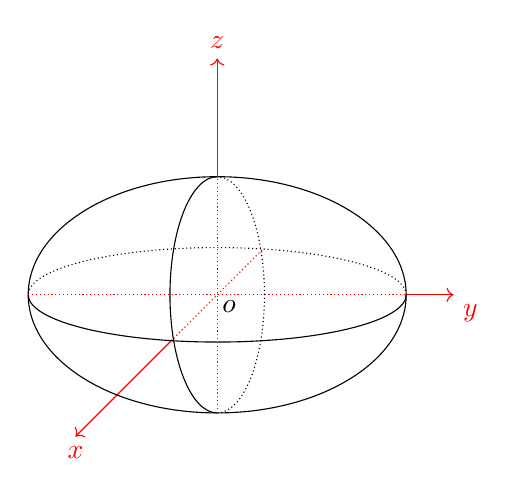
\begin{tikzpicture}[scale=3]
			\draw[red,->] (0.8,0) -- (1,0) node[anchor=north west]{$y$};
			\draw[red,->] (0,0.5) -- (0,1) node[anchor=south]{$z$};
			\draw[red,->] (-0.19,-0.19) -- (-0.6,-0.6) node[anchor=north]{$x$};
			\node at (0.05,-0.05) {$o$};
			\draw[densely dotted] (0.2,0) arc[start angle=0, end angle=90, x radius=0.2, y radius=0.5];
			\draw[densely dotted] (0,-0.5) arc[start angle=270, end angle=360, x radius=0.2, y radius=0.5];
			\draw (0,0.5) arc[start angle=90, end angle=270, x radius=0.2, y radius=0.5];
			\draw (0.8,0) arc[start angle=0, end angle=360, x radius=0.8, y radius=0.5];
			\draw[densely dotted] (0.8,0) arc[start angle=0, end angle=180, x radius=0.8, y radius=0.2];
			\draw (-0.8,0) arc[start angle=180, end angle=360, x radius=0.8, y radius=0.2];
			\draw[red,densely dotted] (-0.8,0) -- (0.8,0);
			\draw[red,densely dotted] (0,-0.5) -- (0,0.8);
			\draw[red,densely dotted] (0.19,0.19) -- (-0.19,-0.19);
		\end{tikzpicture}
		\caption{$\dfrac{x^{2}}{a^{2}} +\dfrac{y^{2}}{b^{2}}+\dfrac{z^{2}}{c^{2}}=1$}
	\end{figure}

	(b). 单叶双曲面 $\dfrac{x^{2}}{a^{2}} +\dfrac{y^{2}}{b^{2}} - \dfrac{z^{2}}{c^{2}}=1$

	\begin{figure}[H]
		\centering
		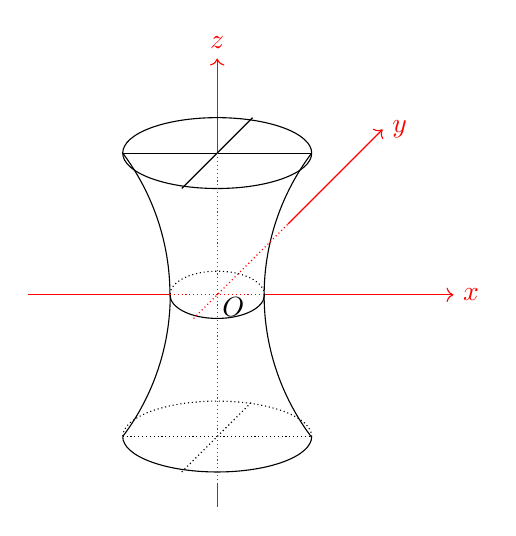
\begin{tikzpicture}[scale=3]
			\draw[red,->] (0.2,0) -- (1,0) node[right]{$x$};
			\draw[red,->] (0,0.6) -- (0,1) node[above]{$z$};
			\draw[red,->] (0.3,0.3) -- (0.7,0.7) node[right]{$y$};
			
			\draw (0.4,0.6) arc[start angle=0, end angle=360, x radius=0.4, y radius=0.15];
			\draw[densely dotted] (0.4,-0.6) arc[start angle=0, end angle=180, x radius=0.4, y radius=0.15];
			\draw (-0.4,-0.6) arc[start angle=180, end angle=360, x radius=0.4, y radius=0.15];
			
			\draw[densely dotted] (0.2,0) arc[start angle=0, end angle=180, x radius=0.2, y radius=0.1];
			\draw (-0.2,0) arc[start angle=180, end angle=360, x radius=0.2, y radius=0.1];
			
			\draw (0.4,0.6) arc[start angle=143, end angle=217, x radius=1, y radius=1];
			\draw (-0.4,-0.6) arc[start angle=323, end angle=360, x radius=1, y radius=1];
			\draw (-0.2,0) arc[start angle=0, end angle=37, x radius=1, y radius=1];
			
			\draw[red] (-0.8,0) -- (-0.2,0);
			\draw (-0.4,0.6) -- (0.4,0.6);
			\draw[red] (0,-0.8) -- (0,-0.9);
			\draw (-0.15,0.45) -- (0.15,0.75);
			\draw[densely dotted] (-0.4,-0.6) -- (0.4,-0.6);
			\draw[densely dotted] (-0.15,-0.75) -- (0.15,-0.45);
			\draw[red,densely dotted] (-0.2,0) -- (0.2,0);
			\draw[red,densely dotted] (0,-0.8) -- (0,0.6);
			\draw[red,densely dotted] (-0.1,-0.1) -- (0.3,0.3);
			\node at (-0.02,0.03) [below right] {$O$};
		\end{tikzpicture}
		\caption{$\dfrac{x^{2}}{a^{2}} +\dfrac{y^{2}}{b^{2}} - \dfrac{z^{2}}{c^{2}}=1$}
	\end{figure}

	(c). 双叶双曲面 $\dfrac{x^{2}}{a^{2}} - \dfrac{y^{2}}{b^{2}} - \dfrac{z^{2}}{c^{2}} = 1$

	\begin{figure}[H]
		\centering
		\begin{tikzpicture}[scale=3]
			\draw[red,->] (1.1,0) -- (1.4,0) node[right] {$x$};
			\draw[red,->] (0,-1.2) -- (0,1.2) node[above] {$z$}; 
			\draw[red,->] (-0.4,-0.5) -- (0.4,0.5) node[right] {$y$}; 
			
			\draw[densely dotted] (-0.9,0) arc[start angle=0, end angle=90, x radius=0.2, y radius=0.5];
			\draw[densely dotted] (-1.1,-0.5) arc[start angle=270, end angle=360, x radius=0.2, y radius=0.5];
			\draw (-1.1,0.5) arc[start angle=90, end angle=270, x radius=0.2, y radius=0.5];
			\draw (-0.4,0) arc[start angle=0, end angle=90, x radius=0.7, y radius=0.5];
			\draw (-1.1,-0.5) arc[start angle=270, end angle=360, x radius=0.7, y radius=0.5];
			\draw (-1.26,-0.25) arc[start angle=270, end angle=360, x radius=0.86, y radius=0.25];
			\draw[densely dotted] (-0.4,0) arc[start angle=0, end angle=90, x radius=0.54, y radius=0.25];
			\draw (1.3,0) arc[start angle=0, end angle=360, x radius=0.2, y radius=0.5];
			\draw (1.1,0.5) arc[start angle=90, end angle=270, x radius=0.7, y radius=0.5];
			\draw (0.4,0) arc[start angle=180, end angle=270, x radius=0.54, y radius=0.25];
			\draw[densely dotted] (1.26,0.25) arc[start angle=90, end angle=180, x radius=0.86, y radius=0.25];
			\draw[red] (-1.4,0) -- (-1.3,0);
			\draw[red] (-0.4,0) -- (0.4,0);
			\draw[densely dotted] (-1.1,0.5) -- (-1.1,-0.5);
			\draw[densely dotted] (-0.94,0.25) -- (-1.26,-0.25);
			\draw[red,densely dotted] (0.4,0) -- (1.1,0);
			\draw (0.94,-0.25) -- (1.26,0.25);
			\draw (1.1,0.5) -- (1.1,-0.5);
			\draw[red,densely dotted] (-1.3,0) -- (-0.4,0);
			\node at (0,0) [below right] {$O$};
		\end{tikzpicture}
		\caption{$\dfrac{x^{2}}{a^{2}} - \dfrac{y^{2}}{b^{2}} - \dfrac{z^{2}}{c^{2}} = 1$}
	\end{figure}

	(d). 椭圆抛物面 $\dfrac{x^{2}}{2p} + \dfrac{y^{2}}{2q} = z (p,q > 0)$

	\begin{figure}[H]
		\centering
		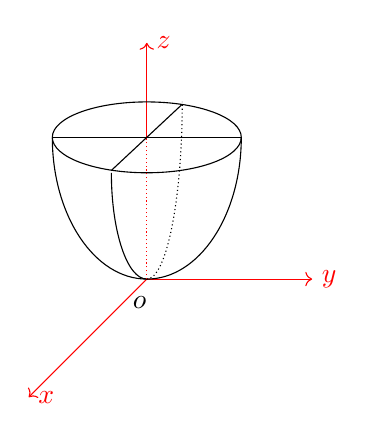
\begin{tikzpicture}[scale=3]
			\draw[red,->] (0,0) -- (-0.5,-0.5) node[right] {$x$};
			\draw[red,->] (0,0) -- (0.7,0) node[right] {$y$}; 
			\draw[red,->] (0,0.6) -- (0,1) node[right] {$z$}; 
			\draw (0.4,0.6) arc[start angle=0, end angle=360, x radius=0.4, y radius=0.15];
			\draw (-0.4,0.6) arc[start angle=180, end angle=360, x radius=0.4, y radius=0.6];
			\draw (-0.15,0.45) arc[start angle=180, end angle=270, x radius=0.15, y radius=0.45];
			\draw[densely dotted] (0,0) arc[start angle=270, end angle=360, x radius=0.15, y radius=0.75];
			\draw (-0.4,0.6) -- (0.4,0.6);
			\draw[red,densely dotted] (0,0) -- (0,0.6);
			\draw (-0.15,0.46) -- (0.15,0.74);
			\node at (-0.1,-0.1) [right] {$o$};
		\end{tikzpicture}
		\caption{$\dfrac{x^{2}}{2p} + \dfrac{y^{2}}{2q} = z (p,q > 0)$}
	\end{figure}
	
	(f). 椭圆锥面 $\dfrac{x^{2}}{a^{2}} + \dfrac{y^{2}}{b^{2}} = \dfrac{z^{2}}{c^{2}}$

	\begin{figure}[H]
		\centering
		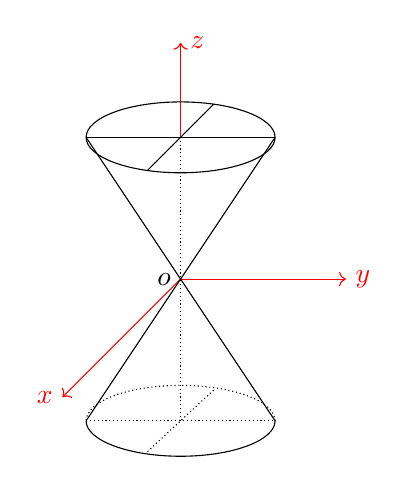
\begin{tikzpicture}[scale=3]
			\draw[red,->] (0,0) -- (-0.5,-0.5) node[left] {$x$};
			\draw[red,,->] (0,0) -- (0.7,0) node[right] {$y$}; 
			\draw[red,->] (0,0.6) -- (0,1) node[right] {$z$}; 
			\draw (0.4,0.6) arc[start angle=0, end angle=360, x radius=0.4, y radius=0.15];
			\draw[densely dotted] (0.4,-0.6) arc[start angle=0, end angle=180, x radius=0.4, y radius=0.15];
			\draw (-0.4,-0.6) arc[start angle=180, end angle=360, x radius=0.4, y radius=0.15];
			\draw (-0.4,0.6) -- (0.4,-0.6);
			\draw (0.4,0.6) -- (-0.4,-0.6);
			\draw (-0.4,0.6) -- (0.4,0.6);
			\draw[densely dotted] (-0.4,-0.6) -- (0.4,-0.6);
			\draw[densely dotted] (-0.14,-0.73) -- (0.14,-0.47);
			\draw[densely dotted] (0,-0.6) -- (0,0.6);
			\draw (-0.14,0.46) -- (0.14,0.74);
			\node at (0,0) [left] {$o$};
		\end{tikzpicture}
		\caption{$\dfrac{x^{2}}{a^{2}} + \dfrac{y^{2}}{b^{2}} = \dfrac{z^{2}}{c^{2}}$}
	\end{figure}

	(g). 双曲抛物面 $ - \dfrac{x^{2}}{2p} + \dfrac{y^{2}}{2q} = z (p,q > 0)$

	\begin{figure}[H]
		\centering
		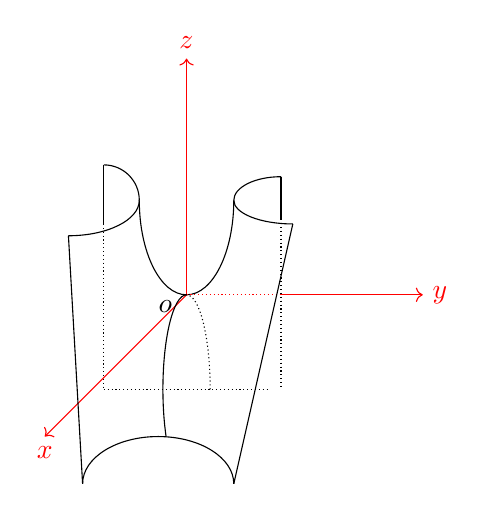
\begin{tikzpicture}[scale=3]
			\draw[red,->] (0.4,0) -- (1,0) node[right] {$y$};
			\draw[red,->] (0,0) -- (0,1) node[above] {$z$};
			\draw[red,->] (0,0) -- (-0.6,-0.6) node[below] {$x$};
			\draw (-0.2,0.4) arc[start angle=180, end angle=360, x radius=0.2, y radius=0.4];
			\draw (-0.2,0.4) arc[start angle=0, end angle=90, x radius=0.15, y radius=0.15];
			\draw (-0.5,0.25) arc[start angle=270, end angle=360, x radius=0.3, y radius=0.15];
			\draw (0.4,0.5) arc[start angle=90, end angle=180, x radius=0.2, y radius=0.1];
			\draw (0.2,0.4) arc[start angle=180, end angle=270, x radius=0.25, y radius=0.1];
			\draw (0.2,-0.8) arc[start angle=0, end angle=180, x radius=0.32, y radius=0.2];
			\draw[densely dotted] (0.1,-0.4) arc[start angle=0, end angle=90, x radius=0.1, y radius=0.4];
			\draw (0,0) arc[start angle=90, end angle=210, x radius=0.1, y radius=0.4];
			\draw[densely dotted] (-0.35,0.3) -- (-0.35,-0.4);
			\draw[densely dotted] (-0.35,-0.4) -- (0.35,-0.4);
			\draw[densely dotted] (0.4,0.5) -- (0.4,-0.4);
			\draw[red,densely dotted] (0,0) -- (0.4,0);
			\draw (0.4,0.5) -- (0.4,0.32);
			\draw (-0.35,0.55) -- (-0.35,0.3);
			\draw (-0.5,0.25) -- (-0.44,-0.8);
			\draw (0.45,0.3) -- (0.2,-0.8);
			\node at (-0.02, -0.05) [left]{$o$};
		\end{tikzpicture}
		\caption{$- \dfrac{x^{2}}{2p} + \dfrac{y^{2}}{2q} = z (p,q > 0)$}
	\end{figure}

	(h). 双曲抛物面 $z = xy$
	
	\begin{figure}[H]
		\centering
		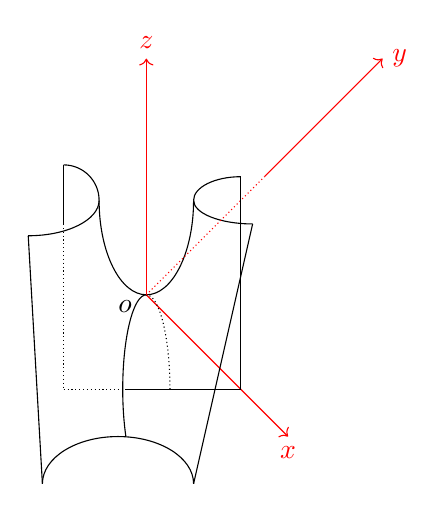
\begin{tikzpicture}[scale=3]
			\draw[red,->] (0.5,0.5) -- (1,1) node[right] {$y$};
			\draw[red,->] (0,0) -- (0,1) node[above] {$z$};
			\draw[red,->] (0,0) -- (0.6,-0.6) node[below] {$x$};
			\draw (-0.2,0.4) arc[start angle=180, end angle=360, x radius=0.2, y radius=0.4];
			\draw (-0.2,0.4) arc[start angle=0, end angle=90, x radius=0.15, y radius=0.15];
			\draw (-0.5,0.25) arc[start angle=270, end angle=360, x radius=0.3, y radius=0.15];
			\draw (0.4,0.5) arc[start angle=90, end angle=180, x radius=0.2, y radius=0.1];
			\draw (0.2,0.4) arc[start angle=180, end angle=270, x radius=0.25, y radius=0.1];
			\draw (0.2,-0.8) arc[start angle=0, end angle=180, x radius=0.32, y radius=0.2];
			\draw[densely dotted] (0.1,-0.4) arc[start angle=0, end angle=90, x radius=0.1, y radius=0.4];
			\draw (0,0) arc[start angle=90, end angle=210, x radius=0.1, y radius=0.4];
			\draw[densely dotted] (-0.35,0.3) -- (-0.35,-0.4);
			\draw[densely dotted] (-0.35,-0.4) -- (-0.09,-0.4);
			\draw (-0.09,-0.4) -- (0.4,-0.4);
			\draw (0.4,0.5) -- (0.4,-0.4);
			\draw[red,densely dotted] (0,0) -- (0.5,0.5);
			\draw (0.4,0.5) -- (0.4,0.32);
			\draw (-0.35,0.55) -- (-0.35,0.3);
			\draw (-0.5,0.25) -- (-0.44,-0.8);
			\draw (0.45,0.3) -- (0.2,-0.8);
			\node at (-0.02, -0.05) [left]{$o$};
		\end{tikzpicture}
		\caption{$z = xy$}
	\end{figure}

	(i). 椭圆柱面 $\dfrac{x^{2}}{a^{2}}+\dfrac{y^{2}}{b^{2}} = 1$
	
	\begin{figure}[H]
		\centering
		\begin{tikzpicture}[scale=3]
			\draw[red,->] (0,0.6) -- (0,1) node[right] {$z$};
			\draw[red,->] (0.3,0) -- (1,0) node[above] {$y$};
			\draw[red,->] (-0.1,-0.1) -- (-0.6,-0.6) node[below] {$x$};
			\draw (0.3,0.6) arc[start angle=0, end angle=360, x radius=0.3, y radius=0.1];
			\draw (-0.3,0) arc[start angle=180, end angle=360, x radius=0.3, y radius=0.1];
			\draw (-0.3,-0.4) arc[start angle=180, end angle=360, x radius=0.3, y radius=0.1];
			\draw[densely dotted] (0.3,0) arc[start angle=0, end angle=180, x radius=0.3, y radius=0.1];
			\draw[densely dotted] (0.3,-0.4) arc[start angle=0, end angle=180, x radius=0.3, y radius=0.1];
			\draw (-0.3,-0.4) -- (-0.3,0.6);
			\draw (0.3,-0.4) -- (0.3,0.6);
			\draw[red,densely dotted] (0,-0.5) -- (0,0.6);
			\draw[red,densely dotted] (-0.1,-0.1) -- (0.1,0.1);
			\draw[red,densely dotted] (-0.3,0) -- (0.3,0);
			\node at (0.1, -0.1) [below]{$o$};
		\end{tikzpicture}
		\caption{$\dfrac{x^{2}}{a^{2}}+\dfrac{y^{2}}{b^{2}} = 1$}
	\end{figure}
	

	(j). 双曲柱面 $\dfrac{x^{2}}{a^{2}} - \dfrac{y^{2}}{b^{2}} = 1$

	\begin{figure}[H]
		\centering
		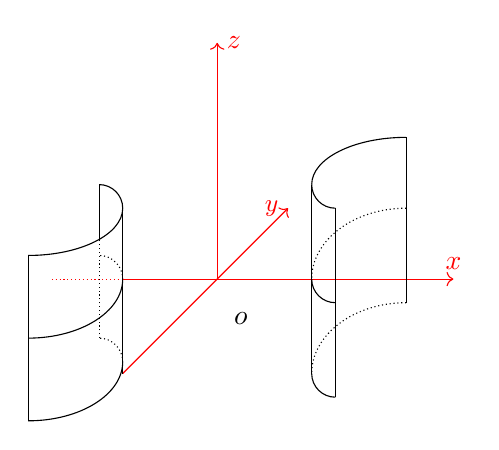
\begin{tikzpicture}[scale=3]
			\draw[red,->] (0,0) -- (0,1) node[right] {$z$};
			\draw[red,->] (0,0) -- (1,0) node[above] {$x$};
			\draw[red,->] (-0.4,-0.4) -- (0.3,0.3) node[left] {\small{$y$}};
			\draw (0.8,0.6) arc[start angle=90, end angle=180, x radius=0.4, y radius=0.2];
			\draw (0.4,0.4) arc[start angle=180, end angle=270, x radius=0.1, y radius=0.1];
			\draw (-0.4,0.3) arc[start angle=0, end angle=90, x radius=0.1, y radius=0.1];
			\draw (-0.8,0.1) arc[start angle=270, end angle=360, x radius=0.4, y radius=0.2];
			\draw (-0.8,-0.25) arc[start angle=270, end angle=360, x radius=0.4, y radius=0.25];
			\draw (-0.8,-0.6) arc[start angle=270, end angle=360, x radius=0.4, y radius=0.25];
			\draw[densely dotted] (-0.4,-0.35) arc[start angle=0, end angle=90, x radius=0.1, y radius=0.1];
			\draw[densely dotted] (-0.4,0) arc[start angle=0, end angle=90, x radius=0.1, y radius=0.1];
			\draw (0.4,0) arc[start angle=180, end angle=270, x radius=0.1, y radius=0.1];
			\draw (0.4,-0.4) arc[start angle=180, end angle=270, x radius=0.1, y radius=0.1];
			\draw[densely dotted] (0.8,0.3) arc[start angle=90, end angle=180, x radius=0.4, y radius=0.3];
			\draw[densely dotted] (0.8,-0.1) arc[start angle=90, end angle=180, x radius=0.4, y radius=0.3];
			\draw[densely dotted] (-0.5,-0.25) -- (-0.5,0.16);
			\draw[red,densely dotted] (-0.7,0) -- (-0.4,0);
			\draw[red] (-0.4,0) -- (0,0);
			\draw (-0.5,0.16) -- (-0.5,0.4);
			\draw (0.4,-0.4) -- (0.4,0.4);
			\draw (0.8,-0.1) -- (0.8,0.6);
			\draw (-0.4,0.3) -- (-0.4,-0.4);
			\draw (-0.8,0.1) -- (-0.8,-0.6);
			\draw (0.5,-0.5) -- (0.5,0.3);
			\node at (0.1, -0.1) [below]{$o$};
		\end{tikzpicture}
		\caption{$\dfrac{x^{2}}{a^{2}} - \dfrac{y^{2}}{b^{2}} = 1$}
	\end{figure}
	

	(k). 抛物柱面 $ y = ax^{2}$

	\begin{figure}[H]
		\centering
		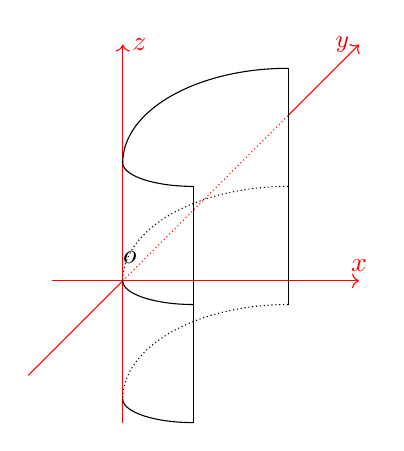
\begin{tikzpicture}[scale=3]
			\draw[red,->] (0,-0.6) -- (0,1) node[right] {$z$};
			\draw[red,->] (-0.3,0) -- (1,0) node[above] {$x$};
			\draw[red,->] (0.7,0.7) -- (1,1) node[left] {\small{$y$}};
			\draw[red,densely dotted] (0,0) -- (0.7,0.7);
			\draw[red] (-0.4,-0.4) -- (0,0);
			\draw (0.7,0.9) arc[start angle=90, end angle=180, x radius=0.7, y radius=0.4];
			\draw (0,0.5) arc[start angle=180, end angle=270, x radius=0.3, y radius=0.1];
			\draw (0,0) arc[start angle=180, end angle=270, x radius=0.3, y radius=0.1];
			\draw (0,-0.5) arc[start angle=180, end angle=270, x radius=0.3, y radius=0.1];
			\draw[densely dotted] (0.7,0.4) arc[start angle=90, end angle=180, x radius=0.7, y radius=0.4];
			\draw[densely dotted] (0.7,-0.1) arc[start angle=90, end angle=180, x radius=0.7, y radius=0.4];
			\draw (0.3,0.4) -- (0.3,-0.6);
			\draw (0.7,-0.1) -- (0.7,0.9);
			\node at (0.1, 0.1) [left]{$o$};
		\end{tikzpicture}
		\caption{$y = ax^{2}$}
	\end{figure}

	(3). 旋转曲面

	曲线 $\Gamma : \begin{cases}
	  F(x,y,z) = 0\\
	  G(x,y,z) = 0
	\end{cases}$ 绕直线 $L: \dfrac{x-x_{0}}{l} = \dfrac{y-y_{0}}{m} = \dfrac{z-z_{0}}{n}$ 旋转一周形成的旋转曲面, 直线 $L$ 的方向向量 
	$\boldsymbol{\tau} = (l,m,n)$

	设 $M_{1}(x_{1},y_{1},z_{1})$ 是曲线 $\Gamma$ 上任意一点, $P(x,y,z)$ 是 $M_{1}$ 绕直线 $L$ 旋转一周形成的纬圆上异于 $M_{1}$ 的一点:
	$$\begin{cases}
	  \boldsymbol{\tau} \perp \overrightarrow{M_{1}P} \\
	  |\overrightarrow{M_{1}M_{0}}| = |\overrightarrow{PM_{0}}|\\
	  F(x_{1},y_{1},z_{1}) = 0\\
	  G(x_{1},y_{1},z_{1}) = 0
	\end{cases}$$
\end{definition}
\subsection{空间曲线的切线和法平面}
\begin{definition}[曲线切线和法平面]
	
	(1).参数方程
	$$\begin{cases}
		x = f(t)\\
		y = g(t)\\
		z = h(t)
	\end{cases}, t \in [\alpha,\beta]$$
	
	在 $t=t_{0}$ 时,点 $P_{0}(x(t_{0}),y(t_{0}),z(t_{0}))$ 处切线的方向向量 $\boldsymbol{n}=(f'(t_{0}),g'(t_{0}),h'(t_{0}))$
	
	\textcolor{cyan}{切线方程}
	
	$$\dfrac{x-x_{0}}{f'(t_{0})}=\dfrac{y-y_{0}}{g'(t_{0})}=\dfrac{z-z_{0}}{h'(t_{0})}$$
	
	\textcolor{purplea}{法平面方程}
	
	$$f'(t_{0})(x-x_{0})+g'(t_{0})(y-y_{0})+h'(t_{0})(z-z_{0})=0$$
	
	(2). 一般式
	$$\begin{cases}
		F(x,y,z) = 0\\
		G(x,y,z) = 0
	\end{cases}$$
	
	点 $P_{0}(x_{0},y_{0},z_{0})$ 处切线的方向向量
	$$\boldsymbol{\tau} = 
	\begin{vmatrix}
	  \boldsymbol{i} & \boldsymbol{j} & \boldsymbol{k}\\
	  F_{x}' & F_{y}' & F_{z}'\\
	  G_{x}' & G_{y}' & G_{z}'
	\end{vmatrix} = (A,B,C)$$

	
	\textcolor{cyan}{切线方程}
	
	$$\dfrac{x-x_{0}}{A} = \dfrac{y-y_{0}}{B} = \dfrac{z-z_{0}}{C}$$
	
	\textcolor{purplea}{法平面方程}
	
	$$A(x-x_{0}) + B(y-y_{0}) + C(z-z_{0}) = 0$$
	
	
\end{definition}

\subsection{空间曲面的切平面和法线}
\begin{definition}
	
	(1). $F(x,y,z)=0$, 点 $P(x_{0},y_{0},z_{0})$ 处切平面法向量 $\boldsymbol{n} = \{F_{x}'(x_{0},y_{0},z_{0}),F_{y}'(x_{0},y_{0},z_{0}),F_{z}'(x_{0},y_{0},z_{0})\}$
	
	\textcolor{cyan}{切平面方程}
	
	$$F_{x}'(x_{0},y_{0},z_{0})(x-x_{0}) + F_{y}'(x_{0},y_{0},z_{0})(y-y_{0}) + F_{z}'(x_{0},y_{0},z_{0})(z-z_{0}) = 0$$

	\textcolor{purplea}{法线方程}
	
	$$\dfrac{x-x_{0}}{F_{x}'(x_{0},y_{0},z_{0})} = \dfrac{y-y_{0}}{F_{y}'(x_{0},y_{0},z_{0})}=\dfrac{z-z_{0}}{F_{z}'(x_{0},y_{0},z_{0})}$$
	
	(2). $z=f(x,y)$, 点 $P(x_{0},y_{0},z_{0})$ 处切平面法向量 $\boldsymbol{n} = \{f_{x}'(x_{0},y_{0}),f_{y}'(x_{0},y_{0}),-1\}$
	
	
	\textcolor{cyan}{切平面方程}

	$$f_{x}'(x_{0},y_{0})(x-x_{0}) + f_{y}'(x_{0},y_{0})(y-y_{0}) - (z-z_{0}) = 0$$
	
	\textcolor{purplea}{法线方程}
	
	$$\dfrac{x-x_{0}}{f_{x}'(x_{0},y_{0})} = \dfrac{y-y_{0}}{f_{y}'(x_{0},y_{0})} = \dfrac{z-z_{0}}{-1}$$
\end{definition}

\section{场论初步}

\subsection{方向导数}
\begin{definition}[方向导数]
	
	设三元函数 $u=u(x,y,z)$ 在点 $P(x_{0},y_{0},z_{0})$ 的某空间邻域内 $U\subset R^3$ 有定义,$l$ 是从 $P_{0}$ 出发的一条射线,$P(x,y,z)$ 为 $l$ 上且在 $U$ 中的任意一点: 
	$$\begin{cases}
		x-x_{0}=\Delta x=t\cos \alpha\\
		y-y_{0}=\Delta y=t\cos \beta\\
		z-z_{0}=\Delta z=t\cos \gamma
	\end{cases}$$ 
	
	$t=\sqrt{(\Delta x)^2+(\Delta y)^2+(\Delta z)^2}$ 表示 $|PP_{0}|$,如果下面极限存在: 

	$$\lim\lim\limits_{t\to 0}\frac{u(P)-u(P_{0})}{t}=\lim\lim\limits_{t\to 0}\frac{u(x_{0}+t\cos \alpha,y_{0}+t\cos \beta,z_{0}+t\cos \gamma)-u(x_{0},y_{0},z_{0})}{t}$$
	
	我们将此极限称为 $u=f(x,y,z)$ 在$P_{0}$ 处沿着 $l$ 的方向导数,记作 $\dfrac{\partial u}{\partial l}|_{P_{0}}$
\end{definition}

\begin{theorem}[方向导数计算公式]
	$$\dfrac{\partial u}{\partial \boldsymbol{l}}|_{P_{0}}=u_{x}'\cos \alpha+u_{y}'\cos \beta+u_{z}'\cos \gamma$$
	
	其中$\cos \alpha,\cos \beta,\cos \gamma$ 为方向 $\boldsymbol{l}$ 的方向余弦
\end{theorem}

\subsection{梯度}

\begin{definition}[梯度]
	
	设三元函数 $u=u(x,y,z)$ 在点 $P(x_{0},y_{0},z_{0})$ 处具有一阶偏导数,定义下面为 $u=u(x,y,z)$ 在 $ P_{0}(x_{0},y_{0},z_{0})$ 处的梯度: 
	
	$$\boldsymbol{guad}\ u|_{P_{0}}=(u_{x}'(P_{0}),u_{y}'(P_{0}),u_{z}'(P_{0}))$$
	
	
	梯度和方向导数之间的关系: 

	$$\dfrac{\partial u}{\partial l}|_{P_{0}}=\boldsymbol{guad}\ u|_{P_{0}}\cdot \boldsymbol{l}=\big|\boldsymbol{guad}\ u|_{P_{0}}\big| |l|\cos \theta$$
\end{definition}

\subsection{散度和旋度}

\begin{definition}[散度和旋度]
	设向量场 $\boldsymbol{A}(x,y,z)=P(x,y,z)\boldsymbol{i} + Q(x,y,z)\boldsymbol{j} + R(x,y,z)\boldsymbol{k}$
	
	\textcolor{cyan}{散度} 
	$$div\ \boldsymbol{A}=\dfrac{\partial P}{\partial x}+\dfrac{\partial Q}{\partial y}+\dfrac{\partial R}{\partial z}$$
	
	\textcolor{purplea}{旋度}
	$$rot \ \boldsymbol{A} = 
	\begin{vmatrix}
		\boldsymbol{i} & \boldsymbol{j} & \boldsymbol{k}\\
		\dfrac{\partial}{\partial x} & \dfrac{\partial}{\partial y} & \dfrac{\partial}{\partial z} \\
		P & Q & R
	\end{vmatrix}$$
\end{definition}



\chapterimage{chap12.jpg}
\chapter{三重积分(非数二)}

\section{三重积分定义和性质}

\begin{definition}[三重积分]
	设 $f(x, y, z)$ 是空间有界闭区域 $\Omega$ 上的有界函数, 将 $\Omega$ 任意分为 $n$ 个小闭区域
	$$\Delta v_{1}, \Delta v_{2}, \cdots, \Delta v_{n}$$
	其中 $\Delta v_{i}$ 表示第 $i$ 个小闭区域, 也表示第 $i$ 个小闭区域的体积, 在每一个 $\Delta v_{i}$ 中任意取一点 $(\xi_{i}, \eta_{i}, \zeta_{i})$, 作乘积 $f(\xi_{i},\eta_{i},\zeta_{i})\Delta v_{i}(i = 1,2,\cdots,n)$,
	并求和 $\sum_{i=1}^{n}f(\xi_{i},\eta_{i},\zeta_{i})\Delta v_{i}$, 如果当 $\lim\limits_{n \to +\infty}\{\lambda |\lambda = \max\{\Delta v_{i}\text{的直径}, i = 1,2,\cdots,n\}\} = 0$ 时, 求和的极限总是存在, 
	与 $\Delta v_{i}$ 的分法以及点 $(\xi_{i}, \eta_{i}, \zeta_{i})$ 的选取无关, 称此极限为函数 $f(x,y,z)$ 在闭区域 $\Omega$ 上的三重积分, 记作 $\iiint\limits_{\Omega}f(x,y,z)dv$

	$$\iiint\limits_{\Omega}f(x,y,z)dv = \lim\limits_{\lambda \to 0}\sum_{i=1}^{n}f(\xi_{i},\eta_{i},\zeta_{i})\Delta v_{i}$$
	
	其中 $f(x,y,z)$ 称为被积函数, $\Omega$ 称为积分区域, $f(x,y,z)dv$ 称为被积表达式, $dv$ 称为体积微元, $x,y,z$ 称为积分变量, $\sum\limits_{i=1}^{n} f(\xi_{i},\eta_{i},\zeta_{i})\Delta v_{i}$ 称为积分和

	\textcolor{cyan}{物理意义}

	设一物体占有 $Oxyz$ 上闭区域 $\Omega$, 在点 $(x,y,z)$ 处的密度为 $\rho(x,y,z)$, 假定 $\rho(x,y,z)$ 在 $\Omega$ 上连续, 物体质量 $M = \iiint\limits_{\Omega}\rho(x,y,z)dv$
\end{definition}

\begin{corollary}

	(1). 当 $f(x,y,z)$ 在闭区域 $\Omega$ 上连续时, 三重积分 $\iiint\limits_{\Omega}f(x,y,z)dv$ 一定存在; 当 $f(x,y,z)$ 在 $\Omega$ 上可积, $f(x,y,z)$ 在 $\Omega$ 上必有界

	(2). $\iint\limits_{\Omega}1dv = \iiint\limits_{\Omega}dv = V$, $V$ 是 $\Omega$ 的体积

	(3). 积分线性性质

	$$\iiint\limits_{\Omega}\left[k_{1}f(x,y,z)\pm k_{2}g(x,y,z)\right] dv=k_{1}\iiint\limits_{\Omega}f(x,y,z)dv \pm k_{2}\iiint\limits_{\Omega}g(x,y,z)dv$$
	
	(4). 积分的可加性

	设 $f(x,y,z)$ 在 $\Omega$ 上可积, 且 $\Omega_{1} \cap \Omega_{2} = \emptyset, \Omega_{1} \cup \Omega_{2} =\Omega$
	$$\iiint\limits_{\Omega}f(x,y,z)dv = \iiint\limits_{\Omega_{1}}f(x,y,z)dv + \iiint\limits_{\Omega_{2}}f(x,y,z)dv $$

	(5). 积分保号性

	设 $f(x,y,z)$ 和 $g(x,y,z)$ 在 $\Omega$ 上可积, 且在 $\Omega$ 上, $f(x,y,z)\leq g(x,y,z)$

	$$\iiint\limits_{\Omega}f(x,y,z)dv \leq \iiint\limits_{\Omega}g(x,y,z)dv \Rightarrow \big|\iiint\limits_{\Omega}f(x,y,z)dv\big| \leq \iiint\limits_{\Omega}\big|f(x,y,z)\big|dv$$

	(6). 估值定理

	设 $M,m$ 分别是 $f(x,y,z)$ 在 $\Omega$ 上的最大值和最小值, $V$ 是 $\Omega$ 的体积
	
	$$mV \leq \iiint\limits_{\Omega}f(x,y,z)dv \leq MV$$

	(7). 中值定理

	设 $f(x,y,z)$ 在 $\Omega$ 上连续, $V$ 是 $\Omega$ 的体积

	$$\exists (\xi,\eta,\zeta) \in \Omega,\ s.t.\ \iiint\limits_{\Omega}f(x,y,z)dv = f(\xi,\eta,\zeta)V $$

\end{corollary}

\section{三重积分对称性}

\begin{definition}[普通对称性]
	(1). $\Omega$ 关于平面 $xoz$ 对称

	$$\iiint\limits_{\Omega}f(x,y,z)dv = 
	\begin{cases}
		2\iiint\limits_{\Omega_{1}}f(x,y,z)dv & f(x,y,z) = f(x,-y,z)\\
		0                                     & f(x,y,z) = -f(x,-y,z)
	\end{cases}$$

	(2). $\Omega$ 关于平面 $yoz$ 对称

	$$\iiint\limits_{\Omega}f(x,y,z)dv =
	\begin{cases}
		2\iiint\limits_{\Omega_{1}}f(x,y,z)dv & f(x,y,z) = f(-x,y,z)\\
		0                                     & f(x,y,z) = -f(-x,y,z)
	\end{cases}$$

	(3). $\Omega$ 关于平面 $xoy$ 对称

	$$\iiint\limits_{\Omega}f(x,y,z)dv =
	\begin{cases}
		2\iiint\limits_{\Omega_{1}}f(x,y,z)dv & f(x,y,z) = f(x,y,-z)\\
		0                                     & f(x,y,z) = -f(x,y,-z)
	\end{cases}$$

\end{definition}

\begin{definition}[轮换对称性]
	若将 $x,y,z$ 任意两个交换位置后, 积分区域 $\Omega$ 保持不变

	$$\iiint\limits_{\Omega}f(x)dv=\iiint\limits_{\Omega}f(y)dv=\iiint\limits_{\Omega}f(z)dv$$
\end{definition}

\section{三重积分计算方法}


\begin{definition}[直角坐标系]
	(1). \textcolor{cyan}{先一后二}

	$$\iiint\limits_{\Omega}f(x,y,z)dv=\iint\limits_{D_{xy}}d\sigma \int_{z_{1}(x,y)}^{z_{2}(x,y)}f(x,y,z)dz$$
	
	一般用于空间区域 $\Omega$ 无侧面或者侧面为柱面, 转化为二重积分, 积分区域为空间区域 $\Omega$ 在 $xoy(yoz,xoz)$ 平面的投影
	
	(2). \textcolor{cyan}{先二后一}

	$$\iiint\limits_{\Omega}f(x,y,z)dv = \int_{a}^{b}dz\iint\limits_{D_{z}}f(x,y,z)d\sigma$$
	
	适用于旋转体, 旋转曲面方程 $z = z(x,y)$
\end{definition}

\begin{definition}[换元法]
	令 $\begin{cases}
	   x = x(u,v,w) \\
	   y = y(u,v,w) \\
	   z = z(u,v,w)
	\end{cases}$, 且 $(x,y,z)\to (u,v,w)$ 是一一映射, $x = x(u,v,w), y = y(u,v,w), z = z(u,v,w)$ 有一阶连续偏导数
	$$\begin{vmatrix}
		\dfrac{\partial (x,y,z)}{\partial (u,v,w)}
	  \end{vmatrix} = 
	\begin{Vmatrix}
	  \dfrac{\partial x}{\partial u} & \dfrac{\partial x}{\partial v} & \dfrac{\partial x}{\partial w} \\
	  \dfrac{\partial y}{\partial u} & \dfrac{\partial y}{\partial v} & \dfrac{\partial y}{\partial w} \\
	  \dfrac{\partial z}{\partial u} & \dfrac{\partial z}{\partial v} & \dfrac{\partial z}{\partial w}
	\end{Vmatrix}\neq 0$$

	$$\iiint\limits_{\Omega_{xyz}}f(x,y,z)dxdydz = \iiint\limits_{\Omega_{uvw}}f \left[x(u,v,w), y(u,v,w), z(u,v,w)\right] 
	\begin{vmatrix}
	  \dfrac{\partial (x,y,z)}{\partial (u,v,w)}
	\end{vmatrix}
	dudvdw$$
\end{definition}

\begin{definition}[柱面坐标系]
	令 $\begin{cases}
	  x = r\cos \theta, & \theta\in [0,2\pi] \\
	  y = r\sin \theta, & \theta\in [0,2\pi] \\
	  z = z
	\end{cases}$, 且 $(x,y,z)\to (r,\theta,z)$ 是一一映射, $x = r\cos \theta, y = r\sin \theta, z = z$ 有一阶连续偏导数
	
	$$\begin{vmatrix}
		\dfrac{\partial (x,y,z)}{\partial (r,\theta,z)}
	  \end{vmatrix} = 
	\begin{Vmatrix}
	  \dfrac{\partial x}{\partial r} & \dfrac{\partial x}{\partial \theta} & \dfrac{\partial x}{\partial z} \\
	  \dfrac{\partial y}{\partial r} & \dfrac{\partial y}{\partial \theta} & \dfrac{\partial y}{\partial z} \\
	  \dfrac{\partial z}{\partial r} & \dfrac{\partial z}{\partial \theta} & \dfrac{\partial z}{\partial z}
	\end{Vmatrix} = 
	\begin{Vmatrix}
	  \cos \theta & -r\sin \theta & 0 \\
	  \sin \theta & r\cos \theta & 0 \\
	  0 & 0 & 1
	\end{Vmatrix} = r$$
	
	$$\iiint\limits_{\Omega_{xyz}}f(x,y,z)dxdydz=\iint\limits_{\Omega_{r\theta z}}drd\theta \int_{z_{1}(r,\theta)}^{z_{2}(r,\theta)}rf(r\cos \theta,r\sin\theta,z)dz$$
\end{definition}

\begin{definition}[球面坐标系]
	令 $\begin{cases}
		x = r\sin\varphi\cos\theta, & \theta\in [0,2\pi]\\
		y = r\sin\varphi\sin\theta, & \theta\in [0,2\pi]\\\
		z = r\cos\varphi, & \varphi\in [0,\pi]
	\end{cases}$, 且 $(x,y,z) \to (r,\theta,\varphi)$ 是一一映射, $x = r\sin\varphi\cos\theta, y = r\sin\varphi\sin\theta, z = r\cos\varphi$ 有一阶连续偏导数

	$$\begin{vmatrix}
		\dfrac{\partial (x,y,z)}{\partial (r,\theta,\varphi)}
	\end{vmatrix} = 
	\begin{Vmatrix}
	  \dfrac{\partial x}{\partial r} & \dfrac{\partial x}{\partial \theta} & \dfrac{\partial x}{\partial \varphi} \\
	  \dfrac{\partial y}{\partial r} & \dfrac{\partial y}{\partial \theta} & \dfrac{\partial y}{\partial \varphi} \\
	  \dfrac{\partial z}{\partial r} & \dfrac{\partial z}{\partial \theta} & \dfrac{\partial z}{\partial \varphi}
	\end{Vmatrix} = 
	\begin{Vmatrix}
	  \sin\varphi\sin\theta & -r\sin\varphi\sin\theta & r\cos\varphi\cos\theta \\
	  \cos\varphi\cos\theta & r\sin\varphi\cos\theta & r\cos\varphi\sin\theta \\
	  \cos\varphi & 0 & -r\sin \varphi
	\end{Vmatrix} = r^{2}\sin\varphi$$

	$$\iiint\limits_{\Omega_{xyz}}f(x,y,z)dxdydz=\iiint\limits_{\Omega_{r\varphi\theta}}r^2\sin\varphi f(r\sin\varphi\cos\theta,r\sin\varphi\sin\theta,r\cos\varphi) drd\theta d\varphi$$
\end{definition}

\section{三重积分应用}
\begin{theorem}[重心公式]

	对于空间物体, 体密度 $\rho(x,y,z)$, $\Omega$ 是物体所占的空间区域, 重心 $O(\overline{x}, \overline{y}, \overline{z})$
	$$\begin{cases}
		\overline{x} = \dfrac{\iiint\limits_{\Omega}x\rho(x,y,z)dv}{\iiint\limits_{\Omega}\rho(x,y,z)dv} \\
		\overline{y} = \dfrac{\iiint\limits_{\Omega}y\rho(x,y,z)dv}{\iiint\limits_{\Omega}\rho(x,y,z)dv} \\
		\overline{z} = \dfrac{\iiint\limits_{\Omega}z\rho(x,y,z)dv}{\iiint\limits_{\Omega}\rho(x,y,z)dv}
	\end{cases}$$
	
	当密度函数为 $\rho(x,y,z)$ 为常数, 重心就是形心

	$$\begin{cases}
		\overline{x} = \dfrac{\iiint\limits_{\Omega}xdv}{\iiint\limits_{\Omega}dv} \\
		\overline{y} = \dfrac{\iiint\limits_{\Omega}ydv}{\iiint\limits_{\Omega}dv} \\
		\overline{z} = \dfrac{\iiint\limits_{\Omega}zdv}{\iiint\limits_{\Omega}dv}
	\end{cases}\Rightarrow 
	\begin{cases}
		\iiint\limits_{\Omega}xdv = \overline{x}\cdot V\\
		\iiint\limits_{\Omega}ydv = \overline{y}\cdot V\\
		\iiint\limits_{\Omega}zdv = \overline{z}\cdot V
	\end{cases}$$
\end{theorem}

\begin{theorem}[转动惯量 $I = \sum\limits_{i=1}^{n}m_{i}r_{i}^{2}$]

	对于空间物体, 体密度 $\rho(x,y,z)$, $\Omega$ 是物体所占的空间区域

	(1). $x$ 轴
	$$I_{x} = \iint\limits_{\Omega}(y^{2}+z^{2})\rho(x,y,z)dv$$

	(2). $y$ 轴

	$$I_{y} = \iint\limits_{\Omega}(x^{2}+z^{2})\rho(x,y,z)dv$$

	(3). $z$ 轴

	$$I_{z} = \iint\limits_{\Omega}(x^{2}+y^{2})\rho(x,y,z)dv$$

	(4). 原点 $O$

	$$I_{O} = \iint\limits_{\Omega}(x^{2}+y^{2}+z^{2})\rho(x,y,z)dv$$
\end{theorem}

\begin{theorem}[万有引力 $F = G\frac{m_{1}m_{2}}{r^{2}}$]

	对于空间物体, 体密度 $\rho(x,y,z)$, $\Omega$ 是物体所占的空间区域, 计算该物体对物体外一点 $M_{0}(x_{0},y_{0},z_{0})$ 处质量为 $m$ 的质点的引力 $\boldsymbol{F} = (F_{x},F_{y},F_{z})$
	
	\begin{eqnarray*}
		F_{x} & = & Gm \iiint\limits_{\Omega}\dfrac{\rho(x,y,z)}{(x-x_{0})^{2}+(y-y_{0})^{2}+(z-z_{0})^{2}}\cos\alpha dv \\
		      & = & Gm \iiint\limits_{\Omega}\dfrac{\rho(x,y,z)(x-x_{0})}{\left[(x-x_{0})^{2}+(y-y_{0})^{2}+(z-z_{0})^{2}\right]^{\frac{3}{2}}}
	\end{eqnarray*}

	\begin{eqnarray*}
		F_{y} & = & Gm \iiint\limits_{\Omega}\dfrac{\rho(x,y,z)}{(y-y_{0})^{2}+(y-y_{0})^{2}+(z-z_{0})^{2}}\cos\beta dv \\
		      & = & Gm \iiint\limits_{\Omega}\dfrac{\rho(x,y,z)(y-y_{0})}{\left[(x-x_{0})^{2}+(y-y_{0})^{2}+(z-z_{0})^{2}\right]^{\frac{3}{2}}}
	\end{eqnarray*}

	\begin{eqnarray*}
		F_{z} & = & Gm \iiint\limits_{\Omega}\dfrac{\rho(x,y,z)}{(z-z_{0})^{2}+(y-y_{0})^{2}+(z-z_{0})^{2}}\cos\gamma dv \\
		      & = & Gm \iiint\limits_{\Omega}\dfrac{\rho(x,y,z)(z-z_{0})}{\left[(x-x_{0})^{2}+(y-y_{0})^{2}+(z-z_{0})^{2}\right]^{\frac{3}{2}}}
	\end{eqnarray*}
\end{theorem}


\chapterimage{chap13.jpg}
\chapter{第一型曲线和曲面积分}

\section{第一型曲线积分}

\subsection{第一型曲线积分定义和性质}

\begin{definition}[第一型曲线积分]
	设 $L$ 是 $xoy$ 平面内一条光滑曲线弧, 函数 $f(x,y)$ 在 $L$ 上有界, 在 $L$ 上任意插入一系列的点 $M_{1}, M_{2}, \cdots, M_{n-1}$ 将 $L$ 分成 $n$ 小段, 设第 $i$ 段的弧长为 $\Delta s_{i}$, 
	在 第 $i$ 段上任意取一点 $(\zeta_{i},\eta_{i})$, 作乘积 $f(\zeta_{i},\eta_{i})\Delta s_{i}(i=1,2,\cdots,n)$, 并求和 $\sum\limits_{i=1}^{n}f(\zeta_{i},\eta_{i})\Delta s_{i}$, 当 
	$\lim\limits_{n \to +\infty}\{\lambda|\lambda = \max\{\Delta s_{i}\}, i =1,2,\cdots,n\} = 0$ 时, 求和极限存在, 
	且与 $\Delta s_{i}$ 的分法以及 $(\zeta_{i},\eta_{i})$ 的取法无关, 称此极限为函数 $f(x,y)$ 在曲线 $L$ 上对弧长的曲线积分
	或第一型曲线积分, 记作 $\int_{L}f(x,y)ds$
	$$\int_{L}f(x,y)ds = \lim\limits_{\lambda \to 0}\sum\limits_{i=1}^{n}f(\zeta_{i},\eta_{i})\Delta s_{i}$$ 

	其中 $f(x,y)$ 称为被积函数, $f(x,y)ds$ 称为被积表达式, $x,y$ 是积分变量, $L$ 是积分弧

	对于函数 $f(x,y,z)$ 在空间曲线 $\Gamma$ 上的第一型曲线积分
	$$\int_{\Gamma}f(x,y,z)ds = \lim\limits_{\lambda \to 0}\sum\limits_{i=1}^{n}f(\xi_{i},\eta_{i},\zeta_{i})\Delta s_{i}$$

	\textcolor{cyan}{物理意义}

	1. 设一物体在 $xoy$ 平面内一光滑曲线弧 $L$ 上, 物体在 $L$ 上的线密度为 $\rho(x,y)$, 则物体的质量 $m = \int_{L}\rho(x,y)ds$

	2. 设一物体在空间曲线 $\Gamma$ 上, 物体在 $\Gamma$ 上的线密度为 $\rho(x,y,z)$, 则物体的质量 $m = \int_{\Gamma}\rho(x,y,z)ds$
\end{definition}
\begin{corollary}

	(1). $\displaystyle{\int_{\Gamma} ds = l_{\Gamma}}$, 其中 $l_{\Gamma}$ 是 $\Gamma$ 的长度

	(2). 设 $f(x,y,z)$ 在 $\Gamma$ 上可积, 其在 $\Gamma$ 上必有界

	(3). 积分线性性质
	$$\int_{\Gamma}\left[k_{1}f(x,y,z) + k_{2} g(x,y,z)\right]ds = k_{1}\int_{\Gamma}f(x,y,z)ds+k_{2}\int_{\Gamma}g(x,y,z)ds$$

	(4). 积分可加性

	设 $f(x,y,z)$ 在 $\Gamma$ 上可积, 且 $\Gamma_{1}\cap \Gamma_{2}=\emptyset, \Gamma_{1}\cup \Gamma_{2}=\Gamma$

	$$\int_{\Gamma}f(x,y,z)ds = \int_{\Gamma_{1}}f(x,y,z)ds + \int_{\Gamma_{2}}f(x,y,z)ds$$

	(5). 积分保号性

	设 $f(x,y,z), g(x,y,z)$ 在 $\Gamma$ 上可积, 且在 $\Gamma$ 上 $f(x,y,z) \leq g(x,y,z)$
	$$\int_{\Gamma}f(x,y,z)ds \leq \int_{\Gamma}g(x,y,z)ds\Rightarrow \big|\int_{\Gamma}f(x,y,z)ds\big| \leq \int_{\Gamma}\big|f(x,y,z)\big|ds$$

	(6). 估值定理
	设 $M,m$ 分别是 $f(x,y,z)$ 在 $\Gamma$ 上的最大值和最小值, $l_{\Gamma}$ 的长度
	$$ml_{\Gamma} \leq \int_{\Gamma}f(x,y,z)ds \leq Ml_{\Gamma}$$

	(7). 中值定理

	设 $f(x,y,z)$ 在 $\Gamma$ 上连续, $l_{\Gamma}$ 是 $\Gamma$ 的长度

	$$\exists (\xi,\eta,\zeta)\in \Gamma,\ s.t.\ \int_{\Gamma}f(x,y,z) ds = f(\xi,\eta,\zeta)l_{\Gamma}$$
\end{corollary}

\subsection{第一型曲线积分的对称性}

\begin{definition}[普通对称性]
	(1). $\Gamma$ 关于平面 $xoz$ 对称

	$$\int_{\Gamma}f(x,y,z)ds = 
	\begin{cases}
		2\int_{\Gamma_{1}}f(x,y,z)ds & f(x,y,z) = f(x,-y,z)\\
		0                                     & f(x,y,z) = -f(x,-y,z)
	\end{cases}$$

	(2). $\Gamma$ 关于平面 $yoz$ 对称

	$$\int_{\Gamma}f(x,y,z)ds =
	\begin{cases}
		2\int_{\Gamma_{1}}f(x,y,z)ds & f(x,y,z) = f(-x,y,z)\\
		0                                     & f(x,y,z) = -f(-x,y,z)
	\end{cases}$$

	(3). $\Gamma$ 关于平面 $xoy$ 对称

	$$\int_{\Gamma}f(x,y,z)ds =
	\begin{cases}
		2\int_{\Gamma_{1}}f(x,y,z)ds & f(x,y,z) = f(x,y,-z)\\
		0                                     & f(x,y,z) = -f(x,y,-z)
	\end{cases}$$
\end{definition}

\begin{definition}[轮换对称性]
	若将 $x,y,z$ 任意两个交换位置后, 积分区域 $\Gamma$ 保持不变

	$$\int_{\Gamma}f(x)ds=\int_{\Gamma}f(y)ds=\int_{\Gamma}f(z)ds$$
\end{definition}

\subsection{第一型曲线积分计算}

\begin{theorem}[平面曲线]
	
	(1). $L: y=f(x), x\in[a,b]$
	
	$$\int_{L}f(x,y)ds=\int_{a}^{b}f(x,y)\sqrt{1+[f'(x)]^2}dx$$
	
	(2). $L: \begin{cases}
		x = x(t)\\
		y = y(t)
	\end{cases} t\in[\alpha,\beta]$
	
	$$\int_{L}f(x,y)ds=\int_{\alpha}^{\beta}f\left[x(t),y(t)\right]\sqrt{[x'(t)]^2+[y'(t)]^2}dt$$
	
	(3). $L: r=r(\theta), \theta\in[\theta_{1},\theta_{2}]$
	
	$$\int_{L}f(x,y)ds=\int_{\theta_{1}}^{\theta_{2}}f(r\cos \theta,r\sin\theta)\sqrt{[r(\theta)]^2+[r'(\theta)]^2}d\theta$$
\end{theorem}
\begin{theorem}[空间曲线]
	
	$$\begin{cases}
		x = x(t)\\
		y = y(t)\\
		z = z(t)
	\end{cases} t\in[\alpha,\beta]\Rightarrow 
	ds=\sqrt{[x'(t)]^{2}+[y'(t)]^{2}+[z'(t)]^{2}}dt$$
	
	$$\int_{\Gamma}f(x,y,z)ds=\int_{\alpha}^{\beta}f \left[ x(t),y(t),z(t)\right]\sqrt{[x'(t)]^{2}+[y'(t)]^{2}+[z'(t)]^{2}}dt$$
\end{theorem}

\section{第一型曲面积分}
\subsection{第一型曲面积分定义和性质}
\begin{definition}[第一型曲面积分]
	设曲面 $\Sigma$ 是光滑的, 函数 $f(x,y,z)$ 在 $\Sigma$ 上有界, 将 $\Sigma$ 任意分为 $n$ 个小块 $\Delta \Sigma_{i}$, $\Delta S_{i}$ 表示曲面 $\Delta\Sigma_{i}$ 的面积, 
	在 $\Delta\Sigma_{i}$ 上任意取一点 $(\xi_{i},\eta_{i},\zeta_{i})$, 作乘积 $f(\xi_{i},\eta_{i},\zeta_{i})\Delta S_{i}(i=1,2,\cdots,n)$, 并求和 
	$\sum\limits_{i=1}^{n}f(\xi_{i},\eta_{i},\zeta_{i})S_{i}$, 当 $\lim\limits_{n \to +\infty}\{\lambda|\lambda = \max\{S_{i}\}, i =1,2,\cdots,n\} = 0$ 
	时, 极限 $\lim\limits_{\lambda \to 0}\sum\limits_{i=1}^{n}f(\xi_{i},\eta_{i},\zeta_{i})\Delta S_{i}$ 存在, 且与 $\Delta\Sigma_{i}$ 的分法和 $(\xi_{i},\eta_{i},\zeta_{i})$ 
	的取法无关, 称此极限为函数 $f(x,y,z)$ 在曲面 $\Sigma$ 上对面积的曲面积分或第一型曲面积分, 记作 $\iint\limits_{\Sigma}f(x,y,z)dS$

	$$\iint\limits_{\Sigma}f(x,y,z)dS = \lim\limits_{\lambda \to 0}\sum\limits_{i=1}^{n}f(\xi_{i},\eta_{i},\zeta_{i})\Delta S_{i}$$

	其中 $f(x,y,z)$ 称为被积函数, $f(x,y,z)dS$ 称为被积表达式, $x,y,z$ 是积分变量, $\Sigma$ 是积分曲面

	\textcolor{cyan}{物理意义}

	设一曲面物体 $\Sigma$, 曲面密度为 $\rho(x,y,z)$, 则物体的质量 $m = \iint\limits_{\Sigma}\rho(x,y,z)dS$
\end{definition}

\begin{corollary}

	(1). $\displaystyle{\int_{\Sigma} dS = S}$, 其中 $S$ 是 $\Sigma$ 的面积

	(2). 设 $f(x,y,z)$ 在 $\Sigma$ 上可积, 其在 $\Sigma$ 上必有界

	(3). 积分线性性质
	$$\iint\limits_{\Sigma}\left[k_{1}f(x,y,z) + k_{2} g(x,y,z)\right]dS = k_{1}\iint\limits_{\Sigma}f(x,y,z)dS+k_{2}\iint\limits_{\Sigma}g(x,y,z)dS$$

	(4). 积分可加性

	设 $f(x,y,z)$ 在 $\Sigma$ 上可积, 且 $\Sigma_{1}\cap \Sigma_{2}=\emptyset, \Sigma_{1}\cup \Sigma_{2}=\Sigma$

	$$\iint\limits_{\Sigma}f(x,y,z)dS = \iint\limits_{\Sigma_{1}}f(x,y,z)dS + \iint\limits_{\Sigma_{2}}f(x,y,z)dS$$

	(5). 积分保号性

	设 $f(x,y,z), g(x,y,z)$ 在 $\Sigma$ 上可积, 且在 $\Sigma$ 上 $f(x,y,z) \leq g(x,y,z)$

	$$\iint\limits_{\Sigma}f(x,y,z)dS \leq \iint\limits_{\Sigma}g(x,y,z)dS\Rightarrow 
	\big|\iint\limits_{\Sigma}f(x,y,z)dS\big| \leq \iint\limits_{\Sigma}\big|f(x,y,z)\big|dS$$

	(6). 估值定理
	
	设 $M,m$ 分别是 $f(x,y,z)$ 在 $\Sigma$ 上的最大值和最小值, $S_{\Sigma}$ 表示 $\Sigma$ 的面积 
	
	$$mS_{\Sigma} \leq \iint\limits_{\Sigma}f(x,y,z)dS \leq MS_{\Sigma}$$

	(7). 中值定理

	设 $f(x,y,z)$ 在 $\Sigma$ 上连续, $S_{\Sigma}$ 是 $\Sigma$ 的面积

	$$\exists (\xi,\eta,\zeta)\in \Sigma,\ s.t.\ \iint\limits_{\Sigma}f(x,y,z) dS = f(\xi,\eta,\zeta)S_{\Sigma}$$
\end{corollary}

\subsection{第一型曲面积分的对称性}

\begin{definition}[普通对称性]
	(1). $\Sigma$ 关于平面 $xoz$ 对称

	$$\iint\limits_{\Sigma}f(x,y,z)dS = 
	\begin{cases}
		2\iint\limits_{\Sigma_{1}}f(x,y,z)dS & f(x,y,z) = f(x,-y,z)\\
		0                                    & f(x,y,z) = -f(x,-y,z)
	\end{cases}$$

	(2). $\Sigma$ 关于平面 $yoz$ 对称

	$$\iint\limits_{\Sigma}f(x,y,z)dS =
	\begin{cases}
		2\iint\limits_{\Sigma_{1}}f(x,y,z)dS & f(x,y,z) = f(-x,y,z)\\
		0                                    & f(x,y,z) = -f(-x,y,z)
	\end{cases}$$

	(3). $\Sigma$ 关于平面 $xoy$ 对称

	$$\iint\limits_{\Sigma}f(x,y,z)dS =
	\begin{cases}
		2\iint\limits_{\Sigma_{1}}f(x,y,z)dS & f(x,y,z) = f(x,y,-z)\\
		0                             & f(x,y,z) = -f(x,y,-z)
	\end{cases}$$
\end{definition}

\begin{definition}[轮换对称性]
	若将 $x,y,z$ 任意两个交换位置后, 积分区域 $\Sigma$ 保持不变

	$$\iint\limits_{\Sigma}f(x)dS=\iint\limits_{\Sigma}f(y)dS=\iint\limits_{\Sigma}f(z)dS$$
\end{definition}

\subsection{第一型曲面积分计算}
\begin{theorem}[投影法]
	1. 曲面投影 $xoy$ 平面

	设曲面 $\Sigma$ 的方程为 $z=z(x,y)$, 则 $\Sigma$ 的面积元素 $dS = \sqrt{1+\left(\dfrac{\partial z}{\partial x}\right)^{2}+\left(\dfrac{\partial z}{\partial y}\right)^{2}}dxdy$

	$$\iint\limits_{\Sigma}f(x,y,z)dS = \iint\limits_{D}f(x,y,z(x,y))\sqrt{1+\left(\dfrac{\partial z}{\partial x}\right)^{2}+\left(\dfrac{\partial z}{\partial y}\right)^{2}}dxdy$$

	2. 曲面投影 $yoz$ 平面

	设曲面 $\Sigma$ 的方程为 $x=x(y,z)$, 则 $\Sigma$ 的面积元素 $dS = \sqrt{1+\left(\dfrac{\partial x}{\partial y}\right)^{2}+\left(\dfrac{\partial x}{\partial z}\right)^{2}}dydz$

	$$\iint\limits_{\Sigma}f(x,y,z)dS = \iint\limits_{D}f(x(y,z),y,z)\sqrt{1+\left(\dfrac{\partial x}{\partial y}\right)^{2}+\left(\dfrac{\partial x}{\partial z}\right)^{2}}dydz$$

	3. 曲面投影 $xoz$ 平面

	设曲面 $\Sigma$ 的方程为 $y=y(x,z)$, 则 $\Sigma$ 的面积元素 $dS = \sqrt{1+\left(\dfrac{\partial y}{\partial x}\right)^{2}+\left(\dfrac{\partial y}{\partial z}\right)^{2}}dxdz$

	$$\iint\limits_{\Sigma}f(x,y,z)dS = \iint\limits_{D}f(x,y(x,z),z)\sqrt{1+\left(\dfrac{\partial y}{\partial x}\right)^{2}+\left(\dfrac{\partial y}{\partial z}\right)^{2}}dxdz$$

\end{theorem}
\section{第一型曲线积分和曲面积分应用}

1. \textcolor{purplec}{曲线长度和曲面面积}

\begin{theorem}[曲线弧长和曲面面积]

	$$L_{\Gamma} = \int_{\Gamma} ds$$

	$$S_{\Sigma} = \iint\limits_{\Sigma}dS$$
\end{theorem}

2. \textcolor{cyan}{重心}

\begin{theorem}[重心公式]

	(1). 光滑曲线, 对于光滑曲线 $\Gamma$, 线密度 $\rho(x,y,z)$, 重心 $O(\overline{x}, \overline{y}, \overline{z})$
	$$\begin{cases}
		\overline{x} = \dfrac{\int_{\Gamma}x\rho(x,y,z)ds}{\int_{\Gamma}\rho(x,y,z)ds} \\
		\overline{y} = \dfrac{\int_{\Gamma}y\rho(x,y,z)ds}{\int_{\Gamma}\rho(x,y,z)ds} \\
		\overline{z} = \dfrac{\int_{\Gamma}z\rho(x,y,z)ds}{\int_{\Gamma}\rho(x,y,z)ds}
	\end{cases}$$
	
	当密度函数为 $\rho(x,y,z)$ 为常数, 重心就是形心

	$$\begin{cases}
		\overline{x} = \dfrac{\int_{\Gamma}xds}{\int_{\Gamma}ds} \\
		\overline{y} = \dfrac{\int_{\Gamma}yds}{\int_{\Gamma}ds} \\
		\overline{z} = \dfrac{\int_{\Gamma}zds}{\int_{\Gamma}ds}
	\end{cases}\Rightarrow 
	\begin{cases}
		\int_{\Gamma}xds = \overline{x}\cdot l_{\Gamma}\\
		\int_{\Gamma}yds = \overline{y}\cdot l_{\Gamma}\\
		\int_{\Gamma}zds = \overline{z}\cdot l_{\Gamma}
	\end{cases}$$

	(2). 光滑曲面, 对于光滑曲面 $\Sigma$, 曲面密度 $\rho(x,y,z)$, 重心 $O(\overline{x}, \overline{y}, \overline{z})$

	$$\begin{cases}
		\overline{x} = \dfrac{\int_{\Sigma}x\rho(x,y,z)dS}{\int_{\Sigma}\rho(x,y,z)dS} \\
		\overline{y} = \dfrac{\int_{\Sigma}y\rho(x,y,z)dS}{\int_{\Sigma}\rho(x,y,z)dS} \\
		\overline{z} = \dfrac{\int_{\Sigma}z\rho(x,y,z)dS}{\int_{\Sigma}\rho(x,y,z)dS}
	\end{cases}$$
	
	当密度函数为 $\rho(x,y,z)$ 为常数, 重心就是形心

	$$\begin{cases}
		\overline{x} = \dfrac{\int_{\Sigma}xdS}{\int_{\Sigma}dS} \\
		\overline{y} = \dfrac{\int_{\Sigma}ydS}{\int_{\Sigma}dS} \\
		\overline{z} = \dfrac{\int_{\Sigma}zdS}{\int_{\Sigma}dS}
	\end{cases}\Rightarrow 
	\begin{cases}
		\int_{\Sigma}xdS = \overline{x}\cdot S_{\Sigma}\\
		\int_{\Sigma}ydS = \overline{y}\cdot S_{\Sigma}\\
		\int_{\Sigma}zdS = \overline{z}\cdot S_{\Sigma}
	\end{cases}$$
\end{theorem}

3. \textcolor{purplea}{转动惯量}
\begin{definition}[转动惯量: $I=mr^2$]
	
	(1). 光滑曲线, 对于光滑曲线 $\Gamma$, 线密度 $\rho(x,y,z)$
	
	对 $x$ 轴: $I_{x}=\int\limits_{L}(y^2+z^2)\rho(x,y,z)ds$
	
	对 $y$ 轴: $I_{y}=\int\limits_{L}(x^2+z^2)\rho(x,y,z)ds$
	
	对 $z$ 轴: $I_{z}=\int\limits_{L}(x^2+y^2)\rho(x,y,z)ds$
	
	对坐标原点 $O$: $I_{O}=\int\limits_{L}(x^2+y^2+z^2)\rho(x,y,z)ds$
	
	(2). 光滑曲面, 对于光滑曲线 $\Sigma$, 面密度 $\rho(x,y,z)$
	
	对 $x$ 轴: $I_{x}=\iint\limits_{\Sigma}(y^2+z^2)\rho(x,y,z)dS$
	
	对 $y$ 轴: $I_{y}=\iint\limits_{\Sigma}(x^2+z^2)\rho(x,y,z)dS$
	
	对 $z$ 轴: $I_{z}=\iint\limits_{\Sigma}(x^2+y^2)\rho(x,y,z)dS$
	
	对坐标原点 $O$: $I_{O}=\iint\limits_{\Sigma}(x^2+y^2+z^2)\rho(x,y,z)dS$
	
\end{definition}

4. \textcolor{purpleb}{万有引力}
\begin{definition}[引力公式: $F=\dfrac{GMm}{r^2}$]	

	(1). 光滑曲线, 对于光滑曲线 $\Gamma$, 线密度 $\rho(x,y,z)$

	$$F_{x}=Gm\int\limits_{\Gamma}\dfrac{\rho(x,y,z)(x-x_{0})}{[(x-x_{0})^2+(y-y_{0})^2+(z-z_{0})^2]^{\frac{3}{2}}}ds$$
	$$F_{y}=Gm\int\limits_{\Gamma}\dfrac{\rho(x,y,z)(y-y_{0})}{[(x-x_{0})^2+(y-y_{0})^2+(z-z_{0})^2]^{\frac{3}{2}}}ds$$
	$$F_{z}=Gm\int\limits_{\Gamma}\dfrac{\rho(x,y,z)(z-z_{0})}{[(x-x_{0})^2+(y-y_{0})^2+(z-z_{0})^2]^{\frac{3}{2}}}ds$$
	
	(2). 光滑曲面, 对于光滑曲面 $\Sigma$, 面密度 $\rho(x,y,z)$
	$$F_{x}=Gm\iint\limits_{\Sigma}\dfrac{\rho(x,y,z)(x-x_{0})}{[(x-x_{0})^2+(y-y_{0})^2+(z-z_{0})^2]^{\frac{3}{2}}}dS$$
	$$F_{y}=Gm\iint\limits_{\Sigma}\dfrac{\rho(x,y,z)(y-y_{0})}{[(x-x_{0})^2+(y-y_{0})^2+(z-z_{0})^2]^{\frac{3}{2}}}dS$$
	$$F_{z}=Gm\iint\limits_{\Sigma}\dfrac{\rho(x,y,z)(z-z_{0})}{[(x-x_{0})^2+(y-y_{0})^2+(z-z_{0})^2]^{\frac{3}{2}}}dS$$
\end{definition}


\chapterimage{chap14.jpg}
\chapter{第二型曲线和曲面积分}

\section{第二型曲线积分}
\subsection{第二型曲线积分定义和性质}
\begin{definition}[第二型曲线积分]
	在变力场中, $\boldsymbol{F} = P(x,y)\boldsymbol{i} + Q(x,y)\boldsymbol{j}$ 沿着曲线 $L$ 从 $A$ 点到 $B$ 点的做功

	二维平面
	$$W = \int_{L}\boldsymbol{F}\cdot d\boldsymbol{s} = \int_{L}P(x,y)dx+Q(x,y)dy$$

	三维空间
	$$W = \int_{\Gamma}\boldsymbol{F}\cdot d\boldsymbol{s} = \int_{\Gamma}P(x,y,z)dx+Q(x,y,z)dy+R(x,y,z)dz$$
\end{definition}
\begin{corollary}
	(1). 线性性质

	$$\int_{\Gamma}(k_{1}\boldsymbol{F_{1}}\pm \boldsymbol{F_{2}})d\boldsymbol{s} = k_{1}\int_{\Gamma}\boldsymbol{F_{1}}d\boldsymbol{s} + k_{2}\int_{\Gamma}\boldsymbol{F_{2}}d\boldsymbol{s}$$
	(2). 积分有向性
	
	$$\int_{\mathop{AB}\limits^{\frown}}\boldsymbol{F}d\boldsymbol{s} = - \int_{\mathop{BA}\limits^{\frown}}\boldsymbol{F}d\boldsymbol{s}$$
	
	(3). 积分可加性
	
	$$\int_{\mathop{AB}\limits^{\frown}}\boldsymbol{F}d\boldsymbol{s} = \int_{\mathop{AC}\limits^{\frown}}\boldsymbol{F}d\boldsymbol{s} + \int_{\mathop{CB}\limits^{\frown}}\boldsymbol{F}d\boldsymbol{s}$$
\end{corollary}
\subsection{第二型曲线积分计算}
\subsubsection{参数方程转定积分}
\begin{theorem}
	1. 二维平面
	$$ L = \begin{cases}
		x = x(t)\\
		y = y(t)
	\end{cases}, t\in[\alpha,\beta]$$
	$$\int_{L}P(x,y)dx+Q(x,y)dy = \int_{\alpha}^{\beta}[P(x(t),y(t))x'(t)+Q(x(t),y(t))y'(t)]dt$$

	2. 三维空间
	$$\Gamma = \begin{cases}
		x = x(t)\\
		y = y(t)\\
		z = z(t)
	\end{cases}, t\in[\alpha,\beta]$$
	\begin{eqnarray*}
		\int_{\Gamma}P(x,y,z)dx+Q(x,y,z)dy+R(x,y,z)dz & = & \int_{\alpha}^{\beta}P(x(t),y(t),z(t))x'(t)dt \\
		& + & Q(x(t),y(t),z(t))y'(t)dt \\
		& + & R(x(t),y(t),z(t))z'(t)dt
	\end{eqnarray*}
\end{theorem}
\subsubsection{格林公式}
\begin{theorem}[格林公式]
	设平面有界区域 $D$ 由光滑曲线 $L$ 围成, $L$ 取正向(左手在内侧), $P(x,y),Q(x,y)$ 在 $D$ 上有一阶连续偏导数

	$$\oint_{L}P(x,y)dx+Q(x,y)dy=\iint\limits_{D}\left(\frac{\partial Q}{\partial x}-\frac{\partial P}{\partial y}\right)dxdy$$
\end{theorem}
\begin{itemize}
	\item $L$ 是非封闭区域, 且在区域 $D$ 内满足 $\dfrac{\partial P}{\partial y} \neq \dfrac{\partial Q}{\partial x}$, 补线使其成为封闭区域
	\item $L$ 是封闭区域, 且在区域 $D$ 内有奇点, 且除奇点之外满足 $\dfrac{\partial P}{\partial y} = \dfrac{\partial Q}{\partial x}$
	$$\oint_{L}Pdx+Qdy = \oint_{L_{1}}Pdx+Qdy$$
	\item 平面曲线积分与路径无关 $\Leftrightarrow \dfrac{\partial P}{\partial y} = \dfrac{\partial Q}{\partial x} \Leftrightarrow u = Pdx+ Qdy$ 
\end{itemize}
\subsubsection{斯托克斯公式}
\begin{theorem}[斯托克斯公式]
	设 $\Omega$ 是某空间区域, $\Sigma$ 是 $\Omega$ 内分片光滑有向曲面, $\Gamma$ 是 $\Sigma$ 的边界, 方向和 $\Sigma$ 法向量成右手系, 函数 $P(x,y,z),Q(x,y,z),R(x,y,z)$ 在 $\Omega$ 内有连续的一阶偏导数

	$$\oint_{\Gamma}Pdx+Qdy+Rdz=\iint\limits_{\Sigma}
	\begin{vmatrix}
		\cos\alpha&\cos\beta&\cos\gamma\\
		\dfrac{\partial}{\partial x}&\dfrac{\partial }{\partial y}&\dfrac{\partial}{\partial z}\\
		P&Q&R
	\end{vmatrix}dS $$
	$$\oint_{\Gamma}Pdx+Qdy+Rdz=\iint\limits_{\Sigma}
	\begin{vmatrix}
		dydz&dxdz&dxdy\\
		\dfrac{\partial}{\partial x}&\dfrac{\partial }{\partial y}&\dfrac{\partial}{\partial z}\\
		P&Q&R
	\end{vmatrix}$$
\end{theorem}

\section{第二型曲面积分}
\subsection{第二型曲面积分定义和性质}
\begin{definition}[第二型曲线积分]
	在向量场场中, 存在向量函数 $\boldsymbol{F}(x,y,z) = P(x,y,z)\boldsymbol{i} + Q(x,y,z)\boldsymbol{j} + R(x,y,z)\boldsymbol{k}$, $\boldsymbol{\Sigma}$ 是
	向量场中某一有向光滑曲面, $\boldsymbol{n}$ 是 $\boldsymbol{\Sigma}$ 的单位法向量, $\boldsymbol{F}$ 在 $\boldsymbol{\Sigma}$ 上的通量
	$$\iint\limits_{\Sigma}\boldsymbol{F}\cdot \boldsymbol{n}dS = \iint\limits_{\Sigma} P(x,y,z)dydz + Q(x,y,z)dxdz + R(x,y,z)dydz$$
\end{definition}
\begin{corollary}
	(1). 线性性质

	$$\iint_{\Sigma}(k_{1}\boldsymbol{F_{1}}\pm \boldsymbol{F_{2}})d\boldsymbol{S} = k_{1}\iint_{\Sigma}\boldsymbol{F_{1}}d\boldsymbol{S} + k_{2}\iint_{\Sigma}\boldsymbol{F_{2}}d\boldsymbol{S}$$
	
	(2). 积分有向性
	
	$$\iint_{\Sigma^{+}}\boldsymbol{F}d\boldsymbol{S} = - \iint_{\Sigma^{-}}\boldsymbol{F}d\boldsymbol{S}$$
	
	(3). 积分可加性
	
	$$\iint_{\Sigma}\boldsymbol{F}d\boldsymbol{S} = \iint_{\Sigma_{1}}\boldsymbol{F}d\boldsymbol{S} + \iint_{\Sigma_{2}}\boldsymbol{F}d\boldsymbol{S}$$
\end{corollary}
\subsection{第二型曲面积分计算}
\subsubsection{投影转二重积分}
\begin{itemize}
	\item  $$\iint\limits_{\Sigma} P(x,y,z)dydz + Q(x,y,z)dxdz + R(x,y,z)dydz $$
	\item  每一项的符号由 $\boldsymbol{n}$ 的方向决定
	$$\begin{cases}
	  cos\alpha > 0 \to dydz\\
	  cos\beta > 0 \to dxdz\\
	  cos\gamma > 0 \to dxdy
	\end{cases}$$
\end{itemize}
\subsubsection{高斯公式}
\begin{theorem}[高斯公式]
	
	设空间有界闭区域 $\Omega$ 由分片光滑封闭曲面 $\Sigma$ 围成, $\Sigma$ 取外侧, 函数 $P(x,y,z),Q(x,y,z),R(x,y,z)$ 在 $\Omega$ 内有连续的一阶偏导数
	
	$$\iint\limits_{\Omega}P(x,y,z)dydz+Q(x,y,z)dxdz+R(x,y,z)dxdy=\iiint\limits_{\Omega}\left(\frac{\partial P}{\partial x}+\frac{\partial Q}{\partial y}+\frac{\partial R}{\partial z}\right)d\nu$$
\end{theorem}
	\partsimage{part.png}
	\part{线代}
	\chapterimage{chap15.jpg}

\chapter{行列式}
\section{行列式的定义和性质}
\begin{definition}[行列式]
	行列式是一个在方阵上按照一定法则计算得到的标量, 记作 $det(A)$ 或者 $|A|$

	$$A = \begin{bmatrix}
		a_{11} & a_{12} & \cdots & a_{1n}\\
		a_{21} & a_{22} & \cdots & a_{2n}\\
		\vdots & \vdots & \ddots & \vdots\\
		a_{n1} & a_{n2} & \cdots & a_{nn}
	\end{bmatrix}$$

	$$det(A) = |A| = \begin{vmatrix}
		a_{11} & a_{12} & \cdots & a_{1n}\\
		a_{21} & a_{22} & \cdots & a_{2n}\\
		\vdots & \vdots & \ddots & \vdots\\
		a_{n1} & a_{n2} & \cdots & a_{nn}
	\end{vmatrix}$$

1. \textcolor{cyan}{几何定义}

$n$ 阶行列式 $det(A_{n})$ 的几何意义是 $n$ 维空间中由 $n$ 阶行列式中的 $n$ 个向量围成的$n$ 维空间体的``体积''

$$ det(A_{2}) = |A_{2}| = 
\begin{vmatrix}
	a_{11} & a_{12}\\
	a_{21} & a_{22}
\end{vmatrix} = a_{11}a_{22} - a_{21}a_{12} = S_{D}$$

$$ det(A_{3}) =  |A_{3}| = 
\begin{vmatrix}
	a_{11} & a_{12} & a_{13}\\
	a_{21} & a_{22} & a_{23}\\
	a_{31} & a_{32} & a_{33}
\end{vmatrix} = V_{\Omega}$$

2. \textcolor{cyan}{逆序数法定义}


$$ det(A) = \begin{vmatrix}
	a_{11} & a_{12} & \cdots & a_{1n}\\
	a_{21} & a_{22} & \cdots & a_{2n}\\
	\vdots & \vdots & \ddots & \vdots\\
	a_{n1} & a_{n2} & \cdots & a_{nn}
\end{vmatrix} = 
\sum\limits_{j_{1}j_{2}\cdots j_{n}}(-1)^{\tau(j_{1}j_{2}\cdots j_{n})}a_{1 j_{1}}a_{2j_{2}}\cdots a_{n j_{n}}$$

其中 $\tau(j_{1}j_{2}\cdots j_{n})$ 是 $j_{1}j_{2}\cdots j_{n}$ 的逆序数
\end{definition}

\begin{corollary}[行列式的性质]
	\begin{itemize}
		\item \textcolor{purplea}{性质 1}
		
		行列式中\textcolor{red}{行列等价}, 行列互换, 行列式的值不变, $|A|=|A^{T}|$

		\item \textcolor{purplea}{性质 2} 
		
		行列式中某行或者某列元素全为 $0$, 行列式的值 $det(A) = 0$

		\item \textcolor{purplea}{性质 3}
		
		$$\begin{vmatrix}
			a_{11}  & a_{12}  & \cdots & a_{1n}\\
			\vdots  & \vdots  & \ddots & \vdots\\
			ka_{i1} & ka_{i2} & \cdots & ka_{in}\\
			\vdots  & \vdots  & \ddots & \vdots\\
			a_{n1}  & a_{n2}  & \cdots & a_{nn}
		\end{vmatrix} = k 
		\begin{vmatrix}
			a_{11} & a_{12} & \cdots & a_{1n}\\
			\vdots & \vdots & \ddots & \vdots\\
			a_{i1} & a_{i2} & \cdots & a_{in}\\
			\vdots & \vdots & \ddots & \vdots\\
			a_{n1} & a_{n2} & \cdots & a_{nn}
		\end{vmatrix}$$

		\item \textcolor{purplea}{性质 4}
		
		$$\begin{vmatrix}
			a_{11}          & a_{12}          & \cdots & a_{1n} \\
			\vdots          & \vdots          & \ddots & \vdots \\
			a_{i1} + b_{i1} & a_{i2} + b_{i2} & \cdots & a_{in} + b_{in} \\
			\vdots          & \vdots          & \ddots & \vdots \\
			a_{n1}          & a_{n2}          & \cdots & a_{nn}
		\end{vmatrix} = 
		\begin{vmatrix}
			a_{11} & a_{12} & \cdots & a_{1n}\\
			\vdots & \vdots & \ddots & \vdots\\
			a_{i1} & a_{i2} & \cdots & a_{in}\\
			\vdots & \vdots & \ddots & \vdots\\
			a_{n1} & a_{n2} & \cdots & a_{nn}
		\end{vmatrix} + 
		\begin{vmatrix}
			a_{11} & a_{12} & \cdots & a_{1n}\\
			\vdots & \vdots & \ddots & \vdots\\
			b_{i1} & b_{i2} & \cdots & b_{in}\\
			\vdots & \vdots & \ddots & \vdots\\
			a_{n1} & a_{n2} & \cdots & a_{nn}
		\end{vmatrix}$$

		\item \textcolor{purplea}{性质 5}
		
		行列式两行或者两列互换, 行列式的值相反

		\item \textcolor{purplea}{性质 6}
		
		行列式中两行或者两列成比例, 行列式的值为 $0$

		\item \textcolor{purplea}{性质 7}
		
		行列式中某一行加上另一行的 $k$ 倍, 行列式的值不变
	\end{itemize} 
\end{corollary}

\section{行列式展开定理}
\subsection{余子式}
\begin{definition}[余子式]
	行列式 $det(A)$ 去掉任意一项 $a_{ij}$ 所在行和列去掉后的 $n-1$ 阶行列式称为 $a_{ij}$ 的余子式 $M_{ij}$
\end{definition}

\subsection{代数余子式}

\begin{definition}[代数余子式]
	行列式中任意一项 $a_{ij}$ 的代数余子式 $A_{ij} = (-1)^{i+j}M_{ij}$
\end{definition}

\subsection{行列式展开定理}
\begin{theorem}[行列式展开定理]

	行列式 $det(A)$ 按照第 $i$ 行或者第 $j$ 列展开
	$$det(A) = \begin{vmatrix}
		a_{11} & a_{12} & \cdots & a_{1n}\\
		a_{21} & a_{22} & \cdots & a_{2n}\\
		\vdots & \vdots & \ddots & \vdots\\
		a_{n1} & a_{n2} & \cdots & a_{nn}
	\end{vmatrix} = 
	\begin{cases}
		\sum\limits_{k=1}^{n} a_{ik}A_{ik} \\
		\sum\limits_{k=1}^{n} a_{kj}A_{kj}
	\end{cases}$$
\end{theorem}

\section{几类特殊的行列式}

\subsection{上下三角行列式}

\begin{corollary}[上下三角行列式]
	$$\begin{vmatrix}
		a_{11} & a_{12} & \cdots & a_{1n}\\
		0      & a_{22} & \cdots & a_{2n}\\
		\vdots & \vdots & \ddots & \vdots\\
		0      & 0      & \cdots & a_{nn}
	\end{vmatrix} = 
	\begin{vmatrix}
		a_{11} & 0      & \cdots & 0\\
		a_{21} & a_{22} & \cdots & 0\\
		\vdots & \vdots & \ddots & \vdots\\
		a_{n1} & a_{n2} & \cdots & a_{nn}
	\end{vmatrix} = 
	\begin{vmatrix}
		a_{11} & 0      & \cdots & 0\\
		0      & a_{22} & \cdots & 0\\
		\vdots & \vdots & \ddots & \vdots\\
		0      & 0      & \cdots & a_{nn}
	\end{vmatrix} = \prod\limits_{i=1}^{n}a_{ii}$$
\end{corollary}
\subsection{副三角行列式}

\begin{corollary}[副三角行列式]
	$$\begin{vmatrix}
		a_{11} & \cdots & a_{1,n-1} & a_{1n}\\
		a_{21} & \cdots & a_{2,n-1} & 0\\
		\vdots & \ddots & \vdots    & \vdots\\
		a_{n1} & \cdots & 0         & 0
	\end{vmatrix} = (-1)^{\frac{n(n-1)}{2}} \prod\limits_{i = 1}^{n} a_{i,n-i+1}$$
	$$\begin{vmatrix}
		0      & \cdots & 0         & a_{1n}\\
		0      & \cdots & a_{2,n-1} & a_{2n}\\
		\vdots & \ddots & \vdots    & \vdots\\
		a_{n1} & \cdots & a_{n,n-1} & a_{nn}
	\end{vmatrix} = (-1)^{\frac{n(n-1)}{2}} \prod\limits_{i = 1}^{n} a_{i,n-i+1}$$
	$$\begin{vmatrix}
		0      & \cdots & 0          & a_{1n}\\
		0      & \cdots & a_{2,n-1}  & 0\\
		\vdots & \vdots & \ddots     & \vdots\\
		a_{n1} & \cdots & 0          & 0
	\end{vmatrix} = (-1)^{\frac{n(n-1)}{2}} \prod\limits_{i = 1}^{n} a_{i,n-i+1}$$
\end{corollary}
\subsection{拉普拉斯展开式}
\begin{corollary}[拉普拉斯展开式]
	$$\begin{vmatrix}
		A & O\\
		O & B
	\end{vmatrix} =  
	\begin{vmatrix}
		A & C\\
		O & B
	\end{vmatrix} =  
	\begin{vmatrix}
		A & O\\
		C & B
	\end{vmatrix} = \big|A\big|\big|B\big|$$

	$$\begin{vmatrix}
		O & A\\
		B & O
	\end{vmatrix} = 
	\begin{vmatrix}
		C & A\\
		B & O
	\end{vmatrix} =  
	\begin{vmatrix}
		O & A\\
		B & C
	\end{vmatrix} = (-1)^{mn}\big|A\big|\big|B\big|$$

	其中 $A$ 是 $m$ 阶矩阵, $B$ 是 $n$ 阶矩阵
\end{corollary}
\subsection{范德蒙行列式}
\begin{corollary}[范德蒙行列式]
	
	$$\begin{vmatrix}
		1           & 1           & \cdots & 1\\
		x_{1}       & x_{2}       & \cdots & x_{n}\\
		x_{1}^{2}   & x_{2}^{2}   & \cdots & x_{n}^{2}\\
		\vdots      & \vdots      & \ddots & \vdots\\
		x_{1}^{n-1} & x_{2}^{n-1} & \cdots & x_{n}^{n-1}
	\end{vmatrix} = \prod\limits_{1 \leq i < j \leq n}(x_{j}-x_{i})$$
\end{corollary}
\section{行列式计算}
\begin{proposition}[爪型行列式]
	$$det(A) = \begin{vmatrix}
		x_{1}  & z_{2}  & z_{3}  & \cdots & z_{n}\\
		y_{2}  & x_{2}  & 0      & \cdots & 0\\
		y_{3}  & 0      & x_{3}  & \cdots & 0\\
		\vdots & \vdots & \vdots & \ddots & \vdots\\
		y_{n}  & 0      & 0      & \cdots & x_{n}
	\end{vmatrix} =  \prod\limits_{i=2}^{n}x_{i}\left(x_{1} - \sum\limits_{j=2}^{n}\dfrac{z_{j}y_{j}}{x_{j}}\right)$$
\end{proposition}

\begin{proposition}[$X$ 型行列式]
	$$det(A) = \begin{vmatrix}
		a_{1} &        &         &         &  & b_{1}\\
		      & \ddots &         &         & \begin{rotate}{90}$\ddots$\end{rotate}  & \\
			  &        & a_{k}   & b_{k}   &  & \\	
			  &        & b_{k+1} & a_{k+1} &  & \\
			  & \begin{rotate}{90}$\ddots$\end{rotate} &         &         & \ddots & \\
		b_{n} &        &         &         &  & a_{n}					
	\end{vmatrix}$$
\end{proposition}

\begin{proposition}[两三角形行列式]
	$$det(A) = \begin{vmatrix}
		x_{1}      & b      & b      & \cdots & b\\
		c          & x_{2}  & b      & \cdots & b\\
		c          & c      & x_{3}  & \cdots & b\\
		\vdots     & \vdots & \vdots & \ddots & \vdots\\
		c          & c      & c      & \cdots & x_{n}
	\end{vmatrix}$$

	\begin{eqnarray*}
		det(A) & = & 
		\begin{vmatrix}
			x_{1}      & b      & b      & \cdots & b + 0\\
			c          & x_{2}  & b      & \cdots & b + 0\\
			c          & c      & x_{3}  & \cdots & b + 0\\
			\vdots     & \vdots & \vdots & \ddots & \vdots\\
			c          & c      & c      & \cdots & c + x_{n} - c
		\end{vmatrix}\\
			  & = & 
		\begin{vmatrix}
			x_{1}      & b      & b      & \cdots & b \\
			c          & x_{2}  & b      & \cdots & b \\
			c          & c      & x_{3}  & \cdots & b \\
			\vdots     & \vdots & \vdots & \ddots & \vdots\\
			c          & c      & c      & \cdots & c
		\end{vmatrix} + 
		\begin{vmatrix}
			x_{1}      & b      & b      & \cdots & 0\\
			c          & x_{2}  & b      & \cdots & 0\\
			c          & c      & x_{3}  & \cdots & 0\\
			\vdots     & \vdots & \vdots & \ddots & \vdots\\
			c          & c      & c      & \cdots & x_{n} - c
		\end{vmatrix}\\
			& = & 
		\begin{vmatrix}
			x_{1}-b      & 0      & 0      & \cdots & b \\
			c-b          & x_{2}-b  & 0      & \cdots & b \\
			c-b          & c-b      & x_{3}-b  & \cdots & b \\
			\vdots     & \vdots & \vdots & \ddots & \vdots\\
			0          & 0      & 0      & \cdots & c 
		\end{vmatrix} + (x_{n} - c)A_{n-1} \\
			& = & c\prod\limits_{i=1}^{n-1}(x_{i}-b) + (x_{n} - c)A_{n-1}
	\end{eqnarray*}

	$$\begin{cases}
	  A_{n} = c\prod\limits_{i=1}^{n-1}(x_{i}-b) + (x_{n} - c)A_{n-1}\\
	  A^{T}_{n} = b\prod\limits_{i=1}^{n-1}(x_{i}-c) + (x_{n} - b)A^{T}_{n-1}\\
	  A_{n} = A^{T}_{n}
	\end{cases}\Rightarrow 
	det(A) = \dfrac{b\prod\limits_{i=1}^{n}(x_{i}-c) - c\prod\limits_{j=1}^{n}(x_{j}-b)}{b-c}$$
\end{proposition}

\begin{proposition}
	$$det(A) = \begin{vmatrix}
		a      & b      & b      & \cdots & b\\
		c      & a      & b      & \cdots & b\\
		c      & c      & a      & \cdots & b\\
		\vdots & \vdots & \vdots & \ddots & \vdots\\
		c      & c      & c      & \cdots & a
	\end{vmatrix} = \dfrac{b(a-c)^{n} - c(a-b)^{n}}{b-c}$$

	当 $b = c$ 时 
	
	\begin{eqnarray*}
		det(A) & = & 
			\begin{vmatrix}
				a      & b      & b      & \cdots & b\\
				b      & a      & b      & \cdots & b\\
				b      & b      & a      & \cdots & b\\
				\vdots & \vdots & \vdots & \ddots & \vdots\\
				b      & b      & b      & \cdots & a
			\end{vmatrix}\\
			   & = & 
			\begin{vmatrix}
				a+(n-1)b & b      & b      & \cdots & b\\
				a+(n-1)b & a      & b      & \cdots & b\\
				a+(n-1)b & b      & a      & \cdots & b\\
				\vdots   & \vdots & \vdots & \ddots & \vdots\\
				a+(n-1)b & b      & b      & \cdots & a
			\end{vmatrix}\\
			   & = & [a+(n-1)b]
			\begin{vmatrix}
				1      & b      & b      & \cdots & b\\
				1      & a      & b      & \cdots & b\\
				1      & b      & a      & \cdots & b\\
				\vdots & \vdots & \vdots & \ddots & \vdots\\
				1      & b      & b      & \cdots & a
			\end{vmatrix}\\
			   & = & [a+(n-1)b]
			\begin{vmatrix}
				1      & b      & b      & \cdots & b\\
				0      & a-b    & 0      & \cdots & 0\\
				0      & 0      & a-b    & \cdots & 0\\
				\vdots & \vdots & \vdots & \ddots & \vdots\\
				0      & 0      & 0      & \cdots & a-b
			\end{vmatrix}\\
			   & = & [a+(n-1)b](a-b)^{n-1}
	\end{eqnarray*}
	$$det(A) = \begin{vmatrix}
		a      & b      & b      & \cdots & b\\
		b      & a      & b      & \cdots & b\\
		b      & b      & a      & \cdots & b\\
		\vdots & \vdots & \vdots & \ddots & \vdots\\
		b      & b      & b      & \cdots & a
	\end{vmatrix}$$

\end{proposition}

\begin{proposition}[三对角型行列式]
	$$det(A) = \begin{vmatrix}
		a      & b      & 0      & 0      & \cdots & 0      & 0\\
		c      & a      & b      & 0      & \cdots & 0      & 0\\
		0      & c      & a      & b      & \cdots & 0      & 0\\
		\vdots & \vdots & \vdots & \vdots & \ddots & \vdots & \vdots\\
		0      & 0      & 0      & 0      & \cdots & a      & b\\
		0      & 0      & 0      & 0      & \cdots & c      & a
	\end{vmatrix}$$

	递推式: $A_{n} = a A_{n-1} - bc A_{n-2}$

	特征方程: $x^{2} - ax + bc = 0\Rightarrow 
	\begin{cases}
		x_{1} = \dfrac{a + \sqrt{a^{2}-4bc}}{2}\\
		x_{2} = \dfrac{a - \sqrt{a^{2}-4bc}}{2}
	\end{cases}$

	$$det(A) = A_{n} = \dfrac{x_{1}^{n+1} - x_{2}^{n+1}}{x_{1}-x_{2}}$$
\end{proposition}

\section{Cramer\ Rule}
\begin{theorem}[Cramer\ Rule]
	对于 $n$ 个方程 $n$ 个未知数的非齐次线性方程组
	$$\begin{cases}
	  a_{11}x_{1} + a_{12}x_{2} + \cdots + a_{1n}x_{n} = b_{1}\\
	  a_{21}x_{1} + a_{22}x_{2} + \cdots + a_{2n}x_{n} = b_{2}\\
	  \qquad \qquad \cdots\cdots\\
	  a_{n1}x_{1} + a_{n2}x_{2} + \cdots + a_{nn}x_{n} = b_{n}
	\end{cases}$$

	若行列式 
	$$det(A) = \begin{vmatrix}
		a_{11} & a_{12} & \cdots & a_{1n}\\
		a_{21} & a_{22} & \cdots & a_{2n}\\
		\vdots & \vdots & \ddots & \vdots\\
		a_{n1} & a_{n2} & \cdots & a_{nn}
	\end{vmatrix}\neq 0$$

	方程组有唯一解 $x_{i} = \dfrac{det(A_{i})}{det(A)}$, 其中 $A_{i}$ 是讲 $det(A)$ 的第 $i$ 列换成 $b_{1}, b_{2}, \cdots, b_{n}$

	对于 $n$ 个方程 $n$ 个未知数的齐次线性方程组
	$$\begin{cases}
	  a_{11}x_{1} + a_{12}x_{2} + \cdots + a_{1n}x_{n} = 0\\
	  a_{21}x_{1} + a_{22}x_{2} + \cdots + a_{2n}x_{n} = 0\\
	  \qquad \qquad \cdots\cdots\\
	  a_{n1}x_{1} + a_{n2}x_{2} + \cdots + a_{nn}x_{n} = 0
	\end{cases}$$

	$det(A)\neq 0$, 方程组有唯一解 $x_{i} = 0$, $det(A) = 0$, 方程组有无穷多非零解

\end{theorem}


\chapterimage{chap16.jpg}
\chapter{矩阵}
\section{矩阵的定义和运算}
\subsection{矩阵定义和线性运算}
\begin{definition}[矩阵定义]
	由 $m\times n$ 个数 $a_{ij}$ 排成的 $m$ 行 $n$ 列的数表称为 $m$ 行 $n$ 列的矩阵, 记作:
	
	$$A = \begin{bmatrix}
		a_{11} & a_{12} & \cdots & a_{1n}\\
		a_{21} & a_{22} & \cdots & a_{2n}\\
		\vdots & \vdots & \ddots & \vdots\\
		a_{m1} & a_{m2} & \cdots & a_{mn}
	\end{bmatrix}$$

	$m\times n$ 个数称为矩阵 $A$ 的元素, 简称为元, 数 $a_{ij}$ 位于矩阵 $A$ 的第 $i$ 行第 $j$ 列, 称为矩阵 $A$ 的 $(i,j)$ 元, 
	$m\times n$ 矩阵乘法记作 $A_{mn}$ 或 $(a_{ij})_{m\times n}$
	\begin{itemize}
		\item  元素是实数的矩阵称为\textcolor{cyan}{实矩阵}, 元素是复数的矩阵称为\textcolor{cyan}{复矩阵}
		\item  行数和列数相等的矩阵称为\textcolor{cyan}{方阵}
	\end{itemize}
\end{definition}

\begin{definition}[矩阵的线性运算]
	\textcolor{purpleb}{1. 加法}

	$$C=A + B=(a_{ij})_{m\times n} + (b_{ij})_{m\times n}=(c_{ij})_{m\times n}$$
	
	其中,$c_{ij}=a_{ij} + b_{ij}$

	\textcolor{purpleb}{2. 标量乘法}

	$$kA=k(a_{ij})_{m\times n}=(ka_{ij})_{m\times n}$$
\end{definition}

\begin{definition}[重要矩阵]
	\begin{itemize}
		\item \textcolor{blue}{零矩阵}: 所有元素均为 $0$ 的矩阵, 记作 $O$
		\item \textcolor{blue}{单位矩阵}: 主对角线元素均为 $1$, 其余元素全为 $0$ 的 $n$ 阶方阵, 记作 $E$ 或 $I$
		\item \textcolor{blue}{数量矩阵}: 数 $k$ 和单位矩阵乘积得到的矩阵被称为数量矩阵
		\item \textcolor{blue}{对角矩阵}: 非主对角线元素均为 $0$ 的矩阵称为对角矩阵
		\item \textcolor{blue}{上(下)三角矩阵}: 当 $i>(<)j$, $a_{ij}=0$ 的矩阵称为上(下)三角矩阵
		\item \textcolor{blue}{对称矩阵}: 满足条件 $A^{T}=A$ 的矩阵称为对称矩阵
		\item \textcolor{blue}{反对称矩阵}: 满足条件 $A^{T}=-A$ 的矩阵称为对称矩阵
		\item \textcolor{blue}{幂等矩阵}: 满足条件 $A^{2}=A$ 的矩阵称为幂等矩阵
		\item \textcolor{blue}{正交矩阵}: $A$ 是 $n$ 阶方阵, 满足 $A^{T}A=E$ 的矩阵称为正交矩阵
		\item \textcolor{blue}{分块矩阵}
		$$A = \begin{bmatrix}
			a_{11} & a_{12} & \cdots & a_{1n}\\
			a_{21} & a_{22} & \cdots & a_{2n}\\
			\vdots & \vdots & \ddots & \vdots\\
			a_{m1} & a_{m2} & \cdots & a_{mn}
		\end{bmatrix} = 
		\begin{bmatrix}
			A_{1}\\
			A_{2}\\
			\vdots\\
			A_{m}
		\end{bmatrix}$$

		$$B = \begin{bmatrix}
			b_{11} & b_{12} & \cdots & b_{1n}\\
			b_{21} & b_{22} & \cdots & b_{2n}\\
			\vdots & \vdots & \ddots & \vdots\\
			b_{m1} & b_{m2} & \cdots & b_{mn}
		\end{bmatrix} = 
		\begin{bmatrix}
			B_{1} & B_{2} & \cdots & B_{n}
		\end{bmatrix}$$

		其中 $A_{i} = (a_{i1},a_{i2},\cdots,a_{in}), B_{j} = (b_{j1},b_{j2},\cdots,b_{jm})^{T}$

		$$\begin{bmatrix}
			A & B\\
			C & D
		\end{bmatrix}
		\begin{bmatrix}
			X & Y\\\
			Z & W
		\end{bmatrix} = 
		\begin{bmatrix}
			AX+BY & AY+BW\\
			CX+DY & CY+DW
		\end{bmatrix}$$

		$$\begin{bmatrix}
			A & O\\
			O & B
		\end{bmatrix}^{n} =
		\begin{bmatrix}
			A^{n} & O\\
			O & B^{n}
		\end{bmatrix}$$
	\end{itemize}
\end{definition}

\subsection{矩阵乘法和幂}

\begin{definition}[矩阵的乘法和幂]
	
	\textcolor{red}{1. 矩阵乘法}
	
	$A = (a_{ij})_{m\times s}, B = (b_{ij})_{s\times n}$, 矩阵 $A, B$ 可以相乘(左乘矩阵的列数和右乘矩阵的行数相等), 记 $C = A\times B = (c_{ij})_{m\times n}$
 
	$$c_{ij}=\sum\limits_{k=1}^{s}a_{ik}b_{kj}=a_{i1}b_{1j}+a_{i2}b_{2j}+\cdots+a_{is}b_{sj}$$
	
	\textcolor{red}{2. 矩阵转置}

	
	将矩阵 $A=(a_{ij})_{m\times n}$ 的行列互换得到矩阵$A$ 的转置矩阵,记作 $A^{T}$  

	$$A^{T} = \begin{bmatrix}
		a_{11} & a_{21} & \cdots & a_{m1}\\
		a_{12} & a_{22} & \cdots & a_{m2}\\
		\vdots & \vdots & \ddots & \vdots\\
		a_{1n} & a_{2n} & \cdots & a_{mn}
	\end{bmatrix}$$
	
	\begin{itemize}
		\item $(A^{T})^{T}=A$
		\item $(kA)^{T} = k(A)^{T}$
		\item $(A+B)^{T} = A^{T}+B^{T}$
		\item $(AB)^{T} = B^{T}A^{T}$
		\item 当 $m=n$ 时, $|A^{T}|=|A|$
	\end{itemize}
	
	\textcolor{red}{3. 矩阵的幂}
	
	$A$ 是 $n$ 阶方阵, $A^{m}=\overbrace{AA\cdots A}^{m\text{个}}$ 称为方阵 $A$ 的 $m$ 次幂
	  
	\begin{itemize}
		\item $(A\pm B)^2=A^2+B^2\pm AB \pm BA$
		\item $(A+B)(A-B)=A^2-AB+BA-B^2$
		\item $(AB)^m=\overbrace{(AB)(AB)\cdots(AB)}^{m\text{个}}$
		\item 当 $f(x)=a_{0}+a_{1}x+a_{2}x^2+\cdots+a_{n}x^{n}$ 时,$f(A)=a_{0}E+a_{1}A+a_{2}A^2+\cdots+a_{n}A^n$
	\end{itemize}
\end{definition}

\section{矩阵的逆和伴随矩阵}
\subsection{矩阵的逆}

\begin{definition}[逆矩阵]
	
	$A,B$ 是 $n$ 阶方阵, $E$ 是 $n$ 阶单位矩阵, 若 $AB=BA=E$, 则称 $A$ 是可逆矩阵, 并称 $B$ 是 $A$ 的逆矩阵, 且逆矩阵唯一, 将$A$的逆矩阵记作$A^{-1}$

	\begin{itemize}
		\item $(A^{-1})^{-1} = A$
		\item $AB$ 可逆, $(AB)^{-1} = B^{-1}A^{-1}$
		\item $k\neq 0,(kA)^{-1} = \dfrac{1}{k}A^{-1}$
		\item $|A^{-1}| = \dfrac{1}{|A|}$
		\item $A^{T}\text{可逆},(A^{T})^{-1}=(A^{-1})^{T}$
	\end{itemize}

\end{definition}

\begin{theorem}[逆矩阵存在充要条件]
	$A$ 是 $n$ 阶方阵, $A$ 可逆的充要条件:
	$$\big|A\big| \neq 0 $$
\end{theorem}

\subsection{伴随矩阵}

\begin{definition}[伴随矩阵]
	
	$A$ 是 $n$ 阶方阵, $A$ 的伴随矩阵 $A^{*}$ 是由 $A$ 的代数余子式构成的矩阵, 记作 $A^{*}=(A_{ij})_{n\times n}$, 其中 $A_{ij}$ 是 $a_{ji}$ 的代数余子式

	$$A^{*} = 
	\begin{bmatrix}
		A_{11} & A_{21} & \cdots & A_{n1}\\
		A_{12} & A_{22} & \cdots & A_{n2}\\
		\vdots & \vdots & \ddots & \vdots\\
		A_{1n} & A_{2n} & \cdots & A_{nn}
	\end{bmatrix}$$

	$$AA^{*}=A^{*}A=|A|E\Rightarrow A^{-1}=\frac{1}{|A|}A^{*}$$
	

	\begin{itemize}
		\item $\forall A_{n}, \big|A^{*}\big| = \big|A\big|^{n-1}$
		\item $|A|\neq 0, A^{*}=|A|A^{-1}, A=|A|(A^{*})^{-1}$
		\item $(kA)^{-1} = \dfrac{1}{k}A^{-1}$
		\item $(kA)^{*} = k^{n-1}A^{*}$
	\end{itemize}
\end{definition}

\section{初等变换和初等矩阵}

\begin{definition}[初等变换]
	\begin{itemize}
		\item 用一个非零常数乘以矩阵的某一行(列)
		\item 互换矩阵中的某两行(列)的位置
		\item 将矩阵的某一行(列)的 $k$ 倍加到另一行(列)
	\end{itemize}
\end{definition}
\begin{definition}[初等矩阵]
	由单位矩阵经过一次初等变换后得到的矩阵被称为初等矩阵
	\begin{itemize}
		\item $E_{i}(k)$ 表示 $E$ 的第 $i$ 行(列)乘 $k$ 倍
		$$E_{i}(k) = \begin{bmatrix}
			1 &        &   &   &   &        &   &\\
			  & \ddots &   &   &   &        &   &\\
			  &        & 1 &   &   &        &   &\\
			  &        &   & m &   &        &   &\\
			  &        &   &   & 1 &        &   &\\
			  &        &   &   &   & \ddots &   &\\
			  &        &   &   &   &        & 1 &\\
		\end{bmatrix}$$

		\item $E_{ij}$ 表示 $E$ 的第 $i$ 行(列)与第 $j$ 行(列)互换位置
		$$E_{ij} = \begin{bmatrix}
			1 &        &   &        &   &        &   &\\
			  & \ddots &   &        &   &        &   &\\
			  &        & 0 &        & 1 &        &   &\\
			  &        &   & \ddots &   &        &   &\\
			  &        & 1 &        & 0 &        &   &\\
			  &        &   &        &   & \ddots &   &\\
			  &        &   &        &   &        & 1 &\\
		\end{bmatrix}$$

		\item $E_{ij}(k)$ 表示 $E$ 的第 $i$ 行(列)的 $k$ 倍加到第 $j$ 行(列)
		$$E_{ij}(k) = \begin{bmatrix}
			1 &        &   &        &   &        &   &\\
			  & \ddots &   &        &   &        &   &\\
			  &        & 1 &        &   &        &   &\\
			  &        &   & \ddots &   &        &   &\\
			  &        & k &        & 1 &        &   &\\
			  &        &   &        &   & \ddots &   &\\
			  &        &   &        &   &        & 1 &\\
		\end{bmatrix}$$
	\end{itemize}
\end{definition}
\begin{corollary}[初等矩阵推论]
	$$\begin{cases}
	  E_{i}(k)^{T} = E_{i}(k)\\
	  E_{ij}^{T} = E_{ij}\\
	  E_{ij}(k)^{T} = E_{ji}(k)
	\end{cases}$$

	$$\begin{cases}
	  E_{i}(k)^{-1} = \dfrac{1}{k}E_{i}(k)\\
	  E_{ij}^{-1} = E_{ij}\\
	  E_{ij}(k)^{-1} = E_{ij}(-k)
	\end{cases}$$

	$$\begin{cases}
	  \big|E_{i}(k)\big| = k\\
	  \big|E_{ij}\big| = -1\\
	  \big|E_{ij}(k)\big| = 1
	\end{cases}$$

	\begin{itemize}
		\item \textcolor{purplec}{Gauss-Jordan Elimination}
	\end{itemize}
	
	$$\begin{bmatrix}
		A & E
	\end{bmatrix}\xrightarrow{\text{初等行变换}}
	\begin{bmatrix}
		E & A^{-1}
	\end{bmatrix}$$

	$$\begin{bmatrix}
		A\\E
	\end{bmatrix}\xrightarrow{\text{初等列变换}}
	\begin{bmatrix}
		E\\A^{-1}
	\end{bmatrix}$$
\end{corollary}

\begin{corollary}[矩阵变换]
	若 $A$ 是可逆矩阵, 存在有限个初等矩阵 $P_{1},P_{2},\cdots,P_{s}$, 满足 $A = P_{1}P_{2}\cdots P_{s}$, 且 $A^{-1} = P_{s}^{-1}\cdots P_{2}^{-1}P_{1}^{-1}$
\end{corollary}

\begin{definition}[行阶梯形矩阵]
	\textcolor{purplec}{行阶梯形矩阵}
	\begin{itemize}
		\item 零行全部位于非零行下方
		\item 非零行的首个非零元素(主元)在每一行中的列标号递增
	\end{itemize}

	\textcolor{purplec}{行最简阶梯形矩阵}
	\begin{itemize}
		\item 行阶梯形矩阵非零行的首个非零元素(主元)为 $1$
		\item 主元所在列的其他元素全为 $0$
	\end{itemize}
\end{definition}

\begin{corollary}[分块矩阵逆矩阵]
	
	$$\begin{bmatrix}
		A_{1} &       &        &\\
		      & A_{2} &        &\\
			  &	      & \ddots &\\
			  &       &        & A_{s}
	  \end{bmatrix}^{-1} = 
	  \begin{bmatrix}
		A_{1}^{-1} &            &        &\\
		           & A_{2}^{-1} &        &\\
				   &	        & \ddots &\\
				   &            &        & A_{s}^{-1}
	  \end{bmatrix}$$

	  $$\begin{bmatrix}
		      &        &       & A_{1}\\
		      &        & A_{2} &\\
			  &	\cdots &       &\\
		A_{s} &        &       &
	  \end{bmatrix}^{-1} = 
	  \begin{bmatrix}
			       &            &        & A_{s}^{-1}\\
			       &            & \cdots &\\
			       & A_{2}^{-1} &        &\\
		A_{1}^{-1} &            &        &
	\end{bmatrix}$$

	$$A = \begin{bmatrix}
		B_{s\times s} & O_{s\times r}\\
		D_{r\times s} & C_{r\times r}
	  \end{bmatrix}\to 
	  A^{-1} = \begin{bmatrix}
		B^{-1}          & O\\
		--C^{-1}DB^{-1} & C^{-1}
	  \end{bmatrix}$$

	$$A = \begin{bmatrix}
		B_{s\times s} & D_{s\times r}\\
		O_{r\times s} & C_{r\times r}
	  \end{bmatrix}\to 
	  A^{-1} = \begin{bmatrix}
		B^{-1} & -B^{-1}DC^{-1}\\
		O      & C^{-1}
	  \end{bmatrix}$$

	  $$A = \begin{bmatrix}
		O_{s\times r} & B_{s\times s}\\
		C_{r\times r} & D_{r\times s}
	  \end{bmatrix} \to 
	  A^{-1} = \begin{bmatrix}
		-C^{-1}DB^{-1} & C^{-1}\\
		B^{-1}         & O
	  \end{bmatrix}$$

	  $$A = \begin{bmatrix}
		D_{s\times r} & B_{s\times s}\\
		C_{r\times r} & O_{r\times s}
	  \end{bmatrix} \to 
	  A^{-1} = \begin{bmatrix}
		O      & C^{-1}\\
		B^{-1} & -B^{-1}DC^{-1}
	  \end{bmatrix}$$

\end{corollary}

\section{等价矩阵和矩阵的秩}

\begin{definition}[等价矩阵]
	
	设 $A,B$ 均为 $m\times n$ 矩阵, $\exists P_{m\times m},Q_{n\times n}(P,Q\text{可逆}),\ s.t.\ PAQ=B$, 
	称 $A,B$ 是等价矩阵, 记作$A\cong B$
	
	\begin{itemize}
		\item 同型矩阵 $A, B$ 等价的的充要条件: $r(A) = r(B)$
		\item $P,Q$ 均为可逆矩阵
		$$\forall A_{m\times n}, \exists P,Q,\ s.t. PAQ = \begin{bmatrix} E_{r} & O\\ O & O\end{bmatrix}$$

		其中 $P_{m\times m}, Q_{n\times n}$ 均为可逆矩阵, $E_{r}$ 是 $r$ 阶单位矩阵, 
		矩阵 $\begin{bmatrix} E_{r} & O\\ O & O\end{bmatrix}$ 是秩为 $r$ 矩阵的等价标准型
	\end{itemize}
\end{definition}

\begin{definition}[矩阵的秩]
		
	设 $A$ 是 $m\times n$ 矩阵, $A$ 中最高阶非零子式的阶数称为矩阵 $A$的秩, 记作 $r(A)$
	
	\begin{itemize}
		\item $r(A) = k$ 充要条件: $A$ 存在 $k$ 阶非零子式, 且所有 $k+1$ 阶子式全为 $0$
		\item $r(A) = k$ 充要条件: $A$ 的行(列)向量中存在 $k$ 个线性无关的向量, 且任意 $k+1$ 个行(列)向量线性相关
		\item $r(A_{n\times n}) = n\Leftrightarrow |A| \neq 0 \Leftrightarrow A$ 可逆
	\end{itemize}
\end{definition}

\begin{corollary}[秩的性质]	
	设$A$是$m\times n$矩阵,$B$是满足有关矩阵运算要求的矩阵,我们有
	\begin{itemize}
		\item $0\leq r(A) \leq \min\{m,n\}$
		\item $r(kA)=r(A), k\neq 0$
		\item $r(AB)\leq \min\{r(A),r(B)\}$
		\item $r(A+B)\leq r(A)+r(B)$
		\item $$ r(A^{*}) = 
		\begin{cases}
			n & r(A) = n\\
			1 & r(A) = n-1\\
			0 & r(A) < n-1	
		\end{cases}$$

		其中 $A$ 为 $n$ 阶方阵
	\end{itemize}
\end{corollary}

\begin{proposition}
	设 $A$ 是 $m\times n$ 矩阵, $B$ 是 $n\times s$ 矩阵, 则 $r(AB)\leq \min\{r(A),r(B)\}$
\end{proposition}
\begin{anymark}[证明]
	(1). $r(AB) \leq r(B)$

	令 
	$$A  = \begin{bmatrix}
		a_{11} & a_{12} & \cdots & a_{1n}\\
		a_{21} & a_{22} & \cdots & a_{2n}\\
		\vdots & \vdots & \ddots & \vdots\\
		a_{m1} & a_{m2} & \cdots & a_{mn}
	\end{bmatrix}, 
	B =  \begin{bmatrix}
		\beta_{1} \\ \beta_{2} \\ \vdots \\ \beta_{n}
	\end{bmatrix},
	AB = \begin{bmatrix}
		\gamma_{1} \\ \gamma_{2} \\ \vdots \\ \gamma_{m}
	\end{bmatrix}$$

	其中 $\beta_{i}, \gamma_{j}$ 代表行向量, $a_{ij}$ 代表元素

	$$AB = 
	\begin{bmatrix}
		a_{11} & a_{12} & \cdots & a_{1n}\\
		a_{21} & a_{22} & \cdots & a_{2n}\\
		\vdots & \vdots & \ddots & \vdots\\
		a_{m1} & a_{m2} & \cdots & a_{mn}
	\end{bmatrix}
	\begin{bmatrix}
		\beta_{1} \\ \beta_{2} \\ \vdots \\ \beta_{n}
	\end{bmatrix} = 
	\begin{bmatrix}
		a_{11}\beta_{1}+a_{12}\beta_{2}+\cdots+a_{1n}\beta_{n}\\
		a_{21}\beta_{1}+a_{22}\beta_{2}+\cdots+a_{2n}\beta_{n}\\
		\vdots\\
		a_{m1}\beta_{1}+a_{m2}\beta_{2}+\cdots+a_{mn}\beta_{n}
	\end{bmatrix} = 
	\begin{bmatrix}
		\gamma_{1} \\ \gamma_{2} \\ \vdots \\ \gamma_{m}
	\end{bmatrix}$$

	$AB$ 的行向量都可以由 $B$ 的行向量\textcolor{red}{线性表出} $\Rightarrow r(AB)\leq r(B)$

	(2). $r(AB) \leq r(A)$

	令
	$$A = \begin{bmatrix}
		\alpha_{1} & \alpha_{2} & \cdots & \alpha_{n}
	\end{bmatrix},
	B = \begin{bmatrix}
		b_{11} & b_{12} & \cdots & b_{1s}\\
		b_{21} & b_{22} & \cdots & b_{2s}\\
		\vdots & \vdots & \ddots & \vdots\\
		b_{n1} & b_{n2} & \cdots & b_{ns}
	\end{bmatrix},
	AB = \begin{bmatrix}
		\gamma_{1} & \gamma_{2} & \cdots & \gamma_{s}
	\end{bmatrix}$$

	其中 $\alpha_{i}, \gamma_{j}$ 代表列向量, $b_{ij}$ 代表元素

	$$AB =
	\begin{bmatrix}
		\alpha_{1} & \alpha_{2} & \cdots & \alpha_{n}
	\end{bmatrix}
	\begin{bmatrix}
		b_{11} & b_{12} & \cdots & b_{1s}\\
		b_{21} & b_{22} & \cdots & b_{2s}\\
		\vdots & \vdots & \ddots & \vdots\\
		b_{n1} & b_{n2} & \cdots & b_{ns}
	\end{bmatrix} =
	\begin{bmatrix}
		b_{11}\alpha_{1}+b_{21}\alpha_{2}+\cdots+b_{n1}\alpha_{n}\\
		b_{12}\alpha_{1}+b_{22}\alpha_{2}+\cdots+b_{n2}\alpha_{n}\\
		\vdots\\
		b_{1s}\alpha_{1}+b_{2s}\alpha_{2}+\cdots+b_{ns}\alpha_{n}
	\end{bmatrix}^{T} =
	\begin{bmatrix}
		\gamma_{1} & \gamma_{2} & \cdots & \gamma_{s}
	\end{bmatrix}$$

	$AB$ 的列向量都可以由 $A$ 的列向量\textcolor{red}{线性表出} $\Rightarrow r(AB)\leq r(A)$

	$$\begin{cases}
		r(AB)\leq r(B)\\
		r(AB)\leq r(A)
	\end{cases}\Rightarrow r(AB) \leq \min\{r(A),r(B)\}$$
\end{anymark}

\begin{proposition}
	设 $A,B$ 是 $m\times n$ 矩阵,  则 $r(A + B)\leq r(A) + r(B)$
\end{proposition}
\begin{anymark}[证明]

	令 $$
	\begin{cases}
		A = \begin{bmatrix}
			\alpha_{1} & \alpha_{2} & \cdots & \alpha_{n}
		\end{bmatrix}\\
		B = \begin{bmatrix}
			\beta_{1} & \beta_{2} & \cdots & \beta_{n}
		\end{bmatrix}\\
		[A,B] = \begin{bmatrix}
			\alpha_{1} & \alpha_{2} & \cdots & \alpha_{n} & \beta_{1} & \beta_{2} & \cdots & \beta_{n}
		\end{bmatrix}
	\end{cases}$$

	$$A + B = \begin{bmatrix}
		\alpha_{1}+\beta_{1} & \alpha_{2}+\beta_{2} & \cdots & \alpha_{n}+\beta_{n}
	\end{bmatrix}$$

	$A+B$ 的列向量都可以由 $[A,B]$ 的列向量\textcolor{red}{线性表出} $\Rightarrow r(A+B)\leq r([A,B])\Rightarrow r(A+B)\leq r(A)+r(B)$
\end{anymark}

\begin{proposition}
	设 $A$ 是 $m\times n$ 矩阵, $B$ 是 $n\times s$ 矩阵, 则 $r(A) + r(B) - n \leq r(AB)$
\end{proposition}
\begin{anymark}[证明]

	$$\begin{bmatrix}
		E_{m\times m} & -A_{m\times n}\\
		O_{n\times m} & E_{n\times n}
	\end{bmatrix} 
	\begin{bmatrix}
		A_{m\times n} & O_{m\times s}\\
		E_{n\times n} & B_{n\times s}
	\end{bmatrix}
	\begin{bmatrix}
		E_{n\times n} & -B_{n\times s}\\
		O_{n\times s} & E_{s\times s}
	\end{bmatrix} = 
	\begin{bmatrix}
		O_{m\times n} & -AB \\
		E_{n\times n} & O_{n\times s}
	\end{bmatrix}$$

	其中 $\begin{bmatrix}
		E_{m\times m} & -A_{m\times n}\\
		O_{n\times m} & E_{n\times n}
	\end{bmatrix}$ 和 $\begin{bmatrix}
		E_{n\times n} & -B_{n\times s}\\
		O_{n\times s} & E_{s\times s}
	\end{bmatrix}$ 均为可逆矩阵
	
	$$r(A) + r(B) \leq n + r(AB) \Rightarrow r(A) + r(B) -n \leq r(AB)$$

	特别的, 当 $AB = O$ 时, $r(AB) = 0\Rightarrow r(A) + r(B) \leq n$ 
\end{anymark}

\begin{proposition}
	设 $A$ 是 $n$ 阶方阵, 则 
	$$r(A^{*}) = 
	\begin{cases}
		n & r(A) = n\\
		1 & r(A) = n-1\\
		0 & r(A) < n-1	
	\end{cases}$$
\end{proposition}
\begin{anymark}[证明]

	(1). $r(A) = n$

	$$\begin{cases}
	  r(A) = n \\
	  AA^{*} = |A|E
	\end{cases}\Rightarrow
	\begin{cases}
	  |A| \neq 0\\
	  |A^{*}| = |A|^{n-1} \neq 0
	\end{cases}\Rightarrow r(A^{*}) = n$$

	(2). $r(A) = n-1$

	$$\begin{cases}
	  r(A) = n-1\\
	  AA^{*} = |A|E
	\end{cases}\Rightarrow 
	\begin{cases}
	  |A| = 0\\
	  AA^{*} = O
	\end{cases}\Rightarrow
	\begin{cases}
	  r(A) + r(A^{*}) \leq n\\
	  r(A^{*}) \leq 1
	\end{cases}$$

	$r(A) = n-1 \to A^{*}$ 至少存在一个元素不为 $0 \to r(A^{*}) \geq 1$

	$$\begin{cases}
	  r(A^{*}) \geq 1\\
	  r(A^{*}) \leq 1
	\end{cases}\Rightarrow r(A^{*}) = 1$$

	(3). $r(A) < n-1$

	$$\begin{cases}
	  r(A) < n-1\\
	  AA^{*} = |A|E
	\end{cases}\Rightarrow 
	\begin{cases}
	  |A| = 0\\
	  A^{*} = O
	\end{cases}\Rightarrow r(A^{*}) = 0$$
\end{anymark}


\chapterimage{chap17.jpg}
\chapter{向量组}

\section{向量和向量组的线性相关性}

\subsection{向量的定义和运算}
\begin{definition}[向量的定义]
	$n$ 个数构成的有序数组 $[a_{1},a_{2},\cdots,a_{n}]$ 称为一个 $n$ 维向量, 记作 
	$\alpha=[a_{1},a_{2},\cdots,a_{n}], \alpha$ 称为 $n$ 维行向量,
	$\alpha^{T}$ 称为 $n$ 维列向量, 其中 $a_{i}$ 称为向量的第 $i$ 个分量
\end{definition}
\begin{definition}[向量的线性运算]
	\textcolor{purpleb}{1. 加法}

	$$\alpha+\beta\overset{def}{\Longrightarrow}[a_{1}+b_{1},a_{2}+b_{2},\cdots,a_{n}+b_{n}]$$
	
	\textcolor{purpleb}{2. 标量乘法}

	$$k\alpha\overset{def}{\Longrightarrow}[ka_{1},ka_{2},\cdots,ka_{n}], k\in \mathbb{R}$$
	
\end{definition}
\begin{definition}[向量的内积和正交]
	\textcolor{blue}{内积}
	
	设 $\alpha=[a_{1},a_{2},\cdots,a_{n}]^{T}, \beta=[b_{1},b_{2},\cdots,b_{n}]^{T}$, 则称: 

	$$\alpha^{T}\beta=\sum\limits_{i=1}^{n}a_{i}b_{i}=a_{1}b_{1}+a_{2}b_{2}+\cdots+a_{n}b_{n}$$
	
	为向量 $\alpha,\beta$ 的内积, 记作$(\alpha, \beta)$
	
	\textcolor{blue}{模}

	$\|\alpha\| = \sqrt{\sum\limits_{i=1}^{n}a_{i}^2}$ 称为向量 $\alpha$ 的模, 特别的当 $\alpha$时, 称 $\alpha$ 为单位向量
	
	\textcolor{blue}{正交}
	
	当 $\alpha^{T}\beta=0$ 时, 称向量 $\alpha,\beta$ 是正交向量
	
	\textcolor{blue}{标准正交向量组}
	
	向量组 $\alpha_{1},\alpha_{2},\cdots,\alpha_{n}$ 满足:  
	$$\alpha_{i}^{T}\alpha_{j} =  
	\begin{cases}
		0 & i\neq j\\
		1 & i= j
	\end{cases}$$
	
	则称 $\alpha_{1},\alpha_{2},\cdots,\alpha_{n}$ 是标准或单位正交向量组

	\textcolor{blue}{正交矩阵}

	设 $A$ 是 $n$ 阶方阵, 若 $A^{T}A=E$, 则称 $A$ 为正交矩阵
	\begin{itemize}
		\item $A^{T}A=E\Rightarrow A^{T}=A^{-1}$
		\item $|A| = \pm 1$
		\item $A$ 的行(列)向量是标准正交向量组
	\end{itemize}
	
	\textcolor{blue}{施密特正交化}
	
	线性无关的向量组 $\alpha_{1},\alpha_{2},\cdots,\alpha_{n}$ 的标准正交化公式:
	
	$$\begin{cases}
		\beta_{1} = \alpha_{1}\\
		\beta_{2} = \alpha_{2}-\dfrac{(\alpha_{2},\beta_{1})}{(\beta_{1},\beta_{1})}\beta_{1}\\
		\cdots\\
		\beta_{n} = \alpha_{n}-\dfrac{(\alpha_{n},\beta_{1})}{(\beta_{1},\beta_{1})}\beta_{1}-\dfrac{(\alpha_{n},\beta_{2})}{(\beta_{2},\beta_{2})}\beta_{2}-\cdots-\dfrac{(\alpha_{n},\beta_{n-1})}{(\beta_{n-1},\beta_{n-1})}\beta_{n-1}
	\end{cases}$$

	将 $\beta_{1},\beta_{2},\cdots,\beta_{n}$ 单位化:
	$$\begin{cases}
		\eta_{1} = \dfrac{\beta_{1}}{\|\beta_{1}\|}\\
		\eta_{2} = \dfrac{\beta_{2}}{\|\beta_{2}\|}\\
		\cdots\\
		\eta_{n} = \dfrac{\beta_{n}}{\|\beta_{n}\|}
	\end{cases}$$  
	
	$\eta_{1},\eta_{2},\cdots,\eta_{n}$ 是一个标准正交向量组
\end{definition}

\subsection{向量组的线性相关性}

\begin{definition}[线性相关和线性表出]
	\textcolor{green}{1. 线性组合}
	
	设有 $m$ 个 $n$ 维向量 $\alpha_{1},\alpha_{2}\cdots,\alpha_{m}$ 和 $m$ 个数 $k_{1},k_{2},\cdots,k_{m}$, 向量
	$$k_{1}\alpha_{1}+k_{2}\alpha_{2}+\cdots+k_{m}\alpha_{m}$$
	称作向量组 $\alpha_{1},\alpha_{2}\cdots,\alpha_{m}$ 的\textcolor{blue}{线性组合}
	
	\textcolor{blue}{2. 线性表出}
	
	向量 $\beta$ 可以表示为向量组 $\alpha_{1},\alpha_{2}\cdots,\alpha_{m}$ 的线性组合
	
	$$\exists k_{i}(i = 1,2,\cdots,m)\in  \mathbb{R},\ s.t.\ \beta=k_{1}\alpha_{1}+k_{2}\alpha_{2}+\cdots+k_{m}\alpha_{m}$$

	向量$\beta$ 可以由向量组 $\alpha_{1},\alpha_{2}\cdots,\alpha_{m}$ \textcolor{blue}{线性表出}
	
	\textcolor{red}{3. 线性相关}
	
	向量组 $\alpha_{1},\alpha_{2}\cdots,\alpha_{m}$

	$$\exists k_{i}\neq 0(i=1,2,\cdots,m), \ s.t. \ k_{1}\alpha_{1}+k_{2}\alpha_{2}+\cdots+k_{m}\alpha_{m} = 0$$
	
	向量组$\alpha_{1},\alpha_{2}\cdots,\alpha_{m}$ \textcolor{blue}{线性相关}
	
	\textcolor{red}{4. 线性无关}
	
	向量组 $\alpha_{1},\alpha_{2}\cdots,\alpha_{m}$

	$$\exists k_{i}\in \mathbb{R},\ s.t.\ k_{1}\alpha_{1}+k_{2}\alpha_{2}+\cdots+k_{m}\alpha_{m} = 0$$

	当且仅当 $k_{1}=k_{2}=\cdots=k_{m}=0$ 时上式成立, 向量组$\alpha_{1},\alpha_{2}\cdots,\alpha_{m}$ \textcolor{blue}{线性无关}
\end{definition}

\begin{theorem}[判别线性相关性的七大定理]
	\textcolor{red}{定理\ 一}
	
	 向量组 $\alpha_{1},\alpha_{2}\cdots,\alpha_{n}$ 线性相关的充要条件: 至少有一个向量可以由其余的$n-1$个向量线性表出
	 
	 \begin{anymark}[证明]
	 	(i). 必要性
	 	
	 	向量组 $\alpha_{1},\alpha_{2}\cdots,\alpha_{n}$ 线性相关
	 	
		$$\exists k_{i}\neq 0(i=1,2,\cdots,n),\ s.t.\ k_{1}\alpha_{1}+k_{2}\alpha_{2}+\cdots+k_{n}\alpha_{n}=0$$
	 	
		不妨假设 $k_{m}\neq 0(1\leq m\leq n)$

	 	$$\alpha_{m}=-\dfrac{k_{1}}{k_{m}}\alpha_{1}-\cdots-\dfrac{k_{n}}{k_{m}}\alpha_{n}$$
	 	$\alpha_{m}$ 可以由其余 $n-1$ 个向量线性表出
	 	
	 	(ii). 充分性
	 	
	 	不妨假设 $\alpha_{m}$ 可以由其余 $n-1$ 个向量线性表出:  
	 	$$\alpha_{m}=k_{1}\alpha_{1}+k_{2}\alpha_{2}+\cdots+k_{n}\alpha_{n}$$
	 	
		$$\exists k_{i}\neq 0(k_{m} = 1),\ s.t. \ k_{1}\alpha_{1} + k_{2}\alpha_{2}+\cdots + 1\alpha_{m} + \cdots + k_{n}\alpha_{n}=0$$
	 	
		向量组 $\alpha_{1},\alpha_{2}\cdots,\alpha_{n}$ 线性相关
	 \end{anymark}

	\textcolor{red}{定理\ 二}
	
	若向量组 $\alpha_{1},\alpha_{2}\cdots,\alpha_{n}$ 线性无关, $\beta,\alpha_{1},\alpha_{2}\cdots,\alpha_{n}$ 线性相关, 
	$\beta$ 可以由 $\alpha_{1},\alpha_{2}\cdots,\alpha_{n}$ 线性表出, 且表示唯一
	\begin{anymark}[证明]
		(i). 存在性
		
		$\beta,\alpha_{1},\alpha_{2}\cdots,\alpha_{n}$ 线性相关

		$$\exists k_{i}\in\mathbb{R}(i = 1,2,\cdots,n,\beta),\ s.t. \ k_{\beta}\beta + k_{1}\alpha_{1} + k_{2}\alpha_{2} + \cdots+k_{n}\alpha_{n} = 0$$

		假设 $k_{\beta}=0$  
		
		$$k_{1}\alpha_{1}+k_{2}\alpha_{2}+\cdots+k_{n}\alpha_{n} = 0\Rightarrow \exists k_{i}\neq 0 (i\in \{1,2,\cdots,n\})$$
		
		向量组 $\alpha_{1},\alpha_{2}\cdots,\alpha_{n}$ 线性相关, 矛盾 $\Rightarrow k_{\beta} \neq 0$
		
		$$\beta = -\dfrac{k_{1]}}{k_{\beta}} \alpha_{1} - \dfrac{k_{2}}{k_{\beta}} \alpha_{2} - \cdots - \dfrac{k_{n}}{k_{\beta}}\alpha_{n}$$

		向量 $\beta$ 可以由 $\alpha_{1},\alpha_{2}\cdots,\alpha_{n}$ \textcolor{red}{线性表出}
		
		(ii). 唯一性
		
		假设向量组 $\alpha_{1},\alpha_{2}\cdots,\alpha_{n}$ 对 $\beta$ 存在两种不同的线性表出  
		
		$$\begin{cases}
			\beta=l_{1}\alpha_{1}+l_{2}\alpha_{2}+\cdots+l_{n}\alpha_{n}\\
			\beta=h_{1}\alpha_{1}+h_{2}\alpha_{2}+\cdots+h_{n}\alpha_{n}
		\end{cases}$$

		两式相减:  

		$$(l_{1}-h_{1})\alpha_{1}+(l_{2}-h_{2})\alpha_{2}+\cdots+(l_{n}-h_{n})\alpha_{n}=0$$

		$\exists l_{i}-h_{i}\neq 0(i\in\{1,2,\cdots,n\})$, 向量组 $\alpha_{1},\alpha_{2}\cdots,\alpha_{n}$ 线性相关, 矛盾 $\Rightarrow$ \textcolor{red}{线性表出唯一}
	\end{anymark}

	\textcolor{red}{定理\ 三}
	
	向量组 $\beta_{1},\beta_{2},\cdots,\beta_{t}$ 可以由 $\alpha_{1},\alpha_{2}\cdots,\alpha_{s}$ 线性表出, 且 $t > s$, 则 $\beta_{1},\beta_{2},\cdots,\beta_{t}$ 线性相关
	
	\begin{anymark}[证明]
		
		向量组 $\beta_{1},\beta_{2},\cdots,\beta_{t}$ 可以由 $\alpha_{1},\alpha_{2}\cdots,\alpha_{s}$ 线性表出  
		$$\begin{cases}
		    \beta_{1}=l_{11}\alpha_{1}+l_{12}\alpha_{2}+\cdots+l_{1s}\alpha_{s}\\
			\beta_{2}=l_{21}\alpha_{1}+l_{22}\alpha_{2}+\cdots+l_{2s}\alpha_{s}\\
			\cdots\\
			\beta_{t}=l_{t1}\alpha_{1}+l_{t2}\alpha_{2}+\cdots+l_{ts}\alpha_{s}
		\end{cases}$$

		假设 $\exists k_{i}\in \mathbb{R},\ s.t. \sum\limits_{i=1}^{s}k_{i}\beta_{i} = 0$
		
		$$\begin{cases}
		  k_{1}\beta_{1} = k_{1}(l_{11}\alpha_{1}+l_{12}\alpha_{2}+\cdots+l_{1s}\alpha_{s})\\
		  k_{2}\beta_{2} = k_{2}(l_{21}\alpha_{1}+l_{22}\alpha_{2}+\cdots+l_{2s}\alpha_{s})\\
		  \cdots\\
		  k_{t}\beta_{t} = k_{t}(l_{t1}\alpha_{1}+l_{t2}\alpha_{2}+\cdots+l_{ts}\alpha_{s})
		\end{cases}\Rightarrow 
		\sum_{i=1}^{t}k_{i}\beta_{i} = (\sum\limits_{i=1}^{t}k_{i}l_{i1})\alpha_{1}+(\sum\limits_{i=1}^{t}k_{i}l_{i2})\alpha_{2}+\cdots+(\sum\limits_{i=1}^{t}k_{i}l_{is})\alpha_{s}
		$$
		
		不妨令 $\sum\limits_{i=1}^{t}k_{i}l_{i1} = \sum\limits_{i=1}^{t}k_{i}l_{i2} = \cdots = \sum\limits_{i=1}^{t}k_{i}l_{is} = 0$

		$$\begin{cases}
		  k_{1}l_{11} + k_{2}l_{21} + \cdots + k_{t}l_{t1} = 0\\
		  k_{1}l_{12} + k_{2}l_{22} + \cdots + k_{t}l_{t2} = 0\\
		  \cdots\\
		  k_{1}l_{1s} + k_{2}l_{2s} + \cdots + k_{t}l_{ts} = 0
		\end{cases}\Rightarrow 
		LX = 0$$

		其中
		$$L = \begin{bmatrix}
			l_{11} & l_{21} & \cdots & l_{t1}\\
			l_{12} & l_{22} & \cdots & l_{t2}\\
			\vdots & \vdots & \ddots & \vdots\\
			l_{1s} & l_{2s} & \cdots & l_{ts}
		\end{bmatrix}, X = [k_{1},k_{2},\cdots,k_{t}]^{T}$$
		
		这是一个 $t$ 元 $s$ 个方程的齐次线性方程组, 且 $t > s$, 方程组一定有非零解 

		$$\exists k_{i}\neq 0(i\in\{1,2,\cdots,n\}), \ s.t. \ k_{1}\beta_{1}+k_{2}\beta_{2}+\cdots+k_{t}\beta_{t}=0$$
		
		$\beta_{1},\beta_{2},\cdots,\beta_{t}$ 线性相关
	\end{anymark}

	\textcolor{red}{定理\ 四}
	
	设 $m$ 个 $n$ 维向量 $\alpha_{1},\alpha_{2}\cdots,\alpha_{m}$, 其中
	
	$$\begin{cases}
		\alpha_{1}=[a_{11},a_{21},\cdots,a_{n1}]^{T}\\
		\alpha_{2}=[a_{12},a_{22},\cdots,a_{n2}]^{T}\\
		\cdots\\
		\alpha_{m}=[a_{1m},a_{2m},\cdots,a_{nm}]^{T}\\
	\end{cases}$$

	向量组 $\alpha_{1},\alpha_{2}\cdots,\alpha_{m}$ 线性相关的充要条件时齐次线性方程组 $AX = 0$ 有非零解, 也等价于零空间不为零

	$$A = \begin{bmatrix}
		a_{11} & a_{12} & \cdots & a_{1m}\\
		a_{21} & a_{22} & \cdots & a_{2m}\\
		\vdots & \vdots & \ddots & \vdots\\
		a_{n1} & a_{n2} & \cdots & a_{nm}
	\end{bmatrix}, X=[x_{1},x_{2},\cdots,x_{m}]^{T}$$
	
	\begin{anymark}[证明]
		(i). 必要性
		
		向量组 $\alpha_{1},\alpha_{2}\cdots,\alpha_{m}$ 线性相关  
		$$\exists x_{i}\neq 0(i\in \{1,2,\cdots,m\}),\ s.t.\ x_{1}\alpha_{1}+x_{2}\alpha_{2}+\cdots+x_{m}\alpha_{m}=0$$

		$$\begin{cases}
			a_{11}x_{1}+a_{12}x_{2}+\cdots+a_{1m}x_{m}=0\\
			a_{21}x_{1}+a_{22}x_{2}+\cdots+a_{2m}x_{m}=0\\
			\cdots\\
			a_{n1}x_{1}+a_{n2}x_{2}+\cdots+a_{nm}x_{m}=0\\
		\end{cases}$$
		有非零解
		
		(ii). 充分性
		
		方程组 $AX=0$ 有非零解

		$$\begin{cases}
			a_{11}x_{1}+a_{12}x_{2}+\cdots+a_{1m}x_{m}=0\\
			a_{21}x_{1}+a_{22}x_{2}+\cdots+a_{2m}x_{m}=0\\
			\cdots\\
			a_{n1}x_{1}+a_{n2}x_{2}+\cdots+a_{nm}x_{m}=0\\
		\end{cases}\Rightarrow
		x_{1}\alpha_{1}+x_{2}\alpha_{2}+\cdots+x_{m}\alpha_{m}=0$$
		
		向量组 $\alpha_{1},\alpha_{2}\cdots,\alpha_{m}$ 线性相关
	\end{anymark}
	
	\textcolor{red}{定理\ 五}
	
	向量 $\beta$ 可以由向量组 $\alpha_{1},\alpha_{2}\cdots,\alpha_{s}$ 线性表出, 等价于非齐次方程组方程 $AX=\beta$ 有解;
	向量 $\beta$ 不能由向量组 $\alpha_{1},\alpha_{2}\cdots,\alpha_{s}$ 线性表出, 等价于非齐次方程组方程$AX=\beta$无解
	\begin{anymark}[证明]

		向量 $\beta$ 可以由向量组 $\alpha_{1},\alpha_{2}\cdots,\alpha_{s}$ 线性表出
		$$\exists x_{i}\neq 0(i\in \{1,2,\cdots,s\}),\ s.t.\ x_{1}\alpha + x_{2}\alpha + \cdots + x_{s}\alpha_{s} = 0$$  
		$$[\alpha_{1},\alpha_{2}\cdots,\alpha_{s}]\begin{bmatrix}
			x_{1}\\
			x_{2}\\
			\cdots\\
			x_{s}
		\end{bmatrix} =\beta$$
		方程组 $AX=\beta$ 有非零解
	\end{anymark}
	
	\textcolor{red}{定理\ 六}
	
	如果向量组 $\alpha_{1},\alpha_{2}\cdots,\alpha_{n}$ 一部分向量线性相关, 那么整个向量组也线性相关
	
	\begin{anymark}[证明]
		不妨设 $\alpha_{1},\alpha_{2}\cdots,\alpha_{j}(j< n)$ 线性相关  
		
		$$\exists k_{i}\neq 0(i\in\{1,2,\cdots,j\}),\ s.t. \ k_{1}\alpha_{1}+k_{2}\alpha_{2}+\cdots+k_{j}\alpha_{j}=0$$
		 
		取 $k_{1},k_{2},\cdots,k_{j},k_{j+1} = k_{j+2} = \cdots = k_{n} = 0$

		$$k_{1}\alpha_{1}+k_{2}\alpha_{2}+\cdots+k_{j}\alpha_{j} + 0\alpha_{j+1} + \cdots + 0\alpha_{n}=0$$
		$k_{1},k_{2},\cdots,k_{j},k_{j+1}=k_{j+2}=\cdots=k_{n}=0$ 不全为 $0$, 整个向量组也线性相关
	\end{anymark}
	
	\textcolor{red}{定理\ 七}
	
	如果一组 $n$ 维向量 $\alpha_{1},\alpha_{2}\cdots,\alpha_{n}$ 线性无关,
	那么把这些向量各任意添加 $m$ 个分量得到的新向量组 $(n+m)$ 维 $\alpha_{1}^{*},\alpha_{2}^{*}\cdots,\alpha_{n}^{*}$ 线性无关;
	如果向量组 $\alpha_{1},\alpha_{2}\cdots,\alpha_{n}$ 线性相关, 那各去掉相同的若干个分量所得到的新向量组也线性相关
\end{theorem}

\section{极大线性无关组和向量组的秩}
\begin{definition}[极大线性无关组]
	在向量组 $\alpha_{1},\alpha_{2}\cdots,\alpha_{s}$, 如果存在部分向量组 $\alpha_{i_{1}},\alpha_{i_{2}}\cdots,\alpha_{i_{r}}$ 满足:  
	\begin{itemize}
		\item $\alpha_{i_{1}},\alpha_{i_{2}}\cdots,\alpha_{i_{r}}$ 线性无关
		\item 向量组中任意向量 $\alpha_{i}(i=1,2,\cdots,s)$ 都可以被向量组 $\alpha_{i_{1}},\alpha_{i_{2}}\cdots,\alpha_{i_{r}}$ 线性表出
	\end{itemize}
	则称向量组 $\alpha_{i_{1}},\alpha_{i_{2}}\cdots,\alpha_{i_{r}}$ 是原向量组的一个极大线性无关组
	
	一个向量组的极大线性无关组不唯一, 对于线性无关的向量组, 它的极大线性无关组是自身
\end{definition}

\begin{definition}[向量组的秩]
	向量组 $\alpha_{1},\alpha_{2}\cdots,\alpha_{s}$ 的极大线性无关组 $\alpha_{i_{1}},\alpha_{i_{2}}\cdots,\alpha_{i_{r}}$ 中所含向量的个数 $r$ 称为向量组的秩,记作:

	$$rank(\alpha_{1},\alpha_{2}\cdots,\alpha_{s}) = r(\alpha_{1},\alpha_{2}\cdots,\alpha_{s})=r$$

	\begin{itemize}
		\item $r(A) = r(col(A)) = r(row(A))$
		\item 初等行变换和初等列变换不改变矩阵的秩
		\item $A\overset{col}{\longrightarrow}B$, $A$ 的行向量与 $B$ 的行向量是等价向量组
		\item 设向量组 $\alpha_{1},\alpha_{2}\cdots,\alpha_{s}$ 及 $\beta_{1},\beta_{2}\cdots,\beta_{t}$, 若 $\beta_{i}(i=1,2,\cdots,t)$ 均可由 $\alpha_{1},\alpha_{2}\cdots,\alpha_{s}$ 线性表出,则:  
		$$r(\alpha_{1},\alpha_{2}\cdots,\alpha_{s})\leq r(\beta_{1},\beta_{2}\cdots,\beta_{t})$$
	\end{itemize}
\end{definition}
\section{等价向量组}
\begin{definition}[等价向量组]
	设两个向量组: $(\rm\Rmnum{1}) \alpha_{1},\alpha_{2}\cdots,\alpha_{s}, (\rm\Rmnum{2}) \beta_{1},\beta_{2}\cdots,\beta_{t}$,
	若 $(\rm\Rmnum{1})$ 中向量 $\alpha_{i}(i=1,2,\cdots,s)$ 均可由 $(\rm\Rmnum{2})$ 中向量线性表出, 则称向量组 $(\rm\Rmnum{1})$ 可由向量组 $(\rm\Rmnum{2})$ 线性表出;
	若向量组 $(\rm\Rmnum{1})$ 和向量组 $(\rm\Rmnum{2})$ 互相线性表出, 称向量组 $(\rm\Rmnum{1})$ 与向量组 $(\rm\Rmnum{2})$ 是等价向量组, 记作 $(\rm\Rmnum{1})\cong (\rm\Rmnum{2})$
	
	\begin{itemize}
		\item $(\rm\Rmnum{1})\cong (\rm\Rmnum{1})$
		\item $(\rm\Rmnum{1})\cong (\rm\Rmnum{2}), (\rm\Rmnum{2})\cong (\rm\Rmnum{1})$
		\item $(\rm\Rmnum{1})\cong (\rm\Rmnum{2}), (\rm\Rmnum{2})\cong (\rm\Rmnum{3}),\text{则} (\rm\Rmnum{1})\cong (\rm\Rmnum{3})$
		\item 向量组和它的极大线性无关组是等价向量组
	\end{itemize}
\end{definition}
\section{向量空间}
\begin{definition}[向量空间]
	设 $\xi_{1},\xi_{2},\cdots,\xi_{n}$ 是 $n$ 维向量空间 $\mathbb{R}^{n}$ 中线性无关的有序向量,
	$\forall \alpha\in \mathbb{R}^{n}$ 均可由向量组 $\xi_{1},\xi_{2},\cdots,\xi_{n}$ 线性表出, 且表出式:  
	
	$$\alpha=a_{1}\xi_{1}+a_{2}\xi_{2}+\cdots+a_{n}\xi_{n}$$
	
	称 $\xi_{1},\xi_{2},\cdots,\xi_{n}$ 是 $n$ 维向量空间 $\mathbb{R}^{n}$ 的一组基,
	基向量的个数 $n$ 称为向量空间的维度, $[a_{1},a_{2},\cdots,a_{n}]^{T}$ 是向量 $\alpha$ 在基向量 $\xi_{1},\xi_{2},\cdots,\xi_{n}$ 的坐标
\end{definition}

\begin{definition}[基变换]
	$\xi_{1},\xi_{2},\cdots,\xi_{n}$ 和 $\eta_{1},\eta_{2},\cdots,\eta_{n}$ 是向量空间 $\mathbb{R}^{n}$ 中的两个基, 其有关系:  
	
	$$[\eta_{1},\eta_{2},\cdots,\eta_{n}] = 
	[\xi_{1},\xi_{2},\cdots,\xi_{n}]
	\begin{bmatrix}
		c_{11} & c_{12} & \cdots & c_{1n}\\
		c_{21} & c_{22} & \cdots & c_{2n}\\
		\vdots & \vdots & \ddots & \vdots\\
		c_{n1} & c_{n2} & \cdots & c_{nn}
	\end{bmatrix} = [\xi_{1},\xi_{2},\cdots,\xi_{n}]C$$
	
	上式是基 $\xi_{1},\xi_{2},\cdots,\xi_{n}$ 到基 $\eta_{1},\eta_{2},\cdots,\eta_{n}$ 的基变换公式,
	矩阵 $C$ 是基 $\xi_{1},\xi_{2},\cdots,\xi_{n}$ 到基 $\eta_{1},\eta_{2},\cdots,\eta_{n}$ 的过渡矩阵,
	$C$ 的第 $i$ 列即是 $\eta_{i}$ 在基 $\xi_{1},\xi_{2},\cdots,\xi_{n}$ 下的坐标, 过渡矩阵 $C$ 为可逆矩阵
\end{definition}
\begin{definition}[坐标变换]
	设向量 $\alpha$ 在基 $\xi_{1},\xi_{2},\cdots,\xi_{n}$ 和基 $\eta_{1},\eta_{2},\cdots,\eta_{n}$ 下的坐标为别是 $\mathbf{x}=[x_{1},x_{2},\cdots,x_{n}]^{T},\mathbf{y}=[y_{1},y_{2},\cdots,y_{n}]^{T}$

	$$\alpha=[\xi_{1},\xi_{2},\cdots,\xi_{n}]\mathbf{x} = [\eta_{1},\eta_{2},\cdots,\eta_{n}]\mathbf{y}$$

	$$[\xi_{1},\xi_{2},\cdots,\xi_{n}] = [\eta_{1},\eta_{2},\cdots,\eta_{n}]C$$
	
	$$\mathbf{x} = C\mathbf{y} \Leftrightarrow \mathbf{y} = C^{-1}\mathbf{x}$$
\end{definition}



\chapterimage{chap18.jpg}
\chapter{线性方程组}
\section{具体型方程组}
\subsection{齐次方程组}
\begin{definition}[齐次方程组]

	方程组
	$$\begin{cases}
		a_{11}x_{1}+a_{12}x_{2}+\cdots+a_{1n}x_{n}=0\\
		a_{21}x_{1}+a_{22}x_{2}+\cdots+a_{2n}x_{n}=0\\
		\cdots\\
		a_{m1}x_{1}+a_{m2}x_{2}+\cdots+a_{mn}x_{n}=0\\
	\end{cases}$$

	称为 $m$ 个方程, $n$ 个未知数的齐次方程组
	
	向量形式:  
	
	$$x_{1}\alpha_{1}+x_{2}\alpha_{2}+\cdots+x_{n}\alpha_{n}=0$$
	
	其中:  
	$$\alpha_{i} = \begin{bmatrix}
		a_{1j}\\
		a_{2j}\\
		\vdots\\
		a_{mj}\\
	\end{bmatrix} (j = 1,2,\cdots,n)$$
	
	矩阵形式:  
	
	$$A_{m\times n}X=0$$
	
	$$A = 
	\begin{bmatrix}
		a_{11} & a_{12} & \cdots & a_{1n}\\
		a_{21} & a_{22} & \cdots & a_{2n}\\
		\vdots & \vdots & \ddots & \vdots\\
		a_{m1} & a_{m2} & \cdots & a_{mn}
	\end{bmatrix}, 
	X = \begin{bmatrix}
		x_{1}\\
		x_{2}\\
		\vdots\\
		x_{n}\\
	\end{bmatrix}$$
	
	2. 有解的条件
	
	(i).当$r(A)=n\text{时},(\alpha_{1},\alpha_{2},\cdots,\alpha_{n}\text{线性无关})$,方程组只有零解.
	
	(ii). 当$r(A)=r<n\text{时},(\alpha_{1},\alpha_{2},\cdots,\alpha_{n}\text{线性相关})$,方程组有非零解,且有$n-r$个线性无关解.
	
	3. 解的性质
	
	如果$A\xi_{1}=0,\ A\xi_{2}=0, \forall k_{1},k_{2}\in \mathbb{R},\ A(k_{1}\xi_{1}+k_{2}\xi_{2})=0 $
	
	4. 基础解系和解的结构
	
	(1). 基础解系
	
	设$\xi_{1},\xi_{2},\cdots,\xi_{n-r}$满足:  
	\begin{itemize}
		\item $\xi_{1},\xi_{2},\cdots,\xi_{n-r}\text{是方程组的解}$
		\item $\xi_{1},\xi_{2},\cdots,\xi_{n-r}\text{线性无关}$
		\item $\text{方程组}AX=0\text{的任意一个解均可以由}\xi_{1},\xi_{2},\cdots,\xi_{n-r}\text{线性表出}$
	\end{itemize}
	
	我们称$\xi_{1},\xi_{2},\cdots,\xi_{n-r}$为方程组$AX=0$的基础解系.
	
	(2). 通解
	
	设$\xi_{1},\xi_{2},\cdots,\xi_{n-r}$为方程组$AX=0$的基础解系,则$k_{1}\xi_{1}+k_{2}\xi_{2}+\cdots+k_{n-r}\xi_{n-r}$是方程组$AX=0$的通解,其中$k_{1},k_{2},\cdots,k_{n-r}\in \mathbb{R}$
\end{definition}
\subsection{非齐次方程组}
\begin{definition}[非齐次方程组]
	1. 形式
	
	方程组
	$$\left\lbrace 
	\begin{array}{l}
		a_{11}x_{1}+a_{12}x_{2}+\cdots+a_{1n}x_{n}=b_{1}\\
		a_{21}x_{1}+a_{22}x_{2}+\cdots+a_{2n}x_{n}=b_{2}\\
		\cdots\cdots\\
		a_{m1}x_{1}+a_{m2}x_{2}+\cdots+a_{mn}x_{n}=b_{m}\\
	\end{array}
	\right. $$
	称为$m$个方程,$n$个未知数的非齐次方程组.
	
	其向量形式为:  
	$$x_{1}\alpha_{1}+x_{2}\alpha_{2}+\cdots+x_{n}\alpha_{n}=\beta$$
	其中:  
	$$\alpha_{i}=\left[ \begin{matrix}
		a_{1j}\\
		a_{2j}\\
		\vdots\\
		a_{mj}
	\end{matrix}\right](j=1,2,\cdots,n) ,\ \beta=\left[ \begin{matrix}
	b_{1j}\\
	b_{2j}\\
	\vdots\\
	b_{mj}
	\end{matrix}\right]$$
	
	方程组的矩阵形式为:  
	$$A_{m\times n}X=\beta$$
	$$A=\left[
	\begin{matrix}
		a_{11}&a_{12}&\cdots&a_{1n}\\
		a_{21}&a_{22}&\cdots&a_{2n}\\
		\vdots&\vdots& &\vdots\\
		a_{m1}&a_{m2}&\cdots&a_{mn}
	\end{matrix}
	\right],\quad X=\left[ \begin{matrix}
		x_{1}\\
		x_{2}\\
		\vdots\\
		x_{n}\\
	\end{matrix}\right]$$
	矩阵$\left[ {\begin{array}{c:c}
			\begin{matrix}
				a_{11}&a_{12}&\cdots&a_{1n}\\
				a_{21}&a_{22}&\cdots&a_{2n}\\
				\vdots&\vdots& &\vdots\\
				a_{m1}&a_{m2}&\cdots&a_{mn}
			\end{matrix}&
			\begin{matrix}
				b_{1j}\\
				b_{2j}\\
				\vdots\\
				b_{mj}
			\end{matrix}
	\end{array}} \right]$记作为矩阵$A$的增广矩阵,简记为$\left[ {\begin{array}{c:c}
	\begin{matrix}
		A
	\end{matrix}&
	\begin{matrix}
	\beta
	\end{matrix}
\end{array}} \right]$

	2. 有解的条件
	
	(i).$r(A)\neq r([A,\beta]),\text{方程组无解}.(\beta\text{不能由}\alpha_{1},\alpha_{2},\cdots,\alpha_{n}\text{线性表出})$
	
	(ii). $r(A)=r([A,\beta])=n,\text{方程组有唯一解}$ 
	$$\alpha_{1},\alpha_{2},\cdots,\alpha_{n}\text{线性无关},\beta,\alpha_{1},\alpha_{2},\cdots,\alpha_{n}\text{线性相关}$$
	
	(iii).$r(A)=r([A,\beta])<n,\text{方程组有无穷多组解}.$
	
	3. 解的性质
	
	设$\eta_{1},\eta_{2},\eta_{3}$是非齐次方程组$AX=\beta$的解,$\xi$是对应齐次方程组$AX=0$的解,我们有:  
	\begin{itemize}
		\item $\eta_{1}-\eta_{2}\text{是}AX=0\text{的解}$
		\item $k\xi+\eta\text{是方程组}AX=\beta\text{的解}$
	\end{itemize}
	
	4. 解的结构
	
	(1). 特解
	
	$\eta\text{是非齐次性方程组}AX=\beta\text{的一个特解}$
	
	(2). 通解
	
	设$k_{1}\xi_{1}+k_{2}\xi_{2}+\cdots+k_{n-r}\xi_{n-r}$是方程组$AX=0$的通解,其中$k_{1},k_{2},\cdots,k_{n-r}\in \mathbb{R}$,我们可以得到非齐次性方程组的通解:  
	$$k_{1}\xi_{1}+k_{2}\xi_{2}+\cdots+k_{n-r}\xi_{n-r}+\eta$$
\end{definition}
\section{两个方程组的公共解}
\begin{definition}[两个方程组的公共解]
	(1).齐次性线性方程组$A_{m\times n}X=0$和$B_{m\times n}X=0$的公共解是满足方程组$\left[
	\begin{matrix}
		A\\B
	\end{matrix}
	\right]X=0$的解.
	
	(2). 非齐次性性线性方程组$A_{m\times n}X=\alpha$和$B_{m\times n}X=\beta$的公共解是满足方程组$\left[
	\begin{matrix}
		A\\B
	\end{matrix}
	\right]X=\left[
	\begin{matrix}
		\alpha\\\beta
	\end{matrix}
	\right]$的解.
	
	(3).给出方程组$A_{m\times n}X=0$的通解$k_{1}\xi_{1}+k_{2}\xi_{2}+\cdots+k_{s}\xi_{s}$,代入第二个方程组$B_{m\times n}X=0$得到$k_{i}(i=1,2,\cdots,s)$之间的关系,代回方程$A_{m\times n}X=0$
	
	(4).给出方程组$A_{m\times n}X=0$的基础解系$\xi_{1},\xi_{2},\cdots,\xi_{s}$和方程组$B_{m\times n}X=0$的基础解系$\eta_{1},\eta_{2},\cdots,\eta_{t}$,公共解为:  
	$$k_{1}\xi_{1}+k_{2}\xi_{2}+\cdots+k_{s}\xi_{s}=l_{1}\eta_{1}+l_{2}\eta_{2}+\cdots+l_{t}\eta_{t}$$
\end{definition}
\section{同解方程组}
\begin{definition}[同解方程组]
	如果两个方程组$A_{m\times n}X=0$和$B_{m\times n}X=0$有完全相同的解,则称它们为同解方程组.
	\begin{itemize}
		\item $AX=0\text{的解满足}BX=0\text{并且} BX=0\text{的解满足}AX=0$
		\item $r(A)=r(B)\text{并且}AX=0\text{的解满足}BX=0(BX=0\text{的解满足}AX=0)$
		\item $r(A)=r(B)=r(\left[
		\begin{matrix}
			A\\B
		\end{matrix}
		\right])$
	\end{itemize}
\end{definition}
\chapterimage{chap19.jpg}
\chapter{特征值和特征向量}
\section{特征值和特征向量定义}
\begin{definition}[特征值和特征向量]
	设$A$是$n$阶矩阵,$\lambda$为常数,存在非零列向量$\xi$,满足:  
	$$A\xi=\lambda\xi$$
	则称$\lambda$为$A$的特征值,$\xi$是$A$对应于特征值$\lambda$的特征向量
	\begin{anymark}[注]
		$$(\lambda E-A)\xi=O\Rightarrow |\lambda E-A|=0$$
		$$\left|
		\begin{matrix}
			\lambda-a_{11}&-a_{12}&\cdots&-a_{1n}\\
			-a_{21}&\lambda-a_{22}&\cdots&-a_{2n}\\
			\vdots&	\vdots& &	\vdots\\
			-a_{n1}&-a_{n2}&\cdots&\lambda-a_{nn}
		\end{matrix}
		\right|=(\lambda-\lambda_{1})(\lambda-\lambda_{2})\cdots(\lambda-\lambda_{n})=0$$
		上面右边是关于$\lambda$的特征多项式,也是$A$的特征方程:  
		$$\lambda^{n}-(\lambda_{1}+\lambda_{2}+\cdots+\lambda_{n})\lambda^{n-1}+\cdots+(-1)^{n}\prod\limits_{i=1}^{n}\lambda_{i}=0$$
		我们得到:  
		$$\left\lbrace 
		\begin{array}{l}
			\sum\limits_{i=1}^{n}\lambda_{i}=\sum\limits_{i=1}^{n}a_{ii}\\
			\prod\limits_{i=1}^{n}\lambda_{i}=|A|
		\end{array}
		\right. $$
	\end{anymark}
	\begin{corollary}[特征向量]
		\begin{itemize}
			\item $k\text{重特征值至多只有}k\text{个线性无关的特征向量}$
			\item $\text{若}\xi_{1},\xi_{2}\text{是}A\text{的属于不同特征值}\lambda_{1},\lambda_{2}\text{的特征向量},\lambda_{1},\lambda_{2}\text{线性无关}$
			\item $\text{若}\xi_{1},\xi_{2}\text{是}A\text{的属于同一特征值}\lambda\text{的特征向量}$
			
			$k_{1}\lambda_{1}+k_{2}\lambda_{2}(k_{1},k_{2}\text{不同时为}0)\text{仍然是}A\text{属于特征值}\lambda\text{的特征向量}$
		\end{itemize}
	\end{corollary}
\end{definition}
\begin{table}[h]
	\centering
	\caption{常用特征值和特征向量}
	\label{table: 常用特征值和特征向量}
	\begin{tblr}{
			hline{1,Z}={2pt},
			hline{2}={1pt},
			vline{2}={1pt},
			cells={c,$},
			cell{1-Z}{1} = {mode = text}
		}
		矩阵     & A      & kA        & A^{k}       & f(A)       & A^{-1}           &  A^{*}               & P^{-1}AP \\
		特征值   & \lambda & k\lambda & \lambda^{k} & f(\lambda) & \frac{1}{\lambda} & \frac{|A|}{\lambda} & \lambda   \\
		特征向量 & \xi     & \xi      & \xi         & \xi        & \xi               &  \xi                & P^{-1}\xi \\
	\end{tblr}
\end{table}
\section{相似}
\begin{definition}[矩阵的相似]
	设$A,B$是两个$n$阶方阵,若存在$n$阶可逆矩阵$P$,使得$P^{-1}AP=B$,则称$A$相似于$B$,记作$A\sim B$
	\begin{anymark}[注]
		(1). $A\sim A\quad \text{反身性}$
		
		(2). $A\sim B\Rightarrow B\sim A\quad \text{对称性}$
		
		(3). $A\sim B,\ B\sim C\Rightarrow A\sim C\quad \text{传递性}$
	\end{anymark}
	\begin{corollary}[相似矩阵]
		(1).$A\sim B$,我们得到:  
		\begin{itemize}
			\item $r(A)=r(B)$
			\item $|A|=|B|$
			\item $|\lambda A-E|=|\lambda B-E|$
			\item $A,B\text{具有相同的特征值}$
		\end{itemize}
		
		(2).$A\sim B$,我们得到:  
		\begin{itemize}
			\item $A^{m}\sim B^{m}$
			\item $f(A)\sim f(B)$
		\end{itemize}
		
		(3).$A\sim B\text{且}A\text{可逆}$,我们得到:  
		\begin{itemize}
			\item $A^{-1}\sim B^{-1}$
			\item $f(A^{-1})\sim f(B^{-1})$
		\end{itemize}
		
		(4).$A\sim B$,我们得到:  
		\begin{itemize}
			\item $A^{T}\sim B^{T}$
			\item $A^{*}\sim B^{*}$
		\end{itemize}
	\end{corollary}
\end{definition}
\subsection{矩阵的相似对角化}
\begin{definition}[相似对角化]
	设$A$是$n$阶方阵,若存在$n$阶可逆矩阵$P$,使得$P^{-1}AP=\varLambda$,其中$\varLambda$是对角矩阵,则称$A$可相似对角化,记作$A\sim \varLambda$,称$\varLambda$为$A$的相似标准型
	
	\begin{anymark}[注]
		$$P=[\xi_{1},\xi_{2},\cdots,\xi_{n}],\varLambda=\left[
		\begin{matrix}
			\lambda_{1}& & & \\
			&\lambda_{2}& & \\
			& &\ddots &\\
			& & &\lambda_{n}
		\end{matrix}
		\right]$$
		$$P^{-1}AP=\varLambda\Rightarrow AP=P\varLambda$$
		$$A[\xi_{1},\xi_{2},\cdots,\xi_{n}]=[\lambda_{1}\xi_{1},\lambda_{2}\xi_{2},\cdots,\lambda_{n}\xi_{n}]\Rightarrow A\xi_{i}=\lambda_{i}\xi_{i}(i=1,2,\cdots,n)$$
	\end{anymark}
	\begin{corollary}[对角化]
		\begin{itemize}
			\item $n\text{阶矩阵}A\text{可相似对角化}\Leftrightarrow A\text{有}n\text{个线性无关的特征向量}$
			\item $n\text{阶矩阵}A\text{可相似对角化}\Leftrightarrow \text{对于每个}k_{i}\text{重特征值都有}k_{i}\text{个特征向量}$
			\item $A\text{有}n\text{个特征值}\Rightarrow n\text{阶矩阵}A\text{可相似对角化}$
			\item $n\text{阶矩阵}A\text{为实对称矩阵}\Rightarrow A\text{可相似对角化}$
		\end{itemize}
	\end{corollary}
\end{definition}
\subsection{实对称矩阵的相似对角化}
\begin{definition}[实对称矩阵相似对角化]
	$A^{T}=A\text{且}A\text{中元素全为实数,我们把}A\text{称作实对称矩阵}$
	
	\begin{anymark}[性质]
		\begin{itemize}
			\item $\text{实对称矩阵必可相似对角化,特征值为实数,特征向量为实向量}$
			\item $\text{实对称矩阵属于不同特征值的特征向量互相正交}$
			\item $\exists \text{正交矩阵} Q,\text{s.t.}\ Q^{-1}AQ=Q^{T}AQ=\varLambda$
		\end{itemize}
	\end{anymark}
\end{definition}
\chapterimage{chap20.jpg}
\chapter{二次型}
\section{二次型定义}
\begin{definition}[二次型]
	$n$元变量$x_{1},x_{2},\cdots,x_{n}$的二次齐次多项式
	\begin{eqnarray*}
		f(x_{1},x_{2},\cdots,x_{n})=a_{11}x_{1}^{2}+2a_{12}x_{1}x_{2}+&\cdots&+2a_{1n}x_{1}x_{n}\\
		+a_{22}x_{2}^2+&\cdots&+2a_{2n}x_{2}x_{n}\\
		+&\cdots&\quad \\
		& &+a_{nn}x_{n}^{2}
	\end{eqnarray*}
	称为$n$元二次型,简称为二次型.
	
	我们令$a_{ij}=a_{ji}$,我们可以得到:  
	$$f(x_{1},x_{2},\cdots,x_{n})=a_{11}x_{1}^{2}+\cdots+a_{1n}x_{1}x_{n}+a_{21}x_{2}x_{1}+a_{22}x_{2}^2+\cdots+a_{2n}x_{2}x_{n}
	+\cdots+a_{n1}x_{n}x_{1}+\cdots+a_{nn}x_{n}^{2}$$
	$$f(x_{1},x_{2},\cdots,x_{n})=\sum\limits_{i=1}^{n}\sum\limits_{j=1}^{n}a_{ij}x_{i}x_{j}$$
	
	我们令$$A=\left[\begin{matrix}
		a_{11}&a_{12}&\dots&a_{1n}\\
		a_{21}&a_{22}&\dots&a_{2n}\\
		\vdots&\vdots&\quad&\vdots\\
		a_{n1}&a_{n2}&\dots&a_{nn}
	\end{matrix} \right],\ \mathtt{x}=\left[\begin{matrix}
	x_{1}\\x_{2}\\\vdots\\x_{n}
	\end{matrix} \right]$$
	$$\text{二次型可表示为:  }f(\mathtt{x})=\mathtt{x}^{T}A\mathtt{x},A\text{为二次型}f(\mathtt{x})\text{的矩阵}$$
\end{definition}
\section{二次型的标准型和规范型}
\begin{definition}[线性变换]
	对于$n$元二次型$f(x_{1},x_{2},\cdots,x_{n})$,令:  
	$$\left\lbrace 
	\begin{matrix}
		x_{1}=c_{11}y_{1}+c_{12}y_{2}+\cdots+c_{1n}y_{n}\\
		x_{2}=c_{21}y_{1}+c_{22}y_{2}+\cdots+c_{2n}y_{n}\\
		\cdots\cdots\\
		x_{n}=c_{n1}y_{1}+c_{n2}y_{2}+\cdots+c_{nn}y_{n}
	\end{matrix}
	\right. $$
	记$$\mathtt{x}=\left[\begin{matrix}
		x_{1}\\x_{2}\\\vdots\\x_{n}
	\end{matrix} \right],\ C=\left[ \begin{matrix}
	c_{11}&c_{12}&\cdots&c_{1n}\\
	c_{21}&c_{22}&\cdots&c_{2n}\\
	\vdots&\vdots& &\vdots\\
	c_{n1}&c_{n2}&\cdots&c_{nn}
	\end{matrix}\right],\ \mathtt{y}=\left[\begin{matrix}
	y_{1}\\y_{2}\\\vdots\\y_{n}
	\end{matrix} \right]$$
	上面的线性变化可写作:  $$\mathtt{x}=C\mathtt{y}$$
	我们把这种变换称为$x_{1},x_{2},\cdots,x_{n}$到$y_{1},y_{2},\cdots,y_{n}$的\textbf{线性变换},如果线性变换矩阵$C$可逆,$|C|\neq 0$,则称为\textbf{可逆线性变换}.
	
	我们有:  $$f(\mathtt{x})=\mathtt{x}^{T}A\mathtt{x},\ \mathtt{x}=C\mathtt{y}\Rightarrow f(\mathtt{x})=(C\mathtt{y})^{T}A(C\mathtt{y})=\mathtt{y}^{T}(C^{T}AC)\mathtt{y}$$
	如果我们记$B=C^{T}AC$,我们得到$$f(\mathtt{x})=y^{T}By=g(\mathtt{y})$$
	二次型$f(\mathtt{x})=\mathtt{x}^{T}A\mathtt{x}$通过线性变换$\mathtt{x}=C\mathtt{y}$得到了一个新二次型$g(\mathtt{y})=y^{T}By$
\end{definition}
\begin{definition}[矩阵合同]
	设$A,B$为$n$阶矩阵,若存在可逆矩阵$C$,使得:  
	$$B=C^{T}AC$$
	则称$A,B$合同,记作$A\simeq B$,其对应的二次型$f(\mathtt{x})$与$g(\mathtt{y})$为合同二次型.
	\begin{anymark}[注]
		(1). $A\simeq A\quad \text{反身性}$
		
		(2). $A\simeq B\Rightarrow B\simeq A\quad \text{对称性}$
		
		(3). $A\simeq B,\ B\simeq C\Rightarrow A\simeq C\quad \text{传递性}$
	\end{anymark}
\end{definition}
\begin{definition}[标准型和规范型]
	1. 二次型中只有平方项,而没有交叉项(所有交叉项系数全为0),形如:  
	$$d_{1}x_{1}^2+d_{2}x_{2}^2+\cdots+d_{n}x_{n}^2$$
	的二次型为标准二次型.
	
	2. 在标准二次型中,如果二次型的系数$d_{i}=\{0,1,-1\}$,这样的二次型称为规范型二次型.
	
	3. 二次型$f(\mathtt{x})=\mathtt{x}^{T}A\mathtt{x}$合同于标准型$d_{1}x_{1}^2+d_{2}x_{2}^2+\cdots+d_{n}x_{n}^2$,则称$d_{1}x_{1}^2+d_{2}x_{2}^2+\cdots+d_{n}x_{n}^2$为二次型$f(\mathtt{x})=\mathtt{x}^{T}A\mathtt{x}$的合同标准型.
	
	4. 二次型$f(\mathtt{x})=\mathtt{x}^{T}A\mathtt{x}$合同于规范型$x_{1}^2+\cdots++x_{p}^2-x_{p+1}^2-x_{q}^2$,则称$x_{1}^2+\cdots++x_{p}^2-x_{p+1}^2-x_{q}^2$为二次型$f(\mathtt{x})=\mathtt{x}^{T}A\mathtt{x}$的合同规范型.
	
	5. 任何二次型都可以通过可逆线性变换化为标准型或者规范型,对任意实对称矩阵$A$,必存在可逆矩阵$C$,使得$C^{T}AC=\varLambda$
	
	6. 任何二次型都可以通过正交变换化为标准型,对任意实对称矩阵$A$,必存在正交矩阵$Q$,使得$Q^{-1}AC=Q^{T}AQ=\varLambda$
\end{definition}
\begin{definition}[惯性定理]
	无论用什么样的可逆线性变换得到的二次型标准型或者规范型,标准型或者规范型中正项个数$p$,负项个数$q$都是不变的,$p$被称为正惯性指数,$q$被称为负惯性指数.
\end{definition}
\begin{anymark}[注]
	(1). $\text{二次型的秩为}r,r=p+q$
	
	(2). 两个二次型合同的充要条件为有相同的正、负惯性指数,或者相同的秩及正(负)惯性指数
\end{anymark}
\section{正定二次型}
\begin{definition}[正定矩阵]
	$n$元二次型$f(x_{1},x_{2},\cdots,x_{n})=\mathtt{x}^{T}A\mathtt{x}$,对于任意$\mathtt{x}=[x_{1},x_{2},\cdots,x_{n}]^{T}\neq 0$,都有$\mathtt{x}^{T}A\mathtt{x}>0$,则称$f$为正定二次型,二次型对应的矩阵$A$为正定矩阵.
	\begin{corollary}[二次型正定充要]
		\begin{itemize}
			\item $f\text{正定}\Leftrightarrow f\text{正惯性指数}p=n$
			\item $f\text{正定}\Leftrightarrow \exists \text{可逆矩阵}D,\text{s.t.}\ A=D^{T}D$
			\item $f\text{正定}\Leftrightarrow A\simeq E$
			\item $f\text{正定}\Leftrightarrow A\text{的所有特征值}\lambda_{i}>0$
			\item $f\text{正定}\Leftrightarrow A\text{的全部顺序主子式大于}0$
		\end{itemize}
	\end{corollary}
	\begin{corollary}[二次型正定必要]
		\begin{itemize}
			\item $f\text{正定}\Rightarrow a_{ii}>0$
			\item $f\text{正定}\Rightarrow |A|>0$
		\end{itemize}
	\end{corollary}
\end{definition}
	\partsimage{part.png}
	\part{概率论}
	\chapterimage{chap21.jpg}
\chapter{随机事件和概率}
\begin{definition}[随机试验]
	\begin{itemize}
		\item $\text{试验可以在相同条件下重复进行}$
		\item $\text{试验的所有结果是明确可知道的,并且不止一个}$
		\item $\text{每一次试验出现哪一个结果,事先并不确定}$
	\end{itemize}
\end{definition}
\begin{definition}[随机事件]
	\begin{itemize}
		\item $\text{每一次试验中可能出现也可能不出现的结果称为随机事件}$
		\item $\text{在试验中一定发生的事件为必然事件,一定不发生的事件为不可能事件}$
	\end{itemize}
\end{definition}
\begin{definition}[样本空间]
	\begin{itemize}
		\item $\text{随机试验的每一个可能的结果称为样本点,记作}\omega$
		
		$\text{样本点的全体组成的几何称为样本空间,记作}\Omega\Rightarrow \Omega=\{\omega\}$
		\item $\text{由一个样本点构成的事件为基本事件}$
		\item $\text{随机事件}A\text{是由若干个基本事件组成}\Rightarrow A\subset\Omega$
	\end{itemize}
\end{definition}
\section{事件的关系和运算}
\begin{definition}[事件间关系]
	\begin{itemize}
		\item $\text{包含: }\text{事件}A\text{发生},\text{事件}B\text{发生}\Rightarrow A\subset B$
		\item $\text{相等: }A\subset B,\ B\subset A\Rightarrow A=B$
		\item $\text{相容: }AB\neq \varnothing$
		\item $\text{互斥: }AB=\varnothing$
		\item $\text{对立: }A\cup B=\Omega, A\cap B=\varnothing$
	\end{itemize}
\end{definition}
\begin{definition}[运算法则]
	\begin{itemize}
		\item $\text{交换律: } A\cup B=B\cup A, A\cap B=B\cap A$
		\item $\text{结合律: }(A\cup B)\cup C=A\cup (B\cup C), (A\cap B)\cap C=A\cap (B\cap C)$
		\item $\text{分配律: }(A\cup B)\cap C=(A\cap C)\cup (B\cap C)$
		\item $De\ Morgan's\ laws\text{: }\overline{A\cup B}=\overline{A}\cap\overline{B}, \overline{A\cap B}=\overline{A}\cup\overline{B} $
	\end{itemize}
\end{definition}
\section{概率定义}
\begin{definition}[概率定义]
	1. 描述性定义
	
	通常将随机事件$A$发生的可能性大小的度量(非负值)称为事件$A$发生的概率,记作$P(A)$
	
	2. 统计性定义
	
	在相同条件下做重复实验,事件$A$出现的次数$k$和总的试验次数$n$的比$\frac{k}{n}$称为事件$A$在这$n$次试验中出现的频率.当试验次数$n$足够大时,频率将稳定于某个常数$p$,$n$越大,频率偏离$p$的可能性越小,我们把这个常数$p$称为事件$A$发生的概率.
	
	3. 公理化定义
	
	设随机事件的样本空间为$\Omega$,如果对于每一个事件$A$都有一个确定的实数$P(A)$,且事件函数$P(*)$满足: 
	\begin{itemize}
		\item $\text{非负性: }P(A)\geq 0$
		\item $\text{规范性: }P(\Omega)=1$
		\item $\text{可列可加性: }\text{对于任意两个互不相容的事件}A_{1},A_{2},\cdots,A_{n},\text{我们有: }$
		$$P(\bigcup_{i=1}^{n}A_{i})=\sum\limits_{i=1}^{n}P(A_{i})$$
	\end{itemize}
\end{definition}
\section{古典概率型和几何概率型}
\begin{definition}[古典概率型]
	古典概率型样本空间满足: 
	\begin{itemize}
		\item $\text{只有有限个基本事件}$
		\item $\text{每个基本事件都是等可能发生}$
		$$P(A)=\dfrac{k}{n}=\dfrac{\text{事件}A\text{所含的基本事件的个数}}{\text{样本空间内的基本事件个数}}$$
	\end{itemize}
\end{definition}
\begin{definition}[几何概率型]
	几何概率型样本空间满足: 
	\begin{itemize}
		\item $\text{无限个基本事件}$
		\item $\text{每个基本事件都是等可能发生}$
		\item $\text{样本空间是一个可以度量的有界区域}$
		$$P(A)=\dfrac{S_{A}\text{的几何度量}}{\text{样本空间内的几何度量}}$$
	\end{itemize}
\end{definition}
\section{概率论基本公式}
\begin{definition}[性质和基本公式]
	\begin{itemize}
		\item $0\leq P(A)\leq 1,P(\varnothing)=0,P(\Omega)=1$
		\item $A\subset B\Rightarrow P(B-A)=P(B)-P(A),P(B)\geq P(A)$
		\item $P(\overline{A})=1-P(A)$
		\item $P(A\cup B)=P(A)+P(B)-P(AB)$
	\end{itemize}
\end{definition}
\begin{definition}[公式]
	\begin{theorem}[条件概率公式]
		$A,B$是两个任意事件,如果$P(A)>0$,我们称在$A$发生的条件下$B$发生的概率为条件概率,我们记作$P(B|A)$.
		$$P(B|A)=\dfrac{P(AB)}{P(A)}$$
	\end{theorem}
	\begin{theorem}[乘法公式]
		$A_{1},A_{2},\cdots,A_{n}$是$n$个事件,且$P(A_{i})>0,(i=1,2,\cdots,n),P(A_{1}A_{2}\cdots A_{n-1})>0$,我们有: 
		$$P(A_{1}A_{2}\cdots A_{n})=P(A_{1})P(A_{2}|A_{1})P(A_{3}|A_{1}A_{2})\cdots P(A_{n}|A_{1}A_{2}\cdots A_{n-1})$$
		
		特别的,当$n=2$时,我们有: 
		$$P(AB)=P(A)P(B|A)=P(B)P(A|B)$$
	\end{theorem}
	\begin{theorem}[全概率公式]
		如果有完备事件组$A_{i}(i=1,2,\cdots,n)$,满足$\bigcup_{i=1}^{n}A_{i}=1,A_{i}A_{j}=\varnothing$,对于任意事件$B$,我们有: 
		$$B=\bigcup_{i=1}^{n}A_{i}B,\ P(B)=\sum\limits_{i=1}^{n}P(A_{i})P(B|A_{i})$$
	\end{theorem}
	\begin{theorem}[贝叶斯公式]
		如果有完备事件组$A_{i}(i=1,2,\cdots,n)$,满足$\bigcup_{i=1}^{n}A_{i}=1,A_{i}A_{j}=\varnothing$,对于任意事件$B$,我们有: 
		$$P(A_{j}|B)=\dfrac{P(A_{j}B)}{P(B)}=\dfrac{P(A_{j})P(B|A_{j})}{\sum\limits_{i=1}^{n}P(A_{i})P(B|A_{i})},j=1,2,\cdots,n$$
	\end{theorem}
\end{definition}
\section{事件独立性和独立重复实验}
\begin{definition}[定义]
	1. 事件的独立性
	
	(1).描述性定义
	
	事件$A_{1},A_{2},\cdots,A_{n}$中任意一个事件$A_{i}$发生的概率不受其他$n-1$个事件的影响,我们称这$n$个事件相互独立.
	
	(2).数学定义
	
	$A,B$为两个事件,如果我们有: $P(AB)=P(A)P(B)$,则称事件$A,B$相互独立.
	
	2. 试验的独立性
	
	如果各个试验的结果是相互独立的,我们称这些试验是相互独立的,试验序列$\{E_{1},E_{2},\cdots,E_{n}\}$中任意两个试验$E_{i},E_{j}$,在这两个试验中任意两个结果$A_{ip},A_{iq}$满足: $P(A_{ip}A_{jq})=P(A_{ip})P(A_{jq})$,我们称试验序列相互独立.
	
	\begin{anymark}[注]
		$$\mathcolorbox{yellow}{\text{相互独立}\Rightarrow \text{两两独立},\text{两两独立}\nRightarrow\text{相互独立}}$$
	\end{anymark}
\end{definition}
\chapterimage{chap22.jpg}
\chapter{一维随机变量及其分布}
\section{一维随机变量}
\begin{definition}[随机变量]
	设随机试验$E$的样本空间$\Omega=\{\omega\}$满足: 
	$\forall \omega \in\Omega$都有唯一的实数$X(\omega)$与之对应,且对任意实数$x$,都有$\{\omega|X(\omega)\leq x,\omega\in\Omega\}$是随机事件,我们则称定义在$\Omega$上的单值函数$X(\omega)$是随机变量.
\end{definition}
\begin{definition}[分布函数]
	设$X$是随机变量,$x$是任意实数,称函数$F(x)=P(X\leq x)$为随机变量$X$的分布函数,或者称$X$服从$F(x)$分布,记作$X\sim F(x)$
	
	\begin{itemize}
		\item $F(x)$是单调不减函数,$\forall x_{1}\leq x_{2}$,我们有$F(x_{1})\leq F(x_{2})$
		\item $F(x)$是右连续函数,我们有$\lim\limits_{x\rightarrow x_{0}^{+}}F(x_{0}^{+})=F(x_{0})$
		\item $F(-\infty)=\lim\limits_{x\rightarrow -\infty}F(x)=0, \ F(+\infty)=\lim\limits_{x\rightarrow +\infty}F(x)=1$
		\item $P\{X\leq a\}=F(a),\ P\{X<a\}=F(a^{-}),\ P\{X=a\}=F(a)-F(a^{-})$
	\end{itemize}
\end{definition}
\section{一维离散型随机变量}
\begin{definition}[一维离散型随机变量]
	随机变量$X$只能取有限个值$x_{1},x_{2},\cdots$,则称$X$为离散型随机变量,我们有: 
	$$P\{X=x_{i}\}=p_{i},i=1,2,\cdots$$
	
	我们将上面的式子称为随机变量$X$的分布列、分布律或者概率分布,记作$X\sim p_{i}$,概率分布通常用表格或者矩阵形式表示.
	$$\begin{tblr}{
		hline{1,2,Z},
		vline{2},
		cells = {$}
	}
		X & x_{1} & x_{2} & \cdots\\
		P & p_{1} & p_{2} & \cdots\\
	\end{tblr}
	\text{或}X\sim \left(
	\begin{matrix}
	x_{1}&x_{2}&\cdots\\
	p_{1}&p_{2}&\cdots
	\end{matrix}
	\right) $$
	
	数列$\{p_{i}\}$是离散型随机变量的概率分布的充要条件为: $p_{i}\geq 0,\sum\limits_{i=1}^{n}p_{i}=1$
	
	我们假设离散型随机变量的概率分布为: $P(X=x_{i})=p_{1}$,我们得到离散型随机变量$X$的分布函数: 
	$$F(x)=P(X\leq x)=\sum\limits_{x_{i}\leq x}P(X=x_{i})$$
	
	对实轴上任意集合$B$,我们有: 
	$$P(X\in B)=\sum\limits_{x_{i}\in B}P(X=x_{i})$$
	$$P(a<X\leq b)=P(x\leq b)-P(X\leq a	)=F(b)-F(a)$$
\end{definition}
\begin{definition}[常见离散型随机变量分布]
	\mathcolorbox{yellow}{(1). $0-1$\text{分布}}
	
	$X\sim B(1,p)$
	$$P(X=1)=p,P(X=0)=1-p$$
	
	\mathcolorbox{yellow}{(2). \text{二项分布}}
	
	$X\sim B(n,p)$,试验次数为$n$,成功概率为$p$,随机变量$X$为成功次数
	$$P(X=k)=C_{k}^{n}p^k(1-p)^{n-k},(k=0,1,2,\cdots,n),0<p<1$$
	
	\mathcolorbox{yellow}{(3). \text{泊松分布}}
	
	$X\sim P(\lambda)$
	$$P(X=k)=\dfrac{\lambda^{k}}{k!}e^{-\lambda},(k=0,1,2,\cdots),0<p<1$$
	
	\mathcolorbox{yellow}{(4). \text{几何分布}}
	
	$X\sim G(p)$
	$$P(X=k)=(1-p)^{k-1}p,(k=1,2,\cdots),0<p<1$$
	
	\mathcolorbox{yellow}{(5). \text{超几何分布}}
	
	$X\sim H(n,N,M)$
	$$P(X=k)=\dfrac{C_{M}^{k}C_{N-M}^{n-k}}{C_{N}^{n}},(max\{0,n-M+N\}\leq k\leq min\{M,n\})$$
\end{definition}
\section{一维连续型随机变量}
\begin{definition}[连续型随机变量分布函数和密度函数]
	随机变量$X$的分布函数可以表示为: 
	$$F(x)=\int_{-\infty}^{x}f(t)dt,t\in\mathbb{R}$$
	
	其中$f(x)$是非负可积函数,且$\int_{-\infty}^{+\infty}f(x)dx=1$,我们称$X$是连续型随机变量,$f(x)$是随机变量$X$的\textbf{概率密度函数},记作$X\sim f(x)$
	
	对于连续型随机变量$X$,我们有: 
	\begin{eqnarray*}
		&&P(X=c)=0\\ 
		&&P(a<X<b)=P(a\leq X<b)=P(a<X\leq b)=P(a\leq X\leq b)\\
		&&P(a<X<b)=\int_{a}^{b}f(x)dx
	\end{eqnarray*}
\end{definition}
\begin{definition}[常见连续型随机变量分布]
	\mathcolorbox{yellow}{(1). \text{均匀分布}}
	
	$X\sim U(a,b)$,$X$的概率密度函数$f(x)$和分布函数$F(x)$: 
	$$f(x)=\left\lbrace 
	\begin{array}{l}
		\dfrac{1}{b-a},\ a<x<b\\
		0,\ x\leq a\text{或}x\geq b
	\end{array}
	\right. ,\ F(x)=\left\lbrace 
	\begin{array}{l}
		0,\ x<a\\
		\dfrac{x-a}{b-a},\ a\leq x<b \\
		1,\ x\geq b
	\end{array}
	\right. $$
	\begin{figure}[H]
		\centering  %图片全局居中
		\subfigure[概率密度]{
			\begin{tikzpicture}
				\draw[->] (-3,0) -- (3,0) node[right] {$x$};
				\draw[->] (0,-1) -- (0,2) node[above] {$f(x)$};
				\draw[line width=1pt] (-3,0) -- (-1,0);
				\draw (-1,1) -- (2,1);
				\draw[dashed,blue] (-1,0) -- (-1,1);
				\draw[dashed,blue] (2,0) -- (2,1);
				\draw[line width=1pt] (2,0) -- (3,0);
				\node at (0.2,-0.2) {O};
				\node at (-0.5,1.3) {$\frac{1}{b-a}$};
				\node at (-1,-0.2) {$a$};
				\node at (2,-0.2) {$b$};
			\end{tikzpicture}}
		\subfigure[分布函数]{
			\begin{tikzpicture}
				\draw[->] (-3,0) -- (3,0) node[right] {$x$};
				\draw[->] (0,-1) -- (0,2) node[above] {$F(x)$};
				\draw[line width=1pt] (-3,0) -- (-1,0);
				\draw (-1,0) -- (1.5,1);
				\draw (1.5,1) -- (3,1);
				\node at (0.2,-0.2) {O};
				\node at (-0.1,1.1) {$1$};
				\node at (-1,-0.2) {$a$};
				\node at (1.5,-0.2) {$b$};
			\end{tikzpicture}}
	\end{figure}
	\mathcolorbox{yellow}{(2). \text{指数分布}}
	
	$X\sim E(\lambda)$$X$的概率密度函数$f(x)$和分布函数$F(x)$: 
	$$f(x)=\left\lbrace 
	\begin{array}{l}
		\lambda e^{-\lambda x},\ x>0\\
		0,\ x\leq 0
	\end{array}
	\right. ,\ F(x)=\left\lbrace 
	\begin{array}{l}
		1-e^{-\lambda x},\ x\geq 0\\
		0,\ x<0
	\end{array}
	\right. (\lambda>0)$$
	\begin{figure}[H]
		\centering  %图片全局居中
		\subfigure[概率密度]{
			\begin{tikzpicture}
				\draw[->] (-0.5,0) -- (3,0) node[right] {$x$};
				\draw[->] (0,-0.5) -- (0,2) node[above] {$f(x)$};
				\draw[thick, domain=0:2.5, smooth, variable=\x] plot ({\x},{0.8+2^(-\x-1)});
				\node at (0.2,-0.2) {O};
				\node at (-0.2,1.3) {$\lambda$};
			\end{tikzpicture}	
		}
		\subfigure[分布函数]{
			\begin{tikzpicture}
				\draw[->] (-0.5,0) -- (5,0) node[right] {$x$};
				\draw[->] (0,-0.5) -- (0,2.5) node[above] {$F(x)$};
				\draw[thick, domain=0:5, smooth, variable=\x] plot ({\x},{2-2^(1-\x)});
				\draw[dashed,blue] (0,2) -- (5,2);
				\node at (0.2,-0.2) {O};
				\node at (-0.2,2) {$1$};
			\end{tikzpicture}
		}
	\end{figure}
	\mathcolorbox{yellow}{(3). \text{正态分布}}
	
	$X\sim N(\mu,\sigma^2)$,$X$的概率密度$f(x)$: 
	$$f(x)=\dfrac{1}{\sqrt{2\pi}\sigma}e^{-\frac{1}{2}(\frac{x-\mu}{\sigma})^2},(-\infty<x<+\infty) $$
	特别的,当$\mu=0,\sigma=1$时,$X\sim f(x)$是标准正态分布: 
	$$f(x)=\dfrac{1}{\sqrt{2\pi}}e^{-\frac{1}{2}x^2},(-\infty<x<+\infty)$$
	
	关于正态分布,我们有: 
	$$F(x)=P(X\leq x)=\varPhi(\dfrac{x-\mu}{\sigma})$$
	$$P(a\leq x\leq b)=\varPhi(\dfrac{b-u}{\sigma})-\varPhi(\dfrac{a-\mu}{\sigma})$$
	$$F(\mu-x)+F(\mu+x)=1,\ aX+b\sim N(a\mu+b,a^2\sigma^2)$$
	\begin{figure}[H]
		\centering  %图片全局居中
		\subfigure[概率密度]{
			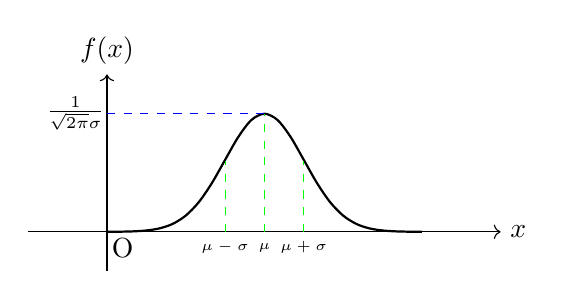
\begin{tikzpicture}
				\draw[->] (-1,0) -- (5,0) node[right] {$x$};
				\draw[->] (0,-0.5) -- (0,2) node[above] {$f(x)$};
				\draw[thick, domain=0:4, smooth, variable=\x] plot ({\x},{1.5*(2.7)^(-2*(\x-2)^(2)});
				\node at (0.2,-0.2) {O};
				\draw[dashed,blue] (0,1.5) -- (2,1.5);
				\draw[dashed,green] (1.5,0) -- (1.5,0.9);
				\draw[dashed,green] (2,0) -- (2,1.5);
				\draw[dashed,green] (2.5,0) -- (2.5,0.9);
				\node at (1.5,-0.2) {\tiny{$\mu-\sigma$}};
				\node at (2,-0.2) {\tiny{$\mu$}};
				\node at (2.5,-0.2) {\tiny{$\mu+\sigma$}};
				\node at (-0.4,1.5) {\small{$\frac{1}{\sqrt{2\pi}\sigma}$}};
			\end{tikzpicture}	
		}
		\subfigure[分布函数]{
			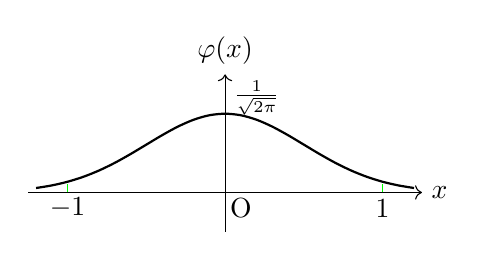
\begin{tikzpicture}
				\draw[->] (-2.5,0) -- (2.5,0) node[right] {$x$};
				\draw[->] (0,-0.5) -- (0,1.5) node[above] {$\varphi(x)$};
				\draw[thick, domain=-2.4:2.4, smooth, variable=\x] plot ({\x},{(2.71)^(-0.5*(\x)^(2)});
				\node at (0.2,-0.2) {O};
				\draw[dashed,green] (2,0) -- (2,0.137);
				\draw[dashed,green] (-2,0) -- (-2,0.137);
				\node at (-2,-0.2) {$-1$};
				\node at (2,-0.2) {$1$};
				\node at (0.4,1.2) {\small{$\frac{1}{\sqrt{2\pi}}$}};
			\end{tikzpicture}	
		}
	\end{figure}
\end{definition}
\section{一维随机变量函数的分布}
\begin{definition}
	设$X$是随机变量,函数$y=g(x)$,以随机变量$X$作为自变量的函数$Y=g(X)$也是随机变量,称为随机变量函数.
	
	我们一般有离散型$\rightarrow$离散型和连续型$\rightarrow$离散型两种随机变量函数.
\end{definition}
\chapterimage{chap23.jpg}
\chapter{多维随机变量及其分布}
\section{基本概念}
\begin{definition}[$n$维随机变量]
	如果$X_{1},X_{2},\cdots,X_{n}$是定义在同一个样本空间$\Omega$上的$n$个随机变量,我们称$(X_{1},X_{2},\cdots,X_{n})$为$n$维随机向量.
	
	对于任意的$n$个实数$x_{1},x_{2},\cdots,x_{n}$,我们把$n$元函数
	$$F(x_{1},x_{2},\cdots,x_{n})=P\{X_{1}\leq x_{1},X_{2}\leq x_{2},\cdots,X_{n}\leq x_{n}\}$$
	
	称为$n$维随机向量$(X_{1},X_{2},\cdots,X_{n})$的\textbf{联合分布函数}
	
	特别的,当$n=2$时,记$(X,Y)$为\textbf{二维随机变量}或者\textbf{二维随机向量},我们称$F(x,y)=P\{X\leq x,Y\leq y\}$为二维随机变量$(X,Y)$的联合分布函数,记作: 
	$$(X,Y)\sim F(x,y)\Leftrightarrow F(x,y)=P\{X\leq x,Y\leq y\}$$
	
	随机变量$X$与$Y$的分布函数$F_{X}(x)$和$F_{Y}(y)$分别称为随机变量关于$(X,Y)$关于$X$和$Y$的边缘分布函数.
	$$F_{X}(x)=P\{X\leq x\}=P\{X\leq x,Y< +\infty\}=F(x,+\infty)$$
	$$F_{Y}(y)=P\{Y\leq y\}=P\{X<+\infty,Y\leq y\}=F(+\infty,y)$$
	\begin{anymark}[注]
		\mathcolorbox{yellow}{\text{二维随机变量联合分布性质}}
		
		(1).单调性(单调不减)
		$$\forall x,\ \text{当}y_{1}<y_{2}\text{时},F(x,y_{1})\leq F(x,y_{2})$$
		$$\forall y,\ \text{当}x_{1}<x_{2}\text{时},F(x_{1},y)\leq F(x_{1},y)$$
		
		(2). 右连续性
		$$\lim\limits_{x\rightarrow x_{0}^{+}}F(x,y)=F(x_{0}+0,y)=F(x_{0},y)$$
		$$\lim\limits_{y\rightarrow y_{0}^{+}}F(x,y)=F(x,y_{0}+0)=F(x,y_{0})$$
		
		(3).有界性
		$$F(-\infty,y)=F(x,-\infty)=F(-\infty,-\infty)=0,\ F(+\infty,+\infty)=1$$
		
		(4).非负性
		$\forall x_{1}<x_{2},y_{1}<y_{2},\text{我们有}$: 
		$$F(x_{1}<x\leq x_{2},y_{1}<y\leq y_{2})=F(x_{2},y_{2})-F(x_{2},y_{1})-F(x_{1},y_{2})+F(x_{1},y_{1})\geq 0$$
	\end{anymark}
	
\end{definition}

\section{二维离散型随机变量}
\begin{table}[ht]
	\centering
	\caption{离散型二维随机变量概率分布}
	\label{table: 离散型二维随机变量概率分布}
	\begin{tblr}{
			hline{1,Z} = {2pt},
			hline{2,Y} = {1pt},
			vline{2,Y} = {1pt},
			cells = {$},
			cell{1}{1} = {mode = text}
	}
		\diagbox{$X$}{$Y$}                     & y_{1}  & \cdots & y_{j}  & \cdots & P\left\lbrace X=x_{i}\right\rbrace \\
		x_{1}                                  & p_{11} & \cdots & p_{1j} & \cdots & p_{1*}                             \\
		\vdots                                 & \vdots &        & \vdots &        & \vdots                             \\
		x_{i}                                  & p_{i1} & \cdots & p_{ij} & \cdots & p_{i*}                             \\
		\vdots                                 & \vdots &        & \vdots &        & \vdots                             \\
		P\left\lbrace Y=y_{j}\right\rbrace     & p_{*1} & \cdots & p_{*j} & \cdots & 1                                  \\
	\end{tblr}
\end{table}
\begin{definition}[二维离散型随机变量]
	\mathcolorbox{yellow}{\text{1.概率分布}}
	
	二维随机变量$(X,Y)$只能取有限对值或可列对值$(x_{1},y_{1}),(x_{2},y_{2}),\cdots,(x_{n},y_{n}),\cdots$,则称$(X,Y)$为离散型随机变量,$(X,Y)$满足概率分布: 
	$$p_{ij}=P\{X=x_{i},Y=y_{j}\},i,j=1,2,\cdots$$
	
	上面的式子称为$(X,Y)$的联合分布律,记作$(X,Y)\sim p_{ij}$,如 $\mathbf{table: }$ \ref{table: 离散型二维随机变量概率分布}所示
	
	$\text{数列}\{p_{ij}\},i,j=1,2,\cdots\text{是某一二维随机变量的概率分布的充要条件: }$
	$$ p_{ij}\geq 0,\ \sum\limits_{i=1}^{\infty}\sum\limits_{j=1}^{\infty}p_{ij}=1$$
	
	\mathcolorbox{yellow}{\text{2. 联合分布函数、边缘分布、条件分布}}
	
	(1). 联合分布函数
	$$F(x,y)=P\{X\leq x,Y\leq y\}=\sum\limits_{i=1}^{\infty}\sum\limits_{j=1}^{\infty}p_{ij}$$
	
	(2). 边缘分布
	
	$X$的边缘分布: 
	$$p_{i*}=P\{X=x_{i}\}=\sum\limits_{j=1}^{\infty}P\{X=x_{i},Y=y_{j}\}=\sum\limits_{j=1}^{\infty}p_{ij},(i=1,2,\cdots)$$
	$Y$的边缘分布: 
	$$p_{*j}=P\{Y=y_{j}\}=\sum\limits_{i=1}^{\infty}P\{X=x_{i},Y=y_{j}\}=\sum\limits_{i=1}^{\infty}p_{ij},(j=1,2,\cdots)$$
	
	(3). 条件分布
	
	$X$在$Y=y_{j}$下的条件分布: 
	$$P\{X=x_{i}|Y=y_{j}\}=\dfrac{P\{X=x_{i},Y=y_{j}\}}{P\{Y=y_{j}\}}=\dfrac{p_{ij}}{p_{*j}},i=1,2,\cdots$$
	$Y$在$X=x_{i}$下的条件分布: 
	$$P\{Y=y_{j}|X=x_{i}\}=\dfrac{P\{X=x_{i},Y=y_{j}\}}{P\{X=x_{i}\}}=\dfrac{p_{ij}}{p_{i*}},j=1,2,\cdots$$
\end{definition}
\section{二维连续型随机变量}
\begin{definition}[二维连续型随机变量]
	\mathcolorbox{yellow}{\text{1. 联合分布函数、概率密度}}
	$$F(x,y)=\int_{-\infty}^{x}\int_{-\infty}^{y}f(u,v)dudv,(x,y)\in\mathbb{R}^2$$
	
	$F(x,y)$是二维随机变量$(X,Y)$的概率分布函数,$f(x)$是二维随机变量$(X,Y)$的概率密度函数.
	
	$$f(x,y)\geq 0,\ \int_{-\infty}^{+\infty}\int_{-\infty}^{+\infty}f(x,y)dxdy$$
	\begin{anymark}[注]
		\begin{itemize}
			\item $f(x,y)$在点$(x_{0},y_{0})$处连续,我们有: $\dfrac{\partial^2 F(x,y)}{\partial x\partial y}|_{(x_{0},y_{0})}=f(x_{0},y_{0})$
			
			\item $F(x,y)$连续且可导,$\dfrac{\partial^2 F(x,y)}{\partial x\partial y}=f(x,y)$
		\end{itemize}
	\end{anymark}
	\mathcolorbox{yellow}{\text{2. 边缘分布函数、边缘概率密度}}
	
	$(X,Y)\sim f(x,y)$,$X$的边缘分布函数和边缘概率密度: 
	
	\mathcolorbox{orange}{\text{边缘分布函数}}
	\begin{flalign*}
		 F_{X}(x)=F(x,+\infty)=\int_{-\infty}^{x}\left[ \int_{-\infty}^{+\infty}f(u,v)dv\right] du
	\end{flalign*}
	
	\mathcolorbox{orange}{\text{边缘概率密度}}
	\begin{flalign*}
		f_{X}(x)=\int_{-\infty}^{+\infty}f(x,y)dy
	\end{flalign*}
	
	$(X,Y)\sim f(x,y)$,$Y$的边缘分布函数和边缘密度函数: 
	
	\mathcolorbox{orange}{\text{边缘分布函数}}
	\begin{flalign*}
		 F_{Y}(y)=F(+\infty,y)=\int_{-\infty}^{y}\left[ \int_{-\infty}^{+\infty}f(u,v)du\right] dv
	\end{flalign*}
	
	\mathcolorbox{orange}{\text{边缘概率密度}}
	\begin{flalign*}
		f_{Y}(y)=\int_{-\infty}^{+\infty}f(x,y)dx
	\end{flalign*}
	
	\mathcolorbox{orange}{\text{3. 条件分布函数、条件概率密度}}
	
	$(X,Y)\sim f(x,y)$,$X$在$Y=y$条件下的条件分布函数和条件概率密度: 
	
	\mathcolorbox{orange}{\text{条件概率密度}}
	\begin{flalign*}
	 f_{X|Y}(x|y)=\dfrac{f(x,y)}{f_{Y}(y)},(f_{Y}(y)>0)
	\end{flalign*}
	
	\mathcolorbox{orange}{\text{条件分布函数}}
	\begin{flalign*}
	 F_{X|Y}(x|y)=\int_{-\infty}^{x}f_{X|Y}(x|y)dx=\int_{-\infty}^{x}\dfrac{f(x,y)}{f_{Y}(y)}dx
	\end{flalign*}

	$(X,Y)\sim f(x,y)$,$Y$在$X=x$条件下的条件分布函数和条件概率密度: 
	
	\mathcolorbox{orange}{\text{条件概率密度}}
	\begin{flalign*}
	 f_{Y|X}(y|x)=\dfrac{f(x,y)}{f_{X}(x)},(f_{X}(x)>0)
	\end{flalign*}
	
	\mathcolorbox{orange}{\text{条件分布函数}}
	\begin{flalign*}
	 F_{Y|X}(y|x)=\int_{-\infty}^{y}f_{Y|X}(y|x)dy=\int_{-\infty}^{y}\dfrac{f(x,y)}{f_{X}(x)}dy
	\end{flalign*}
	
\end{definition}
\begin{definition}[常见二维分布]
	\mathcolorbox{skyblue}{\text{(1).二维均匀分布}}
	
	$(X,Y)$在有界区域$D$服从均匀分布,$(X,Y)$的概率密度为: 
	$$f(x,y)=\left\lbrace 
	\begin{array}{l}
		\dfrac{1}{S_{D}},\ (x,y)\in D\\
		0,\text{其他}
	\end{array}
	\right. S_{D}\text{是区域的面积}$$
	
	\mathcolorbox{skyblue}{\text{(2).二维正态分布}}
	
	$(X,Y)$概率密度为: 
	$$f(x,y)=\dfrac{1}{2\pi\sigma_{1}\sigma_{2}\sqrt{1-\rho^2}}exp\left\lbrace -\dfrac{1}{2(1-\rho^2)}\left[ \left( \dfrac{x-\mu_{1}}{\sigma_{1}}\right)^2-2\rho\left( \dfrac{x-\mu_{1}}{\sigma_{1}}\right)\left( \dfrac{x-\mu_{2}}{\sigma_{2}}\right) +\left( \dfrac{x-\mu_{2}}{\sigma_{2}}\right)^2\right] \right\rbrace $$
	
	其中$\mu_{1},\mu_{2}\in\mathbb{R},\ \sigma_{1},\sigma_{2}>0,-1<\rho<1$,我们称$(X,Y)$服从参数为$\mu_{1},\mu_{2},\sigma_{1},\sigma_{2},\rho$的二维正态分布,记作$(X,Y)\sim N(\mu_{1},\mu_{2};\sigma_{1}^2,\sigma_{2}^2;\rho)$
	
	\begin{anymark}[注]
		\begin{itemize}
			\item  $X\sim N(\mu_{1},\sigma_{1}^2)$,$Y\sim N(\mu_{2},\sigma_{2}^2)$,$\rho$是$X$与$Y$的相关系数
			$$\rho=\dfrac{Cov(X,Y)}{\sqrt{DX}\sqrt{DY}}=\dfrac{Cov(X,Y)}{\sigma_{1}\sigma_{2}}$$
			\item $X$和$Y$的条件分布都是正态分布
			\item $aX+bY(a\neq 0\text{或者}b\neq 0)$服从正态分布
			\item $X,Y$相互独立的充要条件为$X,Y$不相关$\Leftrightarrow \rho=0$
		\end{itemize}
	\end{anymark}
\end{definition}
\section{独立性}
\begin{definition}[独立性]
	1.概念
	
	设二维随机变量$(X,Y)$的联合分布$F(x,y)$,边缘分布分别为$F_{X}(x)$和$F_{Y}(y)$,如果对任意实数$(x,y)$,我们都有: 
	$$F(x,y)=F_{X}(x)F_{Y}(y)\Leftrightarrow X\text{和}Y\text{相互独立}$$
	
	\begin{itemize}
		\item 随机变量$X_{1},X_{2},\cdots,X_{n}$相互独立$\Leftrightarrow F(x_{1},x_{1},\cdots,x_{n})=F(x_{1})\dots F(x_{2})\cdots F(x_{n})$
		\item $X_{1},X_{2},\cdots,X_{n}$相互独立,则其中任意$k(2\leq k\leq n)$个随机变量也相互独立
		\item 两个多维随机变量$(X_{1},X_{2},\cdots,X_{n})$与$(Y_{1},Y_{2},\cdots,Y_{m})$相互独立,我们有: 
		$$F(x_{1},x_{2},\cdots,x_{n},y_{1},y_{2},\cdots,y_{m})=F_{1}(x_{1},x_{2},\cdots,x_{n})\dots F_{2}(y_{1},y_{2},\cdots,y_{m})$$
		\item $(X,Y)$为独立的二维随机变量,边缘分布和条件分布相等,边缘概率密度与条件概率密度相等.$(P\{Y=y_{j}\}>0,\ P\{X=x_{i}\}>0)$
		$$P\{X=x_{i}|Y=y_{j}\}=P\{X=x_{i}\},\ P\{Y=y_{j}|X=x_{i}\}=P\{Y=y_{j}\}$$
		$$f_{X|Y}(x|y)=\dfrac{f(x,y)}{f_{Y}(y)}=f_{X}(x)(f_{Y}(y)>0),\ f_{Y|X}(y|x)=\dfrac{f(x,y)}{f_{X}(x)}=f_{Y}(y)(f_{X}(x)>0)$$
	\end{itemize}
\end{definition}
\begin{definition}[连续型多维随机变量函数的分布]
	$(X,Y)\sim f(x,y)$
	
	\mathcolorbox{skyblue}{\text{(1).和的分布}}
	\begin{figure}[H]
		\centering  %图片全局居中
		\subfigure[$X+Y$]{
			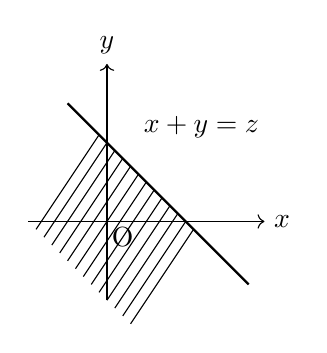
\begin{tikzpicture}
				\draw[->] (-1,0) -- (2,0) node[right] {$x$};
				\draw[->] (0,-1) -- (0,2) node[above] {$y$};
				\draw[thick, domain=-0.5:1.8, smooth, variable=\x] plot ({\x},{1-\x});
				\node at (0.2,-0.2) {O};
				\node at (1.2,1.2) {$x+y =z$};
				\foreach \i in {0,0.1,0.2,0.3,0.4,0.5,0.6,0.7,0.8,0.9,1,1.1,1.2}
				{
					\draw (\i-0.1,1.1-\i) -- (\i-0.9,-0.1-\i);
				}
			\end{tikzpicture}
		}
	\end{figure}
	$Z=X+Y$
	
	分布函数: 
	$$F_{Z}(z)=P\{X+Y\leq z\}=\iint\limits_{D_{z}:x+y\leq z}f(x,y)d\sigma=\left\lbrace 
	\begin{array}{l}
		\int_{-\infty}^{+\infty}dx\int_{-\infty}^{z-x}f(x,y)dy\\
		\int_{-\infty}^{+\infty}dy\int_{-\infty}^{z-y}f(x,y)dx
	\end{array}
	\right. $$
	
	概率密度: 
	$$f_{Z}(z)=F'_{Z}(z)=\left\lbrace 
	\begin{array}{l}
		\int_{-\infty}^{+\infty}f(z-y,y)dy\\
		\int_{-\infty}^{+\infty}f(x,z-x)dx
	\end{array}
	\right. $$
	
	\mathcolorbox{skyblue}{\text{(2).差的分布}}
	\begin{figure}[H]
		\centering  %图片全局居中
		\subfigure[$X-Y$]{
			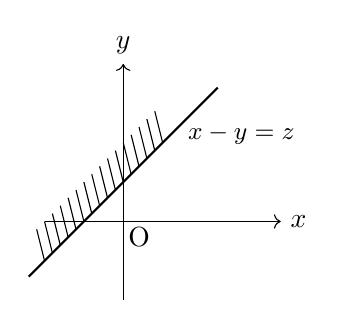
\begin{tikzpicture}
				\draw[->] (-1,0) -- (2,0) node[right] {$x$};
				\draw[->] (0,-1) -- (0,2) node[above] {$y$};
				\draw[thick, domain=-1.2:1.2, smooth, variable=\x] plot ({\x},{\x+0.5});
				\node at (0.2,-0.2) {O};
				\node at (1.5,1.1) {\small{$x-y =z$}};
				\foreach \i in {0,0.1,0.2,0.3,0.4,0.5,0.6,0.7,0.8,0.9,1,1.1,1.2,1.3,1.4,1.5}
				{
					\draw (\i-1,\i-0.5) -- (\i-1.1,\i-0.1);
				}
			\end{tikzpicture}	
		}
	\end{figure}
	$Z=X-Y$
	
	分布函数: 
	$$F_{Z}(z)=P\{X-Y\leq z\}=\iint\limits_{D_{z}:x-y\leq z}f(x,y)d\sigma=\left\lbrace 
	\begin{array}{l}
		\int_{-\infty}^{+\infty}dx\int_{x-z}^{+\infty}f(x,y)dy\\
		\int_{-\infty}^{+\infty}dy\int_{-\infty}^{y+z}f(x,y)dx
	\end{array}
	\right. $$
	
	概率密度: 
	$$f_{Z}(z)=F'_{Z}(z)=\left\lbrace 
	\begin{array}{l}
		\int_{-\infty}^{+\infty}f(z+y,y)dy\\
		\int_{-\infty}^{+\infty}f(x,x-z)dx
	\end{array}
	\right. $$
	
	\mathcolorbox{skyblue}{\text{(3).积的分布}}
	\begin{figure}[H]
		\centering  %图片全局居中
		\subfigure[$XY$]{
			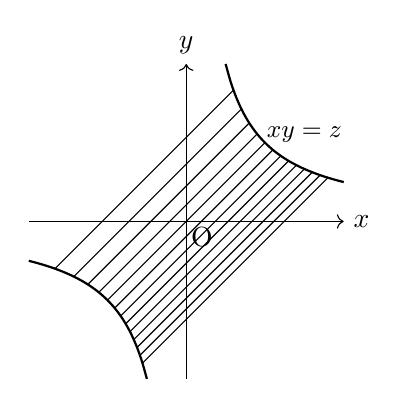
\begin{tikzpicture}
				\draw[->] (-2,0) -- (2,0) node[right] {$x$};
				\draw[->] (0,-2) -- (0,2) node[above] {$y$};
				\draw[thick, domain=0.5:2, smooth, variable=\x] plot ({\x},{1/\x});
				\draw[thick, domain=-2:-0.5, smooth, variable=\x] plot ({\x},{1/\x});
				\node at (0.2,-0.2) {O};
				\node at (1.5,1.1) {\small{$xy=z$}};
				\foreach \i in {0.6,0.7,0.8,0.9,1,1.1,1.2,1.3,1.4,1.5,1.6,1.7,1.8}
				{
					\draw (\i,1/\i) -- (-1/\i,-\i);
				}
			\end{tikzpicture}	
		}
	\end{figure}
	$Z=XY$
	
	分布函数: 
	\begin{eqnarray*}
		F_{Z}(z)&=&P\{XY\leq z\}=\iint\limits_{D_{z}:xy\leq z}f(x,y)d\sigma\\
		&=&\left\lbrace 
		\begin{array}{l}
			\int_{-\infty}^{0}dy\int_{\frac{z}{y}}^{+\infty}f(x,y)dx+\int_{0}^{+\infty}dy\int_{-\infty}^{\frac{z}{y}}f(x,y)dx\\
			\int_{-\infty}^{0}dx\int_{\frac{z}{x}}^{+\infty}f(x,y)dy+\int_{0}^{+\infty}dx\int_{-\infty}^{\frac{z}{x}}f(x,y)dy
		\end{array}
		\right.
	\end{eqnarray*}
	
	概率密度: 
	$$f_{Z}(z)=F'_{Z}(z)=\left\lbrace 
	\begin{array}{l}
		\int_{-\infty}^{0}(-\frac{1}{y})f(\frac{z}{y},y)dy+\int_{0}^{+\infty}\frac{1}{y}f(\frac{z}{y},y)dy=\int_{-\infty}^{+\infty}\frac{1}{|y|}f(\frac{z}{y},y)dy\\
		\int_{-\infty}^{0}(-\frac{1}{x})f(x,\frac{z}{x})dx+\int_{0}^{+\infty}\frac{1}{x}f(x,\frac{z}{x})dx=\int_{-\infty}^{+\infty}\frac{1}{|x|}f(x,\frac{z}{x})dx
	\end{array}
	\right. $$
	
	\mathcolorbox{skyblue}{\text{(4).商的分布}}
	\begin{figure}[H]
		\centering  %图片全局居中
		\subfigure[$\dfrac{X}{Y}$]{
			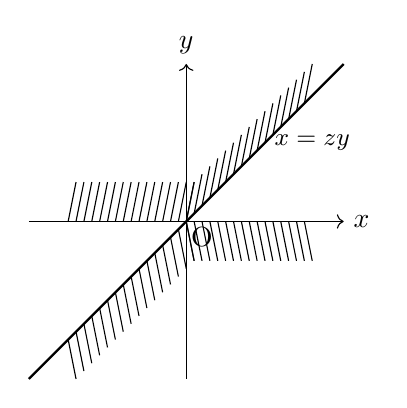
\begin{tikzpicture}
				\draw[->] (-2,0) -- (2,0) node[right] {$x$};
				\draw[->] (0,-2) -- (0,2) node[above] {$y$};
				\draw[thick, domain=-2:2, smooth, variable=\x] plot ({\x},{\x});
				\node at (0.2,-0.2) {O};
				\node at (1.6,1) {\small{$x=zy$}};
				\foreach \i in {0,0.1,0.2,0.3,0.4,0.5,0.6,0.7,0.8,0.9,1,1.1,1.2,1.3,1.4,1.5}
				{
					\draw (-\i,0) -- (-\i+0.1,0.5);
					\draw (\i,0) -- (\i+0.1,-0.5);
					\draw (\i,\i) -- (\i+0.1,\i+0.5);
					\draw (-\i,-\i) -- (-\i+0.1,-\i-0.5);
				}
			\end{tikzpicture}	
		}
	\end{figure}
	$Z=\dfrac{X}{Y}$
	
	分布函数: 
	$$F_{Z}(z)=P\{\dfrac{X}{Y}\leq z\}=\iint\limits_{D_{z}:\frac{X}{Y}\leq z}f(x,y)d\sigma=\int_{-\infty}^{0}dy\int_{zy}^{+\infty}f(x,y)dx+\int_{0}^{+\infty}dy\int_{-\infty}^{zy}f(x,y)dx$$
	
	概率密度: 
	$$f_{Z}(z)=F'_{Z}(z)=\int_{-\infty}^{0}(-y)f(zy,y)dy+\int_{0}^{+\infty}yf(zy,y)dy=\int_{-\infty}^{+\infty}|y|f(zy,y)dy$$
	
	\mathcolorbox{skyblue}{\text{(5).}max\{X,Y\}}
	
	$Z=max\{X,Y\}$
	
	分布函数: 
	\begin{eqnarray*}
		F_{Z}(z)=P\{Z\leq max\{X,Y\}\}&=&P\{X\leq z\}\cup P\{Y\leq z\}\\
		&=&P\{X\leq z\}+P\{Y\leq z\}-P\{X\leq z,Y\leq z\}\\
		&=&F_{X}(z)+F_{Y}(z)-F(z,z)
	\end{eqnarray*}

	
	概率密度: 
	$$f_{Z}=F'_{Z}(z)=f(z,z)$$
	
	\mathcolorbox{skyblue}{\text{(6).}min\{X,Y\}}
	
	$Z=min\{X,Y\}$
	
	分布函数: 
	$$F_{Z}(z)=P\{Z\leq min\{X,Y\}\}=P\{X\leq z,Y\leq z\}=F(z,z)\Rightarrow F_{max}(z)=F(z,z)$$
	
	概率密度: 
	$$f_{Z}=F'_{Z}(z)=f_{X}(z)+f_{Y}(z)-f(z,z)$$
	\begin{anymark}[注]
		\begin{itemize}
			\item  $n$个相互独立的随机变量$X_{1},X_{2},\cdots,X_{n}$,$Z_{1}=max\{X_{1},X_{2},\cdots,X_{n}\},\ Z_{2}=min\{X_{1},X_{2},\cdots,X_{n}\}$,$Z_{1},Z_{2}$的分布函数: 
			$$F_{max}(z)=F_{X_{1}}(z)F_{X_{2}}(z)\cdots F_{X_{n}}(z)$$
			$$F_{min}(z)=1-[1-F_{Z_{1}}(z)][1-F_{Z_{2}}(z)]\cdots[1-F_{Z_{n}}(z)]              $$
			\item $X_{i}(i=1,2,\cdots,n)$独立同分布,我们有: 
			$$F_{max}(x)=[F(x)]^n,\ f_{max}(x)=n[F(x)]^{n-1}f(x)$$
			$$F_{min}(x)=1-[1-F(x)]^n,\ f_{min}(x)=nf(x)[1-F(x)]^{n-1}$$
		\end{itemize}
	\end{anymark}
\end{definition}
\begin{table}[ht]
	\centering
	\caption{常见分布可加性}
	\label{table: 常见分布可加性}
	\begin{tblr}{
		hlines,
		vline{2,3},
		cells = {c,$}
	}
		X                       & Y                       & X+Y                                         \\
		B(n,p)                  & B(m,p)                  & B(n+m,p)                                    \\
		P(\lambda_{1})          & P(\lambda_{2})          & P(\lambda_{1}+\lambda_{2})                  \\
		N(\mu_{1},\sigma_{1}^2) & N(\mu_{2},\sigma_{2}^2) & N(\mu_{1}+\mu_{2},\sigma_{1}^2+\sigma_{2}^2)\\
		\chi^2(n)               & \chi^2(m)               & \chi^2(n+m)                                 \\
	\end{tblr}
\end{table}
\chapterimage{chap24.jpg}
\chapter{随机变量的数字特征}
\section{一维随机变量的数字特征}
\begin{definition}[数学期望]
		1. $X$是离散型随机变量,$X$的分布列为$p_{i}=P\{X=x_{i}\}(i=1,2,\cdots,n)$,如果级数$\sum\limits_{i=1}^{+\infty}x_{i}p_{i}$绝对收敛,我们称随机变量$X$的数学期望存在,并将其记作$E(X)$.
	$$E(X)=\sum\limits_{i=1}^{+\infty}x_{i}p_{i}$$
	
	2. $X$是连续型随机变量,$X$的概率密度为$f(x)$,如果积分$\int_{-\infty}^{+\infty}xf(x)dx$绝对收敛,我们称随机变量$X$的数学期望存在,并将其记作$E(X)$.
	$$E(X)=\int_{-\infty}^{+\infty}xf(x)dx$$
	\begin{itemize}
		\item  $a_{i}\text{为常数,}E\left(\sum\limits_{i=1}^{n}a_{i}X_{i} \right)=\sum\limits_{i=1}^{n}a_{i}E(X_{i}) $
		\item $E(X\pm Y)=E(X)\pm E(Y),\ E(aX+bY)=aE(X)+bE(Y)$
		\item $X\text{与}Y\text{相互独立}\Rightarrow E(XY)=E(X)E(Y),E\left[g_{1}(X)\dots g_{2}(Y) \right]=E\left[g_{1}(X)\right]\dots E\left[g_{2}(Y) \right] $
		\item $X_{1},X_{2},\cdots,X_{n}$相互独立,我们有: 
		$$E\left( \prod\limits_{i=1}^{n}X_{i}\right)=\prod\limits_{i=1}^{n}E(X_{i}),\ E\left[\prod\limits_{i=1}^{n}g_{i}(X_{i}) \right]=\prod\limits_{i=1}^{n}E\left[g_{i}(X_{i}) \right]   $$
	\end{itemize}
\end{definition}
\begin{definition}[方差和标准差]
	设$X$是随机变量,如果$E[(X-EX)^2]$存在,我们将$E[(X-EX)^2]$记作$X$的方差$D(X)(DX)$: 
	$$D(X)=E[(X-EX)^2]=E(X^2)-[E(X)]^2$$
	
	我们将$\sqrt{D(X)}$称为随机变量的\textbf{标准差}或者\textbf{均方差},记作$\sigma(X)$.
	\begin{itemize}
		\item $DX\geq 0,\ E(X^2)=DX+(EX)^2$
		\item $D(c)=0,\ c\text{为常数}$
		\item $D(aX+b)=a^2D(X),\ D(X+b)=D(X)$ 
		\item $D(X\pm Y)=D(X)+D(Y)\pm 2Cov(X,Y)$
		\item $X^{*}=\dfrac{X-E(X)}{\sigma(X)}$是$X$的标准化随机变量,$E(X^{*})=0,D(X^{*})=1$
		\item $\text{如果}X\text{和}Y\text{相互独立,我们得到}$
		$$D(aX+bY)=a^2D(X)+b^2D(Y)$$
		\item $X_{1},X_{2},\cdots,X_{n}$是相互独立,我们有: 
		$$D\left( \sum\limits_{i=1}^{n}a_{i}X_{i}\right)=\sum\limits_{i=1}^{n}a_{i}^2D(X_{i})$$
		$$D\left( \sum\limits_{i=1}^{n}g_{i}(X_{i})\right)=\sum\limits_{i=1}^{n}D\left[ g_{i}(X_{i})\right]  $$
	\end{itemize}
\end{definition}
\begin{definition}[切比雪夫不等式]
	如果随机变量$X$的期望$E(X)$和方差$D(X)$都存在,对任意$\varepsilon>0$,我们都有: 
	$$\mathcolorbox{purplea}{P\{|X-E(X)|\geq \varepsilon\}\leq \dfrac{D(X)}{\varepsilon^2}\text{或者}P\{|X-E(X)|< \varepsilon\}\geq 1-\dfrac{D(X)}{\varepsilon^2}}$$
	\begin{anymark}[注]
		
	\end{anymark}
\end{definition}

\section{二维随机变量的数字特征}
\begin{definition}[数学期望]
设 $X,Y$为随机变量,$g(X,Y)$为$X,Y$的函数($g$是连续函数)

1. $(X,Y)$是离散型随机变量,联合分布为: 
$$p_{ij}=P\{X=x_{i},Y=y_{j}\}(i,j=1,2,\cdots)$$

级数$\sum\limits_{i}\sum\limits_{j}g(x_{i},y_{j})p_{ij}$绝对收敛,我们定义: 
$$E[g(X,Y)]=\sum\limits_{i}\sum\limits_{j}g(x_{i},y_{j})p_{ij}$$

2. $(X,Y)$是连续型随机变量,概率密度为$f(x,y)$,积分$\int_{-\infty}^{+\infty}\int_{-\infty}^{+\infty}f(x,y)dxdy$绝对收敛,我们定义: 
$$E[g(X,Y)]=\int_{-\infty}^{+\infty}\int_{-\infty}^{+\infty}f(x,y)dxdy$$
\end{definition}
\begin{definition}[协方差与相关系数]
如果随机变量$X$与$Y$的方差存在且$D(X)>0,D(Y)>0$,我们定义随机变量$X,Y$的协方差$Cov(X,Y)$: 

$$Cov(X,Y)=E[(X-E(X))(Y-E(Y))]=E(XY)-E(X)E(Y)$$

其中$E(XY)$: 
$$E(XY)=\left\lbrace 
\begin{array}{l}
\sum\limits_{i}\sum\limits_{j}x_{i}y_{i}p_{ij},\ (X,Y)\text{是离散型随机变量}\\
\int_{-\infty}^{+\infty}\int_{-\infty}^{+\infty}xyf(x,y)dxdy,\ (X,Y)\text{是连续型随机变量}
\end{array}
\right. $$
	
我们将$\rho_{XY}=\dfrac{Cov(X,Y)}{\sqrt{DX}\sqrt{DY}}$定义为随机变量$X,Y$的\textbf{相关系数}.
\begin{itemize}
	\item $\rho_{XY}=0\Rightarrow X,Y\text{不相关}$
	\item $\rho_{XY}\neq0\Rightarrow X,Y\text{相关}$
	\item $\text{对称性}\  Cov(X,Y)=Cov(Y,X),\ Cov(X,X)=D(X),\ \rho_{XX}=1$
	\item $\text{线性} \ Cov(aX+b,Y)=aCov(X,Y),\ Cov(X_{1}+X_{2},Y)=Cov(X_{1},Y)+Cov(X_{2},Y)$
\end{itemize}
\end{definition}

\begin{table}[ht]
	\centering
	\caption{常用分布表}
	\label{table: 常用分布表}
	\begin{tblr}{
		hlines = {1pt},
		hline{1,Z} = {2pt},
		vline{2-Y} = {1pt},
		cells = {c}
	}
		$\text{名称}$                                    & $\text{概率分布}$                                                                    & $\text{均值}$            & $\text{方差}$                      & $\text{参数范围}$                       \\
		$\text{两点分布}$                                & {$P(X=k)=p^kq^{1-k}$\\ $(k=0,1)$}                                                   & $p$                      & $pq$                              & {$0<p<1$\\ $q=1-p$}                     \\
		{$\text{二项分布}$\\ $B(n,p)$}                   & {$P(X=k)=C_{n}^{k}p^xq^{n-k}$ \\ $(x=0,1,\cdots,n)$}                                & $np$                     & $npq$                             & {$0<p<1$ \\ $q=1-p$\\ $n\in N$}         \\
		{$\text{泊松分布}$\\ $P(\lambda$)}               & {$P(X=k)=\dfrac{\lambda^k}{k!}e^{-\lambda}$ \\ $(k=0,1,2,\cdots)$}                  & $\lambda$                & $\lambda$                         & $\lambda>0$                             \\
		{$\text{超几何分布}$\\ $H(n,N,M)$}               & {$P(X=k)=\dfrac{C_{N-M}^{n-k}C_{M}^{k}}{C_{N}^{n}}$\\ $(k=0,1,\cdots\,min\{M,n\})$} & $\dfrac{nM}{N}$          & $\dfrac{n(N-n)(N-M)M}{N^2(N-1)}$  & {$n,N,M\in N$\\ $n\leq N,M\leq N$}      \\
		{$\text{几何分布}$\\ $G(p)$}                     & {$P(X=k)=(1-p)^{k-1}p$\\ $(k=0,1,\cdots)$}                                          & $\dfrac{1}{p}$           & $\dfrac{1-p}{p^2}$                & {$0<p<1$\\ $q=1-p$}                     \\
		{$\text{均匀分布}$\\ $U(a,b)$}                   & $p(x)=\frac{1}{b-a}(a\leq x\leq b)$                                                 & $\dfrac{a+b}{2}$         & $\dfrac{(b-a)^3}{12}$             & {$0<p<1$\\ $q=1-p$\\ $r\in \mathbb{R}$} \\
		{$\text{指数分布}$\\ $E(\lambda)$}               & $p(x)=\lambda e^{-\lambda x}(x>0)$                                                  & $\dfrac{1}{\lambda}$     & $\dfrac{1}{\lambda^2}$            & $\lambda>0$                             \\
		{$\text{正态分布}$\\ $N(\mu,\sigma^2)$}          & $p(x)=\dfrac{1}{\sqrt{2\pi\sigma}}e^{-\dfrac{(x-\mu)^2}{2\sigma^2}}$                & $\mu$                    & $\sigma^2$                        & $\sigma>0$                              \\
		{$\Gamma\text{分布}$ \\ $\Gamma(\alpha,\beta)$} & $p(x)=\dfrac{\beta^{\alpha}}{\Gamma(\alpha)}x^{\alpha-1}e^{-\beta x}(x>0)$           & $\dfrac{\alpha}{\beta}$ & $\dfrac{\alpha}{\beta^2}$          & {$\alpha>0$\\ $\beta>0$}                \\
	\end{tblr}
\end{table}
\chapterimage{chap25.jpg}
\chapter{大数定理和中心极限定理}
\section{依概率收敛}
\begin{definition}[依概率收敛]
	设随机变量$X$与随机变量序列$\{X_{n}\}(n=1,2,3,\cdots)$,如果对于任意$\varepsilon>0$,我们有: 
	$$\lim\limits_{n\Rightarrow \infty}P\{|X_{n}-X|\geq \varepsilon\}=0\text{或者}\lim\limits_{n\Rightarrow \infty}P\{|X_{n}-X|<\varepsilon\}=1$$
	
	我们称随机变量序列$\{X_{n}\}$\textbf{依概率收敛于随机变量}$X$,记作: 
	$$\lim\limits_{n\Rightarrow \infty}X_{n}=X(P)\text{或者}X_{n}\stackrel{P}{\longrightarrow}X(n\Rightarrow \infty)$$
\end{definition}
\section{大数定理}
\begin{theorem}[切比雪夫大数定理]
	假设$\{X_{n}\}(n=1,2,\cdots)$是相互独立的随机变量序列,如果方差$D(X_{i})$存在且一致有上界,即存在常数$C$,$\forall i\geq 1, s.t. D(X_{i})\leq C$,$\{X_{n}\}$服从大数定理.
	$$\dfrac{1}{n}\sum\limits_{i=1}^{n}X_{i}\stackrel{P}{\longrightarrow}\dfrac{1}{n}\sum\limits_{i=1}^{n}E(X_{i})$$
\end{theorem}
\begin{theorem}[伯努利大数定理]
	假设$\mu_{n}$是$n$重伯努利试验中事件$A$发生的次数,在每次试验中事件$A$发生的概率为$p(0<p<1)$,则$\dfrac{\mu_{n}}{n}\stackrel{P}{\longrightarrow}p$.
	$$\forall \varepsilon>0,\lim\limits_{n\Rightarrow \infty}P\{|\dfrac{\mu_{n}}{n}-p|<\varepsilon\}=1$$
\end{theorem}
\begin{theorem}[辛钦大数定理]
	假设$\{X_{n}\}$是独立同分布的随机变量序列,如果$E(X_{i})=\mu,(i=1,2,\cdots)$存在,则$\dfrac{1}{n}\sum\limits_{i=1}^{n}X_{i}\stackrel{P}{\longrightarrow}\mu$.
	$$\forall \varepsilon>0,\lim\limits_{n\Rightarrow \infty}P\{|\dfrac{1}{n}\sum\limits_{i=1}^{n}X_{i}-\mu|<\varepsilon\}=1$$
\end{theorem}
\section{中心极限定理}
\begin{theorem}[列维-林德伯格定理]
	假设$\{X_{n}\}$是独立同分布的随机变量序列,如果$E(X_{i})=\mu,D(X_{i})=\sigma^2>0,(i=1,2,\cdots)$
	存在,$\forall x\in \mathbb{R}$,我们有: 
	$$\lim\limits_{n\Rightarrow \infty}P\{\dfrac{\sum\limits_{i=1}^{n}X_{i}-n\mu}{\sqrt{n\sigma}}<x\}=\dfrac{1}{\sqrt{2\pi}}\int_{-\infty}^{x}e^{-\frac{t^2}{2}}dt=\varPhi(x)$$
\end{theorem}
\begin{anymark}[注]
	\begin{itemize}
		\item $\text{定理满足}X_{n}\text{独立同分布、方差和期望存在}$
		\item $\sum\limits_{i=1}^{n}X_{i}\sim N(n\mu,n\sigma^2)$
		\item $P\{a<\sum\limits_{i=1}^{n}X_{i}<b\}\approx\varPhi(\dfrac{b-n\mu}{\sqrt{n}\sigma})-\varPhi(\dfrac{a-n\mu}{\sqrt{n}\sigma})$
	\end{itemize}
\end{anymark}
\begin{theorem}[棣莫弗-拉普拉斯定理]
	假设随机变量$Y_{n}\sim B(n,p),(0<p<1,n\geq 1)$,$\forall x\in \mathbb{R}$,我们有: 
	$$\lim\limits_{n\Rightarrow \infty}P\{\dfrac{Y_{n}-np}{\sqrt{np(1-p)}}<x\}=\dfrac{1}{\sqrt{2\pi}}\int_{-\infty}^{x}e^{-\frac{t^2}{2}}dt=\varPhi(x)$$
\end{theorem}
这一部分的内容我推荐一个$B$站视频观看.
\begin{itemize}
	\item \href{https://www.bilibili.com/video/BV1gh4y1W7ag/?spm_id_from=333.999.list.card_archive.click}{中心极限定理}
	\item \href{https://www.bilibili.com/video/BV1wu411W7uU/?spm_id_from=333.999.list.card_archive.click}{正态分布}
\end{itemize}
\chapterimage{chap26.jpg}
\chapter{数理统计}
\section{总体和样本}
\begin{definition}[统计概念和统计量]
	1. \textbf{总体}: 研究对象的全体称为总体
	
	2. \textbf{样本}: $n$个相互独立且与总体具有相同概率分布的随机变量$X_{1},X_{2},\cdots,X_{n}$所组成的整体$(X_{1},X_{2},\cdots,X_{n})$称为来自总体$X$,容量为$n$的一个\textbf{简单随机样本},一次抽样结果的具体的$n$个数值$(x_{1},x_{2},\cdots,x_{n})$称为样本$(X_{1},X_{2},\cdots,X_{n})$的一个观测值.
	
	3. \textbf{样本分布}
	
	假设总体的分布函数$F(x)$,概率密度函数$f(x)$,样本$(X_{1},X_{2},\cdots,X_{n})$的分布函数和概率密度: 
	$$\text{离散型: }P\{X_{1}=x_{1},X_{2}=x_{2},\cdots,X_{n}=x_{n}\}=\prod\limits_{i=1}^{n}P\{X_{i}=x_{i}\}$$
	$$\text{连续型分布函数: }F(x_{1},x_{2},\cdots,x_{n})=\prod\limits_{i=1}^{n}F(x_{i})$$
	$$\text{连续型概率密度: }f(x_{1},x_{2},\cdots,x_{n})=\prod\limits_{i=1}^{n}f(x_{i})$$
\end{definition}
\section{统计量及其分布}
\begin{definition}
	设$X_{1},X_{2},\cdots,X_{n}$是来自总体$X$的一个样本,$g(x_{1},x_{2},\cdots,x_{n})$是$n$元函数,如果函数$g$中不含任何参数,我们称$g(X_{1},X_{2},\cdots,X_{n})$是样本$X_{1},X_{2},\cdots,X_{n}$的一个\textbf{统计量}.
	
	1. \textbf{常用统计量}
	
	(1).数字特征
	\begin{itemize}
		\item \textbf{样本均值(一阶原点矩)}\ $\overline{X}=\dfrac{1}{n}\sum\limits_{i=1}^{n}X_{i}$
		\item \textbf{样本方差(二阶中心矩)}\ $S^2=\dfrac{1}{n-1}\sum\limits_{i=1}^{n}(X_{1}-\overline{X})^2$
		\item \textbf{样本}k\text{阶原点矩}\ $A_{k}=\dfrac{1}{n}\sum\limits_{i=1}^{n}X_{i}^{k},(k=1,2,\cdots)$
		\item \textbf{样本}k\text{阶中心矩}\ $B_{k}=\dfrac{1}{n}\sum\limits_{i=1}^{n}(X_{i}-\overline{X})^{k},(k=2,\cdots)$
	\end{itemize}
	
	(2). 顺序统计量
	
	将样本$X_{1},X_{2},\cdots,X_{n}$的$n$个观测值从小到大顺序排序得到: 
	$$X_{(1)}\leq X_{(2)}\leq \cdots\leq X_{(n)}\leq$$
	
	随机变量$X_{(k)}$称作第$k$顺序统计量,$X_{(1)}$为最小顺序统计量,$X_{(n)}$为最大顺序统计量.
	\begin{anymark}[注]
		假设总体期望$E(X)=\mu$,总体方差为$D(X)=\sigma^2$,$X_{1},X_{2},\cdots,X_{n}$是取自总体的一个样本,$\overline{X},S^2$分别为样本的均值和方差,我们有: 
		
		1.$E(X_{i})=\mu$
		
		2.$D(X_{i})=\sigma^2$
		
		3.$E(\overline{X})=E(\dfrac{X_{1}+X_{2}+\cdots+X_{n}}{n})=E(X)=\mu$
		
		4.$E(S^2)=D(X)=\sigma^2$
		
		5.$D(\overline{X})=\dfrac{1}{n}D(X)=\dfrac{\sigma^2}{n}$
	\end{anymark}
\end{definition}
\begin{definition}[三大分布]
	1. $\chi^2$分布
	
	随机变量$X_{1},X_{2},\cdots,X_{n}$相互独立,且都服从标准正态分布,则随机变量$X=\sum\limits_{i=1}^{n}X_{i}^2$服从自由度为$n$的卡方分布$\chi^2(n)$,记作$X\sim \chi^2(n)$.
	
	$\alpha$分位点: $\text{对于给定的}\alpha(0<\alpha<1),\text{满足}$
	$$P\{\chi^2>\chi_{\alpha}^2(n)\}=\int_{\chi_{\alpha}^2(n)}^{+\infty}f(x)dx$$
	的$\chi_{\alpha}^2(n)$为$\chi^2(n)$分布上的$\alpha$分位点.
	\begin{itemize}
		\item $X_{1}\sim \chi^2(n_{1}),\ X_{2}\sim \chi^2(n_{2})$,$X_{1},X_{2}$相互独立,我们有: $X_{1}+X_{2}\sim \chi^2(n_{1}+n_{2})$
		\item $X\sim \chi^2(n)\Rightarrow E(X)=n,D(X)=2n$
	\end{itemize}
	2. $t$分布
	
	设随机变量$X\sim N(0,1)$,$Y\sim \chi^2(n)$,$X,Y$相互独立,记随机变量$t=\dfrac{X}{\sqrt{Y/n}}$服从自由度为$n$的$t$分布,记作$t\sim t(n)$
	
	\begin{itemize}
		\item $t_{1-\alpha}(n)=-t_{\alpha}(n)$
		\item $t$分布概率密度关于$x$轴对称
	\end{itemize}
	
	3. $F$分布
	
	设随机变量$X\sim \chi^2(n_{1}),Y\sim \chi^2(n_{2})$,且$X,Y$相互独立,则$F=\dfrac{X/n_{1}}{Y/n_{2}}$服从自由度为$(n_{1},n_{2})$的$F$分布,记作$F\sim F(n_{1},n_{2})$.
	
	\begin{itemize}
		\item $F\sim F(n_{1},n_{2})\Rightarrow \dfrac{1}{F}\sim F(n_{2},n_{1})$
		\item $F_{1-\alpha}(n_{1},n_{2})=\dfrac{1}{F_{\alpha}(n_{2},n_{1})}$
	\end{itemize}
\end{definition}
\begin{anymark}[注]
	正态总体条件下常见结论: 
	
	设$X_{1},X_{2},\cdots,X_{n}$是来自正态总体$N(\mu,\sigma^2)$的一个样本,$\overline{X},S^2$分别是样本的均值和方差.
	
	1. $\overline{X}\sim N(\mu,\dfrac{\sigma^2}{n})\Rightarrow \dfrac{\overline{X}-\mu}{\frac{\sigma}{\sqrt{n}}}=\dfrac{\sqrt{n}(\overline{X}-\mu)}{\sigma}\sim N(0,1)$
	
	2. $\dfrac{1}{\sigma^2}\sum\limits_{i=1}^{n}(X_{i}-\mu)^2\sim \chi^2(n)$
	
	3. $\dfrac{(n-1)S^2}{\sigma^2}=\sum\limits_{i=1}^{n}(\dfrac{X_{i}-\overline{X}}{\sigma})^2\sim \chi^2(n)$
	
	4. $\overline{X}$和$S^2$相互独立,$\dfrac{\sqrt{n}(\overline{X}-\mu)}{S}\sim t(n-1)$
	
	5. $\sigma\text{未知时}$: $\dfrac{n(\overline{X}-\mu)^2}{S^2}\sim F(1,n-1)$
\end{anymark}
\section{参数的点估计}
\begin{definition}[矩估计和最大似然估计]
	1. 概念
	
	设总体$X$的分布函数$F(x,\theta)$,其中$\theta$是一个未知参数,$X_{1},X_{2},\cdots,X_{n}$是来自总体的一个样本,由样本构造一个适当的统计量$\hat{\theta}(X_{1},X_{2},\cdots,X_{n})$作为参数$\theta$的估计,称统计量为参数的估计量,$\theta=\hat{\theta}(X_{1},X_{2},\cdots,X_{n})$.
	
	2. 矩估计法
	
	设总体分布中有$k$个未知的参数$\theta_{1},\theta_{2},\cdots,\theta_{k}$,来自总体$X$的一组样本$X_{1},X_{2},\cdots,X_{n}$,如果$X$的原点矩$E(X^{l})(l=1,2,\cdots,k)$存在,我们令样本的原点矩=总体原点矩: 
	$$\dfrac{1}{n}\sum\limits_{i=1}^{n}X_{i}^{l}=E(X^{l})=\left\lbrace 
	\begin{array}{l}
		\int_{-\infty}^{+\infty}x^{l}f(x;\theta_{1},\theta_{2},\cdots,\theta_{k})dx\\
		\sum\limits_{i=1}^{n}x_{i}^{l}P\{X=x_{i};\theta_{1},\theta_{2},\cdots,\theta_{k}\}
	\end{array}
	\right. $$
	
	3. 最大似然估计法
	对未知参数$\theta$进行估计,在该参数可能的取值范围$I$中选取,使用使样本观测值$x_{1},x_{2},\cdots,x_{n}$最大的参数$\hat{\theta}$作为参数$\theta$的估计值.
	
	(1).总体$X$是离散型分布,分布函数的参数为$\theta_{1},\theta_{2},\cdots,\theta_{k}$,样本$X_{1},X_{2},\cdots,X_{n}$出现取值$x_{1},x_{2},\cdots,x_{n}$的概率为: 
	$$P\{X_{1}=x_{1},X_{2}=x_{2},\cdots,X_{n}=x_{n}\}=\prod\limits_{i=1}^{n}P(X_{i}=x_{i})=\prod\limits_{i=1}^{n}p(x_{i};\theta)$$
	
	我们得到似然函数: 
	$$L(\theta)=L(x_{1},x_{2},\cdots,x_{n},\theta)$$
	
	$$\exists \hat{\theta}\in I,\ s.t. L(x_{1},x_{2},\cdots,x_{n},\hat{\theta})=max_{\theta\in I}L(x_{1},x_{2},\cdots,x_{n},\theta)$$
	
	(2).总体$X$是连续型分布,概率密度为$f(x;\theta),\theta\in I$,样本$X_{1},X_{2},\cdots,X_{n}$出现取值$x_{1},x_{2},\cdots,x_{n}$的概率为: 
	$$L(\theta)=L(x_{1},x_{2},\cdots,x_{n},\theta)=\prod\limits_{i=1}^{n}f(x_{i},\theta)$$
	
	$$\exists \hat{\theta}\in I,\ s.t. L(x_{1},x_{2},\cdots,x_{n},\hat{\theta})=max_{\theta\in I}L(x_{1},x_{2},\cdots,x_{n},\theta)$$
	
	我们得到了参数的最大似然估计$\hat{\theta}=\hat{\theta}(x_{1},x_{2},\cdots,x_{n})$
	\begin{anymark}[估计量的评判标准]
		1. 无偏性
		
		2. 有效性(最小方差性)
		
		3. 一致性(相和性)
	\end{anymark}
\end{definition}
\section{参数的区间估计}
\begin{definition}[概念]
	设$\theta$是总体$X$的一个未知参数,对于给定的$\alpha(0<\alpha<1)$,如果由样本$X_{1},X_{2},\cdots,X_{n}$确定的两个统计量$\hat{\theta_{1}}=\hat{\theta_{1}}(X_{1},X_{2},\cdots,X_{n})$和$\hat{\theta_{2}}=\hat{\theta_{2}}(X_{1},X_{2},\cdots,X_{n})$满足: 
	$$P\{\hat{\theta_{1}}(X_{1},X_{2},\cdots,X_{n})<\theta<\hat{\theta_{2}}(X_{1},X_{2},\cdots,X_{n})\}=1-\alpha$$
	
	则称随机区间$(\hat{\theta_{1}},\hat{\theta_{2}})$是$\theta$的置信度为$1-\alpha$的\textbf{置信区间},$\hat{\theta_{1}}$和$\hat{\theta_{2}}$分别称为\textbf{置信上限}和\textbf{置信下限},$1-\alpha$为置信水平,$\alpha$为显著性水平.
\end{definition}
\begin{table}[h]
	\centering
	\caption{正态总体均值的置信区间}
	\label{table: 正态总体均值的置信区间}
	\begin{tblr}{
		hline{1,Z} = {2pt},
		hline{2,Y} = {1pt},
		vline{2-Y} = {1pt},
		cells = {c,$}
	}
		\text{待估参数} & \text{其他参数}     & \text{枢轴量分布}                                        & \text{置信区间}                                                                                                 \\
		\mu            & \sigma^2\text{已知} & Z=\dfrac{\overline{X}-\mu}{\sigma/\sqrt{n}}\sim N(0,1) & \left( \overline{X}-\frac{\sigma}{\sqrt{n}}z_{\alpha/2},\overline{X}+\frac{\sigma}{\sqrt{n}}z_{\alpha/2}\right) \\
		\mu            & \sigma^2\text{未知} & t=\dfrac{\overline{X}-\mu}{S/\sqrt{n}}\sim t(n-1)      & \left( \overline{X}-\frac{S}{\sqrt{n}}t_{\alpha/2}(n-1),\overline{X}+\frac{S}{\sqrt{n}}t_{\alpha/2}(n-1)\right) \\
	\end{tblr}
\end{table}
\section{假设检验}
\begin{definition}[统计性检验]
	1. $H_{0}\text{: 虚无假设},\ H_{1}\text{: 备择假设}$
	
	2. 双边检验和单侧检验
	
	3. 正态总体下的六大检查和拒绝域
	\begin{itemize}
		\item $\sigma^2\text{已知},\mu\text{未知},H_{0}\text{: }\mu=\mu_{0},H_{1}\text{: }\mu\neq \mu_{0}$
		$$\text{拒绝域: }(-\infty,\mu_{0}-\frac{\sigma}{\sqrt{n}}z_{\frac{\alpha}{2}})\cup (\mu_{0}+\frac{\sigma}{\sqrt{n}}z_{\frac{\alpha}{2}},+\infty)$$
		\item $\sigma^2\text{未知},\mu\text{未知},H_{0}\text{: }\mu=\mu_{0},H_{1}\text{: }\mu\neq \mu_{0}$
		$$\text{拒绝域: }(-\infty,\mu_{0}-\frac{S}{\sqrt{n}}t_{\frac{\alpha}{2}}(n-1))\cup (\mu_{0}+\frac{S}{\sqrt{n}}t_{\frac{\alpha}{2}}(n-1),+\infty)$$
		\item $\sigma^2\text{已知},\mu\text{未知},H_{0}\text{: }\mu\leq \mu_{0},H_{1}\text{: }\mu> \mu_{0}$
		$$\text{拒绝域: } (\mu_{0}+\frac{\sigma}{\sqrt{n}}z_{\frac{\alpha}{2}},+\infty)$$
		\item $\sigma^2\text{已知},\mu\text{未知},H_{0}\text{: }\mu\geq \mu_{0},H_{1}\text{: }\mu< \mu_{0}$
		$$\text{拒绝域: }(-\infty,\mu_{0}-\frac{\sigma}{\sqrt{n}}z_{\frac{\alpha}{2}})$$
		\item $\sigma^2\text{未知},\mu\text{未知},H_{0}\text{: }\mu\leq \mu_{0},H_{1}\text{: }\mu> \mu_{0}$
		$$\text{拒绝域: } (\mu_{0}+\frac{S}{\sqrt{n}}t_{\frac{\alpha}{2}}(n-1),+\infty)$$
		\item $\sigma^2\text{未知},\mu\text{未知},H_{0}\text{: }\mu\geq \mu_{0},H_{1}\text{: }\mu< \mu_{0}$
		$$\text{拒绝域: }(-\infty,\mu_{0}-\frac{S}{\sqrt{n}}t_{\frac{\alpha}{2}}(n-1))$$
	\end{itemize}
\end{definition}
	\partsimage{part.png}
	\part{每日一题\Rmnum{1}}
	\chapterimage{chap27.jpg}
\chapter{January}
\section{Week \Rmnum{1}}

\hl{\textbf{\textit{January 1}}}

1. 已知 $f(x+1)$ 的定义域为$[0,a]$,($a>0$),求 $f(x)$ 定义域
\myspace{1}
\begin{solution}
	
	$f(x+1)$ 的定义域为$[0,a]$,则 $f(x)$ 的定义域为$[-1,a-1]$
\end{solution}
\myspace{1}

2. 已知 $f(x)=e^{x^{2}},f[\varphi(x)]=1-x$ 且 $\varphi(x)\geq 0$,求 $\varphi(x)$ 并求出定义域
\myspace{1}
\begin{solution}
	
	$f[\varphi(x)]=1-x\Rightarrow e^{\varphi^{2}(x)}=1-x$, 因此: $\varphi(x)=\sqrt{\ln (1-x)}, x\ge 1$
\end{solution}
\myspace{1}

3. 设 
	$$g(x)=
	\begin{cases}
		2-x,x\leq 0\\ x+2,x>0
	\end{cases}$$,$$f(x)=
	\begin{cases}
		x^{2},x< 0\\ -x,x\geq 0
	\end{cases}
	$$
求 $g[f(x)]$
\myspace{1}
\begin{solution}

	$$
	g[f(x)] = 
	\begin{cases}
		2+x^{2}, & x<0\\
		x+2, & x\geq 0
	\end{cases}
	$$
\end{solution}
\myspace{1}

4. 设函数 $$f(x)=
\begin{cases}
	1-2x^{2},x<-1\\
	x^{3},-1\leq x\leq 2\\
	12x-16,x>2
\end{cases}
$$
求 $f(x)$ 的反函数 $g(x)$ 的表达式
\myspace{1}
\begin{solution}
	$$
	g(x) = 
	\begin{cases}
		-\sqrt{\dfrac{1-x}{2}}, & x\in(-\infty,-1)\\
		\displaystyle{\sqrt[3]{x}}, & x\in[-1,8]\\
		\dfrac{x+16}{12}, & x\in(8,+\infty)
	\end{cases}
	$$
\end{solution}
\myspace{1}

5. 证明:定义在 $[-a,a]$ 上的任意一个函数 $f(x)$ 都可以表示为一个奇函数和一个偶函数之和
\myspace{1}
\begin{solution}

	令 $g(x)= \dfrac{f(x)+f(-x)}{2}\quad h(x)=\dfrac{f(x)-f(-x)}{2}$
	$$
	\begin{cases}
		g(-x)=\dfrac{f(-x)+f(x)}{2}=\dfrac{f(x)+f(-x)}{2}=g(x)\\
		h(-x)=\dfrac{f(-x)-f(x)}{2}=\dfrac{f(x)-f(-x)}{2}=-h(x)\\
		f(x) = g(x)+h(x)
	\end{cases}
	$$
	
	其中 $g(x)$ 是偶函数, $h(x)$ 是奇函数
\end{solution}
\myspace{1}

6. 判断函数 $f(x)=x\tan x\cdot e^{\sin x}$的奇偶性、单调性、周期性和有界性
\myspace{1}
\begin{solution}

	$f(x)$ 定义域为 $(-\dfrac{\pi}{2}+k\pi,\dfrac{\pi}{2}+k\pi),k\in \mathbb{Z}$, 关于原点对称
	
	(1). 奇偶性: $f(-x) = x\tan x\cdot e^{-\sin x}\neq -f(x),\quad f(-x)\neq f(x)$

	$f(x)$ 是非奇非偶函数

	(2). 单调性: $f'(x) = \tan x\cdot e^{\sin x}+x\sec^{2}x\cdot e^{\sin x}+x\tan x\cos x\cdot e^{\sin x}=e^{\sin x}\left[\tan x+x\sin x+x\sec^{2}x\right]$

	$f(x)$ 不是单调函数

	(3). 有界性: $x\in(-\dfrac{\pi}{2},\dfrac{\pi}{2})$ 时, $f(x) > \dfrac{x\tan x}{e}$, 函数 $g(x)=\frac{x\tan x}{e}$ 为无界函数

	$f(x)$ 是无界函数

	(4). 周期性: $f(x+2\pi) = (x+2\pi)\tan(x+2\pi)\cdot e^{\sin(x+2\pi)} = (x+2\pi)\tan x\cdot e^{\sin x} \neq f(x)$

	$f(x)$ 不是周期函数
\end{solution}
\myspace{1}

7. 函数 $f(x)=\dfrac{|x|\sin(x-2)}{x(x-1)(x-2)^{2}}$ 在下列哪个区间内有界

\begin{itemize}
	\item A. $(-1,0)$
	\item B. $(0,1)$
	\item C. $(1,2)$
	\item D. $(2,3)$
\end{itemize}
\myspace{1}
\begin{solution}

	(1). $x\to 0^{-}, f(x)\to -\dfrac{\sin 2}{4}; x\to 0^{+}, f(x)\to \dfrac{\sin 2}{4}$

	(2). $x\to 1^{-}, f(x)\to +\infty; x\to 1^{+}, f(x)\to -\infty$

	(3). $x\to 2^{-}, f(x)\to -\infty; x\to 2^{+}, f(x)\to \infty$

	$f(x)$ 在区间 $(-1,0)$ 有界
\end{solution}
\myspace{1}

\hl{\textbf{\textit{January 2}}}

1. 求$\lim\limits_{n\to\infty}\left[\sqrt{1+2+\cdots+n}-\sqrt{1+2+\cdots+(n-1)}\right]$
\myspace{1}
\begin{solution}

	\begin{align*}
		I = & \lim\limits_{n\to\infty}\left[\sqrt{1+2+\cdots+n}-\sqrt{1+2+\cdots+(n-1)}\right]\\
		  = & \lim\limits_{n\to\infty}\left[\sqrt{\dfrac{n(n+1)}{2}}-\sqrt{\dfrac{(n-1)n}{2}}\right]\\
		  = & \lim\limits_{n\to\infty}\dfrac{\left[\dfrac{n(n+1)}{2}-\dfrac{n(n-1)}{2}\right]}{\sqrt{\dfrac{n(n+1)}{2}}+\sqrt{\dfrac{(n-1)n}{2}}}\\
		  = & \lim\limits_{n\to\infty}\dfrac{n}{\sqrt{2}n}\\
		  = & \dfrac{1}{\sqrt{2}} 
	\end{align*}
\end{solution}
\myspace{1}

2. 求极限 $\lim\limits_{x\to-\infty}\dfrac{\sqrt{4x^{2}+x-1}+x+1}{\sqrt{x^{2}+\sin x}}$
\myspace{1}
\begin{solution}

	\begin{align*}
		I = & \lim\limits_{x\to-\infty}\dfrac{\sqrt{4x^{2}+x-1}+x+1}{\sqrt{x^{2}+\sin x}}\\
		  = & \lim\limits_{x\to-\infty}\dfrac{\sqrt{x^{2}(4+\dfrac{1}{x}-\dfrac{1}{x^{2}})}+x(1+\dfrac{1}{x})}{\sqrt{x^{2}(1+\dfrac{\sin x}{x^{2}})}}\\
		  = & \lim\limits_{x\to-\infty}\dfrac{\sqrt{4+\dfrac{1}{x}-\dfrac{1}{x^{2}}}-(1+\dfrac{1}{x})}{\sqrt{1+\dfrac{\sin x}{x^{2}}}}\\
		  = & 1
	\end{align*}
\end{solution}
\myspace{1}

\hl{\textbf{\textit{January 3}}}

1. 求极限 $\lim\limits_{x\to 0}\left(\dfrac{2+e^{\frac{1}{x}}}{1+e^{\frac{4}{x}}}+\dfrac{\sin x}{|x|}\right)$
\myspace{1}
\begin{solution}

	\begin{align*}
		I^{+} = & \lim\limits_{x\to 0^{+}}\left(\dfrac{2+e^{\frac{1}{x}}}{1+e^{\frac{4}{x}}}+\dfrac{\sin x}{|x|}\right)\\
		      = & \lim\limits_{x\to 0^{+}}\dfrac{2+e^{\frac{1}{x}}}{1+e^{\frac{4}{x}}}+\lim\limits_{x\to 0^{+}}\dfrac{\sin x}{x}\\
			  = & 0+1 = 1\\
		I^{-} = & \lim\limits_{x\to 0^{-}}\left(\dfrac{2+e^{\frac{1}{x}}}{1+e^{\frac{4}{x}}}+\dfrac{\sin x}{|x|}\right)\\
			  = & \lim\limits_{x\to 0^{-}}\dfrac{2+e^{\frac{1}{x}}}{1+e^{\frac{4}{x}}}-\lim\limits_{x\to 0^{-}}\dfrac{\sin x}{x}\\
			  = & 2-1 = 1\\
	\end{align*}
	综上所述, 原极限 $I =1$
\end{solution}
\myspace{1}

2. 求极限 $\lim\limits_{x\to+\infty}(\sqrt{x^{2}+x}-\sqrt{x^{2}-x})$
\myspace{1}
\begin{solution}

	\begin{align*}
		I = & \lim\limits_{x\to+\infty}(\sqrt{x^{2}+x}-\sqrt{x^{2}-x})\\
		  = & \lim\limits_{x\to+\infty}\dfrac{(\sqrt{x^{2}+x}-\sqrt{x^{2}-x})(\sqrt{x^{2}+x}+\sqrt{x^{2}-x})}{\sqrt{x^{2}+x}+\sqrt{x^{2}-x}}\\
		  = & \lim\limits_{x\to+\infty}\dfrac{x^{2}+x-(x^{2}-x)}{\sqrt{x^{2}+x}+\sqrt{x^{2}-x}}\\
		  = & \lim\limits_{x\to+\infty}\dfrac{2x}{\sqrt{x^{2}+x}+\sqrt{x^{2}-x}}\\
		  = & \lim\limits_{x\to+\infty}\dfrac{2}{\sqrt{1+\dfrac{1}{x}}+\sqrt{1-\dfrac{1}{x}}}\\
		  = & 1
	\end{align*}
\end{solution}
\myspace{1}

\hl{\textbf{\textit{January 4}}}

1. 求极限 $\lim\limits_{x\to 0}\dfrac{\sqrt{1+\tan x}-\sqrt{1+\sin x}}{x(1-\cos x)}$
\myspace{1}
\begin{solution}

	\begin{align*}
		I = & \lim\limits_{x\to 0}\dfrac{\sqrt{1+\tan x}-\sqrt{1+\sin x}}{x(1-\cos x)}\\
		  = & \lim\limits_{x\to 0}\dfrac{\sqrt{1+\tan x}-\sqrt{1+\sin x}}{x(1-\cos x)}\cdot \dfrac{\sqrt{1+\tan x}+\sqrt{1+\sin x}}{\sqrt{1+\tan x}+\sqrt{1+\sin x}}\\
		  = & \lim\limits_{x\to 0}\dfrac{1+\tan x-1-\sin x}{x(1-\cos x)(\sqrt{1+\tan x}+\sqrt{1+\sin x})}\\
		  = & \lim\limits_{x\to 0}\dfrac{\tan x-\sin x}{x(1-\cos x)(\sqrt{1+\tan x}+\sqrt{1+\sin x})}\\
		  = & \lim\limits_{x\to 0}\dfrac{\dfrac{1}{2}x^{3}}{\dfrac{1}{2}x^{3}(\sqrt{1+\tan x}+\sqrt{1+\sin x})}\\
		  = & \dfrac{1}{2}
	\end{align*}
\end{solution}
\myspace{1}

2. 已知 $\lim\limits_{x\to 0}\dfrac{e^{x^{2}}-\cos 2x}{ax^{b}}=1$,求 $a,b$
\myspace{1}
\begin{solution}

	泰勒展开式:
	\begin{align*}
		I = & \lim\limits_{x\to 0}\dfrac{e^{x^{2}}-\cos 2x}{ax^{b}}\\
		  = & \lim\limits_{x\to 0}\dfrac{1+x^{2}+\dfrac{x^{4}}{2}-1+\dfrac{4x^{2}}{2!}-\dfrac{8x^{4}}{4!}}{ax^{b}}\\
		  = & \lim\limits_{x\to 0}\dfrac{3x^{2}-\dfrac{x^{4}}{6}}{ax^{b}}\\
		  = & \lim\limits_{x\to 0}\dfrac{3}{a} = 1
	\end{align*}
	因此: $a = 3, b = 2$
\end{solution}
\myspace{1}

\hl{\textbf{\textit{January 5}}}

1. 已知 $\lim\limits_{x\to x_{0}}\varphi(x)=0$,下列结论正确的个数为
\begin{itemize}
	\item A. $\lim\limits_{x\to x_{0}}\dfrac{\sin\varphi(x)}{\varphi(x)}=1$
	\item B. $\lim\limits_{x\to x_{0}}[1+\varphi(x)]^{\frac{1}{\varphi}}=e$
	\item C. 当$x\to x_{0}$时,$\sin \varphi(x)\sim \varphi(x)$
	\item D. 若$\lim\limits_{u\to 0}f(u)=A$,则 $\lim\limits_{x\to x_{0}}f[\varphi(x)]=A$
\end{itemize}
\myspace{1}
\begin{solution}

	正确的个数: $0$, 令 $\varphi(x) = 0,x\in \mathring{U}(x_{0},\delta)$, $A,B,C,D$ 四个选项均不正确
\end{solution}
\myspace{1}

2. 求极限 $\lim\limits_{x\to 0}\dfrac{\arcsin x-\arctan x}{\sin x-\tan x}$
\myspace{1}
\begin{solution}

	\begin{align*}
		I = & \lim\limits_{x\to 0}\dfrac{\arcsin x-\arctan x}{\sin x-\tan x}\\
		  = & \lim\limits_{x\to 0}\dfrac{\dfrac{1}{2}x^{3}}{-\dfrac{1}{2}x^{3}}\\
		  = & -1 
	\end{align*}
\end{solution}
\myspace{1}
\hl{\textbf{\textit{January 6}}}

1. 求极限 $\lim\limits_{x\to 0}\dfrac{\ln\dfrac{x}{\ln(1+x)}}{x}$
\myspace{1}
\begin{solution}

	\begin{align*}
		I = & \lim\limits_{x\to 0}\dfrac{\ln\dfrac{x}{\ln(1+x)}}{x}\\
		  = & \lim\limits_{x\to 0}\dfrac{x-\ln(1+x)}{x\ln (1+x)}\\
		  = & \lim\limits_{x\to 0}\dfrac{\dfrac{1}{2}x^{2}}{x^{2}}\\
		  = & \dfrac{1}{2}
	\end{align*}
\end{solution}
\myspace{1}

2. 求极限 $\lim\limits_{x\to +\infty}\dfrac{e^{x}}{(1+\dfrac{1}{x})^{x^{2}}}$
\myspace{1}
\begin{solution}
	
	\begin{align*}
		I = & \lim\limits_{x\to +\infty}\dfrac{e^{x}}{(1+\frac{1}{x})^{x^{2}}}\\
		  = & \lim\limits_{x\to +\infty}\dfrac{e^{x}}{e^{x^{2}\ln(1+\frac{1}{x})}}\\
		  = & \lim\limits_{x\to +\infty}e^{x-x^{2}\ln(1+\frac{1}{x})}\\
		  = & \lim\limits_{x\to +\infty}e^{x-x^{2}(\frac{1}{x}-\frac{1}{2x^{2}})}\\
		  = & \lim\limits_{x\to +\infty}e^{\frac{1}{2}}\\
		  = & e^{\frac{1}{2}}
	\end{align*}
\end{solution}
\myspace{1}
\hl{\textbf{\textit{January 7}}}

1. 求极限 $\lim\limits_{x\to 0}\dfrac{\cos x-\cos(\sin x)}{x^{4}}$
\myspace{1}
\begin{solution}

	\begin{align*}
		I = & \lim\limits_{x\to 0}\dfrac{\cos x-\cos(\sin x)}{x^{4}} (\text{Lagrange's Mean Value Theorem})\\
		  = & \lim\limits_{x\to 0}\dfrac{-\sin \xi(x-\sin x)}{x^{4}}, \xi\in (\sin x\sim x)\\
		  = & \lim\limits_{x\to 0}\dfrac{-\sin \xi}{6x}\\
		  = & -\dfrac{1}{6}
	\end{align*}

	夹逼定理: 
	$$\sin \xi \in (\sin x\sim x)\to \lim\limits_{x\to 0}\dfrac{\sin x}{x} = \lim\limits_{x\to 0}\dfrac{x}{x}=1\Rightarrow \lim\limits_{x\to 0}\dfrac{\sin \xi}{x} = 1$$

\end{solution}
\myspace{1}

2. 求极限 $\lim\limits_{x\to +\infty}x^{2}\left[\arctan(x+1)-\arctan x\right]$
\myspace{1}
\begin{solution}

	\begin{align*}
		I = & \lim\limits_{x\to +\infty}x^{2}[\arctan(x+1)-\arctan x](\text{Lagrange's Mean Value Theorem})\\
		  = & \lim\limits_{x\to +\infty}x^{2}\dfrac{1}{1+\xi^{2}},\xi\in(x,x+1)\\
		  = & 1
	\end{align*}

	夹逼定理: 
	$$\xi\in (x, x+1)\to \lim\limits_{x\to +\infty}\frac{x^{2}}{1+(x^{2})} = \lim\limits_{x\to +\infty}\frac{x^{2}}{1+(x+1)^{2}}=1
	\Rightarrow \lim\limits_{x\to +\infty}\frac{x^{2}}{1+\xi^{2}} = 1$$
\end{solution}
\myspace{1}

\section{Week \Rmnum{2}}
\hl{\textbf{\textit{January 8}}}

1. 求极限 $\lim\limits_{n\to \infty}n^{2}\left[\arctan\dfrac{a}{n}-\arctan \dfrac{a}{n+1}\right]$
\myspace{1}
\begin{solution}
	
	归结原理:
	\begin{align*}
		I = & \lim\limits_{x\to \infty}x^{2}[\arctan\dfrac{a}{x}-\arctan \dfrac{a}{x+1}](\text{Lagrange's Mean Value Theorem})\\
		  = & \lim\limits_{x\to \infty}\dfrac{ax^{2}}{x(x+1)}\dfrac{1}{1+\xi^{2}},\xi\in(\dfrac{a}{x},\dfrac{a}{x+1})\\
		  = & a
	\end{align*}

	夹逼定理: 
	$$\xi\in (\dfrac{a}{x},\dfrac{a}{x+1})\to \lim\limits_{x\to \infty}\dfrac{a}{x} = \lim\limits_{x\to \infty}\dfrac{a}{x+1}=0\Rightarrow \lim\limits_{x\to \infty}\xi = 0$$
\end{solution}
\myspace{1}

2. 求极限 $\lim\limits_{x\to +\infty}[\sin\sqrt{x+1}-\sin\sqrt{x}]$
\myspace{1}
\begin{solution}
	
	\begin{align*}
		I = & \lim\limits_{x\to +\infty}[\sin\sqrt{x+1}-\sin\sqrt{x}](\text{Lagrange's Mean Value Theorem})\\
		  = & \lim\limits_{x\to +\infty}\cos \xi(\sqrt{x+1}-\sqrt{x}),\xi\in(\sqrt{x},\sqrt{x+1})\\
		  = & \lim\limits_{x\to +\infty}\cos \xi(\dfrac{1}{\sqrt{x+1}+\sqrt{x}})\\
		  = & 0
	\end{align*}
\end{solution}
\myspace{1}

\hl{\textbf{\textit{January 9}}}

1. 求极限 $\lim\limits_{x\to 0}\left[\dfrac{1}{\ln(1+x^{2})}-\dfrac{1}{\ln(1+\tan^{2}x)}\right]$
\myspace{1}
\begin{solution}
	
	\begin{align*}
		I = & \lim\limits_{x\to 0}\left[\dfrac{1}{\ln(1+x^{2})}-\dfrac{1}{\ln(1+\tan^{2}x)}\right]\\
		  = & \lim\limits_{x\to 0}\dfrac{\ln(1+\tan^{2}x)-\ln(1+x^{2})}{\ln(1+x^{2})\ln(1+\tan^{2}x)}(\text{Lagrange's Mean Value Theorem})\\
		  = & \lim\limits_{x\to 0}\dfrac{(\tan x+x)(\tan x-x)}{x^{4}\xi}, \xi\in(1+x^{2},1+\tan^{2}x)\\
		  = & \lim\limits_{x\to 0}\dfrac{2x\cdot \dfrac{x^{3}}{3}}{x^{4}}\\
		  = & \dfrac{2}{3}
	\end{align*}

	夹逼定理: 
	$$\xi\in(1+x^{2},1+\tan^{2}x)\to \lim\limits_{x\to 0}(1+x^{2}) = \lim\limits_{x\to 0} (1+\tan^{2}x) = 1\Rightarrow \lim\limits_{x\to 0}\xi = 1$$
\end{solution}
\myspace{1}

2. 求极限 $\lim\limits_{x\to 0}\left[\dfrac{1}{\ln(1+x^{2})}-\dfrac{1}{\sin^{2}x}\right]$
\myspace{1}
\begin{solution}

	\begin{align*}
		I = & \lim\limits_{x\to 0}\left[\dfrac{1}{\ln(1+x^{2})}-\dfrac{1}{\sin^{2}x}\right]\\
		  = & \lim\limits_{x\to 0}\dfrac{\sin^{2}x-\ln(1+x^{2})}{\ln(1+x^{2})\sin^{2}x}\\
		  = & \lim\limits_{x\to 0}\dfrac{\sin^{2}x-x^{2}+x^{2}-\ln(1+x^{2})}{x^{4}}\\
		  = & \lim\limits_{x\to 0}\dfrac{\sin^{2}x-x^{2}}{x^{4}}+\lim\limits_{x\to 0}\dfrac{x^{2}-\ln(1+x^{2})}{x^{4}}\\
		  = & \lim\limits_{x\to 0}\dfrac{(\sin x+x)(\sin x-x)}{x^{4}}+\lim\limits_{x\to 0}\dfrac{\dfrac{1}{2}x^{4}}{x^{4}}\\
		  = & \dfrac{1}{2}+\lim\limits_{x\to 0}\dfrac{2x\cdot(-\dfrac{1}{6}x^{3})}{x^{4}}\\ 
		  = & \dfrac{1}{6}
	\end{align*}
	
	夹逼定理: 
	$$\xi\in(1+\sin^{2}x,1+x^{2})\to \lim\limits_{x\to 0}(1+\sin^{2}x) = \lim\limits_{x\to 0} (1+x^{2}) = 1\Rightarrow \lim\limits_{x\to 0}\xi = 1$$
\end{solution}
\myspace{1}
\hl{\textbf{\textit{January 10}}}

1. 求极限 $\lim\limits_{x\to 0}\left(x+2^{x}\right)^{\frac{2}{x}}$
\myspace{1}
\begin{solution}
	
	\begin{align*}
		I = & \lim\limits_{x\to 0}(x+2^{x})^{\frac{2}{x}}\\
		  = & \lim\limits_{x\to 0}e^{\frac{2\ln(x+2^{x})}{x}}\\
		  = & e^{\lim\limits_{x\to 0}\frac{2\ln(x+2^{x})}{x}}\\
		  = & e^{\lim\limits_{x\to 0}\frac{2(x+2^{x}-1)}{x}}\\
		  = & e^{\lim\limits_{x\to 0}\frac{2x}{x}+\lim\limits_{x\to 0}\frac{2x\ln 2}{x}}\\
		  = & e^{2+2\ln 2}\\
		  = & 4e^{2}
	\end{align*}
\end{solution}
\myspace{1}

2. 若 $\lim\limits_{x\to 0}\left(\dfrac{1-\tan x}{1+\tan x}\right)^{\frac{1}{\sin kx}}=e$,求 $k$
\myspace{1}
\begin{solution}
	
	\begin{align*}
		I = & \lim\limits_{x\to 0}\left(\dfrac{1-\tan x}{1+\tan x} \right)^{\frac{1}{\sin kx}} \\
		  = & \lim\limits_{x\to 0}e^{\frac{1}{\sin kx}\ln\frac{1-\tan x}{1+\tan x}}\\
		  = & e^{\lim\limits_{x\to 0}\frac{1}{\sin kx}\ln(1-\frac{2\tan x}{1+\tan x})}\\
		  = & e^{\lim\limits_{x\to 0}-\frac{2\tan x}{(1+\tan x)sin kx}}\\
		  = & e^{\lim\limits_{x\to 0}-\frac{2x}{kx}}\\
		  = & e^{-\frac{2}{k}} = e
	\end{align*}

	综上所述, $k = -2$
\end{solution}
\myspace{1}
\hl{\textbf{\textit{January 11}}}

1.  若 $\lim\limits_{x\to 0}(e^{x}+ax^{2}+bx)^{\frac{1}{x^{2}}}=1$,求 $a,b$
\myspace{1}
\begin{solution}

	\begin{align*}
		I = & \lim\limits_{x\to 0}(e^{x}+ax^{2}+bx)^{\frac{1}{x^{2}}}\\
		  = & \lim\limits_{x\to 0}e^{\frac{1}{x^{2}}\ln(e^{x}+ax^{2}+bx)}\\
		  = & e^{\lim\limits_{x\to 0}\frac{e^{x}+ax^{2}+bx-1}{x^{2}}}\quad (\text{Taylor's Formula})\\
		  = & e^{\lim\limits_{x\to 0}\frac{(a+\frac{1}{2})x^{2}+(b+1)x+o(x^{2})}{x^{2}}}\\
		  = & 1
	\end{align*}

	综上所述, $a = -\dfrac{1}{2}, b = -1$
\end{solution}
\myspace{1}

2. 求极限 $\lim\limits_{x\to 0}\left(\dfrac{\arctan x}{x}\right)^{\frac{1}{1-\cos x}}$
\myspace{1}
\begin{solution}
	
	\begin{align*}
		I = & \lim\limits_{x\to 0}\left(\dfrac{\arctan x}{x}\right)^{\frac{1}{1-\cos x}}\\
		  = & \lim\limits_{x\to 0}e^{\frac{1}{1-\cos x}\ln\frac{\arctan x}{x}}\\
		  = & e^{\lim\limits_{x\to 0}\frac{1}{1-\cos x}\ln\frac{\arctan x}{x}}\\
		  = & e^{\lim\limits_{x\to 0}\frac{1}{1-\cos x}\ln(1+\frac{\arctan x-x}{x})}\\
		  = & e^{\lim\limits_{x\to 0}\frac{1}{1-\cos x}\frac{\arctan x-x}{x}}\\
		  = & e^{\lim\limits_{x\to 0}-\frac{2x^{3}}{3x^{3}}}\\
		  = & e^{-\frac{2}{3}}
	\end{align*}
\end{solution}
\myspace{1}
\hl{\textbf{\textit{January 12}}}

1. 求极限 $\lim\limits_{n\to \infty}\left(n\tan\frac{1}{n}\right)^{n^{2}}$
\myspace{1}
\begin{solution}
	
	归结原理:
	\begin{align*}
		I = & \lim\limits_{x\to \infty}\left(x\tan\frac{1}{x}\right)^{x^{2}}\\
		  = & \lim\limits_{x\to \infty}e^{x^{2}\ln(x\tan\frac{1}{x})}\\
		  = & e^{\lim\limits_{x\to \infty}x^{2}\ln(x\tan\frac{1}{x})}\\
		  = & e^{\lim\limits_{t\to 0}\frac{\ln(\frac{\tan t}{t})}{t^{2}}}\\
		  = & e^{\lim\limits_{t\to 0}\frac{\tan t-t}{t^{3}}}\\
		  = & e^{\frac{1}{3}}
	\end{align*}
\end{solution}
\myspace{1}

2. 求极限 $\lim\limits_{n\to \infty}\tan^{n}\left( \dfrac{\pi}{4}+\dfrac{1}{n}\right)$
\myspace{1}
\begin{solution}
	
	归结原理:
	\begin{align*}
		I = & \lim\limits_{x\to \infty}e^{x\ln(\tan(\frac{\pi}{4}+\frac{1}{x}))}\\
		  = & \lim\limits_{x\to \infty}e^{x\ln(\frac{1+\tan(\frac{1}{x})}{1-\tan(\frac{1}{x})})}\\
		  = & \lim\limits_{t\to 0}e^{\frac{2\tan t}{t(1-\tan t)}}\\
		  = & e^{2}
	\end{align*}
\end{solution}
\myspace{1}
\hl{\textbf{\textit{January 13}}}

1. 求极限 $\lim\limits_{x\to 0}\left( \dfrac{\ln(1+x)}{x}\right)^{\frac{1}{e^{x}-1}}$
\myspace{1}
\begin{solution}

	\begin{align*}
		I = & \lim\limits_{x\to 0}e^{\frac{\ln(1+x)-x}{x(e^{x}-1)}}\\
		  = & e^{\lim\limits_{x\to 0}\frac{\ln(1+x)-x}{x^{2}}}\\
		  = & e^{\frac{1}{2}}
	\end{align*}
\end{solution}
\myspace{1}

2. 求极限 $\lim\limits_{x\to 0}\left( \dfrac{(1+x)^{\frac{1}{x}}}{e}\right)^{\frac{1}{x}}$
\myspace{1}
\begin{solution}

	\begin{align*}
		I = & \lim\limits_{x\to 0}e^{\frac{\ln(1+x)-x}{x^{2}}}\\
		  = & e^{\frac{1}{2}}
	\end{align*}
\end{solution}
\myspace{1}
\hl{\textbf{\textit{January 14}}}

1. 求极限 $\lim\limits_{x\to 0}(\cos 2x+2x\sin x)^{\frac{1}{x^{4}}}$
\myspace{1}
\begin{solution}

	\begin{align*}
		I = & \lim\limits_{x\to 0}e^{\frac{2x\sin x+\cos 2x-1}{x^{4}}}\quad (\text{Taylor's Formula})\\
		  = & e^{\lim\limits_{x\to 0}\frac{2x(x-\frac{x^{3}}{6})-2x^{2}+\frac{2}{3}x^{4}}{x^{4}}}\\
		  = & e^{\frac{1}{3}}
	\end{align*}
\end{solution}
\myspace{1}

2. 求极限 $\lim\limits_{x\to \frac{\pi}{4}}\left( \tan x\right) ^{\frac{1}{\cos x-\sin x}}$
\myspace{1}
\begin{solution}

	\begin{align*}
		I = & \lim\limits_{x\to \frac{\pi}{4}}e^{\frac{\tan x-1}{\cos x-\sin x}}\\
		  = & e^{\lim\limits_{x\to \frac{\pi}{4}}\frac{\tan x-1}{\cos x(1-\tan x)}}\\
		  = & e^{\lim\limits_{x\to \frac{\pi}{4}}-\frac{1}{\cos x}}\\
		  = & e^{-\sqrt{2}}
	\end{align*}
\end{solution}
\myspace{1}
\section{Week \Rmnum{3}}
\hl{\textbf{\textit{January 15}}}

1. 求极限 $\lim\limits_{x\to 0}\left(\dfrac{(e^{x}+e^{2x}+\cdots +e^{nx})}{n} \right)^{\frac{1}{x}} $
\myspace{1}
\begin{solution}

	\begin{align*}
		I = & \lim\limits_{x\to 0}e^{\frac{\ln \frac{e^{x}+e^{2x}+\cdots +e^{nx}}{n}}{x}}\\
		  = & e^{\lim\limits_{x\to 0}\frac{e^{x}-1+e^{2x}-1+\cdots +e^{nx}-1}{nx}}\\
		  = & e^{\lim\limits_{x\to 0}\frac{\frac{n(n+1)x}{2}}{nx}}\\
		  = & e^{\frac{n+1}{2}}
	\end{align*}
\end{solution}
\myspace{1}

2. 求极限 $\lim\limits_{x\to \infty}\left(\dfrac{x^{n}}{(x+1)(x+2)\cdots(x+n)} \right)^{x} $
\myspace{1}
\begin{solution}

	\begin{align*}
		I = & \lim\limits_{x\to +\infty}\left(1+\dfrac{1}{x}\right)^{-x}\left(1+\dfrac{2}{x}\right)^{-x}\cdots \left(1+\dfrac{n}{x}\right)^{-x}\\
		  = & e^{\lim\limits_{x\to +\infty}-x\ln(1+\frac{1}{x})}e^{\lim\limits_{x\to +\infty}-x\ln(1+\frac{2}{x})}\cdots e^{\lim\limits_{x\to +\infty}-x\ln(1+\frac{n}{x})}\\
		  = & e^{-1}e^{-2}\cdots e^{-n}\\
		  = & e^{-\frac{n(n+1)}{2}}
	\end{align*}
\end{solution}
\myspace{1}
\hl{\textbf{\textit{January 16}}}

1. 求极限 $\lim\limits_{x\to \infty}\left(\sin\frac{1}{x}+\cos\frac{1}{x} \right)^{x} $
\myspace{1}
\begin{solution}

	\begin{align*}
		I = & \lim\limits_{x\to \infty}\left(\sin\frac{1}{x}+\cos\frac{1}{x} \right)^{x}\\
		  = & e^{\lim\limits_{x\to +\infty}x\ln(\sin\frac{1}{x}+\cos\frac{1}{x})}\\
		  = & e^{\lim\limits_{t\to 0}\frac{\ln(\sin t+\cos t)}{t}}\\
		  = & e^{\lim\limits_{t\to 0}\frac{\sin t+\cos t-1}{t}}\\
		  = & e
	\end{align*}
\end{solution}
\myspace{1}

2. 求极限 $\lim\limits_{n\to \infty}n\left[e\left(1+\dfrac{1}{n} \right)^{-n}-1 \right]$
\myspace{1}
\begin{solution}
	
	归结原理:
	\begin{align*}
		I = & \lim\limits_{x\to \infty}x\left[e\left(1+\dfrac{1}{x} \right)^{-x}-1 \right]\\
		  = & \lim\limits_{x\to \infty}x(e^{1-x\ln(1+\frac{1}{x})}-1)\\
		  = & \lim\limits_{t\to 0}\frac{e^{1-\frac{\ln(1+t)}{t}}-1}{t}\\
		  = & \lim\limits_{t\to 0}\frac{t-\ln(1+t)}{t^{2}}\\
		  = & e^{\frac{1}{2}}
	\end{align*}
\end{solution}
\myspace{1}
\hl{\textbf{\textit{January 17}}}

1. 设 $a>0,a\neq 1$,且 $\lim\limits_{x\to +\infty}x^{p}(a^{\frac{1}{x}}-a^{\frac{1}{x+1}})=\ln a$,求 $p$
\myspace{1}
\begin{solution}

	\begin{align*}
		I = & \lim\limits_{x\to +\infty}x^{p}(a^{\frac{1}{x}}-a^{\frac{1}{x+1}})(\text{Lagrange's Mean Value Theorem})\\
		  = & \lim\limits_{x\to +\infty}\dfrac{x^{p}}{x(x+1)}a^{\xi}\ln a, \xi\in(\dfrac{1}{x+1},\dfrac{1}{x})\\
		  = & \ln a\lim\limits_{x\to +\infty}\dfrac{x^{p}}{x(x+1)}\\
		  = & \ln a
	\end{align*}

	夹逼准则: 
	$$\lim\limits_{x\to +\infty} \dfrac{1}{x+1} =\lim\limits_{x\to +\infty} \dfrac{1}{x} = 0\Rightarrow \lim\limits_{x\to +\infty} \xi =0$$

	综上所述, 我们有: $p = 2$
\end{solution}
\myspace{1}

2. 求极限 $\lim\limits_{x\to 0}\dfrac{(1-\sqrt{\cos x})(1-\sqrt[3]{\cos x})\cdots(1-\sqrt[n]{\cos x})}{(1-\cos x)^{n-1}}$
\myspace{1} 
\begin{solution}
	
	等价无穷小: 
	$$x\to 0, 1- \sqrt[n]{\cos x}\sim -(\sqrt[n]{1+\cos x-1}-1)\sim \dfrac{1-\cos x}{n}$$
	\begin{align*}
		I = & \lim\limits_{x\to 0}\dfrac{(1-\sqrt{\cos x})(1-\sqrt[3]{\cos x})\cdots(1-\sqrt[n]{\cos x})}{(1-\cos x)^{n-1}}\\
		  = & \lim\limits_{x\to 0}\dfrac{(1-\cos x)^{n-1}}{n!(1-\cos x)^{n-1}}\\
		  = & \dfrac{1}{n!}
	\end{align*}
\end{solution}
\myspace{1}
\hl{\textbf{\textit{January 18}}}

1. 求极限 $\lim\limits_{x\to 0}\dfrac{\ln(\sin^{2}x+e^{x})-x}{\ln(x^{2}+e^{2x})-2x}$
\myspace{1} 
\begin{solution}

	\begin{align*}
		I = & \lim\limits_{x\to 0}\dfrac{\ln(\sin^{2}x+e^{x})-x}{\ln(x^{2}+e^{2x})-2x}\\
		  = & \lim\limits_{x\to 0}\dfrac{\ln(\frac{\sin^{2}x}{e^{x}}+1)}{\ln(\frac{x^{2}}{e^{2x}}+1)}\\
		  = & \lim\limits_{x\to 0}\dfrac{e^{x}\sin^{2}x}{x^{2}}\\
		  = & 1
	\end{align*}
\end{solution}
\myspace{1}

2. 已知极限 $\lim\limits_{x\to 0}\dfrac{x-\tan x}{x^{k}}=c$,其中 $k,c$ 为常数,且 $c\neq 0$,求 $k,c$
\myspace{1}
\begin{solution}

	\begin{align*}
		I = & \lim\limits_{x\to 0}\dfrac{x-\tan x}{x^{k}}\\
		  = & \lim\limits_{x\to 0}-\dfrac{x^{3}}{3x^{k}}\\
		  = & c
	\end{align*}

	综上所述: $k = 3, c = -\dfrac{1}{3}$
\end{solution}
\myspace{1}

\hl{\textbf{\textit{January 19}}}

1. 若 $\lim\limits_{x\to 0}\left(\dfrac{\sin x^{4}}{x^{4}}-\dfrac{f(x)}{x^{3}}\right)=2$,则当 $x\to 0$ 时,$f(x)$ 是 $x$ 的:
\begin{itemize}
	\item A. 等价无穷小
	\item B. 同阶但非等价无穷小
	\item \hl{\textbf{C}}. 高阶无穷小
	\item D. 低阶无穷小
\end{itemize}
\myspace{1}
\begin{solution}

	令 
	$$\begin{cases}
		I = \lim\limits_{x\to 0}\left(\dfrac{\sin x^{4}}{x^{4}}-\dfrac{f(x)}{x^{3}}\right) = 2\\
		J = \lim\limits_{x\to 0}\dfrac{\sin x^{4}}{x^{4}} = 1
	\end{cases}\Rightarrow \lim\limits_{x\to 0}\dfrac{f(x)}{x^{3}} = -1$$

	$$\lim\limits_{x\to 0}\dfrac{f(x)}{x} = \lim\limits_{x\to 0}\dfrac{f(x)}{x^{4}}\cdot\lim\limits_{x\to 0}x^{3} = 0$$

	综上所述, $f(x)$ 是 $x$ 的 高阶无穷小.
\end{solution}
\myspace{1}

2. 当 $x\to 0$ 时,$\alpha(x)=kx^{2}$ 与 $\beta(x)=\sqrt{1+x\arcsin x}-\sqrt{\cos x}$ 时等价无穷小,求 $k$
\myspace{1}
\begin{solution}

	等价无穷小定义:
	\begin{align*}
		I = & \lim\limits_{x\to 0}\dfrac{\beta(x)}{\alpha(x)}\\
		  = & \lim\limits_{x\to 0}\dfrac{\sqrt{1+x\arcsin x}-\sqrt{\cos x}}{kx^{2}}\\
		  = & \lim\limits_{x\to 0}\dfrac{\sqrt{1+x\arcsin x}-1}{kx^{2}}-\lim\limits_{x\to 0}\dfrac{\sqrt{\cos x}-1}{kx^{2}}\\
		  = & \lim\limits_{x\to 0}\dfrac{x\arcsin x}{2kx^{2}}+\lim\limits_{x\to 0}\dfrac{1-\cos x}{2kx^{2}}\\
		  = & \dfrac{3}{4k}\\
		  = & 1
	\end{align*}

	综上所述, 我们有: $k = \dfrac{3}{4}$
\end{solution}
\myspace{1}

\hl{\textbf{\textit{January 20}}}

1. 当 $x\to 0^{+}$ 时,与 $\sqrt{x}$ 等价的无穷小量为:
\begin{itemize}
	\item A. $1-e^{\sqrt{x}}$
	\item \hl{\textbf{B}}. $\ln\dfrac{1+x}{1-\sqrt{x}}$
	\item C. $\sqrt{1+\sqrt{x}}-1$
	\item D. $1-\cos \sqrt{x}$
\end{itemize}
\myspace{1}
\begin{solution}

	$$\begin{cases} 
		1-e^{\sqrt{x}}\sim -\sqrt{x}\\
		1-\cos\sqrt{x} \sim \dfrac{1}{2}x\\
		\sqrt{1+\sqrt{x}}-1 \sim \dfrac{1}{2}\sqrt{x}\\
		\ln\dfrac{1+x}{1-\sqrt{x}}\sim \sqrt{x}
	\end{cases}$$

	因此: $\ln \dfrac{1-x}{1-\sqrt{x}}\sim \sqrt{x}$
\end{solution}
\myspace{1}

2. 设 $\alpha_{1}=x(\cos\sqrt{x}-1),\alpha_{2}=\sqrt{x}\ln(1+\sqrt[3]{x}),\alpha_{3}=\sqrt[3]{x+1}-1$,当 $x\to 0^{+}$时,以上 $3$ 个无穷小量从低阶到高阶的排序为:
\begin{itemize}
	\item A. $\alpha_{1},\alpha_{2},\alpha_{3}$
	\item \hl{\textbf{B}}. $\alpha_{2},\alpha_{3},\alpha_{1}$
	\item C. $\alpha_{2},\alpha_{1},\alpha_{3}$
	\item D. $\alpha_{3},\alpha_{2},\alpha_{1}$
\end{itemize}
\myspace{1}
\begin{solution}

	$$\begin{cases}
		\alpha_{1}\sim -\dfrac{1}{2}x^{2}\\
		\alpha_{2}\sim x^{\frac{5}{6}}\\
		\alpha_{3}\sim \dfrac{1}{3}x
	\end{cases}$$

	因此: $\alpha_{2} < \alpha_{3} < \alpha_{1}$
\end{solution}
\myspace{1}

\hl{\textbf{\textit{January 21}}}

1. 函数 $f(x)=\dfrac{(e^{\frac{1}{x}}+e)\tan x}{x(e^{\frac{1}{x}}-e)}$ 在 $[-\pi,\pi]$上的第一类间断点是:
\begin{itemize}
	\item \hl{\textbf{A}}. $0$
	\item B. $1$
	\item C. $-\dfrac{\pi}{2}$
	\item D. $\dfrac{\pi}{2}$
\end{itemize}
\myspace{1}
\begin{solution}

	$f(x)$ 在 $[-\pi,\pi]$ 上无定义的点有 $x=0, x=1, x=\pm\dfrac{\pi}{2}$

	\begin{itemize}
		\item $x\to 0^{+}, f(x)\to 1 ; x\to 0^{-}, f(x)\to -1$
		\item $x\to 1^{+}, f(x)\to -\infty ; x\to 1^{-}, f(x)\to +\infty$
		\item $x\to \dfrac{\pi}{2}^{+}, f(x)\to -\infty ; x\to \dfrac{\pi}{2}^{-}, f(x)\to +\infty$
		\item $x\to -\dfrac{\pi}{2}^{+}, f(x)\to -\infty ; x\to -\dfrac{\pi}{2}^{-}, f(x)\to +\infty$
	\end{itemize}

	综上所述, $x=0$ 是 $f(x)$ 的跳跃间断点, 是第一类间断点
\end{solution}
\myspace{1}

2. 设函数 $f(x)=\dfrac{\ln|x|}{|x-1|}\sin x$,则$f(x)$ 有
\begin{itemize}
	\item \hl{\textbf{A}}. $1$ 个可去间断点,$1$ 个跳跃间断点
	\item B. $1$ 个可去间断点,$1$ 个无穷间断点
	\item C. $2$ 个跳跃间断点
	\item D. $2$ 个无穷间断点
\end{itemize}
\myspace{1}
\begin{solution}

	$f(x)$ 在定义域上无定义的点有 $x=0, x=1$
	\begin{itemize}
		\item $x\to 0^{+}, f(x)\to 0 ; x\to 0^{-}, f(x)\to 0$
		\item $x\to 1^{+}, f(x)\to \sin 1 ; x\to 1^{-}, f(x)\to -\sin 1$
	\end{itemize}

	综上所述, $f(x)$ 有 $1$ 个可去间断点, $1$ 个跳跃间断点
\end{solution}
\myspace{1}

\section{Week \Rmnum{4}}
\hl{\textbf{\textit{January 22}}}

1. 函数 $f(x)=\dfrac{x^{2}-x}{x^{2}-1}\sqrt{1+\dfrac{1}{x^{2}}}$ 的无穷间断点的个数为:
\begin{itemize}
	\item A. $0$
	\item \hl{\textbf{B}}. $1$
	\item C. $2$
	\item D. $3$
\end{itemize}
\myspace{1}
\begin{solution}

	$f(x)$ 在定义域上无定义的点有 $x=0, x=\pm 1$
	\begin{itemize}
		\item $x\to 0^{+}, f(x)\to 1 ; x\to 0^{-}, f(x)\to -1$
		\item $x\to 1^{+}, f(x)\to \dfrac{\sqrt{2}}{2} ; x\to 1^{-}, f(x)\to \dfrac{\sqrt{2}}{2}$
		\item $x\to -1^{+}, f(x)\to +\infty ; x\to -1^{-}, f(x)\to -\infty$
	\end{itemize}

	综上所述, $f(x)$ 有 $1$ 个可去间断点, $1$ 个跳跃间断点, $1$ 个无穷间断点
\end{solution}
\myspace{1}

2. 函数 $f(x)=\dfrac{|x|^{x}-1}{x(x+1)\ln|x|}$ 的可去间断点的个数为:
\begin{itemize}
	\item A. $0$
	\item B. $1$
	\item \hl{\textbf{C}}. $2$
	\item D. $3$
\end{itemize}
\myspace{1}
\begin{solution}

	$f(x)$ 在定义域上无定义的点有 $x=0, x=\pm 1$
	\begin{itemize}
		\item $x\to 0^{+}, f(x)\to 1 ; x\to 0^{-}, f(x)\to 1$
		\item $x\to 1^{+}, f(x)\to \dfrac{1}{2} ; x\to 1^{-}, f(x)\to \dfrac{1}{2}$
		\item $x\to -1^{+}, f(x)\to +\infty ; x\to -1^{-}, f(x)\to -\infty$
	\end{itemize}

	综上所述, $f(x)$ 有 $2$ 个可去间断点, $1$ 个无穷间断点
\end{solution}
\myspace{1}

\hl{\textbf{\textit{January 23}}}

1. 设函数 $f(x)=\lim\limits_{n\to \infty}\dfrac{1+x}{1+x^{2n}}$,讨论函数的间断点,其结论为:
\begin{itemize}
	\item A. 不存在间断点
	\item \hl{\textbf{B}}. 存在间断点 $x=1$
	\item C. 存在间断点 $x=0$
	\item D. 存在间断点 $x=-1$
\end{itemize}
\myspace{1}
\begin{solution}

	$$f(x) = \begin{cases}
	0, & x\in(-\infty,-1)\\
	0, & x = -1\\
	x+1, & x\in(-1,1)\\
	1, & x = 1\\
	0, & x\in(1,+\infty)
	\end{cases}$$

	综上所述, $f(x)$ 存在唯一的跳跃间断点 $x = 1$
\end{solution}
\myspace{1}

2. 设函数 $f(x)$ 在 $x=0$ 处连续,且 $\lim\limits_{h\to 0}\dfrac{f(h^{2})}{h^{2}}=1$,则:
\begin{itemize}
	\item A. $f(0)=0$ 且 $f_{-}^{'}(0)$ 存在
	\item B. $f(0)=1$ 且 $f_{-}^{'}(0)$ 存在
	\item \hl{\textbf{C}}. $f(0)=0$ 且 $f_{+}^{'}(0)$ 存在
	\item D. $f(0)=1$ 且 $f_{+}^{'}(0)$ 存在
\end{itemize}
\myspace{1}
\begin{solution}

	$f(x)$ 在 $x=0$ 处连续:
	$$f(0) = \lim\limits_{x\to 0}f(x) = \lim\limits_{x\to 0^{+}}f(x) = \lim\limits_{x\to 0^{-}}f(x)$$

	$$\lim\limits_{h\to 0}\dfrac{f(h^{2})}{h^{2}}=1\Rightarrow 
	\begin{cases}
		\lim\limits_{h^{2}\to 0}f(h^{2}) = \lim\limits_{h\to 0}\dfrac{f(h^{2})}{h^{2}}\cdot \lim\limits_{h\to 0}h^{2}=0\\
		f'_{+}(0) = \lim\limits_{h^{2}\to 0}\dfrac{f(h^{2})-f(0)}{h^{2}}=1
	\end{cases}$$

	综上所述,$f(0) = 0$ 且 $f'_{+}(0)$ 存在 
\end{solution}
\myspace{1}

\hl{\textbf{\textit{January 24}}}

1. 设函数 $f(x)$ 在区间 $(-\delta,\delta)$内有定义,若当 $x\in(-\delta,\delta)$时,恒有$|f(x)|\leq x^{2}$,则$x=0$ 必是$f(x)$的:
\begin{itemize}
	\item A. 间断点
	\item B. 连续而不可导的点
	\item \hl{\textbf{C}}. 可导的点,且 $f'(0)=0$
	\item D. 可导的点,且 $f'(0)\neq 0$
\end{itemize}
\myspace{1}
\begin{solution}

	(1). 连续性: $f(x)$ 在 $x = 0$ 处连续
	\begin{itemize}
		\item $|f(x)|\leq x^{2}, x\in (-\delta,\delta)\Rightarrow |f(0)|\leq 0\Rightarrow f(0) = 0$
		\item 夹逼准则:$\lim\limits_{x\to 0} 0 = \lim\limits_{x\to 0}x^{2} = 0\Rightarrow \lim\limits_{x\to 0} |f(x)| = 0$
		\item $\forall \varepsilon > 0 ,\exists \xi > 0, |f(x)| < \varepsilon \Rightarrow  \lim\limits_{x\to 0} f(x) = 0$
	\end{itemize}

	(2). 可导性: $f(x)$ 在 $x = 0$ 处可导, 且 $f'(0) = 0$
	\begin{itemize}
		\item $|f(x)|\leq x^{2}, x\in (-\delta,\delta)\Rightarrow 0 < \big|\dfrac{f(x)}{x}\big| < |x|$
		\item 夹逼准则:$\lim\limits_{x\to 0} 0 = \lim\limits_{x\to 0}|x| = 0\Rightarrow \lim\limits_{x\to 0} \big|\dfrac{f(x)}{x}\big| = 0$
		\item $\forall \varepsilon > 0 ,\exists \xi > 0, \big|\dfrac{f(x)}{x}\big| < \varepsilon \Rightarrow  \lim\limits_{x\to 0} \dfrac{f(x)}{x} = 0$
		\item $f'(0) = \lim\limits_{x\to 0} \dfrac{f(x)-f(0)}{x} = 0$
	\end{itemize}
\end{solution}
\myspace{1}

2. 设函数 $f(x)=\begin{cases}
	x^{\alpha}\cos\dfrac{1}{x^{\beta}}, & x>0\\
	0,& x\leq 0
\end{cases}(\alpha>0,\beta>0)$,若 $f'(x)$ 在 $x=0$ 处连续,则:
\begin{itemize}
	\item \hl{\textbf{A}}. $\alpha-\beta>1$
	\item B. $0<\alpha-\beta\leq 1$
	\item C. $\alpha-\beta>2$
	\item D. $0<\alpha-\beta\leq 2$
\end{itemize}
\myspace{1}
\begin{solution}

	$f(x)$ 在 $x = 0$ 处连续, $\alpha > 0$:

	$$f'(x) = 
	\begin{cases}
		0, & x< 0\\
		\lim\limits_{x\to 0} x^{\alpha -1}\cos\dfrac{1}{x^{\beta}}, & x = 0\\
		\alpha x^{\alpha -1}\cos \dfrac{1}{x^{\beta}} + \beta x^{\alpha-\beta-1}\sin \dfrac{1}{x^{\beta}}, & x > 0  
	\end{cases}$$

	$f'(x)$ 在 $x = 0$ 处连续 $\Rightarrow \begin{cases} \alpha - 1 >0\\ \alpha - \beta - 1 > 0\end{cases}\Rightarrow \alpha - \beta > 1$
\end{solution}
\myspace{1}

\hl{\textbf{\textit{January 25}}}

1. 曲线 $x+y+e^{2xy}=0$ 在点 $(0,-1)$ 处的切线方程
\myspace{1}
\begin{solution}

	设 $\begin{cases}
		F(x,y) = x + y + e^{2xy} = 0\\
		y = y(x)
	\end{cases}$:
	$$F'_{x} + F'_{y}\dfrac{dy}{dx} = 0\Rightarrow 1+2ye^{2xy}+(1+2xe^{2xy})\dfrac{dy}{dx} =0$$

	在 $(0,-1)$ 邻域附近, $F'_{y}\neq 0\Rightarrow \dfrac{dy}{dx}\big|_{(0,-1)} = -\dfrac{1+2ye^{2xy}}{1+2xe^{2xy}} = 1$

	综上所述, $(0,-1)$ 处的切线方程为: $x - y - 1 = 0$
\end{solution}
\myspace{1}

2.

(1). 设函数 $u(x),v(x)$ 可导,利用导数定义证明:$[u(x)v(x)]'=u'(x)v(x)+u(x)v'(x)$

(2). 设函数$u_{1}(x),u_{2}(x),\cdots,u_{n}(x)$可导,$f(x)=u_{1}(x)u_{2}(x)\cdots u_{n}(x)$,写出$f(x)$ 的求导公式
\myspace{1}
\begin{solution}

	(1). 导数定义: $f(x) = u(x)v(x)$
	\begin{align*}
		f'(x) = & \lim\limits_{\Delta x\to 0}\dfrac{u(x+\Delta x)v(x+\Delta x)-u(x)v(x)}{\Delta x}\\
		  	  = & \lim\limits_{\Delta x\to 0}\dfrac{u(x+\Delta x)v(x+\Delta x)-u(x+\Delta x)v(x)+u(x+\Delta x)v(x)-u(x)v(x)}{\Delta x}\\
		      = & \lim\limits_{\Delta x\to 0}\dfrac{u(x+\Delta x)v(x+\Delta x)-u(x+\Delta x)v(x)}{\Delta x}+\lim\limits_{\Delta x\to 0}\dfrac{u(x+\Delta x)v(x)-u(x)v(x)}{\Delta x}\\
		      = & v'(x)\lim\limits_{\Delta x\to 0} u(x+\Delta x)+v(x)u'(x)\\
			  = & u(x)v'(x)+u'(x)v(x)
	\end{align*}

	(2). $f'(x) = \sum\limits_{i=1}^{n}u'_{i}(x)\prod\limits_{\substack{1\leq j\leq n\\ i\neq j }}u_{j}$
\end{solution}
\myspace{1}

\hl{\textbf{\textit{January 26}}}

1. 设函数 $f(x)=\begin{cases}
	\ln\sqrt{x},x\geq 1\\2x-1,x<1
\end{cases}$,$y=f(f(x))$,则 $\dfrac{dy}{dx}\big|_{x=e}$
\myspace{1}
\begin{solution}
\begin{anymark}[方法一]
	$$f(f(x)) = 
	\begin{cases}
		\ln\dfrac{\ln x}{2}, & x\in[e^{2},+\infty)\\
		\ln x -1, & x\in [1,e^{2})\\
		4x-3, & x\in(-\infty,1)
	\end{cases}$$
\end{anymark}
	
\begin{anymark}[方法二]
	$$\dfrac{dy}{dx}\big|_{x=e} = f'(u)f'(x)\big|_{\substack{x = e\\u = \ln\sqrt{x}}}=2\cdot \dfrac{1}{2e} =\dfrac{1}{e}$$
\end{anymark}
	综上所述, $\dfrac{dy}{dx}\big|_{x=e} = \dfrac{1}{e}$
\end{solution}
\myspace{1}

2. 设 $y=y(x)$ 是由方程 $xy+e^{y}=x+1$确定的隐函数,则 $\dfrac{d^{2}y}{dx^{2}}\big|_{x=0}$
\myspace{1}
\begin{solution}

	令 $F(x,y) = xy+e^{y}-x-1 = 0$:
	$$F'_{x} +F'_{y}\dfrac{dy}{dx} = 0\Rightarrow y-1+(x+e^{y})\dfrac{dy}{dx} = 0$$

	令 $G(x,y) = y-1+(x+e^{y})\dfrac{dy}{dx} = 0$:
	$$\dfrac{dy}{dx}+\dfrac{d^{2}y}{dx^{2}}(x+e^{y})+ (1+e^{y}\dfrac{dy}{dx})\dfrac{dy}{dx}= 0$$

	令 $\begin{cases} \dfrac{dy}{dx}\big|_{x=0} =a\\\dfrac{d^{2}y}{dx^{2}}\big|_{x=0} =b \end{cases}$:
	$$\begin{cases}
		x = 0,y = 0\\
		a - 1 = 0\\
		a + b + (1+a)a = 0
	\end{cases}\Rightarrow \begin{cases} a = 1\\b = -3\end{cases}$$

	综上所述, $\dfrac{d^{2}y}{dx^{2}}\big|_{x=0} = -3$
\end{solution}
\myspace{1}

\hl{\textbf{\textit{January 27}}}

1. 设函数 $y=y(x)$ 由参数方程$\begin{cases}
	x=t-\ln(1+t)\\y=t^{3}+t^{2}
\end{cases}$所确定,则 $\dfrac{d^{2}y}{dx^{2}}$
\myspace{1}
\begin{solution}

	$$\dfrac{dy}{dx} = \dfrac{dy}{dt}\dfrac{dt}{dx} = \dfrac{(3t^{2}+2t)(1+t)}{t} = (3t+2)(1+t)$$
	$$\dfrac{d^{2}y}{dx^{2}} = \dfrac{d(\dfrac{dy}{dx})}{dt}\dfrac{dt}{dx}=\dfrac{(6t+5)(t+1)}{1+t}$$
\end{solution}
\myspace{1}

2. 设 $y=x^{2}2^{x}$,求 $y^{(n)}$
\myspace{1}
\begin{solution}

	莱布尼茨求导公式: 
	$$(uv)^{(n)} = \sum\limits_{i = 0}^{n}\binom{i}{n}u^{(i)}v^{(n-i)},\ u(x) = x^{2}, v(x) = 2^{x}$$
	\begin{align*}
		y^{(n)} = & (x^{2}2^{x})^{n}\\
		        = & \binom{0}{n}(x^{2})^{(0)}(2^{x})^{(n)}+\binom{1}{n}(x^{2})^{(1)}(2^{x})^{(n-1)}+\binom{2}{n}(x^{2})^{(2)}(2^{x})^{(n-2)}\\
				= & (\ln 2)^{n}x^{2}2^{x} + 2n(\ln 2)^{n-1}x2^{x}+n(n-1)(\ln 2)^{n-2}2^{x}
	\end{align*}
\end{solution}
\myspace{1}

\hl{\textbf{\textit{January 28}}}

1. 设 $y=\dfrac{1}{x^{2}-1}$,求 $y^{(n)}$
\myspace{1}
\begin{solution}

	$y = \dfrac{1}{2}\left[\dfrac{1}{x-1}-\dfrac{1}{x+1}\right]$
	$$\begin{cases} 
	f(x) = \dfrac{1}{x-1}\\
	g(x) =\dfrac{1}{x+1}
	\end{cases}\Rightarrow 
	\begin{cases}
	f^{(n)}(x) = \dfrac{(-1)^{n}n!}{(x-1)^{n+1}}\\
	g^{(n)}(x) = \dfrac{(-1)^{n}n!}{(x+1)^{n+1}}
	\end{cases}$$
	
	$y^{(n)}(x) = \dfrac{(-1)^{n}n!}{2}\left[\dfrac{1}{(x-1)^{n+1}}-\dfrac{1}{(x+1)^{n+1}}\right]$
\end{solution}
\myspace{1}

2. 已知函数 $f(x)$ 具有任意阶导数,且 $f'(x)=[f(x)]^{2}$,则当 $n$ 为大于 $2$ 的正整数时,$f(x)$ 的 $n$ 阶导数 $f^{(n)}(x)$ 是:
\begin{itemize}
	\item \hl{\textbf{A}}. $n![f(x)]^{n+1}$
	\item B. $n[f(x)]^{n+1}$
	\item C. $[f(x)^{2n}]$
	\item D. $n![f(x)]^{2n}$
\end{itemize}
\myspace{1}
\begin{solution}

	$$\begin{cases}
	f'(x) = [f(x)]^{2}\\
	f''(x) = 2f(x)f'(x) = 2[f(x)]^{3}\\
	f^{(3)}(x) = 6[f(x)]^{2}f'(x) = 2\cdot 3[f(x)]^{4}\\
	\cdots\cdots\\
	f^{(n)}(x) = n![f(x)]^{n+1} 
	\end{cases}$$

	综上所述, $f^{(n)}(x) = n![f(x)]^{n+1}$
\end{solution}
\myspace{1}

\hl{\textbf{\textit{January 29}}}

1. 设 $f(x)$ 在 $(-\infty,+\infty)$ 内可导,且对任意 $x_{1},x_{2}$,当 $x_{1}>x_{2}$ 时,都有 $f(x_{1})>f(x_{2})$,则:
\begin{itemize}
	\item A. 对任意 $x$,$f'(x)>0$
	\item B. 对任意 $x$,$f'(-x)\leq 0$
	\item C. 函数 $f(-x)$ 单调增加
	\item \hl{\textbf{D}}. 函数 $-f(-x)$ 单调增加
\end{itemize}
\myspace{1}
\begin{solution}

	$f'(x)\geq 0$
	\begin{itemize}
		\item $[f(-x)]' = -f'(-x)\leq 0$
		\item $[-f(-x)]' = f'(-x)\geq 0$
	\end{itemize}

	综上所述: $f(-x)$ 单调递减, $-f(-x)$ 单调递增
\end{solution}
\myspace{1}

2. 设 $f(x),g(x)$是恒大于零的可导函数,且 $f'(x)g(x)-f(x)g'(x)<0$,当 $a<x<b$ 时,有:
\begin{itemize}
	\item \hl{\textbf{A}}. $f(x)g(b)>f(b)g(x)$
	\item B. $f(x)g(a)>f(a)g(x)$
	\item C. $f(x)g(x)>f(b)g(b)$
	\item D. $f(x)g(x)>f(a)g(a)$
\end{itemize}
\myspace{1}
\begin{solution}

	构造辅助函数: $F(x) = \dfrac{f(x)}{g(x)}, x\in (a,b), F'(x) = \dfrac{f'(x)g(x)-f(x)g'(x)}{[g(x)]^{2}} < 0$

	$F(x)$ 在 $(a,b)$ 内单调递减, $F(a) > F(x) > F(b)\Rightarrow 
	\begin{cases}
		f(a)g(x) > f(x)g(a)\\
		f(x)g(b) > f(b)g(x)
	\end{cases}$
\end{solution}
\myspace{1}

\hl{\textbf{\textit{January 30}}}

1. 设 $\lim\limits_{x\to a}\dfrac{f(x)-f(a)}{(x-a)^{n}}=-1$,其中 $n$ 为 大于 $1$ 的整数,则在点 $x=a$ 处:
\begin{itemize}
	\item A. $f(x)$ 的导数存在,且 $f'(a)\neq 0$
	\item B. $f(x)$ 取得极大值
	\item C. $f(x)$ 取得极小值
	\item \hl{\textbf{D}}. $f(x)$ 是否取得极值与 $n$ 的取值有关
\end{itemize}
\myspace{1}
\begin{solution}

	$$\begin{cases}
		\lim\limits_{x\to a} f(x)-f(a) = \lim\limits_{x\to a}\dfrac{f(x)-f(a)}{(x-a)^{n}}\lim\limits_{x\to a}(x-a)^{n} = 0\\
		f'(a) = \lim\limits_{x\to a}\dfrac{f(x)-f(a)}{x-a} =\lim\limits_{x\to a}\dfrac{f(x)-f(a)}{(x-a)^{n}}\lim\limits_{x\to a}(x-a)^{n-1} =0
	\end{cases}$$

	(1). 当 $n$ 为偶数时, $x\in (a-\delta,a), f(x) < f(a); x\in (a,a+\delta), f(x) < f(a)$, $x=a$ 是极大值点

	(2). 当 $n$ 为奇数时, $x\in (a-\delta,a), f(x) > f(a); x\in (a,a+\delta), f(x) < f(a)$, $x=a$ 不是极值点

	综上所述, $f(x)$ 是否取极值点与 $n$ 的取值有关
\end{solution}
\myspace{1}

2. 设 $f(x)$ 的导数在 $x=a$处连续,又 $\lim\limits_{x\to a}\dfrac{f'(x)}{x-a}=-1$,则:
\begin{itemize}
	\item A. $x=a$ 是 $f(x)$的极小值点
	\item \hl{\textbf{B}}. $x=a$ 是 $f(x)$的极大值点
	\item C. $(a,f(a))$ 是曲线 $y=f(x)$ 的拐点
	\item D. $x=a$ 不是 $f(x)$ 的极值点,$(a,f(a))$也不是曲线 $y=f(x)$ 的拐点
\end{itemize}
\myspace{1}
\begin{solution}

	$$\begin{cases}
		f'(a) = \lim\limits_{x\to a} f'(x) = \lim\limits_{x\to a}\dfrac{f'(x)}{x-a}\lim\limits_{x\to a}(x-a) = 0\\
		x\in (a-\delta,a), f'(x) > 0\\
		x\in (a,a+\delta), f'(x) < 0
	\end{cases}\Rightarrow f''(a) = \lim\limits_{x\to a}\dfrac{f'(x)}{x-a} = -1$$

	综上所述, $x = a$ 是 $f(x)$ 的极大值点, $(a,f(a))$ 不是曲线 $f(x)$ 的拐点.
\end{solution}
\myspace{1}

\hl{\textbf{\textit{January 31}}}

1. 曲线 $y=(x-5)x^{\frac{2}{3}}$的拐点坐标为:
\myspace{1}
\begin{solution}

	$$\begin{cases}
		y' = x^{\frac{2}{3}}+\dfrac{2}{3}(x-5)x^{-\frac{1}{3}} = x^{-\frac{1}{3}}(\dfrac{5}{3}x-\dfrac{10}{3})\\
		y''= -\dfrac{1}{3}x^{-\frac{4}{3}}(\dfrac{5}{3}x-\dfrac{10}{3})+\dfrac{5}{3}x^{-\frac{1}{3}} = \dfrac{10}{9}x^{-\frac{4}{3}}(x+1) 
	\end{cases}$$

	令 $y''(x) = 0\Rightarrow x =-1$, 因此拐点坐标 $(-1,-6)$
\end{solution}
\myspace{1}

2. 已知函数 $y=f(x)$ 对一切 $x$ 满足 $xf''(x)+3x[f'(x)]^{2}=1-e^{-x}$,若 $f'(x_{0})=0(x_{0}\neq 0)$,则:
\begin{itemize}
	\item A. $f(x_{0})$ 是 $f(x)$ 的极大值
	\item \hl{\textbf{B}}. $f(x_{0})$ 是 $f(x)$ 的极小值
	\item C. $(x_{0},f(x_{0}))$ 是曲线 $y=f(x)$ 的拐点
	\item D. $f(x_{0})$ 不是 $f(x)$ 的极值,$(x_{0},f(x_{0}))$ 也不是曲线 $y=f(x)$ 的拐点
\end{itemize}
\myspace{1}
\begin{solution}

	$f''(x) = \dfrac{1-e^{-x}}{x} -3[f'(x)]^{2}$

	当 $f'(x_{0}) = 0(x_{0}\neq 0)$ 时, $f''(x_{0}) = \dfrac{1-e^{-x_{0}}}{x_{0}} > 0$

	综上所述, $x = x_{0}$ 是 $f(x)$ 的极小值点, 点 $(x_{0},f(x_{0}))$ 不是 $f(x)$ 的拐点.
\end{solution}
\myspace{1}

	\chapterimage{chap28.jpg}
\chapter{February}
\section{Week \Rmnum{1}}
\textcolor{orange}{\textbf{February 1}}

\begin{example}[][Exam: 28.1.1]
	设函数 $f(x)$ 满足关系式 $f''(x)+[f'(x)]^{2}=x$ 且 $f'(0)=0$,则:
\begin{itemize}
	\item A. $f(0)$ 是 $f(x)$ 的极大值
	\item B. $f(0)$ 是 $f(x)$ 的极小值
	\item C. $(0,f(0))$ 是曲线 $y=f(x)$ 的拐点
	\item D. $f(0)$ 不是 $f(x)$ 的极值,$(0,f(0))$ 也不是曲线 $y=f(x)$ 的拐点
\end{itemize}
\end{example}

\begin{solution}

	$$f''(x) = x - [f'(x)]^{2}, f'(0) = 0\Rightarrow f''(0) = 0$$
	
	$$f^{(3)}(x) = 1 - 2f'(x)f''(x), f^{(3)}(0) = 1\neq 0$$

	综上所述: $x=0$ 不是 $f(x)$ 的极值点, 点 $(0,f(0))$ 是 曲线 $f(x)$ 的拐点
\end{solution}
\begin{example}[][Exam: 28.1.2]
	设函数 $f(x)$ 在 $(-\infty,+\infty)$ 上连续,其导函数图形如图所示,则:
\begin{tikzpicture}
    \draw[->] (-2,0) -- (3,0) node[right] {$x$};
    \draw[->] (0,-2) -- (0,2) node[above] {$y$};
    \draw[thick, domain=-1:0.9, smooth, variable=\x] plot ({\x},{2-(\x+1)*(\x+1)});
    \draw[thick, domain= 1.2:2.3, smooth, variable=\x] plot ({\x},{10*(\x-1.5)*(\x-2)*(\x-2)});
    \draw[dashed] (1,-2) -- (1,1.5);
    \node at (-0.2,-0.2) {O};
\end{tikzpicture}
\begin{itemize}
	\item A. 函数 $f(x)$ 有 $2$ 个极值点,曲线 $y=f(x)$ 有 $2$ 个拐点
	\item B. 函数 $f(x)$ 有 $2$ 个极值点,曲线 $y=f(x)$ 有 $3$ 个拐点
	\item C. 函数 $f(x)$ 有 $3$ 个极值点,曲线 $y=f(x)$ 有 $1$ 个拐点
	\item D. 函数 $f(x)$ 有 $3$ 个极值点,曲线 $y=f(x)$ 有 $2$ 个拐点
\end{itemize}
\end{example}

\begin{solution}

	$f'(x)$ 在 $(-\infty,+\infty)$ 上有 $3$ 个零点 $x_{1},x_{2},x_{3}$
	$$\begin{cases}
	x\in(-\infty,x_{1})\cup (x_{2},+\infty), f'(x) > 0\\
	x\in(x_{1},x_{2}), f'(x) < 0
	\end{cases}\Rightarrow 
	\begin{cases}
	x = x_{1}\text{是} f(x) \text{极大值点}\\
	x = x_{2}\text{是} f(x) \text{极小值点}
	\end{cases}$$

	观察函数 $f'(x)$ 的单调性, $f'(x)$ 在 $(-\infty,a)$ 上单调减少;$(a,b)$ 上单调增加, $(b,c)$ 上单调减少; $(c,+\infty)$ 上单调增加;
	$f(x)$ 有拐点 $(a,f(a))$ 和 $(b,f(b))$以及 $(c,f(c))$

	综上所述, $f(x)$ 有 $2$ 个极值点和 $3$ 个拐点
\end{solution}
\myspace{1}

\textcolor{orange}{\textbf{February 2}}

\begin{example}[][Exam: 28.1.3]
	曲线 $y=x\ln\left( e+\dfrac{1}{x}\right)(x>0) $ 的渐近线方程为:
\end{example}

\begin{solution}

	(i). 铅垂渐近线: $x\to 0, f(x)\to 0$, 无铅垂渐近线

	(ii). 水平渐近线和斜渐进线: $x\to +\infty, f(x)\to +\infty$, 无水平渐近线

	$$\begin{cases}
	a = \lim\limits_{x\to +\infty}\dfrac{f(x)}{x} = 1\\
	b = \lim\limits_{x\to +\infty}f(x)-ax = \dfrac{1}{e}
	\end{cases}$$

	综上所述, $f(x)$ 有且仅有一条斜渐近线: $x-y+\dfrac{1}{e} = 0$
\end{solution}

\begin{example}[][Exam: 28.1.4]
	曲线 $y=\dfrac{x^{2}+x}{x^{2}-1}$ 渐近线的条数为:
\begin{itemize}
	\item A. $0$
	\item B. $1$
	\item C. $2$
	\item D. $3$
\end{itemize}
\end{example}

\begin{solution}

	令 $f(x) = \dfrac{x(x+1)}{(x+1)(x-1)}=\dfrac{x}{x-1},x\neq \pm 1$, 我们有: 
	$\begin{cases}
	x\to -1, f(x)\to \dfrac{1}{2}\\
	x\to 1^{+}, f(x)\to +\infty\\
	x\to 1^{-}, f(x)\to -\infty
	\end{cases}$

	(i). 铅垂渐近线: $x = 1$

	(ii). 水平渐近线和斜渐近线: $x\to \infty, f(x)\to 1$, 无斜渐近线

	综上所述, $f(x)$ 有且仅有 $2$ 条渐近线, $1$ 条铅垂渐近线, $1$ 条水平渐近线
\end{solution}
\myspace{1}

\textcolor{orange}{\textbf{February 3}}

\begin{example}[][Exam: 28.1.5]
	设函数 $y=\dfrac{x^{3}+4}{x^{2}}$,求

(1). 函数的增减区间及极值

(2). 函数图像的凹凸区间及拐点

(3). 渐近线

(4). 作出其图形
\end{example}

\begin{solution}

	令 $f(x) = \dfrac{x^{3}+4}{x^{2}} = x+\dfrac{4}{x^{2}},x\neq 0$

	(1). $f'(x) = 1-\dfrac{8}{x^{3}}\Rightarrow 
	\begin{cases}
	x\in(-\infty,0)\cup (0,2), f'(x) < 0\\
	x\in(2,+\infty), f'(x) > 0
	\end{cases}$

	$f(x)$ 单调递增区间 $(2,+\infty)$, 单调递减区间 $(-\infty,0)$ 和 $(0,2)$, $f(x)$ 无极大值, 在 $x=2$ 处取得极小值 $f(2) = 3$

	(2). $f''(x) = \dfrac{24}{x^{4}} > 0$, $f(x)$ 在定义域上是凹函数, 无拐点

	(3). 
	
	(i). 铅垂渐近线: $x\to 0, f(x)\to +\infty$, $f(x)$ 有铅垂渐近线 $x=0$

	(ii). 水平渐近线和斜渐近线: $x\to \infty, f(x)\to \infty$, 无水平渐近线
	$$\begin{cases}
	a = \lim\limits_{x\to \infty} \dfrac{f(x)}{x} =1\\
	b = \lim\limits_{x\to \infty} f(x)-ax = 0
	\end{cases}\Rightarrow y = x$$

	综上所述, $f(x)$ 有 $2$ 条渐近线, $1$ 条铅垂渐近线 $x=0$, 一条斜渐近线 $y = x$

	(4). 如下图所示:

	\begin{tikzpicture}[scale=0.6]
		\draw[->] (-5,0) -- (5,0) node[right] {$x$};
		\draw[->] (0,-5) -- (0,5) node[above] {$y$};
		\draw[thick, domain=-3:-1, smooth, variable=\x] plot ({\x},{(\x+4/(\x*\x))});
		\draw[thick, domain=1:4, smooth, variable=\x] plot ({\x},{(\x+4/(\x*\x))});
		\draw[dashed, domain=-4:4, smooth, variable=\x] plot ({\x},{\x});
		\node at (-0.2,-0.2) {O};
	\end{tikzpicture}
\end{solution}

\begin{example}[][Exam: 28.1.6]
	在区间 $(-\infty,+\infty)$ 内,方程 $|x|^{\frac{1}{4}}+|x|^{\frac{1}{2}}-\cos x=0$: 
\begin{itemize}
	\item A. 无实根
	\item B. 有且仅有一个实根
	\item C. 有且仅有两个实根
	\item D. 有无穷多个实根
\end{itemize}
\end{example}

\begin{solution}

	令 $f(x) = |x|^{\frac{1}{4}}+|x|^{\frac{1}{2}}-\cos x$, $f(x)$ 是偶函数, 取 $x > 0$, $f(x) = x^{\frac{1}{4}}+x^{\frac{1}{2}}-\cos x$

	(i). 当 $x \geq 1$ 时, $f(x) > 0$

	(ii). 当 $x\in (0,1)$ 时, $f'(x) = \dfrac{1}{4}x^{-\frac{3}{4}}+\dfrac{1}{2}x^{-\frac{1}{2}}+\sin x > 0$
	
	$f(x)$ 在 $(0,1)$ 单调递增
	$$\begin{cases}f(0) = -1<0\\f(1)=2-\cos 1\\ f(0)\cdot f(1)<0 \end{cases}\Rightarrow f(x)\text{在}(0,1) \text{内有且仅有} 1 \text{个零点}$$

	综上所述, $f(x)$ 有且仅有 $2$ 个零点, $x_{1}\in(-1,0),x_{2}\in(0,1)$
\end{solution}
\myspace{1}

\textcolor{orange}{\textbf{February 4}}

\begin{example}[][Exam: 28.1.7]
	函数 $f(x)=\ln|(x-1)(x-2)(x-3)|$ 的驻点个数为:
\begin{itemize}
	\item A. $0$
	\item B. $1$
	\item C. $2$
	\item D. $3$
\end{itemize}
\end{example}

\begin{solution}

	令 $g(x) =|(x-1)(x-2)(x-3)|$, $f(x)$ 和 $g(x)$ 同单调性,令 $h(x) = (x-1)(x-2)(x-3)$

	罗尔定理: $\exists x_{1}\in(1,2), x_{2}\in (2,3),\ s.t.\ f'(x_{1}) =f'(x_{2}) =0$

	$$\begin{cases}
	x\in(-\infty,x_{1]})\cup (x_{2},+\infty), f'(x) > 0\\
	x\in(x_{1}, x_{2}), f'(x) < 0\\
	f(1) =f(2) =f(3) =0
	\end{cases}\Rightarrow |h(x)|\text{在} x=1,2,3\text{处均不可导}$$

	$f(x)$ 的驻点只有$2$个驻点, 分别是 $x=x_{1}$ 和 $x=x_{2}$ 
\end{solution}

\begin{example}[][Exam: 28.1.8]
	设 $f(x)=x^{2}(1-x)^{2}$,则方程 $f''(x)=0$在 $(0,1)$ 上:
\begin{itemize}
	\item A. 无实根
	\item B. 有且仅有一个实根
	\item C. 有且仅有两个实根
	\item D. 有且仅有三个实根
\end{itemize}
\end{example}

\begin{solution}

	$f'(x) = 2x(x-1)^{2}+2x^{2}(x-1) = 2x(x-1)(3x-1)$ 且 $f'(0) = f'(\dfrac{1}{3}) = f(1) = 0$

	罗尔定理: $\exists x_{1}\in (0,\dfrac{1}{3}), x_{1}\in(\dfrac{1}{3}),\ s.t.\ f''(x_{i}) = 0(i = 1,2)$

	$f''(x)$ 是一个二次多项式, 至多存在 $2$ 个实数根, 综上, $f''(x)$ 有且仅有 $2$ 个实数根.
\end{solution}
\myspace{1}

\textcolor{orange}{\textbf{February 5}}

\begin{example}[][Exam: 28.1.9]
	设常数 $k>0$,设函数 $f(x)=\ln x-\dfrac{x}{e}+k$ 在 $(0,+\infty)$ 内零点个数为:
\begin{itemize}
	\item A. $3$
	\item B. $2$
	\item C. $1$
	\item D. $0$
\end{itemize}
\end{example}

\begin{solution}

	$$f'(x) = \dfrac{1}{x}-\dfrac{1}{e} = \dfrac{e-x}{ex}, x > 0$$

	当 $x\in(0,e)$, $f'(x) > 0$; 当 $x\in(e,+\infty)$, $f'(x) < 0$; $f(x)$ 在 $x = e$ 处取得最大值 $f(e) = k > 0$

	且 $$\begin{cases}
		x\to 0, f(x)\to -\infty\\
		x\to +\infty, f(x)\to -\infty
	\end{cases}$$

	零点定理: $\exists x_{1}\in(0,e),x_{2}\in(e,+\infty),\ s.t.\ f(x_{i}) = 0(i = 1,2)$

	综上所述, $f(x)$ 在 $(0,+\infty)$ 内有且仅有 $2$ 个零点
\end{solution}

\begin{example}[][Exam: 28.1.10]
	证明:当 $x>0$ 时, $\ln(1+\dfrac{1}{x})>\dfrac{1}{1+x}$
\end{example}

\begin{solution}
	
	构造辅助函数: $f(x) = \ln x, \ln(1+\dfrac{1}{x}) = \ln(1+x) -\ln x = f(x+1)-f(x)$

	拉格朗日中值定理: $$f(x+1)-f(x) = \dfrac{1}{\xi}, \xi\in(x,x+1)\Rightarrow \dfrac{1}{x+1}< f(x+1)-f(x) < \dfrac{1}{x}$$

	综上所述: $\dfrac{1}{1+x} < \ln(1+\dfrac{1}{x}) < \dfrac{1}{x}$
\end{solution}
\myspace{1}

\textcolor{orange}{\textbf{February 6}}

\begin{example}[][Exam: 28.1.11]
	证明: $x > 0,\arctan x+\dfrac{1}{x}>\dfrac{\pi}{2}$
\end{example}
\begin{solution}

	构造辅助函数: 
	$$f(x) = \arctan x +\dfrac{1}{x}, f'(x) = \dfrac{1}{1+x^{2}}-\dfrac{1}{x^{2}} = -\dfrac{1}{(1+x^{2})x^{2}} < 0, x>0$$

	$f(x)$ 在 $(0,+\infty)$ 上单调递减, $f(x) > \lim\limits_{x\to +\infty}f(x)$

	$$\lim\limits_{x\to +\infty}f(x) = \lim\limits_{x\to +\infty}(\arctan x +\dfrac{1}{x}) =\dfrac{\pi}{2}$$

	综上所述, $f(x) > \dfrac{\pi}{2}$
\end{solution}

\begin{example}[][Exam: 28.1.12]
	设 $p,q$ 是大于 $1$ 的常数,且 $\dfrac{1}{p}+\dfrac{1}{q}=1$,
	证明: $\forall x>0, \dfrac{1}{p}x^{p}+\dfrac{1}{q}\geq x$
\end{example}

\begin{solution}

	$\forall x > 0, \dfrac{1}{p}x^{p} -x +1-\dfrac{1}{p} \geq 0$
	
	构造辅助函数: $f(x) = \dfrac{1}{p}(x^{p}-1) - (x-1), x > 0$

	$$\begin{cases}
		f'(x) = x^{p-1}-1, p > 1\\
		f''(x) = (p-1)x^{p-2}
	\end{cases}\Rightarrow 
	\begin{cases}
		x\in (-\infty,1), f'(x) < 0\\
		x\in(1,+\infty), f'(x) > 0
	\end{cases}$$
	$$f(x)\text{在} x=1\text{取最小值} f(x)_{\min} = f(1) =0$$

	综上所述, $f(x)\geq 0\Rightarrow \forall x > 0, \dfrac{1}{p}x^{p}+\dfrac{1}{q}\geq x$
\end{solution}
\myspace{1}

\textcolor{orange}{\textbf{February 7}}

\begin{example}[][Exam: 28.1.13]
	设函数 $f(x)$ 在 $[0,3]$ 上连续,在 $(0,3)$内可导,且 $f(0)+f(1)+f(2)=3,f(3)=1$,证明: $\exists \xi\in(0,3),\ s.t.\ f'(\xi)=0$
\end{example}
 
\begin{solution}

	不妨设 $f(x)$ 在 $[0,2]$ 上最大值为 $M$, 最小值为 $m$, 介值定理:
	$$\begin{cases}
		m\leq f(0)\leq M\\
		m\leq f(1)\leq M\\
		m\leq f(2)\leq M
	\end{cases}$$
	$$m\leq \dfrac{f(0)+f(1)+f(2)}{3}\leq M
	\Rightarrow \exists \eta\in(0,2),\ s.t.\ f(\eta) = \dfrac{f(0)+f(1)+f(2)}{3}=1$$

	罗尔定理:
	$$\begin{cases} 
		f(\eta) = 1,\eta\in[0,2]\\
		f(3) =1
	\end{cases}\Rightarrow \exists \xi\in(\eta,3)\subset (0,3),\ s.t.\ f'(\xi) = 0$$

	综上所述, $\exists \xi\in(0,3),\ s.t.\ f'(\xi)=0$
\end{solution}

\begin{example}[][Exam: 28.1.14]
	设 $f(x)$在区间 $[a,b]$ 上具有二阶导数, 且 $f(a)=f(b)=0,f'(a)f'(b)>0$,证明:
	$$\exists \xi\in(a,b), \eta\in(a,b),\ s.t.\ f(\xi) = 0, f''(\eta) = 0$$
\end{example}

\begin{solution}

	极限保号性: 不妨设 $f'(a) > 0$
	$$\begin{cases}
	f'(a) = \lim\limits_{x\to a} \dfrac{f(x)-f(a)}{x-a}\\
	f'(b) = \lim\limits_{x\to a} \dfrac{f(x)-f(b)}{x-b}\\
	f'(a)\cdot f'(b) > 0
	\end{cases}\Rightarrow 
	\begin{cases}
	x\in(a,a+\delta), f(x) > f(a) =0, f(x_{1}) > 0, x_{1}\in(a,a+\delta)\\
	x\in(b-\delta,b), f(x) < f(b) =0, f(x_{2}) > 0, x_{2}\in(b-\delta,b)
	\end{cases}$$
	$$\begin{cases}
	f(x_{1}) > 0, x_{1}\in(a,a+\delta)\\
	f(x_{2}) > 0, x_{2}\in(b-\delta,b)
	\end{cases}\Rightarrow f(x_{1})\cdot f(x_{2}) < 0$$

	零点定理: $\exists \xi\in(a,b),\ s.t.\ f(\xi) = 0$

	罗尔定理: $f(a) = f(\xi) =f(b) =0$
	$$\begin{cases}
	\exists x_{3}\in (a,\xi),\ s.t.\ f'(x_{3}) = 0\\
	\exists x_{4}\in (\xi,b),\ s.t.\ f'(x_{4}) = 0
	\end{cases}\Rightarrow \exists \eta\in (x_{3},x_{4}),\ s.t.\ f''(\eta) = 0$$

	综上所述, 存在 $\xi\in(a,b)$ 和 $\eta\in(a,b)$,$s.t.\ f(\xi)=0$ 且 $f''(\eta)=0$
\end{solution}

\section{Week \Rmnum{2}}
\textcolor{blue}{\textbf{February 8}}

\begin{example}[][Exam: 28.2.1]
	设 $f(x)$ 在 $[a,b]$ 上连续,在 $(a,b)$ 内可导,且 $f(a)=f(b)=0$,证明:

(1). $\exists \xi\in(a,b),\ s.t.\ f'(\xi)+f(\xi)=0$

(2). $\exists \eta\in(a,b),\ s.t.\ f'(\eta)-f(\eta)=0$

(3). $\exists \zeta\in(a,b),\ s.t.\ f'(\zeta)+\lambda f(\zeta)=0$
\end{example}

\begin{solution}

	(1). 构造辅助函数: $g(x) = e^{x}f(x), g'(x) = e^{x}\left[f'(x) + f(x)\right]$, 且 $g(a) = g(b) = 0$

	罗尔定理: $\exists \xi\in(a,b),\ s.t.\ g'(\xi) = e^{\xi}\left[f'(\xi) + f(\xi)\right] = 0\Rightarrow f'(\xi) + f(\xi) = 0$

	

	(2). 构造辅助函数: $g(x) = e^{-x}f(x), g'(x) = e^{-x}\left[f'(x) - f(x)\right]$, 且 $g(a) = g(b) = 0$

	罗尔定理: $\exists \eta\in(a,b),\ s.t.\ g'(\eta) = e^{-\eta}\left[f'(\eta) - f(\eta)\right] = 0\Rightarrow f'(\eta) - f(\eta) = 0$

	

	(3). 构造辅助函数: $g(x) = e^{\lambda x}f(x), g'(x) = e^{\lambda x}\left[f'(x) + \lambda f(x)\right]$, 且 $g(a) = g(b) = 0$

	罗尔定理: $\exists \zeta\in(a,b),\ s.t.\ g'(\zeta) = e^{\lambda\zeta}\left[f'(\zeta) + \lambda f(\zeta)\right] = 0\Rightarrow f'(\zeta) + \lambda f(\zeta) = 0$
\end{solution}

\begin{example}[][Exam: 28.2.2]
	设 $f(x)$ 在 $[0,1]$ 上连续,在 $(0,1)$ 内可导,且 $f(1)=0$,证明:$\exists \xi\in(0,1),\ s.t.\ \xi f'(\xi) + f(\xi) = 0$
\end{example}

\begin{solution}

	构造辅助函数: $g(x) = xf(x), g'(x) = f(x) +xf'(x)$, 且 $g(1) = g(0) = 0$

	罗尔定理: $\exists \xi\in(0,1),\ s.t.\ g'(\xi) = 0\Rightarrow \xi f'(\xi) + f(\xi) = 0$

	综上所述, $\exists \xi\in(0,1),s.t.\ \xi f'(\xi) + f(\xi) = 0$
\end{solution}
\myspace{1}

\textcolor{blue}{\textbf{February 9}}

\begin{example}[][Exam: 28.2.3]
	设函数 $f(x)$ 在闭区间 $[0,1]$ 上连续,在开区间$(0,1)$ 内可导,且$f(0)=0,f(1)=\dfrac{1}{3}$,证明:
	$$\exists \xi\in\left(0,\dfrac{1}{2}\right),\eta\in\left( \dfrac{1}{2},1\right),\ s.t.\ f'(\xi)+f'(\eta)=\xi^{2}+\eta^{2}$$
\end{example}
\begin{solution}

	构造辅助函数: $g(x) = f(x) - \dfrac{1}{3}x^{3}$, $g(0) = g(1) = 0$, $g'(x) =f'(x) -x^{2}$

	拉格朗日中值定理:
	$$\begin{cases}
		2[g(\dfrac{1}{2})-g(0)] = g'(\xi), \xi\in(0,\dfrac{1}{2})\\
		2[g(1)-g(\dfrac{1}{2})] = g'(\eta), \eta\in(\dfrac{1}{2},1)\\
		g(1) = g(0) = 0
	\end{cases}\Rightarrow g'(\xi) + g'(\eta) = 0\Rightarrow f'(\xi) + f'(\eta) =\xi^{2} +\eta^{2}$$

	综上所述, $\exists \xi\in\left(0,\dfrac{1}{2}\right),\eta\in\left( \dfrac{1}{2},1\right),\ s.t.\ f'(\xi)+f'(\eta)=\xi^{2}+\eta^{2}$
\end{solution}

\begin{example}[][Exam: 28.2.4]
	设 $f(x)$ 在区间 $[a,b]$ 上连续,在 $(a,b)$ 内可导,且 $a,b$ 同号,证明:
	$\exists \xi,\eta\in(a,b),\ s.t.\ abf'(\xi)=\eta^{2}f'(\eta)$
\end{example}

\begin{solution}

	拉格朗日中值定理:
	$$\exists \xi\in (a,b),\ s.t.\ \dfrac{f(b)-f(a)}{b-a} = f'(\xi)$$

	柯西中值定理: $g(x) = \dfrac{1}{x}$
	$$\exists \eta\in(a,b),\ s.t.\ \dfrac{ab[f(b)-f(a)]}{a-b} = \eta^{2}f'(\eta)$$

	综上: $abf'(\xi) = \eta^{2}f'(\eta)$

	综上所述, $\exists \xi,\eta\in(a,b),\ s.t.\ abf'(\xi)=\eta^{2}f'(\eta)$
\end{solution}
\myspace{1}

\textcolor{blue}{\textbf{February 10}}

\begin{example}[][Exam: 28.2.5]
	求下列的不定积分

(1). $\displaystyle{\int \dfrac{1}{\cos x}dx}$

(2). $\displaystyle{\int \dfrac{1}{\sin x}dx}$
\end{example}

\begin{solution}

	(1). 
	\begin{eqnarray*}
		I & = & \int \dfrac{\cos x}{\cos ^{2}x}dx\\
		  & = & \int \dfrac{1}{1-\sin^{2}x}d(\sin x)\\
		  & = & \int \dfrac{1}{2}\left[\dfrac{1}{1+\sin x}+\dfrac{1}{1-\sin x}\right]d(\sin x)\\
		  & = & \dfrac{1}{2} \ln \dfrac{1+\sin x}{1-\sin x} +C\\
		  & = & \ln \big|\dfrac{1+\sin x}{\cos x}\big| +C\\
		  & = & \ln \big|\sec x + \tan x\big| +C 
	\end{eqnarray*}

	(2). 
	\begin{eqnarray*}
		I & = & \int \dfrac{\sin x}{\sin ^{2}x}dx\\
		  & = & -\int \dfrac{1}{1-\cos^{2}x}d(\cos x)\\
		  & = & -\int \dfrac{1}{2}\left[\dfrac{1}{1+\cos x}+\dfrac{1}{1-\cos x}\right]d(\cos x)\\
		  & = & -\dfrac{1}{2} \ln \dfrac{1+\cos x}{1-\cos x} +C\\
		  & = & -\ln \big|\dfrac{1+\cos x}{\sin x}\big| +C\\
		  & = & -\ln \big|\csc x + \cot x\big| +C 
	\end{eqnarray*}

\end{solution}

\begin{example}[][Exam: 28.2.6]
	求下列的不定积分

(1). $\displaystyle{\int \dfrac{x+1}{x(1+xe^{x})}dx}$

(2). $\displaystyle{\int (1+\ln x)(\ln x+\ln\ln x)dx}$
\end{example}

\begin{solution}

	(1). 
	\begin{eqnarray*}
		I & = & \int \dfrac{(x+1)e^{x}}{xe^{x}(1+xe^{x})}dx\\
		  & = & \int \dfrac{1}{xe^{x}(1+xe^{x})}d(xe^{x})\\
		  & = & \int \left[\dfrac{1}{xe^{x}}-\dfrac{1}{1+xe^{x}}\right]d(xe^{x})\\
		  & = & \ln \dfrac{xe^{x}}{1+xe^{x}} +C
	\end{eqnarray*}

	(2). 令 
	$$\begin{cases}
		f(x) = x\ln x \\ 
		g(x) = \ln x+\ln \ln x
	\end{cases}\Rightarrow 
	\begin{cases} 
		f'(x) = 1+\ln x\\
		g'(x) = \dfrac{1+\ln x}{x\ln x}
	\end{cases}$$
	
	\begin{eqnarray*}
		I & = & \int f'(x)g(x)dx\\
		  & = & f(x)g(x) - \int g'(x)f(x)dx\\
		  & = & x(\ln x)\ln(x\ln x) - \int (1+\ln x)dx\\
		  & = & x\ln x\left[\ln(x\ln x) - 1 \right] + C
	\end{eqnarray*}
\end{solution}
\myspace{1}

\textcolor{blue}{\textbf{February 11}}
\begin{example}[][Exam: 28.2.7]
	求下列的不定积分

(1). $\displaystyle{\int \dfrac{1+x}{1+x^{3}}dx}$

(2). $\displaystyle{\int \dfrac{1-x}{1+x^{3}}dx}$
\end{example}

\begin{example}[][Exam: 28.2.8]
	求下列的不定积分

(1). $\displaystyle{\int \dfrac{dx}{1+x^{3}}}$

(2). $\displaystyle{\int \dfrac{x}{1+x^{3}}dx}$
\end{example}
\myspace{1}

\textcolor{blue}{\textbf{February 12}}

\begin{example}[][Exam: 28.2.9]
	已知 $f(x)$ 的一个原函数为 $\ln^{2}x$,求 $\int xf'(x)dx$
\end{example}

\begin{example}[][Exam: 28.2.10]
	设 $f(\ln x)=\dfrac{\ln(1+x)}{x}$,求 $\int f(x)dx$
\end{example}
\myspace{1}

\textcolor{blue}{\textbf{February 13}}

\begin{example}[][Exam: 28.2.11]
	$$\int \max(1,x^{2})dx$$
\end{example}

\begin{example}[][Exam: 28.2.12]
	设 $M=\int_{-\frac{\pi}{2}}^{\frac{\pi}{2}}\dfrac{\sin x}{1+x^{2}}\cos^{4}xdx,N=\int_{-\frac{\pi}{2}}^{\frac{\pi}{2}}(\sin^{3}x+\cos^{4}x)dx,P=\int_{-\frac{\pi}{2}}^{\frac{\pi}{2}}(x^{2}\sin^{3}x-\cos^{4}x)dx$
\begin{itemize}
	\item A. $N<P<M$
	\item B. $M<P<N$
	\item C. $N<M<P$
	\item D. $P<M<N$
\end{itemize}
\end{example}
\myspace{1}

\textcolor{blue}{\textbf{February 14}}

\begin{example}[][Exam: 28.2.13]
	设 $M=\int_{-\frac{\pi}{2}}^{\frac{\pi}{2}}\dfrac{(1+x)^{2}}{1+x^{2}}dx,N=\int_{-\frac{\pi}{2}}^{\frac{\pi}{2}}\dfrac{1+x}{e^{x}}dx,K=\int_{-\frac{\pi}{2}}^{\frac{\pi}{2}}(1+\sqrt{\cos x})dx$
\begin{itemize}
	\item A. $M>N>K$
	\item B. $M>K>N$
	\item C. $K>M>N$
	\item D. $K>N>M$
\end{itemize}
\end{example}

\begin{example}[][Exam: 28.2.14]
	设 $I_{1}=\int_{0}^{\frac{\pi}{4}}\dfrac{\tan x}{x}dx,I_{2}=\int_{0}^{\frac{\pi}{4}}\dfrac{x}{\tan x}dx$
\begin{itemize}
	\item A. $I_{1}>I_{2}>1$
	\item B. $1>I_{1}>I_{2}$
	\item C. $I_{2}>I_{1}>1$
	\item D. $1>I_{2}>I_{1}$
\end{itemize}
\end{example}
\myspace{1}

\section{Week \Rmnum{3}}
\textcolor{cyan}{\textbf{February 15}}

\begin{example}[][Exam: 28.3.1]
	$$\int_{-2}^{2}[\ln(x+\sqrt{1+x^{2}})+\sqrt{1-\dfrac{x^{2}}{4}}]dx$$
\end{example}

\begin{example}[][Exam: 28.3.2]
	$$\int_{-\pi}^{\pi}|x|[x^{3}+\sin^{2}x]\cos^{2}xdx$$
\end{example}
\myspace{1}

\textcolor{cyan}{\textbf{February 16}}

\begin{example}[][Exam: 28.3.3]
	$$\int_{0}^{\pi}\sqrt{1-\sin x}dx$$
\end{example}

\begin{example}[][Exam: 28.3.4]
	$$\int_{\sqrt{e}}^{e^{\frac{3}{4}}}\dfrac{dx}{x\sqrt{\ln x(1-\ln x)}}$$
\end{example}
\myspace{1}

\textcolor{cyan}{\textbf{February 17}}

\begin{example}[][Exam: 28.3.5]
	$$\int_{0}^{1}\dfrac{\arcsin \sqrt{x}}{\sqrt{x(1-x)}}dx$$
\end{example}
\myspace{1}

\textcolor{cyan}{\textbf{February 18}}

\begin{example}[][Exam: 28.3.6]
	$$\int_{0}^{1}\dfrac{\ln(1+x)}{(2-x)^{2}}dx$$
\end{example}

\begin{example}[][Exam: 28.3.7]
	已知函数 $f(x)=\int_{1}^{x}\sqrt{1+t^{4}}dt$,则 $\int_{0}^{1}x^{2}f(x)dx$
\end{example}
\myspace{1}

\textcolor{cyan}{\textbf{February 19}}

\begin{example}[][Exam: 28.3.8]
	已知 $f(x)$ 连续,$\int_{0}^{x}tf(x-t)dt=1-\cos x$,求 $\int_{0}^{\frac{\pi}{2}}f(x)dx$
\end{example}

\begin{example}[][Exam: 28.3.9]
	设 $f(x)=\begin{cases}
		x^{2},0\leq x\leq 1\\2-x, 1<x\leq 2 
	\end{cases}$,记 $F(x)=\int_{0}^{x}f(t)dt(0\leq x\leq 2)$,则有:
	\begin{itemize}
		\item A. $F(x)=\begin{cases}
			\dfrac{x^{3}}{3},0\leq x\leq 1\\
			2x-\dfrac{x^{2}}{2}, 1<x\leq 2
		\end{cases}$
		\item B. $F(x)=\begin{cases}
			\dfrac{x^{3}}{3},0\leq x\leq 1\\
			\dfrac{1}{3}+2x-\dfrac{x^{2}}{2}, 1<x\leq 2
		\end{cases}$
		\item C. $F(x)=\begin{cases}
			\dfrac{x^{3}}{3},0\leq x\leq 1\\
			-\dfrac{7}{6}+2x-\dfrac{x^{2}}{2}, 1<x\leq 2
		\end{cases}$
		\item D. $F(x)=\begin{cases}
			\dfrac{x^{3}}{3},0\leq x\leq 1\\
			\dfrac{x^{3}}{3}+2x-\dfrac{x^{2}}{2}, 1<x\leq 2
		\end{cases}$
	\end{itemize}
\end{example}
\myspace{1}

\textcolor{cyan}{\textbf{February 20}}

\begin{example}[][Exam: 28.3.10]
	设 $x\geq -1$,求 $\int_{-1}^{x}(1-|t|)dt$
\end{example}

\begin{example}[][Exam: 28.3.11]
	设 $x=x(t)$ 由方程 $\sin t-\int_{1}^{x-t}e^{-u^{2}}du=0$ 所确定,试求 $\dfrac{d^{2}x}{dt^{2}}|_{t=0}$
\end{example}
\myspace{1}

\textcolor{cyan}{\textbf{February 21}}

\begin{example}[][Exam: 28.3.12]
	设函数 $f(x)=\int_{0}^{1}|t(t-x)|dt(0<x<1)$,求 $f(x)$ 的极值、单调区间及曲线 $y=f(x)$ 的凹凸区间
\end{example}

\begin{example}[][Exam: 28.3.13]
	下列反常积分中发散的是:
\begin{itemize}
	\item A. $\int_{0}^{+\infty}xe^{-x}dx$
	\item B. $\int_{0}^{+\infty}xe^{-x^{2}}dx$
	\item C. $\int_{0}^{+\infty}\dfrac{\arctan x}{1+x^{2}}dx$
	\item D. $\int_{0}^{+\infty}\dfrac{x}{1+x^{2}}dx$
\end{itemize}
\end{example}
\myspace{1}

\section{Week \Rmnum{4}}
\textcolor{purplea}{\textbf{February 22}}

\begin{example}[][Exam: 28.4.1]
	$$\int_{5}^{+\infty}\dfrac{dx}{x^{2}-4x+3}$$
\end{example}

\begin{example}[][Exam: 28.4.2]
	$$\int_{1}^{+\infty}\dfrac{dx}{e^{1+x}+e^{3-x}}$$
\end{example}
\myspace{1}

\textcolor{purplea}{\textbf{February 23}}

\begin{example}[][Exam: 28.4.3]
	$$\int_{0}^{+\infty}\dfrac{\ln(1+x)}{(1+x)^{2}}dx$$
\end{example}

\begin{example}[][Exam: 28.4.4]
	已知抛物线通过 $x$ 轴上的两点 $A(1,0),B(3,0)$

(1). 求证: 两坐标轴与该抛物线所围图形的面积等于 $x$ 轴与该抛物线所围图形的面积

(2). 计算上述两平面图形绕 $x$ 轴旋转一周所产生的两个旋转体体积之比
\end{example}
\myspace{1}

\textcolor{purplea}{\textbf{February 24}}

\begin{example}[][Exam: 28.4.5]
	求心形线 $r=a(1+\cos\theta)\ (a>0)$ 所围图形的面积
\end{example}

\begin{example}[][Exam: 28.4.6]
	已知平面区域 $D=\{(x,y)|0\leq y\leq \dfrac{1}{x\sqrt{1+x^{2}}},x\geq 1\}$
\myspace{1}
(1). 求 $D$ 的面积

(2). 求 $D$ 绕 $x$ 轴旋转所成旋转体的体积
\end{example}
\myspace{1}

\textcolor{purplea}{\textbf{February 25}}

\begin{example}[][Exam: 28.4.7]
	某水库的闸门形状为等腰梯形, 它的两条底边各长 $10m$ 和 $6m$, 高为 $20m$,较长的底边与水面相齐,求闸门的一侧所受水的压力
\end{example}

\begin{example}[][Exam: 28.4.8]
	一个半径为 $R(m)$ 的球形贮水箱盛满了水,如果把箱中的水从顶部全部抽出,需要作的功
\end{example}
\myspace{1}

\textcolor{purplea}{\textbf{February 26}}

\begin{example}[][Exam: 28.4.9]
	方程 $(xy^{2}+x)dx+(y-x^{2}y)dy=0$ 的通解
\end{example}

\begin{example}[][Exam: 28.4.10]
	方程 $y'=1+x+y^{2}+xy^{2}$ 的通解
\end{example}
\myspace{1}

\textcolor{purplea}{\textbf{February 27}}

\begin{example}[][Exam: 28.4.11]
	方程 $(y+\sqrt{x^{2}+y^{2}})dx-xdy=0$ 满足条件 $y|_{x=1}=0$ 的特解
\end{example}

\begin{example}[][Exam: 28.4.12]
	方程 $\dfrac{dy}{dx}=\dfrac{y}{x+y^{4}}$ 的通解
\end{example}
\myspace{1}

\textcolor{purplea}{\textbf{February 28}}

\begin{example}[][Exam: 28.4.13]
	$$\int\dfrac{x\ln x+x\ln^{2}x}{2+x\ln x}dx$$
\end{example}

\begin{example}[][Exam: 28.4.14]
	$$\int\dfrac{\sin 2x\sin^{2}x}{2+\cos^{4} x}dx$$
\end{example}
\myspace{1}

\textcolor{purplea}{\textbf{February 29}}
\begin{example}[][Exam: 28.4.15]
	$$\int\dfrac{\sin x}{\sin x+\cos x}dx$$
\end{example}

\begin{example}[][Exam: 28.4.16]
	$$\int\dfrac{\cos 2x}{\cos^{2} x(1+\sin^{2} x)}dx$$
\end{example}



	\chapterimage{chap29.jpg}
\chapter{March}
\section{Week \Rmnum{1}}
\hl{\textbf{\textit{March 1}}}

1. 求不定积分 $\int\dfrac{1}{\cos^{3} x}dx$
\myspace{1}

2. 求不定积分 $\int\dfrac{2+x}{(1+x^{2})^{2}}dx$
\myspace{1}
\hl{\textbf{\textit{March 2}}}

1. 求不定积分 $\int\dfrac{\arcsin\sqrt{x}+\ln x}{\sqrt{x}}dx$
\myspace{1}

2. 求不定积分 $\int e^{x}\arcsin\sqrt{1-e^{2x}}dx$
\myspace{1}
\hl{\textbf{\textit{March 3}}}

1. 已知 $f(\ln x)=\dfrac{\ln(1+x)}{x}$, 求 $\int f(x)dx$
\myspace{1}

2. 求定积分 $\int_{0}^{\frac{\pi}{2}}x\sin^{2}x\cos^{2}xdx$
\myspace{1}
\hl{\textbf{\textit{March 4}}}

1. 求定积分 $\int_{0}^{\pi^{2}}\sqrt{x}\cos\sqrt{x}dx$
\myspace{1}

2. 求定积分 $\int_{0}^{2}x\sqrt{2x-x^{2}}dx$
\myspace{1}
\hl{\textbf{\textit{March 5}}}

1. 求定积分 $\int_{0}^{1}x(1-x^{4})^{\frac{3}{2}}dx$
\myspace{1} 

2. 求定积分 $\int_{1}^{2}(x-1)^{2}(x-2)^{2}dx$
\myspace{1}
\hl{\textbf{\textit{March 6}}}

1. 求定积分 $\int_{-2}^{2}x\ln(1+e^{x})dx$
\myspace{1}

2. 设 $D$ 是由曲线 $xy+1=0$ 与直线 $y+x=0$ 及 $y=2$ 围成的有界区域,求 $D$ 的面积
\myspace{1}
\hl{\textbf{\textit{March 7}}}

1. 设 $D$ 是由曲线 $y=x^{2}$ 与 $y=x$ 围成的有界区域,求区域 $D$ 分别绕直线 $y=0,x=0,x=1,x=2$ 旋转所得旋转体的体积
\myspace{1}

2. 方程 $y''+4y'+4y=e^{-2x}$ 满足条件 $y(0)=1,y'(0)=0$ 的特解
\myspace{1}
\section{Week \Rmnum{2}}
\hl{\textbf{\textit{March 8}}}

1. 具有特解 $y_{1}=e^{-x},y_{2}=2xe^{-x},y_{3}=3e^{x}$ 的三阶常系数线性齐次方程为:
\begin{itemize}
	\item A. $y'''-y''-y'+y=0$
	\item B. $y'''+y''-y'-y=0$
	\item C. $y'''-6y''+11y'-6y=0$
	\item D. $y'''-2y''-y'+2y=0$
\end{itemize}
\myspace{1}

2. 方程 $y''-2y'=xe^{2x}$ 的特解形式为:
\begin{itemize}
	\item A. $y=axe^{2x}$
	\item B. $y=(ax+b)e^{2x}$
	\item C. $y=x(ax+b)e^{2x}$
	\item D. $y=x^{2}(ax+b)e^{2x}$
\end{itemize}
\myspace{1}
\hl{\textbf{\textit{March 9}}}

1. 方程 $y''+y=e^{x}+1+\sin x$ 的特解形式为:
\begin{itemize}
	\item A. $ae^{x}+b+c\sin x$
	\item B. $ae^{x}+b+c\cos x+d\sin x$
	\item C. $ae^{x}+b+x(c\cos x+d\sin x)$
	\item D. $y=ae^{x}+b+cx\sin x$
\end{itemize}
\myspace{1}

2. 设函数 $f(x)$ 具有一阶连续导数, 且满足 $f(x)=\int_{0}^{x}(x^{2}-t^{2})f'(t)dt+x^{2}$, 求 $f(x)$ 表达式
\myspace{1}
\hl{\textbf{\textit{March 10}}}

1. 设 $L$ 是一条平面曲线, 其上任意一点 $P(x,y)(x>0)$ 到坐标原点的距离恒等于该点处切线在 $y$ 轴上的截距, 且 $L$ 经过 $(\dfrac{1}{2},0)$, 求曲线 $L$ 的渐近线方程为
\myspace{1}

2. 二元函数 $f(x,y)=
\begin{cases}
	\dfrac{x^{2}y}{x^{2}+y^{2}},&(x,y)\neq (0,0)\\
	0,&(x,y)=(0,0)
\end{cases}$ 在点 $(0,0)$ 处:
\begin{itemize}
	\item A. 不连续
	\item B. 两个偏导数都不存在
	\item C. 偏导数存在但不可微
	\item D. 可微
\end{itemize}
\myspace{1}
\hl{\textbf{\textit{March 11}}}

1. 二元函数 $f(x)$ 在点 $(x_{0},y_{0})$ 处两个偏导数 $f'_{x}(x_{0},y_{0}),f'_{y}(x_{0},y_{0})$ 存在, 是 $f(x)$ 在点 $(x_{0},y_{0})$ 处连续的:
\begin{itemize}
	\item A. 充分不必要条件
	\item B. 必要不充分条件
	\item C. 充分必要条件
	\item D. 不充分不必要条件
\end{itemize}
\myspace{1}

2. 已知 $f(x,y)=\sin\sqrt{x^{4}+y^{4}}$, 则:
\begin{itemize}
	\item A. $f'_{x}(0,0),f'_{y}(0,0)$ 都存在
	\item B. $f'_{x}(0,0)$ 不存在, $f'_{y}(0,0)$ 存在
	\item C. $f'_{x}(0,0)$ 存在, $f'_{y}(0,0)$ 不存在
	\item D. $f'_{x}(0,0),f'_{y}(0,0)$ 都不存在
\end{itemize}
\hl{\textbf{\textit{March 12}}}

1. 设 $f(x,y)=\dfrac{2x+y^{2}}{1+y^{2}\sqrt{1+x^{2}+y^{2}}}$, 则 $d f(0,0)$
\myspace{1}

2. 已知 $dF(x,y)=xye^{x}dx+(f(x)+y^{2})dy$, 且 $f(x)$ 有连续一阶导数, $f(x)=0$, 求 $F(x,y)$
\myspace{1}
\hl{\textbf{\textit{March 13}}}

1. 设函数 $f(x,y)$ 可微, 且对于任意 $x,y$ 都有 $\dfrac{\partial f(x,y)}{\partial x}>0,\dfrac{\partial f(x,y)}{\partial y}<0$, 则下列结论正确的是:
\begin{itemize}
	\item A. $f(1,1)>f(0,0)$
	\item B. $f(-1,1)>f(0,0)$
	\item C. $f(-1,-1)>f(0,0)$
	\item D. $f(1,-1)>f(0,0)$
\end{itemize}
\myspace{1}

2. 设 $z=(x+e^{y})^{x}$, 求 $\dfrac{\partial z}{\partial x}_{(1,0)}$
\myspace{1}
\hl{\textbf{\textit{March 14}}}

1. 设函数 $z=z(x,y)$ 由方程 $(x+1)z+y\ln z-\arctan(2xy)=1$ 确定, 求$\dfrac{\partial z}{\partial x}_{(0,2)}$
\myspace{1}

2. 设 $f(x,y,z)=e^{x}+y^{2}z$, 其中 $z=z(x,y)$ 是由方程 $x+y+z+xyz=0$ 所确定的隐函数, 求 $f'_{x}(0,1,-1)$
\myspace{1}
\section{Week \Rmnum{3}}
\hl{\textbf{\textit{March 15}}}

1. 设 $z=xyf(\dfrac{y}{x})$, 其中 $f(u)$ 可导, 求 $xz'_{x}+yz'_{y}$
\myspace{1}

2. 设 $z=e^{xy}+f(x+y,xy)$, 求 $\dfrac{\partial^{2} z}{\partial x\partial y}$, 其中 $f(u,v)$ 有二阶连续偏导数
\myspace{1}
\hl{\textbf{\textit{March 16}}}

1. 已知 $z=f(x,y)$ 在 $(x_{0},y_{0})$ 处取得极小值, 则:
\begin{itemize}
	\item A. $f'_{x}(x_{0},y_{0})=f'_{y}(x_{0},y_{0})=0$
	\item B. $f''_{xx}(x_{0},y_{0})f''_{yy}(x_{0},y_{0})-(f''_{xy}(x_{0},y_{0}))^{2}>0$, 且 $f''_{xx}(x_{0},y_{0})>0$
	\item C. $f(x_{0},y)$ 在 $y_{0}$ 处取得极大值
	\item D. $f(x,y_{0})$ 在 $x_{0}$ 处取得极小值
\end{itemize}
\myspace{1}

2. 设函数 $f(x),g(x)$ 均有二阶连续导数,满足 $f(0)>0,g(0)<0$, 且 $f'(0)=g'(0)=0$, 则函数 $z=f(x)g(y)$ 在点 $(0,0)$ 处取得极小值的一个充分条件是:
\begin{itemize}
	\item A. $f''(0)<0,g''(0)>0$
	\item B. $f''(0)<0,g''(0)<0$
	\item C. $f''(0)>0,g''(0)>0$
	\item D. $f''(0)>0,g''(0)<0$
\end{itemize}
\myspace{1}
\hl{\textbf{\textit{March 17}}}

1. 已知函数 $z=f(x,y)$ 的全微分 $dz=(ay-x^{2})dx+(ax-y^{2})dy,(a>0)$, 则函数 $f(x,y)$:
\begin{itemize}
	\item A. 无极值点
	\item B. 点 $(a,a)$ 为极小值点
	\item C. 点 $(a,a)$ 为极大值点
	\item D. 是否有极值点与 $a$ 的取值有关
\end{itemize}
\myspace{1}

2. 设函数 $z=f(xy,yg(x))$, 其中 $f$ 函数具有二阶连续偏导数, 函数 $g(x)$ 可导且在 $x=1$ 处取得极值 $g(1)=1$, 求 $\dfrac{\partial^{2}z}{\partial x\partial y}|_{(1,1)}$
\myspace{1}
\hl{\textbf{\textit{March 18}}}

1. 求函数 $f(x,y)=xe^{-\frac{x^{2}+y^{2}}{2}}$ 的极值
\myspace{1}

2. 求 $f(x,y)=x^{2}-y^{2}+2$ 在椭圆域 $D=\left\lbrace (x,y)|x^{2}+\dfrac{y^{2}}{4}\leq 1\right\rbrace$ 上的最大值和最小值
\myspace{1}
\hl{\textbf{\textit{March 19}}}

1. 交换二次积分的积分次序($a>0$)

(1). $\int_{0}^{2}dx\int_{\frac{x^{2}}{4}}^{3-x}f(x,y)dy$

(2). $\int_{0}^{a}dy\int_{0}^{\sqrt{ay}}f(x,y)dx+\int_{a}^{2a}dy\int_{0}^{2a-y}dx$
\myspace{1}

2. 设 $f(x)$ 是连续函数, 则 $\int_{0}^{1}dy\int_{-\sqrt{1-y^{2}}}^{1-y}f(x,y)dx$ 等价于:
\begin{itemize}
	\item A. $\int_{0}^{1}dx\int_{0}^{x-1}f(x,y)dy+\int_{-1}^{0}dx\int_{0}^{\sqrt{1-x^{2}}}f(x,y)dy$
	\item B. $\int_{0}^{1}dx\int_{0}^{1-x}f(x,y)dy+\int_{-1}^{0}dx\int_{-\sqrt{1-x^{2}}}^{0}f(x,y)dy$
	\item C. $\int_{0}^{\frac{\pi}{2}}d\theta\int_{0}^{\frac{1}{\cos\theta+\sin\theta}}f(r\cos\theta,r\sin\theta)dr-\int_{\frac{\pi}{2}}^{\pi}d\theta\int_{0}^{1}f(r\cos\theta,r\sin\theta)dr$
	\item D. $\int_{0}^{\frac{\pi}{2}}d\theta\int_{0}^{\frac{1}{\cos\theta+\sin\theta}}f(r\cos\theta,r\sin\theta)rdr-\int_{\frac{\pi}{2}}^{\pi}d\theta\int_{0}^{1}f(r\cos\theta,r\sin\theta)rdr$
\end{itemize}
\myspace{1}
\hl{\textbf{\textit{March 20}}}

1. 设函数 $f(t)$ 连续,则二次积分 $\int_{0}^{\frac{\pi}{2}}d\theta\int_{2\cos\theta}^{2}f(r^{2})rdr$
\begin{itemize}
	\item A. $\int_{0}^{2}dx\int_{\sqrt{2x-x^{2}}}^{\sqrt{4-x^{2}}}\sqrt{x^{2}+y^{2}}f(x^{2}+y^{2})dy$
	\item B. $\int_{0}^{2}dx\int_{\sqrt{2x-x^{2}}}^{\sqrt{4-x^{2}}}f(x^{2}+y^{2})dy$
	\item C. $\int_{0}^{2}dy\int_{1+\sqrt{1-y^{2}}}^{\sqrt{4-y^{2}}}\sqrt{x^{2}+y^{2}}f(x^{2}+y^{2})dx$
	\item D. $\int_{0}^{2}dy\int_{1+\sqrt{1-y^{2}}}^{\sqrt{4-y^{2}}}f(x^{2}+y^{2})dx$
\end{itemize}
\myspace{1}

2. 计算二重积分

(1). $\iint\limits_{x^{2}+y^{2}\leq 1}(2x+3y)^{2}d\sigma$

(2). $\int_{\frac{1}{4}}^{\frac{1}{2}}dy\int_{\frac{1}{2}}^{\sqrt{y}}e^{\frac{y}{x}}dx+\int_{\frac{1}{2}}^{1}dy\int_{y}^{\sqrt{y}}e^{\frac{y}{x}}dx$

(3). $\int_{0}^{1}dy\int_{y}^{1}\sqrt{x^{2}-y^{2}}dx$

(4). $\int_{0}^{1}dy\int_{y}^{1}\left(\frac{e^{x^{2}}}{x}-e^{y^{3}}\right)dx$

(5). $\iint\limits_{D}\left(xy^{5}-1\right)dxdy,D=\left\{(x,y)|-\frac{\pi}{2}\leq x \leq \frac{\pi}{2},\sin x\leq y \leq 1 \right\}$

(6). $\iint\limits_{D}x^{2}ydxdy$, 其中 $D$ 是由双曲线 $x^{2}-y^{2}=1$以及直线 $y=0,y=1$ 所围成的平面区域

(7). $\iint\limits_{D}\sqrt{x^{2}+y^{2}}dxdy,D=\left\{(x,y)|0\leq y \leq x, x^{2}+y^{2}\leq 2x\right\}$

(8). $\iint\limits_{D}r^{2}\sin\theta\sqrt{1-r^{2}\cos 2\theta}drd\theta,D=\left\{(r,\theta)|0\leq r\leq \sec\theta,0\leq \theta \leq \frac{\pi}{4}\right\}$

\myspace{1}

\hl{\textbf{\textit{March 21}}}

1. $\lim\limits_{n\rightarrow +\infty}\int_{0}^{1}\dfrac{nx^n}{1+e^x}dx$
\myspace{1}
\begin{lemma}[第一积分中值定理]\label{lem: 第一积分中值定理}
	
	$$\lim\limits_{n\rightarrow +\infty}\int_{0}^{1}x^nf(x)dx$$
	
	其中$f(x)$在$[0,1]$上连续可导,则: $\lim\limits_{n\rightarrow +\infty}\int_{0}^{1}x^nf(x)dx=0$
	$f(x)$在$[0,1]$上连续可导,$|f(x)|\leq M$
	因此: 
	$$0\leq\int_{0}^{1}x^nf(x)dx\leq\int_{0}^{1}Mx^ndx=\frac{M}{n+1}$$
	
	由夹逼准则得到: 
	$$\lim\limits_{n\rightarrow +\infty}0=0\quad\quad \lim\limits_{n\rightarrow +\infty}\frac{M}{n+1}=0$$
	$$\lim\limits_{n\rightarrow +\infty}\int_{0}^{1}x^nf(x)dx=0$$
	
	利用不等式: $x>\sin x;x>\ln(1+x)$,可以将上面的式子进行一些变换
	
\end{lemma}
\begin{lemma}
	
	$$\lim\limits_{n\rightarrow +\infty}\int_{0}^{1}nx^nf(x)dx$$
	
	利用 $\mathbf{lem: }$ \ref{lem: 第一积分中值定理},原极限可以化为: 
	$$\lim\limits_{n\rightarrow +\infty}\int_{0}^{1}(n+1)x^nf(x)dx=\lim\limits_{n\rightarrow +\infty}\int_{0}^{1}f(x)dx^n=\lim\limits_{n\rightarrow+\infty}[(f(x)x^n)|_{0}^{1}-\int_{0}^{1}f'(x)x^ndx]=f(1)$$
\end{lemma}
\begin{solution}
	
	令: $f(x)=\dfrac{1}{1+e^x}$
	
	利用引理,我们得到: $$\lim\limits_{n\rightarrow +\infty}\int_{0}^{1}\dfrac{nx^n}{1+e^x}dx=f(1)=\dfrac{1}{1+e}$$
\end{solution}
\myspace{1}

2. $\lim\limits_{x\rightarrow 0}\left[ \dfrac{1}{\ln(x+\sqrt{1+x^2})}-\dfrac{1}{\ln(1+x)}\right] $
\myspace{1}
\begin{solution}
	
	两个等价无穷小:  $$x\rightarrow 0,\sqrt{1+x^{2}}-1\sim \dfrac{1}{2}x^{2}, x\sim \ln(x+\sqrt{1+x^2})$$
	
	设 $f(x)=\ln x,f'(x)=\frac{1}{x}$
	
	原极限可以化为: 
	$$\lim\limits_{x\rightarrow 0}-\frac{\ln(x+\sqrt{1+x^2})-\ln(1+x)}{\ln(x+\sqrt{1+x^2})\ln(1+x)}\stackrel{Lagrange}{\longrightarrow}\lim\limits_{x\rightarrow 0}-\frac{f'(\varphi)(\sqrt{1+x^2}-1)}{x^2}=\lim\limits_{x\rightarrow 0}-\frac{1}{2}f'(\varphi)$$
	$$1+x<\varphi<x+\sqrt{1+x^2},\lim\limits_{x\rightarrow 0}(x+1)=\lim\limits_{x\rightarrow 0}\sqrt{1+x^2}=1\stackrel{squeeze theorem}{\longrightarrow} f'(\varphi)=1$$
	
	原极限: $\lim\limits_{x\rightarrow 0}\left[ \dfrac{1}{\ln(x+\sqrt{1+x^2})}-\dfrac{1}{\ln(1+x)}\right] =-\dfrac{1}{2}$
	
\end{solution}
\myspace{1}

\section{Week \Rmnum{4}}

\hl{\textbf{\textit{March 22}}}

1. $\int\dfrac{\sin x}{\sqrt{2+\sin 2x}}dx$\label{problem: 组合积分法}
\myspace{1}
\begin{solution}
	
	我们有: $2+\sin 2x=1+(\sin x+\cos x)^2$
	
	不妨设 $I=A(\sin x+\cos x),J=B(\cos x-\sin x)$ 
	
	$ I+J=\sin x\Rightarrow A=\dfrac{1}{2},B=-\dfrac{1}{2}$
	
	原不定积分化为: 
	$$\int\frac{I+J}{\sqrt{1+(\sin x+\cos x)^2}}dx=\frac{1}{2}\left( \int\frac{\sin x+\cos x}{\sqrt{3-(\sin x-\cos x)^2}}dx-\int\frac{\cos x-\sin x}{\sqrt{1+(\sin x+\cos x)^2}}dx\right)$$
	
	原不定积分为: 
	$$\dfrac{1}{2}\left[ \arcsin \frac{\sin x-\cos x}{\sqrt{3}}-\ln(\sin x+\cos x+\sqrt{1+(\sin x+\cos x)^2} )\right] +C$$
\end{solution}
\myspace{1}

2. $\int_{\frac{1}{6}}^{+\infty}\dfrac{1}{x}\left[ \dfrac{1}{\sqrt{x}}\right]dx$
\myspace{1}
\begin{solution}
	
	$$\begin{cases}
		\left[ \dfrac{1}{\sqrt{x}}\right]=0, &x\geq 1\\
		\left[ \dfrac{1}{\sqrt{x}}\right]=1, &\dfrac{1}{4}\leq x\leq 1\\
		\left[ \dfrac{1}{\sqrt{x}}\right]=2, &\dfrac{1}{6}\leq x\leq \dfrac{1}{4}
	\end{cases}$$
	
	原积分为: 
	$$\int_{\frac{1}{6}}^{\frac{1}{4}}\dfrac{2}{x}dx+\int_{\frac{1}{4}}^{1}\dfrac{1}{x}dx=2\ln 3$$
\end{solution}
\myspace{1}

\hl{\textbf{\textit{March 23}}}

1. 已知函数 $f(x,y)=
\begin{cases}
	\dfrac{\sin x^2\cos y^2}{\sqrt{x^2+y^2}}, &(x,y)\neq (0,0)\\
	0, &(x,y)=(0,0)
\end{cases}$ 求 $f'_{x}(0,0),f'_{y}(0,0)$
\myspace{1}
\begin{solution}
	
	$$\lim\limits_{\Delta x\rightarrow 0}\frac{f(\Delta x,0)}{\Delta x}=\lim\limits_{\Delta x\rightarrow 0}\frac{\sin (\Delta x)^2}{(\Delta x)^2}|\Delta x|$$
	$$\lim\limits_{\Delta y\rightarrow 0}\frac{f(0,\Delta y)}{\Delta y}=0$$
	
	$f'_{x}(0,0)$ 不存在, $f'_{y}(0,0)=0$
\end{solution}
\myspace{1}

2. 设 $z=e^{xy}+f(x+y,xy)$, 求 $\dfrac{\partial^2 z}{\partial x\partial y}$,其中 $f(u,v)$ 有二阶连续偏导数
\myspace{1}
\begin{solution}
	
	$$\frac{\partial z}{\partial x}=ye^{xy}+f_{1}'(x+y,xy)+yf_{2}'(x+y,xy)$$
	$$\frac{\partial^{2} z}{\partial x\partial y}=(1+xy)e^{xy}+f_{11}'(x+y,xy)+xf_{12}''(x+y,xy)+f_{2}'(x+y,xy)+y(f_{21}''(x+y,xy)+xf_{22}''(x+y,xy))$$
	$$\frac{\partial^{2} z}{\partial x\partial y}=(1+xy)e^{xy}+f_{11}''(x+y,xy)+xyf_{22}''(x+y,xy)+(x+y)f_{12}''(x+y,xy)+f_{2}'(x+y,xy)$$
\end{solution}
\myspace{1}

\hl{\textbf{\textit{March 24}}}

1. $\lim\limits_{n\rightarrow +\infty}\dfrac{1}{n^4}\prod\limits_{k=1}^{2n}(n^2+k^2)^{\frac{1}{n}}$
\myspace{1}
\begin{solution}
	
	原极限等价于: 
	$$\lim\limits_{n\rightarrow +\infty}e^{\frac{1}{n}\ln(\prod\limits_{k=1}^{2n}(n^2+k^2))-4\ln n} $$
	$$\lim\limits_{n\rightarrow +\infty}e^{\frac{1}{n}\ln(\prod\limits_{k=1}^{2n}(1+(\frac{k}{n})^2))}=e^{\int_{0}^{2}\ln(1+x^2)dx}$$
	$$\int_{0}^{2}\ln(1+x^2)dx=x\ln(1+x^2)|_{x=0}^{x=2}-\int_{0}^{2}\dfrac{x^2}{1+x^2}dx=2\ln5 -2+\arctan 2$$
	
	原极限: $\lim\limits_{n\rightarrow
		+\infty}\dfrac{1}{n^4}\prod\limits_{k=1}^{2n}(n^2+k^2)^{\frac{1}{n}}=25e^{\arctan 2-2}$
\end{solution}
\myspace{1}

2. 设连续函数 $z=f(x,y)$ 满足$\lim\limits_{x\rightarrow 0,y\rightarrow 1}\dfrac{f(x,y)-2x+y-2}{\sqrt{x^2+(y-1)^2}}=0$,求 $dz|_{(0,1)}$
\myspace{1}
\begin{solution}
	
	$$dz|_{(0,1)}=2dx-dy$$
\end{solution}
\myspace{1}

\hl{\textbf{\textit{March 25}}}

1. $\int_{0}^{1}x^{a}(1-x)^{b}\ln xdx$
\myspace{1}
\begin{lemma}[特殊反常积分]\label{lem: 特殊反常积分}
	
	$$\int_{1}^{+\infty}\dfrac{1}{x^p}dx\left\lbrace 
	\begin{array}{l}
		p>1,\ \text{收敛}\\
		p\leq 1,\ \text{发散}
	\end{array}
	\right. $$
	$$\int_{0}^{1}\dfrac{1}{x^p}dx\left\lbrace 
	\begin{array}{l}
		0<p<1,\ \text{收敛}\\
		p\geq 1,\ \text{发散}
	\end{array}
	\right. $$
	$$\int_{0}^{1}\dfrac{\ln x}{x^p}dx\left\lbrace 
	\begin{array}{l}
		0<p<1,\ \text{收敛}\\
		p\geq 1,\ \text{发散}
	\end{array}
	\right. $$
\end{lemma}
\begin{solution}
	
	我们发现这个题可能的瑕点为$x=0,\ x=1$
	
	$$x\rightarrow 1^{-},f(x)=x^a(1-x)^b\ln x\sim -(1-x)^{b+1}\Rightarrow 0<-(b+1)<1\Rightarrow -2<b<-1$$
	$$x\rightarrow 0^{+},f(x)=x^a(1-x)^b\ln x\sim x^a\ln x=\dfrac{\ln x}{x^{-a}}\Rightarrow 0<-a<1\Rightarrow -1<a<0$$
	
	(1).$x=1,x=0$均为瑕点,我们得到: 
	$$\left\lbrace 
	\begin{array}{l}
		-2<b<-1\\
		-1<a<0
	\end{array}
	\right. $$
	
	(2).$x=1$是瑕点,$x=0$不是瑕点,我们有: 
	$$\left\lbrace 
	\begin{array}{l}
		a>0\\-2<b<-1
	\end{array}
	\right. $$
	
	(3).$x=0$是瑕点,$x=1$不是瑕点,我们有: 
	$$\left\lbrace 
	\begin{array}{l}
		-1<a<0\\b>-1
	\end{array}
	\right. $$
\end{solution}
\myspace{1}

2. $\int\dfrac{x^2}{(x\cos x-\sin x)(x\sin x+\cos x)}dx$
\myspace{1}
\begin{solution}
	
	$$\int\frac{x(x\cos x-x\sin x)+x\sin x(x\sin x+\cos x)}{(x\cos x-\sin x)(x\sin x+\cos x)}dx=\int\frac{x\cos x}{x\sin x+\cos x}dx+\int\frac{x\sin x}{x\cos x-\sin x}dx$$
	$$\int\frac{x\cos x}{x\sin x+\cos x}dx=\ln(x\sin x+\cos x)+C$$
	$$\int\frac{x\sin x}{x\cos x-\sin x}dx=\ln(x\cos x+\sin x)+C$$
	
	原不定积分为: 
	$$\int\frac{x^2}{(x\cos x-\sin x)(x\sin x+\cos x)}dx=\ln(x\sin x+\cos x)+\ln(x\cos x+\sin x)+C$$
\end{solution}
\myspace{1}

\hl{\textbf{\textit{March 26}}}

1. $\int_{0}^{+\infty}\dfrac{e^{-x^2}}{(x^2+\frac{1}{2})^2}dx$
\myspace{1}
\begin{lemma}[特殊积分]\label{lem: 特殊积分}
	
	$$I=\int_{0}^{+\infty}e^{-x^2}dx=\frac{\sqrt{\pi}}{2}$$
	$$I^2=\int_{0}^{+\infty}e^{-x^2}dx\int_{0}^{+\infty}e^{-y^2}dy=\iint_{D}e^{-x^2-y^2}dxdy$$
	$$I^2=\int_{0}^{\frac{\pi}{2}}d\theta\int_{0}^{+\infty}re^{-r^2}dr=\frac{\pi}{2}(-\frac{1}{2}e^{-r^2})|_{r=0}^{r=+\infty}=\frac{\pi}{4}$$
	$$I=\frac{\sqrt{\pi}}{2}$$
\end{lemma}

\begin{solution}
	$$\int_{0}^{+\infty}\frac{e^{-x^2}}{(x^2+\frac{1}{2})^2}dx=\int_{0}^{+\infty}\frac{e^{-x^2}}{2x}d(\frac{4x^2}{2x^2+1})=\frac{e^{-x^2}}{2x}\frac{4x^2}{2x^2+1}|_{x=0}^{x=+\infty}-\int_{0}^{+\infty}\frac{4x^2}{2x^2+1}\frac{e^{-x^2}(-4x^2-2)}{4x^2}dx$$
	$$\downdownarrows$$
	$$I=\frac{2xe^{-x^2}}{2x^2+1}|_{x=0}^{x=+\infty}+2\int_{0}^{+\infty}e^{-x^2}dx$$
	$$\lim\limits_{x\rightarrow +\infty}\frac{2xe^{-x^2}}{2x^2+1}=\frac{2e^{-x^2}}{2x+\frac{1}{x}}=0 \quad \lim\limits_{x\rightarrow 0}\frac{2xe^{-x^2}}{2x^2+1}=0$$
	
	因此,我们得到原定积分为: 
	$$I=2\int_{0}^{+\infty}e^{-x^2}dx=\sqrt{\pi}$$
\end{solution}
\myspace{1}

\hl{\textbf{\textit{March 27}}}

1. 已知级数 $\sum\limits_{n=1}^{\infty}(-1)^{n-1}a_{n}=2,\ \sum\limits_{n=1}^{\infty}a_{2n-1}=5$,则级数 $\sum\limits_{n=1}^{\infty}a_{n}=8$
\myspace{1}
\begin{solution}
	
	$$\sum\limits_{n=1}^{\infty}(-1)^{n-1}a_{n}=2,\sum\limits_{n=1}^{\infty}a_{2n-1}=5\Rightarrow \sum\limits_{n=1}^{\infty}a_{2n}=3$$
	$$\sum\limits_{n=1}^{\infty}a_{n}=\sum\limits_{n=1}^{\infty}a_{2n}+\sum\limits_{n=1}^{\infty}a_{2n-1}=8$$
\end{solution}
\myspace{1}

2. $\int_{0}^{+\infty}\dfrac{\arctan x}{x(1+\ln^2 x)}dx$
\myspace{1}
\begin{solution}
	
	令 $t=\dfrac{1}{x},x=\dfrac{1}{t},dx=-\dfrac{1}{t^2}dt$
	
	原反常积分等价于: 
	$$\int_{0}^{+\infty}\frac{t\arctan \frac{1}{t}}{1+\ln^2 t}\frac{1}{t^2}dt=\int_{0}^{+\infty}\frac{\arctan \frac{1}{x}}{x(1+\ln^2 x)}dx$$
	
	两式相加得到: 
	$$2I=\int_{0}^{+\infty}\frac{\frac{\pi}{2}}{x(1+\ln^2 x)}dx=\frac{\pi}{2}\arctan \ln x|_{0}^{+\infty}=\frac{\pi^2}{2}$$
	$$I=\frac{\pi^2}{4}$$
\end{solution}
\myspace{1}

\hl{\textbf{\textit{March 28}}}

1. $\int\dfrac{2x^4}{1+x^6}dx$
\myspace{1}
\begin{solution}
	
	$$\int\frac{2x^4}{1+x^6}dx=\int\frac{x^4-1}{1+x^6}dx+\int\frac{x^4+1}{1+x^6}dx=\int\frac{x^2+1}{1+x^4-x^2}dx+\int\frac{x^4-x^2+1+x^2}{1+x^6}dx$$
	$$\int\frac{x^2-1}{1+x^4-x^2}dx=\frac{1}{2\sqrt{3}}\ln|\frac{x+\frac{1}{x}-\sqrt{3}}{x+\frac{1}{x}+\sqrt{3}}|+C$$
	$$\int\frac{x^4-x^2+1+x^2}{1+x^6}dx=\arctan x+\frac{1}{3}\arctan x^3+C$$
\end{solution}
\myspace{1}

2. 级数 $\sum\limits_{n=1}^{+\infty}(-1)^n(1-\cos \frac{\alpha}{n}),\quad \alpha >0$ 绝对收敛
\myspace{1}
\begin{solution}
	
	$$n\rightarrow +\infty,1-\cos \frac{\alpha}{n}\sim \frac{\alpha^2}{2n^2}$$
	
	原级数和 $\sum\limits_{n=1}^{+\infty}(-1)^n\dfrac{\alpha^2}{2n^2}$ 同敛散性,后者绝对收敛.
\end{solution}
\myspace{1}

\hl{\textbf{\textit{March 29}}}

1. 设 $u_{n}=(-1)^{n}\ln(1+\dfrac{1}{\sqrt{n}})$,判断级数 $\sum\limits_{n=1}^{+\infty}u_{n}$和级数$\sum\limits_{n=1}^{+\infty}u^{2}_{n}$ 的敛散性
\myspace{1}
\begin{solution}
	
	比较判别法的极限形式: 
	$$\lim\limits_{n\rightarrow +\infty}\frac{\ln(1+\frac{1}{\sqrt{n}})}{\frac{1}{\sqrt{n}}}=1$$
	
	级数 $\sum\limits_{n=1}^{+\infty}\ln(1+\dfrac{1}{\sqrt{n}})$和级数 $\sum\limits_{n=1}^{+\infty}\dfrac{1}{\sqrt{n}}$同敛散性.
	
	判断交错级数 $u_{n}$ 敛散性,我们有: $\ln(1+\dfrac{1}{\sqrt{n}})$ 单调递减,且 $\lim\limits_{n\rightarrow+\infty}\ln(1+\dfrac{1}{\sqrt{n}})=0$
	
	我们有级数 $\sum\limits_{n=1}^{+\infty}u_{n}$ 收敛,级数 $\sum\limits_{n=1}^{+\infty}|u_{n}|$ 发散,级数 $\sum\limits_{n=1}^{+\infty}u_{n}$条件收敛.
	
	比较判别法的极限形式: 
	$$\lim\limits_{n\rightarrow +\infty}\frac{\ln^{2}(1+\frac{1}{\sqrt{n}})}{\frac{1}{n}}=1$$
	
	级数$\sum\limits_{n=1}^{+\infty}u^{2}_{n}$ 发散.
\end{solution}
\myspace{1}

2. 已知 $y^{2}(x-y)=x^2$,求 $\int\dfrac{1}{y^2}dx$ \label{problem: 隐函数转为参数方程}
\myspace{1}
\begin{solution}
	
	隐函数转为参数方程
	
	令 $\dfrac{y}{x}=t$,我们有 $xt^2(1-t)=1$,我们得到参数方程: 
	$$\left\lbrace\begin{array}{l}
		x=\dfrac{1}{t^2(1-t)}\\y=\dfrac{1}{t(1-t)}
	\end{array} \right. $$
	
	原不定积分:  
	$$ \int t^2(t-1)^2\frac{t(3t-2)}{t^4(1-t)^2}dt=\int(3-\frac{2}{t})dt=3t-2\ln t+C$$
\end{solution}
\myspace{1}

\hl{\textbf{\textit{March 30}}}

1. $\int_{-\frac{\pi}{2}}^{\frac{\pi}{2}}\dfrac{\cos^3 x}{1+\cos x-\sin x}dx$

\myspace{1}
\begin{lemma}[对称积分变换]\label{lem: 对称积分变换}
	$$\int_{-a}^{a}f(x)dx=\int_{0}^{a}(f(x)+f(-x))dx$$
\end{lemma}
\begin{solution}
	
	由 $\mathbf{lem: }$ \ref{lem: 对称积分变换} ,我们得到 : 
	$$f(x)=\frac{\cos^3 x}{1+\cos x-\sin x},f(-x)=\frac{\cos^3 x}{1+\cos x+\sin x}$$
	
	原定积分等价于: 
	$$\int_{0}^{\frac{\pi}{2}}(\frac{\cos^3 x}{1+\cos x-\sin x}+\frac{\cos^3 x}{1+\cos x+\sin x})dx=\int_{0}^{\frac{\pi}{2}}\frac{2(1+\cos x)\cos^3x}{2\cos x(1+\cos x)}dx=\int_{0}^{\frac{\pi}{2}}\cos^2 xdx=\frac{\pi}{4}$$
\end{solution}
\myspace{1}

2. 已知级数 $\sum\limits_{n=1}^{+\infty}(-1)^n\sqrt{n}\sin \dfrac{1}{n^{\alpha}}$ 绝对收敛,级数 $\sum\limits_{n=1}^{+\infty}\dfrac{(-1)^n}{n^{2-\alpha}}$ 条件收敛,求 $\alpha$ 取值范围.
\myspace{1}
\begin{solution}
	
	$p$ 级数敛散性 : 
	$$\left\lbrace \begin{array}{l}
		2-\alpha>0\\2-\alpha\leq 1
	\end{array}\right. \Rightarrow 1\leq\alpha<2$$
	
	比较判别法的极限形式: 
	$$\lim\limits_{n\rightarrow+\infty}\dfrac{\sqrt{n}\sin\frac{1}{n^{\alpha}}}{\frac{1}{n^{\alpha-\frac{1}{2}}}}=1\Rightarrow \alpha-\frac{1}{2}>1\Rightarrow \alpha >\frac{3}{2}$$
	
	我们得到 $\alpha$ 取值范围 $\dfrac{3}{2}<\alpha<2$
\end{solution}
\myspace{1}

\hl{\textbf{\textit{March 31}}}

1. $\sum\limits_{n=1}^{+\infty}\dfrac{1}{(2n+1)!}x^{2n+1}$
\myspace{1}
\begin{solution}
	
	$S(x)=\sum\limits_{n=1}^{+\infty}\dfrac{1}{(2n+1)!}x^{2n+1}$,$S'(x)=\sum\limits_{n=0}^{+\infty}\dfrac{1}{2n!}x^{2n}$.
	
	我们得到: $$S(x)+S'(x)=\sum\limits_{n=0}^{+\infty}\frac{1}{n!}x^{n}=e^{x}$$
	
	原问题转化为微分方程: $y'+y=e^x$ 的求解,且 $y(0)=0$
	
	一阶微分方程的求解公式: $$y'+p(x)y=q(x)\Rightarrow y=e^{-\int p(x)dx}(e^{\int p(x)dx}q(x)+C)$$
	
	我们得到:  $S(x)=\dfrac{1}{2}(e^{x}-e^{-x})$
\end{solution}
\myspace{1}

2. 求二重积分 $\iint\limits_{D}y^2dxdy$ 和 $\iint\limits_{D}(x+2y)dxdy$,其中 $D$ 是由参数方程 $\left\lbrace\begin{array}{l}
	x=a(t-\sin t)\\y=a(1-\cos t)
\end{array} \right. ,t\in [0,2\pi]$
\myspace{1}
\begin{solution}
	
	积分区域是摆线,\ $x\in [0,2\pi a]$,二重积分可以化为: 
	$$\iint\limits_{D}y^2dxdy=\int_{0}^{2\pi a}dx\int_{0}^{y(x)}y^2dy=\int_{0}^{2\pi a}\frac{1}{3}y^{3}(x)dx$$
	$$\int_{0}^{2\pi a}\frac{1}{3}y^{3}(x)dx=\int_{0}^{2\pi }\frac{1}{3}a^3(1-\cos t)^3(a-a\cos t)dt=\frac{2}{3}\int_{0}^{\pi}(2\sin^2 t)^4dt$$
	
	华里士公式:  $$\frac{2}{3}\int_{0}^{\pi}(2\sin^2 t)^4dt=\frac{2}{3}\times 16\times\frac{7}{8}\times\frac{5}{6}\times\frac{3}{4}\times\frac{1}{2}\times\frac{\pi}{2}=\frac{35\pi}{12}$$
	
	二重积分$\iint\limits_{D}(x+2y)dxdy$ 可化为: 
	$$\int_{0}^{2\pi a}dx\int_{0}^{y(x)}(x+2y)dy=\int_{0}^{2\pi a}(y^{2}(x)+xy(x))dx$$
	$$I=\int_{0}^{2\pi }[a^2(1-\cos t)^2+a^2(t-\sin t)(1-\cos t)](a-a\cos t)dt$$
	$$I=a^3\int_{0}^{2\pi }(1-\cos t)^3dt+a^3\int_{0}^{2\pi }(1-\cos t)^2(t-\sin t)dt$$
	$$I_{1}=2\int_{0}^{\pi}(2\sin^2 t)^3dt=5\pi$$
	$$I_{2}=\int_{-\pi}^{\pi}(1+\cos x)^2(x+\pi+\sin x)dx=2\pi\int_{0}^{\pi}(1+\cos x)^2dx=3\pi^2$$
\end{solution}
\myspace{1}


	\chapterimage{chap30.jpg}
\chapter{April}
\section{Week \Rmnum{1}}

\section{Week \Rmnum{2}}

\section{Week \Rmnum{3}}

\section{Week \Rmnum{4}}
\hl{\textbf{\textit{April 21}}}

1. $ \lim\limits_{x\rightarrow +\infty}x^2(\arctan \dfrac{a}{x}-\arctan \dfrac{a}{x+1})$
\myspace{1}
\begin{solution}
	
	令 $f(x)=\arctan x$,由拉格朗日中值定理得: 
	$$\arctan \frac{a}{x}-\arctan \frac{a}{x+1}=f'(\varepsilon)(\frac{a}{x}-\frac{a}{x+1}),\varepsilon\in (\frac{a}{x+1},\frac{a}{x})$$
	
	原极限等价于: 
	$$\lim\limits_{x\rightarrow +\infty}\frac{1}{1+\varepsilon^2}\frac{ax^2}{x(x+1)}=\lim\limits_{x\rightarrow +\infty}\frac{1}{1+\varepsilon^2}\lim\limits_{x\rightarrow +\infty}\frac{ax^2}{x(x+1)}$$
	
	$\lim\limits_{x\rightarrow +\infty}\dfrac{a}{x+1}=0$;
	$\lim\limits_{x\rightarrow +\infty}\dfrac{a}{x}=0$,夹逼准则得到: 
	$\lim\limits_{x\rightarrow +\infty}\dfrac{1}{1+\varepsilon^2}=1$
	
	原极限:  $ \lim\limits_{x\rightarrow +\infty}x^2(\arctan \dfrac{a}{x}-\arctan \dfrac{a}{x+1})=2$
\end{solution}

\myspace{1}

2. $\int_{0}^{1}dy\int_{y}^{1}\sqrt{x^2-y^2}dx$
\myspace{1}
\begin{solution}
	
	积分区域是由直线 $x=1,y=0,y=x$ 围成的一个三角形,采用极坐标方法计算二重积分: 
	$$\theta\in[0,\dfrac{\pi}{4}],r\in[0,\dfrac{1}{\cos x}]$$
	
	原二重积分等价于: 
	$$\int_{0}^{\frac{\pi}{4}}d\theta\int_{0}^{\frac{1}{\cos \theta}}r^2\sqrt{\cos^{2}\theta-\sin^{2}\theta}dr$$
	
	化简得到: 
	$$\frac{1}{3}\int_{0}^{\frac{\pi}{4}}\sqrt{\cos^{2}\theta-\sin^{2}\theta}\frac{1}{\cos^{3}\theta}d\theta=\frac{1}{3}\int_{0}{\frac{\pi}{4}}\sqrt{1-\tan^{2}\theta}d\tan \theta$$
	
	我们有: $\int\sqrt{1-x^2}dx=\dfrac{x\sqrt{1-x^2}}{2}+\dfrac{\arcsin x}{2}+C$
	
	因此,原二重积分: $$\dfrac{1}{3}\int_{0}^{\frac{\pi}{4}}\sqrt{1-\tan^{2}\theta}d\tan \theta=\dfrac{1}{3}(\dfrac{\tan \theta\sqrt{1-\tan^{2}\theta}}{2}+\dfrac{\arcsin \theta}{2} )|_{0}^{\frac{\pi}{4}} =\dfrac{\pi}{12}$$
\end{solution}

\myspace{1}

3. $\lim\limits_{n\rightarrow +\infty}\int_{0}^{1}\dfrac{nx^n}{1+e^x}dx$
\myspace{1}
\begin{lemma}[第一积分中值定理]\label{lem: 第一积分中值定理}
	
	$$\lim\limits_{n\rightarrow +\infty}\int_{0}^{1}x^nf(x)dx$$
	
	其中$f(x)$在$[0,1]$上连续可导,则: $\lim\limits_{n\rightarrow +\infty}\int_{0}^{1}x^nf(x)dx=0$
	$f(x)$在$[0,1]$上连续可导,$|f(x)|\leq M$
	因此: 
	$$0\leq\int_{0}^{1}x^nf(x)dx\leq\int_{0}^{1}Mx^ndx=\frac{M}{n+1}$$
	
	由夹逼准则得到: 
	$$\lim\limits_{n\rightarrow +\infty}0=0\quad\quad \lim\limits_{n\rightarrow +\infty}\frac{M}{n+1}=0$$
	$$\lim\limits_{n\rightarrow +\infty}\int_{0}^{1}x^nf(x)dx=0$$
	
	利用不等式: $x>\sin x;x>\ln(1+x)$,可以将上面的式子进行一些变换
	
\end{lemma}
\begin{lemma}
	
	$$\lim\limits_{n\rightarrow +\infty}\int_{0}^{1}nx^nf(x)dx$$
	
	利用引理 \ref{lem: 第一积分中值定理},原极限可以化为: 
	$$\lim\limits_{n\rightarrow +\infty}\int_{0}^{1}(n+1)x^nf(x)dx=\lim\limits_{n\rightarrow +\infty}\int_{0}^{1}f(x)dx^n=\lim\limits_{n\rightarrow+\infty}[(f(x)x^n)|_{0}^{1}-\int_{0}^{1}f'(x)x^ndx]=f(1)$$
\end{lemma}
\begin{solution}
	
	令: $f(x)=\dfrac{1}{1+e^x}$
	
	利用引理,我们得到: $$\lim\limits_{n\rightarrow +\infty}\int_{0}^{1}\dfrac{nx^n}{1+e^x}dx=f(1)=\dfrac{1}{1+e}$$
\end{solution}

\myspace{1}

\hl{\textbf{\textit{April 22}}}

1. $\int_{0}^{1}dy\int_{y}^{1}(\dfrac{e^{x^2}}{x}-e^{y^2})dx$
\myspace{1}
\begin{solution}
	
	积分区域是由直线 $y=0,y=1,x=1$ 围成的三角形,交换积分次序,原二重积分等价于: 
	$$\int_{0}^{1}dx\int_{0}^{x}(\dfrac{e^{x^2}}{x}-e^{y^2})dy=\int_{0}^{1}e^{x^2}dx-\int_{0}^{1}dx\int_{0}^{x}e^{y^2}dy$$
	
	后面的二重积分再次交换积分次序: 
	$$\int_{0}^{1}dy\int_{y}^{1}e^{y^2}dx=\int_{0}^{1}(e^{y^2}-ye^{y^2})dy$$
	
	原二重积分化为: 
	$$\int_{0}^{1}e^{x^2}dx-\int_{0}^{1}(e^{y^2}-ye^{y^2})dy=\int_{0}^{1}xe^{x^2}dx=(\frac{1}{2}e^{y^2})|_{x=0}^{x=1}=\dfrac{e-1}{2}$$
\end{solution}

\myspace{1}

2. $\lim\limits_{x\rightarrow 0}\left[ \dfrac{1}{\ln(x+\sqrt{1+x^2})}-\dfrac{1}{\ln(1+x)}\right] $
\myspace{1}
\begin{solution}
	
	两个等价无穷小:  $$x\rightarrow 0,\sqrt{1+x^{2}}-1\sim \dfrac{1}{2}x^{2}, x\sim \ln(x+\sqrt{1+x^2})$$
	
	设 $f(x)=\ln x,f'(x)=\frac{1}{x}$
	
	原极限可以化为: 
	$$\lim\limits_{x\rightarrow 0}-\frac{\ln(x+\sqrt{1+x^2})-\ln(1+x)}{\ln(x+\sqrt{1+x^2})\ln(1+x)}\stackrel{Lagrange}{\longrightarrow}\lim\limits_{x\rightarrow 0}-\frac{f'(\varphi)(\sqrt{1+x^2}-1)}{x^2}=\lim\limits_{x\rightarrow 0}-\frac{1}{2}f'(\varphi)$$
	$$1+x<\varphi<x+\sqrt{1+x^2},\lim\limits_{x\rightarrow 0}(x+1)=\lim\limits_{x\rightarrow 0}\sqrt{1+x^2}=1\stackrel{squeeze theorem}{\longrightarrow} f'(\varphi)=1$$
	
	原极限: $\lim\limits_{x\rightarrow 0}\left[ \dfrac{1}{\ln(x+\sqrt{1+x^2})}-\dfrac{1}{\ln(1+x)}\right] =-\dfrac{1}{2}$
	
\end{solution}

\myspace{1}

3. $\int\dfrac{\sin x}{\sqrt{2+\sin 2x}}dx$\label{problem: 组合积分法}

\myspace{1}
\begin{solution}
	
	我们有: $2+\sin 2x=1+(\sin x+\cos x)^2$
	
	不妨设 $I=A(\sin x+\cos x),J=B(\cos x-\sin x)$ 
	
	$ I+J=\sin x\Rightarrow A=\dfrac{1}{2},B=-\dfrac{1}{2}$
	
	原不定积分化为: 
	$$\int\frac{I+J}{\sqrt{1+(\sin x+\cos x)^2}}dx=\frac{1}{2}\left( \int\frac{\sin x+\cos x}{\sqrt{3-(\sin x-\cos x)^2}}dx-\int\frac{\cos x-\sin x}{\sqrt{1+(\sin x+\cos x)^2}}dx\right)$$
	
	原不定积分为: 
	$$\dfrac{1}{2}\left[ \arcsin \frac{\sin x-\cos x}{\sqrt{3}}-\ln(\sin x+\cos x+\sqrt{1+(\sin x+\cos x)^2} )\right] +C$$
\end{solution}

\myspace{1}

\hl{\textbf{\textit{April 23}}}

1. 区域 $D$ 是由曲线 $y=\sin x,x=\pm\dfrac{\pi}{2},y=1$ 围成,求 $\iint\limits_{D}(xy^{5}-1)dxdy$

\myspace{1}
\begin{solution}
	
	$$\iint\limits_{D}(xy^{5}-1)dxdy=\int_{-\frac{\pi}{2}}^{\frac{\pi}{2}}dx\int_{\sin x}^{1}(xy^5-1)dy=\int_{-\frac{\pi}{2}}^{\frac{\pi}{2}}\left( \dfrac{x}{6}-\dfrac{x\sin^{6}}{6}+\sin x-1\right) dx=-\pi$$
\end{solution}

\myspace{1}

2. 	$\int_{\frac{1}{6}}^{+\infty}\dfrac{1}{x}\left[ \dfrac{1}{\sqrt{x}}\right]dx$
\myspace{1}
\begin{solution}
	
	$$\left\lbrace
	\begin{array}{l}
		\left[ \dfrac{1}{\sqrt{x}}\right]=0,x\geq 1\\
		\left[ \dfrac{1}{\sqrt{x}}\right]=1,\dfrac{1}{4}\leq x\leq 1\\
		\left[ \dfrac{1}{\sqrt{x}}\right]=2,\dfrac{1}{6}\leq x\leq \dfrac{1}{4}
	\end{array}\right. $$
	
	原积分为: 
	$$\int_{\frac{1}{6}}^{\frac{1}{4}}\dfrac{2}{x}dx+\int_{\frac{1}{4}}^{1}\dfrac{1}{x}dx=2\ln 3$$
\end{solution}

\myspace{1}

3. 已知函数 $f(x,y)=\left\lbrace \begin{array}{l}
	\dfrac{\sin x^2\cos y^2}{\sqrt{x^2+y^2}},(x,y)\neq (0,0)\\
	0,(x,y)=(0,0)
\end{array}\right. $ 求 $f'_{x}(0,0),f'_{y}(0,0)$
\myspace{1}
\begin{solution}
	
	$$\lim\limits_{\Delta x\rightarrow 0}\frac{f(\Delta x,0)}{\Delta x}=\lim\limits_{\Delta x\rightarrow 0}\frac{\sin (\Delta x)^2}{(\Delta x)^2}|\Delta x|$$
	$$\lim\limits_{\Delta y\rightarrow 0}\frac{f(0,\Delta y)}{\Delta y}=0$$
	
	$f'_{x}(0,0)$ 不存在, $f'_{y}(0,0)=0$
\end{solution}

\myspace{1}

\hl{\textbf{\textit{April 24}}}

1. $\iint\limits_{D}x^2ydxdy$,区域 $D$ 是由曲线 $x^2-y^2=1$ 以及直线 $y=0,y=1$ 围成的平面区域的面积
\myspace{1}
\begin{solution}
	
	原二重积分等价于: 
	$$\int_{0}^{1}dy\int_{-\sqrt{1+y^2}}^{\sqrt{1+y^2}}x^2ydx=\int_{0}^{1}\dfrac{2}{3}y(1+y^2)^{\frac{3}{2}}dy=\dfrac{8\sqrt{2}-2}{15}$$
\end{solution}

\myspace{1}

2. 设 $z=e^{xy}+f(x+y,xy)$, 求 $\dfrac{\partial^2 z}{\partial x\partial y}$,其中 $f(u,v)$ 有二阶连续偏导数
\myspace{1}
\begin{solution}
	
	$$\frac{\partial z}{\partial x}=ye^{xy}+f_{1}'(x+y,xy)+yf_{2}'(x+y,xy)$$
	$$\frac{\partial^{2} z}{\partial x\partial y}=(1+xy)e^{xy}+f_{11}'(x+y,xy)+xf_{12}''(x+y,xy)+f_{2}'(x+y,xy)+y(f_{21}''(x+y,xy)+xf_{22}''(x+y,xy))$$
	$$\frac{\partial^{2} z}{\partial x\partial y}=(1+xy)e^{xy}+f_{11}''(x+y,xy)+xyf_{22}''(x+y,xy)+(x+y)f_{12}''(x+y,xy)+f_{2}'(x+y,xy)$$
\end{solution}

\myspace{1}

3. $\lim\limits_{n\rightarrow +\infty}\dfrac{1}{n^4}\prod\limits_{k=1}^{2n}(n^2+k^2)^{\frac{1}{n}}$
\myspace{1}
\begin{solution}
	
	原极限等价于: 
	$$\lim\limits_{n\rightarrow +\infty}e^{\frac{1}{n}\ln(\prod\limits_{k=1}^{2n}(n^2+k^2))-4\ln n} $$
	$$\lim\limits_{n\rightarrow +\infty}e^{\frac{1}{n}\ln(\prod\limits_{k=1}^{2n}(1+(\frac{k}{n})^2))}=e^{\int_{0}^{2}\ln(1+x^2)dx}$$
	$$\int_{0}^{2}\ln(1+x^2)dx=x\ln(1+x^2)|_{x=0}^{x=2}-\int_{0}^{2}\dfrac{x^2}{1+x^2}dx=2\ln5 -2+\arctan 2$$
	
	原极限: $\lim\limits_{n\rightarrow
		+\infty}\dfrac{1}{n^4}\prod\limits_{k=1}^{2n}(n^2+k^2)^{\frac{1}{n}}=25e^{\arctan 2-2}$
\end{solution}

\hl{\textbf{\textit{April 25}}}

1. $\iint\limits_{D}\sqrt{x^2+y^2}dxdy$,其中 $D=\left\lbrace (x,y)|0\leq y\leq x,\ x^2+y^2\leq 2x \right\rbrace $
\myspace{1}
\begin{solution}
	
	采用极坐标积分方法: 
	$$\int_{0}^{\frac{\pi}{4}}d\theta \int_{0}^{2\cos \theta}r^2dr=\frac{8}{3}\int_{0}^{\frac{\pi}{4}}\cos^3\theta d\theta=\dfrac{10\sqrt{2}}{9}$$
\end{solution}

\myspace{1}

2. 设连续函数 $z=f(x,y)$ 满足$\lim\limits_{x\rightarrow 0,y\rightarrow 1}\dfrac{f(x,y)-2x+y-2}{\sqrt{x^2+(y-1)^2}}=0$,求 $dz|_{(0,1)}$
\myspace{1}
\begin{solution}
	
	$$dz|_{(0,1)}=2dx-dy$$
\end{solution}

\myspace{1}

\hl{\textbf{\textit{April 26}}}

1. 计算二重积分 $I=\iint\limits_{D}r^2\sin\theta\sqrt{1-r^2\cos 2\theta}drd\theta$,其中 $D=\left\lbrace(r,\theta)|0\leq r\leq \sec \theta,0\leq \theta\leq\dfrac{\pi}{4} \right\rbrace $
\myspace{1}
\begin{solution}
	
	原二重积分化为直角坐标形式: 
	$$I=\iint\limits_{D'}y\sqrt{1+y^2-x^2}dxdy$$
	
	其中 $D=\left\lbrace(x,y)|0\leq x\leq 1,0\leq y\leq x \right\rbrace $
	
	$$I=\int_{0}^{1}dx\int_{0}^{x}y\sqrt{1+y^2-x^2}dy=\frac{1}{3}\left[ \int_{0}^{1}(1-(1-x^2)^{\frac{3}{2}})dx\right]=\frac{1}{3}-\frac{1}{3}\int_{0}^{\frac{\pi}{2}}\cos^4 \theta d\theta=\frac{1}{3}-\frac{\pi}{16} $$
\end{solution}

\myspace{1}

2. $\int_{0}^{1}x^{a}(1-x)^{b}\ln xdx$
\myspace{1}
\begin{lemma}[特殊反常积分]\label{lem: 特殊反常积分}
	
	$$\int_{1}^{+\infty}\dfrac{1}{x^p}dx\left\lbrace 
	\begin{array}{l}
		p>1,\ \text{收敛}\\
		p\leq 1,\ \text{发散}
	\end{array}
	\right. $$
	$$\int_{0}^{1}\dfrac{1}{x^p}dx\left\lbrace 
	\begin{array}{l}
		0<p<1,\ \text{收敛}\\
		p\geq 1,\ \text{发散}
	\end{array}
	\right. $$
	$$\int_{0}^{1}\dfrac{\ln x}{x^p}dx\left\lbrace 
	\begin{array}{l}
		0<p<1,\ \text{收敛}\\
		p\geq 1,\ \text{发散}
	\end{array}
	\right. $$
\end{lemma}
\begin{solution}
	
	我们发现这个题可能的瑕点为$x=0,\ x=1$
	
	$$x\rightarrow 1^{-},f(x)=x^a(1-x)^b\ln x\sim -(1-x)^{b+1}\Rightarrow 0<-(b+1)<1\Rightarrow -2<b<-1$$
	$$x\rightarrow 0^{+},f(x)=x^a(1-x)^b\ln x\sim x^a\ln x=\dfrac{\ln x}{x^{-a}}\Rightarrow 0<-a<1\Rightarrow -1<a<0$$
	
	(1).$x=1,x=0$均为瑕点,我们得到: 
	$$\left\lbrace 
	\begin{array}{l}
		-2<b<-1\\
		-1<a<0
	\end{array}
	\right. $$
	
	(2).$x=1$是瑕点,$x=0$不是瑕点,我们有: 
	$$\left\lbrace 
	\begin{array}{l}
		a>0\\-2<b<-1
	\end{array}
	\right. $$
	
	(3).$x=0$是瑕点,$x=1$不是瑕点,我们有: 
	$$\left\lbrace 
	\begin{array}{l}
		-1<a<0\\b>-1
	\end{array}
	\right. $$
\end{solution}

\myspace{1}

3. $\int\dfrac{x^2}{(x\cos x-\sin x)(x\sin x+\cos x)}dx$
\myspace{1}
\begin{solution}
	
	$$\int\frac{x(x\cos x-x\sin x)+x\sin x(x\sin x+\cos x)}{(x\cos x-\sin x)(x\sin x+\cos x)}dx=\int\frac{x\cos x}{x\sin x+\cos x}dx+\int\frac{x\sin x}{x\cos x-\sin x}dx$$
	$$\int\frac{x\cos x}{x\sin x+\cos x}dx=\ln(x\sin x+\cos x)+C$$
	$$\int\frac{x\sin x}{x\cos x-\sin x}dx=\ln(x\cos x+\sin x)+C$$
	
	原不定积分为: 
	$$\int\frac{x^2}{(x\cos x-\sin x)(x\sin x+\cos x)}dx=\ln(x\sin x+\cos x)+\ln(x\cos x+\sin x)+C$$
\end{solution}

\myspace{1}

4. $\int_{0}^{+\infty}\dfrac{e^{-x^2}}{(x^2+\frac{1}{2})^2}dx$
\myspace{1}
\begin{lemma}[特殊积分]\label{lem: 特殊积分}
	
	$$I=\int_{0}^{+\infty}e^{-x^2}dx=\frac{\sqrt{\pi}}{2}$$
	$$I^2=\int_{0}^{+\infty}e^{-x^2}dx\int_{0}^{+\infty}e^{-y^2}dy=\iint_{D}e^{-x^2-y^2}dxdy$$
	$$I^2=\int_{0}^{\frac{\pi}{2}}d\theta\int_{0}^{+\infty}re^{-r^2}dr=\frac{\pi}{2}(-\frac{1}{2}e^{-r^2})|_{r=0}^{r=+\infty}=\frac{\pi}{4}$$
	$$I=\frac{\sqrt{\pi}}{2}$$
\end{lemma}

\begin{solution}
	$$\int_{0}^{+\infty}\frac{e^{-x^2}}{(x^2+\frac{1}{2})^2}dx=\int_{0}^{+\infty}\frac{e^{-x^2}}{2x}d(\frac{4x^2}{2x^2+1})=\frac{e^{-x^2}}{2x}\frac{4x^2}{2x^2+1}|_{x=0}^{x=+\infty}-\int_{0}^{+\infty}\frac{4x^2}{2x^2+1}\frac{e^{-x^2}(-4x^2-2)}{4x^2}dx$$
	$$\downdownarrows$$
	$$I=\frac{2xe^{-x^2}}{2x^2+1}|_{x=0}^{x=+\infty}+2\int_{0}^{+\infty}e^{-x^2}dx$$
	$$\lim\limits_{x\rightarrow +\infty}\frac{2xe^{-x^2}}{2x^2+1}=\frac{2e^{-x^2}}{2x+\frac{1}{x}}=0 \quad \lim\limits_{x\rightarrow 0}\frac{2xe^{-x^2}}{2x^2+1}=0$$
	
	因此,我们得到原定积分为: 
	$$I=2\int_{0}^{+\infty}e^{-x^2}dx=\sqrt{\pi}$$
\end{solution}

\myspace{1}
\hl{\textbf{\textit{April 27}}}

1. $\int_{-\frac{\pi}{2}}^{\frac{\pi}{2}}\dfrac{\cos^3 x}{1+\cos x-\sin x}dx$

\myspace{1}
\begin{lemma}[对称积分变换]\label{lem: 对称积分变换}
	
	$$\int_{-a}^{a}f(x)dx=\int_{0}^{a}(f(x)+f(-x))dx$$
\end{lemma}
\begin{solution}
	
	由引理 \ref{lem: 对称积分变换} ,我们得到 : 
	$$f(x)=\frac{\cos^3 x}{1+\cos x-\sin x},f(-x)=\frac{\cos^3 x}{1+\cos x+\sin x}$$
	
	原定积分等价于: 
	$$\int_{0}^{\frac{\pi}{2}}(\frac{\cos^3 x}{1+\cos x-\sin x}+\frac{\cos^3 x}{1+\cos x+\sin x})dx=\int_{0}^{\frac{\pi}{2}}\frac{2(1+\cos x)\cos^3x}{2\cos x(1+\cos x)}dx=\int_{0}^{\frac{\pi}{2}}\cos^2 xdx=\frac{\pi}{4}$$
\end{solution}

\myspace{1}

\hl{\textbf{\textit{April 28}}}

1. 已知级数 $\sum\limits_{n=1}^{\infty}(-1)^{n-1}a_{n}=2,\ \sum\limits_{n=1}^{\infty}a_{2n-1}=5$,则级数 $\sum\limits_{n=1}^{\infty}a_{n}=8$

\myspace{1}
\begin{solution}
	
	$$\sum\limits_{n=1}^{\infty}(-1)^{n-1}a_{n}=2,\sum\limits_{n=1}^{\infty}a_{2n-1}=5\Rightarrow \sum\limits_{n=1}^{\infty}a_{2n}=3$$
	$$\sum\limits_{n=1}^{\infty}a_{n}=\sum\limits_{n=1}^{\infty}a_{2n}+\sum\limits_{n=1}^{\infty}a_{2n-1}=8$$
\end{solution}

\myspace{1}

2. $\int_{0}^{+\infty}\dfrac{\arctan x}{x(1+\ln^2 x)}dx$
\myspace{1}
\begin{solution}
	
	令 $t=\dfrac{1}{x},x=\dfrac{1}{t},dx=-\dfrac{1}{t^2}dt$
	
	原反常积分等价于: 
	$$\int_{0}^{+\infty}\frac{t\arctan \frac{1}{t}}{1+\ln^2 t}\frac{1}{t^2}dt=\int_{0}^{+\infty}\frac{\arctan \frac{1}{x}}{x(1+\ln^2 x)}dx$$
	
	两式相加得到: 
	$$2I=\int_{0}^{+\infty}\frac{\frac{\pi}{2}}{x(1+\ln^2 x)}dx=\frac{\pi}{2}\arctan \ln x|_{0}^{+\infty}=\frac{\pi^2}{2}$$
	$$I=\frac{\pi^2}{4}$$
\end{solution}

\myspace{1}

3. $\int\dfrac{2x^4}{1+x^6}dx$
\myspace{1}
\begin{solution}
	
	$$\int\frac{2x^4}{1+x^6}dx=\int\frac{x^4-1}{1+x^6}dx+\int\frac{x^4+1}{1+x^6}dx=\int\frac{x^2+1}{1+x^4-x^2}dx+\int\frac{x^4-x^2+1+x^2}{1+x^6}dx$$
	$$\int\frac{x^2-1}{1+x^4-x^2}dx=\frac{1}{2\sqrt{3}}\ln|\frac{x+\frac{1}{x}-\sqrt{3}}{x+\frac{1}{x}+\sqrt{3}}|+C$$
	$$\int\frac{x^4-x^2+1+x^2}{1+x^6}dx=\arctan x+\frac{1}{3}\arctan x^3+C$$
\end{solution}

\myspace{1}

\hl{\textbf{\textit{April 29}}}

1. 级数 $\sum\limits_{n=1}^{+\infty}(-1)^n(1-\cos \frac{\alpha}{n}),\quad \alpha >0$ 绝对收敛

\myspace{1}
\begin{solution}
	
	$$n\rightarrow +\infty,1-\cos \frac{\alpha}{n}\sim \frac{\alpha^2}{2n^2}$$
	
	原级数和 $\sum\limits_{n=1}^{+\infty}(-1)^n\dfrac{\alpha^2}{2n^2}$ 同敛散性,后者绝对收敛.
\end{solution}

\myspace{1}

\hl{\textbf{\textit{April 30}}}

1. 设 $u_{n}=(-1)^{n}\ln(1+\dfrac{1}{\sqrt{n}})$,判断级数 $\sum\limits_{n=1}^{+\infty}u_{n}$和级数$\sum\limits_{n=1}^{+\infty}u^{2}_{n}$ 的敛散性
\myspace{1}
\begin{solution}
	
	比较判别法的极限形式: 
	$$\lim\limits_{n\rightarrow +\infty}\frac{\ln(1+\frac{1}{\sqrt{n}})}{\frac{1}{\sqrt{n}}}=1$$
	
	级数 $\sum\limits_{n=1}^{+\infty}\ln(1+\dfrac{1}{\sqrt{n}})$和级数 $\sum\limits_{n=1}^{+\infty}\dfrac{1}{\sqrt{n}}$同敛散性.
	
	判断交错级数 $u_{n}$ 敛散性,我们有: $\ln(1+\dfrac{1}{\sqrt{n}})$ 单调递减,且 $\lim\limits_{n\rightarrow+\infty}\ln(1+\dfrac{1}{\sqrt{n}})=0$
	
	我们有级数 $\sum\limits_{n=1}^{+\infty}u_{n}$ 收敛,级数 $\sum\limits_{n=1}^{+\infty}|u_{n}|$ 发散,级数 $\sum\limits_{n=1}^{+\infty}u_{n}$条件收敛.
	
	比较判别法的极限形式: 
	$$\lim\limits_{n\rightarrow +\infty}\frac{\ln^{2}(1+\frac{1}{\sqrt{n}})}{\frac{1}{n}}=1$$
	
	级数$\sum\limits_{n=1}^{+\infty}u^{2}_{n}$ 发散.
\end{solution}

\myspace{1}

2. 已知 $y^{2}(x-y)=x^2$,求 $\int\dfrac{1}{y^2}dx$ \label{problem: 隐函数转为参数方程}
\myspace{1}
\begin{solution}
	
	隐函数转为参数方程
	
	令 $\dfrac{y}{x}=t$,我们有 $xt^2(1-t)=1$,我们得到参数方程: 
	$$\left\lbrace\begin{array}{l}
		x=\dfrac{1}{t^2(1-t)}\\y=\dfrac{1}{t(1-t)}
	\end{array} \right. $$
	
	原不定积分:  
	$$ \int t^2(t-1)^2\frac{t(3t-2)}{t^4(1-t)^2}dt=\int(3-\frac{2}{t})dt=3t-2\ln t+C$$
\end{solution}

\myspace{1}

	\chapterimage{chap31.jpg}
\chapter{May}
\section{Week \Rmnum{1}}
\hl{\textbf{\textit{May 1}}}

1. 二阶常系数非齐次线性微分方程 $y''-4y'+3y=2e^{2x}$ 的通解为
\myspace{1}
\begin{solution}
	
	原微分方程对应的特征方程为: $r^2-4r+3=0\Rightarrow r_{1}=1,\ r_{2}=3$
	
	齐次微分方程的通解为: $y=C_{1}e^{x}+C_{2}e^{3x}$
	
	我们设方程的特解为: $y^{*}=Ae^{2x}\Rightarrow A(4-8+3)e^{2x}=2e^{2x}\Rightarrow A=-2$
	
	我们得到原微分方程的通解为: 
	$$y=-2e^{2x}+C_{1}e^{x}+C_{2}e^{3x},C_{1},C_{2}\in\mathbb{R}$$
\end{solution}
\myspace{1}

2.求微分方程 $y''-2y'-e^{2x}=0$ 满足条件 $y(0)=1,y'(0)=1$的解.
\myspace{1}
\begin{solution}
	
	原微分方程对应的特征方程为: $r^2-2r=0\Rightarrow r_{1}=0,\ r_{2}=2$
	
	我们得到齐次微分方程的通解: $y=C_{1}e^{2x}+C_{2}$
	
	我们设微分方程的特解为: $$y^{*}=Axe^{2x}\Rightarrow A(4+4x-2-4x)e^{2x}=e^{2x}\Rightarrow A=\frac{1}{2}$$
	
	我们得到方程的解为: $y=C_{1}e^{2x}+C_{2}+\dfrac{1}{2}xe^{2x}$
	
	又因为$y(0)=1,y'(0)=1\Rightarrow$,我们得到: 
	$$\left\lbrace 
	\begin{array}{l}
		C_{1}+C_{2}=1\\
		2C_{1}+\dfrac{1}{2}=1
	\end{array}
	\right. \Rightarrow \left\lbrace 
	\begin{array}{l}
		C_{1}=\dfrac{1}{4}\\
		C_{2}=\dfrac{3}{4}
	\end{array}
	\right. $$
	
	原微分方程的解: $y=\dfrac{1}{4}e^{2x}+\dfrac{1}{2}xe^{2x}+\dfrac{3}{4}$
\end{solution}
\myspace{1}

\hl{\textbf{\textit{May 2}}}

1. 设$f(x)$ 在 $(0,+\infty)$ 连续,$f(x)>0$,$\lim\limits_{x\rightarrow  +\infty}f(x)=1$,$\lim\limits_{h\rightarrow 0}\left[\dfrac{f(x+hx)}{f(x)} \right]^{\frac{1}{h}}=e^{\frac{1}{x}} $,求$f(x)$
\myspace{1}
\begin{solution}
	
	我们得到: 
	$$\lim\limits_{h\rightarrow 0}e^{\frac{1}{h}\ln(1+\frac{f(x+hx)-f(x)}{f(x)})}=\lim\limits_{h\rightarrow 0}e^{\frac{1}{h}\frac{f(x+hx)-f(x)}{f(x)}}=e^{\frac{1}{x}}$$
	
	我们进而得到: 
	$$\lim\limits_{h\rightarrow 0}\frac{x}{f(x)}\frac{f(x+x)-f(x)}{hx}=\frac{1}{x}\Rightarrow \frac{f'(x)}{f(x)}=\frac{1}{x^2}$$
	
	即: $\ln f(x)=-\dfrac{1}{x}+C$,又因为$\lim\limits_{x\rightarrow  +\infty}f(x)=1$,两边同时取$x\rightarrow +\infty$ 的极限: 
	$$\lim\limits_{x\rightarrow +\infty}\ln f(x)=\lim\limits_{x\rightarrow +\infty}(-\frac{1}{x}+C)\Rightarrow C=0$$
	
	我们得到: $f(x)=e^{-\frac{1}{x}}$
\end{solution}
\myspace{1}

2. $\sum\limits_{n=1}^{+\infty}\dfrac{4^n}{5^n-3^n}$和$\sum\limits_{n=1}^{+\infty}\dfrac{1}{\sqrt{n^3-1}}$敛散性
\myspace{1}
\begin{solution}
	
	采取抓大头的方式,利用级数判别方法中的比较法的极限形式
	
	(i).$\lim\limits_{n\rightarrow+\infty}\dfrac{(\frac{4^n}{5^n-3^n})^n}{(\dfrac{4}{5})^n}=1\Rightarrow \text{原级数和级数}\sum\limits_{n=0}^{+\infty}(\dfrac{4}{5})^n\text{同敛散性}$,原级数收敛
	
	(ii).$\lim\limits_{n\rightarrow+\infty}\dfrac{\frac{1}{\sqrt{n^3-1}}}{\dfrac{1}{\sqrt{n^3}}}=1\Rightarrow \text{原级数和级数}\sum\limits_{n=0}^{+\infty}\dfrac{1}{\sqrt{n^3}}\text{同敛散性}$,原级数收敛
\end{solution}
\myspace{1}

\hl{\textbf{\textit{May 3}}}

1. 设函数$f(x)$连续,且对于任意的$x\in(-\infty,+\infty)$,恒有$f(x+1)=-f(x)$,下面结论不正确的是: 
\begin{itemize}
	\item A. $f(x)\text{是以2为周期的函数}$ 
	\item B. $\int_{0}^{x}[f(t)-f(-t)]dt\text{是以2为周期的函数}$ 
	\item C. $\int_{0}^{x}f(t)dt-\dfrac{x}{2}\int_{0}^{2}f(t)dt\text{是以2为周期的函数}$ 
	\item \hl{D}. $f'(x)\text{是以2为周期的函数}$ 
\end{itemize}
\myspace{1}
\begin{solution}
	
	我们得到: $\left\lbrace 
	\begin{array}{l}
		f(x+1)+f(x)=0\\
		f(x+2)+f(x+1)=0
	\end{array}
	\right. \Rightarrow f(x+2)=f(x)$
	
	我们得到: $f(x)$是以$2$为周期的周期函数,$A$正确
	
	我们由原函数和导函数周期性关系得到: 
	$$f(x)\text{周期函数},\int_{0}^{x}f(t)dt\text{周期函数}\Leftrightarrow \int_{0}^{T}f(x)dx=0$$
	
	对于$B$选项,我们发现$g(x)=f(x)-f(-x),g(x)\text{是奇函数}$
	
	$g(x)\text{是周期函数}$,且$\int_{-1}^{1}g(x)dx=0\Rightarrow \int_{0}^{x}g(t)dt\text{是周期函数}$
	
	对于$C$选项,我们得到: $\int_{0}^{x}[f(t)-\dfrac{\int_{0}^{2}f(x)dx}{2}]dt$
	
	我们只需要证明: 
	$$\int_{0}^{2}[f(t)-\frac{\int_{0}^{2}f(x)dx}{2}]dt=0$$
	
	不妨设$\int_{0}^{2}f(x)dx=A$,我们有: 
	$$\text{左边}=\int_{0}^{2}[f(t)-\frac{A}{2}]dt=\int_{0}^{2}f(x)dx-A=0\Rightarrow \text{原命题得证}$$
	
	对于$D$选项,我们未知$f(x)$是否可导,故此题答案选$D$
\end{solution}
\myspace{1}

2. 求微分方程: $y''+y=4\sin x$的通解
\myspace{1}
\begin{solution}
	
	特征方程为: $r^2+1=0\Rightarrow r_{1}=i,\ r_{2}=-i$
	
	齐次微分方程的通解为: $y=A\sin x+B\cos x$
	
	非齐次微分方程特解: $y^{*}=x(C_{1}\sin x+C_{2}\cos x)\Rightarrow \left\lbrace 
	\begin{array}{l}
		C_{1}=0\\
		C_{2}=-2
	\end{array}
	\right. $
	
	原微分方程的通解为: $y=-2x\cos x+A\sin x+B\cos x,A\text{、}B\in \mathbb{R}$
\end{solution}
\myspace{1}

\hl{\textbf{\textit{May 4}}}

1. 求微分方程: $y''+y=\sin x+x\cos 2x$的通解
\myspace{1}
\begin{solution}
	
	特征方程为: $r^2+1=0\Rightarrow r_{1}=i,\ r_{2}=-i$
	
	齐次微分方程的通解为: $y=A\sin x+B\cos x$
	
	非齐次微分方程特解: 
	$$y_{1}^{*}=x(C_{1}\sin x+C_{2}\cos x)\Rightarrow \left\lbrace 
	\begin{array}{l}
		C_{1}=0\\
		C_{2}=-\frac{1}{2}
	\end{array}
	\right. \Rightarrow y_{1}^{*}=-\frac{x}{2}\cos x$$
	$$y_{1}^{*}=(Ax+B)\sin 2x+(Cx+D)\cos 2x)\Rightarrow \left\lbrace 
	\begin{array}{l}
		C=-\frac{1}{3}\\
		A=D=0\\
		B=\frac{4}{9}
	\end{array}
	\right.\Rightarrow y_{2}^{*}=-\frac{x}{3}\cos 2x+\frac{4}{9}\sin 2x $$
	
	原微分方程的通解为: $y=y_{1}^{*}+y_{2}^{*}+A\sin x+B\cos x,A\text{、}B\in \mathbb{R}$
\end{solution}
\myspace{1}

2. $\lim\limits_{x\rightarrow 0 }\int_{0}^{2x}du\int_{0}^{\sqrt{2ux-u^2}}\dfrac{cos(t-u)^2}{\ln(1+x|x|)}dt$
\myspace{1}
\begin{solution}
	
	我们不难发现此题需要分左右极限分别来求: 
	
	$$I_{\text{左}}=\lim\limits_{x\rightarrow 0 }\frac{-\iint\limits_{D_{1}}\cos(t-u)^2d\sigma}{-x^2}$$
	
	由二元函数的积分中值定理: 
	
	$$\iint\limits_{D_{1}}\cos(t-u)^2d\sigma=S_{D_{1}}f(\varepsilon_{1},\varphi_{1}),(\varepsilon_{1},\varphi_{1})\text{在以}(0,x)\text{为半径},x
	\text{为半径的圆内}$$
	$$I_{\text{左}}=\lim\limits_{x\rightarrow 0 }\frac{\frac{x^2\pi}{2}}{-x^2}\cos(\varepsilon_{1}-\varphi_{1})^2=\frac{\pi}{2}$$
	
	$$I_{\text{右}}=\lim\limits_{x\rightarrow 0 }\frac{\iint\limits_{D_{2}}\cos(t-u)^2d\sigma}{x^2}$$
	
	由二元函数的积分中值定理: 
	
	$$\iint\limits_{D_{2}}\cos(t-u)^2d\sigma=S_{D_{2}}f(\varepsilon_{2},\varphi_{2}),(\varepsilon_{2},\varphi_{2})\text{在以}(0,x)\text{为半径},x
	\text{为半径的圆内}$$
	$$I_{\text{右}}=\lim\limits_{x\rightarrow 0 }\frac{\frac{x^2\pi}{2}}{x^2}\cos(\varepsilon_{2}-\varphi_{2})^2=\frac{\pi}{2}$$
	
	综上所述: $I=\frac{\pi}{2}$
\end{solution}
\myspace{1}

\hl{\textbf{\textit{May 5}}}

1. 下列函数中原函数必为周期函数的是: 
\begin{itemize}
	\item A. $|\sin x|$ 
	\item B. $\sin^4 x$ 
	\item C. $\dfrac{1}{1+\sin^2x}$ 
	\item \hl{D}. $\dfrac{\sin x}{1+\sin^4 x}$ 
\end{itemize}
\myspace{1}
\begin{solution}
	
	原函数为周期函数,只需满足函数为周期函数,且$\int_{0}^{T}f(t)dt=0$
	
	对于四个选项: $A,B,C\text{对应的}f(t)\text{在一个周期中函数值大于0},\int_{0}^{T}f(t)dt>0$
	
	此题答案选$D$
\end{solution}
\myspace{1}

2. 设$y=\dfrac{1}{2}e^{2x}+(x-\frac{1}{3})e^{x}$是二阶常系数线性微分方程$y''+ay'+by=ce^x$的一个特解,则: 
\begin{itemize}
	\item \hl{A}. $a=-3,\ b=2,\ c=-1$ 
	\item B. $a=3,\ b=2,\ c=-1$ 
	\item C. $a=-3,\ b=2,\ c=1$ 
	\item D. $a=3,\ b=2,\ c=1$ 
\end{itemize}
\myspace{1}
\begin{solution}
	
	我们可以得到特征方程的两根: $r_{1}=1,\ r_{2}=2\Rightarrow \text{特征方程为: }r^2-3r+2=0\Rightarrow a=-3,\ b=2$
	
	我们将特解$y{*}=xe^{x}$代入微分方程,得到: $c=-1$,故此题选$A$
\end{solution}
\myspace{1}

\hl{\textbf{\textit{May 6}}}

1. 设$F(a)=\int_{0}^{\frac{\pi}{2}}|\sin x-a\cos x|dx$,求$F(a)$的最小值
\myspace{1}
\begin{solution}
	
	$$F(a)=\sqrt{a^2+1}\int_{0}^{\frac{\pi}{2}}|\sin(x+\varphi)|dx,\text{其中}\left\lbrace 
	\begin{array}{l}
		\cos \varphi=\frac{1}{\sqrt{a^2+1}}\\
		\sin \varphi=-\frac{a}{\sqrt{a^2+1}}
	\end{array}
	\right. $$
	
	(1).$a>0,\ \varphi\in(-\frac{\pi}{2},0)$
	
	$$\frac{F(a)}{\sqrt{a^2+1}}=\int_{\varphi}^{\frac{\pi}{2}+\varphi}|\sin t|dt=2\int_{0}^{-\varphi}\sin tdt+\int_{-\varphi}^{\frac{\pi}{2}+\varphi}\sin tdt=2-\cos \varphi+\sin \varphi=2-\frac{a+1}{\sqrt{a^2+1}}$$
	\begin{eqnarray*}
		F(a)&=&2\sqrt{a^2+1}-(a+1)\\ F'(a)&=&\frac{2a-\sqrt{a^2+1}}{\sqrt{a^2+1}}\\
		\text{当}x&=&\frac{\sqrt{3}}{3},F(a)_{min}=\sqrt{3}-1
	\end{eqnarray*}
	
	(2).$a<0,\ \varphi\in(0,\frac{\pi}{2})$
	
	$$\frac{F(a)}{\sqrt{a^2+1}}=\int_{\varphi}^{\frac{\pi}{2}+\varphi}|\sin t|dt=\cos \varphi+\sin \varphi=\frac{1-a}{\sqrt{a^2+1}}$$
	\begin{eqnarray*}
		F(a)&=&1-a,\ F(a)\geq 1,\ F(a)_{min}=1
	\end{eqnarray*}
	
	综上,$F(a)_{min}=\sqrt{3}-1$
\end{solution}
\myspace{1}

2. 设 $f(x)$连续且以$T$为周期,则下列函数以$T$为周期的是: 
\begin{itemize}
	\item A. $\int_{0}^{x}f(t)dt$ 
	\item B. $\int_{-x}^{0}f(t)dt$ 
	\item \hl{C}. $\int_{0}^{x}f(t)dt-\int_{-x}^{0}f(t)dt$ 
	\item D. $\int_{0}^{x}f(t)dt+\int_{-x}^{0}f(t)dt$ 
\end{itemize}
\myspace{1}
\begin{solution}
	
	我们知道如果原函数也为周期函数,那么必有: $\int_{0}^{T}f(t)dt=0$
	
	对于$A,B$选项,我们自然可以排除掉,没有任何附加条件
	
	对于$C,D$选项
	$$C\Rightarrow \int_{0}^{x}[f(t)-f(-t)]dt\text{奇函数}\Rightarrow \int_{-\frac{T}{2}}^{\frac{T}{2}}[f(t)-f(-t)]dt=0$$
	$$D\Rightarrow \int_{0}^{x}[f(t)+f(-t)]dt\text{偶函数}$$
	
	故此题答案选$C$
\end{solution}
\myspace{1}

\hl{\textbf{\textit{May 7}}}

1. $\int_{0}^{+\infty}\dfrac{dx}{(1+x^2)(1+x^3)}$
\myspace{1}
\begin{solution}
	
	令$x=\dfrac{1}{t},t\in(0,+\infty),dx=-\dfrac{1}{t^2}dt$,原积分等价于: 
	$$I=\int_{0}^{+\infty}\dfrac{t^3}{(1+t^2)(1+t^3)}dt=\int_{0}^{+\infty}\dfrac{x^3}{(1+x^2)(1+x^3)}dx$$
	$$2I=\int_{0}^{+\infty}\dfrac{1+x^3}{(1+x^2)(1+x^3)}dx=\int_{0}^{+\infty}\dfrac{1}{1+x^2}dx=\frac{\pi}{2}$$
	$$I=\int_{0}^{+\infty}\dfrac{dx}{(1+x^2)(1+x^3)}=\frac{\pi}{4}$$
\end{solution}
\myspace{1}

2. 设连续函数$f(x)$满足$f(x)+2\int_{0}^{x}f(t)dt=x^2$,求$f(x)$
\myspace{1}
\begin{solution}
	
	令$F(x)=\int_{0}^{x}f(t)dt,F'(x)=f(x)$,原微分方程等价于: 
	$$F'(x)+2F(x)=x^2\Rightarrow [e^{2x}F(x)]'=x^2e^{2x}$$
	$$e^{2x}F(x)=\int x^2e^{2x}dx\Rightarrow e^{2x}F(x)=\frac{x^2e^{2x}}{2}-\frac{xe^{2x}}{2}+\frac{e^{2x}}{4}+C$$
	我们得到: $$F(x)=\frac{1}{2}x^2-\frac{1}{2}x+\frac{1}{4}+Ce^{-2x}$$
	
	$f(x)=F'(x)=x-\frac{1}{2}-2Ce^{-2x},f(0)=-\frac{1}{2}-2C=0\Rightarrow C=-\frac{1}{4}$
	
	$$f(x)=\frac{1}{2}e^{-2x}+x-\frac{1}{2}$$
	
\end{solution}
\myspace{1}

\section{Week \Rmnum{2}}
\hl{\textbf{\textit{May 8}}}

1. 设连续函数$f(x)$满足$x\int_{0}^{1}f(tx)dt=f(x)+x$,求$f(x)$
\myspace{1}
\begin{solution}
	
	对于$x\int_{0}^{1}f(tx)dt$,令$u=tx,t=\dfrac{u}{x},dt=\dfrac{du}{x}$,原微分方程为: 
	$$\int_{0}^{x}f(u)du=f(x)+x$$
	
	令$F(x)=\int_{0}^{x}f(u)du=f(x)+x,F'(x)=f(x)$,原微分方程等价于: 
	$$F(x)-F'(x)=x\Rightarrow [e^{-x}F(x)]'=-xe^{-x}$$
	$$e^{-x}F(x)=\int(-xe^{-x})dx=(x+1)e^{-x}+C\Rightarrow F(x)=Ce^{x}+x+1$$
	$$f(x)=F'(x)=Ce^{x}+1,f(0)=0\Rightarrow C=-1$$
	$$f(x)=1-e^{x}$$
\end{solution}
\myspace{1}

2. 求抛物线$y=x^2$和直线$x-y-2=0$之间的最短距离
\myspace{1}
\begin{solution}
	
	方法一(不太严谨): 
	
	设抛物线上任意一点坐标$P(x_{0},y_{0})$,点$P$到直线$x-y-2=0$的距离为: 
	$$d=\dfrac{|x_{0}-x_{0}^2-2|}{\sqrt{2}}=\dfrac{(x_{0}-\frac{1}{2})^2+\frac{7}{4}}{\sqrt{2}}$$
	$$d_{min}=\dfrac{7\sqrt{2}}{8}$$
	
	方法二: 
	
	我们设抛物线上一点$P$坐标为$(x,y)$,直线$x-y-2=0$上一点$Q$坐标$(\alpha,\beta)$,我们得到$|PQ|^2=(x-\alpha)^2+(y-\beta)^2$.
	
	我们令$f(x,y,\alpha,\beta,\lambda,\mu)=(x-\alpha)^2+(y-\beta)^2+\lambda(y-x^2)+\mu(\alpha-\beta-2)$
	
	我们令: $$\left\lbrace 
	\begin{array}{l}
		f'_{x}=2(x-\alpha)-2\lambda x=0\\
		f'_{y}=2(y-\beta)+\lambda=0\\
		f'_{\alpha}=-2(x-\alpha)+\mu=0\\
		f'_{\beta}=-2(y-\beta)-\mu=0\\
		f'_{\lambda}=y-x^2=0\\
		f'_{\mu}=\alpha-\beta-2=0
	\end{array}
	\right. $$
	我们解得: $$\left\lbrace 
	\begin{array}{l}
		x=\dfrac{1}{2}\\
		y=\dfrac{1}{4}\\
		\alpha=\dfrac{11}{8}\\
		\beta=-\dfrac{5}{8}\\
		\lambda=-\dfrac{7}{4}\\
		\mu=-\dfrac{7}{4}
	\end{array}
	\right. $$
	$$f(x,y,\alpha,\beta,\lambda,\mu)_{min}=f(\dfrac{1}{2},\dfrac{1}{4},\dfrac{11}{8},-\dfrac{5}{8},-\dfrac{7}{4},-\dfrac{7}{4})=\dfrac{7\sqrt{2}}{8}$$
\end{solution}
\myspace{1}

\hl{\textbf{\textit{May 9}}}

1. 设$f(x)$二阶可导,$f(-x)=-f(x),f(x+1)=f(x),x\in(-\infty,+\infty)$,且$\lim\limits_{x\rightarrow 1}\dfrac{f(x)}{\sin(x-1)}=1$,则
\begin{itemize}
	\item A. $f''(99)\leq f'(100)\leq f(101)$ 
	\item \hl{B}. $f(99)=f(100)<f'(101)$ 
	\item C. $f'(99)\leq f(100)<f''(101)$ 
	\item D. $f(99)< f'(100)=f''(100)$ 
\end{itemize}
\myspace{1}
\begin{solution}
	
	由题意知道: $$f(x),f'(x),f''(x)\text{周期为}1,f(x),f''(x)\text{是奇函数},\text{且}f(1)=0$$
	$$\lim\limits_{x\rightarrow 1}\frac{f(x)}{\sin(x-1)}=\lim\limits_{x\rightarrow 1}\frac{f(x)-f(1)}{x-1}=f'(1)=1$$
	
	我们从而得到: $f(n)=0,f'(n)=1,f''(n)=0$
	
	此题答案选$B$
\end{solution}
\myspace{1}

2. 设连续函数$f(x)$满足$\int_{0}^{x}f(x-t)dt=\int_{0}^{x}(x-t)f(t)dt+e^{-x}-1$,求$f(x)$
\myspace{1}
\begin{solution}
	
	原微分方程等价于: 
	$$\int_{0}^{x}f(t)dt=x\int_{0}^{x}f(t)dt-\int_{0}^{x}tf(t)dt+e^{-x}-1$$
	
	对微分方程左右两边对$x$求导,得到: 
	$$f(x)=\int_{0}^{x}f(t)dt-e^{-x}$$
	
	我们令$F(x)=\int_{0}^{x}f(t)dt,f(x)=F'(x)$,上式等价于: 
	$$F(x)-F'(x)=e^{-x}\Rightarrow [e^{-x}F(x)]'=-e^{-2x}$$
	$$F(x)=Ce^{x}+\frac{1}{2}e^{-x}$$
	$$f(x)=F'(x)=Ce^{x}-\frac{1}{2}e^{-x},f(0)=-1\Rightarrow C=-\frac{1}{2}$$
	$$f(x)=-\frac{1}{2}e^{x}-\frac{1}{2}e^{-x}$$
\end{solution}
\myspace{1}

\hl{\textbf{\textit{May 10}}}

1.设连续函数$f(x)$满足$f(x)=\sin x-\int_{0}^{x}(x-t)f(t)dt$,求$f(x)$
\myspace{1}
\begin{solution}
	
	对微分方程左右两边对$x$求导,得到: 
	$$f'(x)=\cos x-\int_{0}^{x}f(t)dt$$
	
	令$F(x)=\int_{0}^{x}f(t)dt,f(x)=F'(x)$,上式等价于: 
	$$F''+F=\cos x$$
	
	特征方程为$r^2+1=0,r_{1}=i,\ r_{2}=-i$,方程通解为$F(x)=C_{1}\cos x+C_{2}\sin x$
	
	特解设为$F(x)=x(A\cos x+B\sin x)$,代入得到: 
	$$A=0,\ B=\frac{1}{2}$$
	$$F(x)=C_{1}\cos x+C_{2}\sin x+\frac{x}{2}\sin x$$
	$$f(x)=F'(x)=C_{2}\cos x-C_{1}\sin x+\frac{1}{2}\sin x+\frac{x}{2}\cos x\Rightarrow \left\lbrace 
	\begin{array}{l}
		f(0)=0\\
		f'(0)=1
	\end{array}
	\right. \Rightarrow \left\lbrace 
	\begin{array}{l}
		C_{1}=0\\
		C_{2}=0
	\end{array}
	\right. $$
	$$f(x)=\frac{1}{2}\sin x+\frac{x}{2}\cos x$$
\end{solution}
\myspace{1}

2. $\int_{0}^{\frac{\pi}{4}}\ln(1+\tan x)dx$ \label{problem: 区间再现}
\myspace{1}
\begin{solution}
	
	典型的区间再现
	
	$$I=\int_{0}^{\frac{\pi}{4}}\ln(1+\tan x)dx=\int_{0}^{\frac{\pi}{4}}\ln(1+\tan(\frac{\pi}{4}-x))dx$$
	$$I=\int_{0}^{\frac{\pi}{4}}(\ln2-\ln(1+\tan x))dx$$
	$$2I=\int_{0}^{\frac{\pi}{4}}\ln 2dx=\frac{\ln 2}{4}\pi$$
	$$I=\int_{0}^{\frac{\pi}{4}}\ln(1+\tan x)dx=\frac{\ln 2}{8}\pi$$
\end{solution}
\myspace{1}

\hl{\textbf{\textit{May 11}}}

1. 设$f(x)$是连续的正值函数,且单调减少,证明: $\dfrac{\int_{0}^{1}xf^{2}(x)dx}{\int_{0}^{1}xf(x)dx}\leq \dfrac{\int_{0}^{1}f^{2}(x)dx}{\int_{0}^{1}f(x)dx}$
\myspace{1}
\begin{solution}
	
	原命题等价于: 
	$$\int_{0}^{1}xf^{2}(x)dx\int_{0}^{1}f(y)dy-\int_{0}^{1}xf(x)dx\int_{0}^{1}f^{2}(y)dy\leq 0$$
	$$I=\iint\limits_{D}[xf(x)f(y)(f(x)-f(y))]dxdy,D=\{0\leq x\leq 1;\ 0\leq y\leq 1 \}$$
	
	积分区域关于$y=x$对称,我们交换$x,y$位置,得到
	$$2I=\iint\limits_{D}[f(x)f(y)(f(x)-f(y))(x-y)]dxdy,D=\{0\leq x\leq 1;\ 0\leq y\leq 1 \}$$
	
	我们知道$f(x)$单调递减,且$f(x)>0$,我们得到: 
	$$f(x)f(y)>0,\ (x-y)(f(x)-f(y))\leq 0\Rightarrow I\leq 0,\text{证毕}$$
\end{solution}
\myspace{1}

2. $\iint\limits_{D}\dfrac{1}{\arcsin\sqrt{x^2+y^2}}dxdy$,其中$D=\{(x,y)|x^2+y^2\leq 1,\ x^2+y^2\geq y,\ x\geq 0,\ y\geq 0\}$
\myspace{1}
\begin{solution}
	
	利用极坐标公式进行代换,$x=r\cos \theta,\ y=r\sin \theta$,我们得到: 
	$$I=\iint\limits_{D_{1}}\dfrac{r}{\arcsin r}drd\theta,\theta\in(0,\frac{\pi}{2}),\ r\in(\sin\theta,1)$$
	
	上面的积分可以化为: 
	$$I=\int_{0}^{\frac{\pi}{2}}d\theta\int_{\sin\theta}^{1}\dfrac{r}{\arcsin r}dr=\int_{0}^{1}dr\int_{0}^{\arcsin r}\frac{r}{\arcsin r}d\theta=\frac{1}{2}$$
	$$\iint\limits_{D}\dfrac{1}{\arcsin\sqrt{x^2+y^2}}dxdy=\frac{1}{2}$$
\end{solution}
\myspace{1}

\hl{\textbf{\textit{May 12}}}

1. 设$f(x)$在$[0,1]$连续,在$(0,1)$内可导,且$\int_{0}^{1}f(x)dx=1$,证明: $\exists \xi\neq \eta\in(0,1),\text{s.t.}\ f(\xi)+3f(\eta)=4f(\xi)f(\eta)$
\myspace{1}
\begin{solution}
	
	我们令$F(x)=\int_{0}^{x}f(t)dt$,我们有: 
	
	$$F(0)=0,\ F(1)=1,F(x)\text{在}[0,1]\text{连续},\text{在}(0,1)\text{可导}$$
	
	原命题转化为证明: 
	$$\exists \xi\neq \eta\in(0,1),\text{s.t.}\ F'(\xi)+3F'(\eta)=4F'(\xi)F'(\eta)$$
	
	上面的式子我们进行一些变形: 
	$$\exists \xi\neq \eta\in(0,1),\text{s.t.}\ \frac{1}{F'(\eta)}+\frac{3}{F'(\xi)}=4$$
	
	$F(x)\text{在}[0,1]\text{连续},F(0)=0,F(1)=1$,$\exists c\in(0,1)\text{s.t.}\ F(c)=\dfrac{1}{4}$.
	
	由拉格朗日中值定理我们得到: 
	$$\exists\xi\in(0,c),\eta\in(c,1), \text{s.t.}\left\lbrace 
	\begin{array}{l}
		\dfrac{F(c)-F(0)}{c}=F'(\xi)\\
		\dfrac{F(1)-F(c)}{1-c}=F'(\eta)
	\end{array}
	\right. \Rightarrow \left\lbrace 
	\begin{array}{l}
		\dfrac{1}{F'(\xi)}=4c\\
		\dfrac{1}{F'(\eta)}=\frac{4}{3}(1-c)
	\end{array}
	\right. $$
	$$\frac{1}{F'(\xi)}+\frac{3}{F'(\eta)}=4c+4(1-c)=4$$
	$$\exists \xi\neq \eta\in(0,1),\text{s.t.}\ f(\xi)+3f(\eta)=4f(\xi)f(\eta),\text{证毕}$$
\end{solution}
\myspace{1}

2. 函数$\dfrac{|x|e^{\frac{1}{x-1}}\ln(x-1)^2}{x(x-1)(x-2)}$在下列哪个区间内无界: 
\begin{itemize}
	\item A. $(-\infty,0)$ 
	\item B. $(0,1)$ 
	\item \hl{C}. $(1,2)$ 
	\item D. $(2,+\infty)$ 
\end{itemize}
\myspace{1}
\begin{solution}
	$$\lim\limits_{x\rightarrow 0^{-}}\frac{-2x\ln(1-x)}{2ex}=0,\ \lim\limits_{x\rightarrow 0^{+}}\frac{2x\ln(1-x)}{2ex}=0$$
	$$\lim\limits_{x\rightarrow 1^{-}}\frac{2e^{\frac{1}{x-1}}\ln(1-x)}{1-x}=0,\ \lim\limits_{x\rightarrow 1^{+}}\frac{2e^{\frac{1}{x-1}}\ln(x-1)}{1-x}=\infty$$
	$$\lim\limits_{x\rightarrow 2}\frac{2e\ln(x-1)}{x-2}=2e$$
	$$\lim\limits_{x\rightarrow +\infty}\frac{2\ln(x-1)}{(x-1)(x-2)}=0,\ \lim\limits_{x\rightarrow -\infty}\frac{-2\ln(1-)}{(x-1)(x-2)}=0$$
	
	答案:$C$
\end{solution}
\myspace{1}

\hl{\textbf{\textit{May 13}}}

1. 计算极限$\lim\limits_{\substack{x\rightarrow 0\\ y\rightarrow 0}}\dfrac{\sqrt{1+x^2+y^2}-1}{x^2+y^2}$和$\lim\limits_{\substack{x\rightarrow +\infty\\ y\rightarrow 1}}\left( 1+\dfrac{1}{xy}\right)^{\frac{y^2}{\sin\frac{2}{x}}} $
\myspace{1}
\begin{solution}
	$$I_{1}=\lim\limits_{\substack{x\rightarrow 0\\ y\rightarrow 0}}\dfrac{1+x^2+y^2-1}{(x^2+y^2)(\sqrt{1+x^2+y^2}+1)}=\lim\limits_{\substack{x\rightarrow 0\\ y\rightarrow 0}}\dfrac{1}{\sqrt{1+x^2+y^2}+1}=\frac{1}{2}$$
	
	$$I_{2}=\lim\limits_{\substack{x\rightarrow +\infty\\ y\rightarrow 1}}e^{\frac{y^2}{\sin\frac{2}{x}}}\ln(1+\frac{1}{xy})$$
	$$I_{2}=\lim\limits_{\substack{x\rightarrow +\infty\\ y\rightarrow 1}}e^{\frac{xy^2}{2}\frac{1}{xy}}=e^{\frac{1}{2}}$$
\end{solution}
\myspace{1}

2. $\int_{0}^{\pi}\left( e^{-\cos x}-e^{\cos x}\right)dx $
\myspace{1}
\begin{solution}
	
	区间再现
	
	原积分等价于: 
	$$I=\int_{0}^{\pi}\left( e^{\cos x}-e^{-\cos x}\right)dx$$
	$$2I=0\Rightarrow I=0$$
\end{solution}
\myspace{1}

\hl{\textbf{\textit{May 14}}}

1. $\int_{-\frac{\pi}{2}}^{\frac{\pi}{2}}\left( \arctan e^{x}\right)\sin^{2}xdx $
\myspace{1}
\begin{solution}
	
	区间再现
	
	原积分等价于: 
	$$I=\int_{-\frac{\pi}{2}}^{\frac{\pi}{2}}(\frac{\pi}{2}-\arctan e^{x})\sin^{2}xdx$$
	$$2I=\frac{\pi}{2}\int_{-\frac{\pi}{2}}^{\frac{\pi}{2}}\sin^{2}xdx=\frac{\pi^{2}}{4}$$
	$$I=\int_{-\frac{\pi}{2}}^{\frac{\pi}{2}}\left( \arctan e^{x}\right)\sin^{2}xdx=\frac{\pi^{2}}{8}$$
\end{solution}
\myspace{1}

2. 设$f(x)=\int_{0}^{x}f(x-t)\sin tdt+x$,求$f(x)$
\myspace{1}
\begin{solution}
	
	我们有: $\int_{0}^{x}f(x-t)\sin tdt=\sin x\int_{0}^{x}f(t)\cos tdt-\cos x\int_{0}^{x}f(t)\sin tdt$
	
	原微分方程等价于: 
	$$f(x)=\sin x\int_{0}^{x}f(t)\cos tdt-\cos x\int_{0}^{x}f(t)\sin tdt+x$$
	
	两边对$x$求导得到: 
	$$f'(x)=1+\cos x\int_{0}^{x}f(t)\cos tdt+\sin x\int_{0}^{x}f(t)\sin tdt$$
	
	再次两边对$x$求导得到: 
	$$f''(x)=f(x)+\cos x\int_{0}^{x}f(t)\sin tdt-\sin x\int_{0}^{x}f(t)\cos tdt\Rightarrow f''(x)=f(x)+x-f(x)$$
	
	$$f''(x)=x\Rightarrow f'(x)=\frac{1}{2}x^2+C_{1}\Rightarrow f(x)=\frac{1}{6}x^3+C_{1}x+C_{2}$$
	
	我们有: $f(0)=0,\ f'(0)=1\Rightarrow C_{1}=1,\ C_{2}=0$
	
	$$f(x)=\frac{1}{6}x^3+x$$
\end{solution}
\myspace{1}

\section{Week \Rmnum{3}}
\hl{\textbf{\textit{May 15}}}

1. 下列函数在区间$(0,1)$内无界的是: 
\begin{itemize}
	\item A. $\int_{0}^{x}\dfrac{1}{t^2}e^{-\frac{1}{t}}dt$ 
	\item B. $\int_{0}^{x}\dfrac{\sin t}{t}dt$ 
	\item \hl{C}. $\int_{0}^{x}\dfrac{1}{\sqrt{(1-t)^3}}dt$ 
	\item D. $\int_{0}^{x}\dfrac{1}{(t-1)^2}\sin\dfrac{1}{t-1}dt$ 
\end{itemize}
\myspace{1}
\begin{solution}
	
	$A \quad f(x)=\int_{0}^{x}\frac{1}{t^2}e^{-\frac{1}{t}}dt=e^{-\frac{1}{x}}$
	
	$B \quad \lim\limits_{x\rightarrow 0}\dfrac{\sin x}{x}=1$
	
	$C \quad f(x)=\int_{0}^{x}\dfrac{1}{\sqrt{(1-t)^3}}dt=\dfrac{2}{\sqrt{1-x}}-2, \ f(1)\rightarrow+\infty$
	
	$D \quad f(x)=\int_{0}^{x}\dfrac{1}{(t-1)^2}\sin\dfrac{1}{t-1}dt=\cos \dfrac{1}{x-1}+\dfrac{\pi}{2}\  \text{有界}$
	
	答案:$C$
\end{solution}
\myspace{1}

2. $I=\iint\limits_{D}\dfrac{x^3\sin y\cos y e^{\sqrt{x^2+2}}}{\sqrt{x^2\cos^2y+2}\sqrt{x^2+2}}dxdy,\ \text{其中}D=\{(x,y)|\ 0\leq x\leq 1,\ 0\leq y\leq \dfrac{\pi}{2}\}$
\myspace{1}
\begin{solution}
	
	原二重积分可以化为: 
	\begin{eqnarray*}
		I&=&\iint\limits_{D'}\dfrac{r^2\sin \theta\cos \theta e^{\sqrt{r^2+2}}}{\sqrt{r^2\cos^2\theta+2}\sqrt{r^2+2}}rdrd\theta,\ \text{其中}D'=\{(r,\theta)|\ 0\leq r\leq 1,\ \theta\in(0,\dfrac{\pi}{2})\}\\
		&=&\iint\limits_{D''}\dfrac{xye^{\sqrt{x^2+y^2+2}}}{\sqrt{x^2+2}\sqrt{x^2+y^2+2}}dxdy\\
		&=&\int_{0}^{1}\dfrac{x}{\sqrt{x^2+2}}dx\int_{0}^{\sqrt{1-x^2}}\dfrac{ye^{\sqrt{x^2+y^2+2}}}{\sqrt{x^2+y^2+2}}dy\\
		&=&e^{\sqrt{3}}\int_{0}^{1}\dfrac{x}{\sqrt{x^2+2}}dx-\int_{0}^{1}\dfrac{xe^{\sqrt{x^2+2}}}{\sqrt{x^2+2}}dx\\
		&=&e^{\sqrt{3}}(\sqrt{3}-\sqrt{2})-e^{\sqrt{3}}+e^{\sqrt{2}}
	\end{eqnarray*}
\end{solution}
\myspace{1}

\hl{\textbf{\textit{May 16}}}

1. 已知函数$f(x)=\dfrac{\int_{0}^{x}\ln(1+t^2)dt}{x^{\alpha}}$在$(0,+\infty)$上有界,则$\alpha$的取值范围为: 
\begin{itemize}
	\item A. $(0,+\infty)$ 
	\item B. $(0,3]$ 
	\item C. $(0,2)$ 
	\item \hl{D}. $(1,3]$ 
\end{itemize}
\myspace{1}
\begin{solution}
	
	$f(x)$在$(0,+\infty)$上有界,我们可以得到: 
	$$\lim\limits_{x\rightarrow +\infty}f(x)\text{和}\lim\limits_{x\rightarrow 0}f(x)\text{存在}$$
	$$\lim\limits_{x\rightarrow +\infty}f(x)=\lim\limits_{x\rightarrow +\infty}\dfrac{\ln(1+x^2)}{\alpha x^{\alpha-1}}=\lim\limits_{x\rightarrow +\infty}\dfrac{2x^{3-\alpha}}{\alpha(\alpha-1)(1+x^2)}$$
	$$\lim\limits_{x\rightarrow 0}f(x)=\lim\limits_{x\rightarrow 0}\dfrac{\ln(1+x^2)}{\alpha x^{\alpha-1}}=\lim\limits_{x\rightarrow 0}\dfrac{2x^{3-\alpha}}{\alpha(\alpha-1)}$$
	
	我们得到: 
	$$\left\lbrace 
	\begin{array}{l}
		3-\alpha\geq 0\\
		3-\alpha\leq 2\\
		\alpha\neq 1
	\end{array}
	\right. \Rightarrow 1<\alpha\leq 3$$
	
	综上所述,答案:$D$
\end{solution}
\myspace{1}

2. $\int_{0}^{\frac{\pi}{4}}\dfrac{x}{\cos(\frac{\pi}{4}-x)\cos x}dx$
\myspace{1}
\begin{solution}
	
	区间再现
	
	$$I=\int_{0}^{\frac{\pi}{4}}\dfrac{\frac{\pi}{4}-x}{\cos(\frac{\pi}{4}-x)\cos x}dx$$
	$$2I=\int_{0}^{\frac{\pi}{4}}\dfrac{\frac{\pi}{4}}{\cos(\frac{\pi}{4}-x)\cos x}dx=\frac{\sqrt{2}\pi}{4}\int_{0}^{\frac{\pi}{4}}\frac{dx}{\cos^2x+\sin x\cos x}=\frac{\sqrt{2}\pi}{4}\int_{0}^{\frac{\pi}{4}}\frac{d\tan x}{1+\tan x}=\frac{\ln 2\sqrt{2}\pi}{4}$$
	$$I=\int_{0}^{\frac{\pi}{4}}\dfrac{x}{\cos(\frac{\pi}{4}-x)\cos x}dx=\frac{\ln 2\sqrt{2}\pi}{8}$$
\end{solution}
\myspace{1}

\hl{\textbf{\textit{May 17}}}

1. $\text{计算二重积分}\iint\limits_{D}\dfrac{1}{xy}dxdy,\ D=\{(r,\theta)|\dfrac{\cos \theta}{4}\leq r\leq \dfrac{\cos\theta}{2}, \dfrac{\sin \theta}{4}\leq r\leq \dfrac{\sin\theta}{2}\}$
\myspace{1}
\begin{solution}
	
	二重积分积分区域如下图所示: 

	\begin{figure}[ht]
		\centering
		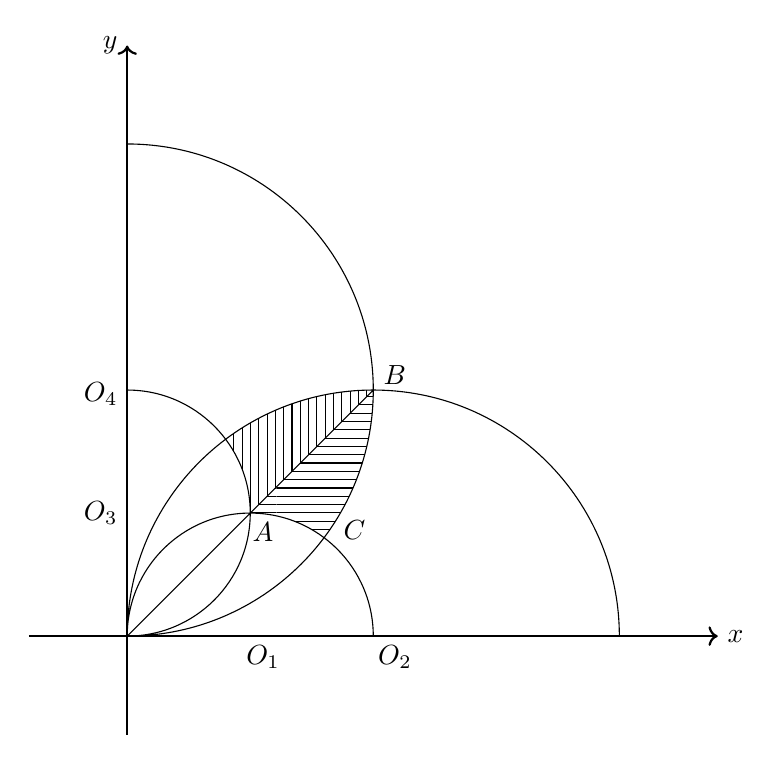
\begin{tikzpicture}[scale=25]
			\begin{scope}
				\clip (0,0) arc (-90:0:1/8) arc (90:180:1/8);
				\fill[pattern=horizontal lines]
				(0,0) arc (-90:0:1/8) --(1/16,1/16) arc (90:0:1/16);
				\fill[pattern=vertical lines]
				(0,0) arc (180:90:1/8) --(1/16,1/16) arc (0:90:1/16);
			\end{scope}
			\draw [->,thick](-0.05,0)--(0.3,0);\draw [->,thick](0,-0.05)--(0,0.3);
			\node[right]at(0.3,0){$x$};\node[left]at(0,0.3){$y$};
			\draw (0,0) arc (-90:90:1/8) (0,0) arc (-90:90:1/16)
			(0,0) arc (180:0:1/8) (0,0) arc (180:0:1/16) (0,0)--(1/8,1/8);
			\node [below]at(0.069,0.0627){$A$};
			\node [above]at(0.136,0.123){$B$};
			\node [right]at(0.105,0.0541){$C$};
			\node [below]at(0.069,0){$O_{1}$};
			\node [below]at(0.136,0){$O_{2}$};
			\node [left]at(0,0.0627){$O_{3}$};
			\node [left]at(0,0.123){$O_{4}$};
		\end{tikzpicture}
		\caption{二重积分区域示意图}
	\end{figure}

	$$I=2\iint_{D_{ACB}}\frac{1}{xy}dxdy=2\int_{\arctan \frac{1}{2}}^{\frac{\pi}{4}}d\theta\int_{\frac{\cos \theta}{4}}^{\frac{\sin\theta}{2}}\frac{1}{r\sin\theta\cos\theta}dr$$
	$$I=2\int_{\arctan \frac{1}{2}}^{\frac{\pi}{4}}\frac{\ln2\tan \theta}{\sin\theta\cos\theta}d\theta=2\int_{ \frac{1}{2}}^{1}\frac{\ln2t}{t}dt=\ln^2 2$$
\end{solution}
\myspace{1}

2. $\text{当}n\text{充分大时},a-\dfrac{1}{n}<a_{n}<a+\dfrac{1}{n}\text{是数列}a_{n}\text{收敛于}a\text{的什么条件 ?}$
\begin{itemize}
	\item A. $\text{充分必要条件}$
	\item B. $\text{必要条件但非充分条件}$
	\item \hl{C}. $\text{充分条件但非必要条件}$
	\item D. $\text{既非充分也非必要条件}$
\end{itemize}
\myspace{1}
\begin{solution}
	
	(i).充分性: 
	
	$a-\dfrac{1}{n}<a_{n}<a+\dfrac{1}{n},\text{由夹逼定理得到: }$
	$$\lim\limits_{n\rightarrow +\infty}(a-\frac{1}{n})<\lim\limits_{n\rightarrow +\infty}a_{n}<\lim\limits_{n\rightarrow +\infty}(a+\frac{1}{n})$$
	
	我们有: $\lim\limits_{n\rightarrow +\infty}(a-\frac{1}{n})=\lim\limits_{n\rightarrow +\infty}(a+\frac{1}{n})=a$
	因此: 
	$$\lim\limits_{n\rightarrow +\infty}a_{n}=a\Rightarrow\text{充分性成立}$$
	
	(ii).必要性
	
	$\lim\limits_{n\rightarrow +\infty}a_{n}=a\Rightarrow \forall \varepsilon>0,\ \exists N_{0}>0,\text{当}n>N_{0},|a_{n}-a|<\varepsilon$
	
	我们得到: 
	$$n>N_{0},a-\varepsilon<a_{n}<a+\varepsilon,\text{当}\frac{1}{N_{0}+1}<\varepsilon,\text{我们不能得到}a-\frac{1}{n}<a_{n}<a+\frac{1}{n},\text{必要性不成立}$$
	
	答案:$C$
\end{solution}
\myspace{1}

\hl{\textbf{\textit{May 18}}}

1. $\iint\limits_{D}|x^2+y^2-\sqrt{2}(x+y)|dxdy,\ D=\{(x,y)|x^2+y^2\leq 4\}$
\myspace{1}
\begin{solution}
	
	原二重积分等价于: 
	$$I=I_{1}+2I_{2}=\iint\limits_{D}[x^2+y^2-\sqrt{2}(x+y)]dxdy+2\iint\limits_{D_{1}}[\sqrt{2}(x+y)-(x^2+y^2)]dxdy$$
	$$I_{1}=\int_{0}^{2\pi}d\theta\int_{0}^{2}r(r^2-\sqrt{2}r(\sin \theta+\cos \theta))dr=\int_{0}^{2\pi}(4-\frac{8\sqrt{2}}{3}(\sin\theta+\cos\theta))d\theta=8\pi$$
	$$I_{2}=\iint\limits_{D_{1}}[\sqrt{2}(x+y)-(x^2+y^2)]dxdy,D_{1}: (x-\frac{\sqrt{2}}{2})^2+(y-\frac{\sqrt{2}}{2})^2\leq 1$$
	
	做变量替换: $\left\lbrace 
	\begin{array}{l}
		x-\frac{\sqrt{2}}{2}=R\cos \alpha\\
		y-\frac{\sqrt{2}}{2}=R\sin \alpha
	\end{array}
	\right. \Rightarrow dxdy=\left| \dfrac{\partial (x,y)}{\partial (R,\alpha)}\right| dRd\alpha=RdRd\alpha$
	
	$$I_{2}=\int_{0}^{2\pi}d\alpha\int_{0}^{1} (1-R^2)RdR=\frac{\pi}{2}$$
	$$I=I_{1}+2I_{2}=9\pi$$
\end{solution}
\myspace{1}

2. 设$f(x)$可积,则下列结论正确的是: 
\begin{itemize}
	\item A.$\text{如果}\lim\limits_{n\rightarrow +\infty}x_{n}=0,\text{且}\lim\limits_{n\rightarrow +\infty}f(x_{n})=A,\text{则}\lim\limits_{x\rightarrow 0}f(x)=A$
	\item B.$\text{如果}\lim\limits_{n\rightarrow +\infty}x_{n}=0,\text{且}\lim\limits_{x\rightarrow 0}f(x)=A,\text{则}\lim\limits_{n\rightarrow +\infty}f(x_{n})=A$
	\item C.$\text{如果}\lim\limits_{n\rightarrow +\infty}f(n)=A,\text{则}\lim\limits_{x\rightarrow +\infty}f(x)=A$
	\item \hl{D}.$\text{如果}\lim\limits_{n\rightarrow +\infty}\int_{0}^{n}\dfrac{|f(t)|}{1+t^2}dt=A,\text{则}\lim\limits_{x\rightarrow +\infty}\int_{0}^{x}\dfrac{|f(t)|}{1+t^2}dt=A$
\end{itemize}
\myspace{1}
\begin{solution}
	
	针对于此题,我们需要区分几个概念: 
	
	$$\lim\limits_{x\rightarrow x_{0}}f(x)=A, \text{只要求在}x\text{邻域内有定义,不要求}x\text{处有定义}$$
	$$\lim\limits_{n\rightarrow+\infty}f(n)=A,f(x)\text{单调},\Rightarrow \lim\limits_{x\rightarrow+\infty}f(x)=A$$
	
	对于$A$,我们只能得到在$x=0$的邻域内的一组特殊的离散点满足极限的定义,其余点未知,我们举一个反例,$x_{n}=\dfrac{1}{n\pi},f(x)=\sin\dfrac{1}{x}$
	
	对于$B$,我们举出一个反例$f(x)=\left\lbrace 
	\begin{array}{l}
		\dfrac{\sin x}{x},x\neq 0\\
		2
	\end{array}
	\right. $,$x_{n}=\left\lbrace 
	\begin{array}{l}
		\dfrac{1}{n},n\text{为奇数}\\
		0,n\text{为偶数}
	\end{array}
	\right. $
	
	对于$C$,不清楚$f(x)$单调性,举一个反例,$f(x)=\sin \pi x$
	
	对于$D$,利用积分的几何意义知道$g(x)=\int_{0}^{x}\dfrac{|f(t)|}{1+t^2}dt$单调递增
	
	答案:$D$.
\end{solution}
\myspace{1}

\hl{\textbf{\textit{May 19}}}

1. 设$f(u,v)$具有二阶连续偏导数,且满足$\dfrac{\partial^2 f}{\partial u^2}+\dfrac{\partial^2 f}{\partial v^2}=1$,又$g(x,y)=f(xy,\frac{1}{2}(x^2-y^2))$,求$\dfrac{\partial^2 g}{\partial x^2}+\dfrac{\partial^2 g}{\partial y^2}$
\myspace{1}
\begin{solution}
	
	我们令$\left\lbrace 
	\begin{array}{l}
		u=xy\\
		v=\dfrac{1}{2}(x^2-y^2)
	\end{array}
	\right. $
	
	我们有: 
	
	$$\left\lbrace 
	\begin{array}{l}
		\dfrac{\partial g}{\partial x}=\dfrac{\partial f}{\partial u}\dfrac{\partial u}{\partial x}+\dfrac{\partial f}{\partial v}\dfrac{\partial v}{\partial x}=y\dfrac{\partial f}{\partial u}+x\dfrac{\partial f}{\partial v}\\
		
		\\
		\dfrac{\partial g}{\partial y}=\dfrac{\partial f}{\partial u}\dfrac{\partial u}{\partial y}+\dfrac{\partial f}{\partial v}\dfrac{\partial v}{\partial y}=x\dfrac{\partial f}{\partial u}-y\dfrac{\partial f}{\partial v}
	\end{array}
	\right. $$
	$$\left\lbrace 
	\begin{array}{l}
		\dfrac{\partial^2 g}{\partial x^2}=y(y\dfrac{\partial^2 f}{\partial u^2}+x\dfrac{\partial^2 f}{\partial u\partial v})+\dfrac{\partial f}{\partial v}+x(y\dfrac{\partial^2 f}{\partial u\partial v}+x\dfrac{\partial^2 f}{\partial v^2})\\
		
		\\
		\dfrac{\partial^2 g}{\partial y^2}=x(x\dfrac{\partial^2 f}{\partial u^2}-y\dfrac{\partial^2 f}{\partial u\partial v})-\dfrac{\partial f}{\partial v}-y(x\dfrac{\partial^2 f}{\partial u\partial v}-y\dfrac{\partial^2 f}{\partial v^2})
	\end{array}
	\right. $$
	
	我们得到: 
	$$\dfrac{\partial^2 g}{\partial x^2}+\dfrac{\partial^2 g}{\partial y^2}=(x^2+y^2)\dfrac{\partial^2 f}{\partial u^2}+\dfrac{\partial^2 f}{\partial v^2}=x^2+y^2$$
\end{solution}
\myspace{1}

2. $\int_{-\pi}^{\pi}\dfrac{x\sin x\arctan e^{x}}{1+\cos ^2 x}dx$
\myspace{1}
\begin{solution}
	
	区间再现
	
	$$I=\int_{-\pi}^{\pi}\dfrac{x\sin x(\dfrac{\pi}{2}-\arctan e^{x})}{1+\cos ^2 x}dx$$
	$$2I=\dfrac{\pi}{2}\int_{-\pi}^{\pi}\dfrac{x\sin x}{1+\cos ^2 x}dx=\pi\int_{0}^{\pi}\dfrac{x\sin x}{1+\cos ^2 x}dx$$
	
	令$J=\int_{0}^{\pi}\dfrac{x\sin x}{1+\cos ^2 x}dx$
	
	$$J=\int_{0}^{\pi}\dfrac{(\pi-x)\sin x}{1+\cos ^2 x}dx\Rightarrow 2J=\pi\int_{0}^{\pi}\dfrac{\sin x}{1+\cos ^2 x}dx=\dfrac{\pi^2}{2}$$
	
	$$J=\dfrac{\pi^2}{4},I=\dfrac{\pi}{2}J=\dfrac{\pi^3}{8}$$
\end{solution}
\myspace{1}

\hl{\textbf{\textit{May 20}}}

1. 求$\iint\limits_{D}\dfrac{1}{3x^2+y^2}dxdy,D\text{是由}x^2+y^2-xy=1,\ x^2+y^2-xy=2\text{和直线}y=\sqrt{3}x,\ y=0\text{围成}$
\myspace{1}
\begin{solution}
	
	原二重积分等价于: 
	$$I=\int_{0}^{\frac{\pi}{3}}d\theta\int_{r_{1}}^{r_{2}}\dfrac{r}{3r^2\cos ^2\theta+r^2\sin^2\theta}dr,\text{其中}\left\lbrace 
	\begin{array}{l}
		r_{1}=\sqrt{\dfrac{1}{1-\sin \theta\cos\theta}}\\
		r_{2}=\sqrt{\dfrac{2}{1-\sin \theta\cos\theta}}
	\end{array}
	\right. $$
	
	$$I=\frac{\ln 2}{2}\int_{0}^{\frac{\pi}{3}}\dfrac{1}{\sin^2\theta+3\cos^2\theta}d\theta=\frac{\ln 2}{2}\int_{0}^{\frac{\pi}{3}}\dfrac{1}{3+\tan^2\theta}d\tan \theta$$
	$$I=\frac{\ln 2}{2\sqrt{3}}\arctan(\frac{\tan\theta}{\sqrt{3}})|_{0}^{\sqrt{3}}=\frac{\pi \ln 2}{8\sqrt{3}}$$
\end{solution}
\myspace{1}

2. $f(x)\text{在}[0,1]\text{上连续},\forall x,y\in \mathbb{R} ,|f(x)-f(y)|\leq M|x-y|,\text{求证: }\left| \int_{0}^{1}f(x)dx-\dfrac{1}{n}\sum\limits_{k=1}^{n}f(\dfrac{k}{n})\right|\leq \dfrac{M}{2n} $
\myspace{1}
\begin{solution}
	\begin{lemma}[积分和求和]
		
		$$\int_{0}^{1}f(x)dx=\sum\limits_{k=1}^{n}\int_{\frac{k-1}{n}}^{\frac{k}{n}}f(x)dx$$
	\end{lemma}
	我们利用上面的式子,对不等式的左边进行处理: 
	$$\text{左边: }\left| \sum\limits_{k=1}^{n}\int_{\frac{k-1}{n}}^{\frac{k}{n}}f(x)dx-\sum\limits_{k=1}^{n}\int_{\frac{k-1}{n}}^{\frac{k}{n}}f(\frac{k}{n})dx\right|=\left|\sum\limits_{k=1}^{n}\int_{\frac{k-1}{n}}^{\frac{k}{n}}[f(x)-f(\frac{k}{n})]dx\right|$$
	
	由绝对值不等式得到: 
	$$\text{左边}\leq \sum\limits_{k=1}^{n}\int_{\frac{k-1}{n}}^{\frac{k}{n}}\left|  [f(x)-f(\frac{k}{n})]\right|dx\leq  \sum\limits_{k=1}^{n}\int_{\frac{k-1}{n}}^{\frac{k}{n}}M(\frac{k}{n}-x)dx$$
	$$\text{左边}\leq M\sum\limits_{k=1}^{n}\frac{1}{2n^2}=\dfrac{M}{2n}=\text{右边} $$
\end{solution}
\myspace{1}

\hl{\textbf{\textit{May 21}}}

1. 已知数列$\{x_{n}\}$,且$\lim\limits_{n\rightarrow +\infty}\dfrac{x_{n}}{x_{n+1}}=\int_{0}^{1}e^{-x^2}dx$,则: 
\begin{itemize}
	\item A.$\lim\limits_{n\rightarrow +\infty}=0$
	\item \hl{B}.$\lim\limits_{n\rightarrow +\infty}=\infty$
	\item C.$\lim\limits_{n\rightarrow +\infty}=a\ (a\neq 0)$
	\item D.$\lim\limits_{n\rightarrow +\infty}\text{不存在但不是}\infty$
\end{itemize}
\myspace{1}
\begin{solution}
	
	首先我们可以得到: 
	$$\int_{0}^{1}e^{-x^2}dx=a,\ a\in(0,1)$$
	
	我们由$\lim\limits_{n\rightarrow +\infty}\frac{x_{n}}{x_{n+1}}=a\Rightarrow |x_{n}|=a|x_{n+1}|<|x_{n+1}|\Rightarrow x_{n}\text{单调递增}$
	
	我们假设$x_{n}$有上界
	$$\lim\limits_{n\rightarrow +\infty}x_{n}=\lim\limits_{n\rightarrow +\infty}x_{n+1}\Rightarrow \lim\limits_{n\rightarrow +\infty}\frac{x_{n}}{x_{n+1}}=1\neq a\text{矛盾!!!}$$
	
	答案:$B$
\end{solution}
\myspace{1}

2. 设$f(x,y)\text{二阶偏导数连续},f(1,y)=f(x,1)=0,\iint\limits_{D}f(x,y)dxdy=a$,其中$D\in [0,1]\times [0,1]$,计算$\iint\limits_{D}xyf''_{xy}(x,y)d\sigma$
\myspace{1}
\begin{solution}
	
	原二重积分可以化为: 
	\begin{eqnarray*}
		\int_{0}^{1}xdx\int_{0}^{1}ydf'_{x}(x,y)&=&\int_{0}^{1}x\left[yf'_{x}(x,y)|_{y=0}^{y=1}-\int_{0}^{1}f'_{x}(x,y)dy\right]dx\\
		&=&-\int_{0}^{1}xdx\int_{0}^{1}f'_{x}(x,y)dy\\
		&=&-\int_{0}^{1}dy\int_{0}^{1}xdf(x,y)\\
		&=&-\int_{0}^{1}\left[xf(x,y)|_{x=0}^{x=1}-\int_{0}^{1}f(x,y)dx\right]dy\\
		&=&\int_{0}^{1}dx\int_{0}^{1}f(x,y)dy=a
	\end{eqnarray*}
	
	$$\iint\limits_{D}xyf''_{xy}(x,y)d\sigma=\int_{0}^{1}dx\int_{0}^{1}f(x,y)dy=a$$
\end{solution}
\myspace{1}

\section{Week \Rmnum{4}}
\hl{\textbf{\textit{May 22}}}

1. 设$a_{n}=\int_{0}^{1}x^{n}\sqrt{1-x^2}dx\ (n=0,1,2,\cdots)$

(1).$\text{证明: 数列}\{a_{n}\}\text{单调减少,且}a_{n}=\dfrac{n-1}{n+2}a_{n-2},\ (n=2,3,\cdots)$

(2). $\text{求}\lim\limits_{n\rightarrow \infty}\dfrac{a_{n}}{a_{n-1}}$
\myspace{1}
\begin{solution}
	
	(1).
	我们令$x=\sin t,\ t\in[0,\frac{\pi}{2}],\ dx=\cos tdt$,我们有: 
	$$a_{n}=\int_{0}^{\frac{\pi}{2}}\sin^{n}t\cos^{2} tdt=\int_{0}^{\frac{\pi}{2}}\sin^{n}tdt-\int_{0}^{\frac{\pi}{2}}\sin^{n+2}tdt$$
	$$a_{0}=\frac{\pi}{4},\ a_{1}=\frac{1}{3}$$
	
	根据华里士公式,我们有: 
	$$\int_{0}^{\frac{\pi}{2}}\sin^{n}xdx=\left\lbrace 
	\begin{array}{l}
		\dfrac{n-1}{n}\cdot\dfrac{n-3}{n-2}\cdots\dfrac{2}{3}\cdot 1,n\text{为大于1的奇数}\\
		\dfrac{n-1}{n}\cdot\dfrac{n-3}{n-2}\cdots\dfrac{1}{2}\cdot\dfrac{\pi}{2},n\text{为正偶数}
	\end{array}
	\right. $$
	$$a_{n}-a_{n-1}=\int_{0}^{\frac{\pi}{2}}\sin^{n}tdt-\int_{0}^{\frac{\pi}{2}}\sin^{n+2}tdt-\int_{0}^{\frac{\pi}{2}}\sin^{n-1}tdt+\int_{0}^{\frac{\pi}{2}}\sin^{n+1}tdt$$
	$$a_{n}-a_{n-1}=\int_{0}^{\frac{\pi}{2}}-(1-\sin t)^2\sin^{n-1}tdt<0\Rightarrow a_{n}<a_{n-1}\Rightarrow \{a_{n}\}\text{单调递减}$$
	
	(i). 当$n$为奇数时,我们有: 
	$$\left\lbrace 
	\begin{array}{l}
		a_{n}=(1-\dfrac{n+1}{n+2})\dfrac{n-1}{n}\cdot\dfrac{n-3}{n-2}\cdots\dfrac{2}{3}\cdot 1\\
		a_{n-2}=(1-\dfrac{n-1}{n})\dfrac{n-3}{n-2}\cdots\dfrac{2}{3}\cdot 1
	\end{array}
	\right. $$
	$$\left\lbrace 
	\begin{array}{l}
		a_{n}=\dfrac{n-1}{n+2}\cdot\dfrac{1}{n}\cdot\dfrac{n-3}{n-2}\cdots\dfrac{2}{3}\cdot 1\\
		a_{n-2}=\dfrac{1}{n}\cdot\dfrac{n-3}{n-2}\cdots\dfrac{2}{3}\cdot 1
	\end{array}
	\right. 
	$$
	$$a_{n}=\dfrac{n-1}{n+2}a_{n-2}$$
	
	(i). 当$n$为偶数数时,我们有: 
	$$\left\lbrace 
	\begin{array}{l}
		a_{n}=(1-\dfrac{n+1}{n+2})\dfrac{n-1}{n}\cdot\dfrac{n-3}{n-2}\cdots\dfrac{1}{2}\cdot\dfrac{\pi}{2}\\
		a_{n-2}=(1-\dfrac{n-1}{n})\dfrac{n-3}{n-2}\cdots\dfrac{1}{2}\cdot\dfrac{\pi}{2}
	\end{array}
	\right. $$
	$$\left\lbrace 
	\begin{array}{l}
		a_{n}=\dfrac{n-1}{n+2}\cdot\dfrac{1}{n}\cdot\dfrac{n-3}{n-2}\cdots\dfrac{1}{2}\cdot\dfrac{\pi}{2}\\
		a_{n-2}=\dfrac{1}{n}\cdot\dfrac{n-3}{n-2}\cdots\dfrac{1}{2}\cdot\dfrac{\pi}{2}
	\end{array}
	\right. 
	$$
	$$a_{n}=\frac{n-1}{n+2}a_{n-2}$$
	
	综上所述,$\text{数列}\{a_{n}\}\text{单调减少,且}a_{n}=\dfrac{n-1}{n+2}a_{n-2},\ (n=2,3,\cdots)$
	
	(2). 我们不妨设$b_{n}=\dfrac{a_{n}}{a_{n-1}},\ (n=1,2,\cdots)$
	
	$b_{1}=\dfrac{4}{3\pi}$,当$n\geq 2$是,我们有: 
	
	$$b_{n}b_{n-1}=\dfrac{a_{n}}{a_{n-1}}\cdot\dfrac{a_{n-1}}{a_{n-2}}=\dfrac{n-1}{n+2}$$
	
	不妨设$\lim\limits_{n\rightarrow \infty}b_{n}=A$
	$$ A^2=\lim\limits_{n\rightarrow \infty}\dfrac{n-1}{n+2}=1\Rightarrow A=1(A>0)$$
	
	我们来严格证明$\lim\limits_{n\rightarrow \infty}\dfrac{a_{n}}{a_{n-1}}=1$
	
	原命题转换为: 
	
	$$\forall \varepsilon>0,\ \exists N>0,\text{当}n>N\text{时},|\dfrac{a_{n}}{a_{n-1}}-1|<\epsilon$$
	$$\int_{0}^{1}(1-x)x^{n-1}\sqrt{1-x^2}dx<\varepsilon \int_{0}^{1}x^{n-1}\sqrt{1-x^2}dx\Rightarrow \int_{0}^{1}(1-x-\varepsilon)x^{n-1}\sqrt{1-x^2}dx<0$$
	$$\int_{0}^{1-\varepsilon}(1-x-\varepsilon)x^{n-1}\sqrt{1-x^2}dx<\int_{1-\varepsilon}^{1}(x+\varepsilon-1)x^{n-1}\sqrt{1-x^2}dx$$
	
	$$\text{左式}<(1-\varepsilon)^{n-1}\int_{0}^{1}x^{n-1}\sqrt{1-x^2}dx=P(1-\varepsilon)^{n-1}$$
	$$\text{右式}>\int_{1-\frac{\varepsilon}{2}}^{1}(x+\varepsilon-1)x^{n-1}\sqrt{1-x^2}dx>(1-\frac{\varepsilon}{2})^{n-1}\int_{1-\frac{\varepsilon}{2}}^{1}(x+\varepsilon-1)\sqrt{1-x^2}dx>Q(1-\frac{\varepsilon}{2})^{n-1}$$
	
	其中$P,Q$均为与$n$无关的正数,我们只需找到$N$,使得$Q(1-\dfrac{\varepsilon}{2})^{n-1}>P(1-\varepsilon)^{n-1}$
	$$n>[1+\dfrac{\ln P-\ln Q}{\ln(1-\frac{\varepsilon}{2})-\ln(1-\varepsilon)}]$$
	
	综上,$\forall \varepsilon>0,\ \exists N=[1+\dfrac{\ln P-\ln Q}{\ln(1-\frac{\varepsilon}{2})-\ln(1-\varepsilon)}]+1>0,\text{当}n>N\text{时},|\dfrac{a_{n}}{a_{n-1}}-1|<\epsilon$
\end{solution}
\begin{anymark}[注]
	(1). 我们可以得到: 
	$$a_{n+1}-a_{n}=\int_{0}^{1}x^{n+1}\sqrt{1-x^2}dx-\int_{0}^{1}x^{n}\sqrt{1-x^2}dx=\int_{0}^{1}(x-1)x^{n}\sqrt{1-x^2}dx<0$$
	
	我们可以得到数列$\{a_{n}\}$单调递减.
	
	我们还有: 
	\begin{eqnarray*}
		a_{n}&=&\int_{0}^{1}x^{n}\sqrt{1-x^2}dx\\
		&=&-\dfrac{1}{3}\int_{0}^{1}x^{n-1}d(1-x^2)^{\frac{3}{2}}\\
		&=&\dfrac{n-1}{3}\int_{0}^{1}x^{n-2}\sqrt{1-x^2}(1-x^2)dx\\
		&=&\dfrac{n-1}{3}a_{n-2}-\dfrac{n-1}{3}a_{n}\\
		a_{n}&=&\dfrac{n-1}{n+2}a_{n-2}
	\end{eqnarray*}
	
	(2). 我们由(1)知道,$\{a_{n}\}$单调递减且$a_{n}>0$,我们得到: 
	$$\left\lbrace
	\begin{array}{l}
		a_{n}<a_{n-1}\\a_{n-1}<a_{n-2}
	\end{array}
	\right. \Rightarrow \left\lbrace
	\begin{array}{l}
		\dfrac{a_{n}}{a_{n-1}}<1\\\dfrac{a_{n}}{a_{n-2}}<\dfrac{a_{n}}{a_{n-1}}
	\end{array}
	\right. $$
	
	我们由夹逼定理可以得到: 
	$$\left\lbrace
	\begin{array}{l}
		\lim\limits_{n\rightarrow +\infty}\dfrac{a_{n}}{a_{n-2}}=1\\
		\lim\limits_{n\rightarrow +\infty}1=1
	\end{array}
	\right. \Rightarrow \lim\limits_{n\rightarrow +\infty}\dfrac{a_{n}}{a_{n-1}}=1$$
	
	综上所述,我们得到: $\lim\limits_{n\rightarrow +\infty}\dfrac{a_{n}}{a_{n-1}}=1$
\end{anymark}
\myspace{1}

2. $xy'-(2x^2+1)y=x^2(x\geq 1)$,且$y(1)=a$,讨论$\lim\limits_{x\rightarrow +\infty}y(x)$
\myspace{1}
\begin{solution}
	
	我们得到微分方程: 
	$$y'-(2x+\frac{1}{x})y=x\Rightarrow (e^{\int (-2x-\frac{1}{x})dx}y)'=xe^{\int (2x+\frac{1}{x})dx}$$
	
	$$y=xe^{x^2}(\int_{1}^{x}e^{-t^2}dt+C)$$
	
	我们由: $y(1)=a\Rightarrow C=\dfrac{a}{e}$
	
	原问题转化为: 
	$$\lim\limits_{x\rightarrow +\infty}xe^{x^2}(\int_{1}^{x}e^{-t^2}dt+\frac{a}{e})$$
	
	我们有: $$\int_{0}^{+\infty}e^{-x^2}dx=\frac{\sqrt{\pi}}{2}$$
	
	原极限可以写作: 
	$$\lim\limits_{x\rightarrow +\infty}xe^{x^2}(\frac{\sqrt{\pi}}{2}-\int_{0}^{1}e^{-t^2}dt+\frac{a}{e})$$
	
	(i).当$a=e(\int_{0}^{1}e^{-t^2}dt-\dfrac{\sqrt{\pi}}{2})$
	
	洛必达法则: $$\lim\limits_{x\rightarrow +\infty}xe^{x^2}(\frac{\sqrt{\pi}}{2}-\int_{0}^{1}e^{-t^2}dt+\frac{a}{e})=\lim\limits_{x\rightarrow +\infty}\frac{x^2}{-2x^2-1}=-\frac{1}{2}$$
	
	(ii).当$a\neq e(\int_{0}^{1}e^{-t^2}dt-\dfrac{\sqrt{\pi}}{2})$,极限不存在.
\end{solution}
\myspace{1}

\hl{\textbf{\textit{May 23}}}

1. 已知当$n$充分大时,$|a_{n}|\leq |b_{n}|\leq |c_{n}|$,且$\lim\limits_{x\rightarrow \infty}a_{n}=\lim\limits_{x\rightarrow \infty}|c_{n}|$,则: 
\begin{itemize}
	\item A. $\lim\limits_{x\rightarrow \infty}(|a_{n}|-b_{n})$
	\item B. $\lim\limits_{x\rightarrow \infty}(|b_{n}|-c_{n})$
	\item C. $\lim\limits_{x\rightarrow \infty}(|b_{n}|-c_{n})$
	\item \hl{D}. $\lim\limits_{x\rightarrow \infty}(|b_{n}|-a_{n})$
\end{itemize}
\myspace{1}
\begin{solution}
	
	我们有: $\lim\limits_{x\rightarrow \infty}x_{n}=A\Rightarrow \lim\limits_{x\rightarrow \infty}|x_{n}|=A$
	
	我们假设: $\lim\limits_{x\rightarrow \infty}a_{n}=\lim\limits_{x\rightarrow \infty}|c_{n}|=A$
	
	我们得到: $\lim\limits_{x\rightarrow \infty}|a_{n}|=A$
	
	根据夹逼定理: $\lim\limits_{x\rightarrow \infty}|b_{n}|=A$
	
	我们已知的极限有$\lim\limits_{x\rightarrow \infty}a_{n},\lim\limits_{x\rightarrow \infty}|a_{n}|,\lim\limits_{x\rightarrow \infty}|b_{n}|,\lim\limits_{x\rightarrow \infty}|c_{n}|$
	
	答案:$D$.
\end{solution}
\myspace{1}

2. $\lim\limits_{n\rightarrow+\infty}\sin^{2}(\pi\sqrt{n^2+3n})$
\myspace{1}
\begin{solution}
	
	原极限等价于: 
	\begin{eqnarray*}
		\lim\limits_{n\rightarrow+\infty}\sin^{2}(\pi\sqrt{n^2+3n}-\pi n)&=&\lim\limits_{n\rightarrow+\infty}\sin^{2}(\dfrac{3n\pi }{\sqrt{n^2+3n}+n})\\
		&=&\sin^2(\frac{3\pi}{2})=1
	\end{eqnarray*}	
\end{solution}
\myspace{1}

\hl{\textbf{\textit{May 24}}}

1. $\lim\limits_{n\rightarrow +\infty}\dfrac{1}{\sqrt[n]{n!}}\left[\dfrac{1}{n+\ln 1}+\dfrac{2}{n+\ln 2}+\cdots+\dfrac{n}{n+\ln n} \right]$
\myspace{1}
\begin{lemma}[斯特林公式]\label{lem: 斯特林公式}
	$$n!\approx \sqrt{2\pi n}(\dfrac{n}{e})^n$$
\end{lemma}
\begin{anymark}[注]
	\begin{eqnarray*}
		\lim\limits_{n\to +\infty}\dfrac{n}{\sqrt[n]{n!}}
		& = &\lim\limits_{n\to +\infty}e^{-\frac{1}{n}(\ln\frac{1}{n}+\ln\frac{2}{n}+\cdots+\ln\frac{n}{n})}\\
		& = &e^{-\int_{0}^{1}\ln x dx}\\
		& = &e
	\end{eqnarray*}
\end{anymark}
\begin{solution}
	
	我们不妨设$b_{n}=\dfrac{1}{\sqrt[n]{n!}}\left[\dfrac{1}{n+\ln 1}+\dfrac{2}{n+\ln 2}+\cdots+\dfrac{n}{n+\ln n} \right]$
	$$a_{n}=\dfrac{1}{\sqrt[n]{n!}}[\frac{1}{n}+\frac{2}{n}+\cdots+\frac{n}{n}],\ c_{n}=\dfrac{1}{\sqrt[n]{n!}}[\frac{1}{n+\ln n}+\frac{2}{n+\ln n}+\cdots+\frac{n}{n+\ln n}]$$
	
	我们得到: 
	$$c_{n}<b_{n}<a_{n}\Rightarrow \dfrac{n+1}{2(n+\ln n)}\dfrac{n}{\sqrt[n]{n!}}<b_{n}<\dfrac{n+1}{2n}\dfrac{n}{\sqrt[n]{n!}}$$
	
	我们有: $\lim\limits_{n\rightarrow +\infty}\dfrac{n+1}{2(n+\ln n)}=\lim\limits_{n\rightarrow +\infty}\dfrac{n+1}{2n}=\dfrac{1}{2}$
	
	对于$\lim\limits_{n\rightarrow +\infty}\dfrac{n}{\sqrt[n]{n!}}$
	
	我们可以知道: $\lim\limits_{n\rightarrow +\infty}\dfrac{n}{\sqrt[n]{n!}}=e$
	
	我们得到: $\lim\limits_{n\rightarrow +\infty}a_{n}=\lim\limits_{n\rightarrow +\infty}b_{n}=\dfrac{e}{2}$
	
	由夹逼定理,我们得到: $\lim\limits_{n\rightarrow +\infty}b_{n}=\dfrac{e}{2}$
\end{solution}
\myspace{1}

2. $f(x)>0,f(x)f''(x)\geq [f'(x)]^2,f(0)=1$,证明: $f(x)\geq e^{f'(0)x}$
\myspace{1}
\begin{solution}
	
	这个题还有第一问: $f(x_{1})f(x_{2})\geq f^2(\dfrac{x_{1}+x_{2}}{2})$
	
	我们由: $$f(x)f''(x)\geq [f'(x)]^2\Rightarrow \text{可以构造出函数}\frac{f'(x)}{f(x)}\text{单调递增}$$
	
	我们将$f(x_{1})f(x_{2})\geq f^2(\dfrac{x_{1}+x_{2}}{2})$取对数得到: 
	$$\ln f(x_{1})+\ln f(x_{2})\geq 2\ln f(\frac{x_{1}+x_{2}}{2})$$
	
	我们构造函数$g(x)=\ln f(x)$
	
	原命题转化为: $\dfrac{g(x_{1})+g(x_{2})}{2}\geq g(\frac{x_{1}+x_{2}}{2})$
	
	我们只需要证明: $g(x)\text{是凹函数},g''(x)\geq 0$
	
	我们有: $$g'(x)=\dfrac{f'(x)}{f(x)},\ g''(x)=\dfrac{f(x)f''(x)-[f'(x)]^2}{f^2(x)}\geq 0$$
	
	$g(x)\text{为凹函数}\Rightarrow \dfrac{g(x_{1})+g(x_{2})}{2}\geq g(\frac{x_{1}+x_{2}}{2})$
	
	我们证明了: $f(x_{1})f(x_{2})\geq f^2(\frac{x_{1}+x_{2}}{2})$
	
	$$g''(x)\geq 0\Rightarrow g'(x)\geq g'(0)=\dfrac{f'(0)}{f(0)}$$
	
	我们可以理解为: $g(x)\text{始终大于}g(0)\text{处的切线}$
	
	$$g(x)\geq g'(0)x+g(0)\Rightarrow \ln f(x)\geq f'(0)x\Rightarrow f(x)\geq e^{f'(0)x}$$
\end{solution}
\myspace{1}

\hl{\textbf{\textit{May 25}}}

1. 设$f'(x)$在$[a,b]$上连续,且$f(a)=f(b)=0$,证明: $|f(x)|\leq \frac{1}{2}\int_{a}^{b}|f'(x)|dx$
\myspace{1}
\begin{solution}
	
	我们可以得到: $$f(x)=f(x)-f(a)=\int_{a}^{x}f'(t)tdt,\ f(x)=-(f(b)-f(x))=-\int_{x}^{b}f'(t)tdt$$
	
	我们得到: 
	$$\left\lbrace 
	\begin{array}{l}
		|f(x)|=|\int_{a}^{x}f'(t)tdt|\leq\int_{a}^{x}|f'(t)|dt\\
		|f(x)|=|\int_{x}^{b}f'(t)tdt|\leq\int_{x}^{b}|f'(t)|dt
	\end{array}
	\right. \Rightarrow 2|f(x)|\leq\int_{a}^{b}|f'(x)|dx$$
	
	我们证明: $|f(x)|\leq \frac{1}{2}\int_{a}^{b}|f'(x)|dx$
\end{solution}
\myspace{1}

2. $\iint_{D}\ln|sin(x-y)|dxdy,\ D=\{(x,y)|0\leq x\leq y\leq 2\pi\}$
\myspace{1}
\begin{solution}
	
	利用二重积分换元公式: $\left\lbrace 
	\begin{array}{l}
		u=y-x\\
		v=x
	\end{array}
	\right.\Rightarrow dudv=dxdy,\ 0\leq u\leq \pi-v,0\leq v\leq \pi$
	
	我们得到原二重积分等价于: 
	$$I=\int_{0}^{\pi}du\int_{0}^{\pi-u}\ln(sin u)dudv=\int_{0}^{\pi}(\pi-u)\ln(\sin u)du$$
	
	利用区间再现公式: 
	$$2I=\pi\int_{0}^{\pi}\ln(\sin u)du\Rightarrow I=\pi\int_{0}^{\frac{\pi}{2}}\ln(\sin u)du$$
	
	$$I=-\frac{\ln 2\pi^2}{2}$$
	\begin{lemma}[区间再现例子]
		\begin{itemize}
			\item $\int_{0}^{\pi}\ln(\sin x)dx=\int_{0}^{\pi}\ln(\cos x)dx=-\dfrac{\ln 2\pi}{2}$
			\item $\int_{0}^{\frac{\pi}{2}}\ln(\tan x)dx=0$
		\end{itemize}
		\begin{anymark}[注]
			$$\int_{0}^{\frac{\pi}{2}}\ln(\sin x)dx=\int_{0}^{\frac{\pi}{2}}\ln(\cos x)dx$$
			
			我们有: 
			\begin{eqnarray*}
				2I&=&\int_{0}^{\frac{\pi}{2}}\ln(\sin x\cos x)dx\\
				&=&\int_{0}^{\frac{\pi}{2}}\ln(\sin 2x)dx-\int_{0}^{\frac{\pi}{2}}\ln 2dx\\
				&=&I-\frac{\ln 2\pi}{2}\\
				I&=&-\frac{\ln 2\pi}{2}
			\end{eqnarray*}
		\end{anymark}
		$$\int_{0}^{\pi}xf(\sin x)dx=\frac{\pi}{2}\int_{0}^{\pi}f(\sin x)dx$$
	\end{lemma}
\end{solution}
\myspace{1}

\hl{\textbf{\textit{May 26}}}

1. 设$x_{n}=(1+\dfrac{1}{n^2})(1+\dfrac{2}{n^2})\cdots(1+\dfrac{n}{n^2})$,求$\lim\limits_{n\rightarrow\infty}x_{n}$
\myspace{1}
\begin{solution}
	
	原极限等价于: 
	\begin{eqnarray*}
		I&=&\lim\limits_{n\rightarrow\infty}e^{\ln(1+\frac{1}{n^2})}e^{\ln(1+\frac{2}{n^2})}\cdots e^{\ln(1+\frac{n}{n^2})}\\
		&=&\lim\limits_{n\rightarrow\infty}e^{\frac{1}{n^2}}e^{\frac{2}{n^2}}\cdots e^{\frac{n}{n^2}}\\
		&=&\lim\limits_{n\rightarrow\infty}e^{\frac{n(n+1)}{2n^2}}\\
		&=&e^{\frac{1}{2}}
	\end{eqnarray*}
	\begin{lemma}[不等式放缩]
		\begin{itemize}
			\item $\text{琴生不等式: }\dfrac{2}{\pi}x\leq \sin x\leq x,x\in[0,\frac{\pi}{2}]$
			\item $\text{琴生不等式: }x\leq \tan x\leq \dfrac{4}{\pi}x,x\in[0,\frac{\pi}{4}]$
			\item $\text{泰勒不等式: }\dfrac{x}{1+x}\leq \ln(1+x)\leq x,\ x\in[0,+\infty)$
		\end{itemize}
	\end{lemma}
	我们利用不等式放缩: 
	$$\frac{k}{n^2+k}\leq \ln(1+\frac{k}{n^2})\leq \frac{k}{n^2}\Rightarrow \frac{k}{n^2+n}\leq \ln(1+\frac{k}{n^2})\leq \frac{k}{n^2}$$
	
	我们得到: 
	$$\sum\limits_{k=1}^{n}\frac{k}{n^2+n}\leq \sum\limits_{k=1}^{n}\ln(1+\frac{k}{n^2})\leq \sum\limits_{k=1}^{n}\frac{k}{n^2}$$
	
	$$\lim\limits_{n\rightarrow\infty}\sum\limits_{k=1}^{n}\frac{k}{n^2+n}=\lim\limits_{n\rightarrow\infty}\sum\limits_{k=1}^{n}\dfrac{k}{n^2}=\dfrac{1}{2}$$
	
	由夹逼定理,我们得到: $\sum\limits_{k=1}^{n}\ln(1+\dfrac{k}{n^2})=\dfrac{1}{2}\Rightarrow I=e^{\frac{1}{2}}$
\end{solution}
\myspace{1}

2. 若函数$\varphi(x)$具有二阶导数,且满足$\varphi(2)>\varphi(1)$,$\varphi(2)>\int_{2}^{3}\varphi(x)dx$,证明: 至少存在一点$\xi\in(1,3)$,$s.t.\varphi ''(x)<0$
\myspace{1}
\begin{solution}
	
	我们有积分中值定理得到: 
	$$\exists \eta\in(2,3),\ s.t. \int_{2}^{3}\varphi(x)dx=\varphi(\eta)$$
	
	我们由拉格朗日中值定理得到: 
	$$\left\lbrace 
	\begin{array}{l}
		\exists \xi_{1}\in(1,2),\ s.t. \dfrac{\varphi(2)-\varphi(1)}{2-1}=\varphi '(\xi_{1})>0\\
		\exists \xi_{2}\in(2,\eta),\ s.t. \dfrac{\varphi(\eta)-\varphi(2)}{\eta-2}=\varphi '(\xi_{2})<0
	\end{array}
	\right. $$
	
	我们在区间$(\xi_{1},\xi_{2})$内使用拉格朗日中值定理得到: 
	$$\exists \xi_{3}\in(\xi_{1},\xi_{2}),\ s.t. \dfrac{\varphi(\xi_{2})-\varphi(\xi_{1})}{\xi_{2}-\xi_{1}}=\varphi '(\xi_{3})<0$$
	
	综上所述,我们得到: $\exists \xi\in(1,3)$,$s.t.\varphi ''(x)<0$
\end{solution}
\myspace{1}

\hl{\textbf{\textit{May 27}}}

1. 设$x_{0}=0,x_{n}=\dfrac{1+2x_{n-1}}{1+x_{n-1}}$,证明数列$\{x_{n}\}$收敛,并求极限$\lim\limits_{n\rightarrow +\infty}x_{n}$
\myspace{1}
\begin{solution}
	
	我们有: $x_{1}=1,x_{2}=\dfrac{3}{2},x_{n}>0$
	
	我们使用数学归纳法来证明$x_{n}$单调递增: ($x_{n+1}>x_{n}$)
	
	(1).当$n=1$时,$x_{2}>x_{1}$成立
	
	(2).当$n\geq 1$时,假设$n=k$时,$x_{k+1}>x_{k}$,我们有: 
	$$x_{k+1}=\dfrac{1+2x_{k}}{1+x_{k}}>x_{k}\Rightarrow 1+2x_{k}-x_{k}>0$$
	
	当$n=k+1$时: 
	$$x_{k+2}=\dfrac{1+2\dfrac{1+2x_{k}}{1+x_{k}}}{1+\dfrac{1+2x_{k}}{1+x_{k}}}=\dfrac{3+5x_{k}}{2+3x_{k}}$$
	
	$$x_{k+2}-x_{k+1}=\dfrac{3+5x_{k}}{2+3x_{k}}-\dfrac{1+2x_{k}}{1+x_{k}}=\dfrac{1+2x_{k}-x_{k}^2}{(2+3x_{k})(1+x_{k})}>0$$
	
	我们证明: $x_{n}$单调递增,且$x_{n}-2x_{n}-1<0\Rightarrow |x_{n}|<3$
	
	$\{x_{n}\}$单调递增且有上界,我们得到$x_{n}$极限必定存在,我们不妨设: 
	
	$$\lim\limits_{n\rightarrow +\infty}x_{n}=A(A>0)\Rightarrow A=\frac{1+2A}{1+A}\Rightarrow A=\dfrac{1+\sqrt{5}}{2}$$
\end{solution}
\myspace{1}

2. $\lim\limits_{n\rightarrow +\infty}\int_{n}^{n+1}x^2\sin\dfrac{1}{x}dx$
\myspace{1}
\begin{solution}
	
	我们有: 
	$$\lim\limits_{x\rightarrow +\infty}x^2\sin\frac{1}{x}=\lim\limits_{x\rightarrow +\infty}x\dfrac{\sin\frac{1}{x}}{\frac{1}{x}}=+\infty$$
	
	我们有: $\lim\limits_{n\rightarrow +\infty}\int_{n}^{n+1}x^2\sin\dfrac{1}{x}dx=+\infty$
\end{solution}
\myspace{1}

\hl{\textbf{\textit{May 28}}}

1. 判断级数的敛散性: $\sum\limits_{n=1}^{+\infty}\dfrac{n+1}{\sqrt{n^5-n+2}}$和$\sum\limits_{n=1}^{+\infty}\dfrac{1}{\sqrt{n(n+1)}(\sqrt{n+1}+\sqrt{n})}$
\myspace{1}
\begin{solution}
	
	我们运用比较判别法的极限形式: 
	$$\lim\limits_{n\rightarrow +\infty}\dfrac{\dfrac{n+1}{\sqrt{n^5-n+2}}}{n^{-\frac{3}{2}}}=1$$
	
	原级数收敛.
	
	$$\lim\limits_{n\rightarrow +\infty}\dfrac{\frac{1}{\sqrt{n(n+1)}(\sqrt{n+1}+\sqrt{n})}}{2n^{-\frac{3}{2}}}=\frac{1}{2}$$
	
	原级数收敛.
\end{solution}
\myspace{1}

2. $f(x)$在$[0,1]$上连续,且$\int_{0}^{1}f(x)dx=A$,求$\int_{0}^{1}dx\int_{x}^{1}dy\int_{x}^{y}f(x)f(y)f(z)dz$
\myspace{1}
\begin{solution}
	
	我们不妨设: $F(x)=\int_{0}^{x}f(t)dt,\ F(0)=0,F(1)=A$,原积分等价于: 
	\begin{eqnarray*}
		I&=&\int_{0}^{1}dx\int_{x}^{1}f(x)f(y)[F(y)-F(x)]dy\\
		&=&\int_{0}^{1}f(x)dx\int_{x}^{1}f(y)F(y)dy-\int_{0}^{1}f(x)F(x)dx\int_{x}^{1}f(y)dy\\
		&=&\int_{0}^{1}f(x)[\dfrac{F^2(1)}{2}-\dfrac{F^2(x)}{2}]dx-\int_{0}^{1}f(x)F(x)[F(1)-F(x)]dx\\
		&=&\frac{A^3}{2}-\frac{A^3}{6}-\frac{A^3}{2}+\frac{A^3}{3}\\
		&=&\frac{A^3}{6}
	\end{eqnarray*}
\end{solution}
\myspace{1}

\hl{\textbf{\textit{May 29}}}

1. 判断级数$\sum\limits_{n=1}^{+\infty}(-1)^{n-1}\dfrac{2+(-1)^n}{n^2}$敛散性
\myspace{1}
\begin{solution}
	
	我们不妨设: $a_{n}=\sum\limits_{n=1}^{+\infty}(-1)^{n-1}\dfrac{2}{n^2}$,$b_{n}=\sum\limits_{n=1}^{+\infty}-\frac{1}{n^2}$
	
	我们根据莱布尼茨判别法得到: 
	$a_{n}$收敛,$b_{n}$收敛,原级数收敛.
\end{solution}
\myspace{1}

2. $\iint_{D}|\dfrac{x+y}{2}-x^2-y^2|dxdy,D=\{(x,y)|x^2+y^2\leq 1\}$
\myspace{1}
\begin{solution}
	
	原二重积分可化为: 
	$$I=\iint_{D}|\dfrac{1}{8}-(x-\dfrac{1}{4})^2-(y-\dfrac{1}{4})^2|dxdy,D:\{(x,y)|x^2+y^2\leq 1\}$$
	
	$$I=\iint_{D}(x^2+y^2-\dfrac{x+y}{2})dxdy-2\iint_{D'}(x^2+y^2-\dfrac{x+y}{2})dxdy$$
	
	其中: $$D=\{(x,y)|x^2+y^2\leq 1\},\ D'=\{(x,y)|(x-\frac{1}{4})^2+(y-\frac{1}{4})^2\leq \frac{1}{8}\}$$
	
	$$I=\int_{0}^{2\pi}d\theta\int_{0}^{1}[r^3-\frac{r^2}{2}(\sin\theta+\cos\theta)]dr-2\int_{-\frac{\pi}{4}}^{\frac{3\pi}{4}}d\theta\int_{0}^{\frac{\sin\theta+\cos\theta}{2}}[r^3-\frac{r^2}{2}(\sin\theta+\cos\theta)]dr$$
	
	$$I=\frac{\pi}{2}+\frac{1}{24}\int_{0}^{\pi}\sin^4\theta d\theta=\frac{\pi}{2}+\frac{\pi}{64}=\frac{33\pi}{64}$$
\end{solution}
\myspace{1}

\hl{\textbf{\textit{May 30}}}

1. 设$f(x,y)$在区域$0\leq x\leq 1,0\leq y\leq 1$上连续,$f(0,0)=0$,且$f(x)$在点$(0,0)$处可微,$f'_{y}(0,0)=1$,求$\lim\limits_{x\rightarrow 0^{+}}\dfrac{\int_{0}^{x^2}dt\int_{x}^{\sqrt{t}}f(t,u)du}{1-e^{-\frac{x^4}{4}}}$
\myspace{1}
\begin{solution}
	
	我们交换积分次序得到: 
	\begin{eqnarray*}
		I&=&-\lim\limits_{x\rightarrow 0^{+}}\dfrac{\int_{0}^{x}du\int_{0}^{u^2}f(t,u)dt}{\frac{x^4}{4}}\\
		&=&-\lim\limits_{x\rightarrow 0^{+}}\dfrac{\int_{0}^{x^2}f(t,x)dt}{x^3}
	\end{eqnarray*}
	
	我们由积分中值定理得到: 
	$$\exists \xi\in(0,x^2),\ s.t. \int_{0}^{x^2}f(t,x)dt=x^2f(\xi,x)$$
	
	原极限可以化为: 
	$$I=-\lim\limits_{x\rightarrow 0^{+}}\dfrac{x^2f(\xi,x)}{x^3}=-\lim\limits_{x\rightarrow 0^{+}}\dfrac{f(\xi,x)}{x}$$
	
	$f(x,y)$在$(0,0)$处可微,我们得到: 
	$$f(x+\Delta x,y+\Delta y)=f(0,0)+f'_{x}(0,0)\Delta x+f'_{y}(0,0)\Delta y+o(\sqrt{(\Delta x)^2+(\Delta y)^2})$$
	
	我们有: 
	$$f(\xi,x)=f(0,0)+f'_{x}(0,0)\xi+f'_{y}(0,0)x+o(\sqrt{(\xi)^2+x^2})=f'_{x}(0,0)\xi+x+o(\sqrt{\xi^2+x^2})$$
	
	我们知道: 
	$$0<\xi<x^2\rightarrow \lim\limits_{x\rightarrow 0}\dfrac{\xi}{x}=0$$
	$$0<\sqrt{\xi^2+x^2}<\sqrt{(x^4+x^2}\rightarrow \lim\limits_{x\rightarrow 0}\dfrac{\sqrt{\xi^2+x^2}}{x}=0 $$
	
	我们得到原极限$I=-1$
\end{solution}
\myspace{1}

2. 设$f(x)=1-\cos x$,则$\lim\limits_{x\rightarrow 0}\dfrac{(1-\sqrt{\cos x})(1-\sqrt[3]{\cos x})(1-\sqrt[4]{\cos x})(1-\sqrt[5]{\cos x})}{f\{f[f(x)]\}}$
\myspace{1}
\begin{solution}
	
	我们有: 
	$$\left\lbrace 
	\begin{array}{l}
		x\rightarrow 0,\sqrt{\cos x}-1=\sqrt{1+\cos x-1}-1\sim \frac{1}{2}(\cos x-1) \\
		x\rightarrow 0,\sqrt[3]{\cos x}-1=\sqrt[3]{1+\cos x-1}-1\sim \frac{1}{3}(\cos x-1)\\
		x\rightarrow 0,\sqrt[4]{\cos x}-1=\sqrt[4]{1+\cos x-1}-1\sim \frac{1}{4}(\cos x-1)\\
		x\rightarrow 0,\sqrt[5]{\cos x}-1=\sqrt[5]{1+\cos x-1}-1\sim \frac{1}{5}(\cos x-1)
	\end{array}
	\right. $$
	
	原极限为: 
	$$\lim\limits_{x\rightarrow 0}\dfrac{\dfrac{1}{120}(1-\cos x)^4}{\dfrac{1}{8}(1-\cos x)^4}=\frac{1}{15}$$
\end{solution}
\myspace{1}

\hl{\textbf{\textit{May 31}}}

1. $z(x,y)=\int_{0}^{x}dt\int_{t}^{x}f(t+y)g(yu)du$,$f\text{和}g'$连续,求$\dfrac{\partial^2 z}{\partial x\partial y}$
\myspace{1}
\begin{solution}
	
	我们交换积分次序: 
	$$z(x,y)=\int_{0}^{x}du\int_{0}^{u}f(t+y)g(yu)dt$$
	
	我们得到: 
	$$\dfrac{\partial z}{\partial x}=g(xy)\int_{0}^{x}f(t+y)dt$$
	
	我们令$t+y=u,t=u-y,dt=du$,我们得到: 
	$$\dfrac{\partial z}{\partial x}=g(xy)\int_{y}^{x+y}f(u)du$$
	
	我们得到: 
	$$\dfrac{\partial^2 z}{\partial x\partial y}=xg'(xy)\int_{y}^{x+y}f(t)dt+g(xy)[f(x+y)-f(y)]$$
\end{solution}
\myspace{1}

1.$F(x)=\int_{0}^{x}e^{tx-t^2}dt$,求$F'(x)$
\myspace{1}
\begin{solution}
	$$F(x)=\int_{0}^{x}e^{\frac{x^2}{4}-(t-\frac{x}{2})^2}dt=e^{\frac{x^2}{4}}\int_{0}^{x}e^{-(t-\frac{x}{2})^2}dt$$
	
	令$t-\dfrac{x}{2}=u,t=u+\dfrac{x}{2},dt=du$,我们得到: 
	$$F(x)=e^{\frac{x^2}{4}}\int_{-\frac{x}{2}}^{\frac{x}{2}}e^{-u^2}du$$
	$$F'(x)=\frac{x}{2}e^{\frac{x^2}{4}}\int_{-\frac{x}{2}}^{\frac{x}{2}}e^{-u^2}du+e^{\frac{x^2}{4}}e^{-1\frac{x^2}{4}}=\frac{x}{2}e^{\frac{x^2}{4}}\int_{-\frac{x}{2}}^{\frac{x}{2}}e^{-u^2}du+1$$
\end{solution}
	\chapterimage{chap28.jpg}
\chapter{June}
\section{Week \Rmnum{1}}
\hl{\textbf{\textit{June 1}}}

1. $f(x)\text{在}[0,1]\text{上连续},\forall x,y\in \mathbb{R} ,|f(x)-f(y)|\leq M|x-y|,\text{求证: }\left| \int_{0}^{1}f(x)dx-\dfrac{1}{n}\sum\limits_{k=1}^{n}f(\dfrac{k}{n})\right|\leq \dfrac{M}{2n} $
\myspace{1}
\begin{solution}
	\begin{lemma}[积分和求和]
		
		$$\int_{0}^{1}f(x)dx=\sum\limits_{k=1}^{n}\int_{\frac{k-1}{n}}^{\frac{k}{n}}f(x)dx$$
	\end{lemma}
	我们利用上面的式子,对不等式的左边进行处理: 
	$$\text{左边: }\left| \sum\limits_{k=1}^{n}\int_{\frac{k-1}{n}}^{\frac{k}{n}}f(x)dx-\sum\limits_{k=1}^{n}\int_{\frac{k-1}{n}}^{\frac{k}{n}}f(\frac{k}{n})dx\right|=\left|\sum\limits_{k=1}^{n}\int_{\frac{k-1}{n}}^{\frac{k}{n}}[f(x)-f(\frac{k}{n})]dx\right|$$
	
	由绝对值不等式得到: 
	$$\text{左边}\leq \sum\limits_{k=1}^{n}\int_{\frac{k-1}{n}}^{\frac{k}{n}}\left|  [f(x)-f(\frac{k}{n})]\right|dx\leq  \sum\limits_{k=1}^{n}\int_{\frac{k-1}{n}}^{\frac{k}{n}}M(\frac{k}{n}-x)dx$$
	$$\text{左边}\leq M\sum\limits_{k=1}^{n}\frac{1}{2n^2}=\dfrac{M}{2n}=\text{右边} $$
\end{solution}

\myspace{1}

\hl{\textbf{\textit{June 2}}}

1. 已知数列$\{x_{n}\}$,且$\lim\limits_{n\rightarrow +\infty}\dfrac{x_{n}}{x_{n+1}}=\int_{0}^{1}e^{-x^2}dx$,则: 

\begin{itemize}
	\item A.$\lim\limits_{n\rightarrow +\infty}=0$
	\item \hl{B}.$\lim\limits_{n\rightarrow +\infty}=\infty$
	\item C.$\lim\limits_{n\rightarrow +\infty}=a\ (a\neq 0)$
	\item D.$\lim\limits_{n\rightarrow +\infty}\text{不存在但不是}\infty$
\end{itemize}
\myspace{1}
\begin{solution}
	
	首先我们可以得到: 
	$$\int_{0}^{1}e^{-x^2}dx=a,\ a\in(0,1)$$
	
	我们由$\lim\limits_{n\rightarrow +\infty}\frac{x_{n}}{x_{n+1}}=a\Rightarrow |x_{n}|=a|x_{n+1}|<|x_{n+1}|\Rightarrow x_{n}\text{单调递增}$
	
	我们假设$x_{n}$有上界
	$$\lim\limits_{n\rightarrow +\infty}x_{n}=\lim\limits_{n\rightarrow +\infty}x_{n+1}\Rightarrow \lim\limits_{n\rightarrow +\infty}\frac{x_{n}}{x_{n+1}}=1\neq a\text{矛盾!!!}$$
	
	答案:$B$
\end{solution}

\myspace{1}

2. 设$f(x,y)\text{二阶偏导数连续},f(1,y)=f(x,1)=0,\iint\limits_{D}f(x,y)dxdy=a$,其中$D\in [0,1]\times [0,1]$,计算$\iint\limits_{D}xyf''_{xy}(x,y)d\sigma$
\myspace{1}
\begin{solution}
	
	原二重积分可以化为: 
	\begin{eqnarray*}
		\int_{0}^{1}xdx\int_{0}^{1}ydf'_{x}(x,y)&=&\int_{0}^{1}x\left[yf'_{x}(x,y)|_{y=0}^{y=1}-\int_{0}^{1}f'_{x}(x,y)dy\right]dx\\
		&=&-\int_{0}^{1}xdx\int_{0}^{1}f'_{x}(x,y)dy\\
		&=&-\int_{0}^{1}dy\int_{0}^{1}xdf(x,y)\\
		&=&-\int_{0}^{1}\left[xf(x,y)|_{x=0}^{x=1}-\int_{0}^{1}f(x,y)dx\right]dy\\
		&=&\int_{0}^{1}dx\int_{0}^{1}f(x,y)dy=a
	\end{eqnarray*}
	
	$$\iint\limits_{D}xyf''_{xy}(x,y)d\sigma=\int_{0}^{1}dx\int_{0}^{1}f(x,y)dy=a$$
\end{solution}

\myspace{1}

3. 设$a_{n}=\int_{0}^{1}x^{n}\sqrt{1-x^2}dx\ (n=0,1,2,\cdots)$

(1).$\text{证明: 数列}\{a_{n}\}\text{单调减少,且}a_{n}=\dfrac{n-1}{n+2}a_{n-2},\ (n=2,3,\cdots)$

(2). $\text{求}\lim\limits_{n\rightarrow \infty}\dfrac{a_{n}}{a_{n-1}}$
\myspace{1}
\begin{solution}
	
	(1).
	我们令$x=\sin t,\ t\in[0,\frac{\pi}{2}],\ dx=\cos tdt$,我们有: 
	$$a_{n}=\int_{0}^{\frac{\pi}{2}}\sin^{n}t\cos^{2} tdt=\int_{0}^{\frac{\pi}{2}}\sin^{n}tdt-\int_{0}^{\frac{\pi}{2}}\sin^{n+2}tdt$$
	$$a_{0}=\frac{\pi}{4},\ a_{1}=\frac{1}{3}$$
	
	根据华里士公式,我们有: 
	$$\int_{0}^{\frac{\pi}{2}}\sin^{n}xdx=\left\lbrace 
	\begin{array}{l}
		\dfrac{n-1}{n}\cdot\dfrac{n-3}{n-2}\cdots\dfrac{2}{3}\cdot 1,n\text{为大于1的奇数}\\
		\dfrac{n-1}{n}\cdot\dfrac{n-3}{n-2}\cdots\dfrac{1}{2}\cdot\dfrac{\pi}{2},n\text{为正偶数}
	\end{array}
	\right. $$
	$$a_{n}-a_{n-1}=\int_{0}^{\frac{\pi}{2}}\sin^{n}tdt-\int_{0}^{\frac{\pi}{2}}\sin^{n+2}tdt-\int_{0}^{\frac{\pi}{2}}\sin^{n-1}tdt+\int_{0}^{\frac{\pi}{2}}\sin^{n+1}tdt$$
	$$a_{n}-a_{n-1}=\int_{0}^{\frac{\pi}{2}}-(1-\sin t)^2\sin^{n-1}tdt<0\Rightarrow a_{n}<a_{n-1}\Rightarrow \{a_{n}\}\text{单调递减}$$
	
	(i). 当$n$为奇数时,我们有: 
	$$\left\lbrace 
	\begin{array}{l}
		a_{n}=(1-\dfrac{n+1}{n+2})\dfrac{n-1}{n}\cdot\dfrac{n-3}{n-2}\cdots\dfrac{2}{3}\cdot 1\\
		a_{n-2}=(1-\dfrac{n-1}{n})\dfrac{n-3}{n-2}\cdots\dfrac{2}{3}\cdot 1
	\end{array}
	\right. $$
	$$\left\lbrace 
	\begin{array}{l}
		a_{n}=\dfrac{n-1}{n+2}\cdot\dfrac{1}{n}\cdot\dfrac{n-3}{n-2}\cdots\dfrac{2}{3}\cdot 1\\
		a_{n-2}=\dfrac{1}{n}\cdot\dfrac{n-3}{n-2}\cdots\dfrac{2}{3}\cdot 1
	\end{array}
	\right. 
	$$
	$$a_{n}=\dfrac{n-1}{n+2}a_{n-2}$$
	
	(i). 当$n$为偶数数时,我们有: 
	$$\left\lbrace 
	\begin{array}{l}
		a_{n}=(1-\dfrac{n+1}{n+2})\dfrac{n-1}{n}\cdot\dfrac{n-3}{n-2}\cdots\dfrac{1}{2}\cdot\dfrac{\pi}{2}\\
		a_{n-2}=(1-\dfrac{n-1}{n})\dfrac{n-3}{n-2}\cdots\dfrac{1}{2}\cdot\dfrac{\pi}{2}
	\end{array}
	\right. $$
	$$\left\lbrace 
	\begin{array}{l}
		a_{n}=\dfrac{n-1}{n+2}\cdot\dfrac{1}{n}\cdot\dfrac{n-3}{n-2}\cdots\dfrac{1}{2}\cdot\dfrac{\pi}{2}\\
		a_{n-2}=\dfrac{1}{n}\cdot\dfrac{n-3}{n-2}\cdots\dfrac{1}{2}\cdot\dfrac{\pi}{2}
	\end{array}
	\right. 
	$$
	$$a_{n}=\frac{n-1}{n+2}a_{n-2}$$
	
	综上所述,$\text{数列}\{a_{n}\}\text{单调减少,且}a_{n}=\dfrac{n-1}{n+2}a_{n-2},\ (n=2,3,\cdots)$
	
	(2). 我们不妨设$b_{n}=\dfrac{a_{n}}{a_{n-1}},\ (n=1,2,\cdots)$
	
	$b_{1}=\dfrac{4}{3\pi}$,当$n\geq 2$是,我们有: 
	
	$$b_{n}b_{n-1}=\dfrac{a_{n}}{a_{n-1}}\cdot\dfrac{a_{n-1}}{a_{n-2}}=\dfrac{n-1}{n+2}$$
	
	不妨设$\lim\limits_{n\rightarrow \infty}b_{n}=A$
	$$ A^2=\lim\limits_{n\rightarrow \infty}\dfrac{n-1}{n+2}=1\Rightarrow A=1(A>0)$$
	
	我们来严格证明$\lim\limits_{n\rightarrow \infty}\dfrac{a_{n}}{a_{n-1}}=1$
	
	原命题转换为: 
	
	$$\forall \varepsilon>0,\ \exists N>0,\text{当}n>N\text{时},|\dfrac{a_{n}}{a_{n-1}}-1|<\epsilon$$
	$$\int_{0}^{1}(1-x)x^{n-1}\sqrt{1-x^2}dx<\varepsilon \int_{0}^{1}x^{n-1}\sqrt{1-x^2}dx\Rightarrow \int_{0}^{1}(1-x-\varepsilon)x^{n-1}\sqrt{1-x^2}dx<0$$
	$$\int_{0}^{1-\varepsilon}(1-x-\varepsilon)x^{n-1}\sqrt{1-x^2}dx<\int_{1-\varepsilon}^{1}(x+\varepsilon-1)x^{n-1}\sqrt{1-x^2}dx$$
	
	$$\text{左式}<(1-\varepsilon)^{n-1}\int_{0}^{1}x^{n-1}\sqrt{1-x^2}dx=P(1-\varepsilon)^{n-1}$$
	$$\text{右式}>\int_{1-\frac{\varepsilon}{2}}^{1}(x+\varepsilon-1)x^{n-1}\sqrt{1-x^2}dx>(1-\frac{\varepsilon}{2})^{n-1}\int_{1-\frac{\varepsilon}{2}}^{1}(x+\varepsilon-1)\sqrt{1-x^2}dx>Q(1-\frac{\varepsilon}{2})^{n-1}$$
	
	其中$P,Q$均为与$n$无关的正数,我们只需找到$N$,使得$Q(1-\dfrac{\varepsilon}{2})^{n-1}>P(1-\varepsilon)^{n-1}$
	$$n>[1+\dfrac{\ln P-\ln Q}{\ln(1-\frac{\varepsilon}{2})-\ln(1-\varepsilon)}]$$
	
	综上,$\forall \varepsilon>0,\ \exists N=[1+\dfrac{\ln P-\ln Q}{\ln(1-\frac{\varepsilon}{2})-\ln(1-\varepsilon)}]+1>0,\text{当}n>N\text{时},|\dfrac{a_{n}}{a_{n-1}}-1|<\epsilon$
\end{solution}
\begin{anymark}[注]
	(1). 我们可以得到: 
	$$a_{n+1}-a_{n}=\int_{0}^{1}x^{n+1}\sqrt{1-x^2}dx-\int_{0}^{1}x^{n}\sqrt{1-x^2}dx=\int_{0}^{1}(x-1)x^{n}\sqrt{1-x^2}dx<0$$
	
	我们可以得到数列$\{a_{n}\}$单调递减.
	
	我们还有: 
	\begin{eqnarray*}
		a_{n}&=&\int_{0}^{1}x^{n}\sqrt{1-x^2}dx\\
		&=&-\dfrac{1}{3}\int_{0}^{1}x^{n-1}d(1-x^2)^{\frac{3}{2}}\\
		&=&\dfrac{n-1}{3}\int_{0}^{1}x^{n-2}\sqrt{1-x^2}(1-x^2)dx\\
		&=&\dfrac{n-1}{3}a_{n-2}-\dfrac{n-1}{3}a_{n}\\
		a_{n}&=&\dfrac{n-1}{n+2}a_{n-2}
	\end{eqnarray*}
	
	(2). 我们由(1)知道,$\{a_{n}\}$单调递减且$a_{n}>0$,我们得到: 
	$$\left\lbrace
	\begin{array}{l}
		a_{n}<a_{n-1}\\a_{n-1}<a_{n-2}
	\end{array}
	\right. \Rightarrow \left\lbrace
	\begin{array}{l}
		\dfrac{a_{n}}{a_{n-1}}<1\\\dfrac{a_{n}}{a_{n-2}}<\dfrac{a_{n}}{a_{n-1}}
	\end{array}
	\right. $$
	
	我们由夹逼定理可以得到: 
	$$\left\lbrace
	\begin{array}{l}
		\lim\limits_{n\rightarrow +\infty}\dfrac{a_{n}}{a_{n-2}}=1\\
		\lim\limits_{n\rightarrow +\infty}1=1
	\end{array}
	\right. \Rightarrow \lim\limits_{n\rightarrow +\infty}\dfrac{a_{n}}{a_{n-1}}=1$$
	
	综上所述,我们得到: $\lim\limits_{n\rightarrow +\infty}\dfrac{a_{n}}{a_{n-1}}=1$
\end{anymark}
\myspace{1}

\hl{\textbf{\textit{June 3}}}

1.$xy'-(2x^2+1)y=x^2(x\geq 1)$,且$y(1)=a$,讨论$\lim\limits_{x\rightarrow +\infty}y(x)$
\myspace{1}
\begin{solution}
	
	我们得到微分方程: 
	$$y'-(2x+\frac{1}{x})y=x\Rightarrow (e^{\int (-2x-\frac{1}{x})dx}y)'=xe^{\int (2x+\frac{1}{x})dx}$$
	
	$$y=xe^{x^2}(\int_{1}^{x}e^{-t^2}dt+C)$$
	
	我们由: $y(1)=a\Rightarrow C=\dfrac{a}{e}$
	
	原问题转化为: 
	$$\lim\limits_{x\rightarrow +\infty}xe^{x^2}(\int_{1}^{x}e^{-t^2}dt+\frac{a}{e})$$
	
	我们有: $$\int_{0}^{+\infty}e^{-x^2}dx=\frac{\sqrt{\pi}}{2}$$
	
	原极限可以写作: 
	$$\lim\limits_{x\rightarrow +\infty}xe^{x^2}(\frac{\sqrt{\pi}}{2}-\int_{0}^{1}e^{-t^2}dt+\frac{a}{e})$$
	
	(i).当$a=e(\int_{0}^{1}e^{-t^2}dt-\dfrac{\sqrt{\pi}}{2})$
	
	洛必达法则: $$\lim\limits_{x\rightarrow +\infty}xe^{x^2}(\frac{\sqrt{\pi}}{2}-\int_{0}^{1}e^{-t^2}dt+\frac{a}{e})=\lim\limits_{x\rightarrow +\infty}\frac{x^2}{-2x^2-1}=-\frac{1}{2}$$
	
	(ii).当$a\neq e(\int_{0}^{1}e^{-t^2}dt-\dfrac{\sqrt{\pi}}{2})$,极限不存在.
\end{solution}

\myspace{1}

2.已知当$n$充分大时,$|a_{n}|\leq |b_{n}|\leq |c_{n}|$,且$\lim\limits_{x\rightarrow \infty}a_{n}=\lim\limits_{x\rightarrow \infty}|c_{n}|$,则: 
\begin{itemize}
	\item A. $\lim\limits_{x\rightarrow \infty}(|a_{n}|-b_{n})$
	\item B. $\lim\limits_{x\rightarrow \infty}(|b_{n}|-c_{n})$
	\item C. $\lim\limits_{x\rightarrow \infty}(|b_{n}|-c_{n})$
	\item \hl{D}. $\lim\limits_{x\rightarrow \infty}(|b_{n}|-a_{n})$
\end{itemize}
\myspace{1}
\begin{solution}
	
	我们有: $\lim\limits_{x\rightarrow \infty}x_{n}=A\Rightarrow \lim\limits_{x\rightarrow \infty}|x_{n}|=A$
	
	我们假设: $\lim\limits_{x\rightarrow \infty}a_{n}=\lim\limits_{x\rightarrow \infty}|c_{n}|=A$
	
	我们得到: $\lim\limits_{x\rightarrow \infty}|a_{n}|=A$
	
	根据夹逼定理: $\lim\limits_{x\rightarrow \infty}|b_{n}|=A$
	
	我们已知的极限有$\lim\limits_{x\rightarrow \infty}a_{n},\lim\limits_{x\rightarrow \infty}|a_{n}|,\lim\limits_{x\rightarrow \infty}|b_{n}|,\lim\limits_{x\rightarrow \infty}|c_{n}|$
	
	答案:$D$.
\end{solution}

\myspace{1}

\hl{\textbf{\textit{June 4}}}

1.$\lim\limits_{n\rightarrow+\infty}\sin^{2}(\pi\sqrt{n^2+3n})$
\myspace{1}
\begin{solution}
	
	原极限等价于: 
	\begin{eqnarray*}
		\lim\limits_{n\rightarrow+\infty}\sin^{2}(\pi\sqrt{n^2+3n}-\pi n)&=&\lim\limits_{n\rightarrow+\infty}\sin^{2}(\dfrac{3n\pi }{\sqrt{n^2+3n}+n})\\
		&=&\sin^2(\frac{3\pi}{2})=1
	\end{eqnarray*}
	
\end{solution}

\myspace{1}

\hl{\textbf{\textit{June 5}}}

1. $\lim\limits_{n\rightarrow +\infty}\dfrac{1}{\sqrt[n]{n!}}\left[\dfrac{1}{n+\ln 1}+\dfrac{2}{n+\ln 2}+\cdots+\dfrac{n}{n+\ln n} \right]$
\myspace{1}
\begin{solution}
	
	我们不妨设$b_{n}=\dfrac{1}{\sqrt[n]{n!}}\left[\dfrac{1}{n+\ln 1}+\dfrac{2}{n+\ln 2}+\cdots+\dfrac{n}{n+\ln n} \right]$
	$$a_{n}=\dfrac{1}{\sqrt[n]{n!}}[\frac{1}{n}+\frac{2}{n}+\cdots+\frac{n}{n}],\ c_{n}=\dfrac{1}{\sqrt[n]{n!}}[\frac{1}{n+\ln n}+\frac{2}{n+\ln n}+\cdots+\frac{n}{n+\ln n}]$$
	
	我们得到: 
	$$c_{n}<b_{n}<a_{n}\Rightarrow \dfrac{n+1}{2(n+\ln n)}\dfrac{n}{\sqrt[n]{n!}}<b_{n}<\dfrac{n+1}{2n}\dfrac{n}{\sqrt[n]{n!}}$$
	
	我们有: $\lim\limits_{n\rightarrow +\infty}\dfrac{n+1}{2(n+\ln n)}=\lim\limits_{n\rightarrow +\infty}\dfrac{n+1}{2n}=\dfrac{1}{2}$
	
	对于$\lim\limits_{n\rightarrow +\infty}\dfrac{n}{\sqrt[n]{n!}}$
	\begin{lemma}[斯特林公式]\label{lem: 斯特林公式}
		$$\mathcolorbox{yellow}{n!\approx \sqrt{2\pi n}(\dfrac{n}{e})^n}$$
		
	\end{lemma}
	我们可以知道: $\lim\limits_{n\rightarrow +\infty}\dfrac{n}{\sqrt[n]{n!}}=e$
	\begin{anymark}[注]
		\begin{eqnarray*}
			\lim\limits_{n\rightarrow +\infty}\dfrac{n}{\sqrt[n]{n!}}
			&=&\lim\limits_{n\rightarrow +\infty}e^{-\frac{1}{n}(\ln\frac{1}{n}+\ln\frac{2}{n}+\cdots+\ln\frac{n}{n})}\\
			&=&e^{-\int_{0}^{1}\ln x dx}\\
			&=&e
		\end{eqnarray*}
	\end{anymark}
	我们得到: $\lim\limits_{n\rightarrow +\infty}a_{n}=\lim\limits_{n\rightarrow +\infty}b_{n}=\dfrac{e}{2}$
	
	由夹逼定理,我们得到: $\lim\limits_{n\rightarrow +\infty}b_{n}=\dfrac{e}{2}$
\end{solution}

\myspace{1}

2. $f(x)>0,f(x)f''(x)\geq [f'(x)]^2,f(0)=1$,证明: $f(x)\geq e^{f'(0)x}$
\myspace{1}
\begin{solution}
	
	这个题还有第一问: $f(x_{1})f(x_{2})\geq f^2(\dfrac{x_{1}+x_{2}}{2})$
	
	我们由: $$f(x)f''(x)\geq [f'(x)]^2\Rightarrow \text{可以构造出函数}\frac{f'(x)}{f(x)}\text{单调递增}$$
	
	我们将$f(x_{1})f(x_{2})\geq f^2(\dfrac{x_{1}+x_{2}}{2})$取对数得到: 
	$$\ln f(x_{1})+\ln f(x_{2})\geq 2\ln f(\frac{x_{1}+x_{2}}{2})$$
	
	我们构造函数$g(x)=\ln f(x)$
	
	原命题转化为: $\dfrac{g(x_{1})+g(x_{2})}{2}\geq g(\frac{x_{1}+x_{2}}{2})$
	
	我们只需要证明: $g(x)\text{是凹函数},g''(x)\geq 0$
	
	我们有: $$g'(x)=\dfrac{f'(x)}{f(x)},\ g''(x)=\dfrac{f(x)f''(x)-[f'(x)]^2}{f^2(x)}\geq 0$$
	
	$g(x)\text{为凹函数}\Rightarrow \dfrac{g(x_{1})+g(x_{2})}{2}\geq g(\frac{x_{1}+x_{2}}{2})$
	
	我们证明了: $f(x_{1})f(x_{2})\geq f^2(\frac{x_{1}+x_{2}}{2})$
	
	$$g''(x)\geq 0\Rightarrow g'(x)\geq g'(0)=\dfrac{f'(0)}{f(0)}$$
	
	我们可以理解为: $g(x)\text{始终大于}g(0)\text{处的切线}$
	
	$$g(x)\geq g'(0)x+g(0)\Rightarrow \ln f(x)\geq f'(0)x\Rightarrow f(x)\geq e^{f'(0)x}$$
\end{solution}

\myspace{1}

3. 设$f'(x)$在$[a,b]$上连续,且$f(a)=f(b)=0$,证明: $|f(x)|\leq \frac{1}{2}\int_{a}^{b}|f'(x)|dx$
\myspace{1}
\begin{solution}
	
	我们可以得到: $$f(x)=f(x)-f(a)=\int_{a}^{x}f'(t)tdt,\ f(x)=-(f(b)-f(x))=-\int_{x}^{b}f'(t)tdt$$
	
	我们得到: 
	$$\left\lbrace 
	\begin{array}{l}
		|f(x)|=|\int_{a}^{x}f'(t)tdt|\leq\int_{a}^{x}|f'(t)|dt\\
		|f(x)|=|\int_{x}^{b}f'(t)tdt|\leq\int_{x}^{b}|f'(t)|dt
	\end{array}
	\right. \Rightarrow 2|f(x)|\leq\int_{a}^{b}|f'(x)|dx$$
	
	我们证明: $|f(x)|\leq \frac{1}{2}\int_{a}^{b}|f'(x)|dx$
\end{solution}

\myspace{1}

\hl{\textbf{\textit{June 6}}}

1. $\iint_{D}\ln|sin(x-y)|dxdy,\ D=\{(x,y)|0\leq x\leq y\leq 2\pi\}$
\myspace{1}
\begin{solution}
	
	利用二重积分换元公式: $\left\lbrace 
	\begin{array}{l}
		u=y-x\\
		v=x
	\end{array}
	\right.\Rightarrow dudv=dxdy,\ 0\leq u\leq \pi-v,0\leq v\leq \pi$
	
	我们得到原二重积分等价于: 
	$$I=\int_{0}^{\pi}du\int_{0}^{\pi-u}\ln(sin u)dudv=\int_{0}^{\pi}(\pi-u)\ln(\sin u)du$$
	
	利用区间再现公式: 
	$$2I=\pi\int_{0}^{\pi}\ln(\sin u)du\Rightarrow I=\pi\int_{0}^{\frac{\pi}{2}}\ln(\sin u)du$$
	
	$$I=-\frac{\ln 2\pi^2}{2}$$
	\begin{lemma}[区间再现例子]
		\begin{itemize}
			\item $\int_{0}^{\pi}\ln(\sin x)dx=\int_{0}^{\pi}\ln(\cos x)dx=-\dfrac{\ln 2\pi}{2}$
			\item $\int_{0}^{\frac{\pi}{2}}\ln(\tan x)dx=0$
		\end{itemize}
		\begin{anymark}[注]
			$$\int_{0}^{\frac{\pi}{2}}\ln(\sin x)dx=\int_{0}^{\frac{\pi}{2}}\ln(\cos x)dx$$
			
			我们有: 
			\begin{eqnarray*}
				2I&=&\int_{0}^{\frac{\pi}{2}}\ln(\sin x\cos x)dx\\
				&=&\int_{0}^{\frac{\pi}{2}}\ln(\sin 2x)dx-\int_{0}^{\frac{\pi}{2}}\ln 2dx\\
				&=&I-\frac{\ln 2\pi}{2}\\
				I&=&-\frac{\ln 2\pi}{2}
			\end{eqnarray*}
		\end{anymark}
		$$\int_{0}^{\pi}xf(\sin x)dx=\frac{\pi}{2}\int_{0}^{\pi}f(\sin x)dx$$
	\end{lemma}
\end{solution}

\myspace{1}

2. 设$x_{n}=(1+\dfrac{1}{n^2})(1+\dfrac{2}{n^2})\cdots(1+\dfrac{n}{n^2})$,求$\lim\limits_{n\rightarrow\infty}x_{n}$
\myspace{1}
\begin{solution}
	
	原极限等价于: 
	\begin{eqnarray*}
		I&=&\lim\limits_{n\rightarrow\infty}e^{\ln(1+\frac{1}{n^2})}e^{\ln(1+\frac{2}{n^2})}\cdots e^{\ln(1+\frac{n}{n^2})}\\
		&=&\lim\limits_{n\rightarrow\infty}e^{\frac{1}{n^2}}e^{\frac{2}{n^2}}\cdots e^{\frac{n}{n^2}}\\
		&=&\lim\limits_{n\rightarrow\infty}e^{\frac{n(n+1)}{2n^2}}\\
		&=&e^{\frac{1}{2}}
	\end{eqnarray*}
	\begin{lemma}[不等式放缩]
		\begin{itemize}
			\item $\text{琴生不等式: }\dfrac{2}{\pi}x\leq \sin x\leq x,x\in[0,\frac{\pi}{2}]$
			\item $\text{琴生不等式: }x\leq \tan x\leq \dfrac{4}{\pi}x,x\in[0,\frac{\pi}{4}]$
			\item $\text{泰勒不等式: }\dfrac{x}{1+x}\leq \ln(1+x)\leq x,\ x\in[0,+\infty)$
		\end{itemize}
	\end{lemma}
	我们利用不等式放缩: 
	$$\frac{k}{n^2+k}\leq \ln(1+\frac{k}{n^2})\leq \frac{k}{n^2}\Rightarrow \frac{k}{n^2+n}\leq \ln(1+\frac{k}{n^2})\leq \frac{k}{n^2}$$
	
	我们得到: 
	$$\sum\limits_{k=1}^{n}\frac{k}{n^2+n}\leq \sum\limits_{k=1}^{n}\ln(1+\frac{k}{n^2})\leq \sum\limits_{k=1}^{n}\frac{k}{n^2}$$
	
	$$\lim\limits_{n\rightarrow\infty}\sum\limits_{k=1}^{n}\frac{k}{n^2+n}=\lim\limits_{n\rightarrow\infty}\sum\limits_{k=1}^{n}\dfrac{k}{n^2}=\dfrac{1}{2}$$
	
	由夹逼定理,我们得到: $\sum\limits_{k=1}^{n}\ln(1+\dfrac{k}{n^2})=\dfrac{1}{2}\Rightarrow I=e^{\frac{1}{2}}$
\end{solution}

\myspace{1}

3.若函数$\varphi(x)$具有二阶导数,且满足$\varphi(2)>\varphi(1)$,$\varphi(2)>\int_{2}^{3}\varphi(x)dx$,证明: 至少存在一点$\xi\in(1,3)$,$s.t.\varphi ''(x)<0$
\myspace{1}
\begin{solution}
	
	我们有积分中值定理得到: 
	$$\exists \eta\in(2,3),\ s.t. \int_{2}^{3}\varphi(x)dx=\varphi(\eta)$$
	
	我们由拉格朗日中值定理得到: 
	$$\left\lbrace 
	\begin{array}{l}
		\exists \xi_{1}\in(1,2),\ s.t. \dfrac{\varphi(2)-\varphi(1)}{2-1}=\varphi '(\xi_{1})>0\\
		\exists \xi_{2}\in(2,\eta),\ s.t. \dfrac{\varphi(\eta)-\varphi(2)}{\eta-2}=\varphi '(\xi_{2})<0
	\end{array}
	\right. $$
	
	我们在区间$(\xi_{1},\xi_{2})$内使用拉格朗日中值定理得到: 
	$$\exists \xi_{3}\in(\xi_{1},\xi_{2}),\ s.t. \dfrac{\varphi(\xi_{2})-\varphi(\xi_{1})}{\xi_{2}-\xi_{1}}=\varphi '(\xi_{3})<0$$
	
	综上所述,我们得到: $\exists \xi\in(1,3)$,$s.t.\varphi ''(x)<0$
\end{solution}

\myspace{1}

\hl{\textbf{\textit{June 7}}}

1.设$x_{0}=0,x_{n}=\dfrac{1+2x_{n-1}}{1+x_{n-1}}$,证明数列$\{x_{n}\}$收敛,并求极限$\lim\limits_{n\rightarrow +\infty}x_{n}$
\myspace{1}
\begin{solution}
	
	我们有: $x_{1}=1,x_{2}=\dfrac{3}{2},x_{n}>0$
	
	我们使用数学归纳法来证明$x_{n}$单调递增: ($x_{n+1}>x_{n}$)
	
	(1).当$n=1$时,$x_{2}>x_{1}$成立
	
	(2).当$n\geq 1$时,假设$n=k$时,$x_{k+1}>x_{k}$,我们有: 
	$$x_{k+1}=\dfrac{1+2x_{k}}{1+x_{k}}>x_{k}\Rightarrow 1+2x_{k}-x_{k}>0$$
	
	当$n=k+1$时: 
	$$x_{k+2}=\dfrac{1+2\dfrac{1+2x_{k}}{1+x_{k}}}{1+\dfrac{1+2x_{k}}{1+x_{k}}}=\dfrac{3+5x_{k}}{2+3x_{k}}$$
	
	$$x_{k+2}-x_{k+1}=\dfrac{3+5x_{k}}{2+3x_{k}}-\dfrac{1+2x_{k}}{1+x_{k}}=\dfrac{1+2x_{k}-x_{k}^2}{(2+3x_{k})(1+x_{k})}>0$$
	
	我们证明: $x_{n}$单调递增,且$x_{n}-2x_{n}-1<0\Rightarrow |x_{n}|<3$
	
	$\{x_{n}\}$单调递增且有上界,我们得到$x_{n}$极限必定存在,我们不妨设: 
	
	$$\lim\limits_{n\rightarrow +\infty}x_{n}=A(A>0)\Rightarrow A=\frac{1+2A}{1+A}\Rightarrow A=\dfrac{1+\sqrt{5}}{2}$$
\end{solution}

\myspace{1}

2. $\lim\limits_{n\rightarrow +\infty}\int_{n}^{n+1}x^2\sin\dfrac{1}{x}dx$
\myspace{1}
\begin{solution}
	
	我们有: 
	$$\lim\limits_{x\rightarrow +\infty}x^2\sin\frac{1}{x}=\lim\limits_{x\rightarrow +\infty}x\dfrac{\sin\frac{1}{x}}{\frac{1}{x}}=+\infty$$
	
	我们有: $\lim\limits_{n\rightarrow +\infty}\int_{n}^{n+1}x^2\sin\dfrac{1}{x}dx=+\infty$
\end{solution}

\myspace{1}

3. 判断级数的敛散性: $\sum\limits_{n=1}^{+\infty}\dfrac{n+1}{\sqrt{n^5-n+2}}$和$\sum\limits_{n=1}^{+\infty}\dfrac{1}{\sqrt{n(n+1)}(\sqrt{n+1}+\sqrt{n})}$
\myspace{1}
\begin{solution}
	
	我们运用比较判别法的极限形式: 
	$$\lim\limits_{n\rightarrow +\infty}\dfrac{\dfrac{n+1}{\sqrt{n^5-n+2}}}{n^{-\frac{3}{2}}}=1$$
	
	原级数收敛.
	
	$$\lim\limits_{n\rightarrow +\infty}\dfrac{\frac{1}{\sqrt{n(n+1)}(\sqrt{n+1}+\sqrt{n})}}{2n^{-\frac{3}{2}}}=\frac{1}{2}$$
	
	原级数收敛.
\end{solution}

\myspace{1}

4. $f(x)$在$[0,1]$上连续,且$\int_{0}^{1}f(x)dx=A$,求$\int_{0}^{1}dx\int_{x}^{1}dy\int_{x}^{y}f(x)f(y)f(z)dz$
\myspace{1}
\begin{solution}
	
	我们不妨设: $F(x)=\int_{0}^{x}f(t)dt,\ F(0)=0,F(1)=A$,原积分等价于: 
	\begin{eqnarray*}
		I&=&\int_{0}^{1}dx\int_{x}^{1}f(x)f(y)[F(y)-F(x)]dy\\
		&=&\int_{0}^{1}f(x)dx\int_{x}^{1}f(y)F(y)dy-\int_{0}^{1}f(x)F(x)dx\int_{x}^{1}f(y)dy\\
		&=&\int_{0}^{1}f(x)[\dfrac{F^2(1)}{2}-\dfrac{F^2(x)}{2}]dx-\int_{0}^{1}f(x)F(x)[F(1)-F(x)]dx\\
		&=&\frac{A^3}{2}-\frac{A^3}{6}-\frac{A^3}{2}+\frac{A^3}{3}\\
		&=&\frac{A^3}{6}
	\end{eqnarray*}
\end{solution}

\myspace{1}

\section{Week \Rmnum{2}}
\hl{\textbf{\textit{June 8}}}

1. 设$2x_{1}=1,2x_{n+1}=1-x_{n}^2,\ n=1,2,\cdots$,证明数列$\{x_{n}\}$收敛,并求极限$\lim\limits_{n\rightarrow +\infty}x_{n}$
\myspace{1}
\begin{solution}
	
	我们有: $x_{1}=\dfrac{1}{2},x_{n+1}=\dfrac{1}{2}-\dfrac{x_{n}^2}{2}\Rightarrow x_{n}\in(0,\dfrac{1}{2})$
	
	我们发现数列$\{x_{n}\}$不单调,不能使用单调有界准则来判断.
	\begin{anymark}[方法一]
		使用夹逼定理,先假定极限存在求出后证明: 
		$$a=\sqrt{2}-1\Rightarrow a=\dfrac{1-a^2}{2}$$
		$$|x_{n}-a|=|\dfrac{1-x_{n}^2}{2}-\dfrac{1-a^2}{2}|=|\dfrac{x_{x_{n-1}^2-a^2}}{2}|\leq \dfrac{\sqrt{2}-\frac{1}{2}}{2}|x_{n-1}-a|\leq \cdots\leq (\dfrac{\sqrt{2}-\frac{1}{2}}{2})^{n-1}|x_{1}-a|$$
		
		$$\lim\limits_{n\rightarrow \infty}(\dfrac{\sqrt{2}-\frac{1}{2}}{2})^{n-1}=0$$
		
		由夹逼定理: $\lim\limits_{n\rightarrow \infty}|x_{n}-a|=0$
	\end{anymark}
	\begin{anymark}[方法二]
		构造无穷级数$\sum\limits_{n=1}^{+\infty}(x_{n+1}-x_{n})$,证明此级数收敛.
		
		$$|a_{n+1}-a_{n}|=|\dfrac{a_{n-1}^2-a_{n}^2}{2}|\leq \dfrac{1}{2}|a_{n}-a_{n-1}|\leq \cdots\leq \dfrac{1}{2^{n-1}}|a_{2}-a_{1}|$$
		
		我们知道级数$\sum\limits_{n=1}^{+\infty}\dfrac{1}{2^{n-1}}$收敛,由比较判别法我们知道级数$\sum\limits_{n=1}^{+\infty}|x_{n+1}-x_{n}|$收敛,级数$\sum\limits_{n=1}^{+\infty}(x_{n+1}-x_{n})$收敛
		
		我们得到: 
		$$\lim\limits_{n\rightarrow \infty}x_{n+1}-x_{1}\text{存在}\Rightarrow \text{数列}\{x_{n}\}\text{极限存在}$$
	\end{anymark}
	\begin{anymark}[方法三]
		用奇数项和偶数项极限相等推出数列$\{x_{n}\}$极限存在
		
		我们可以证明奇数项和偶数项单调递减,如果极限存在奇数项和偶数项极限存在且相等.
		
		我们不妨设: $\lim\limits_{n\rightarrow\infty}x_{2n}=A,\lim\limits_{n\rightarrow\infty}x_{2n-1}=B$
		
		我们有: 
		$$\left\lbrace 
		\begin{array}{l}
			2A=1-B^2\\
			2B=1-A^2
		\end{array}
		\right. \Rightarrow A=B=\sqrt{2}-1$$
	\end{anymark}
	
	不妨设$\lim\limits_{n\rightarrow\infty}x_{n}=A(A>0)$,我们对$2x_{n+1}=1-x_{n}^2$两边同时取极限得到: 
	$$2A=1-A^2\Rightarrow A=\sqrt{2}-1$$
	\begin{lemma}[不单调数列极限]
		(1).夹逼准则
		
		从定义出发,证明: \ $|x_{n}-a|$极限为$0$.
		(2).构造无穷级数
		
		我们构造出无穷级数 $\sum\limits_{n=1}^{+\infty}(x_{n+1}-x_{n})$,证明这个级数收敛即可证明出数列$\{x_{n}\}$极限存在.
		
		(3)奇数项和偶数项极限存在且相等
		$$\lim\limits_{n\rightarrow\infty}x_{2n}=\lim\limits_{n\rightarrow\infty}x_{2n-1}=A$$
	\end{lemma}
	\begin{proposition}
		设$x_{1}=1,x_{n}=1+\dfrac{1}{1+x_{n-1}},(n=1,2,\cdots)$,证明极限$\lim\limits_{n\rightarrow\infty}x_{n}$存在并求出此极限
	\end{proposition}
	\begin{solution}
		
		我们发现: $x_{1}=1,x_{2}=\dfrac{3}{2},x_{3}=\dfrac{7}{5},x_{4}=\dfrac{17}{12}\Rightarrow x_{1}<x_{3},x_{2}>x_{4}$
		
		我们发现$x_{n}$不单调,我们考虑数列$\{x_{n}\}$的奇数项和偶数项.
		
		我们不妨假设$x_{2k-1}<x_{2k+1},x_{2k}>x_{2k+2}$
		
		我们有: $$x_{2k+3}=1+\dfrac{1}{1+x_{2k+2}}>1+\dfrac{1}{1+x_{2k}}=x_{2k+1}$$
		$$x_{2k+4}=1+\dfrac{1}{1+x_{2k+3}}<1+\dfrac{1}{1+x_{2k+1}}=x_{2k+2}$$
		
		我们得到奇数项单调递增,偶数项单调递减,我们不妨假设: 
		$$\lim\limits_{n\rightarrow\infty}x_{2n}=A(A>0),\lim\limits_{n\rightarrow\infty}x_{2n-1}=B(B>0)$$
		
		我们有: 
		$$\left\lbrace 
		\begin{array}{l}
			A=1+\dfrac{1}{1+B}\\
			B=1+\dfrac{1}{1+A}
		\end{array}
		\right. \Rightarrow A=B=\sqrt{2}$$
	\end{solution}
	\begin{proposition}
		设$x_{1}=1,2x_{n+1}=x_{n}+\sqrt{x_{n}^2+\dfrac{1}{n^2}},(n=1,2,\cdots)$,证明极限数列$\{x_{n}\}$收敛.
	\end{proposition}
	\begin{solution}
		
		我们有: $x_{1}=1,x_{n}\geq 1$
		$$2x_{n+1}=x_{n}+\sqrt{x_{n}^2+\dfrac{1}{n^2}}\Rightarrow x_{n}>0,\text{且}x_{n+1}>x_{n}$$
		
		我们不好找出$x_{n}$的上界,我们要证明$x_{n}$收敛,可以转化为证明: 
		$$\text{级数}\sum\limits_{n=1}^{+\infty}(x_{n+1}-x_{n})\text{收敛}$$
		$$x_{n+1}-x_{n}=\dfrac{\frac{1}{n^2}}{2(\sqrt{x_{n}+\frac{1}{n^2}}+x_{n})}\leq \frac{1}{4n^2}$$
		
		级数$\sum\limits_{n=1}^{+\infty}\dfrac{1}{4n^2}$收敛,我们由比较判别法得到原级数收敛.
		
		数列$\{x_{n}\}$收敛,极限$\lim\limits_{n\rightarrow\infty}x_{n}$存在.
	\end{solution}
	\begin{proposition}
		设$x_{0}=1,x_{n+1}=\dfrac{1}{x_{n}^3+4},(n=0,1,2,\cdots)$,证明极限$\lim\limits_{n\rightarrow\infty}x_{n}$存在并求出此极限
	\end{proposition}
	\begin{solution}
		
		我们有: $x_{1}=\dfrac{1}{5},x_{2}=\dfrac{125}{601},x_{n}\in(0,1)$
		
		$$|x_{n+1}-x_{n}|=\dfrac{1}{x_{n}^3+4}-\dfrac{1}{x_{n-1}^3+4}=\dfrac{|x_{n}-x_{n-1}^3|}{(x_{n}^3+4)(x_{n-1}^3+4)}\leq \dfrac{3}{16}|x_{n}-x_{n-1}|\leq \cdots\leq (\dfrac{3}{16})^{n}|x_{1}-x_{0}|$$
		
		级数$\sum\limits_{n=1}^{+\infty}(\dfrac{3}{16})^{n}$收敛,根据比较判别法,我们得到: 
		$$\text{级数}\sum\limits_{n=1}^{+\infty}(x_{n}-x_{n-1})\text{收敛}\Rightarrow \lim\limits_{n\rightarrow\infty}x_{n}-x_{0}\text{存在}$$
		
		我们不妨设$\lim\limits_{n\rightarrow\infty}x_{n}=A(A>0)$,我们有: 
		$$A=\dfrac{1}{A^3+4}\Rightarrow A^4+4A-1=0$$
		
		$A$是方程$x^4+4x-1=0$的唯一正根.
	\end{solution}
	
\end{solution}

\myspace{1}

2. 判断级数$\sum\limits_{n=1}^{+\infty}(-1)^{n-1}\dfrac{2+(-1)^n}{n^2}$敛散性
\myspace{1}
\begin{solution}
	
	我们不妨设: $a_{n}=\sum\limits_{n=1}^{+\infty}(-1)^{n-1}\dfrac{2}{n^2}$,$b_{n}=\sum\limits_{n=1}^{+\infty}-\frac{1}{n^2}$
	
	我们根据莱布尼茨判别法得到: 
	$a_{n}$收敛,$b_{n}$收敛,原级数收敛.
\end{solution}

\myspace{1}

3. $\iint_{D}|\dfrac{x+y}{2}-x^2-y^2|dxdy,D=\{(x,y)|x^2+y^2\leq 1\}$
\myspace{1}
\begin{solution}
	
	原二重积分可化为: 
	$$I=\iint_{D}|\dfrac{1}{8}-(x-\dfrac{1}{4})^2-(y-\dfrac{1}{4})^2|dxdy,D:\{(x,y)|x^2+y^2\leq 1\}$$
	
	$$I=\iint_{D}(x^2+y^2-\dfrac{x+y}{2})dxdy-2\iint_{D'}(x^2+y^2-\dfrac{x+y}{2})dxdy$$
	
	其中: $$D=\{(x,y)|x^2+y^2\leq 1\},\ D'=\{(x,y)|(x-\frac{1}{4})^2+(y-\frac{1}{4})^2\leq \frac{1}{8}\}$$
	
	$$I=\int_{0}^{2\pi}d\theta\int_{0}^{1}[r^3-\frac{r^2}{2}(\sin\theta+\cos\theta)]dr-2\int_{-\frac{\pi}{4}}^{\frac{3\pi}{4}}d\theta\int_{0}^{\frac{\sin\theta+\cos\theta}{2}}[r^3-\frac{r^2}{2}(\sin\theta+\cos\theta)]dr$$
	
	$$I=\frac{\pi}{2}+\frac{1}{24}\int_{0}^{\pi}\sin^4\theta d\theta=\frac{\pi}{2}+\frac{\pi}{64}=\frac{33\pi}{64}$$
\end{solution}

\myspace{1}

4. 设$f(x,y)$在区域$0\leq x\leq 1,0\leq y\leq 1$上连续,$f(0,0)=0$,且$f(x)$在点$(0,0)$处可微,$f'_{y}(0,0)=1$,求$\lim\limits_{x\rightarrow 0^{+}}\dfrac{\int_{0}^{x^2}dt\int_{x}^{\sqrt{t}}f(t,u)du}{1-e^{-\frac{x^4}{4}}}$
\myspace{1}
\begin{solution}
	
	我们交换积分次序得到: 
	\begin{eqnarray*}
		I&=&-\lim\limits_{x\rightarrow 0^{+}}\dfrac{\int_{0}^{x}du\int_{0}^{u^2}f(t,u)dt}{\frac{x^4}{4}}\\
		&=&-\lim\limits_{x\rightarrow 0^{+}}\dfrac{\int_{0}^{x^2}f(t,x)dt}{x^3}
	\end{eqnarray*}
	
	我们由积分中值定理得到: 
	$$\exists \xi\in(0,x^2),\ s.t. \int_{0}^{x^2}f(t,x)dt=x^2f(\xi,x)$$
	
	原极限可以化为: 
	$$I=-\lim\limits_{x\rightarrow 0^{+}}\dfrac{x^2f(\xi,x)}{x^3}=-\lim\limits_{x\rightarrow 0^{+}}\dfrac{f(\xi,x)}{x}$$
	
	$f(x,y)$在$(0,0)$处可微,我们得到: 
	$$f(x+\Delta x,y+\Delta y)=f(0,0)+f'_{x}(0,0)\Delta x+f'_{y}(0,0)\Delta y+o(\sqrt{(\Delta x)^2+(\Delta y)^2})$$
	
	我们有: 
	$$f(\xi,x)=f(0,0)+f'_{x}(0,0)\xi+f'_{y}(0,0)x+o(\sqrt{(\xi)^2+x^2})=f'_{x}(0,0)\xi+x+o(\sqrt{\xi^2+x^2})$$
	
	我们知道: 
	$$0<\xi<x^2\rightarrow \lim\limits_{x\rightarrow 0}\dfrac{\xi}{x}=0$$
	$$0<\sqrt{\xi^2+x^2}<\sqrt{(x^4+x^2}\rightarrow \lim\limits_{x\rightarrow 0}\dfrac{\sqrt{\xi^2+x^2}}{x}=0 $$
	
	我们得到原极限$I=-1$
\end{solution}

\myspace{1}

\hl{\textbf{\textit{June 9}}}

1. 设$f(x)=1-\cos x$,则$\lim\limits_{x\rightarrow 0}\dfrac{(1-\sqrt{\cos x})(1-\sqrt[3]{\cos x})(1-\sqrt[4]{\cos x})(1-\sqrt[5]{\cos x})}{f\{f[f(x)]\}}$
\myspace{1}
\begin{solution}
	
	我们有: 
	$$\left\lbrace 
	\begin{array}{l}
		x\rightarrow 0,\sqrt{\cos x}-1=\sqrt{1+\cos x-1}-1\sim \frac{1}{2}(\cos x-1) \\
		x\rightarrow 0,\sqrt[3]{\cos x}-1=\sqrt[3]{1+\cos x-1}-1\sim \frac{1}{3}(\cos x-1)\\
		x\rightarrow 0,\sqrt[4]{\cos x}-1=\sqrt[4]{1+\cos x-1}-1\sim \frac{1}{4}(\cos x-1)\\
		x\rightarrow 0,\sqrt[5]{\cos x}-1=\sqrt[5]{1+\cos x-1}-1\sim \frac{1}{5}(\cos x-1)
	\end{array}
	\right. $$
	
	原极限为: 
	$$\lim\limits_{x\rightarrow 0}\dfrac{\dfrac{1}{120}(1-\cos x)^4}{\dfrac{1}{8}(1-\cos x)^4}=\frac{1}{15}$$
\end{solution}
\myspace{1}

2. $z(x,y)=\int_{0}^{x}dt\int_{t}^{x}f(t+y)g(yu)du$,$f\text{和}g'$连续,求$\dfrac{\partial^2 z}{\partial x\partial y}$
\myspace{1}
\begin{solution}
	
	我们交换积分次序: 
	$$z(x,y)=\int_{0}^{x}du\int_{0}^{u}f(t+y)g(yu)dt$$
	
	我们得到: 
	$$\dfrac{\partial z}{\partial x}=g(xy)\int_{0}^{x}f(t+y)dt$$
	
	我们令$t+y=u,t=u-y,dt=du$,我们得到: 
	$$\dfrac{\partial z}{\partial x}=g(xy)\int_{y}^{x+y}f(u)du$$
	
	我们得到: 
	$$\dfrac{\partial^2 z}{\partial x\partial y}=xg'(xy)\int_{y}^{x+y}f(t)dt+g(xy)[f(x+y)-f(y)]$$
\end{solution}

\myspace{1}

\hl{\textbf{\textit{June 10}}}

1.$F(x)=\int_{0}^{x}e^{tx-t^2}dt$,求$F'(x)$
\myspace{1}
\begin{solution}
	$$F(x)=\int_{0}^{x}e^{\frac{x^2}{4}-(t-\frac{x}{2})^2}dt=e^{\frac{x^2}{4}}\int_{0}^{x}e^{-(t-\frac{x}{2})^2}dt$$
	
	令$t-\dfrac{x}{2}=u,t=u+\dfrac{x}{2},dt=du$,我们得到: 
	$$F(x)=e^{\frac{x^2}{4}}\int_{-\frac{x}{2}}^{\frac{x}{2}}e^{-u^2}du$$
	$$F'(x)=\frac{x}{2}e^{\frac{x^2}{4}}\int_{-\frac{x}{2}}^{\frac{x}{2}}e^{-u^2}du+e^{\frac{x^2}{4}}e^{-1\frac{x^2}{4}}=\frac{x}{2}e^{\frac{x^2}{4}}\int_{-\frac{x}{2}}^{\frac{x}{2}}e^{-u^2}du+1$$
\end{solution}

\myspace{1}

2.$\lim\limits_{x\rightarrow 0}\dfrac{\tan(\sin x)-x}{\arctan x-\arcsin x}$
\myspace{1}
\begin{solution}
	
	原极限等价于: 
	$$\lim\limits_{x\rightarrow 0}\dfrac{\tan(\sin x)-\sin x}{\arctan x-\arcsin x}+\lim\limits_{x\rightarrow 0}\dfrac{\sin x-x}{\arctan x-\arcsin x}$$
	$$I_{1}=\lim\limits_{x\rightarrow 0}\dfrac{\frac{1}{3}\sin^3 x}{-\frac{1}{2}x^3}=-\frac{2}{3}$$
	$$I_{2}=\lim\limits_{x\rightarrow 0}\dfrac{-\frac{1}{6} x^3}{-\frac{1}{2}x^3}=\frac{1}{3}$$
	$$I=I_{1}+I_{2}=-\frac{1}{3}$$
\end{solution}

\myspace{1}

3.设$\{x_{n}\},\{y_{n}\}$满足$x_{1}=y_{1}=\dfrac{1}{2}$,$x_{n+1}=\sin x_{n}$,$y_{n+1}=y_{n}^2$,判断$x_{n}$和$y_{n}$的阶数
\begin{itemize}
	\item A.$\{x_{n}\}\text{比}\{y_{n}\}\text{高阶}$
	\item \hl{B}.$\{y_{n}\}\text{比}\{x_{n}\}\text{高阶}$
	\item C.$\{x_{n}\}\text{和}\{y_{n}\}\text{等价}$
	\item D.$\{x_{n}\}\text{和}\{y_{n}\}\text{同阶不等价}$
\end{itemize}
\myspace{1}
\begin{solution}
	
	我们用数学归纳法来证明: 
	$$0<y_{n}\leq x_{n}\leq \frac{1}{2}$$
	
	(1).当$n=1$时,上式显然成立
	
	(2).假设当$n=k$时上式成立
	
	(3).当$n=k+1$时: 
	$$x_{k+1}=\sin x_{k}<\sin \frac{\pi}{6}=\frac{1}{2}$$
	$$y_{k+1}=y_{k}^2<\frac{1}{2}$$
	$$\text{我们有}x_{k}\geq \sin x_{k}\geq x_{k}^2\geq y_{k}^2\Rightarrow x_{k+1}\geq y_{k+1}$$
	
	我们得到: 
	$$\dfrac{y_{n+1}}{x_{n+1}}<\dfrac{\frac{1}{2}y_{n}}{\frac{2}{\pi}x_{n}}=\dfrac{\pi}{4}\dfrac{y_{n}}{x_{n}}<(\dfrac{\pi}{4})^n$$
	
	两边取极限,由夹逼定理可以得到: 
	$$\lim\limits_{n\rightarrow +\infty}\frac{y_{n}}{x_{n}}=0$$
\end{solution}

\myspace{1}

4.$f(x)$可微,且$x=\int_{0}^{x}f(t)dt+\int_{0}^{x}tf(t-x)dt$,求$f(x)$
\myspace{1}
\begin{solution}
	
	我们对方程后面部分$\int_{0}^{x}tf(t-x)dt$进行换元,得到: 
	$$\int_{0}^{x}tf(t-x)dt=x\in_{-x}^{0}f(-t)dt+\int_{-x}^{0}tf(t)dt$$
	
	我们对方程两边对$x$求导,得到: 
	$$f(x)+\int_{0}^{x}f(-t)dt=1\Rightarrow f'(x)+f(-x)=0\Leftrightarrow f'(-x)+f(x)=0$$
	
	我们继续对$x$求导得到: 
	$$f''(x)-f'(-x)=0\Rightarrow f''(x)+f(x)=0$$
	
	$$f(x)=c_{1}\sin x+c_{2}\cos x,f(0)=1,f'(0)=-1\Rightarrow c_{1}=-1.c_{2}=1$$
	
	$$f(x)=\cos x-\sin x$$
\end{solution}

\myspace{1}

\hl{\textbf{\textit{June 11}}}

1. $\lim\limits_{x\rightarrow 0}\dfrac{\sqrt[4]{1-\sqrt[3]{1-\sqrt{1-x}}}-1}{(1+x)^{\frac{1}{\sqrt[3]{x^2}}}-1}$
\myspace{1}
\begin{solution}
	
	原极限等价于: 
	$$I=-\frac{1}{4}\lim\limits_{x\rightarrow 0}\dfrac{\sqrt[3]{1-\sqrt{1-x}}}{x^{-\frac{2}{3}}\ln(1+x)}=-\frac{1}{4}\lim\limits_{x\rightarrow 0}\dfrac{\sqrt[3]{x}}{\sqrt[3]{x}\sqrt[3]{1+\sqrt{1-x}}}=-\frac{1}{4\sqrt[3]{2}}$$
\end{solution}

\myspace{1}

2.$y''+ay'=f(x),a>0$,$f(+\infty)=b$,求$\lim\limits_{x\rightarrow +\infty}y''(x)$
\myspace{1}
\begin{solution}
	
	我们由$y''+ay'=f(x),a>0$,利用一阶线性微分方程通解公式得到: 
	$$y'=e^{-ax}\left(\int_{0}^{x}e^{at}f(t)dt+C \right) $$
	
	我们得到: 
	$$\lim\limits_{x\rightarrow +\infty}y'=\lim\limits_{x\rightarrow +\infty}\dfrac{\left(\int_{0}^{x}e^{at}f(t)dt+C \right)}{e^{ax}}=\lim\limits_{x\rightarrow +\infty}\dfrac{e^{ax}f(x)}{ae^{x-1}}=\dfrac{b}{a}$$
	
	我们又有: $y''+ay'=f(x)$
	
	$$\lim\limits_{x\rightarrow +\infty}y''=\lim\limits_{x\rightarrow +\infty}[f(x)-ay']=0$$
\end{solution}

\myspace{1}

\hl{\textbf{\textit{June 12}}}

1.$\lim\limits_{x\rightarrow 0}\dfrac{(3+\sin x^2)^{x}-3^{\sin x}}{x^3}$
\myspace{1}
\begin{solution}
	
	我们令$f(x)=e^x$,由拉格朗日中值定理得到: 
	$$\exists \xi\in(x\ln 3,x\ln(3+x^2)),\ s.t. e^{x\ln(3+x^2)}-e^{\sin x\ln 3}=e^{\xi}[x\ln(3+\sin x^2)-\sin x\ln 3]$$
	
	由夹逼定理得到: 
	$$\lim\limits_{x\rightarrow 0 }x\ln 3=\lim\limits_{x\rightarrow 0 }x\ln(3+x^2)=0\Rightarrow \lim\limits_{x\rightarrow 0 }e^{\xi}=1$$
	
	原极限等价于: 
	\begin{eqnarray*}
		I&=&\lim\limits_{x\rightarrow 0}e^{\xi}\lim\limits_{x\rightarrow 0}\dfrac{[x\ln(3+\sin x^2)-x\ln 3+x\ln 3-\sin x\ln 3]}{x^3}\\
		&=&\lim\limits_{x\rightarrow 0}\dfrac{[x\ln(3+\sin x^2)-x\ln 3]}{x^3}+\lim\limits_{x\rightarrow 0}\dfrac{x\ln 3-\sin x\ln 3}{x^3}\\
		&=&\dfrac{2+\ln 3}{6}
	\end{eqnarray*}
	
	综上所述,原极限$I=\dfrac{2+\ln 3}{6}$
\end{solution}

\myspace{1}

2.$\sum\limits_{n=1}^{+\infty}n(n+1)x^n$
\myspace{1}
\begin{solution}
	
	幂级数的收敛域: 
	$$\rho=\lim\limits_{n\rightarrow+\infty}\dfrac{(n+1)(n+2)}{n(n+1)}=1\Rightarrow R=1,\text{幂级数收敛域为}(-1,1)$$
	原幂级数可化为: 
	\begin{eqnarray*}
		S(x)&=&x\sum\limits_{n=1}^{+\infty}n(n+1)x^{n-1}\\&=&x\sum\limits_{n=1}^{+\infty}(x^{n+1})''\\&=&x\left( \sum\limits_{n=1}^{+\infty}x^{n+1}\right) ''\\
		&=&x\left( \dfrac{x^2}{1-x}\right) ''\\
		&=&\dfrac{-2x}{(x-1)^3},x\in(-1,1)
	\end{eqnarray*}
\end{solution}

\myspace{1}

3.设$f(x)$在$[0,2\pi]$连续可导,$f'(x)\geq 0$,证明: 
$$\left| \int_{0}^{2\pi}f(x)\sin nxdx\right|\leq \dfrac{2}{n}[f(2\pi)-f(0)] $$
\myspace{1}
\begin{solution}
	
	由分部积分法: 
	\begin{eqnarray*}
		\left| \int_{0}^{2\pi}f(x)\sin nxdx\right|&=&\dfrac{1}{n}\left| \int_{0}^{2\pi}f(x)d\cos nx\right|\\
		&=&\dfrac{1}{n}\left| f(x)\cos nx|_{0}^{2\pi}-\int_{0}^{2\pi}f'(x)\cos nxdx\right|\\
		&\leq &\dfrac{1}{n}[f(2\pi)-f(0)]+|\int_{0}^{2\pi}f'(x)\cos nxdx|\\
		&=&\dfrac{1}{n}[f(2\pi)-f(0)]+|\int_{0}^{2\pi}f'(x)dx|\\
		&=&\dfrac{2}{n}[f(2\pi)-f(0)]
	\end{eqnarray*}
\end{solution}

\myspace{1}

4. 证明$\left| \int_{x}^{x+1}\sin t^2dt\right| \leq \dfrac{1}{x}$
\myspace{1}
\begin{solution}
	
	分部积分: 
	\begin{eqnarray*}
		I&=&\frac{1}{2}\left| \int_{x}^{x+1}\frac{1}{t}d\cos t^2\right|\\
		&=&\frac{1}{2}\left| \frac{1}{t}\cos t^2|_{x}^{x+1}+ \int_{x}^{x+1}\frac{1}{t^2}\cos t^2dt\right|\\
		&\leq&\frac{1}{2}[\left| \frac{1}{t}\cos t^2|_{x}^{x+1}\right|+\left|  \int_{x}^{x+1}\frac{1}{t^2}dt\right|]\\
		&=&\frac{1}{2}[\frac{\cos x^2}{x}-\frac{\cos(x+1)^2}{x+1}+\frac{1}{x}-\frac{1}{x+1}]\\
		&\leq&\frac{1}{x}
	\end{eqnarray*}
\end{solution}

\myspace{1}

\hl{\textbf{\textit{June 13}}}

1. $\lim\limits_{x\rightarrow 1}\dfrac{x-x^{x}}{1-x+\ln x}$
\myspace{1}
\begin{solution}
	
	原极限可以写作: 
	\begin{eqnarray*}
		I&=&\lim\limits_{x\rightarrow 1}\dfrac{x-e^{x\ln x}}{1-x+\ln(1+x-1)}(\text{泰勒展开})\\
		&=&\lim\limits_{x\rightarrow 1}\dfrac{x-(1+x(x-1))}{1-x+(x-1)-\frac{1}{2}(x-1)^2}\\
		&=&2
	\end{eqnarray*}
\end{solution}

\myspace{1}

2. $\sum\limits_{n=1}^{+\infty}\dfrac{n}{(n+1)!}$
\myspace{1}
\begin{solution}
	
	原级数等价于: 
	\begin{eqnarray*}
		S&=&\lim\limits_{n\rightarrow+\infty}u_{n}\\
		&=&\lim\limits_{n\rightarrow+\infty}(\dfrac{1}{n!}-\dfrac{1}{(n+1)!})\\
		&=&\lim\limits_{n\rightarrow+\infty}(1-\dfrac{1}{(n+1)!})\\
		&=&1	
	\end{eqnarray*}
\end{solution}

\myspace{1}

3.设函数$u=f(x,y,x)$有连续偏导数,且$z=z(x,y)$由方程$xe^x-ye^y=ze^z$所确定,求$du$
\myspace{1}
\begin{solution}
	
	我们得到关于$x,y,z$的方程$F(x,y,z)$,利用隐函数导数公式: 
	$$\dfrac{\partial z}{\partial x}=-\dfrac{F_{x}}{F_{z}}=\dfrac{(x+1)e^x}{(z+1)e^z},\ \dfrac{\partial z}{\partial y}=-\dfrac{F_{y}}{F_{z}}=-\dfrac{(y+1)e^y}{(z+1)e^z}$$
	
	我们得到: 
	$$\left\lbrace 
	\begin{array}{l}
		\dfrac{\partial u}{\partial x}=f_{1}+f_{3}\dfrac{\partial z}{\partial x}=f_{1}+f_{3}\dfrac{(x+1)e^x}{(z+1)e^z}\\
		\dfrac{\partial u}{\partial y}=f_{2}+f_{3}\dfrac{\partial z}{\partial y}=f_{1}-f_{3}\dfrac{(y+1)e^y}{(z+1)e^z}
	\end{array}
	\right. $$
	
	$$du=(f_{1}+f_{3}\dfrac{(x+1)e^x}{(z+1)e^z})dx+(f_{1}-f_{3}\dfrac{(y+1)e^y}{(z+1)e^z})dy$$
\end{solution}

\myspace{1}

4. 设$u=f(x,y,z)$,$\varphi(x^2,e^y,z)=0$,$y=\sin x$确定了函数$u(x)$,其中$f,\varphi$具有一阶偏导数,且$\dfrac{\partial \varphi}{\partial z}\neq 0$,求$\dfrac{du}{dx}$
\myspace{1}
\begin{solution}
	
	复合函数偏导数: 
	$$\dfrac{du}{dx}=f_{1}+f_{2}\dfrac{dy}{dx}+f_{3}(\dfrac{\partial z}{\partial x}+\dfrac{\partial z}{\partial y}\dfrac{dy}{dx})$$
	
	$$\dfrac{dy}{dx}=\cos x,\ \dfrac{\partial z}{\partial x}=-\dfrac{2x\varphi_{1}}{\varphi_{3}},\ \dfrac{\partial z}{\partial y}=-\dfrac{e^y\varphi_{2}}{\varphi_{3}}$$
	
	我们最终得到$\dfrac{du}{dx}$: 
	$$\dfrac{du}{dx}=f_{1}+f_{2}\cos x-f_{3}\dfrac{2x\varphi_{1}+e^{\sin x}\cos x \varphi_{2}}{\varphi_{3}}$$
\end{solution}

\myspace{1}

5. $$\lim\limits_{t\rightarrow 0^{+}}\lim\limits_{x\rightarrow+\infty}\dfrac{\int_{0}^{\sqrt{t}}dx\int_{x^2}^{t}\sin y^2dy}{\left[\left( \frac{2}{\pi}\arctan \frac{x}{t^2}\right)^{x}-1\right]\int_{0}^{t}(e^{\sqrt{u}}-1)du }$$
\myspace{1}
\begin{solution}
	
	原极限可以化为: 
	\begin{eqnarray*}
		I&=&\lim\limits_{t\rightarrow 0^{+}}\lim\limits_{x\rightarrow+\infty}\dfrac{\int_{0}^{t}dy\int_{0}^{\sqrt{t}}\sin y^2dy}{[e^{x\ln(\frac{2}{\pi}\arctan \frac{x}{t^2})}-1]\int_{0}^{t}(e^{\sqrt{u}}-1)du}\\
		&=&\lim\limits_{t\rightarrow 0^{+}}\lim\limits_{x\rightarrow+\infty}\dfrac{\int_{0}^{t}\sqrt{y}\sin y^2dy}{\int_{0}^{t}(e^{\sqrt{u}}-1)du[e^{-\frac{x\pi}{2}\arctan\frac{t^2}{x}}-1]}\\
		&=&\lim\limits_{t\rightarrow 0^{+}}\dfrac{\int_{0}^{t}\sqrt{y}\sin y^2dy}{[e^{-\frac{2t^2}{\pi}}-1]\int_{0}^{t}(e^{\sqrt{u}}-1)du}\\
		&=&\lim\limits_{t\rightarrow 0^{+}}\dfrac{\frac{2}{7}t^{\frac{7}{2}}}{-\frac{4}{3\pi}t^{\frac{7}{2}}}\\
		&=&-\dfrac{3\pi}{14}
	\end{eqnarray*}
\end{solution}

\myspace{1}

\hl{\textbf{\textit{June 14}}}

1. 求极限$\lim\limits_{x\rightarrow 0}\dfrac{(1+x)^{\frac{2}{x}}-e^2[1-\ln(e^x+\sin x)]}{x}$
\myspace{1}
\begin{solution}
	
	原极限可化为: 
	\begin{eqnarray*}
		I&=&\lim\limits_{x\rightarrow 0}\dfrac{e^2[e^{\frac{2\ln(1+x)}{x}-2}+\ln(e^x+\sin x)-1]}{x}\\
		I_{1}&=&\lim\limits_{x\rightarrow 0}\dfrac{\frac{2\ln(1+x)}{x}-2}{x}=\lim\limits_{x\rightarrow 0}\dfrac{2\ln(1+x)-2x}{x^2}=-1\\
		I_{2}&=&\lim\limits_{x\rightarrow 0}\dfrac{\ln(1+e^x+\sin x-1)}{x}=\lim\limits_{x\rightarrow 0}\dfrac{e^x+\sin x-1}{x}=2\\
		I&=&e^2(I_{1}+I_{2})=e^2
	\end{eqnarray*}
\end{solution}

\myspace{1}

2. $f(x)$二阶可导,$f(a)=f'(a)=f''(a)=f(b)=0$,证明: $\exists \xi\in(a,b),\ s.t. (\xi-a)^2f''(\xi)-2f(\xi)=0$
\myspace{1}
\begin{solution}
	
	我们令$g(x)=(x-a)^2,g'(x)=2(x-a),g''(x)=2$
	
	原式等价于: $\exists \xi\in(a,b),\ s.t. g(\xi)f''(\xi)-g''(\xi)f(\xi)=0$
	
	我们构造辅助函数: $F(x)=\dfrac{f(x)}{g(x)}$
	$$F'(x)=\dfrac{f'(x)g(x)-g'(x)f(x)}{g^2(x)}$$
	
	我们对分子继续求导: 
	$$(f'(x)g(x)-g'(x)f(x))'=f''(x)g(x)+f'(x)g'(x)-g''(x)f(x)-g'(x)f'(x)=f''(x)g(x)-g''(x)f(x)$$
	
	此时$F(x)=\dfrac{f(x)}{(x-a)^2}$,$\lim\limits_{x\rightarrow a}F(x)=0$,我们构造: 
	$$F(x)=\left\lbrace 
	\begin{array}{l}
		\dfrac{f(x)}{(x-a)^2},x\in(a,b]\\
		0,x=a
	\end{array}
	\right. $$
	
	$F(x)$在区间$[a,b]$上连续,且$F(a)=F(b)=0$
	
	我们在区间$(a,b)$上对$F(x)$使用罗尔定理得到: 
	$$\exists c\in(a,b),\ s.t. F'(c)=0\Rightarrow (c-a)^2f'(c)-2(c-a)f(c)=0$$
	
	对于函数$H(x)=(x-a)^2f'(x)-2(x-a)f(x)$,我们有: $H(a)=H(c)=0$
	
	我们对$H(x)$在区间$(a,c)$上使用罗尔定理得到: 
	$$\exists\xi\in(a,c),\ s.t.H'(\xi)=0\Rightarrow  (\xi-a)^2f''(\xi)-2f(\xi)=0$$
	
\end{solution}

\myspace{1}

\section{Week \Rmnum{3}}
\hl{\textbf{\textit{June 15}}}

1. 求极限$\lim\limits_{x\rightarrow 0}\dfrac{(1+x)^{\frac{1}{x}}-(1+2x)^{\frac{1}{2x}}}{\sin x}$
\myspace{1}
\begin{solution}
	
	由拉格朗日中值定理: 
	$$e^{\frac{1}{x}\ln(1+x)}-e^{\frac{1}{2x}\ln(1+2x)}=e^{\xi}(\frac{1}{x}\ln(1+x)-\frac{1}{2x}\ln(1+2x)),\xi\in(\frac{1}{x}\ln(1+x),\frac{1}{2x}\ln(1+2x))$$
	
	原极限可化为: 
	\begin{eqnarray*}
		I&=&\lim\limits_{x\rightarrow 0}\dfrac{e^{\xi}[\frac{1}{x}\ln(1+x)-\frac{1}{2x}\ln(1+2x)]}{x}\\
		&=&\lim\limits_{x\rightarrow 0}e^{\xi}\dfrac{2\ln(1+x)-\ln(1+2x)}{2x^2}\\
		&=&\lim\limits_{x\rightarrow 0}e^{\xi}\dfrac{1}{2(1+x)(1+2x)}=\frac{e}{2}
	\end{eqnarray*}
\end{solution}

\myspace{1}

2. 设函数$f(x)$在区间$[0,2]$上具有连续导数,$f(0)=f(2)=0$,$M=max_{x\in[0,2]}\{|f(x)|\}$,证明: 

(1).$\exists\xi\in(0,2),\ s.t. |f'(\xi)|\geq M$

(2).若对任意的$x\in(0,2)$,$|f'(x)|\leq M$,则$M=0$
\myspace{1}
\begin{solution}
	
	(1). 我们不妨假设$|f(c)|=M$
	\begin{itemize}
		\item 当$c=0\text{或者}c=2$,我们得到: $f(x)\equiv 0$,我们得到: $M=0$,$\exists\xi\in(0,2),\ s.t. |f'(\xi)|\geq M$
		\item 当$c\in(0,2)$,$|f(c)|=M$,我们由拉格朗日中值定理得到: 
		$$\left\lbrace
		\begin{array}{l}
			f(c)-f(0)=cf'(\xi_{1}),\ \xi_{1}\in(0,c)\\
			f(2)-f(c)=(2-c)f'(\xi_{2}),\ \xi_{2}\in(c,2)
		\end{array}
		\right. \Rightarrow \left\lbrace
		\begin{array}{l}
			|f'(\xi_{1})|=\dfrac{M}{c},\ \xi_{1}\in(0,c)\\
			|f'(\xi_{2})|=\dfrac{M}{2-c},\ \xi_{2}\in(c,2)
		\end{array}
		\right. $$
		
		当$c\in(0,1],|f'(\xi_{1})|\geq M$;\ 当$c\in(1,2),|f'(\xi_{2})|\geq M$.
	\end{itemize}
	\myspace{1}
	
	(2).我们不妨假设$M>0$,$|f(d)|=M$,$f(0)=f(2)=0\Rightarrow \exists \eta\in(0,2),\ s.t. f'(\eta)=0$
	
	我们得到: 
	$$\left\lbrace
	\begin{array}{l}
		|f(d)-f(0)|=|\int_{0}^{d}f'(x)dx|\leq \int_{0}^{c}|f'(x)|dx\leq Md\\
		|f(2)-f(d)|=|\int_{d}^{2}f(x)dx|\leq \int_{d}^{2}|f(x)|dx\leq M(2-d)
	\end{array}
	\right.$$

	我们化简:
	$$\left\lbrace
	\begin{array}{l}
		M\leq Md\\
		M\leq M(2-d)
	\end{array}
	\right.  
	\Rightarrow 
	M(1-d)=0$$
	
	当$M=0$时,$f(x)\equiv 0$
	
	当$M\neq 0$,则$d=1$,$M=\left\lbrace
	\begin{array}{l}
		|f(1)-f(0)|\leq \int_{0}^{1}|f'(x)|dx\leq M\\
		|f(2)-f(1)|\leq \int_{1}^{2}|f'(x)|dx\leq M
	\end{array}
	\right. $	
	
	此时当且仅当$|f'(x)|\equiv M$时等号成立,如果$M\neq 0$,$f(2)\neq 0$,矛盾
	
	综上所述,$M=0$
\end{solution}

\myspace{1}

\hl{\textbf{\textit{June 16}}}

1. 求极限$\lim\limits_{x\rightarrow 0}\dfrac{1+\frac{x^2}{2}-\sqrt{1+x^2}}{(\cos x-e^{x^2})\sin x^2}$
\myspace{1}
\begin{solution}
	
	泰勒展开: 
	
	原极限可化为: 
	\begin{eqnarray*}
		I=\lim\limits_{x\rightarrow 0}\dfrac{1+\frac{x^2}{2}-(1+\frac{x^2}{2}+\frac{\frac{1}{2}(\frac{1}{2}-1)}{2}x^4)}{x^2(1-\frac{x^2}{2}-1-x^2)}=-\dfrac{1}{12}
	\end{eqnarray*}
\end{solution}

\myspace{1}

2. 证明方程$x^n+x^{n-1}+\cdots+x=1(n\geq 2)$在$(\frac{1}{2},1)$内有且仅有一个实数根,我们将这个实数根记作$x_{n}$,求$\lim\limits_{n\rightarrow+\infty}x_{n}$
\myspace{1}
\begin{solution}
	
	设函数$f(x)=x+x^2+\cdots+x^n-1$,我们有: $f'(x)=1+2x+3x^2+\cdots+nx^{n-1}>0\Rightarrow f(x)\text{在}(\frac{1}{2},1)\text{单调递增}$
	
	$$f(\frac{1}{2})=-\frac{1}{2^n}<0, f(1)=n-1>0$$
	
	根据零点定理,我们得到$f(x)$在区间$(\frac{1}{2},1)$内有且仅有一个零点.
	
	我们可以得到$\dfrac{1}{2}<x_{n}<1$
	
	我们知道: $f(x)$单调递增,当$x=x_{n}$时,我们有: 
	$$x_{n}+x_{n}^2+\cdots+x_{n}^n-1=0$$
	
	假设$x_{n+1}\geq x_{n}$,我们得到: 
	$$x_{n+1}+x_{n+1}^2+\cdots+x_{n+1}^n+x_{n+1}^{n+1}-1>x_{n}+x_{n}^2+\cdots+x_{n}^n-1=0$$
	
	我们要求: 
	$$x_{n+1}+x_{n+1}^2+\cdots+x_{n+1}^{n+1}-1=0\Rightarrow x_{n}>x_{n+1}$$
	
	$\{x_{n}\}$单调递减且有下界,$\{x_{n}\}$极限一定存在,我们不妨设$\lim\limits_{n\rightarrow +\infty}x_{n}=A$,我们有: 
	$$\dfrac{A}{1-A}=1\Rightarrow A=\dfrac{1}{2}$$
	
\end{solution}

\myspace{1}

3. 方程$\cos x+\cos^2 x+\cdots+\cos^n x=1(n\geq 2)$在区间$(0,\dfrac{\pi}{3})$的根$x_{n}$,求$\lim\limits_{n\rightarrow+\infty}x_{n}$
\myspace{1}
\begin{solution}
	
	我们令$t=\cos x,x\in(\dfrac{1}{2},1)$,原方程为: 
	$$t+t^2+\cdots+t^{n}=1\text{在区间}(\dfrac{1}{2},1)\text{内的根}t_{n}$$
	
	我们构造辅助函数: $F(t)=t+t^2+\cdots+t^{n}-1$,我们有: 
	$$F(\dfrac{1}{2})=-\dfrac{1}{2^n},F(1)=n-1>0,F;(x)=1+2t+3t^2+\cdots+nt^{n-1}>0$$
	
	$F(t)$在区间$(\dfrac{1}{2},1)$有且只有一个实数根$t_{n}$,$\dfrac{1}{2}<t_{n}<1$
	
	上面的题已证明: $\lim\limits_{n\rightarrow+\infty}t_{n}=\dfrac{1}{2}\Rightarrow\lim\limits_{n\rightarrow+\infty}x_{n}=\dfrac{\pi}{3}$
\end{solution}

\myspace{1}

\hl{\textbf{\textit{June 17}}}

1.求极限$\lim\limits_{x\rightarrow 0 }\dfrac{x\sin x^2-2(1-\cos x)\sin x}{x^5}$
\myspace{1}
\begin{solution}
	
	泰勒展开: 
	$$\sin x^2=x^2-\dfrac{x^6}{6}+o(x^6),\ 1-\cos x=\dfrac{1}{2}x^2-\dfrac{1}{24}x^4+o(x^4),\ sin x=x-\dfrac{1}{6}x^3+o(x^4)$$
	
	原极限等价于: 
	\begin{eqnarray*}
		I&=&\lim\limits_{x\rightarrow 0}\dfrac{x^3-\frac{1}{6}x^7-2(\frac{1}{2}x^3-\frac{1}{8}x^5+\frac{1}{144}x^7)}{x^5}=\dfrac{1}{4}
	\end{eqnarray*}
\end{solution}

\myspace{1}
2. $\lim\limits_{n\rightarrow +\infty}\dfrac{(2\sqrt[n]{n}-1)^n}{n^2}$
\myspace{1}
\begin{solution}
	
	原极限等价于: 
	$$I=\lim\limits_{x\rightarrow +\infty}\dfrac{e^{x\ln(1+2x^{\frac{1}{x}}-2)}}{x^2}=\lim\limits_{x\rightarrow +\infty}\dfrac{e^{2x(e^{\frac{\ln x}{x}}-1)}}{x^2}$$
	$$I=\lim\limits_{x\rightarrow +\infty}\dfrac{2x\frac{\ln x}{x}}{x^2}=1$$
\end{solution}

\myspace{1}

\hl{\textbf{\textit{June 18}}}

1. 设$f'(0)=0,f''(0)$存在,求极限$\lim\limits_{x\rightarrow 0}\dfrac{f(x)-f(\ln(1+x))}{x^3}$
\myspace{1}
\begin{solution}
	
	我们由拉格朗日中值定理得到: 
	$$f(x)-f(\ln(1+x))=f'(\xi)(x-\ln(1+x)),\ \xi\in(\ln(1+x),x)$$
	$$\lim\limits_{x\rightarrow 0}\dfrac{\xi}{x}=1,\ (\text{夹逼定理})$$
	
	原极限等价于: 
	\begin{eqnarray*}
		I&=&\lim\limits_{x\rightarrow 0}\dfrac{f'(\xi)(x-\ln(1+x))}{x^3}\\
		&=&\lim\limits_{x\rightarrow 0}\dfrac{f'(\xi)}{2x}\\
		&=&\lim\limits_{x\rightarrow 0}\dfrac{f'(\xi)}{\xi}\dfrac{\xi}{2x}\\
		&=&\dfrac{f''(0)}{2}
	\end{eqnarray*}
\end{solution}

\myspace{1}

2. 求椭圆$x^2+2xy+3y^2-8y=0$与直线$x+y=8$的最短距离.
\myspace{1}
\begin{solution}
	
	我们不妨设椭圆上任意一点$P(x,y)$,我们要求$F(x,y)=\dfrac{1}{2}(x+y-8)^2$的最小值.
	
	我们利用拉格朗日数乘法构造辅助函数: 
	$$F(x,y,\lambda)=\dfrac{1}{2}(x+y-8)^2+\lambda(x^2+2xy+3y^2-8y)$$
	
	我们令: $$\left\lbrace 
	\begin{array}{l}
		F'_{x}=x+y-8+2\lambda (x+y)=0\\
		F'_{y}=x+y-8+2\lambda(x+3y-4y)=0\\
		F'_{\lambda}=x^2+2xy+3y^2-8y=0\\
	\end{array}
	\right. $$
	
	我们解得: $$\left\lbrace 
	\begin{array}{l}
		x=2\pm 2\sqrt{2}\\
		y=2\\
		\lambda=0\\
	\end{array}
	\right. $$
	
	我们得到两个驻点: $(2+2\sqrt{2},2)$和$(2-2\sqrt{2},2)$
	
	$$L(2+2\sqrt{2},2)=2\sqrt{2}-2,\ L(2+2\sqrt{2},2)=2\sqrt{2}+2$$
	
	综上所述,距离最小值为$2\sqrt{2}-2$.
\end{solution}

\myspace{1}

3. 证明$\tan x=x$在区间$(n\pi,n\pi+\dfrac{\pi}{2})$内存在实根$x_{n}$,并求出极限$\lim\limits_{n\rightarrow +\infty}(x_{n+1}-x_{n})$
\myspace{1}
\begin{solution}
	
	我们令$f(x)=tan x-x,x\in(n\pi,n\pi+\dfrac{\pi}{2}),\ f'(x)=\sec^{2} x -1\geq 0\Rightarrow f(x)\text{单调递增}$
	$$f(n\pi)<0,f(n\pi+\dfrac{\pi}{2})>0\Rightarrow f(x)\text{存在唯一零点} x_{n}\in (n\pi,n\pi+\dfrac{\pi}{2})$$
	
	我们有: $x_{n+1}-x_{n}\in(\dfrac{\pi}{2},\dfrac{3\pi}{2})$
	\begin{eqnarray*}
		x_{n+1}-x_{n}&=&\tan x_{n+1}-\tan x_{n}\\
		&=&\tan(x_{n+1}-x_{n})(1+\tan x_{n+1}\tan x_{n})\\
		&=&\tan(x_{n+1}-x_{n})(1+x_{n+1}x_{n})\\
		\lim\limits_{n\rightarrow +\infty}\tan(x_{n+1}-x_{n})&=&\lim\limits_{n\rightarrow +\infty}\dfrac{x_{n+1}-x_{n}}{1+x_{n+1}x_{n}}=0\\
	\end{eqnarray*}
	
	我们得到: $\lim\limits_{n\rightarrow +\infty}\tan(x_{n+1}-x_{n})=0\Rightarrow \lim\limits_{n\rightarrow +\infty}x_{n+1}-x_{n}=\pi$
\end{solution}

\myspace{1}

\hl{\textbf{\textit{June 19}}}

1. $\lim\limits_{x\rightarrow 0^{+}}\dfrac{1}{x\sqrt{x}}(\sqrt{a}\arctan\sqrt{\dfrac{x}{a}}-\sqrt{b}\arctan\sqrt{\dfrac{x}{b}})$
\myspace{1}
\begin{solution}
	
	原极限可化为: 
	\begin{eqnarray*}
		I&=&\lim\limits_{x\rightarrow 0^{+}}\dfrac{1}{x\sqrt{x}}[\sqrt{a}(\arctan\sqrt{\dfrac{x}{a}}-\sqrt{\dfrac{x}{a}})-\sqrt{b}(\arctan\sqrt{\dfrac{x}{b}}-\sqrt{\dfrac{x}{b}})]\\
		&=&I_{1}-I_{2}\\
		I_{1}&=&\lim\limits_{x\rightarrow 0^{+}}\dfrac{1}{x\sqrt{x}}\sqrt{a}(\arctan\sqrt{\dfrac{x}{a}}-\sqrt{\dfrac{x}{a}})\\
		&=&\lim\limits_{x\rightarrow 0^{+}}\dfrac{\dfrac{-\sqrt{a}}{3}(\sqrt{\dfrac{x}{a}})^3}{x\sqrt{x}}\\
		&=&-\dfrac{1}{3a}\\
		I_{2}&=&\lim\limits_{x\rightarrow 0^{+}}\dfrac{1}{x\sqrt{x}}\sqrt{b}(\arctan\sqrt{\dfrac{x}{b}}-\sqrt{\dfrac{x}{b}})\\
		&=&\lim\limits_{x\rightarrow 0^{+}}\dfrac{\dfrac{-\sqrt{b}}{3}(\sqrt{\dfrac{x}{b}})^3}{x\sqrt{x}}\\
		&=&-\dfrac{1}{3b}
	\end{eqnarray*}
	综上所述: 
	
	$$I=\left\lbrace 
	\begin{array}{l}
		0,\ a=b\\
		\dfrac{1}{3b}-\dfrac{1}{3a},\ a\neq b
	\end{array}
	\right. $$
\end{solution}

\myspace{1}

2. $\lim\limits_{x\rightarrow+\infty}\dfrac{\int_{0}^{x}|\arcsin(\sin t)|dt}{x}$
\begin{lemma}[周期函数积分性质]\label{lem: 周期函数积分性质}
	$f(x)=\int_{0}^{x}|\sin t|dt$
	
	(i). 设$n$为正整数,当$n\pi\leq x\leq (n+1)\pi$,证明: $2n\leq f(x)\leq 2(n+1)$
	
	(ii).求$\lim\limits_{x\rightarrow+\infty}\dfrac{\int_{0}^{x}|\sin t|dt}{x}$
	\begin{solution}
		
		(i). 我们有: 
		$$\int_{0}^{n\pi}|\sin t|dt\leq f(x)\leq \int_{0}^{(n+1)\pi}|\sin t|dt$$
		
		我们知道对于周期函数$f(x)$,我们有: 
		$$\int_{0}^{nT}f(t)dt=n\int_{0}^{T}f(t)dt\Rightarrow \left\lbrace 
		\begin{array}{l}
			\int_{0}^{n\pi}|\sin t|dt=2n\\
			\int_{0}^{(n+1)\pi}|\sin t|dt=2(n+1)
		\end{array}
		\right. $$
		
		我们得到: $2n\leq f(x)\leq 2(n+1)$
		
		(ii). 当$x\in(n\pi,(n+1)\pi)$时,我们有: 
		$$\dfrac{\int_{0}^{n\pi}|\sin t|dt}{(n+1)\pi}\leq \dfrac{\int_{0}^{x}|\sin t|dt}{x}\leq \dfrac{\int_{0}^{(n+1)\pi}|\sin t|dt}{n\pi}$$
		
		$$\left\lbrace 
		\begin{array}{l}
			\text{左边}=\dfrac{2n}{(n+1)\pi}\\
			\text{右边}=\dfrac{2(n+1)}{n\pi}
		\end{array}
		\right. $$
		
		两边同时取极限,我们有$\lim\limits_{n\rightarrow+\infty}\text{左边}=\lim\limits_{n\rightarrow+\infty}\text{右边}=\dfrac{2}{\pi}$
		
		由夹逼定理,我们可以得到: 
		$$\lim\limits_{x\rightarrow+\infty}\dfrac{\int_{0}^{x}|\sin t|dt}{x}=\dfrac{2}{\pi}$$
	\end{solution}
\end{lemma}
\begin{theorem}[周期函数性质]
	$f(x)$是周期函数,我们有: 
	$$\lim\limits_{x\rightarrow+\infty}\dfrac{\int_{0}^{x}f(t)dt}{x}=\dfrac{\int_{0}^{T}f(x)dx}{T}$$
\end{theorem}
\begin{solution}
	
	我们发现$f(x)=|\arcsin (\sin x)|$是周期$T=\pi$的周期函数,且$$\int_{0}^{\pi}f(x)dx=\int_{0}^{\frac{\pi}{2}}xdx+\int_{\frac{\pi}{2}}^{\pi}(x-\dfrac{\pi}{2})dx=\dfrac{\pi^2}{4}$$
	
	我们得到原极限等价于: 
	$$I=\dfrac{\int_{0}^{T}f(x)dx}{T}=\dfrac{\pi}{4}$$
\end{solution}

\myspace{1}

\hl{\textbf{\textit{June 20}}}

1.设函数$f(x)$连续,且$f(0)\neq 0$,求极限$\lim\limits_{x\rightarrow 0}\dfrac{x\int_{0}^{x}f(x-t)dt}{\int_{0}^{x}tf(t-x)dt}$
\myspace{1}
\begin{solution}
	
	我们令: $F(x)=\int_{0}^{x}f(t)dt,\ F'(x)=f(x),\ F(0)=0$
	
	$$\lim\limits_{x\rightarrow 0}\dfrac{\int_{0}^{x}f(t)dt}{x}=F'(0)=f(0)$$
	
	原极限等价于: 
	$$I=\lim\limits_{x\rightarrow 0}\dfrac{x\int_{0}^{x}f(t)dt}{x\int_{0}^{x}f(t)dt-\int_{0}^{x}tf(t)dt}=\lim\limits_{x\rightarrow 0}\dfrac{\int_{0}^{x}f(t)dt+xf(x)}{\int_{0}^{x}f(t)dt}$$
	$$I=1+\lim\limits_{x\rightarrow 0}\dfrac{f(x)}{\frac{\int_{0}^{x}f(t)dt}{x}}=2$$
\end{solution}

\myspace{1}

2. $f(x)=\int_{1}^{x}e^{t^2}dt$

(i).证明: $\exists \xi\in(1,2),\ s.t. f(\xi)=(2-\xi)e^{\xi^2}$

(ii).证明: $\exists \eta \in(1,2),\ s.t. f(2)= e^{\eta^2}\eta \ln 2$
\myspace{1}
\begin{solution}
	
	(i).我们构造辅助函数: $F(x)=(x-2)f(x)$
	
	我们有: $$F'(x)=f(x)+(x-2)f'(x),\ f'(x)=e^{x^2},\ F(1)=F(2)=0$$
	
	我们对$F(x)$在区间$(1,2)$上使用罗尔定理得到: 
	$$\exists \xi\in(1,2),\ s.t. F'(\xi)=0\Rightarrow f(\xi)+(\xi-2)f'(x)=0$$
	
	(ii). 原式子可以化为$\dfrac{f(2)-f(1)}{\ln 2-\ln 1}=\dfrac{e^{\eta^2}}{\frac{1}{\eta}}$
	
	我们构造辅助函数: $g(x)=\ln x,\ g'(x)=\dfrac{1}{x}$,我们由柯西中值定理得到: 
	$$\exists \eta\in(1,2),\ s.t. \dfrac{f(2)-f(1)}{\ln 2-\\ln 1}=\dfrac{f'(\eta)}{g'(\eta)}\Rightarrow f(2)=e^{\eta^2}\eta \ln 2$$
\end{solution}

\myspace{1}

\hl{\textbf{\textit{June 21}}}

1. 设函数$f(x)$连续,且$\lim\limits_{x\rightarrow 0}\dfrac{f(x)}{x}=2$,求极限$\lim\limits_{x\rightarrow 0}\dfrac{\int_{0}^{x}e^{xt}\arctan(x-t)^2dt}{\int_{0}^{x}tf(x-t)dt}$
\myspace{1}
\begin{solution}
	
	我们得到: $f(0)=0,\ f'(0)=2$
	
	我们利用广义积分中值定理得到: 
	$$I=\lim\limits_{x\rightarrow 0}\dfrac{e^{x\xi}\int_{0}^{x}\arctan(x-t)^2dt}{\int_{0}^{x}tf(x-t)dt},\ \xi\in(0,x)$$
	
	我们再进行换元,原极限等价于: 
	$$I=\lim\limits_{x\rightarrow 0}\dfrac{e^{x\xi}\int_{0}^{x}\arctan u^2dt}{x\int_{0}^{x}f(u)du-\int_{0}^{x}uf(u)du}=\lim\limits_{x\rightarrow 0}\dfrac{x^2}{\int_{0}^{x}f(u)du}$$
	$$I=\lim\limits_{x\rightarrow 0}\dfrac{2x}{f(x)}=2\lim\limits_{x\rightarrow 0}\dfrac{x-0}{f(x)-f(0)}=1$$
\end{solution}

\myspace{1}

2. 设$f(x)$在$[0,1]$二阶可导,$f(0)=0,f(1)=1$,证明: $$\exists \xi\in(0,1),\ s.t. \xi f''(\xi)+(1+\xi)f'(\xi)=1+\xi$$
\myspace{1}
\begin{solution}
	
	原命题等价于: 
	$$\exists \xi\in(0,1),\ s.t. f''(\xi)+\dfrac{1+\xi}{\xi}[f'(\xi)-1]$$
	
	我们构造辅助函数: 
	$$F(x)=[f'(x)-1]e^{\int(1+\frac{1}{x})dx}\Rightarrow F(x)=xe^x[f'(x)-1]$$
	
	我们有: $F(0)=0$,由拉格朗日中值定理得到: 
	$$\exists \eta\in(0,1),\ s.t. f'(\eta)=\dfrac{f(1)-f(0)}{1-0}=1\Rightarrow F(\eta)=0$$
	
	我们对$F(x)$在区间$(0,\eta)$上使用罗尔定理,可以得到: 
	$$\exists \xi\in(0,\eta),\ s.t. F'(\xi)=e^{\xi}[\xi f''(\xi)+(\xi+1)[f'(\xi)-1]]=0$$
	
	综上所述,$\exists \xi\in(0,1),\ s.t. \xi f''(\xi)+(1+\xi)f'(\xi)=1+\xi$
\end{solution}

\myspace{1}

3. 已知微分方程$y'+y=f(x)$,其中$f(x)$是以$T$为周期的周期函数,证明: 该微分方程存在唯一的以$T$为周期的解.
\myspace{1}
\begin{solution}
	
	我们利用一阶微分方程通接公式得到: 
	$$y(x)=e^{-x}(\int_{0}^{x}e^tf(t)dt+C)$$
	
	我们由此得到: 
	\begin{eqnarray*}
		y(x+T)&=&e^{-x-T}(\int_{0}^{x+T}e^tf(t)dt+C)\\
		&=&e^{-x}(\int_{0}^{x+T}e^{t-T}f(t)dt+Ce^{-T})\\
		&=&e^{-x}(\int_{-T}^{x}e^{t}f(t)dt+Ce^{-T})\\
		&=&e^{-x}(\int_{0}^{x}e^{t}f(t)dt+Ce^{-T}+\int_{-T}^{0}e^{t}f(t)dt)\\
		y(x)&=&e^{-x}(\int_{0}^{x}e^tf(t)dt+C)
	\end{eqnarray*}
	
	如果$y(x)$是周期函数,我们可以得到: 
	$$C=Ce^{-T}+\int_{-T}^{0}e^{t}f(t)dt\Rightarrow C=\dfrac{\int_{0}^{T}e^{t}f(t)dt}{e^{T}-1}$$
	
	当且仅当$C=\dfrac{\int_{0}^{T}e^{t}f(t)dt}{e^{T}-1}$时,$y(x)$为周期函数.
\end{solution}

\myspace{1}

\section{Week \Rmnum{4}}
\hl{\textbf{\textit{June 22}}}

1. $f(x)$一阶连续可导,且$f(0)=0,f'(0)\neq 0$,则$\lim\limits_{x\rightarrow 0}\dfrac{\int_{0}^{x^2}f(t)dt}{x^2\int_{0}^{x}f(t)dt}$
\myspace{1}
\begin{solution}
	
	原极限等价于: 
	\begin{eqnarray*}
		I&=&\lim\limits_{x\rightarrow 0}\dfrac{2xf(x^2)}{2x\int_{0}^{x}f(t)dt+x^2f(x)}\\
		&=&\lim\limits_{x\rightarrow 0}\dfrac{2f(x^2)}{2\int_{0}^{x}f(t)dt+xf(x)}\\
		&=&\lim\limits_{x\rightarrow 0}\dfrac{4xf'(x)}{3f(x)+xf'(x)}\\
		&=&\lim\limits_{x\rightarrow 0}\dfrac{4f'(x)}{\dfrac{3f(x)}{x}+f'(x)}\\
		&=&1
	\end{eqnarray*}
\end{solution}

\myspace{1}

2. 设$f(x)$满足$f(x+y)=\dfrac{f(x)+f(y)}{1-f(x)f(y)}$,$f'(0)=2$,求$f(x)$
\myspace{1}
\begin{solution}
	
	我们令$x=y=0\Rightarrow f(0)=0$
	
	我们令$y=\Delta x$,我们有: 
	$$f(x+\Delta x)=\dfrac{f(x)+f(\Delta)}{1-f(x)f(\Delta)}$$
	
	又因为: 
	\begin{eqnarray*}
		f'(x)&=&\lim\limits_{\Delta x\rightarrow 0}\dfrac{f(x+\Delta x)-f(x)}{\Delta x}\\
		&=&\lim\limits_{\Delta x\rightarrow 0}\dfrac{f(x )+f(\Delta x)-f(x)[1-f(x)f(\Delta x)]}{[1-f(x)f(\Delta x)]\Delta x}\\
		&=&\lim\limits_{\Delta x\rightarrow 0}\dfrac{f(\Delta x)[1+(f(x))^2]}{[1-f(x)f(\Delta x)]\Delta x}\\
		&=&2[1+(f(x))^2]
	\end{eqnarray*}
	
	我们得到: $\dfrac{f'(x)}{1+(f(x))^2}=2\Rightarrow \arctan f(x)=2x+C,\ f(0)=0\Rightarrow C=0$
	
	综上所述,$f(x)=tan (2x)$
\end{solution}

\myspace{1}

\hl{\textbf{\textit{June 23}}}

1. $\lim\limits_{x\rightarrow 0^{+}}\dfrac{\int_{0}^{x}[\int_{u}^{x}u^2\arctan (1+tu)dt]du}{(\int_{0}^{x}\ln(1+t)dt)^2}$
\myspace{1}
\begin{solution}
	
	我们对分子交换积分次序,原极限等价于: 
	$$I=\lim\limits_{x\rightarrow 0^{+}}\dfrac{\int_{0}^{x}[\int_{0}^{t}u^2\arctan (1+tu)du]dt}{\dfrac{x^4}{4}}$$
	
	利用洛必达法则: 
	$$I=\lim\limits_{x\rightarrow 0^{+}}\dfrac{\int_{0}^{x}u^2\arctan (1+xu)du}{x^3}$$
	
	令$xu=v,\ u=\frac{v}{x},\ du=\frac{dv}{x}$,原极限等价于: 
	
	$$I=\lim\limits_{x\rightarrow 0^{+}}\dfrac{\int_{0}^{x^2}v^2\arctan (1+v)dv}{x^6}$$
	
	再次使用洛必达法则: 
	$$I=\lim\limits_{x\rightarrow 0^{+}}\dfrac{2x^5\arctan (1+x^2)}{6x^5}=\dfrac{\pi}{12}$$
\end{solution}
\myspace{1}

2. 设$f'(x)$在$[0,2]$连续,证明: $|f(2)|\leq \dfrac{1}{2}|\int_{0}^{2}f(x)dx|+\int_{0}^{2}|f'(x)|dx$
\myspace{1}
\begin{solution}
	
	我们由积分中值定理得到: 
	$$\exists\xi\in(0,2),\ s.t. \int_{0}^{2}f(x)dx=2f(\xi)\Rightarrow \dfrac{1}{2}|\int_{0}^{2}f(x)dx|=|f(\xi)|$$
	
	原命题等价于: 
	$$|f(2)|-|f(\xi)|\leq \int_{0}^{2}|f'(x)|dx$$
	
	由绝对值三角不等式得到: 
	$$\text{左边}\leq |f(2)-f(\xi)|=|\int_{\xi}^{2}f'(x)dx|\leq \int_{\xi}^{2}|f(x)|dx$$
	
	我们有: $\xi\in(0,2),\Rightarrow \int_{\xi}^{2}|f(x)|dx\leq \int_{0}^{2}|f(x)|dx$
	
	综上,我们得到$|f(2)|\leq \dfrac{1}{2}|\int_{0}^{2}f(x)dx|+\int_{0}^{2}|f'(x)|dx$
\end{solution}

\myspace{1}

3.设$f'(x)$在$[0,1]$上连续,证明: $\mathop{max}\limits_{0\leq x\leq 1}\{|f(x)|\}\leq \int_{0}^{1}[|f(x)|+|f'(x)|]$
\myspace{1}
\begin{solution}
	
	我们不妨假设$\exists \xi\in(0,1),\ s.t. |f(x)|_{max}=|f(\xi)|$,原命题等价于: 
	$$f(\xi)-\int_{0}^{1}|f(x)|dx\leq \int_{0}^{1}|f'(x)|dx$$
	
	我们由积分中值定理得到: 
	$$\exists\eta\in(0,1),\ s.t. \int_{0}^{1}|f(x)|dx=|f(\eta)|$$
	
	命题等价于: 
	$$|f(\xi)|-|f(\eta)|\leq \int_{0}^{1}|f'(x)|dx$$
	
	$$\text{左边}\leq |f(\xi)-f(\eta)|=|\int_{\xi}^{\eta}f'(x)dx|\leq \int_{\xi}^{\eta}|f'(x)|dx\leq\text{右边}$$
	
	综上所述,我们得到: $\mathop{max}\limits_{0\leq x\leq 1}\{|f(x)|\}\leq \int_{0}^{1}[|f(x)|+|f'(x)|]$
\end{solution}

\myspace{1}

\hl{\textbf{\textit{June 24}}}

1. 求极限$\lim\limits_{x\rightarrow+\infty}\dfrac{\int_{0}^{x}t|\sin t|dt}{x^2}$
\myspace{1}
\begin{solution}
	
	我们不妨假设$x\in(n\pi,(n+1)\pi)$,我们有: 
	$$\int_{0}^{n\pi}t|\sin t|dt< \int_{0}^{x}t|\sin t|dt<\int_{0}^{(n+1)\pi}t|\sin t|dt$$
	
	我们由区间再现公式可以得到: 
	$$\int_{0}^{n\pi}t|\sin t|dt=\int_{0}^{n\pi}(n\pi-t)|\sin t|dt\Rightarrow \int_{0}^{n\pi}t|\sin t|dt=\pi n^2$$
	
	同理我们可以得到: 
	$$\int_{0}^{(n+1)\pi}t|\sin t|dt=\pi (n+1)^2$$
	
	我们得到: $\pi n^2< \int_{0}^{x}t|\sin t|dt<\pi (n+1)^2$
	
	我们有: 
	$$\dfrac{\pi n^2}{(n+1)^2\pi^2}<\dfrac{\int_{0}^{x}t|\sin t|dt}{x^2}<\dfrac{\pi (n+1)^2}{n^2\pi^2}$$
	
	由夹逼定理可以得到,原极限$I=\dfrac{1}{\pi}$
\end{solution}

\myspace{1}

2. 已知$|A|=\left|
\begin{matrix}
	1&1&1&1\\
	2&3&4&5\\
	2^2&3^2&4^2&5^2\\
	2^3&3^3&4^3&5^3
\end{matrix}
\right|$,求$\sum\limits_{i=1}^{4}\sum\limits_{j=1}^{4}A_{ij}$
\myspace{1}
\begin{solution}
	
	我们将行列式按照第一行展开得到: 
	$$|A|=A_{11}+A_{12}+A_{13}+A_{14}$$
	
	我们发现: $A_{21}+A_{22}+A_{23}+A_{24}$其实就是将原行列式中第二行所有元素替换为$1$的新行列式的值,根据行列式两行相同值为$0$,我们可以得到: 
	$$\left\lbrace
	\begin{array}{l}
		A_{21}+A_{22}+A_{23}+A_{24}=0\\
		A_{31}+A_{32}+A_{33}+A_{34}=0\\
		A_{41}+A_{42}+A_{43}+A_{44}=0
	\end{array}
	\right. $$
	
	我们得到: $\sum\limits_{i=1}^{4}\sum\limits_{j=1}^{4}A_{ij}=|A|$
	
	根据范德蒙行列式的求值公式: 
	$$|A|=(3-2)(4-2)(5-2)(4-3)(5-3)(5-4)=12$$
	
	综上所述,$\sum\limits_{i=1}^{4}\sum\limits_{j=1}^{4}A_{ij}=12$
\end{solution}
\myspace{1}

\hl{\textbf{\textit{June 25}}}

1. 求极限$\lim\limits_{x\rightarrow +\infty}\sin\frac{1}{x}\int_{x}^{x^2}(1+\dfrac{1}{2t})^{t}\sin\dfrac{1}{\sqrt{t}}dt$
\myspace{1}
\begin{solution}
	
	我们利用广义积分中值定理和$x\rightarrow 0,\ \sin x\sim x$, 原极限等价于: 
	$$I=\lim\limits_{x\rightarrow +\infty}\dfrac{(1+\dfrac{1}{2\xi})^{\xi}\int_{x}^{x^2}\sin\dfrac{1}{\sqrt{t}dt}}{x},\ \xi\in(x,x^2)$$
	
	利用洛比达法则得到: 
	$$I=\lim\limits_{x\rightarrow +\infty}(1+\dfrac{1}{2\xi})^{\xi} \lim\limits_{x\rightarrow +\infty}\dfrac{2x\sin\frac{1}{x}-\sin\dfrac{1}{\sqrt{x}}}{1}=I_{1}I_{2}$$
	
	由夹逼定理得到: 
	$$I_{1}=e^{\dfrac{1}{2}},\  I_{2}=2\Rightarrow I=2e^{\dfrac{1}{2}}$$
\end{solution}
\myspace{1}

2. 三对角线行列式
\myspace{1}
求$D_{n}=\left| 
\begin{matrix}
	a+b&b&0&0&\cdots&0\\
	a&a+b&b&0&\cdots&0\\
	0&a&a+b&b&\cdots&0\\
	\vdots&\vdots&\vdots&\vdots&\vdots&\vdots\\
	0&0&\cdots&a&a+b&b\\
	0&0&\cdots&0&a&a+b
\end{matrix}\right| $
\myspace{1}
\begin{solution}
	
	我们将行列式按照第一行展开后得到: 
	$$D_{n}=(a+b)D_{n-1}-abD_{n-2},\ D_{1}=a+b,\ D_{2}=a^2+b^2-ab$$
	
	我们可以得到: 
	$$D_{n}-aD_{n-1}=b(D_{n-1}-aD_{n-2})$$
	
	我们构造数列$\{x_{n}\}=D_{n+2}-aD_{n+1},\ x_{1}=b^2\Rightarrow x_{n}=b^{n+1}$
	
	我们得到: 
	$$D_{n}-aD_{n-1}=b^n$$
	
	同样我们可以得到: 
	$$D_{n}-bD_{n-1}=a(D_{n-1}-bD_{n-2})$$
	
	我们构造数列$\{y_{n}\}=D_{n+2}-bD_{n+1},\ y_{1}=a^2\Rightarrow y_{n}=a^{n+1}$
	
	我们得到: 
	$$D_{n}-bD_{n-1}=a^n$$
	
	我们有: $$\left\lbrace
	\begin{array}{l}
		D_{n}-aD_{n-1}=b^n\\
		D_{n}-bD_{n-1}=a^n
	\end{array}
	\right. \Rightarrow (a-b)D_{n}=a^{n+1}-b^{n+1}$$
	
	(1). 当$a=b$时,我们直接得到: $D_{n}-aD_{n-1}=a^n,\ D_{1}=a+b$
	
	我们有: $\{\dfrac{D_{n}}{a^n}\}$是首项为$2$,公差为$1$的等差数列,$D_{n}=(n+1)a^n$
	
	(2). 当$a\neq b$时,我们得到: $D_{n}=\dfrac{a^{n+1}-b^{n+1}}{a-b}$
	
	综上所述,我们得到: 
	$$D_{n}=\left\lbrace
	\begin{array}{l}
		\dfrac{a^{n+1}-b^{n+1}}{a-b}\\
		(n+1)a^n
	\end{array}
	\right. $$
\end{solution}
\myspace{1}
\hl{\textbf{\textit{June 26}}}

1. 求极限$\lim\limits_{x\rightarrow +\infty}x\ln(1-\dfrac{\ln x}{x})^{x}$
\myspace{1}
\begin{solution}
	
	原极限等价于: 
	$$I=e^{\lim\limits_{x\rightarrow+\infty}\ln x+x\ln(1-\frac{\ln x}{x})}$$
	$$I=e^{\lim\limits_{x\rightarrow 0 }\dfrac{\ln(1+x\ln x)-x\ln x}{x}}$$
	
	我们有: $\ln(1+x)-x\sim -\frac{1}{2}x^2$
	
	原极限$I=1$
\end{solution}

\myspace{1}

\hl{\textbf{\textit{June 27}}}

1. 求极限 $\lim\limits_{x\rightarrow 0}\left( \dfrac{1+\int_{0}^{x}e^{t^2}dt}{e^x-1}-\dfrac{1}{\sin x}\right) $
\myspace{1}
\begin{solution}
	
	原极限等价于: 
	$$I=\dfrac{\sin x+\sin x\int_{0}^{x}e^{t^2}-(e^x-1)}{x^2}$$
	
	我们利用泰勒展开可以得到: 
	$$I=\dfrac{x+o(x^2)+(x+o(x^2))\int_{0}^{x}(1+o(t))dt-x-\frac{1}{2}x^2+o(x^2)}{x^2}=\dfrac{1}{2}$$
\end{solution}

\myspace{1}

2. $A=\left( \begin{matrix}
	a^n&(a+1)^n&\cdots&(a+n)^n\\
	a^{n-1}&(a+1)^{n-1}&\cdots&(a+n)^{n-1}\\
	\vdots&\vdots& &\vdots\\
	a&a+1&\cdots&a+n\\
	1&1&\cdots&1
\end{matrix}\right) $\quad 求伴随矩阵$A^{*}$的所有元素之和.
\myspace{1}
\begin{solution}
	
	我们知道$A$的伴随矩阵$A^{*}$的所有元素之和为$A$的所有代数余子式的和,我们可以得到: 
	$$\text{sum}(A^{*})=\sum\limits_{i,j\in n}A_{ij}$$
	
	我们对每一行的代数余子式表示为原行列式对应行全换为$1$的新行列式的值,我们得到: 
	$$\sum\limits_{i,j\in n}A_{ij}=|A|$$
	
	我们将$A$上下颠倒即可得到一个范德蒙行列式.
	$$|A|=(-1)^{\frac{n(n-1)}{2}}\sum\limits_{n=1}^{n}n!$$
\end{solution}

\myspace{1}

\hl{\textbf{\textit{June 28}}}

1. 求极限: $\lim\limits_{x\rightarrow 0}\left[ \dfrac{1}{\ln(x+\sqrt{1+x^2})}-\dfrac{1}{\ln(1+x)+\int_{0}^{x}t(1+t)^{\frac{1}{t}dt}}\right]$
\myspace{1}
\begin{solution}
	
	我们首先有: 
	$$\lim\limits_{x\rightarrow 0}\dfrac{\ln(x+\sqrt{1+x^2})}{x}=1,\ \lim\limits_{x\rightarrow 0}\dfrac{\int_{0}^{x}t(1+t)^{\frac{1}{t}}dt}{x^2}=\frac{e}{2}$$
	
	我们可以得到: 
	$$x\rightarrow 0,\ \ln(x+\sqrt{1+x^2})\sim x,\ \int_{0}^{x}t(1+t)^{\frac{1}{t}}dt\sim \dfrac{e}{2}x^2$$
	
	原极限等价于: (泰勒展开)
	$$I=\lim\limits_{x\rightarrow 0}\left[ \dfrac{x+\dfrac{e-1}{2}x^2+o(x^2)-x+o(x^2)}{x(x+o(x))}\right]=\dfrac{e-1}{2}$$
\end{solution}
\myspace{1}

2. 求极限$\lim\limits_{n\rightarrow+\infty}\sum\limits_{j=1}^{n^2}\dfrac{n}{n^2+j^2}$
\myspace{1}
\begin{solution}
	
	原极限等价于: 
	\begin{eqnarray*}
		I&=&\lim\limits_{n\rightarrow+\infty}\sum\limits_{j=1}^{n^2}\dfrac{1}{n}\dfrac{1}{1+(\frac{j}{n})^2}\\
		&=&\lim\limits_{n\rightarrow+\infty}\int_{0}^{n}\dfrac{1}{1+x^2}dx\\
		&=&\lim\limits_{n\rightarrow+\infty}(\arctan n-\dfrac{\pi}{4})\\
		&=&\dfrac{\pi}{4}
	\end{eqnarray*}
\end{solution}

\myspace{1}

3. 求极限$\lim\limits_{n\rightarrow+\infty}\sum\limits_{k=1}^{2n}\dfrac{\sqrt{1+\sin \frac{\pi k}{n}}}{n+\frac{1}{k}}$
\myspace{1}
\begin{solution}
	
	我们可以得到: 
	$$\dfrac{\sqrt{1+\sin \frac{\pi k}{n}}}{n}\dfrac{n}{n+1}<\dfrac{\sqrt{1+\sin \frac{\pi k}{n}}}{n+\frac{1}{k}}<\dfrac{\sqrt{1+\sin \frac{\pi k}{n}}}{n+1}$$
	
	我们得到: 
	$$\left\lbrace
	\begin{array}{l}
		\sum\limits_{k=1}^{2n}\dfrac{\sqrt{1+\sin \frac{\pi k}{n}}}{n+\frac{1}{k}}>\dfrac{n}{n+1}\sum\limits_{k=1}^{2n}\dfrac{\sqrt{1+\sin \frac{\pi k}{n}}}{n}\\
		\sum\limits_{k=1}^{2n}\dfrac{\sqrt{1+\sin \frac{\pi k}{n}}}{n+\frac{1}{k}}<\sum\limits_{k=1}^{2n}\dfrac{\sqrt{1+\sin \frac{\pi k}{n}}}{n}
	\end{array}
	\right.$$ 
	$$\downdownarrows$$ 
	$$\left\lbrace
	\begin{array}{l}
		\lim\limits_{n\rightarrow+\infty}\sum\limits_{k=1}^{2n}\dfrac{\sqrt{1+\sin \frac{\pi k}{n}}}{n+\frac{1}{k}}>\lim\limits_{n\rightarrow+\infty}\dfrac{n}{n+1}\int_{0}^{2}\sqrt{1+\sin \pi x}dx\\
		\lim\limits_{n\rightarrow+\infty}\sum\limits_{k=1}^{2n}\dfrac{\sqrt{1+\sin \frac{\pi k}{n}}}{n+\frac{1}{k}}<\int_{0}^{2}\sqrt{1+\sin \pi x}dx
	\end{array}
	\right. $$
	
	我们由夹逼定理可以得到: 
	\begin{eqnarray*}
		I&=&\int_{0}^{2}\sqrt{1+\sin \pi x}dx\\
		&=&\pi\int_{0}^{2\pi}\sqrt{1+\sin x}dx\\
		&=&2\pi\int_{0}^{\pi}|\sin x+\cos x|dx\\
		&=&2\pi\int_{0}^{\frac{3}{4}\pi}(\sin x+\cos x)dx-2\pi\int_{\frac{3}{4}\pi}^{\pi}(\sin x+\cos x)dx\\
		&=&4\sqrt{2}
	\end{eqnarray*}
\end{solution}
\myspace{1}

\hl{\textbf{\textit{June 29}}}

1. 求极限$\lim\limits_{x\rightarrow +\infty}\left[(x^3-x^2+\frac{x}{2}+1)e^{\frac{1}{x}}-\sqrt{x^6+x^2+x+1} \right] $
\myspace{1}
\begin{solution}
	
	我们令$t=\dfrac{1}{x}$,原极限等价于: 
	$$I=\lim\limits_{t\rightarrow 0}\left[ \dfrac{(t^3+\frac{1}{2}x^2-t+1)e^t-\sqrt{t^6+t^5+t^4+1}}{t^3}\right] $$
	
	我们利用泰勒展开得到: 
	\begin{eqnarray*}
		I&=&\lim\limits_{t\rightarrow 0}\left[ \dfrac{(t^3+\frac{1}{2}x^2-t+1)e^t-\sqrt{t^6+t^5+t^4+1}}{t^3}\right]\\
		&=&\lim\limits_{t\rightarrow 0}\left[ \dfrac{(t^3+\frac{1}{2}x^2-t+1)(1+t+\frac{1}{2}t^2+\frac{1}{6}t^3)-(1+t^4+t^5+t^6)}{t^3}\right]\\
		&=&\lim\limits_{t\rightarrow 0}\dfrac{\frac{7}{6}t^3+o(t^3)}{t^3}\\
		&=&\dfrac{7}{6}
	\end{eqnarray*}
\end{solution}
\myspace{1}

2. 求$\sum\limits_{n=1}^{100}\dfrac{1}{\sqrt{n}}$的整数部分.
\myspace{1}
\begin{solution}
	
	我们可以得到原和式等价于: 
	$$I=\dfrac{1}{\sqrt{1}}+\dfrac{1}{\sqrt{2}}+\cdots+\dfrac{1}{\sqrt{100}}$$
	
	我们把这个理解为$100$个长方形面积之和,我们有: 
	$$\left\lbrace
	\begin{array}{l}
		I>\int_{1}^{2}\dfrac{1}{\sqrt{x}}dx+\int_{2}^{3}\dfrac{1}{\sqrt{x}}dx+\cdots+\int_{100}^{101}\dfrac{1}{\sqrt{x}}dx=\int_{1}^{101}\dfrac{1}{\sqrt{x}}dx\\
		I<1+\int_{1}^{2}\dfrac{1}{\sqrt{x}}dx+\int_{2}^{3}\dfrac{1}{\sqrt{x}}dx+\cdots+\int_{99}^{100}\dfrac{1}{\sqrt{x}}dx=1+\int_{1}^{100}\dfrac{1}{\sqrt{x}}dx
	\end{array}
	\right. $$
	
	我们可以得到: 
	$$2(\sqrt{101}-1)<I<1+2(\sqrt{100}-1\Rightarrow 18<I<19$$
	
	综上所述,原和式的整数部分为$18$.
\end{solution}
\myspace{1}

3. 设$f(x)$是满足$\int_{x}^{\frac{\pi}{2}}f(t-x)f(t)dt=\cos^4 x$的连续函数,求$f(x)$在$[0,\frac{\pi}{2}]$上的平均值.
\myspace{1}
\begin{solution}
	
	我们要求的是: $$I=\dfrac{\int_{0}^{\frac{\pi}{2}}f(x)dx}{\frac{\pi}{2}}$$
	
	我们对$\int_{0}^{\frac{\pi}{2}}f(t-x)f(t)dt=\cos^4 x$在$[0,\frac{\pi}{2}]$上取定积分得到: 
	$$\int_{0}^{\frac{\pi}{2}}\left[ \int_{x}^{\frac{\pi}{2}}f(t-x)f(t)dt\right] dx=\int_{0}^{\frac{\pi}{2}}\cos^4 xdx=\dfrac{3}{16}\pi$$
	
	我们交换积分次序可以得到: 
	$$\int_{0}^{\frac{\pi}{2}}f(t)dt\int_{0}^{t}f(t-x)dx=\int_{0}^{\frac{\pi}{2}}f(t)dt\int_{0}^{t}f(u)du=\int_{0}^{\frac{\pi}{2}}f(t)F(t)dt=\dfrac{3}{16}\pi$$
	
	其中$F'(t)=f(t)$,我们得到: 
	$$\int_{0}^{\frac{\pi}{2}}f(t)F(t)dt=\dfrac{1}{2}F^{2}(x)|_{0}^{\frac{\pi}{2}}=\dfrac{1}{2}F^2(\frac{\pi}{2})=\dfrac{3}{16}\pi$$
	
	我们可以得到: 
	$$I=\dfrac{2}{\pi}\int_{0}^{\frac{\pi}{2}}f(x)dx=\pm\sqrt{\dfrac{3}{2\pi}}$$
\end{solution}
\myspace{1}

4. 求行列式 $|A|=\left|\begin{matrix}
	a+x_{1}&a+x_{1}^2&\cdots&a+x_{1}^n\\
	a+x_{2}&a+x_{2}^2&\cdots&a+x_{2}^n\\
	\vdots&\vdots&\ddots&\vdots\\
	a+x_{n}&a+x_{n}^2&\cdots&a+x_{n}^n
\end{matrix} \right| (a\neq 0)$
\myspace{1}
\begin{solution}
	\begin{eqnarray*}
		|A|&=&\left|\begin{matrix}
			1+a-a&0&0&\cdots&0\\
			a&a+x_{1}&a+x_{1}^2&\cdots&a+x_{1}^n\\
			a&a+x_{2}&a+x_{2}^2&\cdots&a+x_{2}^n\\
			\vdots&\vdots&\vdots&\ddots&\vdots\\
			a&a+x_{n}&a+x_{n}^2&\cdots&a+x_{n}^n
		\end{matrix} \right|
		=\left|\begin{matrix}
			1+a-a&-1&-1&\cdots&-1\\
			a&x_{1}&x_{1}^2&\cdots&x_{1}^n\\
			a&x_{2}&x_{2}^2&\cdots&x_{2}^n\\
			\vdots&\vdots&\vdots&\ddots&\vdots\\
			a&x_{n}&x_{n}^2&\cdots&x_{n}^n
		\end{matrix} \right|
	\end{eqnarray*}
	\begin{eqnarray*}
		A&=&\left|\begin{matrix}
			1+a&-1&-1&\cdots&-1\\
			0&x_{1}&x_{1}^2&\cdots&x_{1}^n\\
			0&x_{2}&x_{2}^2&\cdots&x_{2}^n\\
			\vdots&\vdots&\vdots&\ddots&\vdots\\
			0&x_{n}&x_{n}^2&\cdots&x_{n}^n
		\end{matrix} \right|+\left|\begin{matrix}
			a&-1&-1&\cdots&-1\\
			a&x_{1}&x_{1}^2&\cdots&x_{1}^n\\
			a&x_{2}&x_{2}^2&\cdots&x_{2}^n\\
			\vdots&\vdots&\vdots&\ddots&\vdots\\
			a&x_{n}&x_{n}^2&\cdots&x_{n}^n
		\end{matrix} \right|\\
		&=&(1-a)\left|\begin{matrix}
			x_{1}&x_{1}^2&\cdots&x_{1}^n\\
			x_{2}&x_{2}^2&\cdots&x_{2}^n\\
			\vdots&\vdots&\ddots&\vdots\\
			x_{n}&x_{n}^2&\cdots&x_{n}^n
		\end{matrix} \right|+(-a)\left|\begin{matrix}
			1&1&1&\cdots&1\\
			1&x_{1}&x_{1}^2&\cdots&x_{1}^n\\
			1&x_{2}&x_{2}^2&\cdots&x_{2}^n\\
			\vdots&\vdots&\vdots&\ddots&\vdots\\
			1&x_{n}&x_{n}^2&\cdots&x_{n}^n
		\end{matrix} \right|
	\end{eqnarray*}

	$$A=(1-a)\prod\limits_{k=1}^{n}x_{k}\prod\limits_{1\leq i<j\leq n}(x_{j}-x_{i})-a\prod\limits_{k=1}^{n}(x_{k}-1)\prod\limits_{1\leq i<j\leq n}(x_{j}-x_{i})$$
	$$A=\prod\limits_{1\leq i<j\leq n}(x_{j}-x_{i})\left[ (1-a)\prod\limits_{k=1}^{n}x_{k}-a\prod\limits_{k=1}^{n}(x_{k}-1)\right]$$
\end{solution}
\begin{anymark}[范德蒙行列式应用]
	求行列式: $|A|=\left|\begin{matrix}
		a+x_{1}&a+x_{2}&\cdots&a+x_{n}\\
		a^2+x_{1}^2&a^2+x_{2}^2&\cdots&a^2+x_{n}^2\\
		\vdots&\vdots&\ddots&\vdots\\
		a^n+x_{1}^n&a^n+x_{2}^n&\cdots&a^n+x_{n}^n
	\end{matrix} \right| (a\neq 0)$
	\begin{solution}
		\begin{eqnarray*}
			|A|&=&\left|\begin{matrix}
				1&0&0&\cdots&0\\
				a&a+x_{1}&a+x_{2}&\cdots&a+x_{n}\\
				a^2&a^2+x_{1}^2&a^2+x_{2}^2&\cdots&a^2+x_{n}^2\\
				\vdots&\vdots&\vdots&\ddots&\vdots\\
				a^n&a^n+x_{1}^n&a^n+x_{2}^n&\cdots&a^n+x_{n}^n
			\end{matrix} \right|
			=\left|\begin{matrix}
				1&-1&-1&\cdots&-1\\
				a&x_{1}&x_{2}&\cdots&x_{n}\\
				a^2&x_{1}^2&x_{2}^2&\cdots&x_{n}^2\\
				\vdots&\vdots&\vdots&\ddots&\vdots\\
				a^n&x_{1}^n&x_{2}^n&\cdots&x_{n}^n
			\end{matrix} \right|
		\end{eqnarray*}
		\begin{eqnarray*}
			A&=&\left|\begin{matrix}
				2&0&0&\cdots&0\\
				a&x_{1}&x_{2}&\cdots&x_{n}\\
				a^2&x_{1}^2&x_{2}^2&\cdots&x_{n}^2\\
				\vdots&\vdots&\vdots&\ddots&\vdots\\
				a^n&x_{1}^n&x_{2}^n&\cdots&x_{n}^n
			\end{matrix} \right|-\left|\begin{matrix}
				1&1&1&\cdots&1\\
				a&x_{1}&x_{2}&\cdots&x_{n}\\
				a^2&x_{1}^2&x_{2}^2&\cdots&x_{n}^2\\
				\vdots&\vdots&\vdots&\ddots&\vdots\\
				a^n&x_{1}^n&x_{2}^n&\cdots&x_{n}^n
			\end{matrix} \right|\\
			&=&2\prod\limits_{k=1}^{n}x_{k}\prod\limits_{1<i\leq j<n}(x_{j}-x_{i})-\prod\limits_{k=1}^{n}(x_{k}-a)\prod\limits_{1<i\leq j<n}(x_{j}-x_{i})\\
			&=&\prod\limits_{1<i\leq j<n}(x_{j}-x_{i})\left[ 2\prod\limits_{k=1}^{n}x_{k}-\prod\limits_{k=1}^{n}(x_{k}-a)\right] 
		\end{eqnarray*}
	\end{solution}
\end{anymark}
\myspace{1}

\hl{\textbf{\textit{June 30}}}

1. 求极限$\lim\limits_{x\rightarrow 0}\dfrac{1}{x^4}\left[ \ln(1+\sin^2 x)-6(\sqrt[3]{2-\cos x}-1)\right] $
\myspace{1}
\begin{solution}
	
	我们利用泰勒展开: 
	\begin{eqnarray*}
		I&=&\lim\limits_{x\rightarrow 0}\dfrac{(x-\frac{x^3}{6})^2-\frac{1}{2}(x-\frac{x^3}{6})^4-6[\frac{1-\cos x}{3}-\frac{(1-\cos x)^2}{9}]}{x^4}\\
		&=&\dfrac{x^2-\frac{1}{3}x^4+o(x^4)-\frac{1}{2}x^4+o(x^4)-2(\frac{1}{2}x^2-\frac{1}{24}x^4)+o(x^4)+\frac{2}{3}\frac{1}{4}x^4+o(x^4)}{x^4}\\
		&=&-\dfrac{7}{12}
	\end{eqnarray*}
	
\end{solution}
\myspace{1}

2. $\int_{0}^{1}x\arcsin 2\sqrt{x-x^2}dx$
\myspace{1}
\begin{solution}
	
	我们利用区间再现公式: 
	\begin{eqnarray*}
		I&=&\dfrac{1}{2}\int_{0}^{1}\arcsin2\sqrt{x-x^2}dx\\
		&=&\dfrac{1}{4}\int_{-\frac{\pi}{2}}^{\frac{\pi}{2}}\cos t\arcsin (\cos t)dt\\
		&=&\dfrac{1}{4}\int_{-\frac{\pi}{2}}^{0}\cos t\arcsin (\cos t)dt\dfrac{1}{4}\int_{0}^{\frac{\pi}{2}}\cos t\arcsin (\cos t)dt\\
		&=&\dfrac{1}{4}\int_{-\frac{\pi}{2}}^{0}(\frac{\pi}{2}+t)\cos tdt+\dfrac{1}{4}\int_{0}^{\frac{\pi}{2}}(\frac{\pi}{2}-t)\cos tdt\\
		&=&\dfrac{\pi}{4}-\dfrac{1}{2}\int_{0}^{\frac{\pi}{2}}t\cos tdt\\
		&=&\dfrac{\pi}{4}-\dfrac{1}{2}(\dfrac{\pi}{2}-1)\\
		&=&\dfrac{1}{2}
	\end{eqnarray*}
	
	
\end{solution}
\myspace{1}

3. 设$a_{n}\geq 0$,且$\{na_{n}\}$有界,证明: $\sum\limits_{n=1}^{+\infty}a_{n}^2$收敛.
\myspace{1}
\begin{solution}
	
	我们由$\{na_{n}\}$收敛得出: 
	$$\forall M>0, \exists N_{0}>0,\ \text{当}n>N_{0}, na_{n}<M\Rightarrow a_{n}<\dfrac{n}{M}\Rightarrow a_{n}^2<\dfrac{M^2}{n^2} $$
	
	我们知道级数$\sum\limits_{n=0}^{+\infty}\dfrac{M^2}{n^2}(M\text{为常数})$收敛,我们通过比较判别法得出: $\sum\limits_{n=1}^{+\infty}a_{n}^2$收敛.
\end{solution}
\myspace{1}

4. $A$是三阶矩阵,$\forall i,j\in\{1,2,3\}$,我们有: $a_{ij}=A_{ij}$,$a_{33}=1$,证明: $A$是正交矩阵.
\myspace{1}
\begin{solution}
	
	我们由: $\forall i,j\in\{1,2,3\},\ a_{ij}=A_{ij}\Rightarrow A^{T}=A^{*}$
	
	我们有: $$AA^{T}=AA^{*}=|A|E\Rightarrow |A|^2=|A|^3\Rightarrow |A|=1\text{或者}0$$
	
	我们将$|A|$按照第三行展开得到: $$|A|=a_{31}A_{31}+a_{32}A_{32}+a_{33}A_{33}=a_{31}^2+a_{32}^2+a_{33}^2=a_{31}^2+a_{32}^2+1\geq 1$$
	
	我们得到: $|A|=1$
	
	我们有: $AA^{T}=AA^{*}=E\Rightarrow A\text{是正交矩阵}$.
\end{solution}
	\partsimage{part.png}
	\part{每日一题\Rmnum{2}}
	\chapterimage{chap33.jpg}
\chapter{July}
\section{Week \Rmnum{1}}
\textcolor{orange}{July 1}

\begin{example}[][Exam: 33.1.1]
	$$\lim\limits_{x\to +\infty}\left[ \dfrac{\ln(x+\sqrt{x^2+1})}{\ln(x+\sqrt{x^2-1})}\right]^{x^2\ln x}$$
\end{example}

\begin{solution}
	
	原极限等价于: 
	\begin{eqnarray*}
		I&=&\lim\limits_{x\to+\infty}e^{x^2\ln x\ln\left[1+\dfrac{\ln(x+\sqrt{x^2+1})-\ln(x+\sqrt{x^2-1})}{\ln(x+\sqrt{x^2-1})} \right] }\\
		I_{1}&=&\lim\limits_{x\to+\infty}x^2\ln x\ln\left[1+\dfrac{\ln(x+\sqrt{x^2+1})-\ln(x+\sqrt{x^2-1})}{\ln(x+\sqrt{x^2-1})} \right] \\
		&=&\lim\limits_{x\to+\infty}x^2\ln x(\dfrac{\ln(x+\sqrt{x^2+1})-\ln(x+\sqrt{x^2-1})}{\ln(x+\sqrt{x^2-1})})\\
		&=&\lim\limits_{x\to+\infty}x^2\ln x(\dfrac{(\sqrt{x^2+1}-\sqrt{x^2-1})}{\xi \ln(2x)}), \xi\in(x+\sqrt{x^2-1},x+\sqrt{x^2+1})\\
		&=&\lim\limits_{x\to+\infty}\dfrac{x}{\xi}\dfrac{2x}{(\sqrt{x^2+1}+\sqrt{x^2-1})}\\
		&=&\lim\limits_{x\to+\infty}\dfrac{x}{\xi}
	\end{eqnarray*}
	
	我们用夹逼定理: $\lim\limits_{x\to+\infty}\dfrac{x}{\xi}=\dfrac{1}{2}$
	
	原极限$I=e^{\dfrac{1}{2}}$
\end{solution}

\begin{example}[][Exam: 33.1.2]
	设 $f(x)$ 在 $[0,1]$ 导函数连续, 且 $\int_{0}^{1}x^2f'(x)dx=1$, 证明: 

(1). $\exists \xi\in(0,1),\ s.t. f'(\xi)=3$

(2). $f(1)=\int_{0}^{1}f(x)dx = 0 \to \exists \eta\in(0,1), \ s.t.\ f'(\eta)=-\dfrac{6}{7}$
\end{example}

\begin{solution}
	
	(1).我们不妨设$g(x)=x^2$,我们有$x\in(0,1),g(x)>0$,我们根据第一积分中值定理得到: 
	$$\exists\xi\in(0,1),\ s.t. \int_{0}^{1}f'(x)g(x)dx=f'(\xi)\int_{0}^{1}g(x)dx\Rightarrow \int_{}^{}x^2f'(x)dx=f'(\xi)\int_{0}^{1}x^2dx=\dfrac{1}{3}f'(\xi)=1$$
	
	综上所述,我们得到: $\exists \xi\in(0,1),\ s.t. f'(\xi)=3$
	
	(2).我们由$\int_{0}^{1}x^2f'(x)dx=1$得到: 
	$$\int_{0}^{1}f(x)dx=xf(x)|_{x=0}^{x=1}-\int_{0}^{1}xf'(x)dx=0\Rightarrow \int_{0}^{1}xf'(x)dx=0$$
	
	我们得到: 
	$$\left\lbrace
	\begin{array}{l}
		\int_{0}^{1}xf'(x)dx=0\\
		\int_{0}^{1}x^2f'(x)dx=1
	\end{array}
	\right. \Rightarrow \int_{0}^{1}(x^2-kx)f'(x)dx=1$$
	
	我们假设$h(x)=x^2-kx$,我们不妨假设$h(x)$在$(0,1)$上恒有$h(x)>0$或者$h(x)<0$,我们由第一积分中值定理得到: 
	$$\exists\eta\in(0,1),\ s.t. \int_{0}^{1}h(x)f'(x)=f'(\eta)\int_{0}^{1}h(x)dx\Rightarrow f'(\eta)\int_{0}^{1}(x^2-kx)dx=1\Rightarrow f'(\eta)=\dfrac{6}{2-3k}$$
	
	当$k=3$时,我们有$h(x)=x^2-3x$,当$x\in(0,1)$,$h(x)<0$,满足第一积分中值定理使用条件,我们可以得到: $\exists \eta\in(0,1), \ s.t. f'(\eta)=-\dfrac{6}{7}$
\end{solution}


\textcolor{orange}{July 2}

\begin{example}[][Exam: 33.1.3]
	设 $f(x)$ 连续, $\lim\limits_{x\to 0}\dfrac{f(x)}{x}=1$
	$$\lim\limits_{x\to 0 }\left[ 1+\int_{0}^{x}tf(x^2-t^2)dt\right]^{\frac{1}{(\tan x-x)\ln(1+x)}}$$
\end{example}
\begin{solution}
	
	原极限等价于: 
	\begin{eqnarray*}
		I&=&\lim\limits_{x\to 0}e^{\dfrac{3\int_{0}^{x^2}-\frac{1}{2}f(x^2-t^2)d(x^2-t^2)}{x^4}}\\
		&=&\lim\limits_{x\to 0}e^{\dfrac{\dfrac{3}{2}\int_{0}^{x^2}f(u)du}{x^4}}\\
		&=&\lim\limits_{x\to 0}e^{\dfrac{3f(x^2)}{4x^2}}\\
		&=&e^{\frac{3}{4}}
	\end{eqnarray*}
\end{solution}

\begin{example}[][Exam: 33.1.4]
	设 $f(x)$ 是 $(-\infty,+\infty)$ 上连续的周期为 $1$ 的周期函数且满足 $0\leq f(x)\leq 1, \int_{0}^{1}f(x)dx=1$,证明:
	$$x\in[0,13], \int_{0}^{\sqrt{x}}f(t)dt+\int_{0}^{\sqrt{x+27}}f(t)dt+\int_{0}^{\sqrt{13-x}}f(t)dt\leq 11$$
\end{example}
\begin{solution}
	
	我们由$0\leq f(x)\leq 1$得到: 
	$$\int_{0}^{\sqrt{x}}f(t)dt+\int_{0}^{\sqrt{x+27}}f(t)dt+\int_{0}^{\sqrt{13-x}}f(t)dt\leq \sqrt{x}+\sqrt{x+27}+\sqrt{13-x}=1\cdot\sqrt{x}+a\cdot\frac{1}{a}\sqrt{x+27}+b\cdot\frac{1}{b}\sqrt{13-x}$$
	
	我们由柯西不等式得到: 
	$$1\cdot\sqrt{x}+a\cdot\frac{1}{a}\sqrt{x+27}+b\cdot\frac{1}{b}\sqrt{13-x}\leq \sqrt{(1+a^2+b^2)(x+\dfrac{x+27}{a^2}+\dfrac{13-x}{b^2})}$$
	
	我们需要满足: 
	$$\left\lbrace
	\begin{array}{l}
		1+\dfrac{1}{a^2}-\dfrac{1}{b^2}=0\\
		(1+a^2+b^2)(\dfrac{27}{a^2}+\dfrac{13}{b^2})=121
	\end{array}
	\right. \Rightarrow \left\lbrace
	\begin{array}{l}
		a^2=2\\
		b^2=\dfrac{2}{3}
	\end{array}
	\right. $$
	
	我们可以得到原不等式取等号条件$\dfrac{\sqrt{x}}{1}=\dfrac{\sqrt{x+27}}{2}=\dfrac{3\sqrt{13-x}}{2}$,当且仅当$x=9$时等号成立.
	
	当$x=9$时,原不等式为: 
	$$\int_{0}^{3}f(t)dt+\int_{0}^{6}f(t)dt+\int_{0}^{2}f(t)dt=11\int_{0}^{1}f(t)dt=11$$
	
	综上所述,等号成立条件为$x=9$,原不等式成立.
\end{solution}


\textcolor{orange}{July 3}

\begin{example}[][Exam: 33.1.5]
	设 $D=\{(x,y)|0\leq x\leq 2,0\leq y\leq 2\}$, $f(x,y)$ 在 $D$ 上连续, $\iint\limits_{D}f(x,y)dxdy=0, \iint\limits_{D}xyf(x,y)dxdy=1$,证明: 
	$$\exists (\xi,\eta)\in D,\ s.t.\ \big|f'(\xi,\eta)\big|\geq \dfrac{2}{4\ln 2+3}$$
\end{example}
1. 
\begin{solution}
	
	我们由: $\iint\limits_{D}f(x,y)dxdy=0$,$\iint\limits_{D}xyf(x,y)dxdy=1$得到: 
	$$\iint\limits_{D}(xy-k)f(x,y)dxdy=1\Rightarrow \iint\limits_{D}|xy-k||f(x,y)|dxdy\geq 1$$
	
	我们由二重积分第一积分中值定理得到: 
	$$\exists (\xi,\eta)\in D, \ s.t. |f(\xi,\eta)|\iint\limits_{D}|xy-k|dxdy=\iint\limits_{D}|xy-k||f(x,y)|dxdy\geq 1$$
	
	我们得到: 
	$$\exists (\xi,\eta)\in D, \ s.t. |f(\xi,\eta)|\geq \dfrac{1}{\iint\limits_{D}|xy-k|dxdy}$$
	
	我们只需要找到$k$使得$\iint\limits_{D}|xy-k|dxdy=2\ln2+\dfrac{3}{2}$.
	\begin{figure}[htbp]
		\centering
		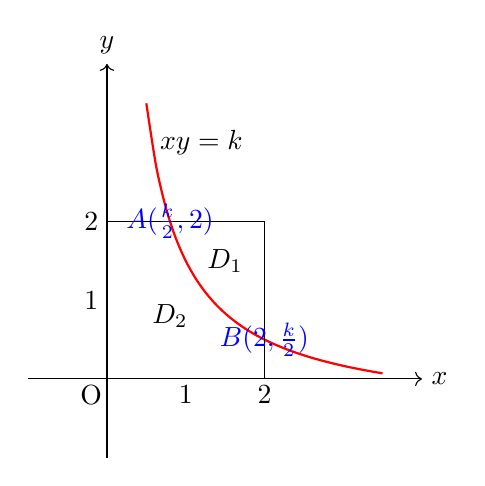
\begin{tikzpicture}
			\draw[->] (-1,0) -- (4,0) node[right] {$x$};
			\draw[->] (0,-1) -- (0,4) node[above] {$y$};
			\draw[red,thick, domain=0.5:3.5, smooth, variable=\x] plot ({\x},{2/\x-0.5});
			\draw(0,2) -- (2,2);
			\draw(2,0) -- (2,2);
			\node at (1,-0.2) {$1$};
			\node at (2,-0.2) {$2$};
			\node at (-0.2,1) {$1$};
			\node at (-0.2,2) {$2$};
			\node [blue] (A) at (0.8,2){$A(\frac{k}{2},2)$};
			\node [blue] (B) at (2,0.5){$B(2,\frac{k}{2})$};
			\node at (1.2,3) {$xy = k$}; 
			\node at (1.5,1.5) {$D_{1}$};
			\node at (0.8,0.8) {$D_{2}$};
			\node at (-0.2,-0.2) {O};
		\end{tikzpicture}
		\caption{积分区域图}
	\end{figure} 
	
	原二重积分等价于: 
	\begin{eqnarray*}
		I&=&\iint\limits_{D_{1}}(xy-k)dxdy+\iint\limits_{D_{2}}(k-xy)dxdy\\
		&=&\int_{\frac{k}{2}}^{2}dx\int_{\frac{k}{x}}^{2}(xy-k)dy+\int_{0}^{\frac{k}{2}}dx\int_{0}^{2}(k-xy)dy+\int_{\frac{k}{2}}^{2}dx\int_{0}^{\frac{k}{x}}(k-xy)dy\\
		&=&\dfrac{3}{4}k^2-4k+4+\dfrac{3}{4}k^2+k^2\ln 2-k^2\ln \frac{k}{2}\\
		&=&2k^2\ln 2-k^2\ln k+\dfrac{3}{2}k^2+4-4k
	\end{eqnarray*}
	
	我们得到: 
	$$\left\lbrace
	\begin{array}{l}
		2k^2=2\\
		\ln k=0\\
		\dfrac{3}{2}k^2+4-4k=\dfrac{3}{2}
	\end{array}
	\right. \Rightarrow k=1$$
	
	综上所述,我们找到$k=1$使得上式成立,我们有: $\exists (\xi,\eta)\in D,\ s.t. |f'(\xi,\eta)|\geq \dfrac{2}{4\ln 2+3}$
\end{solution}

\begin{example}[][Exam: 33.1.6]
	$$\lim\limits_{x\to+\infty}(x^{\frac{1}{x}}-1)^{\frac{1}{\ln x}}$$
\end{example}

\begin{solution}
	
	原极限等价于: 
	\begin{eqnarray*}
		I&=&\lim\limits_{x\to+\infty}e^{\dfrac{\ln(e^{\frac{\ln x}{x}}-1)}{\ln x}}\\
		&\overset{L}{=}&\lim\limits_{x\to+\infty}e^{\dfrac{(1-\ln x)e^{\frac{\ln x}{x}}}{x(e^{\frac{\ln x}{x}}-1)}}\\
		&=&\lim\limits_{x\to+\infty}e^{\dfrac{(1-\ln x)e^{\frac{\ln x}{x}}}{\ln x}}\\
		&=&e^{-1}
	\end{eqnarray*}
	\begin{anymark}[注]
		\begin{itemize}
			\item 如果$f\sim g$,我们有$\ln f\sim \ln g$
		\end{itemize}
	\end{anymark}
\end{solution}


\textcolor{orange}{July 4}

\begin{example}[][Exam: 33.1.7]
	已知 $a_{n}=\sum\limits_{k=1}^{n}\dfrac{1}{k^2}, b_{n}=\sum\limits_{k=1}^{n}\dfrac{1}{(2k-1)^2}$,
	且 $\lim\limits_{n\to +\infty}a_{n}=\dfrac{\pi^2}{6}$

(1). 证明: $a_{2n}=\dfrac{1}{4}a_{n}+b_{n}(n=1,2,\cdots)$

(2). $\lim\limits_{n\to+\infty}n\left(\dfrac{b_{n}}{a_{n}}-\dfrac{3}{4}\right) $
\end{example}
\begin{solution}
	
	(1). 我们有: $$\dfrac{1}{4}a_{n}=\dfrac{1}{4}\sum\limits_{k=1}^{n}\dfrac{1}{k^2}=\sum\limits_{k=1}^{n}\dfrac{1}{(2k)^2}$$
	
	因此,我们有: 
	\begin{eqnarray*}
		\dfrac{1}{4}a_{n}+b_{n}&=&\sum\limits_{k=1}^{n}\dfrac{1}{(2k)^2}+\sum\limits_{k=1}^{n}\dfrac{1}{(2k-1)^2}\\
		&=&\sum\limits_{k=1}^{2n}\dfrac{1}{k^2}\\
		&=&a_{2n}
	\end{eqnarray*}
	
	(2).原极限等价于: 
	\begin{eqnarray*}
		I&=&\lim\limits_{n\to+\infty}n\left( \dfrac{a_{2n}-a_{n}}{a_{n}}\right)\\
		&=&\dfrac{\lim\limits_{n\to+\infty}n(a_{2n}-a_{n})}{\lim\limits_{n\to+\infty}a_{n}}\\
		&=&\dfrac{6}{\pi^2}\lim\limits_{n\to+\infty}n\left[ \dfrac{1}{(n+1)^2}+\dfrac{1}{(n+2)^2}+\cdots+\dfrac{1}{(n+k)^2}+\cdots+\dfrac{1}{(n+n)^2}\right]\\
		&=& \dfrac{6}{\pi^2}\lim\limits_{n\to+\infty}\sum\limits_{k=1}^{n}\dfrac{1}{(1+\frac{k}{n})^2}\\
		&=&\dfrac{6}{\pi^2}(-\dfrac{1}{1+x})|_{0}^{1}\\
		&=&\dfrac{3}{\pi^2}
	\end{eqnarray*}
\end{solution}
\begin{anymark}[注]
	\begin{itemize}
		\item $\sum\limits_{n=1}^{+\infty}\dfrac{1}{n^2}=\dfrac{\pi^2}{6}$
		\item $\sum\limits_{n=1}^{+\infty}\dfrac{1}{(2n-1)^2}=\dfrac{\pi^2}{8}$
		\item $\sum\limits_{n=1}^{+\infty}\dfrac{1}{(2n)^2}=\dfrac{\pi^2}{24}$
	\end{itemize}
\end{anymark}

\begin{example}[][Exam: 33.1.8]
	$\lim\limits_{x\to 0}\dfrac{\cos(xe^x)-e^{-\frac{x^2}{2}e^{2x}}}{x^{\alpha}} = \beta\neq0$, 求 $\alpha,\beta$
\end{example}

\begin{solution}
	
	原极限等价于: 
	\begin{eqnarray*}
		I&=&\lim\limits_{x\to 0}\dfrac{1-\frac{1}{2}x^2e^{2x}+\frac{1}{24}x^4e^{4x}-(1-\frac{1}{2}x^2e^{2x}+\frac{1}{8}x^4e^{4x})}{x^{\alpha}}\\
		&=&\lim\limits_{x\to 0}\dfrac{-\frac{1}{12}x^4e^{4x}}{x^{\alpha}}\\
		&=&\beta
	\end{eqnarray*}
	
	我们得到: $\alpha=4,\ \beta=-\dfrac{1}{12}$
\end{solution}


\textcolor{orange}{July 5}

\begin{example}[][Exam: 33.1.9]
	$$\int_{0}^{+\infty}\dfrac{\ln x}{x^2+a^2}dx(a>0)$$
\end{example}

\begin{solution}
	
	原积分等价于: 
	\begin{eqnarray*}
		I&=&\dfrac{1}{a}\int_{0}^{+\infty}\dfrac{\ln a+\ln \frac{x}{a}}{(\frac{x}{a})^2+1}d(\frac{x}{a})\\
		&=&\dfrac{1}{a}\int_{0}^{+\infty}\dfrac{\ln a+\ln u}{u^2+1}du\\
		&=&\dfrac{\ln a}{a}\int_{0}^{+\infty}\dfrac{1}{u^2+1}du+\dfrac{1}{a}\int_{0}^{+\infty}\dfrac{\ln u}{u^2+1}du\\
		&=&I_{1}+I_{2}\\
		I_{1}&=&\dfrac{\pi \ln a}{2a}\\
		I_{2}&=&\dfrac{1}{a}\int_{0}^{+\infty}\dfrac{\ln u}{u^2+1}du=\dfrac{1}{a}\int_{+\infty}^{0}\dfrac{-\ln t }{(\frac{1}{t})^2+1}(-\dfrac{1}{t^2})dt=-\dfrac{1}{a}\int_{0}^{+\infty}\dfrac{\ln t}{t^2+1}dt\Rightarrow I_{2}=0\\
		I&=&I_{1}+I_{2}=\dfrac{\pi \ln a}{2a}
	\end{eqnarray*}
\end{solution}
\begin{anymark}[$\int_{0}^{+\infty}f(x)dx$积分技巧]
	\begin{itemize}
		\item 倒代换
		\item 分割为$\int_{0}^{1}f(x)+\int_{1}^{+\infty}f(x)dx$
		\item 利用正切三角换元法
	\end{itemize}
\end{anymark}

\begin{example}[][Exam: 33.1.10]
	$\lim\limits_{x\to 0}\dfrac{\cos 2x-\cos x\sqrt{\cos 2x}}{x^{\alpha}}=\beta\neq0$, 求 $\alpha,\beta$
\end{example}

\begin{solution}
	
	原极限等价于: 
	\begin{eqnarray*}
		I&=&\lim\limits_{x\to 0}\dfrac{\cos^2 2x-\cos^2 x\cos 2x}{(\cos x+\cos x\sqrt{\cos 2x})x^{\alpha}}\\
		&=&\lim\limits_{x\to 0}\dfrac{-\cos2x\sin^2 x}{(\cos x+\cos x\sqrt{\cos 2x})x^{\alpha}}\\
		&=&\lim\limits_{x\to 0}\dfrac{-\cos 2x}{\cos x+\cos x\sqrt{\cos 2x}}\lim\limits_{x\to 0}\dfrac{\sin^2 x}{x^{\alpha}}\\
		&=&-\dfrac{1}{2}\lim\limits_{x\to 0}\dfrac{\sin^2 x}{x^{\alpha}}\\
		&=&\beta
	\end{eqnarray*}
	
	我们可以得到: $\alpha=2,\ \beta=-\dfrac{1}{2}$
\end{solution}


\textcolor{orange}{July 6}

\begin{example}[][Exam: 33.1.11]
	设 $f(x)=\dfrac{1}{1+3x+9x^2}$, 求 $f^{(100)}(0)$
\end{example}

\begin{solution}
	
	我们可以得到: 
	$$f(x)=\dfrac{1-3x}{(1-3x)(1+3x+9x^2)}=\dfrac{1}{1-(3x)^3}-3x\dfrac{1}{1-(3x)^3}$$
	
	我们将$f(x)$在$x=0$处泰勒展开得到: 
	$$\left\lbrace
	\begin{array}{l}
		f(x)=a_{0}+a_{1}x+a_{2}x^2+\cdots+a_{100}x^{100}+\cdots+a_{n}x^{n}+\cdots\\
		f(x)=f(0)+f'(0)x+\dfrac{f''(0)}{2!}x^2+\cdots+\dfrac{f^{(100)}}{100!}x^{100}+\cdots
	\end{array}
	\right. \Rightarrow f^{(100)}(0)=a_{100}100!$$
	
	我们有: $$-1<x<1,\ 1+x+x^2+x^3+\cdots+x^n=\dfrac{1}{1-x}$$
	
	我们得到: 
	$$f(x)=\sum\limits_{n=0}^{+\infty}(3x)^{3n}-\sum\limits_{n=0}^{+\infty}(3x)^{3n+1}$$
	
	我们得到: $a_{100}=-3^{100}\Rightarrow f^{(100)}(0)=-3^{100}100!$
\end{solution}

\begin{example}[][Exam: 33.1.12]
	$\lim\limits_{x\to 0}\dfrac{ax^2+bx+1-e^{x^2-2x}}{x^2}=2$, 求 $a,b$
\end{example}

\begin{solution}
	
	原极限等价于: 
	\begin{eqnarray*}
		I&=&\lim\limits_{x\to 0}\dfrac{ax^2+bx+1-(1+x^2-2x+\frac{1}{2}(x^2-2x)^2)}{x^2}\\
		&=&\lim\limits_{x\to 0}\dfrac{(b+2)x+(a-3)x^2}{x^2}\\
		&=&a-3
	\end{eqnarray*}
	
	我们得到: $\left\lbrace
	\begin{array}{l}
		a-3=2\\
		b+2=0
	\end{array}
	\right. \Rightarrow \left\lbrace
	\begin{array}{l}
		a=5\\
		b=-2
	\end{array}
	\right. $
\end{solution}


\textcolor{orange}{July 7}

\begin{example}[][Exam: 33.1.13]
	$$\lim\limits_{x\to 0}\dfrac{n!x^n-\sin x\sin 2x\cdots\sin nx}{x^{n+2}}$$
\end{example}

\begin{solution}
	
	原极限等价于: 
	\begin{eqnarray*}
		I&=&n!\lim\limits_{x\to 0}\dfrac{1-\frac{\sin x\sin 2x\cdots\sin nx}{n!x^n}}{x^2}\\
		&=&n!\lim\limits_{x\to 0}\dfrac{1-\frac{\sin x}{x}\frac{\sin 2x}{2x}\cdots\frac{\sin nx}{nx}}{x^2}\\
		&=&-n!\lim\limits_{x\to 0}\dfrac{\ln(\frac{\sin x}{x}\frac{\sin 2x}{2x}\cdots\frac{\sin nx}{nx})}{x^2}\\
		&=&-n!\sum\limits_{k=1}^{n}\lim\limits_{x\to 0}\dfrac{\ln(1+\frac{\sin kx-kx}{kx})}{x^2}\\
		&=&n!\sum\limits_{k=1}^{n}\lim\limits_{x\to 0}\dfrac{kx-\sin kx}{kx^3}\\
		&=&n!\sum\limits_{k=1}^{n}(\dfrac{k^2}{6})\\
		&=&n!\dfrac{n(n+1)(2n+1)}{36}\\
		&=&\dfrac{n(2n+1)(n+1)!}{36}
	\end{eqnarray*}
\end{solution}

\begin{example}[][Exam: 33.1.14]
	$\lim\limits_{x\to 0}\left(\dfrac{\ln(x+\sqrt{x^2+1})+ax^2+bx^3}{x} \right)^{\frac{1}{x^2}}=e^2$, 求 $a,b$
\end{example}
\begin{solution}
	
	原极限等价于: 
	\begin{eqnarray*}
		I&=&\lim\limits_{x\to 0}e^{\dfrac{\ln(\frac{\ln(x+\sqrt{1+x^2})+ax^2+bx^3-x}{x}+1)}{x^2}}\\
		&=&\lim\limits_{x\to 0}e^{\dfrac{\ln(x+\sqrt{1+x^2})+ax^2+bx^3-x}{x^3}}\\
		&=&e^{\lim\limits_{x\to 0}\dfrac{x-\frac{1}{6}x^3+o(x^3)+ax^2+bx^3-x}{x^3}}\\
		&=&e^{\lim\limits_{x\to 0}\dfrac{(b-\frac{1}{6})x^3+o(x^3)+ax^2}{x^3}}\\
		&=&e^2
	\end{eqnarray*}
	
	我们得到: $\left\lbrace
	\begin{array}{l}
		b-\frac{1}{6}=2\\
		a=0
	\end{array}
	\right. \Rightarrow \left\lbrace
	\begin{array}{l}
		b=\dfrac{13}{6}\\
		a=0
	\end{array}
	\right. $
\end{solution}
\begin{anymark}[注]
	$x\to 0,\ x\sim \ln(x+\sqrt{x^2+1})$
	
	我们可以得到: 
	$$[\ln(x+\sqrt{x^2+1})]'=\dfrac{1}{\sqrt{1+x^2}}=(1+x^2)^{\frac{1}{2}}=1-\dfrac{1}{2}x^2+\dfrac{3}{8}x^3+\cdots$$
	
	我们可以得到: $\ln(x+\sqrt{1+x^2})$的泰勒展开式: 
	$$\ln(x+\sqrt{1+x^2})=x-\dfrac{1}{6}x^3+o(x^3)$$
\end{anymark}


\section{Week \Rmnum{2}}

\textcolor{blue}{July 8}

\begin{example}[][Exam: 33.2.1]
	设 $n$ 阶矩阵 $A,B$ 满足 $AB+aA+bB+cE=O$, 其中 $ab\neq c$, 证明: 

(1). $A+bE$ 与 $B+aE$ 均为可逆矩阵 

(2). $AB=BA$
\end{example}
1. 

\begin{solution}
	
	(1). 我们由$AB+aA+bB+cE=O$可以得到: 
	$$(A+bE)(B+aE)=(ab-c)E$$
	
	我们得到: $$\left\lbrace
	\begin{array}{l}
		\dfrac{1}{ab-c}(A+bE)(B+aE)=E\\
		(A+bE)\dfrac{1}{ab-c}(B+aE)=E
	\end{array}
	\right. $$
	
	我们得到: $A+bE$与$B+aE$均为可逆矩阵 
	
	(2). 我们可以得到: 
	$$\dfrac{1}{ab-c}(A+bE)(B+aE)=\dfrac{1}{ab-c}(B+aE)(A+bE)$$
	
	我们化简一下: 
	$$\left\lbrace
	\begin{array}{l}
		\text{左边}=AB+bB+aA+abE\\
		\text{右边}=BA+aA+bB+abE
	\end{array}
	\right. \Rightarrow AB=BA$$
\end{solution}

\begin{example}[][Exam: 33.2.2]
	已知常数 $a>0, bc\neq 0$, 且 $\lim\limits_{x\to+\infty}[x^a\ln(1+\frac{x}{b})-x]=c$, 求 $a,b,c$
\end{example}

\begin{solution}
	
	原极限等价于: 
	\begin{eqnarray*}
		I&=&\lim\limits_{x\to 0 }\dfrac{\ln(1+bx)-x^{a-1}}{x^a}\\
		&=&\lim\limits_{x\to 0 }\dfrac{bx-\frac{1}{2}b^2x^2-x^{a-1}}{x^a}\\
		&=&c
	\end{eqnarray*}
	
	我们得到: $\left\lbrace
	\begin{array}{l}
		a-1=1\\
		b=1\\
		c=-\dfrac{1}{2}b^2
	\end{array}
	\right. \Rightarrow \left\lbrace
	\begin{array}{l}
		a=2\\
		b=1\\
		c=-\dfrac{1}{2}
	\end{array}
	\right. $
\end{solution}


\textcolor{blue}{July 9}

\begin{example}[][Exam: 33.2.3]
	$$\lim\limits_{n\to +\infty}\dfrac{1}{n}\left[\int_{\frac{1}{3}}^{\frac{1}{6n}}\dfrac{\sin y}{y}dy+\int_{\frac{1}{3}}^{\frac{3}{6n}}\dfrac{\sin y}{y}dy+\cdots+\int_{\frac{1}{3}}^{\frac{(2n-1)}{6n}}\dfrac{\sin y}{y}dy \right]$$
\end{example}

\begin{solution}
	
	原极限等价于: 
	\begin{eqnarray*}
		I&=&\lim\limits_{n\to +\infty}\dfrac{1}{n}\sum\limits_{k=1}^{n}\int_{\frac{1}{3}}^{\frac{2k-1}{6n}}\dfrac{\sin y}{y}dy\\
		&=&\lim\limits_{n\to +\infty}\dfrac{1}{n}\sum\limits_{k=1}^{n}f(\frac{2k-1}{2n})\\
		&=&\int_{0}^{1}[\int_{\frac{1}{3}}^{\frac{1}{3}x}\dfrac{\sin y}{y}dy]dx\\
		&=&-\int_{0}^{\frac{1}{3}}dy\int_{0}^{3y}\dfrac{\sin y}{y}dx\\
		&=&-\int_{0}^{\frac{1}{3}}3\sin ydy\\
		&=&3(\cos \frac{1}{3}-1)
	\end{eqnarray*}
\end{solution}

\begin{example}[][Exam: 33.2.4]
	设 $A$ 为 $n$ 阶反对称矩阵, 证明: 对于任意向量 $x$, 均有 $x^{T}(A+E)x\geq 0$
\end{example}

\begin{solution}
	
	我们有: $$x^{T}(A+E)x=[x^{T}(A+E)x]^T=x^{T}(A^{T}+E)x=x^{T}(-A+E)x$$
	
	$$x^{T}(A+E)x+x^{T}(A-E)x=2x^{T}Ax=0\Rightarrow x^{T}(A+E)x=x^{T}Ax+x^{T}Ex=x^{T}x\geq 0$$
\end{solution}


\textcolor{blue}{July 10}

\begin{example}[][Exam: 33.2.5]
	$$\dfrac{n^{s+1}}{s+1} < 1^s+2^s+\cdots+n^s < \dfrac{(n+1)^{s+1}}{s+1} (s > 0)$$
\end{example}

\begin{figure}[H]
	\centering
	\subfigure[定积分定义示意图$\alpha$]{
		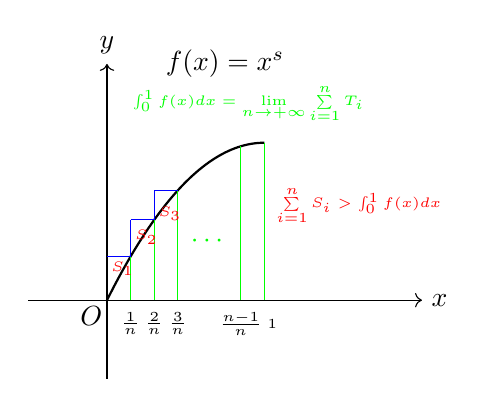
\begin{tikzpicture}
			\draw[->] (-1,0) -- (4,0) node[right] {$x$};
			\draw[->] (0,-1) -- (0,3) node[above] {$y$};
			\draw[thick, domain=0:2, smooth, variable=\x] plot ({\x},{-0.5*\x*\x+2*\x});
			\draw[green] (0.3,0) -- (0.3,0.555);
			\draw[green] (0.6,0) -- (0.6,1.02);
			\draw[green] (0.9,0) -- (0.9,1.395);
			\draw[green] (1.7,0) -- (1.7,1.955);
			\draw[green] (2,0) -- (2,2);
			\draw[blue] (0,0.555) -- (0.3,0.555);
			\draw[blue] (0.3,0.555) -- (0.3,1.02);
			\draw[blue] (0.3,1.02) -- (0.6,1.02);
			\draw[blue] (0.6,1.02) -- (0.6,1.395);
			\draw[blue] (0.6,1.395) -- (0.9,1.395);
			\node[green] at (1.3,0.75) {$\cdots$};
			\node at (0.3,-0.3) {\tiny{$\frac{1}{n}$}};
			\node at (0.6,-0.3) {\tiny{$\frac{2}{n}$}};
			\node at (0.9,-0.3) {\tiny{$\frac{3}{n}$}};
			\node at (1.7,-0.3) {\tiny{$\frac{n-1}{n}$}};
			\node at (2.1,-0.3) {\tiny{$1$}};
			\node at (-0.2,-0.2) {$O$};
			\node at (1.5,3) {$f(x) = x^{s}$};
			\node[red] at (0.2,0.4) {\tiny{$S_{1}$}};
			\node[red] at (0.5,0.8) {\tiny{$S_{2}$}};
			\node[red] at (0.8,1.1) {\tiny{$S_{3}$}};
			\node[green] at (1.8,2.5) {\tiny{$\int_{0}^{1}f(x) dx=\lim\limits_{n\to +\infty}\sum\limits_{i=1}^{n}T_{i}$}};
			\node[red] at (3.2,1.2) {\tiny{$\sum\limits_{i=1}^{n}S_{i} > \int_{0}^{1}f(x)dx$}};
		\end{tikzpicture}	
	}
	\subfigure[定积分定义示意图$\beta$]{
		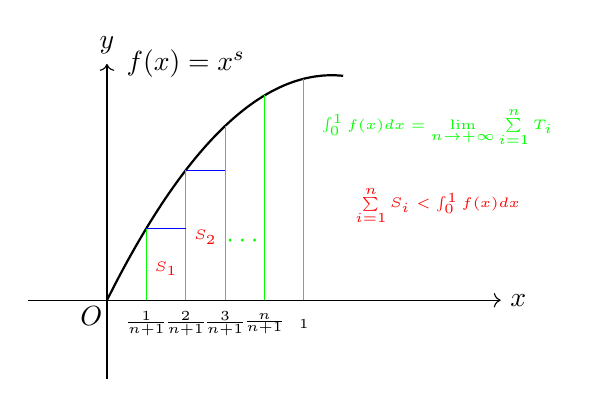
\begin{tikzpicture}
			\draw[->] (-1,0) -- (5,0) node[right] {$x$};
			\draw[->] (0,-1) -- (0,3) node[above] {$y$};
			\draw[thick, domain=0:3, smooth, variable=\x] plot ({\x},{-0.35*\x*\x+2*\x});
			\draw[green] (0.5,0) -- (0.5,0.9125);
			\draw[green] (1,0) -- (1,1.65);
			\draw[green] (1.5,0) -- (1.5,2.2125);
			\draw[green] (2,0) -- (2,2.6);
			\draw[green] (2.5,0) -- (2.5,2.8125);
			\draw[blue] (0.5,0.9125) -- (1,0.9125);
			\draw[blue] (1,1.65) -- (1.5,1.65);
			\node[green] at (1.75,0.75) {$\cdots$};
			\node at (0.5,-0.3) {\tiny{$\frac{1}{n+1}$}};
			\node at (1,-0.3) {\tiny{$\frac{2}{n+1}$}};
			\node at (1.5,-0.3) {\tiny{$\frac{3}{n+1}$}};
			\node at (2,-0.3) {\tiny{$\frac{n}{n+1}$}};
			\node at (2.5,-0.3) {\tiny{$1$}};
			\node at (-0.2,-0.2) {$O$};
			\node at (1,3) {$f(x) = x^{s}$};
			\node[red] at (0.75,0.4) {\tiny{$S_{1}$}};
			\node[red] at (1.25,0.8) {\tiny{$S_{2}$}};
			\node[green] at (4.2,2.2) {\tiny{$\int_{0}^{1}f(x) dx=\lim\limits_{n\to +\infty}\sum\limits_{i=1}^{n}T_{i}$}};
			\node[red] at (4.2,1.2) {\tiny{$\sum\limits_{i=1}^{n}S_{i} < \int_{0}^{1}f(x)dx$}};
		\end{tikzpicture}
		}
	\caption{积分和求和关系图}
\end{figure} 
\begin{solution}
	
	原不等式可以化为: 
	$$\left\lbrace
	\begin{array}{l}
		\dfrac{1}{n}[(\frac{1}{n})^s+(\frac{2}{n})^s+\cdots+(\frac{n}{n})^s]>\dfrac{1}{s+1}\\
		\dfrac{1}{n+1}[(\frac{1}{n+1})^s+(\frac{2}{n+1})^s+\cdots+(\frac{n}{n+1})^s]<\dfrac{1}{s+1}
	\end{array}
	\right. $$
	
	如图$(a)$第一个不等式: 
	$$\text{左边}=\sum\limits_{i=1}^{n}S_{i}>\int_{0}^{1}x^sdx=\dfrac{1}{s+1}=\text{右边}$$
	
	如图$(b)$第二个不等式: 
	$$\text{左边}=\sum\limits_{i=1}^{n}S_{i}<\int_{0}^{1}x^sdx=\dfrac{1}{s+1}=\text{右边}$$
\end{solution}

\begin{example}[][Exam: 33.2.6]
	$$\lim\limits_{n\to +\infty}\dfrac{1^{p+1}+2^{p+1}+\cdots+n^{p+1}}{n(1^p+2^p+\cdots+n^p)}(p>0)$$
\end{example}

\begin{solution}
	
	原极限等价于: 
	\begin{eqnarray*}
		I&=&\lim\limits_{n\to +\infty}\dfrac{(\frac{1}{n})^{p+1}+(\frac{2}{n})^{p+1}+\cdots+(\frac{n}{n})^{p+1}}{(\frac{1}{n})^{p}+(\frac{2}{n})^{p}+\cdots+(\frac{n}{n})^{p}}\\
		&=&\lim\limits_{n\to +\infty}\dfrac{\frac{1}{n}[(\frac{1}{n})^{p+1}+(\frac{2}{n})^{p+1}+\cdots+(\frac{n}{n})^{p+1}]}{\frac{1}{n}[(\frac{1}{n})^{p}+(\frac{2}{n})^{p}+\cdots+(\frac{n}{n})^{p}]}\\
		&=&\lim\limits_{n\to +\infty}\dfrac{\frac{1}{n}\sum\limits_{k=1}^{n}(\frac{k}{n})^{p+1}}{\frac{1}{n}\sum\limits_{k=1}^{n}(\frac{k}{n})^{p}}\\
		&=&\dfrac{\int_{0}^{1}\dfrac{x^{p+2}}{p+2}dx}{\int_{0}^{1}\dfrac{x^{p+1}}{p+1}dx}\\
		&=&\dfrac{p+1}{p+2}
	\end{eqnarray*}
\end{solution}


\textcolor{blue}{July 11}

\begin{example}[][Exam: 33.2.7]
	已知 $ A = 
	\begin{bmatrix}
		0 & -1 & 1\\
		2 & -3 & 0\\
		0 &  0 & 0
	\end{bmatrix}$, 求 $A^{99}$
\end{example}

\begin{solution}
	
	我们将矩阵$A$相似对角化: 
	
	(1). 求矩阵$A$的特征值和特征向量
	
	$$\left| \lambda E-A\right|=\left| \begin{matrix}
		\lambda&1&-1\\-2&\lambda+3&0\\
		0&0&\lambda
	\end{matrix}\right|=\lambda(\lambda+1)(\lambda+2)$$
	
	矩阵$A$的特征值为$\lambda_{1}=0,\ \lambda_{2}=-1,\ \lambda_{3}=-2$
	
	当$\lambda_{1}=0$时,$(-A)x=0\Rightarrow \left[ \begin{matrix}
		0&1&-1\\
		-2&3&0\\
		0&0&0
	\end{matrix}\right]\left[ \begin{matrix}
		x_{1}\\x_{2}\\x_{3}
	\end{matrix}\right]=0\Rightarrow \xi_{1}=(3,2,2)^T$
	
	当$\lambda_{2}=-1$时,$(-E-A)x=0\Rightarrow \left[ \begin{matrix}
		-1&1&-1\\
		-2&2&0\\
		0&0&-1
	\end{matrix}\right]\left[ \begin{matrix}
		x_{1}\\x_{2}\\x_{3}
	\end{matrix}\right]=0\Rightarrow \xi_{2}=(1,1,0)^T$
	
	当$\lambda_{3}=-2$时,$(-2E-A)x=0\Rightarrow \left[ \begin{matrix}
		-2&1&-1\\
		-2&1&0\\
		0&0&-2
	\end{matrix}\right]\left[ \begin{matrix}
		x_{1}\\x_{2}\\x_{3}
	\end{matrix}\right]=0\Rightarrow \xi_{3}=(1,2,0)^T$
	
	存在可逆矩阵$P=\left[ \begin{matrix}
		3&1&1\\2&1&2\\2&0&0
	\end{matrix}\right]$,$\ s.t. \ P^{-1}AP=\varLambda=\left[ \begin{matrix}
		0& & \\ &-1& \\ & &-2
	\end{matrix}\right]$,其中$P^{-1}=\left[ \begin{matrix}
		0&0&\frac{1}{2}\\2&-1&-2\\-1&1&\frac{1}{2}
	\end{matrix}\right]$
	
	我们得到: $$A=P\varLambda P^{-1}\Rightarrow A^{99}=P\varLambda^{99}P^{-1}$$
	
	上面的式子可以化为: 
	\begin{eqnarray*}
		A^{99}&=&\left[ \begin{matrix}
			3&1&1\\2&1&2\\2&0&0
		\end{matrix}\right]\left[ \begin{matrix}
			0& & \\ &-1& \\ & &-2^{99}
		\end{matrix}\right]\left[ \begin{matrix}
			0&0&\frac{1}{2}\\2&-1&-2\\-1&1&\frac{1}{2}
		\end{matrix}\right]\\
		&=&\left[ \begin{matrix}
			0&-1&-2^{99}\\0&-1&-2^{100}\\0&0&0
		\end{matrix}\right]\left[ \begin{matrix}
			0&0&\frac{1}{2}\\2&-1&-2\\-1&1&\frac{1}{2}
		\end{matrix}\right]\\
		&=&\left[ \begin{matrix}
			2^{99}-2&1-2^{99}&2-2^{98}\\2^{100}-2&1-2^{100}&2-2^{99}\\0&0&0
		\end{matrix}\right]
	\end{eqnarray*}
\end{solution}

\begin{example}[][Exam: 33.2.8]
	设 $3$ 阶实对称矩阵 $A$ 特征值为 $\lambda_{1}=-1, \lambda_{2}=\lambda_{3}=1, \lambda_{1}$ 的特征向量为 $\xi_{1}=[0,1,1]^{T}$, 求 $A$
\end{example}

\begin{solution}
	
	我们不妨设特征值$\lambda_{2},\ \lambda_{3}$对应的特征向量为$x=(x_{1},x_{2},x_{3})^T$,我们由实对称矩阵不同特征值对应的特征向量相互正交得到: 
	$$x_{2}+x_{3}=0$$
	
	我们不妨取$\xi_{2}=(1,0,0)^T,\ \xi_{3}=(0,-1,1)^T$作为特征值$\lambda_{2},\ \lambda_{3}$的特征向量.我们将$\xi_{1},\xi_{2},\xi_{3}$单位化得到: 
	$$\left\lbrace
	\begin{array}{l}
		\eta_{1}=(0,\frac{1}{\sqrt{2}},\frac{1}{\sqrt{2}})^T\\
		\eta_{2}=(1,0,0)^T\\
		\eta_{3}=(0,-\frac{1}{\sqrt{2}},\frac{1}{\sqrt{2}})^T
	\end{array}
	\right. $$
	
	我们得到: $$\exists \text{可逆矩阵}P=[\eta_{1},\eta_{2},\eta_{3}
	],\ s.t. P^{-1}AP=\varLambda=\left[ \begin{matrix}
		-1& & \\ &1& \\ & &1
	\end{matrix}\right]$$
	
	其中$P=\left[ \begin{matrix}
		0&1&0\\ \frac{1}{\sqrt{2}}&0&-\frac{1}{\sqrt{2}} \\\frac{1}{\sqrt{2}}&0&\frac{1}{\sqrt{2}}
	\end{matrix}\right]$,$P^{-1}=\left[ \begin{matrix}
		0&\frac{1}{\sqrt{2}}&\frac{1}{\sqrt{2}}\\ 1&0&0 \\0&-\frac{1}{\sqrt{2}}&\frac{1}{\sqrt{2}}
	\end{matrix}\right]$
	
	我们得到: 
	\begin{eqnarray*}
		A&=&P\varLambda P^{-1}\\
		&=&\left[ \begin{matrix}
			0&1&0\\ 1&0&-1 \\1&0&2
		\end{matrix}\right]\left[ \begin{matrix}
			-1& & \\ &1& \\ & &1
		\end{matrix}\right]\left[ \begin{matrix}
			0&\frac{1}{\sqrt{2}}&\frac{1}{\sqrt{2}}\\ 1&0&0 \\0&-\frac{1}{\sqrt{2}}&\frac{1}{\sqrt{2}}
		\end{matrix}\right]\\
		&=&\left[ \begin{matrix}
			1&0&0\\ 0&0&-1 \\0&-1&0
		\end{matrix}\right]
	\end{eqnarray*}
\end{solution}


\textcolor{blue}{July 12}

\begin{example}[][Exam: 33.2.9]
	设 $A$ 是任意的 $m\times n$ 矩阵, 证明: 方程组 $A^{T}Ax=A^{T}b$ 一定有解
\end{example}

\begin{solution}
	
	我们知道非齐次方程组有解的充要条件为: $rank(A)=rank([A,b])$
	
	在此题中,我们需要证明: $$rank(A^TA)=rank([A^TA,A^Tb])=rank(A^T[A,b])$$
	
	显然,我们由$rank(AB)\leq min\{rank(A),rank(B)\}$有: 
	$$rank(A^TA)\leq rank([A^TA,A^Tb])=rank(A^T[A,b])\leq rank(A^T)$$
	
	我们还有: $rank(A)=rank(A^T)=rank(AA^T)=rank(A^TA)$
	
	因此我们得到: 
	$$\left\lbrace
	\begin{array}{l}
		rank(A^TA)=rank(A)\leq rank([A^TA,A^Tb])\\
		rank([A^TA,A^Tb])\geq rank(A^T)=rank(A)=rank(A^TA)
	\end{array}
	\right. \Rightarrow rank(A^TA)=rank([A^TA,A^Tb])$$
	
	原方程组一定有解.
\end{solution}

\begin{example}[][Exam: 33.2.10]
	设 $A$ 为 $3$ 阶实对称矩阵, $B = 
	\begin{pmatrix}
		3 & 0 & 0\\
		0 & 1 & 1\\
		0 & 0 & 1
	\end{pmatrix}, \alpha=(1,0,1)^{T}$ 是矩阵 $A$ 特征值 $3$ 的一个特征向量, 若 $r(3E-A)>1$, 且 $A^2-4E+3E=0$, 下列选项错误的是: 
	\begin{itemize}
		\item A. 矩阵 $A$ 必可相似对角化
		\item B. 矩阵 $B$ 不可以相似对角化
		\item C. 矩阵方程 $AX-XB=0$ 有可逆解
		\item D. $r(3E-A)=2$
	\end{itemize}
\end{example}

\begin{solution}
	
	A. 我们由实对称矩阵必可相似对角化得到矩阵$A$一定可以相似对角化.
	
	B. 矩阵$B$的三个特征值为$\lambda_{1}=3,\lambda_{2}=\lambda_{3}=1$,对于特征值$\lambda_{2}=\lambda_{3}=1$,$n-r(E-B)=1$,不满足相似对角化条件.
	
	C. 假设方程$AX-XB=0$存在可逆解,我们有$AXX^{-1}=XBX^{-1}\Rightarrow A=XBX^{-1}$,我们可以得到: $A\sim B$,我们有$A\sim\varLambda$,可以得到: $B\sim\varLambda$,矛盾!!
	
	D. 我们有: $A^2-4E+3E=0\Rightarrow (A-3E)(A-E)=0$,矩阵$A$的特征值有$\lambda_{1}=3,\lambda_{2}=1$,对应$r(3E-A)=1\text{或者}2$,又因为$r(3E-A)>1\Rightarrow r(3E-A)=2$.
\end{solution}


\textcolor{blue}{July 13}

\begin{example}[][Exam: 33.2.11]
	求 $f(x)=\sqrt{4x^2+x}\ln(2+\dfrac{1}{x})$ 的斜渐近线
\end{example}

\begin{solution}
	
	我们不妨假设$f(x)$的斜渐近线为$y=ax+b$,我们得到: 
	
	(1).
	$$\left\lbrace
	\begin{array}{l}
		a=\lim\limits_{x\to+\infty}\dfrac{f(x)}{x}\\
		b=\lim\limits_{x\to+\infty}(f(x)-ax)
	\end{array}
	\right. $$
	
	我们得到: 
	$$\left\lbrace
	\begin{array}{l}
		a=\lim\limits_{x\to+\infty}\sqrt{4+\dfrac{1}{x}}\ln(2+\dfrac{1}{x})=2\ln 2\\
		b=\lim\limits_{x\to+\infty}[\sqrt{4x^2+x}\ln(2+\dfrac{1}{x})-2\ln 2 x]=\lim\limits_{t\to 0^{+}}\dfrac{\sqrt{4+t}\ln(2+t)-2\ln 2}{t}=\lim\limits_{t\to 0^{+}}(\dfrac{\ln(2+t)}{2\sqrt{4+t}}+\dfrac{\sqrt{4+t}}{t+2})=\dfrac{\ln 2}{4}+1
	\end{array}
	\right. $$
	
	(2). 
	$$\left\lbrace
	\begin{array}{l}
		a=\lim\limits_{x\to-\infty}\dfrac{f(x)}{x}\\
		b=\lim\limits_{x\to-\infty}(f(x)-ax)
	\end{array}
	\right. $$
	
	我们得到: 
	$$\left\lbrace
	\begin{array}{l}
		a=\lim\limits_{x\to-\infty}-\sqrt{4+\dfrac{1}{x}}\ln(2+\dfrac{1}{x})=-2\ln 2\\
		b=\lim\limits_{x\to-\infty}[\sqrt{4x^2+x}\ln(2+\dfrac{1}{x})+2\ln 2 x]=\lim\limits_{t\to 0^{-}}\dfrac{2\ln 2-\sqrt{4+t}\ln(2+t)}{t}=-\dfrac{\ln 2}{4}-1
	\end{array}
	\right. $$
	
	综上所述,$f(x)$的斜渐近线为$y=2\ln 2 \ x+\dfrac{\ln 2}{4}+1$和$y=-2\ln 2 \ x-\dfrac{\ln 2}{4}-1$
	
	\begin{anymark}[注]
		利用泰勒展开式来求渐近线.
		
		$f(x)=\sqrt{4x^2+x}\ln(2+\frac{1}{x})$,我们利用泰勒展开式得到: 
		$$\left\lbrace
		\begin{array}{l}
			x\to +\infty,\ f(x)\sim 2x\sqrt{1+\frac{1}{4x}}[\ln2+\ln(1+\frac{1}{2x})]=2x(1+\frac{1}{8x})(\ln 2+\frac{1}{2x})=2\ln 2\ x+\frac{\ln 2}{4}+1\\
			x\to -\infty,\ f(x)\sim -2x\sqrt{1+\frac{1}{4x}}[\ln2+\ln(1+\frac{1}{2x})]=-2x(1+\frac{1}{8x})(\ln 2+\frac{1}{2x})=-2\ln 2\ x-\frac{\ln 2}{4}-1\\
		\end{array}
		\right. $$
	\end{anymark}
\end{solution}

\begin{example}[][Exam: 33.2.12]
	当 $x\to 0$ 时,下列无穷小量最高阶的是: 
\begin{itemize}
	\item A. $(1+x)^{x^2}-1$
	\item B. $e^{x^4-2x}-1$
	\item C. $\int_{0}^{x^2}\sin t^2dt$
	\item D. $\sqrt{1+2x}-\sqrt[3]{1+3x}$
\end{itemize}
\end{example}

\begin{solution}
	
	A. $e^{x^2\ln(1+x)}-1\sim x^2\ln(1+x)\sim x^3\Rightarrow \text{最高阶} 3\text{阶}$
	
	B. $e^{x^4-2x}-1\sim x^4-x^2\Rightarrow \text{最高阶} 4\text{阶}$
	
	C. $\int_{0}^{x^2}\sin t^2dt\sim \dfrac{x^6}{3}\Rightarrow \text{最高阶} 6\text{阶}$
	
	D. $\sqrt{1+2x}-\sqrt[3]{1+3x}=1+\dfrac{1}{2}2x-\dfrac{1}{8}(2x)^2-[1+\dfrac{1}{3}3x-\dfrac{1}{27}(3x^2)]\sim \dfrac{1}{12}x^2\Rightarrow \text{最高阶} 2\text{阶}$
\end{solution}


\textcolor{blue}{July 14}

\begin{example}[][Exam: 33.2.13]
	求曲线 $y=\sqrt{x^4-3x^3+4}$ 在 $x\to +\infty$ 方向的渐进二次曲线
\end{example}
\begin{solution}
	\begin{eqnarray*}
		\text{当}x\to +\infty,\ f(x)&=&x^2\sqrt{1+\dfrac{4-3x^3}{x^4}}\\
		&=&x^2[1+\dfrac{4-3x^3}{2x^4}-\dfrac{(4-3x^3)^2}{8x^8}]\\
		&=&x^2-\dfrac{3}{2}x-\dfrac{9}{8}+o(\dfrac{1}{x})
	\end{eqnarray*}
	
	原函数的渐近二次曲线为: $y=x^2-\dfrac{3}{2}x-\dfrac{9}{8}$
\end{solution}

\begin{example}[][Exam: 33.2.14]
	设 $\alpha_{1},\alpha_{2},\cdots,\alpha_{n}$ 是 $n$ 个 $n$ 维列向量, 证明: $\alpha_{1},\alpha_{2},\cdots,\alpha_{n}$ 线性无关的充要条件为: 
	$$\begin{vmatrix}
		\alpha_{1}^{T}\alpha_{1}&\alpha_{1}^{T}\alpha_{2}&\cdots&\alpha_{1}^{T}\alpha_{n}\\
		\alpha_{2}^{T}\alpha_{1}&\alpha_{2}^{T}\alpha_{2}&\cdots&\alpha_{2}^{T}\alpha_{n}\\
		\vdots&\vdots& &\vdots\\
		\alpha_{n}^{T}\alpha_{1}&\alpha_{n}^{T}\alpha_{2}&\cdots&\alpha_{n}^{T}\alpha_{n}
	\end{vmatrix}\neq 0$$
\end{example}

\begin{solution}
	
	我们不妨设$A=(\alpha_{1},\alpha_{2},\cdots,\alpha_{n})$,$A^{T}=\left( \begin{matrix}
		\alpha_{1}^{T}\\\alpha_{2}^{T}\\\cdots\\\alpha_{n}^{T}
	\end{matrix}\right) $,我们可以得到: 
	$$|AA^{T}|=\left| \begin{matrix}
		\alpha_{1}^{T}\alpha_{1}&\alpha_{1}^{T}\alpha_{2}&\cdots&\alpha_{1}^{T}\alpha_{n}\\\alpha_{2}^{T}\alpha_{1}&\alpha_{2}^{T}\alpha_{2}&\cdots&\alpha_{2}^{T}\alpha_{n}\\\vdots&\vdots& &\vdots\\\alpha_{n}^{T}\alpha_{1}&\alpha_{n}^{T}\alpha_{2}&\cdots&\alpha_{n}^{T}\alpha_{n}
	\end{matrix}\right|\Rightarrow |A|^2=\left| \begin{matrix}
		\alpha_{1}^{T}\alpha_{1}&\alpha_{1}^{T}\alpha_{2}&\cdots&\alpha_{1}^{T}\alpha_{n}\\\alpha_{2}^{T}\alpha_{1}&\alpha_{2}^{T}\alpha_{2}&\cdots&\alpha_{2}^{T}\alpha_{n}\\\vdots&\vdots& &\vdots\\\alpha_{n}^{T}\alpha_{1}&\alpha_{n}^{T}\alpha_{2}&\cdots&\alpha_{n}^{T}\alpha_{n}
	\end{matrix}\right|$$
	
	$\alpha_{1},\alpha_{2},\cdots,\alpha_{n}$线性无关等价于$|A|\neq 0$,证毕!
\end{solution}


\section{Week \Rmnum{3}}

\textcolor{cyan}{July 15}

\begin{example}[][Exam: 33.3.1]
	当 $x\to 0^{+}$ 时,下列无穷小量中最高阶的是: 
\begin{itemize}
	\item A. $\int_{0}^{1-\cos x}\dfrac{\sin t}{t}dt$
	\item B. $\int_{0}^{x}t\tan \sqrt{x^2-t^2}dt$
	\item C. $\int_{\sin x}^{1-\sqrt{\cos x}}e^{xt}\ln(1+t^3)dt$
	\item D. $\int_{\sin x}^{x}\sqrt{\sin^3 t}dt$
\end{itemize}
\end{example}

\begin{solution}
	
	A. $\int_{0}^{1-\cos x}\dfrac{\sin t}{t}dt\sim \int_{0}^{\frac{1}{2}x^2}1dt\sim \dfrac{1}{2}x^2\Rightarrow \text{最高阶} 2\text{阶}$
	
	B. 我们进行换元$u=x^2-t^2,d(t^2)=-du$,原积分等价于: $\int_{0}^{x^2}\dfrac{tan \sqrt{u}}{2}du\sim \dfrac{1}{3}x^3\Rightarrow \text{最高阶} 3\text{阶}$
	
	C. 我们可以得到原积分等价于: $\int_{\sin x}^{1-\sqrt{\cos x}}e^{xt}\ln(1+t^3)dt=I_{1}-I_{2}$
	$$I_{1}=\int_{0}^{1-\sqrt{\cos x}}e^{xt}\ln(1+t^3)dt$$
	$$I_{2}=\int_{0}^{\sin x}e^{xt}\ln(1+t^3)dt$$
	
	由积分中值定理得到: 
	
	$I_{1}=e^{x\xi}\int_{0}^{1-\sqrt{\cos x}}\ln(1+t^3)dt\sim \dfrac{1}{4^5}x^8\Rightarrow \text{最高阶} 8\text{阶}$
	
	$I_{2}=e^{x\xi}\int_{0}^{\sin x}\ln(1+t^3)dt\sim \dfrac{1}{4}x^4\Rightarrow \text{最高阶} 4\text{阶}$
	
	$\int_{\sin x}^{1-\sqrt{\cos x}}e^{xt}\ln(1+t^3)dt\sim\dfrac{1}{4}x^4\Rightarrow \text{最高阶} 4\text{阶}$
	
	D. 由积分中值定理得到: 
	$$\int_{\sin x}^{x}\sqrt{\sin^3 t}dt=(x-\sin x)\sin^{\frac{3}{2}}\xi\sim \dfrac{1}{6}x^{\frac{9}{2}},\ \xi\in(\sin x,x)\Rightarrow \text{最高阶} \dfrac{9}{2}\text{阶}$$
\end{solution}

\begin{example}[][Exam: 33.3.2]
	$$\sum\limits_{n=1}^{+\infty}\dfrac{(-1)^n}{(2n-1)(2n+1)}$$
\end{example}

\begin{solution}
	
	我们可以得到: $\sum\limits_{n=1}^{+\infty}\dfrac{(-1)^n}{(2n-1)(2n+1)}=\dfrac{1}{2}\sum\limits_{n=1}^{+\infty}\dfrac{(-1)^n}{2n-1}-\dfrac{1}{2}\sum\limits_{n=1}^{+\infty}\dfrac{(-1)^n}{2n+1}$
	
	我们有: 
	$$\arctan x=\sum\limits_{n=0}^{+\infty}\dfrac{(-1)^nx^{2n+1}}{2n+1}\Rightarrow \dfrac{\pi}{4}=1-\dfrac{1}{3}+\dfrac{1}{5}+\cdots+\dfrac{(-1)^n}{2n+1}+\cdots$$
	
	我们不妨设$S=\sum\limits_{n=1}^{+\infty}\dfrac{(-1)^n}{2n-1},\ T=\sum\limits_{n=1}^{+\infty}\dfrac{(-1)^n}{2n+1}$,我们有: 
	\begin{eqnarray*}
		\sum\limits_{n=1}^{+\infty}\dfrac{(-1)^n}{(2n-1)(2n+1)}&=&\dfrac{1}{2}(S-T)\\
		&=&\dfrac{1}{2}(-1+\dfrac{1}{3}-\dfrac{1}{5}+\cdots+\dfrac{(-1)^n}{2n-1}+\cdots)-\dfrac{1}{2}(-\dfrac{1}{3}+\dfrac{1}{5}+\cdots+\dfrac{(-1)^n}{2n+1}+\cdots)\\
		&=&-\dfrac{\pi}{8}-\dfrac{1}{2}(\dfrac{\pi}{4}-1)\\
		&=&\dfrac{1}{2}-\dfrac{\pi}{4}
	\end{eqnarray*}
	
\end{solution}

\begin{theorem}[常用泰勒级数]
	\begin{itemize}
		\item $$e^{x}=1+x+\dfrac{x^2}{2!}+\cdots+\dfrac{x^n}{n!}+\cdots=\sum\limits_{n=0}^{+\infty}\dfrac{x^n}{n!},\ x\in \mathbb{R}$$
		\item $$\text{欧拉公式: }e^{i\theta}=\cos\theta+i\sin\theta$$
	\end{itemize}
	\begin{eqnarray*}
		e^{i\theta} & = & 1+i\theta+\dfrac{(i\theta)^2}{2!}+\dfrac{(i\theta)^3}{3!}+\cdots+\dfrac{(i\theta)^n}{n!}+\cdots\\
		            & = & [1-\frac{\theta^2}{2!}+\frac{\theta^4}{4!}+\cdots+\frac{(-1)^{k}\theta^{2k}}{2k}+\cdots]+i[\theta-\dfrac{\theta^3}{3!}+\dfrac{\theta^5}{5!}+\cdots+\dfrac{(-1)^{k}\theta^{2k+1}}{(2k+1)!}+\cdots]\\
		            & = & \sum\limits_{n=0}^{+\infty}\dfrac{(-1)^{n}\theta^{2n}}{(2n)!}+i\sum\limits_{n=0}^{+\infty}\dfrac{(-1)^{n}\theta^{2n+1}}{(2n+1)!}
	\end{eqnarray*}
	\begin{itemize}
		\item $$\cos x=1-\dfrac{x^2}{2!}+\dfrac{x^4}{4!}+\cdots+\dfrac{(-1)^{n}x^{2n}}{(2n)!}+\cdots=\sum\limits_{n=0}^{+\infty}\dfrac{(-1)^{n}x^{2n}}{(2n)!},\ x\in\mathbb{R}$$
		\item $$\sin x=x-\dfrac{x^3}{3!}+\dfrac{x^5}{5!}+\cdots+\dfrac{(-1)^{n}x^{2n+1}}{(2n+1)!}+\cdots=\sum\limits_{n=0}^{+\infty}\dfrac{(-1)^{n}x^{2n+1}}{(2n+1)!},\ x\in\mathbb{R}$$
		\item $$\dfrac{1}{1-x}=1+x+x^2+\cdots+x^n+\cdots=\sum\limits_{n=0}^{+\infty}x^n,\ x\in(-1,1)$$
		\item $$\dfrac{1}{1+x}=1-x+x^2+\cdots+(-1)^nx^n+\cdots=\sum\limits_{n=0}^{+\infty}(-1)^nx^n,\ x\in(-1,1)$$
		\item $$\ln(1+x)=\int_{0}^{x}\dfrac{1}{1+x}dx=x-\dfrac{x^2}{2}+\dfrac{x^3}{3}+\cdots+\dfrac{(-1)^{n}x^{n+1}}{n+1}+\cdots=\sum\limits_{n=0}^{+\infty}\dfrac{(-1)^{n}x^{n+1}}{n+1},\ x\in(-1,1]$$
		\item 
		$$\ln(1-x)=-\int_{0}^{x}\dfrac{1}{1-x}dx=-[x+\dfrac{x^2}{2}+\dfrac{x^3}{3}+\cdots+\dfrac{x^{n+1}}{n+1}+\cdots]=-\sum\limits_{n=0}^{+\infty}\dfrac{x^{n+1}}{n+1},\ x\in[-1,1)$$
	\end{itemize}
\end{theorem}
\begin{proposition}[扩展泰勒级数]
	\begin{itemize}
		\item $$\dfrac{1}{1+x^2}=1-x^2+x^4+\cdots+(-1)^nx^{2n}+\cdots=\sum\limits_{n=0}^{+\infty}(-1)^nx^{2n},\ x\in(-1,1)$$
		\item $$\arctan x=\int_{0}^{x}\dfrac{1}{1+x^2}dx=x-\dfrac{x^3}{3}+\dfrac{x^5}{5}+\cdots+\dfrac{(-1)^{n}x^{2n+1}}{2n+1}+\cdots=\sum\limits_{n=0}^{+\infty}\dfrac{(-1)^{n}x^{2n+1}}{2n+1},\ x\in[-1,1]$$
		\item $$(1+x)^{\alpha}=1+\alpha x+\dfrac{\alpha(\alpha-1)}{2!}x^2+\cdots+\dfrac{\alpha(\alpha-1)\cdots(\alpha-n+1)}{n!}x^n+\cdots,\ x\in(-1,1)$$
		\item $$\dfrac{1}{\sqrt{1-x^2}}=(1-x^2)^{-\frac{1}{2}}=1+\dfrac{1}{2}x^2+\dfrac{(2n-1)!!}{2^nn!}x^{2n}+\cdots=\sum\limits_{n=0}^{+\infty}\dfrac{(2n)!}{4^n(n!)^2}x^{2n},\ x\in(-1,1)$$
		\item $$\arcsin x=\int_{0}^{x}\dfrac{1}{\sqrt{1-x^2}}=\sum\limits_{n=0}^{+\infty}\int_{0}^{x}\dfrac{(2n)!}{4^n(n!)^2}x^{2n}=\sum\limits_{n=0}^{+\infty}\dfrac{(2n)!}{4^n(n!)^2(2n+1)}x^{2n+1},\ x\in(-1,1)$$
		\item $$\sinh x=\dfrac{e^x-e^{-x}}{2}=x+\dfrac{x^3}{3!}+\cdots+\dfrac{x^{2n+1}}{(2n+1)!}+\cdots=\sum\limits_{n=0}^{+\infty}\dfrac{x^{2n+1}}{(2n+1)!},\ x\in\mathbb{R}$$
		\item $$\cosh x=\dfrac{e^x+e^{-x}}{2}=1+\dfrac{x^2}{2!}+\cdots+\dfrac{x^{2n}}{(2n)!}+\cdots=\sum\limits_{n=0}^{+\infty}\dfrac{x^{2n}}{(2n)!},\ x\in\mathbb{R}$$
	\end{itemize}
\end{proposition}
\begin{proposition}[常用数列和]
	\begin{itemize}
		\item $$1-\dfrac{1}{3}+\dfrac{1}{5}-\cdots+\dfrac{(-1)^nx^{2n+1}}{2n+1}+\cdots=\sum\limits_{n=0}^{+\infty}\dfrac{(-1)^nx^{2n+1}}{2n+1}=\arctan 1=\dfrac{\pi}{4}$$

		\item $$1-\dfrac{1}{2}+\dfrac{1}{3}-\cdots+\dfrac{(-1)^nx^{n+1}}{n+1}+\cdots=\sum\limits_{n=0}^{+\infty}\dfrac{(-1)^nx^{n+1}}{n+1}=\ln 2$$

		\item $$1+\dfrac{1}{2^2}+\dfrac{1}{3^2}+\cdots+\dfrac{1}{n^2}+\cdots=\sum\limits_{n=0}^{+\infty}\dfrac{1}{n^2}=\dfrac{\pi^2}{6}$$
	\end{itemize}
\end{proposition}


\textcolor{cyan}{July 16}

\begin{example}[][Exam: 33.3.3]
	设 $A=(a_{ij})_{3\times 3}$, $A$ 的每行元素之和为 $a$, 且 $\big|A\big|=b$, 将 $A$ 中的每个元素加 $k$ 得到矩阵 $B=(a_{ij}+k)_{3\times 3}$, 求 $\big|B\big|$
\end{example}

\begin{solution}
	
	我们不妨设: $A=\left[\begin{matrix}
		a_{11}&a_{12}&a_{13}\\a_{21}&a_{22}&a_{23}\\a_{13}&a_{23}&a_{33}
	\end{matrix} \right] $,$B=\left[\begin{matrix}
		a_{11}+k&a_{12}+k&a_{13}+k\\a_{21}+k&a_{22}+k&a_{23}+k\\a_{13}+k&a_{23}+k&a_{33}+k
	\end{matrix} \right] $
	
	我们有: 
	$$|A|=a\left|\begin{matrix}
		1&a_{12}&a_{13}\\1&a_{22}&a_{23}\\1&a_{23}&a_{33}\end{matrix} \right|=b\Rightarrow \left| \begin{matrix}1&a_{12}&a_{13}\\1&a_{22}&a_{23}\\1&a_{23}&a_{33}\end{matrix}\right|=\dfrac{b}{a}$$
	\begin{eqnarray*}
		|B|&=&(a+3k)\left|\begin{matrix} 1&a_{12}+k&a_{13}+k\\1&a_{22}+k&a_{23}+k\\1&a_{23}+k&a_{33}+k\end{matrix} \right|\\
		&=&(a+3k)\left|\begin{matrix} 1&a_{12}&a_{13}+k\\1&a_{22}&a_{23}+k\\1&a_{23}&a_{33}+k\end{matrix} \right|+(a+3k)\left|\begin{matrix} 1&k&a_{13}+k\\1&k&a_{23}+k\\1&k&a_{33}+k\end{matrix}\right|\\
		&=&(a+3k)\left|\begin{matrix} 1&a_{12}&a_{13}\\1&a_{22}&a_{23}\\1&a_{23}&a_{33}\end{matrix}\right|+(a+3k)\left|\begin{matrix} 1&a_{12}&k\\1&a_{22}&k\\1&a_{23}&k\end{matrix}\right|\\
		&=&\dfrac{(a+3k)b}{a}
	\end{eqnarray*}
\end{solution}

\begin{example}[][Exam: 33.3.4]
	$$\sum\limits_{n=0}^{+\infty}\dfrac{(-1)^n(n^2-n+1)}{2^n}$$
\end{example}
\begin{solution}
	
	我们有: $$\sum\limits_{n=0}^{+\infty}x^{n}=\dfrac{1}{1-x},\ x\in(-1,1)\Rightarrow \sum\limits_{n=0}^{+\infty}\dfrac{(-1)^n}{2^n}=\dfrac{2}{3}$$
	
	我们对$\sum\limits_{n=0}^{+\infty}x^n$求导得到: 
	$$\left\lbrace
	\begin{array}{l}
		\sum\limits_{n=1}^{+\infty}nx^{n-1}=\sum\limits_{n=0}^{+\infty}(n+1)x^{n}=\dfrac{1}{(1-x)^2}\\
		\sum\limits_{n=2}^{+\infty}n(n-1)x^{n-2}=\sum\limits_{n=0}^{+\infty}(n+1)(n+2)x^n=\dfrac{2}{(1-x)^3}
	\end{array}
	\right. \Rightarrow \left\lbrace
	\begin{array}{l}
		\sum\limits_{n=0}^{+\infty}(n+1)(-\dfrac{1}{2})^{n}=\dfrac{4}{9}\\
		\sum\limits_{n=0}^{+\infty}(n+1)(n+2)(-\dfrac{1}{2})^n=\dfrac{16}{27}
	\end{array}
	\right. $$
	
	原级数等价为: 
	\begin{eqnarray*}
		\sum\limits_{n=0}^{+\infty}\dfrac{(-1)^n(n^2-n+1)}{2^n}&=&\sum\limits_{n=0}^{+\infty}\dfrac{(-1)^n[(n+2)(n+1)-4(n+1)+3]}{2^n}\\
		&=&\sum\limits_{n=0}^{+\infty}\dfrac{(-1)^n(n+2)(n+1)}{2^n}-4\sum\limits_{n=0}^{+\infty}\dfrac{(-1)^n(n+1)}{2^n}+3\sum\limits_{n=0}^{+\infty}\dfrac{(-1)^n}{2^n}\\
		&=&\dfrac{16}{27}-4\dfrac{4}{9}+3\dfrac{2}{3}\\
		&=&\dfrac{22}{27}
	\end{eqnarray*}
\end{solution}


\textcolor{cyan}{July 17}

\begin{example}[][Exam: 33.3.5]
	设 $A$ 是 $3$ 阶矩阵, 且满足 $\big|A-2E\big|=\big|A-3E\big|=\big|A-4E\big|=3$, 求 $\big|A-E\big|$
\end{example} 

\begin{solution}
	
	我们不妨设: $A=\left[\begin{matrix}
		a_{11}&a_{12}&a_{13}\\a_{21}&a_{22}&a_{23}\\a_{13}&a_{23}&a_{33}
	\end{matrix} \right]$,我们有: 
	$$|A-xE|=\left|\begin{matrix}
		a_{11}-x&a_{12}&a_{13}\\a_{21}&a_{22}-x&a_{23}\\a_{13}&a_{23}&a_{33}-x
	\end{matrix} \right|=-x^3+bx^2+cx+d$$
	
	又因为: $|A-2E|=|A-3E|=|A-4E|=3$,我们不妨设$|A-xE|=f(x)=-x^3+bx^2+cx+d$
	
	我们可以得到: $f(x)=-(x-2)(x-3)(x-4)+3$,因此: $f(1)=9\Rightarrow |A-E|=9$
\end{solution}

\begin{example}[][Exam: 33.3.6]
	设 $f(x)$ 连续, 且 $\lim\limits_{x\to 0^{+}}\dfrac{f(x)}{x}=1, \alpha(x)=\int_{0}^{\sqrt{x}}\dfrac{\ln(1+t^4)}{f(t)}dt$,
	$\beta(x)=\int_{0}^{\sin x}\dfrac{\sqrt{1+t^3}-1}{f(t)}dt$, 则当 $x\to 0^{+}$时, $\alpha(x)$ 是 $\beta(x)$ 的: 
\begin{itemize}
	\item A. 等价无穷小
	\item B. 同阶但非等价无穷小
	\item C. 高阶无穷小
	\item D. 低阶无穷小
\end{itemize}
\end{example}

\begin{solution}
	\begin{eqnarray*}
		\lim\limits_{x\to 0}\dfrac{\alpha(x)}{\beta(x)}&=&\lim\limits_{x\to 0}\dfrac{\int_{0}^{\sqrt{x}}\dfrac{\ln(1+t^4)}{f(t)}dt}{\int_{0}^{\sin x}\dfrac{\sqrt{1+t^3}-1}{f(t)}dt}\\
		&=&\lim\limits_{x\to 0}\dfrac{\dfrac{\ln(1+x^2)}{2\sqrt{x}f(\sqrt{x})}}{\dfrac{\cos x[\sqrt{1+(\sin x)^3}-1]}{f(\sin x)}}\\
		&=&\lim\limits_{x\to 0}\dfrac{f(\sin x)}{\sin x}\dfrac{\sqrt{x}}{f(\sqrt{x})}\dfrac{1}{x}\\
		&=&+\infty
	\end{eqnarray*}
	
	$\alpha(x)$是$\beta(x)$的低阶无穷小.
\end{solution}


\textcolor{cyan}{July 18}

\begin{example}[][Exam: 33.3.7]
	证明: $\sum\limits_{n=1}^{+\infty}\dfrac{1+\frac{1}{2}+\cdots+\frac{1}{n}}{(n+1)(n+2)}$ 收敛, 并求其和
\end{example}

\begin{solution}
	
	我们不妨设$a_{n}=1+\dfrac{1}{2}+\cdots+\dfrac{1}{n}$,我们可以得到: 
	$$x\to a_{n}\sim \ln n$$
	\begin{eqnarray*}
		S_{n}&=&\sum\limits_{k=1}^{n}\dfrac{1+\frac{1}{2}+\cdots+\frac{1}{k}}{(k+1)(k+2)}\\
		&=&\sum\limits_{k=1}^{n}\dfrac{a_{k}}{(k+1)(k+2)}\\
		&=&\dfrac{a_{1}}{2}-\dfrac{a_{1}}{3}+\dfrac{a_{2}}{3}-\dfrac{a_{2}}{4}+\cdots+\dfrac{a_{n}}{n+1}-\dfrac{a_{n}}{n+2}\\
		&=&\dfrac{a_{1}}{2}+\dfrac{a_{2}-a_{1}}{3}+\cdots+\dfrac{a_{n}-a_{n-1}}{n+1}-\dfrac{a_{n}}{n+2}\\
		&=&\dfrac{1}{1\times 2}+\dfrac{1}{2\times 3}+\dfrac{1}{3\times 4}+\cdots+\dfrac{1}{n\times (n+1)}-\dfrac{a_{n}}{n+2}\\
		&=&1-\dfrac{1}{n+1}-\dfrac{a_{n}}{n+2}
	\end{eqnarray*}
	$$\lim\limits_{n\to+\infty}S_{n}=\lim\limits_{n\to+\infty}(1-\dfrac{1}{n+1}-\dfrac{\ln n}{n+2})=1$$
	
	原级数收敛,其和$S=1$.
\end{solution}

\begin{example}[][Exam: 33.3.8]
	当 $x\to 0$ 时, $2\arctan x-\ln\dfrac{1+x}{1-x}$ 是 $x$ 的 $n$ 阶无穷小, 求 $n$
\end{example}

\begin{solution}
	
	利用泰勒展开式将函数展开: 
	$$\left\lbrace
	\begin{array}{l}
		\arctan x=x-\dfrac{x^3}{3}+o(x^3)\\
		\ln(1+x)=x-\dfrac{x^2}{2}+\dfrac{x^3}{3}+o(x^3)\\
		\ln(1-x)=-x-\dfrac{x^2}{2}-\dfrac{x^3}{3}+o(x^3)
	\end{array}
	\right. $$
	\begin{eqnarray*}
		x\to 0, f(x)&=&2\arctan x-\ln(1+x)+\ln(1-x)\\
		&=&2(x-\dfrac{x^3}{3}+o(x^3))-(x-\dfrac{x^2}{2}+\dfrac{x^3}{3}+o(x^3))-(x+\dfrac{x^2}{2}+\dfrac{x^3}{3}+o(x^3))\\
		&=&-\dfrac{4}{3}x^3+o(x^3)
	\end{eqnarray*}
	
	综上所述,我们可以得到: $n=3$.
\end{solution}


\textcolor{cyan}{July 19}

\begin{example}[][Exam: 33.3.9]
	关于函数 $f(x,y)=
	\begin{cases}
		xy  & xy\neq 0\\
		x   & y=0\\
		y   & x=0
	\end{cases}$, 下列结论正确的是: 
\begin{itemize}
	\item A. $\dfrac{\partial f}{\partial x}\big|_{(0,0)}=1$
	\item B. $\dfrac{\partial^2 f}{\partial x\partial y}\big|_{(0,0)}=1$
	\item C. $\lim\limits_{(x,y)\to (0,0)}f(x,y)=0$
	\item D. $\lim\limits_{x\to 0}\lim\limits_{y\to 0}f(x,y)=0$
\end{itemize}
\end{example}

\begin{solution}
	
	$A$. $\dfrac{\partial f}{\partial x}|_{(0,0)}\lim\limits_{x\to 0 +\infty}\dfrac{f(x,0)-f(0,0)}{x}=1$
	
	$B$.$\dfrac{\partial f}{\partial x}_{(0,y)}=\left\lbrace
	\begin{array}{l}
		1,\ y=0\\ \text{不存在},\ y\neq 0 
	\end{array}
	\right. $
	
	$C$. $\lim\limits_{(x,y)\to (0,0)}f(x,y)=0$
	
	$D$. $\lim\limits_{y\to 0}f(x,y)=\left\lbrace
	\begin{array}{l}
		xy=0,\ x\neq 0\\y=0,\ x=0
	\end{array}
	\right.\Rightarrow  \lim\limits_{x\to 0}\lim\limits_{y\to 0}f(x,y)=0$
\end{solution}

\begin{example}[][Exam: 33.3.10]
	求幂级数 $\sum\limits_{n=0}^{+\infty}\dfrac{(2n)!!}{(2n+1)!!}\dfrac{x^{2n+2}}{n+1}$ 和函数
\end{example}

\begin{solution}
	
	我们先求收敛区间: 
	$$\rho=\lim\limits_{n\to +\infty}|\dfrac{a_{n+1}}{a_{n}}|=x^2<1\Rightarrow x\in(-1,1)$$
	
	我们对$S(x)$求导得到: 
	$$S'(x)=2\sum\limits_{n=0}^{+\infty}\dfrac{(2n)!!}{(2n+1)!!}x^{2n+1}=2f(x)$$
	
	我们再对$f(x)$求导: 
	\begin{eqnarray*}
		f'(x)&=&1+\sum\limits_{n=1}^{+\infty}\dfrac{(2n)!!}{(2n-1)!!}x^{2n}\\
		&=&1+x[\sum\limits_{n=1}^{+\infty}\dfrac{(2n)!!}{(2n-1)!!}x^{2n-1}]\\
		&=&1+x[\sum\limits_{n=1}^{+\infty}\dfrac{(2n-2)!!}{(2n-1)!!}x^{2n}]'\\
		&=&1+x[\sum\limits_{n=0}^{+\infty}\dfrac{(2n)!!}{(2n+1)!!}x^{2n+2}]'\\
		&=&1+x[x\sum\limits_{n=0}^{+\infty}\dfrac{(2n)!!}{(2n+1)!!}x^{2n+1}]'\\
		&=&1+x[xf(x)]'\\
		&=&1+x[f(x)+xf'(x)]\\
		&=&1+xf(x)+x^2f'(x)
	\end{eqnarray*}

	我们得到: $$f'(x)-\dfrac{x}{1-x^2}f(x)-\dfrac{1}{1-x^2}=0$$
	
	我们解出$$f(x)=\dfrac{\arcsin x}{\sqrt{1-x^2}}\Rightarrow S(x)=2\int_{0} ^{x}f(x)dx+S(0)=(\arcsin x)^2$$
	
	当$x=\pm 1$时,我们需要判断级数$\sum\limits_{n=0}^{+\infty}\dfrac{(2n)!!}{(2n+1)!!}\dfrac{1}{n+1}$的敛散性: 
	
	我们有: $$\left\lbrace
	\begin{array}{l}
		2\times 4\leq 3^3\\
		4\times 6\leq 5^2\\
		\cdots\\
		(2n-2)\times 2n\leq (2n)^2\\
		(2n)\times(2n+2)\leq (2n+1)^2
	\end{array}
	\right. \Rightarrow [(2n)!!]^2\leq (n+1)[(2n+1)!!]^2\Rightarrow \dfrac{(2n)!!}{(2n+1)!!}\leq \dfrac{1}{\sqrt{n+1}}$$
	
	我们得到: $\sum\limits_{n=0}^{+\infty}\dfrac{(2n)!!}{(2n+1)!!}\dfrac{1}{n+1}\leq \sum\limits_{n=0}^{+\infty}\dfrac{1}{(n+1)^{\frac{3}{2}}}$,由比较判别法可知,级数收敛.
	
	综上所述,我们得到: $S(x)=(\arcsin x)^2,\ x\in[-1,1]$
\end{solution}


\textcolor{cyan}{July 20}

\begin{example}[][Exam: 33.3.11]
	当 $x\to 0^{+}$ 时, $(1+x)^{\frac{1}{x}}-(e+ax+bx^2)$ 是比 $x^2$ 高阶的无穷小, 求 $a,b$
\end{example}

\begin{solution}
	
	我们利用泰勒展开得到: 
	\begin{eqnarray*}
		x\to 0^{+},f(x)&=&e^{\frac{\ln(1+x)}{x}}-(e+ax+bx^2)\\
		&=&e(1+\dfrac{\ln(1+x)-x}{x}+\dfrac{[\ln(1+x)-x]^2}{2x^2}+o(x^2))-(e+ax+bx^2)\\
		&=&(-a-\dfrac{e}{2})x+(\dfrac{11e}{24}-b)x^2+o(x^2)
	\end{eqnarray*}
	
	我们得到: $\left\lbrace
	\begin{array}{l}
		a=-\dfrac{e}{2}\\b=\dfrac{11e}{24}
	\end{array}
	\right. $
	
	综上所述,我们得到: $a=-\dfrac{e}{2},\ b=\dfrac{11e}{24}$
\end{solution}

\begin{example}[][Exam: 33.3.12]
	设 $f(x)$ 二阶可导, $f(0)=0$, 证明: 
	$$\exists \xi\in(-\dfrac{\pi}{2},\dfrac{\pi}{2}),\ s.t.\ f''(\xi)=3f'(\xi)\tan \xi+2f(\xi)$$
\end{example}
\begin{solution}
	
	我们构造辅助函数: $F(x)=f(x)\cos^2 x$
	
	我们得到: $F(-\dfrac{\pi}{2})=F(0)=F(\dfrac{\pi}{2})=0$
	$$\left\lbrace
	\begin{array}{l}
		G(x)=f'(x)\cos x-2\sin xf(x)\\
		F'(x)=f'(x)\cos^2 x-2\sin x\cos xf(x)=\cos xG(x)
	\end{array}
	\right. \Rightarrow G'(x)=f''(x)\cos x-3f'(x)\sin x-2\cos xf(x)$$
	
	我们对$F(x)$在$(-\dfrac{\pi}{2},0)$和$(0,\dfrac{\pi}{2})$上使用罗尔定理得到: 
	$$\left\lbrace
	\begin{array}{l}
		\exists \xi_{1}\in(-\dfrac{\pi}{2},0),\ s.t. F'(\xi_{1})=\xi_{1}G(\xi_{1})=0\\
		\exists \xi_{2}\in(0,\dfrac{\pi}{2}),\ s.t. F'(\xi_{2})=\xi_{2}G(\xi_{2})=0
	\end{array}
	\right. $$
	
	我们对$G(x)$在$(\xi_{1},\xi_{2})$上使用罗尔定理得到: 
	$$\exists \eta\in(\xi_{1},\xi_{2}),\ s.t. G'(\eta)=f''(\eta)\cos \eta-3f'(\eta)\sin \eta-2\cos \eta f(\eta)=0\Rightarrow f''(\eta)=3f'(\eta)\tan\eta+2f(\eta)$$
	
	综上所述,我们得到: $\exists \xi\in(-\frac{\pi}{2},\frac{\pi}{2}),\ s.t. f''(\xi)=3f'(\xi)\tan \xi+2f(\xi)$.
\end{solution}


\textcolor{cyan}{July 21}

\begin{example}[][Exam: 33.3.13]
	设函数 $f(x)=\dfrac{\sin x}{1+x^2}$ 在 $x=0$ 处的 $3$ 次泰勒多项式为 $ax+bx^2+cx^3$, 求 $a,b,c$
\end{example}
\begin{solution}
	
	我们由泰勒展开式: $$\left\lbrace
	\begin{array}{l}
		\sin x=x-\dfrac{x^3}{6}+o(x^3)\\
		\dfrac{1}{1+x^2}=1-x^2+o(x^3)
	\end{array}
	\right. $$
	
	我们可以得到: 
	\begin{eqnarray*}
		x\to 0, f(x)&=&\dfrac{\sin x}{1+x^2}\\
		&=&(x-\dfrac{x^3}{6})(1-x^2)\\
		&=&x-\dfrac{7}{6}x^3+o(x^3)
	\end{eqnarray*}
	
	我们得到: $\left\lbrace
	\begin{array}{l}
		a=1\\b=0\\c=-\dfrac{7}{6}
	\end{array}
	\right. $
\end{solution}

\begin{example}[][Exam: 33.3.14]
	$$\lim\limits_{x\to 0}\dfrac{e^{(1+x)^{\frac{1}{x}}}-(1+x)^{\frac{e}{x}}}{x^2}$$
\end{example}

\begin{solution}
	
	原极限等价于: 
	\begin{eqnarray*}
		I&=&\lim\limits_{x\to 0}e^{\frac{e\ln(1+x)}{x}}\dfrac{e^{e^{\frac{\ln(1+x)}{x}}-\frac{e\ln(1+x)}{x}}-1}{x^2}\\
		&=&e^{e+1}\lim\limits_{x\to 0}\dfrac{e^{\frac{\ln(1+x)-x}{x}}-\frac{\ln(1+x)-x}{x}-1}{x^2}\\
		&=&e^{e+1}\lim\limits_{x\to 0}\dfrac{\dfrac{(\ln(1+x)-x)^2}{2x^2}}{x^2}\\
		&=&\dfrac{e^{e+1}}{8}
	\end{eqnarray*}
\end{solution}


\section{Week \Rmnum{4}}
\textcolor{purple}{July 22}

\begin{example}[][Exam: 33.4.1]
	设函数 $f(x)=\sec x$ 在 $x=0$ 处的 $2$ 次泰勒多项式为 $1+ax+bx^2$, 求 $a,b$
\end{example}

\begin{solution}
	
	我们有: $$\sec x=\sum\limits_{n=0}^{+\infty}\dfrac{(-1)^nE_{2n}}{(2n)!}x^{2n}=1+\dfrac{1}{2}x^2+\dfrac{5}{24}x^4+\dfrac{61}{720}x^6+\cdots,\ x\in(-\dfrac{\pi}{2},\dfrac{\pi}{2})$$
	
	我们可以知道: $\left\lbrace
	\begin{array}{l}
		a=0\\b=\dfrac{1}{2}
	\end{array}
	\right. $
\end{solution}

\begin{example}[][Exam: 33.4.2]
	设 $f(x)$ 在 $[-1,1]$ 二阶导数连续,证明: 
	$$\exists \xi\in[-1,1],\ s.t.\ \int_{-1}^{1}xf(x)dx=\dfrac{2f'(\xi)+\xi f''(\xi)}{3}$$
\end{example}

\begin{solution}
	
	我们构造辅助函数: $F(x)=\int_{0}^{x}tf(t)dt$,$F(0)=F'(0)=0$,我们有: $$\left\lbrace
	\begin{array}{l}
		F'(x)=xf(x)\\F''(x)=f(x)+xf'(x)\\F'''(x)=2f'(x)+xf''(x)
	\end{array}
	\right. $$
	
	原命题等价于: $\exists \xi\in[-1,1],\ s.t. F(1)-F(-1)=\dfrac{1}{3}F'''(\xi)$
	
	我们将$F(x)$在$x=0$处进行泰勒展开: 
	$$F(x)=F(0)+F'(0)x+\dfrac{F''(0)}{2}x^2+\dfrac{F'''(\xi)}{6}x^3, \ \xi\in(0,x) $$
	
	我们有: 
	$$\left\lbrace
	\begin{array}{l}
		F(1)=\dfrac{F''(0)}{2}+\dfrac{F'''(\xi_{1})}{6}\\
		F(-1)=\dfrac{F''(0)}{2}-\dfrac{F'''(\xi_{2})}{6}
	\end{array}
	\right. \Rightarrow F(1)-F(-1)=\dfrac{1}{3}\dfrac{F'''(\xi_{1}+F'''(\xi_{2}))}{2}$$
	
	我们由$F'''(x)$连续,由介值定理可以知道: 
	$$\exists \eta\in(-1,1),\ s.t. \dfrac{F'''(\xi_{1})+F'''(\xi_{2})}{2}\Rightarrow \exists \xi\in[-1,1],\ s.t. F(1)-F(-1)=\dfrac{1}{3}F'''(\eta)$$
	
	综上所述,我们得到: $\exists \xi\in[-1,1],\ s.t. \int_{-1}^{1}xf(x)dx=\dfrac{2f'(\xi)+\xi f''(\xi)}{3}$
\end{solution}


\textcolor{purple}{July 23}

\begin{example}[][Exam: 33.4.3]
	函数 $f(x)=\dfrac{(x+1)\big|x-1\big|}{e^{\frac{1}{x-2}}\ln|x|}$ 的可去间断点个数
\end{example}

\begin{solution}
	
	我们发现可能的间断点为$x=0,\ x=1,\ x=-1,\ x=2$
	$$\left\lbrace
	\begin{array}{l}
		\lim\limits_{x\to 0^{+}}f(x)=e^{\frac{1}{2}}\lim\limits_{x\to 0^{+}}\dfrac{1}{\ln x}=0\\
		\lim\limits_{x\to 0^{-}}f(x)=e^{\frac{1}{2}}\lim\limits_{x\to 0^{-}}\dfrac{1}{\ln(-x)}=0
	\end{array}
	\right. \Rightarrow x=0\text{是}f(x)\text{的可去间断点}$$
	$$\left\lbrace
	\begin{array}{l}
		\lim\limits_{x\to 1^{+}}f(x)=2e\lim\limits_{x\to 1^{+}}\dfrac{x-1}{\ln x}=2e\\
		\lim\limits_{x\to 1^{-}}f(x)=2e\lim\limits_{x\to 1^{-}}\dfrac{1-x}{\ln(-x)}=-2e
	\end{array}
	\right. \Rightarrow x=1\text{不是}f(x)\text{的可去间断点}$$
	$$\left\lbrace
	\begin{array}{l}
		\lim\limits_{x\to -1^{+}}f(x)=2e^{\frac{1}{3}}\lim\limits_{x\to -1^{+}}\dfrac{x+1}{\ln(-x)}=-2e^{\frac{1}{3}}\\
		\lim\limits_{x\to -1^{-}}f(x)=2e^{\frac{1}{3}}\lim\limits_{x\to -1^{-}}\dfrac{1+x}{\ln(-x)}=-2e^{\frac{1}{3}}
	\end{array}
	\right. \Rightarrow x=-1\text{是}f(x)\text{的可去间断点}$$
	$$\left\lbrace
	\begin{array}{l}
		\lim\limits_{x\to 2^{+}}f(x)=\dfrac{3}{\ln 2}\lim\limits_{x\to 2^{+}}\dfrac{1}{+\infty}=0\\
		\lim\limits_{x\to 2^{-}}f(x)=\dfrac{3}{\ln 2}\lim\limits_{x\to 2^{-}}\dfrac{1}{0}=+\infty
	\end{array}
	\right. \Rightarrow x=2\text{不是}f(x)\text{的可去间断点}$$
	
	综上所述,$f(x)$的可去间断点有两个,分别为$x=0,\ x=-1$
\end{solution} 

\begin{example}[][Exam: 33.4.4]
	设 $f(x)$ 和 $\varphi(x)$ 在 $(-\infty,+\infty)$ 内有定义,$f(x)$ 为连续函数,$\varphi(x)$ 有间断点,下列命题正确的是: 
\begin{itemize}
	\item A. $f(x)[|\varphi(x)|+\varphi^2(x)]$ 必有间断点
	\item B. 若 $f(x)$ 单调,则 $\dfrac{\varphi(x)}{|f(x)|}$ 必有间断点
	\item C. $\dfrac{\varphi(x)}{1+f^2(x)}$ 必有间断点
	\item D. $f(x)\varphi(x)$ 必有间断点
\end{itemize}
\end{example}

\begin{solution}
	
	我们知道: 
	$$f(x)\text{有间断点}\nRightarrow |f(x)|\text{有间断点},\ |f(x)|\text{有间断点}\Rightarrow f(x)\text{有间断点}$$
	
	我们知道$|\varphi(x)|$不一定有间断点,令$f(x)=0\Rightarrow f(x)g(x)$连续不存在间断点,我们可以得到$A, D$错误.
	
	我们知道$f(x)\text{连续}\Rightarrow |f(x)|\text{连续}$,我们不妨假设: $\dfrac{\varphi(x)}{|f(x)|}$连续,我们知道连续函数之积仍然是连续函数,我们得到: $\varphi(x)$连续,矛盾!!!
	
	对于$C$选项,我们同理假设$\dfrac{\varphi(x)}{1+f^2(x)}$连续,我们知道$1+f^{2}(x)$连续,我们得到: $\varphi(x)$连续,矛盾!!!
	
\end{solution}


\textcolor{purple}{July 24}

\begin{example}[][Exam: 33.4.5]
	设 $\lambda_{1},\lambda_{2},\cdots,\lambda_{m}$ 是 $n$ 阶矩阵 $A$ 的 $m$ 个两两互异的特征值 $(m\leq n)$,
	对应的特征向量分别为 $\xi_{1},\xi_{2},\cdots,\xi_{m}$, 令 $\eta=\sum\limits_{k=1}^{m}\xi_{k}$

	证明: $\eta,A\eta,A^2\eta,\cdots,A^{m-1}\eta $ 线性无关
\end{example}

\begin{solution}
	
	我们由: 
	$$\left\lbrace
	\begin{array}{l}
		A\xi_{1}=\lambda_{1}\xi_{1}\\
		A\xi_{2}=\lambda_{2}\xi_{2}\\
		\cdots\\
		A\xi_{m}=\lambda_{m}\xi_{m}\\
	\end{array}
	\right. \Rightarrow \left\lbrace
	\begin{array}{l}
		\eta=\sum\limits_{k=1}^{m}\xi_{k}\\
		A\eta=\sum\limits_{k=1}^{m}\lambda_{k}\xi_{k}\\
		A^2\eta=\sum\limits_{k=1}^{m}\lambda_{k}^{2}\xi_{k}\\
		\cdots\\
		A^{m-1}\eta=\sum\limits_{k=1}^{m}\lambda_{k}^{m-1}\xi_{k}
	\end{array}
	\right. $$
	
	我们不妨假设矩阵$C=[\eta,A\eta,\cdots,A^{m-1}\eta]$,我们有: 
	$$C=[\xi_{1},\xi_{2},\cdots,\xi_{m}]\left[ \begin{matrix}
		1&\lambda_{1}&\cdots&\lambda_{1}^{m-1}\\
		1&\lambda_{2}&\cdots&\lambda_{2}^{m-1}\\
		\vdots&\vdots& &\vdots\\
		1&\lambda_{m}&\cdots&\lambda_{m}^{m-1}
	\end{matrix}\right] $$
	
	我们可以知道$C=DB$,其中$D$为列满秩矩阵,$B$为范德蒙矩阵.
	
	我们有$\lambda_{1},\lambda_{2},\cdots,\lambda_{m}$两两互异,我们得到$|B|\neq 0$,$B$为可逆矩阵,我们得到: $r(C)=r(D)$,$D=[\xi_{1},\xi_{2},\cdots,\xi_{m}]$线性无关,因此我们得到: 
	$$\eta,A\eta,A^2\eta,\cdots,A^{m-1}\eta\text{线性无关}$$
\end{solution}

\begin{example}[][Exam: 33.4.6]
	设 $f(x)=\lim\limits_{n\to+\infty}\dfrac{x^{n+2}}{\sqrt{2^{2n}+x^{2n}}}$, $f(x)$ 在其定义域内: 
\begin{itemize}
	\item A. 连续
	\item B. 有 $1$ 个可去间断点
	\item C. 有 $1$ 个跳跃间断点
	\item D. 有 $1$ 个第二类间断点
\end{itemize}
\end{example}

\begin{solution}
	
	我们首先得到: 
	$$f(x)=\left\lbrace
	\begin{array}{l}
		0,\ -2<x<2\\ 2\sqrt{2},\ x=2\\x^2,\ x>2
	\end{array}
	\right. $$
	
	$f(x)$在$(-\infty,-2]$上没有定义,在$(-2,+\infty)$上有且仅有一个间断点$x=2$,且为跳跃间断点.
\end{solution}


\textcolor{purple}{July 25}

\begin{example}[][Exam: 33.4.7]
	$$\int_{0}^{1}dx\int_{0}^{\sqrt{x}}(\dfrac{e^x}{x}-\dfrac{e^{y^2}}{\sqrt{x}})dy$$
\end{example}

\begin{solution}
	
	原二重积分等价于: 
	\begin{eqnarray*}
		I&=&\int_{0}^{1}\dfrac{e^x}{\sqrt{x}}dx-\int_{0}^{1}dy\int_{y^2}^{1}\dfrac{e^{y^2}}{\sqrt{x}}dx\\
		&=&\int_{0}^{1}\dfrac{e^x}{\sqrt{x}}dx-\int_{0}^{1}2e^{y^2}dy+e^{y^2}|_{y=0}^{y=1}\\
		&=&\int_{0}^{1}2e^{t^2}dt-\int_{0}^{1}2e^{y^2}dy+e-1\\
		&=&e-1
	\end{eqnarray*}
\end{solution}

\begin{example}[][Exam: 33.4.8]
	设 $f(x)=\lim\limits_{n\to +\infty}\dfrac{x^{n+2}-x^{-n}}{x^n+x^{-n}}$, 函数$f(x)$: 
\begin{itemize}
	\item A. 仅有 $1$ 个间断点
	\item B. 仅有 $2$ 个间断点,其中 $1$ 个可去间断点, $1$ 个无穷间断点
	\item C. 仅有 $2$ 个间断点, $2$ 个都是跳跃间断点
	\item D. 有 $2$ 个跳跃间断点和 $1$ 个可去间断点
\end{itemize}
\end{example}

\begin{solution}
	
	我们可以知道: 
	$$f(x)=\left\lbrace
	\begin{array}{l}
		x^2,\ |x|>1\\
		0, \ |x|=0\\
		-1,\ 0<|x|<1
	\end{array}
	\right. $$
	
	我们知道$f(x)$有$3$个间断点,其中$x=0$是可去间断点;$x=1$和$x=-1$是两个跳跃间断点.
\end{solution}


\textcolor{purple}{July 26}

\begin{example}[][Exam: 33.4.9]
	$$\int_{0}^{1}\dfrac{x^b-x^a}{\ln x}dx$$
\end{example}

\begin{solution}
	
	原积分等价于: 
	\begin{eqnarray*}
		I&=&\int_{0}^{1}\dfrac{x^b-x^a}{\ln x}dx\\
		&=&\int_{0}^{1}\dfrac{1}{\ln x}dx\int_{a}^{b}(\ln x)x^{y}dy\\
		&=&\int_{a}^{b}dx\int_{0}^{1}x^{y}dx\\
		&=&\int_{a}^{b}\dfrac{1}{y+1}\\
		&=&\ln|\dfrac{b+1}{a+1}|
	\end{eqnarray*}
\end{solution}

\begin{example}[][Exam: 33.4.10]
	$$\int_{0}^{1}\sin (\ln\dfrac{1}{x})\dfrac{x^b-x^a}{\ln x}dx$$
\end{example}

\begin{solution}
	
	原积分等价于: 
	\begin{eqnarray*}
		I&=&-\int_{0}^{1}\sin (\ln x)\dfrac{x^b-x^a}{\ln x}dx\\
		&=&-\int_{0}^{1}\dfrac{\sin (\ln x)}{\ln x}dx\int_{a}^{b}(\ln x)x^{y}dy\\
		&=&-\int_{0}^{1}dx\int_{a}^{b}\sin (\ln x)x^{y}dy\\
		&=&-\int_{a}^{b}dy\int_{-\infty}^{0}e^{(y+1)t}\sin tdt\\
		&=&-\int_{a}^{b}\dfrac{\left|\begin{matrix}
				(y+1)e^{(y+1)t}&\cos t\\e^{(y+1)t}&\sin t
			\end{matrix} \right| }{1+(1+y)^2}|_{t=0}^{t=-\infty}dy\\
		&=&\int_{a}^{b}\dfrac{1}{1+(y+1)^2}dy\\
		&=&\arctan (y+1)|_{y=a}^{y=b}\\
		&=&\arctan(b+1)-\arctan(a+1)
	\end{eqnarray*}
\end{solution}


\textcolor{purple}{July 27}

\begin{example}[][Exam: 33.4.11]
	设 $f(x)$ 在 $x=1$ 处连续, 且 $\dfrac{f(x)-2x}{e^{x-1}-1}-\dfrac{1}{\ln x}$ 在 $x=1$ 的某去心邻域有界, 求 $f(1)$
\end{example}

\begin{solution}
	
	我们由题意可得: 
	$$\lim\limits_{x\to 1}[\dfrac{f(x)-2x}{e^{x-1}-1}-\dfrac{1}{\ln x}](e^{x-1}-1)=0$$
	
	上述极限等价于: 
	\begin{eqnarray*}
		I&=&\lim\limits_{x\to 1}[f(x)-2x-\dfrac{e^{x-1}-1}{\ln x}]\\
		&=&\lim\limits_{x\to 1}(f(x)-2x)-1\\
		&=&0
	\end{eqnarray*}
	
	我们知道: $$\lim\limits_{x\to 1}[f(x)-2x]=1\Rightarrow \lim\limits_{x\to 1}f(x)=3$$
	
	综上所述,$f(1)=3$.
\end{solution}

\begin{example}[][Exam: 33.4.12]
	设 $\alpha, \beta$ 均为 $3$ 维单位列向量,
	$\alpha^{T}\beta=\dfrac{1}{2}, A=\alpha\beta^{T}+\beta\alpha^{T}$,
	求二次型 $x^{T}Ax$ 在正交变换下的标准型
\end{example}

\begin{solution}
	
	我们由: $\alpha^{T}\beta=\dfrac{1}{2}$,$A=\alpha\beta^{T}+\beta\alpha^{T}$可以得到: 
	$$\left\lbrace
	\begin{array}{l}
		A\alpha=\dfrac{1}{2}\alpha+\beta\\
		A\beta=\alpha+\dfrac{1}{2}\beta
	\end{array}
	\right. \Rightarrow \left\lbrace
	\begin{array}{l}
		A(\alpha+\beta)=\dfrac{3}{2}(\alpha+\beta)\\
		A(\alpha-\beta)=-\dfrac{1}{2}(\alpha-\beta)
	\end{array}
	\right. $$
	
	我们可以知道: 矩阵$A$有两个特征向量$\lambda_{1}=\dfrac{3}{2},\ \lambda_{2}=-\dfrac{1}{2}$.
	
	我们有$r(\alpha\beta^{T})=r(\beta\alpha^{T})=1\Rightarrow r(A)\leq r(\alpha\beta^{T})+r(\beta\alpha^{T})=2$
	
	我们由$r(A)\leq 2\Rightarrow |A|=0\Rightarrow \lambda_{1}\lambda_{2}\lambda_{3}=0$
	
	我们可得到$A$的三个特征值为$\lambda_{1}=\dfrac{3}{2},\ \lambda_{2}=-\dfrac{1}{2},\ \lambda_{3}=0$.
	
	综上所述,二次型$f=x^{T}Ax$的标准型为$f=\dfrac{3}{2}y_{1}^2-\dfrac{1}{2}y_{2}^{2}$.
\end{solution}

\begin{anymark}[变式]
	$A=\alpha\beta^{T}$,求二次型$f=x^{T}Ax$在正交变换下的标准型.
	
	\begin{solution}
		
		我们首先要求出二次型对应的矩阵$B$,我们有: $f^{T}=f\Rightarrow x^{T}A^{T}x=B^{T}$
		
		我们得到: $B=\dfrac{A+A^{T}}{2}=\dfrac{\alpha\beta^{T}+\beta\alpha^{T}}{2}$
		
		我们有: 
		$$\left\lbrace
		\begin{array}{l}
			B\alpha=\dfrac{1}{4}\alpha+\dfrac{1}{2}\beta\\
			B\beta=\dfrac{1}{2}\alpha+\dfrac{1}{4}\beta
		\end{array}
		\right. \Rightarrow \left\lbrace
		\begin{array}{l}
			B(\alpha+\beta)=\dfrac{3}{4}(\alpha+\beta)\\
			B(\alpha-\beta)=-\dfrac{1}{4}(\alpha-\beta)
		\end{array}
		\right.$$
		
		我们可以知道: 矩阵$B$有两个特征向量$\lambda_{1}=\dfrac{3}{4},\ \lambda_{2}=-\dfrac{1}{4}$.
		
		我们有$r(\alpha\beta^{T})=r(\beta\alpha^{T})=1\Rightarrow r(B)\leq r(\alpha\beta^{T})+r(\beta\alpha^{T})=2$
		
		我们由$r(B)\leq 2\Rightarrow |B|=0\Rightarrow \lambda_{1}\lambda_{2}\lambda_{3}=0$
		
		我们可得到$A$的三个特征值为$\lambda_{1}=\dfrac{3}{4},\ \lambda_{2}=-\dfrac{1}{4},\ \lambda_{3}=0$.
		
		综上所述,二次型$f=x^{T}Ax$的标准型为$f=\dfrac{3}{4}y_{1}^2-\dfrac{1}{4}y_{2}^{2}$.
	\end{solution}
\end{anymark}

\textcolor{purple}{July 28}

\begin{example}[][Exam: 33.4.13]
	已知函数 $f(x)=\dfrac{(x^2+a^2)(x-1)}{e^{\frac{1}{x}}+b}$ 在 $(-\infty,+\infty)$ 上有一个可去间断点和一个跳跃间断点, 求 $a,b$
\end{example}

\begin{solution}
	
	我们发现$f(x)$的间断点为$x=0$和$x=\dfrac{1}{\ln(-b)}$,我们有: 
	$$\left\lbrace
	\begin{array}{l}
		\lim\limits_{x\to 0^{+}}f(x)=0\\
		\lim\limits_{x\to 0^{-}}f(x)=-\dfrac{a^2}{b}
	\end{array}
	\right. a\neq 0\Rightarrow x=0\text{是}f(x)\text{跳跃间断点}$$
	
	我们进而得到$x=\dfrac{1}{\ln(-b)}$是$f(x)$可去间断点,我们得到: 
	$$\left\lbrace
	\begin{array}{l}
		\lim\limits_{x\to \ln(-b)^{+}}f(x)=\dfrac{\ln^2(-b)+a^2}{-b}\lim\limits_{x\to \ln(-b)^{+}}\dfrac{x-1}{x-\ln(-b)}=a\\
		\lim\limits_{x\to 0\ln(-b)^{-}}f(x)=\dfrac{\ln^2(-b)+a^2}{-b}\lim\limits_{x\to \ln(-b)^{-}}\dfrac{x-1}{x-\ln(-b)}=a
	\end{array}
	\right. \Rightarrow b=-e$$
	
	综上所述,$a\neq 0,\ b=-e$
\end{solution}

\begin{example}[][Exam: 33.4.14]
	$$\int\dfrac{x^2(\sqrt{1+x^2}-x)}{\sqrt{1+x^2}(\sqrt{1+x^2}+1)}e^{x}dx$$
\end{example}

\begin{solution}
	
	原不定积分等价于: 
	\begin{eqnarray*}
		I&=&\int\dfrac{(\sqrt{1+x^2}-x)(\sqrt{1+x^2}+1)}{\sqrt{1+x^2}}e^xdx\\
		&=&\int(\sqrt{x^2+1}-x+\dfrac{x}{\sqrt{1+x^2}}-1)e^xdx\\
		&=&\int(g(x)+g'(x))e^xdx\\
		&=&e^xg(x)+C\\
		&=&e^x(\sqrt{x^2+1}-x)+C
	\end{eqnarray*}
\end{solution}


\textcolor{purple}{July 29}

\begin{example}[][Exam: 33.4.15]
	函数 $f(x)=
	\begin{cases}
		\dfrac{e^x-1}{x} & x\neq 0\\
		1 & x=0
	\end{cases}$, 判断 $x=0$ 处连续性、可导性以及极值情况
\end{example}

\begin{solution}
	
	首先判断连续性: $$\lim\limits_{x\to 0^{+}}f(x)=\lim\limits_{x\to 0^{-}}f(x)=1=f(0)\Rightarrow f(x)\text{在}x=0\text{处连续}$$
	
	可导性: 
	$$f'(0)=\lim\limits_{x\to 0}\dfrac{f(x)-f(0)}{x}=\lim\limits_{x\to 0}\dfrac{e^x-1-x}{x^2}=\dfrac{1}{2}$$
	
	$$f'(x)=\left\lbrace
	\begin{array}{l}
		\dfrac{xe^x-e^x+1}{x^2},\ x\neq 0\\
		\dfrac{1}{2},\ x=0
	\end{array}
	\right. \Rightarrow \lim\limits_{x\to 0}f'(0)=\dfrac{1}{2}=f'(0)$$
	
	我们得到$f(x)$在$x=0$处连续可导,且导函数连续.
\end{solution}

\begin{example}[][Exam: 33.4.16]
	$A=(a_{ij})_{3\times 3}$ 是实对称矩阵, $A$ 的每行元素之和为 $0$, 设 $2,3$ 是 $A$ 的非零特征值, 求 $a_{11}$ 对应的代数余子式
\end{example}

\begin{solution}
	
	我们可以知道矩阵$A$的三个特征值分别为$0,2,3$,其中特征值$0$对应的特征向量为$\xi_{1}=\left( \begin{matrix}
		1\\1\\1
	\end{matrix}\right)$.

我们根据$A^{*}$和$A$特征值和特征向量之间的关系可以知道$A^{*}$的三个特征值分别为$6,0,0$,其中特征值$6$对应的特征向量为$\xi_{1}=\left( \begin{matrix}
	1\\1\\1
\end{matrix}\right)$.

对于$A^{*}$,我们根据谱分解定理可以得到: $A^{*}=\sum\limits_{i=1}^{3}\lambda_{i}G_{i}=6e_{1}^{T}e_{1}=\left( \begin{matrix}
	2&2&2\\2&2&2\\2&2&2
\end{matrix}\right) $

综上所述: $a_{11}$对应的代数余子式$A_{11}=A^{*}_{11}=2$.
\end{solution}


\textcolor{purple}{July 30}

\begin{example}[][Exam: 33.4.17]
	下列函数在 $x=0$ 处不可导的是: 
\begin{itemize}
	\item A. $\int_{0}^{x}(|t|+t)dt$
	\item B. $|x|[x+\int_{0}^{|x|}e^{t^2}dt]$
	\item C. $|\tan x-\sin x|$
	\item D. $\sin|x|+\cos |x|$
\end{itemize}
\end{example}

\begin{solution}
	
	$A.\ f(x)=\left\lbrace
	\begin{array}{l}
		x^2,\ x\geq 0\\
		0,\ x<0
	\end{array}
	\right. f(x)\text{在}x=0\text{处可导}$
	
	$B. \left\lbrace
	\begin{array}{l}
		\lim\limits_{x\to 0^{+}}\dfrac{f(x)}{x}=0\\
		\lim\limits_{x\to 0^{-}}\dfrac{f(x)}{x}=0
	\end{array}
	\right. f(x)\text{在}x=0\text{处可导}$
	
	$C. \left\lbrace
	\begin{array}{l}
		\lim\limits_{x\to 0^{+}}\dfrac{f(x)}{x}=0\\
		\lim\limits_{x\to 0^{-}}\dfrac{f(x)}{x}=0
	\end{array}
	\right. f(x)\text{在}x=0\text{处可导}$
	
	$D. \left\lbrace
	\begin{array}{l}
		\lim\limits_{x\to 0^{+}}\dfrac{f(x)}{x}=+\infty\\
		\lim\limits_{x\to 0^{-}}\dfrac{f(x)}{x}=-\infty
	\end{array}
	\right. f(x)\text{在}x=0\text{处不可导}$
\end{solution}

\begin{example}[][Exam: 33.4.18]
	设 $f(x)$ 在 $[a,b]$ 上连续, 在 $(a,b)$ 内可导, 证明: 
	$$\exists \xi_{1},\xi_{2},\cdots,\xi_{n}\in(a,b)(\xi_{1} < \xi_{2} < \cdots < \xi_{n}),
	\ s.t. \ f'(\xi_{1})f'(\xi_{2})\cdots f'(\xi_{n})=\left[ \dfrac{f(b)-f(a)}{b-a}\right]^{n}$$
\end{example}
\begin{solution}
	
	我们构造辅助函数$F(x)=\left[ f(x)-f(a)\right]^n,\ G(x)=\left[ x-a\right]^n $,我们有$F(a)=G(a)=0$
	
	我们由柯西中值定理可以得到: 
	$$\exists \xi_{1}\in(a,b),\ s.t. \dfrac{F'(\xi_{1})}{G'(\xi_{1})}=\dfrac{F(b)-F(a)}{G(b)-G(a)}\Rightarrow \dfrac{f'(\xi_{1})\left[f(\xi_{1})-f(a) \right]^{n-1}}{(\xi_{1}-a)^{n-1}}=\dfrac{\left[f(b)-f(a) \right]^n }{(b-a)^n}$$
	
	我们继续构造辅助函数$H(x)=\left[ f(x)-f(a)\right]^{n-1},\ J(x)=\left[ x-a\right]^{n-1} $,我们有$H(a)=J(a)=0$
	
	我们由柯西中值定理可以得到: 
	$$\exists \xi_{2}\in(\xi_{1},b),\ s.t. \dfrac{H'(\xi_{2})}{J'(\xi_{2})}=\dfrac{F(\xi_{1})-F(a)}{G(\xi_{1})-G(a)}\Rightarrow \dfrac{f'(\xi_{2})\left[f(\xi_{\xi_{2}})-f(a) \right]^{n-2}}{(\xi_{2}-a)^{n-2}}=\dfrac{\left[f(\xi_{1})-f(a) \right]^{n-1} }{(\xi_{1}-a)^{n-1}}$$
	$$\cdots\cdots$$
	
	我们构造辅助函数$P(x)=f(x)-f(a),\ Q(x)=x-a$,我们有$P(a)=Q(a)=0$
	我们由拉格朗日中值定理可以得到: 
	$$\exists \xi_{n}\in(\xi_{n-1},b),\ s.t. f'(\xi_{n})=\dfrac{f(\xi_{n-1})-f(a)}{\xi_{n-1}}$$
	
	我们将上面$n$个式子相乘可以得到: 
	$$f'(\xi_{1})f'(\xi_{2})\cdots f'(\xi_{n})=\left[ \dfrac{f(b)-f(a)}{b-a}\right]^{n}$$
	
	综上所述,我们得到: 
	$$\text{存在互不相同的}\xi_{1},\xi_{2},\cdots,\xi_{n}\in(a,b),\ s.t. \ f'(\xi_{1})f'(\xi_{2})\cdots f'(\xi_{n})=\left[ \dfrac{f(b)-f(a)}{b-a}\right]^{n}$$
\end{solution}


\textcolor{purple}{July 31}

\begin{example}[][Exam: 33.4.19]
	已知 $f(x)$ 在 $x=0$ 的某邻域内有定义, 且 $\lim\limits_{x\to 0}\varphi(x)=0$,
	$\lim\limits_{x\to 0}\dfrac{f[\varphi(x)]-f(0)}{\varphi(x)}$ 存在和 $f(x)$ 在 $x=0$ 处可导之间关系
\end{example}
1. 
\begin{solution}
	
	(1). 必要性
	
	$f(x)$在$x=0$处可导: 
	$$\lim\limits_{x\to 0}\dfrac{f(x)-f(0)}{x}=A\Rightarrow \lim\limits_{\varphi(x)\to 0}\dfrac{f[\varphi(x)]-f(0)}{\varphi(x)}=A$$
	
	当$\varphi(x)\equiv 0$时,充分性不成立.
	
	(2). 充分性
	
	我们不妨取$\varphi(x)=|x|$,我们可以得到: 
	$$\lim\limits_{x\to 0}\dfrac{f[\varphi(x)]-f(0)}{\varphi(x)}=A\Rightarrow \lim\limits_{x\to 0^{+}}\dfrac{f(x)-f(0)}{x}=f_{+}'(0)$$
	
	充分性不成立.
	
	综上所述,$\lim\limits_{x\to 0}\dfrac{f[\varphi(x)]-f(0)}{\varphi(x)}$存在是$f(x)$在$x=0$处可导的既不充分也不必要条件.
\end{solution}

\begin{example}[][Exam: 33.4.20]
	设存在连续函数 $f(x)$ 满足 $f(x)=1+\lambda\int_{x}^{1}f(y)f(y-x)dy$, 证明: $\lambda\leq \dfrac{1}{2}$
\end{example}

\begin{solution}
	
	我们对等式两边分别在区间$[0,1]$上取定积分得到: 
	\begin{eqnarray*}
		\int_{0}^{1}f(x)dx&=&1+\lambda\int_{0}^{1}[\int_{x}^{1}f(y)f(y-x)dy]dx\\
		&=&1+\lambda\int_{0}^{1}[f(y)\int_{0}^{y}f(y-x)dx]dy\\
		&=&1+\lambda\int_{0}^{1}[f(y)\int_{0}^{y}f(x)dx]dy\\
		&=&1+\lambda\int_{0}^{1}[\int_{0}^{y}f(x)dx]d(\int_{0}^{y}f(x)dx)\\
		&=&1+\dfrac{\lambda}{2}[\int_{0}^{1}f(x)dx]^2
	\end{eqnarray*}
	
	我们不妨记$A=\int_{0}^{1}f(x)dx$,我们可以得到: 
	$$A=1+\dfrac{\lambda}{2}A^2\text{在}\mathbb{R}\text{上有实数根}\Rightarrow 1-2\lambda\geq 0\Rightarrow \lambda\leq \dfrac{1}{2}$$
\end{solution}
	% !TeX encoding = UTF-8
\chapterimage{chap34.jpg}
\chapter{August}
\section{Week \Rmnum{1}}
\textcolor{orange}{August 1}

1. 已知$f(x)$为奇函数,则$f_{+}'(0)$存在和$f(x)$在$x=0$处可导关系
\myspace{1}
\begin{solution}
	
	(1). 充分性
	
	$$\lim\limits_{x\to 0^{+}}\dfrac{f(x)-f(0)}{x}=A\Rightarrow \lim\limits_{x\to 0^{+}}f(x)=0$$
	
	我们可以得到: 
	$$\lim\limits_{x\to 0^{-}}\dfrac{f(x)-f(0)}{x}=\lim\limits_{x\to 0^{+}}\dfrac{f(-x)-f(0)}{-x}=\lim\limits_{x\to 0^{+}}\dfrac{-f(x)-f(0)}{-x}=A$$
	
	我们得到: $$\lim\limits_{x\to 0^{+}}\dfrac{f(x)-f(0)}{x}=\lim\limits_{x\to 0^{-}}\dfrac{f(x)-f(0)}{x}=A$$
	
	充分性成立
	
	(2). 必要性
	
	$$f(x)\text{在}x=0\text{处可导}\Rightarrow \lim\limits_{x\to 0^{+}}\dfrac{f(x)-f(0)}{x}=\lim\limits_{x\to 0^{-}}\dfrac{f(x)-f(0)}{x}=A$$
	
	必要性成立
	
	综上所述,$f_{+}'(0)$存在是$f(x)$在$x=0$处可导的充要条件.
\end{solution} 
\myspace{1}

2. 求$\int_{0}^{1}dx\int_{1-x}^{2-x}e^{(x+y)^2}(\sin^2x+\cos^2y)dy+\int_{1}^{2}dx\int_{0}^{2-x}e^{(x+y)^2}(\sin^2x+\cos^2y)dy$
\myspace{1}
\begin{solution}
	
	我们画出二重积分的积分区域,不难发现积分区域关于直线$y=x$对称,原二重积分等价于: 
	$$I=\int_{0}^{1}dx\int_{1-x}^{2-x}e^{(y+x)^2}(\sin^2y+\cos^2x)dy+\int_{1}^{2}dx\int_{0}^{2-x}e^{(y+x)^2}(\sin^2y+\cos^2x)dy$$
	
	我们得到: 
	\begin{eqnarray*}
		2I&=&\int_{0}^{1}dx\int_{1-x}^{2-x}2e^{(x+y)^2}dy+\int_{1}^{2}dx\int_{0}^{2-x}2e^{(x+y)^2}dy\\
		&=&\int_{0}^{\frac{\pi}{2}}d\theta\int_{\frac{1}{\sin\theta+\cos\theta}}^{\frac{2}{\sin\theta+\cos\theta}}2re^{r^2(1+\sin 2\theta)}dr\\
		&=&\int_{0}^{\frac{\pi}{2}}\dfrac{e^4-e}{1+\sin2\theta}d\theta\\
		I&=&\dfrac{e^4-e}{2}\int_{0}^{\frac{\pi}{2}}\dfrac{\frac{1}{\cos^2\theta}}{(1+\tan\theta)^2}d\theta\\
		&=&\dfrac{e^4-e}{2}\int_{0}^{+\infty}\dfrac{1}{(1+x)^2}dx\\
		&=&\dfrac{e^4-4}{2}
	\end{eqnarray*}
\end{solution}
\myspace{1}

\textcolor{orange}{August 2}

1. 已知函数$f(x)$在$x=x_{0}$的邻域内可导,则$f'(x_{0})>0$是$f(x)$在$x=x_{0}$的某邻域内单调递增之间关系
\myspace{1}
\begin{solution}
	
	(1). 充分性
	$$\lim\limits_{x\to x_{0}}\dfrac{f(x)-f(x_{0})}{x-x_{0}}=A>0$$
	
	我们可以得出,$x\in(x_{0}-\delta,x_{0}),f(x)<f(x_{0})$;$x\in(x_{0},x_{0}+\delta),f(x)>f(x_{0})$,并不能得出函数的单调性.
	
	(2). 必要性
	
	$f(x)$在某邻域内单调递增,我们只能得出$f'(x_{0})\geq 0$
	
	综上所述,$f'(x_{0})>0$是$f(x)$在$x=x_{0}$的某邻域内单调递增的既不充分也不必要条件.
\end{solution}
\myspace{1}

2. $I_{n}=\int_{1}^{+\infty}\dfrac{\sqrt{t-1}}{t^n}dt\ (n\geq 2)$,求$\lim\limits_{n\to+\infty}\dfrac{I_{n+1}}{I_{n}}$
\myspace{1}
\begin{solution}
	
	我们令$t=\dfrac{1}{\cos^2 x},\ x\in(0,\dfrac{\pi}{2}),\ dt=\dfrac{2\sin x}{\cos^3 x}$,我们可以得到: 
	\begin{eqnarray*}
		I_{n}&=&\int_{0}^{\frac{\pi}{2}}\dfrac{\sin x}{\cos x}\cos^{2n}x\dfrac{2\sin x}{\cos^3 x}dx\\
		&=&2\int_{0}^{\frac{\pi}{2}}\cos^{2n-4}xdx-2\int_{0}^{\frac{\pi}{2}}\cos^{2n-2}xdx
	\end{eqnarray*}
	由此我们可以得到: 
	$$\left\lbrace
	\begin{array}{l}
		I_{n+1}=2\int_{0}^{\frac{\pi}{2}}\cos^{2n-2}xdx-2\int_{0}^{\frac{\pi}{2}}\cos^{2n}xdx\\
		I_{n}=2\int_{0}^{\frac{\pi}{2}}\cos^{2n-4}xdx-2\int_{0}^{\frac{\pi}{2}}\cos^{2n-2}xdx
	\end{array}
	\right. $$
	
	我们得到: 
	$$\dfrac{I_{n+1}}{I_{n}}=\dfrac{\int_{0}^{\frac{\pi}{2}}\cos^{2n-2}xdx-\int_{0}^{\frac{\pi}{2}}\cos^{2n}xdx}{\int_{0}^{\frac{\pi}{2}}\cos^{2n-4}xdx-\int_{0}^{\frac{\pi}{2}}\cos^{2n-2}xdx}$$
	
	我们计算: 
	\begin{eqnarray*}
		J_{2n}&=&\int_{0}^{\frac{\pi}{2}}\cos^{2n}xdx\\
		&=&\int_{0}^{\frac{\pi}{2}}\cos^{2n-1}xd\sin x\\
		&=&(2n-1)\int_{0}^{\frac{\pi}{2}}\sin^{2} x\cos^{2n-2}xdx\\
		&=&(2n-1)\int_{0}^{\frac{\pi}{2}}\cos^{2n-2}xdx-(2n-1)\int_{0}^{\frac{\pi}{2}}\cos^{2n}xdx\\
		&=&(2n-1)J_{2n-2}-(2n-1)J_{2n}\\
		J_{2n}&=&\dfrac{2n-2}{2n}J_{2n-2}
	\end{eqnarray*}

	我们得到: 
	$$\dfrac{I_{n+1}}{I_{n}}=\dfrac{J_{2n-2}-J_{2n}}{J_{2n-4}-J_{2n-2}}=\dfrac{\frac{2}{2n}J_{2n-2}}{\frac{2}{2n-2}J_{2n-4}}=\dfrac{n-1}{n}\dfrac{2n-4}{2n-2}=\dfrac{n-2}{n}$$
	
	$$\lim\limits_{n\to+\infty}\dfrac{I_{n+1}}{I_{n}}=\lim\limits_{n\to+\infty}\dfrac{n-2}{n}=1$$
\end{solution}
\myspace{1}

\textcolor{orange}{August 3}

1. 设函数$f(x)$在$x=x_{0}$的某个邻域内有定义,下列命题中正确的个数:  
\begin{itemize}
	\item \hl{A}. 若$f'(x_{0})$存在,则$f(x)$在$x=x_{0}$处连续
	\item \hl{B}. 若$f'_{-}(x_{0})$和$f'_{+}(x_{0})$都存在,则$f(x)$在$x=x_{0}$处连续
	\item C. 若$\lim\limits_{x\to x_{0}^{-}}f'(x)$,$\lim\limits_{x\to x_{0}^{+}}f'(x)$都存在,则$f(x)$在$x=x_{0}$处连续
	\item D. 若$\lim\limits_{x\to x_{0}}f'(x)$存在,则$f(x)$在$x=x_{0}$处连续
\end{itemize}
\myspace{1}
\begin{solution}

	$A$. 导函数存在,原函数连续,正确
	
	$B$. 左右导数存在,我们得到:  
	$$\left\lbrace
	\begin{array}{l}
		\lim\limits_{x\to x_{0}^{+}}\dfrac{f(x)-f(x_{0})}{x-x_{0}}=A\\
		\lim\limits_{x\to x_{0}^{-}}\dfrac{f(x)-f(x_{0})}{x-x_{0}}=B
	\end{array}
	\right. \Rightarrow \lim\limits_{x\to x_{0}}f(x)=f(x_{0})$$
	
	函数$f(x)$在$x=x_{0}$处连续.
	
	$C\text{、}D$ 我们取$f(x)=sign(x)=\left\lbrace
	\begin{array}{l}
		1,\ x>0\\
		0,\ x=0\\
		-1,\ x<0
	\end{array}
	\right. $,此时$\lim\limits_{x\to 0^{-}}f'(x)=\lim\limits_{x\to 0^{-}}f'(x)=0$,函数在$x=x_{0}$处间断.
	
	综上所述,上述命题正确的个数为$2$个.
\end{solution}
\myspace{1}

2. $A$为$3$阶实对称矩阵,特征值为$0,1,1$,且$\alpha_{1}=\left( \begin{matrix}
	1\\a\\0
\end{matrix}\right)$,$\alpha_{2}=\left( \begin{matrix}
	1\\-1\\a
\end{matrix}\right)$是$A$的两个不同的特征向量,若$A(\alpha_{1}+\alpha_{2})=\alpha_{2}$,求矩阵$A$
\myspace{1}
\begin{solution}

	(1). 我们可以得到:  
	
	$\alpha_{1}$是矩阵$A$特征值$0$对应的特征向量;\ $\alpha_{2}$是矩阵$A$特征值$1$对应的特征向量.
	
	(2). 我们知道实对称矩阵不同特征值对应的特征向量是正交的$\Rightarrow \alpha_{1}^{T}\alpha_{2}=0\Rightarrow a=1$
	
	(3). 根据谱分解定理,我们可以得到:  $A=\sum\limits_{i=1}^{3}\lambda_{i}G_{i}$
	
	我们发现矩阵$A-E$更好求,因为矩阵$A-E$的特征值为$-1,0,0$,因此$A-E=-G_{1}=-e_{1}e_{1}^{T}$,我们得到:  
	$$\left\lbrace
	\begin{array}{l}
		A=E-e_{1}e_{1}^{T}\\
		e_{1}=\dfrac{1}{\sqrt{2}}\left( \begin{matrix}
			1\\1\\0
		\end{matrix}\right) 
	\end{array}
	\right. \Rightarrow A=\left[ \begin{matrix}
		\dfrac{1}{2}&-\dfrac{1}{2}&0\\
		-\dfrac{1}{2}&\dfrac{1}{2}&0\\
		0&0&1
	\end{matrix}\right] $$
\end{solution}
\myspace{1}

\textcolor{orange}{August 4}

1. 设曲线$y=f(x)$与$y=\sqrt{\dfrac{(1+x^2)\sqrt{x}}{e^{x-1}}}+\arctan\dfrac{x^2-1}{\sqrt{1+x^2}}$在点$(1,\sqrt{2})$处相切,求$\lim\limits_{x\to1}(f(x)+1-\sqrt{2})^{\frac{1}{\ln x}}$
\myspace{1}
\begin{solution}

	原极限可以化为:  
	\begin{eqnarray*}
		I&=&e^{\lim\limits_{x\to1}\dfrac{\ln(f(x)+1-\sqrt{2})}{\ln x}}\\
		&=&e^{\lim\limits_{x\to1}\dfrac{f(x)-\sqrt{2}}{x-1}}\\
		&=&e^{\lim\limits_{x\to1}f'(x)}
	\end{eqnarray*}

	我们有:  $$\left\lbrace
	\begin{array}{l}
		g(x)=\sqrt{\dfrac{(1+x^2)\sqrt{x}}{e^{x-1}}}\\
		h(x)=\arctan\dfrac{x^2-1}{\sqrt{1+x^2}}
	\end{array}
	\right. $$
	$$\left\lbrace
	\begin{array}{l}
		\ln(g(x))=\dfrac{1}{2}[\dfrac{1}{2}\ln x+\ln(1+x^2)-x+1]\\
		h'(1)=\lim\limits_{x\to 1}\dfrac{h(x)-h(1)}{x-1}=\sqrt{2}\\
	\end{array}
	\right. \Rightarrow \left\lbrace
	\begin{array}{l}
		\dfrac{g'(1)}{g(1)}=\dfrac{1}{2}[\dfrac{1}{2x}+\dfrac{2x}{1+x^2}-1]|_{x=1}=\dfrac{1}{4}\\
		g'(1)=\dfrac{\sqrt{2}}{4}\\
		h'(1)=\sqrt{2}
	\end{array}
	\right. $$
	
	我们由$f'(1)=g'(1)+h'(1)=\dfrac{5\sqrt{2}}{4}$,我们得到原极限$I=e^{\dfrac{5\sqrt{2}}{4}}$
\end{solution}
\myspace{1}

2. 求二次型$f(x_{1},x_{2},x_{3})=(x_{1}+2x_{2}+mx_{3})(2x_{1}+3x_{2}+nx_{3})$的正惯性指数
\myspace{1}
\begin{solution}

	我们令$\left\lbrace
	\begin{array}{l}
		y_{1}=x_{1}+2x_{2}+mx_{3}\\
		y_{2}=2x_{1}+3x_{2}+nx_{3}\\
		y_{3}=ax_{1}+bx_{2}+bx_{3}
	\end{array}
	\right. $可以得到二次型$g(y_{1},y_{2},y_{3})=y_{1}y_{2}$
	
	我们再令$\left\lbrace
	\begin{array}{l}
		z_{1}=y_{1}+y_{2}\\
		z_{2}=y_{1}-y_{2}\\
		z_{3}=y_{3}
	\end{array}
	\right. $可以得到二次型$h(z_{1},z_{2},z_{3})=z_{1}^2-z_{2}^2$
	
	我们作的线性变换$C_{1}=\left[ \begin{matrix}
		1&2&m\\2&3&n\\a&b&c
	\end{matrix}\right] $和$C_{2}=\left[ \begin{matrix}
	1&1&0\\1&-1&0\\0&0&1
\end{matrix}\right] $均为可逆线性变换,二次型$f$和二次型$h$为合同二次型,具有相同的正惯性指数和负惯性指数.

综上所述,原二次型的正惯性指数为$1$.
\end{solution}
\myspace{1} 

\textcolor{orange}{August 5}

1. 确定函数$g(x)=|x^3-x-\sin x|$不可导的点的个数
\myspace{1}
\begin{solution}

	我们知道,对于连续函数$f(x)$,当$f(x)\neq 0$时,$f(x)$可导,$|f(x)|$也可导;当$f(x)=0$时,当且仅当$f'(x)=0$时,$|f(x)|$可导.
	
	我们已知$f(x)=x^3-x-\sin x$在$x\in\mathbb{R}$处处可导,当$f(x)\neq 0$时,$g(x)=|f(x)|$可导,我们只需要关注$f(x)=0$处的导函数值是否为$0$.
	
	$$\left\lbrace
	\begin{array}{l}
		f(x)=x^3-x-\sin x\\
		f'(x)=3x^2-1-\cos x\\
		f''(x)=6x+\sin x\\
		f'''(x)=6+\cos x>0
	\end{array}
	\right. $$
	
	我们知道:  
	
	$f''(x)$单调递增,$f''(0)=0$,当$x\in(-\infty,0)$时,$f''(x)<0$;当$x\in(0,+\infty)$时,$f''(x)>0$.
	
	我们得到:  
	
	$f'(x)$在$(-\infty,0)$上单调递减;在$(0,+\infty)$上单调递增$\Rightarrow f'(x)_{min}=f'(0)=-2<0$
	
	我们取$a=-\dfrac{\pi}{2},\ b=\dfrac{\pi}{2}$,我们有:  $\left\lbrace
	\begin{array}{l}
		f'(a)=\dfrac{3}{4}\pi^2-1>0\\
		f'(b)=\dfrac{3}{4}\pi^2-1>0
	\end{array}
	\right. $
	
	我们得到:  $\exists x_{1}\in(a,0),\ x_{2}\in(0,b),\ s.t. f'(x_{1})=f'(x_{2})=0$
	
	我们得到:  $x\in(-\infty,x_{1})\cup (x_{2},+\infty),f'(x)>0$;$x\in(x_{1},x_{2}),f'(x)<0$.
	
	$f(x)$在$(-\infty,x_{1})$单调递增;$(x_{1},x_{2})$单调递减;$(x_{2},+\infty)$单调递减,其中$x_{1}<0<x_{2}$
	
	我们有$\left\lbrace
	\begin{array}{l}
		f(a)<0\\
		f(0)=0\\
		f(b)>0
	\end{array}
	\right. $,我们得到:  
	$$\exists \text{唯一的}\xi_{1}\in(a,0),\xi_{2}\in(0,b),s.t.\ f(\xi_{1})=f(\xi_{2})=f(0)=0$$
	
	此时对应$f'(x)$均不为$0$,我们可以得到$g(x)$不可导的点有$3$个:  $x=\xi_{1},\ x=0,\ x=\xi_{2}$.
\end{solution}
\myspace{1}

2. 设$A$为$n$阶矩阵,$n$维列向量组$\alpha_{1},\alpha_{2},\cdots,\alpha_{t}$是方程组$Ax=0$的基础解系,若存在$\beta_{i}$,使得$A\beta_{i}=\alpha_{i}, \ (i=1,2,\cdots,t)$,分析下列命题正确的个数
\begin{itemize}
	\item \hl{(1)}. 向量组$\beta_{1},\beta_{2},\cdots,\beta_{t}$线性无关
	\item \hl{(2)}. 向量组$\alpha_{1},\alpha_{2},\cdots,\alpha_{t},\beta_{1},\beta_{2},\cdots,\beta_{t}$线性无关
	\item \hl{(3)}. 向量组$\alpha_{1},\alpha_{2},\cdots,\alpha_{t},\beta_{1},\beta_{2},\cdots,\beta_{t}$均是方程组$A^2x=0$的解
	\item \hl{(4)}. 向量组$\alpha_{1},\alpha_{2},\cdots,\alpha_{t},\beta_{1},\beta_{2},\cdots,\beta_{t}$均是方程组$A^2x=0$的基础解系
\end{itemize}
\myspace{1}
\begin{solution}

	(1). 我们令$C=(\alpha_{1},\alpha_{2},\cdots,\alpha_{t})$,$B=\beta_{1},\beta_{2},\cdots,\beta_{t}$,我们有$AB=C$
	
	我们根据$rank(AB)\leq min\{rank(A),rank(B)\}$,我们可以得到:  
	$rank(A)\geq rank(C),rank(B)\geq rank(C)\Rightarrow rank(B)\geq t$,又因为矩阵$B$有$t$列,$rank(B)\leq t$,矩阵$B$是列满秩矩阵,向量组$\beta_{1},\beta_{2},\cdots,\beta_{t}$线性无关
	
	(2). 我们假设存在不全为$0$的数$l_{1},l_{2},\cdots,l_{t},r_{1},r_{2},\cdots,r_{t}$,使得:  
	$$l_{1}\alpha_{1}+l_{2}\alpha_{2}+\cdots+l_{t}\alpha_{t}+r_{1}\beta_{1}+r_{2}\beta_{2}+\cdots+r_{t}\beta_{t}=0$$
	
	上面的式子同时左乘$A$得到:  
	$$r_{1}\alpha_{1}+r_{2}\alpha_{2}+\cdots+r_{t}\alpha_{t}=0$$
	
	由于向量组$\alpha_{1},\alpha_{2},\cdots,\alpha_{t}$线性无关,我们可以知道:  $r_{1}=r_{2}=\cdots=r_{t}=0$.
	
	原式子化为:  $\exists\text{不全为}0\text{的数}l_{1},l_{2},\cdots,l_{t}, s.t.\ l_{1}\alpha_{1}+l_{2}\alpha_{2}+\cdots+l_{t}\alpha_{t}=0$
	
	由于向量组$\alpha_{1},\alpha_{2},\cdots,\alpha_{t}$线性无关,我们可以知道:  $l_{1}=l_{2}=\cdots=l_{t}=0$.
	
	综上所述,我们得到:  $l_{1}=l_{2}=\cdots=l_{t}=r_{1}=r_{2}=\cdots=r_{t}=0$,向量组$\alpha_{1},\alpha_{2},\cdots,\alpha_{t},\beta_{1},\beta_{2},\cdots,\beta_{t}$线性无关.
	
	(3). $\left\lbrace
	\begin{array}{l}
		A\alpha_{i}=0\\
		A\beta_{i}=\alpha_{i}
	\end{array}
	\right. \Rightarrow \left\lbrace
	\begin{array}{l}
		A(A\alpha_{i})=0\\
		A(A\alpha_{i})=A\beta_{i}=0
	\end{array}
	\right. $
	
	我们可以得到:  向量组$\alpha_{1},\alpha_{2},\cdots,\alpha_{t},\beta_{1},\beta_{2},\cdots,\beta_{t}$均是方程组$A^2x=0$的解
	
	(4). 由$(2),(3)$可以知道$A^2x=0$至少存在$2t$个线性无关的解,我们可以推出$n-rank(A^2)\geq 2t$,我们有$ran(AB)\geq rank(A)+rank(B)-n$,结合起来我们有:  
	$$\left\lbrace
	\begin{array}{l}
		n-rank(A^2)\geq 2t\\
		rank(A^2)\geq 2(n-t)-n
	\end{array}
	\right. \Rightarrow \left\lbrace
	\begin{array}{l}
		rank(A^2)\leq n-2t\\
		rank(A^2)\geq n-2t
	\end{array}
	\right. \Rightarrow rank(A^2)=n-2t$$
	
	方程组$A^2x=0$基础解析向量个数为$r=n-rank(A^2)=2t$,因此向量组$\alpha_{1},\alpha_{2},\cdots,\alpha_{t},\beta_{1},\beta_{2},\cdots,\beta_{t}$均是方程组$A^2x=0$的基础解系.
	
	综上所述,命题$(1),(2),(3),(4)$都是正确的,命题正确个数为$4$个.
\end{solution}
\myspace{1}

\textcolor{orange}{August 6}

1. 设$f(x)=\left\lbrace
\begin{array}{l}
	x^2,\ x\geq 0\\
	x^4,\ x<0
\end{array}
\right. $,$g(x)=\left\lbrace
\begin{array}{l}
	-\sqrt{x},\ x>0\\
	x^2,\ x\leq 0
\end{array}
\right. $,若$y=f(g(x))$,求$\dfrac{dy}{dx}|_{x=1}$和$\dfrac{dy}{dx}|_{x=0}$
\myspace{1}
\begin{solution}

	我们令$h(x)=f(g(x))$,我们有:  
	$$h(x)=\left\lbrace
	\begin{array}{l}
		x^2,\ x>0\\
		x^4,\ x\leq 0
	\end{array}
	\right. \Rightarrow h'(x)=\left\lbrace
	\begin{array}{l}
		2x,\ x>0\\
		4x^3,\ x\leq 0
	\end{array}
	\right. $$
	
	我们得到:  $\left\lbrace
	\begin{array}{l}
		h'(1)=2\\
		h'(0)=0
	\end{array}
	\right. $
	
	综上所述,我们得到:  $\dfrac{dy}{dx}|_{x=1}=2,\ \dfrac{dy}{dx}|_{x=0}=0$.
\end{solution}
\myspace{1}

2. 设$A$为$3$阶矩阵,$\alpha$为$3$维列向量,$A^2\alpha\neq 0$,$A^3\alpha=0$,下列说法错误的是:  
\begin{itemize}
	\item $A$. $A$只有$0$特征值
	\item $B$. $r(A)=2$
	\item \hl{C}. $A$能相似对角化
	\item $D$. $A$不是对称矩阵
\end{itemize}
\myspace{1}
\begin{solution}

	我们可以证明向量组$(\alpha,A\alpha,A^2\alpha)$线性无关,我们不妨假设存在不全为$0$的数$k_{1},k_{2},k_{3}$使得:  
	$$k_{1}\alpha+k_{2}A\alpha+k_{3}A^2\alpha=0$$
	
	我们有$A^2\alpha\neq 0,\ A^3\alpha=0$,我们在上面式子两边左乘$A,A^2,A^3$得到:  
	$$\left\lbrace
	\begin{array}{l}
		k_{1}A\alpha+k_{2}A^2\alpha=0\\
		k_{1}A^2\alpha=0
	\end{array}
	\right. \Rightarrow k_{1}=k_{2}=k_{3}=0$$
	
	我们得到向量组$(\alpha,A\alpha,A^2\alpha)$线性无关,我们令$P=(\alpha,A\alpha,A^2\alpha)$,矩阵$P$为可逆矩阵,我们得到:  
	$$AP=(A\alpha,A^2\alpha,0)=(\alpha,A\alpha,A^2\alpha)\left[ \begin{matrix}
		0&0&0\\1&0&0\\0&1&0
	\end{matrix}\right] \Rightarrow AP=PB,\text{其中}B=\left[ \begin{matrix}
	0&0&0\\1&0&0\\0&1&0
\end{matrix}\right] $$

我们得到:  $A=PBP^{-1},P\text{为可逆矩阵}$,$A$与$B$相似

我们可以求出矩阵$B$只有$0$特征值,且$rank(B)=2$,不能相似对角化.
\end{solution}
\myspace{1}

\textcolor{orange}{August 7}

1. 设$\varphi(x)=\left\lbrace
\begin{array}{l}
	x^3\sin\dfrac{1}{x},\ x\neq 0\\
	0,\ x=0
\end{array}
\right. $,函数$f(x)$可导,求$F(x)=f[\varphi(x)]$的导数
\myspace{1}
\begin{solution}

	我们有$\varphi'(0)=\lim\limits_{x\to 0}\dfrac{\varphi(x)}{x}=0$,我们可以得到:  
	$$F'(x)=\left\lbrace
	\begin{array}{l}
		f'(x^3\sin\frac{1}{x})(3x^2\sin\frac{1}{x}-x\cos\frac{1}{x}),\ x\neq 0\\
		f'(0)\varphi'(0)=0,\ x=0
	\end{array}
	\right.$$
	$$\Downarrow$$ 
	$$ F'(x)=\left\lbrace
	\begin{array}{l}
		f'(x^3\sin\frac{1}{x})(3x^2\sin\frac{1}{x}-x\cos\frac{1}{x}),\ x\neq 0\\
		0,\ x=0
	\end{array}
	\right. $$
\end{solution}
\myspace{1}

2. 设$f(x)$在$[0,1]$上导函数连续,$f(0)=f(\dfrac{1}{2})=f(1)=0$,$|f'(x)|\leq M$,求证:  $|\int_{0}^{1}f(x)dx|\leq \dfrac{M}{8}$
\myspace{1}
\begin{solution}

	我们由绝对值不等式可以得到:  
	$$|\int_{0}^{1}f(x)dx|\leq \int_{0}^{1}|f(x)|dx=\left\lbrace
	\begin{array}{l}
		\int_{0}^{1}|\int_{0}^{x}f'(t)dt|dx\leq \int_{0}^{1}\int_{0}^{x}|f'(t)|dtdx\leq \int_{0}^{1}|\int_{0}^{x}Mdt|dx\\
		\int_{0}^{1}|\int_{1}^{x}f'(t)dt|dx\leq \int_{0}^{1}\int_{1}^{x}|f'(t)|dtdx\leq \int_{0}^{1}|\int_{1}^{x}Mdt|dx\\
		\int_{0}^{1}|\int_{\frac{1}{2}}^{x}f'(t)dt|dx\leq \int_{0}^{1}\int_{\frac{1}{2}}^{x}|f'(t)|dtdx\leq \int_{0}^{1}|\int_{\frac{1}{2}}^{x}Mdt|dx
	\end{array}
	\right. $$
	
	我们将$[0,1]$区间分为$[0,\dfrac{1}{4}]$,$[\dfrac{1}{4},\dfrac{3}{4}]$,$[\dfrac{3}{4},1]$,我们可以得到:  
	\begin{eqnarray*}
		\int_{0}^{1}|f(x)|dx&=&\int_{0}^{\dfrac{1}{4}}|f(x)|dx+\int_{\dfrac{1}{4}}^{\dfrac{3}{4}}|f(x)|dx+\int_{\dfrac{3}{4}}^{1}|f(x)|dx\\
		&\leq&\int_{0}^{\dfrac{1}{4}}\int_{0}^{x}Mdtdx+\int_{\dfrac{1}{4}}^{\dfrac{3}{4}}\int_{\frac{1}{2}}^{x}Mdtdx+\int_{\dfrac{3}{4}}^{1}\int_{1}^{x}Mdtdx\\
		&=&\int_{0}^{\dfrac{1}{4}}|Mx|dx+\int_{\dfrac{1}{4}}^{\dfrac{3}{4}}|Mx-\dfrac{M}{2}|dx+\int_{\dfrac{3}{4}}^{1}|Mx-M|dx\\
		&=&\dfrac{M}{32}+\dfrac{M}{32}+\dfrac{M}{32}+\dfrac{M}{32}\\
		&=&\dfrac{M}{8}
	\end{eqnarray*}

	综上所述,我们证明:  $|\int_{0}^{1}f(x)dx|\leq \dfrac{M}{8}$
\end{solution}
\myspace{1}

\section{Week \Rmnum{2}}
\textcolor{blue}{August 8}

1. 设$A$是$n$阶矩阵,则下列说法错误的是:  
\begin{itemize}
	\item A. 对于任意的$n$维列向量$\xi$,有$A\xi=0$,则$A=0$
	\item \hl{B}. 对于任意的$n$维列向量$\xi$,有$\xi^{T}A\xi=0$,则$A=0$
	\item C. 对于任意的$n$阶矩阵$B$,有$AB=0$,则$A=0$
	\item D. 对于任意的$n$阶矩阵$B$,有$B^{T}AB=0$,则$A=0$
\end{itemize}
\myspace{1}
\begin{figure}[ht]
	\centering
	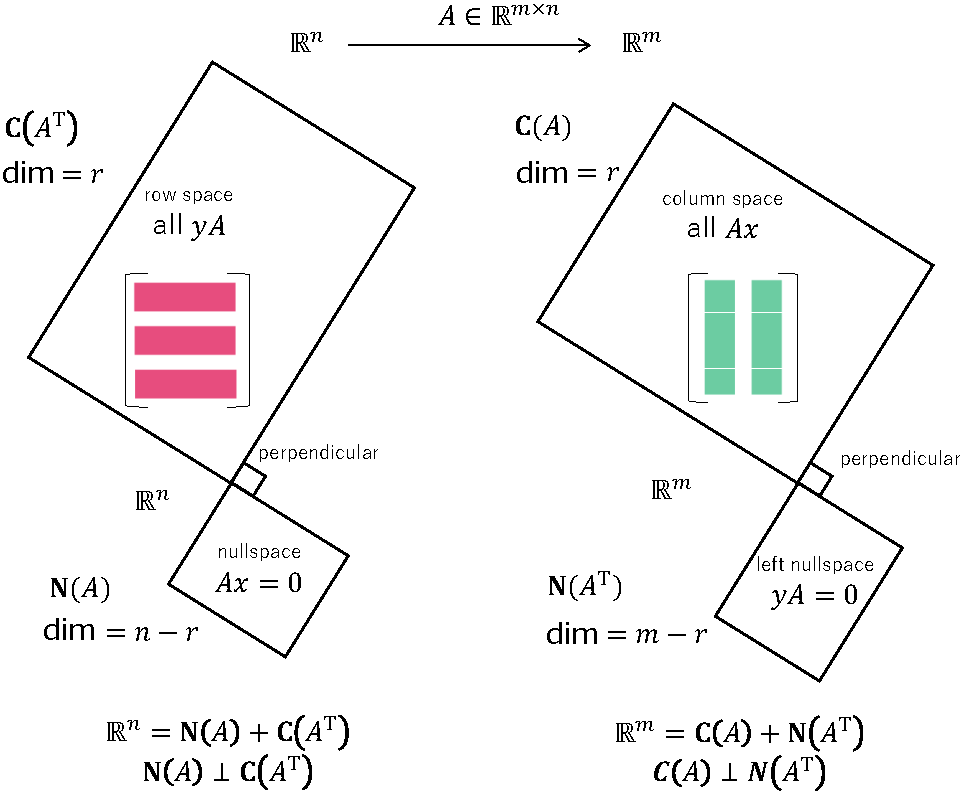
\includegraphics[width=13cm,height=10cm]{"figure/Question/四个子空间.pdf"}
	\caption{四个子空间}
\end{figure} 
\begin{solution}

	(1). 我们可以知道矩阵$A$的零空间为$N(A)=R^{n}$,我们可以得到$A$的行空间$R(A)=0$,$A=0$
	
	(2). 当$A$为反对称矩阵时,我们可以得到$\xi^{T}A\xi=0$
	
	(3). 我们不妨取$B=E$,可以得到$A=0$,矩阵$A$只能为零矩阵,在$A=0$时,任意的$n$阶矩阵$B$满足$AB=0$
	
	(4). 同$(3)$,取$B=E$,可以得到$A=0$,矩阵$A$只能为零矩阵,在$A=0$时,任意的$n$阶矩阵$B$满足$B^{T}AB=0$
\end{solution}
\myspace{1}

2. 设函数$f(x)$在$(\dfrac{1}{2},+\infty)$上可导,且$\lim\limits_{h\to 0}\dfrac{f[(x+h)^2]-f(x^2+h)}{h}=1$,$f(1)=1$,求$f(x)$
\myspace{1}
\begin{solution}

	原极限等价于:  
	\begin{eqnarray*}
		I&=&\lim\limits_{h\to 0}\dfrac{f[(x+h)^2]-f(x^2+h)}{h}\\
		&=&\lim\limits_{h\to 0}\dfrac{f[(x+h)^2]-f(x^2)+f(x^2)-f(x^2+h)}{h}\\
		&=&\lim\limits_{h\to 0}\dfrac{f[(x+h)^2]-f(x^2)}{h}+\lim\limits_{h\to 0}\dfrac{f(x^2)-f(x^2+h)}{h}\\
		&=&[f(x^2)]'-f'(x^2)\\
		&=&(2x-1)f'(x^2)\\
		&=&1
	\end{eqnarray*}

	我们得到:  
	$$f'(x^2)=\dfrac{1}{2x-1}\Rightarrow 2xf'(x^2)=\dfrac{2x}{2x-1}\Rightarrow f(x^2)=x+\dfrac{1}{2}\ln(2x-1)+C$$
	
	我们由$f(1)=1\Rightarrow C=0\Rightarrow f(x^2)=x+\dfrac{1}{2}\ln(2x-1)$
	
	我们得到$f(x)=\sqrt{x}+\dfrac{1}{2}\ln(2\sqrt{x}-1)$
\end{solution}
\myspace{1}

\textcolor{blue}{August 9}

1. $f(x)$在$[0,1]$上导函数连续,$f(0)=f(1)=0$,证明:  $\int_{0}^{1}f^{2}(x)dx\leq \dfrac{1}{8}\int_{0}^{1}[f'(x)]^2dx$
\myspace{1}
\begin{theorem}[积分形式柯西不等式]
	$$\left[ \int_{a}^{b}f(x)g(x)dx\right] ^2\leq \int_{a}^{b}f^2(x)dx\int_{a}^{b}g^{2}(x)dx$$
	
	我们知道$\forall t\in\mathbb{R}$,我们有:  
	$$\left[ tf(x)-g(x)\right]^2\geq 0\Rightarrow t^2f^{2}(x)-2tf(x)g(x)+g^{2}(x)\geq 0$$
	
	我们对上式子两边在区间$[a,b]$上积分,可以得到:  
	$$t^2\int_{a}^{b}f^{2}(x)dx-2t\int_{a}^{b}f(x)g(x)dx+\int_{a}^{b}g^{2}(x)dx\geq 0$$
	
	我们可以得到一个关于$t$的一元二次方程方程:  
	$$At^2+Bt+C\geq 0,\text{其中}\left\lbrace
	\begin{array}{l}
		A=\int_{a}^{b}f^{2}(x)dx\\
		B=-2\int_{a}^{b}f(x)g(x)dx\\
		C=\int_{a}^{b}g^{2}(x)dx
	\end{array}
	\right. \Rightarrow B^2-4AC\leq 0$$
	
	我们得到:  $$4\left[ \int_{a}^{b}f(x)g(x)dx\right]^2-4\int_{a}^{b}f^{2}(x)dx\int_{a}^{b}g^{2}(x)dx\leq 0 
	$$
	$$\left[ \int_{a}^{b}f(x)g(x)dx\right] ^2\leq \int_{a}^{b}f^2(x)dx\int_{a}^{b}g^{2}(x)dx$$
\end{theorem}
\begin{solution}

	我们知道:  $\left\lbrace
	\begin{array}{l}
		f(x)=\int_{0}^{x}f'(t)dt\\
		f(x)=\int_{1}^{x}f'(t)dt
	\end{array}
	\right. $
	我们有:  $$\int_{0}^{1}f^{2}(x)dx=\left\lbrace
	\begin{array}{l}
		\int_{0}^{1}\left[\int_{0}^{x}f'(t)dt \right]^2dx\leq \int_{0}^{1}[\int_{0}^{x}1^2dt\int_{0}^{x}|f'(t)|^2dt]dx\\
		\int_{0}^{1}\left[\int_{1}^{x}f'(t)dt \right]^2dx\leq \int_{0}^{1}[\int_{1}^{x}1^2dt\int_{0}^{x}|f'(t)|^2dt]dx
	\end{array}
	\right.$$
	
	我们可以得到:  
	\begin{eqnarray*}
		\int_{0}^{1}f^{2}(x)dx&=&\int_{0}^{\frac{1}{2}}f^{2}(x)dx+\int_{\frac{1}{2}}^{1}f^{2}(x)dx\\
		&=&\int_{0}^{\frac{1}{2}}\left[\int_{0}^{x}f'(t)dt \right]^2dx+\int_{\frac{1}{2}}^{1}\left[\int_{x}^{1}f'(t)dt \right]^2dx\\
		&\leq&\int_{0}^{\frac{1}{2}}[\int_{0}^{x}1^2dt\int_{0}^{x}|f'(t)|^2dt]dx+\int_{\frac{1}{2}}^{1}[\int_{x}^{1}1^2dt\int_{x}^{1}|f'(t)|^2dt]dx\\
		&\leq&\int_{0}^{\frac{1}{2}}[x\int_{0}^{x}|f'(t)|^2dt]dx+\int_{\frac{1}{2}}^{1}[(1-x)\int_{x}^{1}|f'(t)|^2dt]dx\\
		&=&\int_{0}^{\frac{1}{2}}|f'(t)|^2dt\int_{t}^{\frac{1}{2}}xdx+\int_{\frac{1}{2}}^{1}|f'(t)|^2dt\int_{\frac{1}{2}}^{t}(1-x)dx\\
		&=&(\dfrac{1}{8}-\dfrac{t^2}{2})\int_{0}^{\frac{1}{2}}|f'(t)|^2dt+(t-\dfrac{t^2}{2}-\dfrac{3}{8})\int_{\frac{1}{2}}^{1}|f'(t)|^2dt\\
		&=&\dfrac{1}{8}\int_{0}^{\frac{1}{2}}|f'(t)|^2dt+\dfrac{1}{8}\int_{\frac{1}{2}}^{1}|f'(t)|^2dt\\
		&=&\dfrac{1}{8}\int_{0}^{1}[f'(x)]^2dx
	\end{eqnarray*}
\end{solution}
\myspace{1}

2. 求$\lim\limits_{n\to+\infty}\left[\sqrt{n}(\sqrt{n+1}-\sqrt{n})+\dfrac{1}{2} \right]^{\dfrac{\sqrt{n+1}+\sqrt{n}}{\sqrt{n+1}-\sqrt{n}}} $
\myspace{1}
\begin{solution}

	原极限等价于:  
	\begin{eqnarray*}
		I&=&e^{\lim\limits_{n\to+\infty}\dfrac{\ln\left( 1+\dfrac{\sqrt{n}-\sqrt{n+1}}{2(\sqrt{n+1}+\sqrt{n})}\right)}{(\sqrt{n+1}-\sqrt{n})^2}}\\
		&=&e^{\lim\limits_{n\to+\infty}\dfrac{\dfrac{\sqrt{n}-\sqrt{n+1}}{2(\sqrt{n+1}+\sqrt{n})}}{(\sqrt{n+1}-\sqrt{n})^2}}\\
		&=&e^{\lim\limits_{n\to+\infty}-\dfrac{1}{2}}\\
		&=&e^{-\frac{1}{2}}
	\end{eqnarray*}
\end{solution}
\myspace{1}

\textcolor{blue}{August 10}

1. 设可导函数$y=y(x)$由方程$\sin x-\int_{x}^{y}\varphi(u)du=0$所确定,其中可导函数$\varphi(u)>0$,且$\varphi(0)=\varphi'(0)=1$,求$y''(0)$
\myspace{1}
\begin{solution}

	我们可以得到:  当$x=0$时,$\int_{0}^{y}\varphi(u)du=0$,且$\varphi(u)>0$,我们得到$y=0$.
	
	我们对方程$\sin x-\int_{x}^{y}\varphi(u)du=0$两边对$x$求导得到:  
	$$\left\lbrace
	\begin{array}{l}
		\cos x-[\varphi(y)y'-\varphi(x)]=0\\
		-\sin x-[\varphi'(y)y'^2+\varphi(y)y''-\varphi'(x)]=0
	\end{array}
	\right. \Rightarrow \left\lbrace
	\begin{array}{l}
		1-y'(0)\varphi(0)+\varphi(x)=0\\
		-\varphi'(0)y'(0)^2-y''(0)\varphi(0)+\varphi'(0)=0
	\end{array}
	\right. \Rightarrow \left\lbrace
	\begin{array}{l}
		y'(0)=2\\
		y''(0)=-3
	\end{array}
	\right. $$
\end{solution}
\myspace{1}

2. 设$a_{n}=\int_{0}^{1}\dfrac{x^n}{1+x}dx$

(1).证明:  $\dfrac{1}{2(n+1)}\leq a_{n}\leq \dfrac{1}{2n},\ n=1,2,\cdots$

(2). 证明:  级数$\sum\limits_{n=1}^{+\infty}(-1)^{n-1}(\dfrac{1}{2n}-\int_{0}^{1}\dfrac{x^n}{1+x}dx)$绝对收敛.
\myspace{1}
\begin{solution}

	(1). 我们有:  $$\left\lbrace
	\begin{array}{l}
		\dfrac{x^n}{1+x}\geq \dfrac{x^n}{2},\ x\in(0,1)\\
		\dfrac{x^n}{1+x}=\dfrac{x}{1+x}x^{n-1}\leq\dfrac{x^{n-1}}{2},\ x\in(0,1)
	\end{array}
	\right. \Rightarrow \int_{0}^{1}\dfrac{x^n}{2}dx\leq \int_{0}^{1}\dfrac{x^n}{1+x}dx\leq \int_{0}^{1}\dfrac{x^{n-1}}{2}dx$$
	
	我们有:  $$\left\lbrace
	\begin{array}{l}
		\int_{0}^{1}\dfrac{x^n}{2}dx=\dfrac{x^{n+1}}{2(n+1)}|_{0}^{1}=\dfrac{1}{2(n+1)}\\
		\int_{0}^{1}\dfrac{x^{n-1}}{2}dx=\dfrac{x^{n}}{2n}|_{0}^{1}=\dfrac{1}{2n}
	\end{array}
	\right. $$
	
	我们证明了:  $\dfrac{1}{2(n+1)}\leq a_{n}\leq \dfrac{1}{2n},\ n=1,2,\cdots$
	
	(2). 我们不妨设$b_{n}=\dfrac{1}{2n}-a_{n}=\dfrac{1}{2n}-\int_{0}^{1}\dfrac{x^n}{1+x}dx$.
	
	我们由$(1)$可得:  $|b_{n}|\leq \dfrac{1}{2n}-\dfrac{1}{2(n+2)}=\dfrac{1}{2n^2+4n}<\dfrac{1}{2n^2}$
	
	我们知道级数$\sum\limits_{n=1}^{+\infty}\dfrac{1}{2n^2}$收敛,由比较判别法我们可知级数$\sum\limits_{n=1}^{+\infty}b_{n}$收敛,原级数绝对收敛.
\end{solution}
\myspace{1}

\textcolor{blue}{August 11}

1. 设$x=x(y)$是函数$y=\ln x+e^x$的反函数,求$\dfrac{d^2x}{dy^2}$.
\myspace{1}
\begin{solution}

	我们有:  $\left\lbrace
	\begin{array}{l}
		y=f(x)\\
		x=g(y)
	\end{array}
	\right. \Rightarrow \left\lbrace
	\begin{array}{l}
		y'(x)=f'(x)\\
		1=f'(x)g'(y)
	\end{array}
	\right. \Rightarrow g'(y)=\dfrac{1}{f(x)}$
	
	我们有:  $f(x)=\ln x+e^x\Rightarrow f'(x)=e^x+\dfrac{1}{x}$
	
	我们得到:  $g'(y)=\dfrac{dx}{dy}=\dfrac{1}{f(x)}=\dfrac{x}{1+xe^x}$
	
	我们有:  
	$$\dfrac{d^2x}{dy^2}=\dfrac{\dfrac{dx}{dy}}{dx}\dfrac{dx}{dy}=\dfrac{x-x^3e^x}{(1+xe^x)^3}$$
\end{solution}
\myspace{1}

2. 设$a_{0}=1,a_{1}=0$,$a_{n+1}=\dfrac{1}{n+1}(na_{n}+a_{n-1})\ (n=1,2,3\cdots)$,$S(x)$为幂级数$\sum\limits_{n=0}^{+\infty}a_{n}x^{n}$的和函数.

(1).证明:  幂级数$\sum\limits_{n=0}^{+\infty}a_{n}x^n$的收敛半径不小于$1$.

(2).证明:  $(1-x)S'(x)-xS(x)=0,\ x\in(-1,1)$,并求出$S(x)$的表达式.
\myspace{1}
\begin{solution}

	(1). 我们由$a_{n+1}=\dfrac{1}{n+1}(na_{n}+a_{n-1})$得到:  
	$$a_{n+1}-a_{n}=-\dfrac{1}{n+1}(a_{n}-a_{n-1})$$
	
	我们不妨设$b_{n}=a_{n}-a_{n-1}\Rightarrow b_{n+1}=-\dfrac{1}{n+1}b_{n},\ b_{1}=a_{1}-a_{0}=-1$
	
	我们有:  $$\left\lbrace
	\begin{array}{l}
		b_{n}=-\dfrac{1}{n}b_{n-1}\\
		b_{n-1}=-\dfrac{1}{n-1}b_{n-2}\\
		\cdots\\
		b_{2}=-\dfrac{1}{2}b_{1}\\
		b_{1}=-1
	\end{array}
	\right. \Rightarrow b_{n}=\dfrac{(-1)^{n}}{n!}$$
	
	我们由累加法可以得到:  $a_{n}=\left\lbrace
	\begin{array}{l}
		a_{0}+\sum\limits_{k=1}^{n}b_{k}=\sum\limits_{k=0}^{n}\dfrac{(-1)^k}{k!},\ n\geq 1\\
		1,\ n=0
	\end{array}
	\right. \Rightarrow a_{n}=\sum\limits_{k=0}^{n}\dfrac{(-1)^k}{k!}$
	
	我们利用根值审敛法:  
	$$\rho=\lim\limits_{n\to+\infty}\sqrt[n]{a_{n}}=e^{\lim\limits_{n\to +\infty}\dfrac{\ln(\sum\limits_{k=0}^{n}\dfrac{(-1)^k}{k!})}{n}}=1$$
		
	我们得到级数的收敛半径:  $r=\dfrac{1}{\rho}=1$,幂级数$\sum\limits_{n=0}^{+\infty}a_{n}x^n$的收敛半径不小于$1$.

	(2). 我们有:  $S(x)=\sum\limits_{n=0}^{+\infty}a_{n}x^{n}$,我们得到:  
	$$\left\lbrace
	\begin{array}{l}
		S'(x)=\sum\limits_{n=1}^{+\infty}na_{n}x^{n-1}=\sum\limits_{n=0}^{+\infty}(n+1)a_{n+1}x^{n}\\
		S(x)=\sum\limits_{n=0}^{+\infty}a_{n}x^{n}
	\end{array}
	\right.$$
	
	$$a_{n+1}=\dfrac{1}{n+1}(na_{n}+a_{n-1})\Rightarrow (n+1)a_{n+1}=na_{n}+a_{n-1}\Rightarrow (n+2)a_{n+2}=(n+1)a_{n+1}=a_{n}$$
	
	我们得到:  
	\begin{eqnarray*}
		(1-x)S'(x)-xS(x)&=&(1-x)\sum\limits_{n=0}^{+\infty}(n+1)a_{n+1}x^{n}-x\sum\limits_{n=0}^{+\infty}a_{n}x^{n}\\
		&=&\sum\limits_{n=0}^{+\infty}(n+1)a_{n+1}x^{n}-\sum\limits_{n=0}^{+\infty}[(n+1)a_{n+1}+a_{n}]x^{n+1}\\
		&=&a_{1}+\sum\limits_{n=1}^{+\infty}(n+1)a_{n+1}x^{n}-\sum\limits_{n=0}^{+\infty}[(n+1)a_{n+1}+a_{n}]x^{n+1}\\
		&=&\sum\limits_{n=0}^{+\infty}(n+2)a_{n+2}x^{n+1}-\sum\limits_{n=0}^{+\infty}[(n+1)a_{n+1}+a_{n}]x^{n+1}\\
		&=&\sum\limits_{n=0}^{+\infty}[(n+2)a_{n+2}-(n+1)a_{n+1}-a_{n}]x^{n+1}\\
		&=&0
	\end{eqnarray*}
	
	我们得到:  
	$$(1-x)S'(x)-xS(x)=0\Rightarrow \dfrac{S'(x)}{S(x)}=\dfrac{x}{1-x}\Rightarrow S(x)=\dfrac{C_{1}}{e^x(1-x)}$$
	
	我们有$S(0)=1\Rightarrow C_{1}=1$,因此$S(x)=\dfrac{1}{e^x(1-x)},\ x\in(-1,1)$
	
\end{solution}
\myspace{1}

\textcolor{blue}{August 12}

1. 设$y=y(x)$由$e^y\sin t-y+1=0$和$x=\left\lbrace
\begin{array}{l}
	\dfrac{e^t-1}{t},\ t\neq 0\\
	1,\ t=0
\end{array}
\right. $所确定,求$\dfrac{d^2y}{dx^2}|_{t=0}$
\myspace{1}
\begin{solution}

	我们知道:  当$t=0$时,$\left\lbrace
	\begin{array}{l}
		x=1\\y=1
	\end{array}
	\right. $,我们由:  
	$$x(t)=\left\lbrace
	\begin{array}{l}
		\dfrac{e^t-1}{t},\ t\neq 0\\
		1,\ t=0
	\end{array}
	\right. \Rightarrow x(t)=1+\dfrac{t}{2}+\dfrac{t^2}{6}+\dfrac{t^3}{24}+\cdots\Rightarrow \left\lbrace
	\begin{array}{l}
		x'(0)=\dfrac{1}{2}\\
		x''(0)=\dfrac{1}{3}
	\end{array}
	\right. $$
	
	我们由:  $e^y\sin t-y+1=0\Rightarrow e^{y(t)}\sin t-y(t)+1=0$得到:  
	$$\left\lbrace
	\begin{array}{l}
		e^{y(t)}\cos t+y'(t)e^{y(t)}\sin t-y'(t)=0\\
		y'(t)e^{y(t)}\cos t-e^{y(t)}\sin t+\left\lbrace [y'(t)]^2e^{y(t)}+y''(t)e^{y(t)}\right\rbrace \sin x+\cos x\left[y'(t)e^{y(t)} \right]-y''(t)=0
	\end{array}
	\right.$$
	$$\left\lbrace
	\begin{array}{l}
		y'(0)=e\\
		y''(0)=2e^2
	\end{array}
	\right. $$
	
	我们由参数方程二阶导数公式:  
	$$\dfrac{d^2y}{dx^2}|_{t=0}=\dfrac{y''(t)x'(t)-x''(t)y'(t)}{[x'(t)]^3}|_{t=0}=8e^2-\dfrac{8e}{3}$$
	
\end{solution}
\myspace{1}

2. 下列命题正确的是:  
\begin{itemize}
	\item \hl{A}. 设$A$为$3$阶矩阵,若$A$的特征值$\lambda_{1}\lambda_{2}\neq 0,\lambda_{3}=0$,则$r(A)=2$
	\item \hl{B}. 设$A$为$3$阶非零矩阵,若$A^2=0$,则$r(A)=1$
	\item C. 设$A,B$为$3$阶矩阵,若$A$与$B$等价,则$|A|=|B|$
	\item D. 设$A,B$为$3$阶实对称矩阵,若$A$与$B$合同,则$|A|=|B|$
\end{itemize}
\myspace{1}
\begin{solution}

	(A). 我们可以得到矩阵$A\sim diag\{\lambda_{1},\lambda_{2},\lambda_{3}\}$,对角矩阵的秩和矩阵$A$的秩相同,$r(A)=2$
	
	(B). $A^2=0\Rightarrow 2r(A)\leq 3\Rightarrow r(A)=1$
	
	(C). $A$与$B$等价$\Rightarrow r(A)=r(B)$
	
	(D). $A$与$B$合同$\Rightarrow A=P^{T}BP$
\end{solution}
\myspace{1}

\textcolor{blue}{August 13}

1. 已知$f(x)=\left\lbrace
\begin{array}{l}
	\lim\limits_{n\to +\infty}\left( 1+\dfrac{2nx+x^2}{2n^2}\right)^{-n},\ x\neq 0\\
	\lim\limits_{n\to +\infty}2\left[ \dfrac{n}{(n+1)^2}+\dfrac{n}{(n+2)^2}+\cdots+\dfrac{n}{(n+n)^2}\right],\ x=0  
\end{array}
\right. $,求$\int f(x)dx$
\myspace{1}
\begin{solution}

	当$x\neq 0$时:  
	\begin{eqnarray*}
		f(x)&=&\lim\limits_{n\to +\infty}\left( 1+\dfrac{2nx+x^2}{2n^2}\right)^{-n}\\
		&=&e^{\lim\limits_{n\to +\infty}(-n)\dfrac{2nx+x^2}{2n^2}}\\
		&=&e^{-x}
	\end{eqnarray*}

	当$x=0$时:  
	\begin{eqnarray*}
		f(x)&=&\lim\limits_{n\to +\infty}2\left[ \dfrac{n}{(n+1)^2}+\dfrac{n}{(n+2)^2}+\cdots+\dfrac{n}{(n+n)^2}\right]\\
		&=&2\lim\limits_{n\to +\infty}\dfrac{1}{n}\left[ \dfrac{1}{(1+\dfrac{1}{n})^2}+\dfrac{1}{(1+\dfrac{2}{n})^2}+\cdots+\dfrac{1}{(1+\dfrac{n}{n})^2}\right]\\
		&=&2\int_{0}^{1}\dfrac{1}{(1+x)^2}dx\\
		&=&2(1-\dfrac{1}{2})\\
		&=&1
	\end{eqnarray*}

	我们得到:  $f(x)=e^{-x}\Rightarrow \int f(x)dx=-e^{-x}+C$
\end{solution}
\myspace{1}

2. 已知函数$f(x)=x^2\ln(1-x)$,当$n\geq 3$时,求$f^{(n)}(0)$
\myspace{1}
\begin{solution}

	我们利用$\ln(1-x)$的泰勒展开式:  
	$$\ln(1-x)=-x-\dfrac{x^2}{2}-\dfrac{x^3}{3}-\cdots-\dfrac{x^n}{n}-\cdots$$
	
	我们可以得到:  
	$$f(x)=-x^3-\dfrac{x^4}{2}-\dfrac{x^5}{3}-\cdots-\dfrac{x^n+2}{n}-\cdots$$
	
	我们有:  
	$$\left\lbrace
	\begin{array}{l}
		f'(0)=0\\
		f''(0)=0\\
		f^{(3)}(0)=-6\\
		f^{(4)}(0)=-\dfrac{4!}{2}\\
		\cdots\cdots
	\end{array}
	\right. \Rightarrow f^{(n)}(0)=-\dfrac{n!}{n-2},\ n\geq 3$$
\end{solution}
\myspace{1}

\textcolor{blue}{August 14}

1. 设$f(x)$在$[0,1]$上可导,$f(0)=f(1)=-2$,证明:  $\exists \xi\in(0,1),\ s.t. f'(\xi)-f(\xi)=\xi$
\myspace{1}
\begin{solution}

	我们构造辅助函数:  $F(x)=e^{-x}\left[ f(x)+x+1\right]$,我们有:  
	$$F(0)=-1,\ F(1)=0,\ F'(x)=e^{-x}\left[ f'(x)-f(x)-x\right]$$
	
	我们由积分中值定理可以得到:  
	$$\exists \eta\in(0,1),\ s.t. \int_{0}^{1}f(x)dx=f(\eta)\Rightarrow \exists \eta\in(0,1),\ s.t. f(\eta)=0$$
	
	我们有:  
	$$F(\eta)=e^{-\eta}\left[ f(\eta)+\eta+1\right]=e^{-\eta}(\eta+1)>0$$
	
	我们根据零点定理,可知:  $\exists \delta\in(0,\eta),\ s.t. F(\delta)=0$.
	
	我们对$F(x)$在区间$[\delta,1]$上使用罗尔定理可以得到:  
	$$\exists\xi\in(\delta,1),\ s.t. F'(\xi)=e^{-\xi}\left[ f'(\xi)-f(\xi)-\xi\right]=0\Rightarrow f'(\xi)-f(\xi)=\xi$$
	
	综上所述,我们得到:  $\exists \xi\in(0,1),\ s.t. f'(\xi)-f(\xi)=\xi$
\end{solution}
\myspace{1}

2. 设数列$\{u_{n}\}$满足$u_{1}=1,\ u_{n+1}=\dfrac{u_{n}+3}{u_{n}+1},\ (n=1,2,\cdots)$,试证明数列$\{u_{n}\}$收敛,并求其极限.
\myspace{1}
\begin{solution}

	我们有:
	$$u_{1}=1,\ u_{2}=2,\ u_{3}=\dfrac{5}{3},\ u_{4}=\dfrac{7}{4},\cdots\ (u_{n}>0)$$
	
	我们发现数列$\{u_{n}\}$不是单调数列,我们从奇数项和偶数项入手:
	$$\left\lbrace
	\begin{array}{l}
		u_{2k+2}=\dfrac{u_{2k+1}+3}{u_{2k+1}+1}=\dfrac{\frac{u_{2k}+3}{u_{2k}+1}+3}{\frac{u_{2k}+3}{u_{2k}+1}+1}=2-\dfrac{1}{u_{2k}+2}\\
		u_{2k+1}=\dfrac{u_{2k}+3}{u_{2k}+1}=\dfrac{\frac{u_{2k-1}+3}{u_{2k-1}+1}+3}{\frac{u_{2k-1}+3}{u_{2k-1}+1}+1}=2-\dfrac{1}{u_{2k-1}+2}
	\end{array}
	\right. \Rightarrow f(x)=2-\dfrac{1}{x+2}\text{单调递增}$$
	
	我们首先证明数列$\{u_{2k-1}\}$极限存在:  
	
	(1). 当$n=1$时,$u_{1}<u_{3}$.
	
	(2). 当$n=k$时,假设$u_{2k-1}<u_{2k+1}$
	
	(3). 当$n=k+1$时,$u_{2k-1}<u_{2k+1}\Rightarrow f(u_{2k-1})<f(u_{2k+1})\Rightarrow u_{2k+1}<u_{2k+3}$
	
	数列$\{u_{2k-1}\},(k=1,2,\cdots)$单调递增,且$u_{2k-1}<2$
	
	我们继续证明数列$\{u_{2k}\}$极限存在:  
	
	(1). 当$n=1$时,$u_{2}>u_{4}$.
	
	(2). 当$n=k$时,假设$u_{2k}>u_{2k+2}$
	
	(3). 当$n=k+1$时,$u_{2k}>u_{2k+2}\Rightarrow f(u_{2k})>f(u_{2k+2})\Rightarrow u_{2k+2}<u_{2k+4}$
	
	数列$\{u_{2k}\},(k=1,2,\cdots)$单调递减少,且$u_{2k}>\dfrac{3}{2}$
	
	我们不妨假设:  $$\left\lbrace
	\begin{array}{l}
		\lim\limits_{k\to +\infty}u_{2k-1}=A\\
		\lim\limits_{k\to +\infty}u_{2k}=B\\
	\end{array}
	\right. \Rightarrow \left\lbrace
	\begin{array}{l}
		A=\dfrac{B+3}{B+1}\\
		B=\dfrac{A+3}{A+1}
	\end{array}
	\right. \Rightarrow A=B=\sqrt{3}$$
	
	我们可以得到:  
	
	(1). $\forall \varepsilon>0$,$\exists N_{1}>0$,当$n=2k-1>N_{1}$时,我们有:$|u_{2k-1}-\sqrt{3}|<\varepsilon$.
	
	(2). $\forall \varepsilon>0$,$\exists N_{2}>0$,当$n=2k>N_{2}$时,我们有:$|u_{2k}-\sqrt{3}|<\varepsilon$.
	
	(3). 取$N=\text{max}\{N_{1},N_{2}\}$,$\forall \varepsilon>0$,$\exists N>0$,当$n>N$时,我们有:$|u_{n}-\sqrt{3}|<\varepsilon$.
	
	综上所述,我们证明数列$\{u_{n}\}$收敛,极限为$\sqrt{3}$.
\end{solution}
\myspace{1}

\section{Week \Rmnum{3}}
\textcolor{cyan}{August 15}

1. $f(x)=\int_{1}^{x}\dfrac{\arctan t}{(1+t^2)^{\frac{3}{2}}\ln(1+t^2)}dt$,求$\int_{0}^{1}\dfrac{x}{1+x^2}f(x)dx$
\myspace{1}
\begin{solution}

	原定积分等价于:  
	\begin{eqnarray*}
		I&=&\int_{0}^{1}\dfrac{f(x)}{2}d(\ln(1+x^2))\\
		&=&\dfrac{f(x)\ln(1+x^2)}{2}|_{x=0}^{x=1}-\int_{0}^{1}\dfrac{\ln(1+x^2)}{2}d(f(x))\\
		&=&-\int_{0}^{1}\dfrac{\arctan x}{2(1+x^2)^{\frac{3}{2}}}dx\\
		&=&-\dfrac{1}{2}\int_{0}^{\frac{\pi}{4}}\theta\cos\theta d\theta\\
		&=&-\dfrac{1}{2}\theta\sin\theta|_{\theta=0}^{\theta=\frac{\pi}{4}}-\dfrac{1}{2}\int_{0}^{\frac{\pi}{4}}\sin \theta d\theta\\
		&=&-\dfrac{\sqrt{2}\pi}{16}+\dfrac{2-\sqrt{2}}{4}
	\end{eqnarray*}
\end{solution}
\myspace{1}

2. 设$f(x)=\dfrac{1}{1+2x+4x^2}$,求$f^{(100)}(0)$
\myspace{1}
\begin{solution}

	$$f(x)=\dfrac{1-2x}{(1-2x)(4x^2+2x+1)}=\dfrac{1-2x}{1-(2x)^3}$$
	$$\dfrac{1}{1-(2x)^3}=1+(2x)^3+(2x)^6+(2x)^9+\cdots+(2x)^{3n}$$
	
	我们得到:$$f(x)=(1-2x)\sum\limits_{n=0}^{+\infty}(2x)^{3n}=\sum\limits_{n=0}^{+\infty}(2x)^{3n}-\sum\limits_{n=0}^{+\infty}(2x)^{3n+1}$$
	$$f(x)=f(0)+f'(0)x+\cdots+\dfrac{f^{(n)}(0)}{n!}x^n$$
	
	$\dfrac{f^{(100)}(0)}{100!}$是$f(x)$中$x^{100}$前面的系数,我们可以得到:  
	$$f^{(100)}(0)=-2^{100}\times100!$$
\end{solution}
\myspace{1}

\textcolor{cyan}{August 16}

1. 证明:  在区间$(0,2)$内存在三个不同的点$x_{1},x_{2},x_{3}$,使得$\dfrac{1-\ln(1+x_{1})}{(1+x_{1})^2}x_{3}=\dfrac{1-\ln(1+x_{2})}{(1+x_{2})^2}(2-x_{3})$
\myspace{1}
\begin{solution}

	我们构造辅助函数:  $f(x)=\dfrac{\ln(1+x)}{1+x}$,我们有:  
	$$\left\lbrace 
	\begin{array}{l}
		f'(x)=\dfrac{1-\ln(1+x)}{(1+x)^2}\\
		f(0)=0\\
		f(2)=\dfrac{\ln 3}{3}
	\end{array}
	\right. $$
	
	我们不妨假设$\exists x_{3}\in(0,2), f(x_{3})=A$,我们分别在区间$(0,x_{3})$和区间$(x_{3},2)$上使用拉格朗日中值定理可以得到:  
	$$\left\lbrace 
	\begin{array}{l}
		\exists x_{1}\in(0,x_{3}),\ s.t. \dfrac{f(x_{3})-f(0)}{x_{3}}=f'(x_{1})=\dfrac{1-\ln(1+x_{1})}{(1+x_{1})^2}\\
		\exists x_{2}\in(x_{3},2),\ s.t. \dfrac{f(2)-f(x_{3})}{2-x_{3}}=f'(x_{2})=\dfrac{1-\ln(1+x_{2})}{(1+x_{2})^2}
	\end{array}
	\right. $$
	
	我们令$f(x_{3})-f(0)=f(2)-f(x_{3})\Rightarrow A=f(2)-A\Rightarrow f(x_{3})=A=\dfrac{f(2)}{2}=\dfrac{\ln 3}{6}$时,我们可以得到:  $$\dfrac{1-\ln(1+x_{1})}{(1+x_{1})^2}x_{3}=\dfrac{1-\ln(1+x_{2})}{(1+x_{2})^2}(2-x_{3})$$
	
	综上所述,我们可以得到:  在区间$(0,2)$内存在三个不同的点$x_{1},x_{2},x_{3}$,使得$\dfrac{1-\ln(1+x_{1})}{(1+x_{1})^2}x_{3}=\dfrac{1-\ln(1+x_{2})}{(1+x_{2})^2}(2-x_{3})$
\end{solution}
\myspace{1}

2. 设$y=\dfrac{\arcsin x}{\sqrt{1-x^2}}$

(1). 证明:  $(1-x^2)y^{(n+1)}-(2n+1)xy^{(n)}-n^2y^{(n-1)}=0(n\geq 1)$;

(2). 求$y^{(n)}(0)$
\myspace{1}
\begin{solution}

	(1). 我们对$f(x)$求导可以得到:  
	$$f'(x)=\dfrac{1+\dfrac{x\arcsin x}{\sqrt{1-x^2}}}{1-x^2}\Rightarrow f'(x)=\dfrac{1+xf(x)}{1-x^2}\Rightarrow (1-x^2)f'(x)-xf(x)-1=0$$
	
	我们令$g(x)=(1-x^2)f'(x)-xf(x)-1$,我们利用莱布尼兹公式可以得到:  
	$$g^{(n)}(x)=\sum\limits_{k=0}^{n}C_{n}^{k}(1-x^2)^{(k)}f^{(n-k+1)}(x)-\sum\limits_{k=0}^{n}C_{n}^{k}(x)^{(k)}f^{(n-k)}=0$$
	
	当$k\geq 3$时,$(1-x^2)^{(k)}=0$;当$k\geq 2$时,$x^{(k)}=0$,我们有:  
	$$g^{(n)}(x)=(1-x^2)f^{(n+1)}(x)-2nxf^{(n)}(x)-n(n-1)f^{(n-1)}(x)-xf^{(n)}(x)-nf^{(n-1)}(x)=0$$
	
	我们得到:  
	$$(1-x^2)f^{(n+1)}(x)-(2n+1)xf^{(n)}(x)-n^2f^{(n-1)}(x)=0$$
	
	综上所述,我们得到:  $(1-x^2)y^{(n+1)}-(2n+1)xy^{(n)}-n^2y^{(n-1)}=0(n\geq 1)$
	
	(2). 我们将$x=0$代入上面式子可以得到:  
	$$\left\lbrace 
	\begin{array}{l}
		y^{(n)}=(n-1)^2y^{(n-2)}\\
		y(0)=0\\
		y^{(1)}(0)=1
	\end{array}
	\right. \Rightarrow y^{(n)}(0)=\left\lbrace 
	\begin{array}{l}
		0,\ n\text{为偶数},n=2k(k=0,1,\cdots)\\
		(2k!!)^2,\ n\text{为奇数},n=2k+1(k=0,1,\cdots)
	\end{array}
	\right. $$
\end{solution}
\myspace{1}

\textcolor{cyan}{August 17}

1. 已知极限$\lim\limits_{t\to x}\left(\dfrac{\sin t}{\sin x} \right)^{\dfrac{x}{\sin t-\sin x}}$,记此极限为$f(x)$,求函数$f(x)$的间断点,并指出其类型.
\myspace{1}
\begin{solution}

	$$f(x)=e^{\lim\limits_{t\to x}\frac{x}{\sin t-\sin x}\ln(1+\frac{\sin t-\sin x}{\sin x})}=e^{\frac{x}{\sin x}}$$
	
	我们发现$f(x)$的间断点为$x=k\pi,\ k\in\mathbb{Z}$.
	
	(1). 当$k=0$时,我们有:
	$$\left\lbrace 
	\begin{array}{l}
		\lim\limits_{x\to 0^{+}}f(x)=e\\
		\lim\limits_{x\to 0^{-}}f(x)=e
	\end{array}
	\right. \Rightarrow x=0\text{是}f(x)\text{可去间断点}$$
	
	(2). 当$k\neq 0$时,我们有:
	$$\left\lbrace 
	\begin{array}{l}
		\lim\limits_{x\to k\pi^{+}}f(x)=+\infty\text{或者}0\\
		\lim\limits_{x\to 0^{-}}f(x)=0\text{或者}+\infty
	\end{array}
	\right. \Rightarrow x=k\pi\text{是}f(x)\text{无穷间断点}$$
\end{solution}
\myspace{1}

2. 证明:  $\int_{0}^{\pi}xa^{\sin x}dx\int_{0}^{\frac{\pi}{2}}a^{-\cos x}dx\geq \dfrac{\pi^3}{4}$
\myspace{1}
\begin{solution}

	我们由区间再现公式可以得到:
	$$\left\lbrace 
	\begin{array}{l}
		I_{1}=\int_{0}^{\pi}(\pi-t)a^{\sin t}dt\\
		2I_{1}=\pi\int_{0}^{\pi}a^{\sin t}dt\\
		I_{1}=\pi\int_{0}^{\frac{\pi}{2}}a^{\cos t}dt
	\end{array}
	\right. $$
	
	我们可以得到原定积分等价于:(柯西不等式)
	\begin{eqnarray*}
		\text{左边}&=&\pi\int_{0}^{\frac{\pi}{2}}a^{\cos x}dx\int_{0}^{\frac{\pi}{2}}a^{-\cos x}dx\\
		&=&\pi\int_{0}^{\frac{\pi}{2}}f^{2}(x)dx\int_{0}^{\frac{\pi}{2}}g^{2}(x)dx\\
		&\geq &\pi \left[ \int_{0}^{\frac{\pi}{2}}f(x)g(x)dx\right]^2\\
		&=&\dfrac{\pi^3}{4} 
	\end{eqnarray*}
\end{solution}
\myspace{1}

\textcolor{cyan}{August 18}

1. 设函数$f(x)=\left\lbrace
\begin{array}{l}
	x|x|,\ x\leq 0,\\
	x\ln x,\ x>0,
\end{array}
\right. $,\ $x=0$处$f(x)$的可导性判断、$x=0$是否为$f(x)$的极值点
\myspace{1}
\begin{solution}

	当$x=0$时,我们有$f(0)=0$,且我们有:  
	$$\left\lbrace
	\begin{array}{l}
		\lim\limits_{x\to 0^{+}}f(x)=\lim\limits_{x\to 0^{+}}x\ln x=0\\
		\lim\limits_{x\to 0^{-}}f(x)=\lim\limits_{x\to 0^{-}}(-x^2)=0
	\end{array}
	\right. \Rightarrow \lim\limits_{x\to 0}f(x)=f(0)\Rightarrow f(x)\text{在}x=0\text{处连续}$$
	
	我们有:  
	$$\left\lbrace
	\begin{array}{l}
		\lim\limits_{x\to 0^{+}}\dfrac{f(x)-f(0)}{x}=\ln x=-\infty\\
		\lim\limits_{x\to 0^{-}}\dfrac{f(x)-f(0)}{x}=-x=0
	\end{array}
	\right. \Rightarrow f(x)\text{在}x=0\text{处不可导}$$
	
	取$\varepsilon\in(0,1)$,当$x\in(-\varepsilon,0)$时,$f(x)=-x^2<f(0)=0$;当$x\in(0,\varepsilon)$时,$f(x)=x\ln x<f(0)=0$,$x=0$是$f(x)$的极大值点.
\end{solution}
\myspace{1}

2. 已知$f(x)=\prod\limits_{n=1}^{100}\left(\tan\dfrac{\pi x^n}{4}-n\right)$,求$f'(1)$
\myspace{1}
我们令$g(x)=\prod\limits_{n=2}^{100}\left(\tan\dfrac{\pi x^n}{4}-n\right)$,我们得到:$$f(x)=(\tan\dfrac{\pi x}{4}-1)g(x)$$
$$f'(x)=\dfrac{\pi}{4\cos^2\frac{\pi x}{4}}g(x)+g'(x)(\tan\dfrac{\pi x}{4}-1)$$
$$f'(1)=\dfrac{\pi}{2}g(1)=\dfrac{\pi}{2}\times(1-2)\times(1-3)\cdots\times(1-100)=-\dfrac{\pi}{2}99!$$
\myspace{1}

\textcolor{cyan}{August 19}

1. 已知函数$f(x)=\left\lbrace
\begin{array}{l}
	\int_{0}^{x}\cos\dfrac{1}{t}dt,\ x\neq 0\\
	0,\ x=0
\end{array}
\right. $,求$f'(0)$
\myspace{1}
\begin{solution}

	我们有:$\lim\limits_{x\to 0}f(x)=f(0)=0$,我们根据导数的定义可以得到:  
	\begin{eqnarray*}
		f'(0)&=&\lim\limits_{x\to 0}\dfrac{\int_{0}^{x}\cos\dfrac{1}{t}dt}{x}\\
		&=&\lim\limits_{x\to 0}-\dfrac{\int_{0}^{x}t^2d\sin\dfrac{1}{t}}{x}\\
		&=&\lim\limits_{x\to 0}\left[ -t\sin\dfrac{1}{t}|_{t=0}^{t=x}\right]+\lim\limits_{x\to 0}\dfrac{\int_{0}^{x}2t\sin\dfrac{1}{t}dt}{x}\\
		&=&0+2\lim\limits_{x\to 0}x\sin\dfrac{1}{x}\\
		&=&0
	\end{eqnarray*}

	综上所述,我们得到:$f'(0)=0$
\end{solution}
\myspace{1}

2. $f(x)$可导,且满足$x=\int_{0}^{x}f(t)dt+\int_{0}^{x}tf(t-x)dt$,求$f(x)$以及$\int_{-\frac{\pi}{4}}^{\frac{3\pi}{4}}|f(x)|^6dx$
\myspace{1}
\begin{solution}

	我们令$u=t-x,t=u+x$,我们得到:
	$$x=\int_{0}^{x}f(t)dt+\int_{-x}^{0}(u+x)f(u)du\Rightarrow x=\int_{0}^{x}f(t)dt+\int_{-x}^{0}uf(u)du+x\int_{-x}^{0}f(u)du$$
	
	我们对方程左右两边对$x$求导,得到:
	$$1=f(x)-xf(-x)+\int_{-x}^{0}f(u)du+xf(-x)\Rightarrow f(x)+\int_{-x}^{0}f(u)du=1$$
	
	我们再求一次导数,得到:  
	$$f'(x)+f(-x)=0\Rightarrow f''(x)-f'(-x)=0\Rightarrow f''(x)=f(x)$$
	
	我们得到特征方程:$\lambda^2+1=0\Rightarrow \lambda_{1}=i,\lambda_{2}=-i$
	
	我们不妨设$f(x)=C_{1}\sin x+C_{2}\cos x$
	
	我们有:$\left\lbrace
	\begin{array}{l}
		f(0)=1\\
		f'(1)=-1
	\end{array}
	\right. \Rightarrow \left\lbrace
	\begin{array}{l}
		C_{1}=-1\\
		C_{2}=1
	\end{array}
	\right. \Rightarrow f(x)=\cos x-\sin x=\sqrt{2}\cos(x+\frac{\pi}{4})$
	
	我们得到:
	\begin{eqnarray*}
		\int_{-\frac{\pi}{4}}^{\frac{3\pi}{4}}|f(x)|^6dx&=&8\int_{-\frac{\pi}{4}}^{\frac{3\pi}{4}}\cos^6(x+\frac{\pi}{4})dx\\
		&=&8\int_{0}^{\pi}\cos^6 tdt\\
		&=&16\int_{0}^{\frac{\pi}{2}}\cos^6 tdt\\
		&=&16\times\dfrac{5}{6}\times\dfrac{3}{4}\times\dfrac{1}{2}\times\dfrac{\pi}{2}\\
		&=&\dfrac{5\pi}{2}
	\end{eqnarray*}
\end{solution}
\myspace{1}

\textcolor{cyan}{August 20}

1. 设函数$f(x)=\int_{-1}^{x}t\ln|t|dt$,\ $x=0$处$f(x)$的可导性判断、$x=0$是否为$f(x)$的极值点
\myspace{1}
\begin{solution}

	我们有$g(x)=x\ln|x|$在$x=0$处可去间断,且$\lim\limits_{x\to 0}g(x)=0$,我们得到$f(x)$在$x=0$处连续
	
	我们有:
	$$\left\lbrace
	\begin{array}{l}
		\lim\limits_{x\to 0^{+}}\dfrac{f(x)-f(0)}{x}=\dfrac{\int_{0}^{x}t\ln tdt}{x}=\lim\limits_{x\to 0^{+}}x\ln x=0\\
		\lim\limits_{x\to 0^{-}}\dfrac{f(x)-f(0)}{x}=\dfrac{\int_{x}^{0}t\ln(-t)dt}{x}=\lim\limits_{x\to 0^{+}}(-x)\ln(-x)=0
	\end{array}
	\right. \Rightarrow f'(0)=0$$
	
	当$x\in(-1,0)$时,$f(x)>f(0)$;当$x\in(0,1)$时,$f(x)>f(0)$,$f(x)$在$x=0$处取极小值.
\end{solution}
\myspace{1}

2. 函数$f(x)=(x+1)|x^2-1|$驻点和极值点个数
\myspace{1}
\begin{solution}

	我们得到:  $f(x)=\left\lbrace
	\begin{array}{l}
		x^3+x^2-x-1,\ |x|\geq 1\\
		x+1-x^2-x^3,\ |x|<1
	\end{array}
	\right. $,我们对$f(x)$求导得到:
	$$f'(x)=\left\lbrace
	\begin{array}{l}
		3x^2+2x-1,\ x\leq -1\\
		1-2x-3x^2,\ -1<x<1\\
		3x^2+2x-1,\ x>1
	\end{array}
	\right. \Rightarrow f(x)\text{在}x=-1\text{处可导};\text{在}x=1\text{处不可导}$$
	$$f'(x)=\left\lbrace
	\begin{array}{l}
		(3x-1)(x+1),\ x\leq -1\\
		(1-3x)(x+1),\ -1<x<1\\
		(3x-1)(x+1),\ x>1
	\end{array}
	\right.$$
	
	我们发现:  
	$$\left\lbrace
	\begin{array}{l}
		x\in(-\infty,-1),f'(x)>0\\
		x\in(-1,\dfrac{1}{3}),f'(x)>0\\
		x\in(\dfrac{1}{3},1),f'(x)<0\\
		x\in(1,+\infty),f'(x)>0
	\end{array}
	\right. $$
	
	在可导点处,$f(x)$有两个驻点$x=\dfrac{1}{3}$和$x=-1$;$f(x)$有一个极值点$x=\dfrac{1}{3}$.
	
	在不可导点$x=1$处,$x=1$不是驻点,$x=1$两侧导数值异号,$x=1$是极值点.
	
	综上所述,我们得到$f(x)$有$x=\dfrac{1}{3}$和$x=-1$两个驻点和$x=\dfrac{1}{3}$和$x=1$两个极值点.
	
\end{solution}
\myspace{1}

\textcolor{cyan}{August 21}

1. 已知函数$f(x)$在$x=0$的某个邻域内二阶可导,且$\lim\limits_{x\to 0 }\left[ \dfrac{\sin x}{x^3}+\dfrac{f(x)}{x^2}\right]=\dfrac{1}{3}$,求$f(0)$、$f'(0)$及$f''(0)$
\myspace{1}
\begin{solution}

	原极限等价于:  
	\begin{eqnarray*}
		I&=&\lim\limits_{x\to 0 } \dfrac{\sin x-x+xf(x)+x}{x^3}\\
		&=&\lim\limits_{x\to 0 } \dfrac{\sin x-x}{x^3}+\lim\limits_{x\to 0 } \dfrac{f(x)+1}{x^2}\\
		&=&-\dfrac{1}{6}+\lim\limits_{x\to 0 } \dfrac{f(x)+1}{x^2}\\
		&=&\dfrac{1}{3}
	\end{eqnarray*}

	我们得到:  $\lim\limits_{x\to 0 } \dfrac{f(x)+1}{x^2}=\dfrac{1}{2}$
	
	我们得到:  
	$$\left\lbrace
	\begin{array}{l}
		f(0)=-1\\
		\lim\limits_{x\to 0}\dfrac{f'(x)}{2x}=\dfrac{1}{2}\\
		\lim\limits_{x\to 0}\dfrac{f''(x)}{2}=\dfrac{1}{2}
	\end{array}
	\right. \Rightarrow \left\lbrace
	\begin{array}{l}
		f(0)=-1\\
		f'(0)=0\\
		f''(0)=1
	\end{array}
	\right. $$
\end{solution}
\myspace{1}

2. 设$f(x)$连续,且$x>1$时,我们有$f(x)\left[ \int_{0}^{x}f(t)dt+1\right]=\dfrac{xe^x}{2(1+x)^2}$,求$f(x)$
\myspace{1}
\begin{solution}

	我们不妨设$F(x)=\int_{0}^{x}f(t)dt\Rightarrow F'(x)=f(x)$
	
	我们构造辅助函数:$G(x)=\left[F(x)+1\right]^2\Rightarrow G'(x)=\dfrac{xe^x}{(1+x)^2}$
	
	我们可以得到:  $\left\lbrace
	\begin{array}{l}
		G(x)=\dfrac{e^x}{1+x}+C\\ G(0)=[F(0)+1]^2=1
	\end{array}
	\right. \Rightarrow C=0$
	
	我们得到:  $$\left\lbrace
	\begin{array}{l}
		F(x)+1=\sqrt{\dfrac{e^x}{1+x}}\\
		f(x)=F'(x)=\dfrac{xe^{\frac{x}{2}}}{2(1+x)^{\frac{3}{2}}}
	\end{array}
	\right. $$
	
	综上所述,我们得到:  $f(x)=\dfrac{xe^{\frac{x}{2}}}{2(1+x)^{\frac{3}{2}}}$
\end{solution}
\myspace{1}

\section{Week \Rmnum{4}}
\textcolor{purplea}{August 22}

1. 设$f(x)$有二阶连续导数,且$f'(0)=0$,$\lim\limits_{x\to 0}\dfrac{f''(x)+f(x)-f(-x)}{|x|}=1$,下列说法正确的是:
\begin{itemize}
	\item A. $f(0)$是$f(x)$极大值
	\item B. $f''(0)>0$,$f(0)$是$f(x)$极小值
	\item C. $(0,f(0))$是曲线$y=f(x)$的拐点
	\item \hl{D}. $f(0)$是$f(x)$的极值点,$(0,f(0))$不是曲线$y=f(x)$的拐点
\end{itemize}
\myspace{1}
\begin{solution}

	原极限等价于:  
	\begin{eqnarray*}
		I&=&\lim\limits_{x\to 0}\dfrac{f''(x)+f(x)-f(-x)}{|x|}\\
		&=&\lim\limits_{x\to 0}\dfrac{f''(x)+\left[f(0)+f'(0)x+o(x)\right] -\left[ f(0)-f'(0)x+o(x)\right]}{|x|}\\
		&=&\lim\limits_{x\to 0}\dfrac{f''(x)+2f'(0)x+o(x)}{|x|}\\
		&=&\lim\limits_{x\to 0}\dfrac{f''(x)}{|x|}\\
		&=&1
	\end{eqnarray*}

	我们得到:$f''(0)=0$,且$x\in(-\xi,\xi)$,$f''(x)>0$,我们知道$f'(x)$在$x\in(-\xi,\xi)$上单调递增,$x=0$是$f(x)$的极小值点,$(0,f(0))$不是函数$f(x)$的拐点.
\end{solution}
\myspace{1}

2. 计算极限$$\lim\limits_{t\to 0^{+}}\dfrac{1}{t^3}\int_{0}^{\frac{\pi}{4}}d\theta\int_{0}^{\frac{t}{\cos \theta}}\dfrac{\sin(r^2\sin\theta\cos\theta)}{\sin\theta}dr$$
\myspace{1}
\begin{solution}

	原极限等价于:  
	\begin{eqnarray*}
		I&=&\lim\limits_{t\to 0^{+}}\dfrac{1}{t^3}\int_{0}^{\frac{\pi}{4}}d\theta\int_{0}^{\frac{t}{\cos \theta}}\dfrac{\sin(r^2\sin\theta\cos\theta)}{r\sin\theta}rdr\\
		&=&\lim\limits_{t\to 0^{+}}\dfrac{\int_{0}^{t}dx\int_{0}^{x}\dfrac{\sin(xy)}{y}dy}{t^3}\\
		&=&\lim\limits_{t\to 0^{+}}\dfrac{\int_{0}^{t^2}\dfrac{\sin u}{u}du}{3t^2}\\
		&=&\lim\limits_{t\to 0^{+}}\dfrac{2t\sin(t^2)}{6t^3}\\
		&=&\dfrac{1}{3}
	\end{eqnarray*}
\end{solution}
\myspace{1}

\textcolor{purplea}{August 23}

1. 设$f(x)$连续,且$f(x)\neq 0,f(1)=\sqrt{2}$,若对任意$x,y\in(-\infty,+\infty)$,有$f(x+y)-f(x)=\int_{x}^{x+y}\dfrac{t}{f(t)}(t^2+1)dt$,求$f(x)$
\myspace{1}
\begin{solution}

	我们可以得到:
	\begin{eqnarray*}
		f'(x)&=&\lim\limits_{\Delta x\to 0}\dfrac{f(x+\Delta)-f(x)}{\Delta x}\\
		&=&\lim\limits_{\Delta x\to 0}\dfrac{\int_{x}^{x+\Delta x}\dfrac{t}{f(t)}(t^2+1)dt}{\Delta x}\\
		&=&\lim\limits_{\Delta x\to 0}\dfrac{(x+\Delta x)}{f(x+\Delta x)}\left[ (x+\Delta x)^2+1\right] \\
		&=&\dfrac{x(x^2+1)}{f(x)}
	\end{eqnarray*}

	我们得到:  $f'(x)f(x)=x^3+x\Rightarrow [f^2(x)]'=2x^3+2x$
	
	我们得到:  $f^{2}(x)=\dfrac{x^4}{2}+x^2+C,\ f(1)=\sqrt{2}\Rightarrow C=\dfrac{1}{2}$
	
	我们得到:  $f(x)=\sqrt{\dfrac{x^4}{2}+x^2+\dfrac{1}{2}}=\dfrac{x^2+1}{\sqrt{2}}$
\end{solution}
\myspace{1}

2. 设$f(x)$在$[0,+\infty)$连续,在$(0,+\infty)$恒正,$x>0$时,我们有$\left[ f(x)\right]^3\leq 3\int_{0}^{x}f^{2}(t)dt$,证明:$x\geq 0\text{时,均有}f(x)\leq x$
\myspace{1}
\begin{solution}

	我们构造辅助函数:  $F(x)=\int_{0}^{x}f^{2}(t)dt,\ F'(x)=f^{2}(x)$
	
	我们得到:  $$[F'(x)]^{\frac{3}{2}}\leq 3F(x)\Rightarrow F'(x)\leq 3^{\frac{2}{3}}[F(x)]^{\frac{2}{3}}\Rightarrow \dfrac{F'(x)}{[F(x)]^{\frac{2}{3}}}\leq 3^{\frac{2}{3}}$$
	
	我们构造:  $G(x)=F(x)^{\dfrac{1}{3}},\ G'(x)=\dfrac{F'(x)}{3[F(x)]^{\frac{2}{3}}}\leq 3^{-\frac{1}{3}}$
	
	我们得到:$G(x)\leq \int_{0}^{x}3^{-\frac{1}{3}}=3^{-\frac{1}{3}}x\Rightarrow F(x)^{\frac{1}{3}}\leq3^{-\frac{1}{3}}x$
	
	我们有:$$F'(x)\leq 3^{\frac{2}{3}}[F(x)]^{\frac{2}{3}}\Rightarrow f^{2}(x)\leq x^2\Rightarrow f(x)\leq x$$

	我们补充$\lim\limits_{x\to 0}f(x)=0$,综上所述,我们得到:  $x\geq 0\text{时,均有}f(x)\leq x$	
	
\end{solution}
\myspace{1}

\textcolor{purplea}{August 24}

1. 已知$f(x)=\dfrac{x|x|}{1+x}$,求$f(x)$的凹凸区间以及渐近线
\myspace{1}
\begin{solution}

	我们有:  
	$$f'(x)=\left\lbrace
	\begin{array}{l}
		\dfrac{x^2+2x}{(1+x)^2},\ x\geq 0\\
		-\dfrac{x^2+2x}{(1+x)^2},\ x<0,\text{且}x\neq -1
	\end{array}
	\right. \Rightarrow f''(x)=\left\lbrace
	\begin{array}{l}
		\dfrac{2}{(1+x)^3},\ x>0\\
		-\dfrac{2}{(1+x)^3},\ x<0,\text{且}x\neq -1
	\end{array}
	\right. $$
	
	$f'(0)=0$,我们利用导数定义得到:  
	$$\left\lbrace
	\begin{array}{l}
		\lim\limits_{x\to 0^{+}}\dfrac{f'(x)}{x}=2\\
		\lim\limits_{x\to 0^{-}}\dfrac{f'(x)}{x}=-2
	\end{array}
	\right. \Rightarrow f''(x)\text{在}x=0\text{跳跃间断}$$
	
	当$x\in(0,+\infty)$,$f''(x)>0$,我们可以得到:$(0,+\infty)$是$f(x)$的凹区间;
	
	当$x\in(-\infty,-1)$,$f''(x)>0$,我们可以得到:$(-\infty,-1)$是$f(x)$的凹区间;
	
	当$x\in(-1,0)$,$f''(x)<0$,我们可以得到:$(-1,0)$是$f(x)$的凸区间.
	
	铅锤渐近线:$x=-1$;无水平渐近线
	
	斜渐近线:  
	
	(1).
	$$\left\lbrace
	\begin{array}{l}
		a=\lim\limits_{x\to+\infty}\dfrac{f(x)}{x}\\
		b=\lim\limits_{x\to+\infty}(f(x)-ax)
	\end{array}
	\right. \Rightarrow\left\lbrace
	\begin{array}{l}
		a=1\\
		b=-1
	\end{array}
	\right. $$
	
	(2).
	$$\left\lbrace
	\begin{array}{l}
		a=\lim\limits_{x\to-\infty}\dfrac{f(x)}{x}\\
		b=\lim\limits_{x\to-\infty}(f(x)-ax)
	\end{array}
	\right. \Rightarrow\left\lbrace
	\begin{array}{l}
		a=-1\\
		b=1
	\end{array}
	\right. $$
	
	综上所述,$f(x)$有三条渐近线,铅锤渐近线$x=-1$;斜渐近线$y=x-1$和$y=-x+1$.
\end{solution}
\myspace{1}

2. 函数$f(x)$具有二阶连续的导数,曲线$y=f(x)$既关于$y$轴对称也关于直线$x=1$对称,求$\int_{-2}^{2}(x-2024)f''(x)dx$
\myspace{1}
\begin{solution}

	周期性、轴对称性、中心对称性
	
	我们可以得到$f(x)$是以$T=2$为周期的周期函数;且$f(x)$是偶函数,$f'(x)$是奇函数且为周期函数.
	
	原定积分等价于:  
	\begin{eqnarray*}
		I&=&\int_{-2}^{2}(x-2024)df'(x)\\
		&=&(x-2024)f'(x)|_{x=-2}^{x=2}-\int_{-2}^{2}f'(x)dx\\
		&=&0
	\end{eqnarray*}
\end{solution}
\myspace{1}

\textcolor{purplea}{August 25}

1. 设$(X,Y)$的概率密度为$f(x,y)=\left\lbrace
\begin{array}{l}
	x+y,\ 0\leq x\leq 1,\ 0\leq y\leq 1\\
	0,\ \text{其他}
\end{array}
\right. $

(1). 求$\text{max}\{X,Y\}$的分布函数和概率密度

(2). 求$\text{min}\{X,Y\}$的分布函数和概率密度
\myspace{1}
\begin{solution}
	
\end{solution}
\myspace{1}

2. 曲线$y=x(1+\arcsin \dfrac{2}{x})$的斜渐近线方程
\myspace{1}
\begin{solution}

	(1). $x\Rightarrow +\infty$
	
	$$\left\lbrace
	\begin{array}{l}
		a=\lim\limits_{x\to+\infty}\dfrac{f(x)}{x}=\lim\limits_{x\to+\infty}(1+\arctan\dfrac{2}{x})\\
		b=\lim\limits_{x\to+\infty}(f(x)-ax)=\lim\limits_{x\to+\infty}x\arctan\dfrac{2}{x}
	\end{array}
	\right. \Rightarrow \left\lbrace
	\begin{array}{l}
		a=1\\
		b=2
	\end{array}
	\right. $$
	
	(2). $x\Rightarrow -\infty$
	
	$$\left\lbrace
	\begin{array}{l}
		a=\lim\limits_{x\to-\infty}\dfrac{f(x)}{x}=\lim\limits_{x\to -\infty}(1+\arctan\dfrac{2}{x})\\
		b=\lim\limits_{x\to-\infty}(f(x)-ax)=\lim\limits_{x\to-\infty}x\arctan\dfrac{2}{x}
	\end{array}
	\right. \Rightarrow \left\lbrace
	\begin{array}{l}
		a=1\\
		b=2
	\end{array}
	\right. $$
	
	综上所述,$f(x)$的斜渐近线方程为:$y=x+2$
\end{solution}
\myspace{1}

\textcolor{purplea}{August 26}

1. $\int_{0}^{1}\dfrac{\arcsin\sqrt{x}}{x^2-x+1}dx$
\myspace{1}
\begin{solution}

	我们有:$\left\lbrace
	\begin{array}{l}
		\sin\theta=\sqrt{x}\\
		\cos\theta=\sqrt{1-x}
	\end{array}
	\right. \Rightarrow \left\lbrace
	\begin{array}{l}
		\arcsin\sqrt{x}=\theta\\
		\arcsin\sqrt{1-x}=\dfrac{\pi}{2}-\theta
	\end{array}
	\right. $
	我们利用区间再现公式得到:  
	\begin{eqnarray*}
		I&=&\int_{0}^{1}\dfrac{\arcsin\sqrt{1-x}}{x^2-x+1}dx\\
		2I&=&\int_{0}^{1}\dfrac{\pi}{2(x^2-x+1)}dx\\
		I&=&\dfrac{\pi}{4}\int_{0}^{1}\dfrac{\pi}{(x-\frac{1}{2})^2+\frac{3}{4}}dx\\
		&=&\dfrac{\pi}{4}\dfrac{2}{\sqrt{3}}\arctan\dfrac{2x-1}{\sqrt{3}}|_{x=0}^{x=1}\\
		&=&\dfrac{\sqrt{3}\pi^2}{18}
	\end{eqnarray*}
\end{solution}
\myspace{1}

2. $\int_{0}^{\frac{\pi}{4}}\ln(1+\tan x)dx$
\myspace{1}
\begin{solution}

	我们利用区间再现公式得到:
	\begin{eqnarray*}
		I&=&\int_{0}^{\frac{\pi}{4}}\ln(1+\dfrac{1-\tan x}{1+\tan x})dx\\
		&=&\int_{0}^{\frac{\pi}{4}}\ln(\dfrac{2}{1+\tan x})dx\\
		2I&=&\int_{0}^{\frac{\pi}{4}}\ln2dx\\
		I&=&\dfrac{\pi \ln2}{8}
	\end{eqnarray*}
\end{solution}
\myspace{1}

\textcolor{purplea}{August 27}

1. 设$f(x)=\arctan x$,求$f^{(n)}(0)$($n$为奇数)
\myspace{1}
\begin{solution}

	我们利用泰勒展开式:
	$$(\arctan x)'=\dfrac{1}{1+x^2}=1-x^2+x^4+\cdots+(-1)^{n-1}x^{2n-2}$$
	$$\left\lbrace
	\begin{array}{l}
		f(x)=\arctan x=x-\dfrac{x^3}{3}+\dfrac{x^5}{5}-\cdots+\dfrac{(-1)^{n-1}x^{2n-1}}{2n-1}\\
		f(x)=f(0)+f'(0)x+\dfrac{f''(0)}{2!}x^2+\cdots+\dfrac{f^{(n)}(0)}{n!}+\cdots
	\end{array}
	\right. $$
	
	我们可以得到:$\dfrac{f^{(n)}(0)}{n!}=\dfrac{(-1)^{\frac{n-1}{2}}}{n}\Rightarrow f^{(n)}(0)=(-1)^{\frac{n-1}{2}}(n-1)!$
		
	综上所述,我们得到:  $f^{(n)}(0)=(-1)^{\frac{n-1}{2}}(n-1)!,\ n\text{为奇数}$
\end{solution}
\myspace{1}

2. 设$f(x)=\left\lbrace
\begin{array}{l}
	ax+1,\ x<0\\
	be^x,\ x\geq 0
\end{array}
\right. $为可导函数,求$\int f(\ln x)dx$
\myspace{1}
\begin{solution}

	我们可以知道$f(x)$在$x=0$处可导:
	$$\left\lbrace
	\begin{array}{l}
		\lim\limits_{x\to 0^{+}}f(x)=b\\
		\lim\limits_{x\to 0^{-}}f(x)=1
	\end{array}
	\right. \Rightarrow b=1$$
	$$\left\lbrace
	\begin{array}{l}
		\lim\limits_{x\to 0^{+}}f'(x)=b\\
		\lim\limits_{x\to 0^{-}}f'(x)=a
	\end{array}
	\right.\Rightarrow a=b=1$$
	
	我们令$g(x)=f(\ln x)$,我们得到:$g(x)=\left\lbrace
	\begin{array}{l}
		1+\ln x,\ x\in(0,1)\\
		x,\ x\in[1,+\infty)
	\end{array}
	\right. $
	
	我们得到:$\int g(x)dx=\left\lbrace
	\begin{array}{l}
		x\ln x+C\\
		\dfrac{x^2-1}{2}+C
	\end{array}
	\right. $
\end{solution}
\myspace{1}

\textcolor{purplea}{August 28}

1. 设$f(x)$在$[a,b]$上可导,$f(a)=a$,$\int_{a}^{b}f(x)dx=\dfrac{1}{2}(b^2-a^2)$,证明:$\exists\xi\in(a,b),\ s.t. f'(\xi)=f(\xi)-\xi+1$
\myspace{1}
\begin{solution}

	我们构造辅助函数:  $F(x)=\dfrac{f(x)-x}{e^x}$,我们有:  $F(a)=0$
	
	我们由$\int_{a}^{b}f(x)dx=\dfrac{1}{2}(b^2-a^2)$得到:  
	$$\int_{a}^{b}f(x)dx=\int_{a}^{b}xdx\Rightarrow \int_{a}^{b}\left[ f(x)-x\right] dx=0\Rightarrow \exists \theta\in(a,b),\ s.t. f(\theta)=\theta$$
	
	我们有:  
	$$\left\lbrace
	\begin{array}{l}
		F'(x)=\dfrac{f'(x)-f(x)+x-1}{e^x}\\
		F(a)=F(\theta)=0
	\end{array}
	\right. $$
	
	我们对$F(x)$在区间$(a,\theta)$上使用罗尔定理可以得到:  
	$$\exists\xi\in(a,b),\ s.t. F'(\xi)=0\Rightarrow f'(\xi)=f(\xi)-\xi+1$$
	
	综上所述,我们得到:  $\exists\xi\in(a,b),\ s.t. f'(\xi)=f(\xi)-\xi+1$
\end{solution}
\myspace{1}

2. 求$\int_{-\pi}^{\pi}\dfrac{x\sin x}{(1+2^x)(1+\cos^2 x)}dx$
\myspace{1}
\begin{solution}

	我们可以得到:  
	$$I=\int_{-\pi}^{\pi}\dfrac{2^xx\sin x}{(1+2^x)(1+\cos^2 x)}dx\Rightarrow 2I=\int_{-\pi}^{\pi}\dfrac{x\sin x}{1+\cos^2 x}dx\Rightarrow I=\int_{0}^{\pi}\dfrac{x\sin x}{1+\cos^2 x}dx$$
	
	我们利用区间再现公式得到:  
	\begin{eqnarray*}
		I&=&\int_{0}^{\pi}\dfrac{(\pi-x)\sin x}{1+\cos^2 x}dx\\
		&=&\dfrac{\pi}{2}\int_{0}^{\pi}\dfrac{\sin x}{1+\cos^2 x}dx\\
		&=&\dfrac{\pi^2}{4}
	\end{eqnarray*}
\end{solution}
\myspace{1}

\textcolor{purplea}{August 29}

1. 求$\int_{0}^{1}\dfrac{\arctan e^{2x-1}}{\sqrt{x}+\sqrt{1-x}}dx$
\myspace{1}
\begin{solution}

	我们利用区间再现公式:  
	\begin{eqnarray*}
		I&=&\int_{0}^{1}\dfrac{\arctan e^{1-2x}}{\sqrt{x}+\sqrt{1-x}}dx\\
		&=&\dfrac{\pi}{4}\int_{0}^{1}\dfrac{1}{\sqrt{x}+\sqrt{1-x}}dx\\
		&=&\dfrac{\pi}{4}\int_{0}^{\frac{\pi}{2}}\dfrac{(\sin\theta+\cos\theta)^2-1}{\sin \theta+\cos\theta}d\theta\\
		&=&\dfrac{\pi}{4}\left[ 2-\int_{0}^{\frac{\pi}{2}}\dfrac{1}{\sqrt{2}\sin(\theta+\frac{\pi}{4})}d(\theta+\frac{\pi}{4})\right]\\
		&=&\dfrac{\pi}{2}-\dfrac{\sqrt{2}\pi}{4}\ln(\sqrt{2}+1) 
	\end{eqnarray*}
\end{solution}
\myspace{1}

2. 求曲线$y=e^{\frac{1}{x}}\sqrt{1+x^2}$的渐近线所围区域的面积
\myspace{1}
\begin{solution}

	我们由题意知:$f(x)$在$x=0$处无定义,$x=0$是$f(x)$的铅垂渐近线.
	
	我们知道$x\Rightarrow +\infty$,$f(x)\Rightarrow +\infty$; 当$x\Rightarrow -\infty$,$f(x)\Rightarrow +\infty$.
	
	(1). $\left\lbrace
	\begin{array}{l}
		a=\lim\limits_{x\to+\infty}\dfrac{f(x)}{x}=\lim\limits_{t\to 0^{+}}e^{t}\sqrt{1+t^2}=1\\
		b=\lim\limits_{x\to+\infty}\left[ f(x)-ax\right]=\lim\limits_{t\to 0^{+}}\dfrac{e^{t}\sqrt{1+t^2}-1}{t}=1\\
	\end{array}
	\right. $
	
	$f(x)$在$+\infty$处的渐近线为$y=x+1$
	
	(2). $\left\lbrace
	\begin{array}{l}
		a=\lim\limits_{x\to-\infty}\dfrac{f(x)}{x}=\lim\limits_{t\to 0^{-}}-e^{t}\sqrt{1+t^2}=-1\\
		b=\lim\limits_{x\to-\infty}\left[ f(x)-ax\right]=\lim\limits_{t\to 0^{-}}\dfrac{1-e^{t}\sqrt{1+t^2}}{t}=-1\\
	\end{array}
	\right. $
	
	$f(x)$在$-\infty$处的渐近线为$y=-x-1$
	
	我们可以得到:  $S=1$
\end{solution}
\myspace{1}

\textcolor{purplea}{August 30}

1. 随机变量$X$服从分布$X\sim E(1)$,随机变量$Y$服从分布$Y\sim B(1,\dfrac{1}{2})$,$X,Y$相互独立,随机变量$Z=X-Y$,求$f_{z}(Z)$
\myspace{1}
\begin{solution}
	
\end{solution}
\myspace{1}

2. 设$f(x)$是单调可导函数,$f(-\dfrac{\pi}{2})=-f(\dfrac{\pi}{2})$,$g(x)$是$f(x)$反函数,且$f(x)$满足:
$$\int_{-\frac{\pi}{2}}^{f(x)}g(t)dt=\int_{-\frac{\pi}{2}}^{x}\left(\dfrac{1}{1+e^{-|t|}}+\dfrac{\sin t}{1+e^{-\frac{\pi}{2}}}\right)\sin tdt$$

求积分$\int_{-\frac{\pi}{2}}^{\frac{\pi}{2}}f(x)dx$
\myspace{1}
\begin{solution}

	我们对上述等式两边对$x$求导可以得到:  
	$$g(f(x))\cdot f'(x)=\dfrac{\sin x}{1+e^{-|x|}}+\dfrac{\sin^2 x}{1+e^{-\frac{\pi}{2}}}\Rightarrow xf'(x)=\dfrac{\sin x}{1+e^{-|x|}}+\dfrac{\sin^2 x}{1+e^{-\frac{\pi}{2}}}$$
	
	我们利用分部积分可以得到:  
	\begin{eqnarray*}
		\int_{-\frac{\pi}{2}}^{\frac{\pi}{2}}f(x)dx&=&xf(x)|_{x=-\frac{\pi}{2}}^{x=\frac{\pi}{2}}-\int_{-\frac{\pi}{2}}^{\frac{\pi}{2}}xf'(x)dx\\
		&=&-\dfrac{2}{1+e^{-\frac{\pi}{2}}}\int_{0}^{\frac{\pi}{2}}\sin^2 dx\\
		&=&\dfrac{-\pi}{2(1+e^{-\frac{\pi}{2}})}
	\end{eqnarray*}
\end{solution}
\myspace{1}

\textcolor{purplea}{August 31}

1. 设$f(x)=\arctan x \cdot e^{ax}$,且$f'''(0)=2$,求$a^2$
\myspace{1}
\begin{solution}

	我们根据泰勒展开式:  
	$$\left\lbrace
	\begin{array}{l}
		\arctan x=x-\dfrac{x^3}{3}+\dfrac{x^5}{5}+\cdots\\
		e^{ax}=1+ax+\dfrac{(ax)^2}{2!}+\cdots
	\end{array}
	\right. \Rightarrow f(x)=x+ax^2+(\dfrac{a^2}{2}-\dfrac{1}{3})x^3+\cdots$$
	
	我们可以得到:  $f'''(0)=3a^2-2=2\Rightarrow a^2=\dfrac{4}{3}$
\end{solution}
\myspace{1}

2. 设$f(x)$在$[0,+\infty)$的导函数连续,$f(0)=0$,$|f'(x)-f(x)|\leq 1$,证明:  $|f(x)|\leq e^x-1$
\myspace{1}
\begin{solution}

	我们构造辅助函数:  $F(x)=e^{-x}f(x)\Rightarrow F'(x)=e^{-x}(f'(x)-f(x))$
	
	我们由:  $|f'(x)-f(x)|\leq 1\Rightarrow |F'(x)|\leq e^{-x}$
	
	我们对$F(x)$在$[0,x](x>0)$上求不定积分,我们可以得到:  
	$$\left\lbrace
	\begin{array}{l}
		-e^{-x}\leq F'(x)\leq e^{-x}\\
		\int_{0}^{x}-e^{-t}dt\leq\int_{0}^{x}F'(t)dt \leq \int_{0}^{x}e^{-t}dt
	\end{array}
	\right. \Rightarrow\int_{0}^{x}|F'(t)|dt=|F(x)|-|F(0)|=e^{-x}|f(x)|\leq | \int_{0}^{x}e^{-t}dt|=1-e^{-x}$$
	
	综上所述,我们得到:  $|f(x)|\leq e^x-1$
\end{solution}


	\chapterimage{chap35.jpg}
\chapter{September}
\section{Week \Rmnum{1}}
\hl{\textbf{\textit{September 1}}}

1. 设$f(x)$在$[0,1]$上二阶可导,且$\lim\limits_{x\rightarrow 0^{+}}\dfrac{f(x)}{x}=2$,$\int_{0}^{1}f(x)dx=1$.

(1). 证明:  $\exists \xi\in(0,1),\ s.t. f'(\xi)=f(\xi)-2\xi+2$

(2). 证明:  $\exists \eta\in(0,1),\ s.t. f''(\eta)=0$

(3). 证明:  $\exists \zeta\in(0,1),\ s.t. \int_{0}^{\zeta}f(t)dt+\zeta f(\zeta)=2\zeta$

(4). 证明:  $\exists \mu\in(0,1),\ s.t. \mu f(\mu)=2\int_{0}^{\mu}f(t)dt$
\myspace{1}
\begin{solution}

	我们由题意可得:  
	$$\left\lbrace
	\begin{array}{l}
		\lim\limits_{x\rightarrow 0^{+}}\dfrac{f(x)}{x}=2\\
		\int_{0}^{1}f(x)dx=1
	\end{array}
	\right. \Rightarrow \left\lbrace
	\begin{array}{l}
		f(0)=0\\
		f'(0)=2\\
		\exists c\in(0,1),\ s.t. f(c)=1
	\end{array}
	\right. $$
	
	(1)我们构造辅助函数:  $F(x)=\dfrac{f(x)-2x}{e^x}$,我们可以得到:  
	$$\left\lbrace
	\begin{array}{l}
		F(0)=0\\
		\int_{0}^{1}[f(x)-2x]=0\\
		F'(x)=e^{-x}[f'(x)-2-f(x)+2x]
	\end{array}
	\right. \Rightarrow \left\lbrace
	\begin{array}{l}
		F(0)=0\\
		\exists c\in(0,1),\ s.t. F(c)=0(\text{积分中值定理})
	\end{array}
	\right. $$
	
	我们对$F(x)$在$(0,c)$上使用罗尔定理可以得到:  
	$$\exists \xi\in(0,c)\subset(0,1),\ s.t. F'(\xi)=0\Rightarrow f'(\xi)=f(\xi)-2\xi+2$$
	
	(2). 我们构造辅助函数:  $G(x)=f(x)-2x$,我们可以得到:  
	$$\left\lbrace
	\begin{array}{l}
		G(0)=0\\
		G'(0)=0\\
		\int_{0}^{1}G(x)dx=0\Rightarrow \exists a\in(0,1),s.t. G(a)=0
	\end{array}
	\right. \Rightarrow G(0)=G(d)=0$$
	
	我们对$G(x)$在$(0,a)$上使用罗尔定理得到:  
	$$\exists b\in(0,a),s.t. G'(b)=0$$
	
	我们对$G'(x)$在$(0,b)$上使用罗尔定理得到:  
	$$\exists \eta\in(0,b),s.t. G''(\eta)=0\Rightarrow f''(\eta)=0$$
	
	(3). 我们构造辅助函数:  $H(x)=x\int_{0}^{x}f(t)dt-x^2$,我们有:  
	$$\left\lbrace
	\begin{array}{l}
		H(0)=H(1)=0\\
		H'(x)=\int_{0}^{x}f(t)dt+xf(x)-2x
	\end{array}
	\right. $$
	
	我们对$H(x)$在$(0,1)$上使用罗尔定理可以得到:  
	$$\exists \zeta\in(0,1),\ s.t. H'(\zeta)=0\Rightarrow \int_{0}^{\zeta}f(t)dt+\zeta f(\zeta)=2\zeta$$
	
	(4). 我们构造辅助函数:  $P(x)=\left\lbrace
	\begin{array}{l}
		\dfrac{\int_{0}^{x}f(t)dt}{x^2},\ x\in(0,1]\\
		1,x=0
	\end{array}
	\right. \Rightarrow \lim\limits_{x\rightarrow 0^{+}}P(x)=1$
	
	我们可以得到:  $P(x)$在$[0,1]$上连续,$(0,1)$上可导,我们还可以得到:  
	$$\left\lbrace
	\begin{array}{l}
		P(0)=P(1)=1\\
		P'(x)=\dfrac{xf(x)-2\int_{0}^{x}f(t)dt}{x^3}
	\end{array}
	\right. $$
	
	我们对$P(x)$在$(0,1)$上使用罗尔定理可以得到:  
	$$\exists \mu\in(0,1),\ s.t. P'(\mu)=0\Rightarrow \mu f(\mu)=2\int_{0}^{\mu}f(t)dt$$
\end{solution}
\myspace{1}

2. 设$I=\int_{0}^{\sqrt{\pi}}x\cos x^2dx$,$J=\int_{0}^{\sqrt{\pi}}\cos x^2dx$,$K=\int_{0}^{\pi}\sqrt{x}\cos xdx$,比较$I,J,K$的大小
\myspace{1}
\begin{solution}

	我们有:  $I=\int_{0}^{\sqrt{\pi}}x\cos x^2dx=\dfrac{\sin x^2}{2}|_{0}^{\sqrt{\pi}}=0$
	
	$$J=\int_{0}^{\sqrt{\pi}}\cos x^2dx=\int_{0}^{\pi}\dfrac{\cos t}{2\sqrt{t}}dt>0$$
	
	$$K=\int_{0}^{\pi}\sqrt{x}\cos xdx<0$$
	
	综上所述,我们可以得到:  $K<I<J$
\end{solution}
\myspace{1}

3. 已知曲线$L: y=x^2-1(-1\leq x\leq 2)$,方向从$A(-1,0)$到$B(2,3)$,求曲线积分$\int_{L}\dfrac{xdy-ydx}{x^2+y^2}$
\myspace{1}
\begin{solution}

	原曲线积分可化为:  
	\begin{eqnarray*}
		\int_{L}\dfrac{xdy-ydx}{x^2+y^2}&=&\int_{-1}^{2}\dfrac{x^2+1}{x^2+(x^2-1)^2}dx\\
		&=&\int_{-1}^{2}\dfrac{x^2+1}{x^4-x^2+1}dx\\
		&=&\int_{-1}^{2}\dfrac{1+\frac{1}{x^2}}{x^2+\frac{1}{x^2}-1}dx\\
		&=&\int_{-1}^{2}\dfrac{1}{1+(x-\frac{1}{x})^2}d(x-\frac{1}{x})\\
		&=&\int_{-1}^{0^{-}}\dfrac{1}{1+(x-\frac{1}{x})^2}d(x-\frac{1}{x})+\int_{0^{+}}^{2}\dfrac{1}{1+(x-\frac{1}{x})^2}d(x-\frac{1}{x})\\
		&=&\arctan(x-\frac{1}{x})|_{x=-1}^{x=0^{-}}+\arctan(x-\frac{1}{x})|_{x=0^{+}}^{x=2}\\
		&=&\arctan\dfrac{3}{2}+\pi
	\end{eqnarray*}
\end{solution}
\myspace{1}

4. 设$f(x)=\lim\limits_{n\rightarrow+\infty}\sqrt[n]{1+x^n+\left( \dfrac{x^2}{2}\right) ^n}(x>0)$,求$\int f(x)dx$
\myspace{1}

\begin{solution}

	我们可以得到:  
	$$f(x)=\left\lbrace
	\begin{array}{l}
		1,x\in(0,1]\\
		x,x\in(1,2]\\
		\dfrac{x^2}{2},x\in(2,+\infty)
	\end{array}
	\right. \Rightarrow \int f(x)=\left\lbrace
	\begin{array}{l}
		x+C,\ x\in(0,1]\\
		\dfrac{x^2+1}{2}+C,\ x\in(1,2]\\
		\dfrac{x^3+7}{6}+C,\ x\in(2,+\infty)
	\end{array}
	\right. $$
\end{solution}
\myspace{1}

\hl{\textbf{\textit{September 2}}}

1. 设$f(x)$连续,$f(x+2)-f(x)=\sin x$,$\int_{0}^{2}f(x)dx=0$,求$\int_{1}^{3}f(x)dx$
\myspace{1}
\begin{solution}

	我们可以得到:  
	\begin{eqnarray*}
		\int_{1}^{3}f(x)dx&=&\int_{1}^{3}f(x)dx-\int_{0}^{2}f(x)dx\\
		&=&\int_{2}^{3}f(x)dx-\int_{0}^{1}f(x)dx\\
		&=&\int_{0}^{1}f(x+2)dx-\int_{0}^{1}f(x)dx\\
		&=&\int_{0}^{1}[f(x+2)-f(x)]dx\\
		&=&\int_{0}^{1}\sin xdx\\
		&=&1-\cos 1
	\end{eqnarray*}
	\begin{anymark}[注]
	我们构造辅助函数:  $F(x)=\int_{x}^{x+2}f(t)dt$,我们有:  
	$$\left\lbrace
	\begin{array}{l}
		F'(x)=f(x+2)-f(x)=\sin x\\
		F(0)=0
	\end{array}
	\right. \Rightarrow \left\lbrace
	\begin{array}{l}
		F(x)=-\cos x+1\\
		F(1)=\int_{1}^{3}f(x)dx=1-\cos 1
	\end{array}
	\right.$$
	\end{anymark}
\end{solution}
\myspace{1}

2. 设$f(x)$在$[0,1]$上连续,在$(0,1)$内可导,且$f(0)=1,f(1)=0$

(1). 证明:  $\exists \xi_{1},\xi_{2}\in(0,1)(\xi_{1}\neq \xi_{2}),\ s.t.\ f'(\xi_{1})+f'(\xi_{2})=-2$

(2). 证明:  $\exists \eta,\zeta\in(0,1)(\eta\neq \zeta),\ s.t.\ f'(\eta)f'(\zeta)=1$
\myspace{1}
\begin{solution}

	(1). 我们取$c=f(\frac{1}{2})$,我们在$(0,\dfrac{1}{2})$和$(\dfrac{1}{2},1)$上分别对$f(x)$使用拉格朗日中值定理可以得到:  
	$$\left\lbrace
	\begin{array}{l}
		\exists \xi_{1}\in(0,\frac{1}{2}),\ s.t. \dfrac{c-1}{\frac{1}{2}}=f'(\xi_{1})\\
		\exists \xi_{2}\in(\frac{1}{2},1),\ s.t. \dfrac{-c}{\frac{1}{2}}=f'(\xi_{2})
	\end{array}
	\right.\Rightarrow f(\xi_{1})+f(\xi_{2})=-2$$
	
	(2). 我们构造辅助函数:  $F(x)=f(x)-x$,我们有:  
	$$\left\lbrace
	\begin{array}{l}
		F(0)=f(0)=1>0\\
		F(1)=f(1)-1=-1<0
	\end{array}
	\right. \Rightarrow \text{根据零点定理:  }\exists c\in(0,1),\ s.t. F(c)=f(c)-c=0$$
	
	我们对$f(x)$分别在$(0,c)$和$(c,1)$上使用拉格朗日中值定理得到:  
	$$\left\lbrace
	\begin{array}{l}
		\exists\eta\in(0,c),s.t. \dfrac{f(c)-1}{c}=f'(\eta)\\
		\exists\zeta\in(c,1),s.t. \dfrac{-f(c)}{1-c}=f'(\zeta)
	\end{array}
	\right. \Rightarrow f'(\eta)f'(\zeta)=\dfrac{c-1}{c}\cdot\dfrac{-c}{1-c}=1$$
\end{solution}
\myspace{1}

3. 设$f(x)=\int_{-1}^{x}t\cos tdt,x\in(-\frac{\pi}{2},\frac{\pi}{2})$,则曲线$y=f(x)$与$x$轴所围成的图形面积为:  
\begin{itemize}
	\item A. $2\int_{0}^{1}x\sin xdx$
	\item B. $2\int_{0}^{1}x^2\sin xdx$
	\item C. $2\int_{0}^{1}x\cos xdx$
	\item \hl{D}. $2\int_{0}^{1}x^2\cos xdx$
\end{itemize}
\myspace{1}
\begin{solution}

	我们可以得到:  $f(x)$为偶函数,且$f'(x)=x\cos x$,我们可以得到:  
	$$\left\lbrace
	\begin{array}{l}
		x\in(-\frac{\pi}{2}),f'(x)<0\\
		x\in(0,\frac{\pi}{2}),f'(x)>0
	\end{array}
	\right. \Rightarrow f(x)\text{在}(-\frac{\pi}{2},0)\text{上单调递减},\text{在}(0,\frac{\pi}{2})\text{上单调递增}$$
	
	我们有:  $f(1)=f(-1)=0$,我们得到:  
	\begin{eqnarray*}
		S&=&-2\int_{0}^{1}f(x)dx\\
		&=&2\int_{0}^{1}xf'(x)dx\\
		&=&2\int_{0}^{1}x^2\cos xdx
	\end{eqnarray*}
\end{solution}
\myspace{1}

4. 设$\varGamma$是柱面$x^2+y^2=1$与平面$z=x+y$的交线,从$z$轴正向往负向看去为逆时针,计算积分$\oint_{\varGamma}xzdx+xdy+\frac{y^2}{2}dz$
\myspace{1}
\begin{solution}

	原曲线积分可以化为:  
	\begin{eqnarray*}
		I&=&\int_{0}^{2\pi}\left[ -\sin\theta\cos\theta(\cos\theta+\sin\theta)+\cos^2\theta+\dfrac{\sin^2 \theta}{2}(\cos\theta-\sin\theta)\right]d\theta\\
		&=&\int_{0}^{2\pi}\cos^2\theta d\theta+\dfrac{1}{2}\int_{0}^{2\pi}\sin^2\theta\cos\theta d\theta-\dfrac{1}{2}\int_{0}^{2\pi}\sin^3\theta d\theta\\
		&=&\pi
	\end{eqnarray*}
\end{solution}
\myspace{1}

5. $\int\dfrac{1}{\sin^3 x+\cos^3 x}dx$
\myspace{1}
\begin{solution}

	原不定积分可以化为:  
	\begin{eqnarray*}
		I&=&\int \dfrac{1}{(\sin x+\cos x)(\sin^2 x+\cos^2 x-\sin x\cos x)}dx\\
		&=&\int \dfrac{d(\sin x-\cos x)}{(1+2\sin x+\cos x)(\sin^2 x+\cos^2 x-\sin x\cos x)}\\
		&=&\int \dfrac{2d(\sin x-\cos x)}{[2-(\sin x-\cos x)^2][1+(\sin x-\cos x)^2]}\\
		&=&\int \dfrac{2du}{(2-u^2)(1+u^2)}\\
		&=&\dfrac{2}{3}[\int\dfrac{1}{2-u^2}du+\int\dfrac{1}{1+u^2}du]\\
		&=&\dfrac{2}{3}[\dfrac{1}{2\sqrt{2}}\ln|\dfrac{\sqrt{2}+u}{\sqrt{2}-u}|+\arctan u]\\
		&=&\dfrac{1}{3\sqrt{2}}\ln|\dfrac{1+\sin(x-\frac{\pi}{4})}{1-\sin(x-\frac{\pi}{4})}|+\dfrac{2}{3}\arctan(\sin x-\cos x)+C
	\end{eqnarray*}
\end{solution}
\myspace{1}

6. 设$F(x)=\int_{x}^{x+2\pi}e^{\sin t}\sin tdt$,求$F(x)$
\myspace{1}
\begin{solution}

	我们不妨设$f(x)=e^{\sin x}\sin x$,$f(x)$为周期函数,我们可以得到:  
	\begin{eqnarray*}
		F(x)&=&\int_{x}^{x+2\pi}e^{\sin t}\sin tdt\\
		&=&\int_{0}^{2\pi}e^{\sin x}\sin xdx\\
		&=&\int_{0}^{\pi}e^{\sin x}\sin xdx+\int_{\pi}^{2\pi}e^{\sin x}\sin xdx\\
		&=&\int_{0}^{\pi}e^{\sin x}\sin xdx-\int_{0}^{\pi}e^{-\sin x}\sin xdx\\
		&=&\int_{0}^{\pi}(e^{\sin x}-e^{-\sin x})\sin xdx>0\\
	\end{eqnarray*}

	我们可以得到:  $F(x)=C>0$
\end{solution}
\myspace{1}

\hl{\textbf{\textit{September 3}}}

1. 设$f(x)$在$[0,1]$上连续,且$I=\int_{0}^{1}f(x)dx\neq 0$,证明:  $\exists \xi,\eta\in(0,1)(\xi\neq \eta),s.t. \dfrac{1}{f(\xi)}+\dfrac{1}{f(\eta)}=\dfrac{2}{I}$
\myspace{1}
\begin{solution}

	我们构造辅助函数:  $F(x)=\int_{0}^{x}f(t)dt$,$F(0)=0,F(1)=I\neq 0$
	
	我们由介值定理可以得到:  
	$$\exists c\in(0,1),s.t. \ F(c)=\dfrac{I}{2}$$
	
	我们对$F(x)$在区间$(0,c)$和$(c,1)$上使用拉格朗日中值定理得到:  
	$$\left\lbrace
	\begin{array}{l}
		\exists\xi\in(0,c),\ s.t. \dfrac{F(c)}{c}=F'(\xi)=f(\xi)\\
		\exists\eta\in(c,1).\ s.t. \dfrac{F(1)-F(c)}{1-c}=F'(\eta)=f(\eta)
	\end{array}
	\right. \Rightarrow \dfrac{1}{f(\xi)}+\dfrac{1}{f(\eta)}=\dfrac{2c}{I}+\dfrac{2(1-c)}{I}=\dfrac{I}{2}$$
	
	综上所述,我们得到:  $\exists \xi,\eta\in(0,1)(\xi\neq \eta),s.t. \dfrac{1}{f(\xi)}+\dfrac{1}{f(\eta)}=\dfrac{2}{I}$
\end{solution}
\myspace{1}

2. 设函数$f(x)$在$(-\infty,+\infty)$内有定义,在$(-\infty,0)\cup(0,+\infty)$内可导,$\lim\limits_{x\rightarrow 0}f'(x)$存在,$f(x)$在$x=0$处可导的充分条件为:  
\begin{itemize}
	\item A $\lim\limits_{x\rightarrow 0}\dfrac{f(x)}{x}$存在
	\item B $\lim\limits_{x\rightarrow 0}\dfrac{f'(x)}{x}$存在
	\item \hl{C} $f(x)$在点$x=0$处连续
	\item D $\int_{0}^{x}f(t)dt$在点$x=0$处可导
\end{itemize}
\myspace{1}
\begin{solution}

	我们可以得到:  
	$$\left\lbrace
	\begin{array}{l}
		f(x)\text{在}(-\infty,0)\cup(0,+\infty)\text{上可导}\\
		\lim\limits_{x\rightarrow 0}f'(x)\text{存在}
	\end{array}
	\right. $$
	
	(1). $\lim\limits_{x\rightarrow 0}\dfrac{f(x)}{x}$存在$\Rightarrow \lim\limits_{x\rightarrow 0}f(x)$存在
	
	(2). $\lim\limits_{x\rightarrow 0}\dfrac{f'(x)}{x}$存在$\Rightarrow \lim\limits_{x\rightarrow 0}f'(x)$存在
	
	(3). $f(x)$在点$x=0$处连续$\Rightarrow \lim\limits_{x\rightarrow 0}f(x)=f(0)$
	$$\left\lbrace
	\begin{array}{l}
		\lim\limits_{x\rightarrow 0}f'(x)=k\\
		\lim\limits_{x\rightarrow 0}\dfrac{f(x)-f(0)}{x}=\lim\limits_{x\rightarrow 0}f'(x)
	\end{array}
	\right. \Rightarrow f'(0)=\lim\limits_{x\rightarrow 0}f'(x)=k$$
	
	(4). $\int_{0}^{x}f(t)dt$在点$x=0$处可导$\Rightarrow f(0)$存在
\end{solution}
\myspace{1}

\hl{\textbf{\textit{September 4}}}

1. 求不定积分$\int x\arctan x\cdot \ln(1+x^2)dx$
\myspace{1}
\begin{solution}

	原不定积分可化为:  
	\begin{eqnarray*}
		I&=&\int x\arctan x\cdot \ln(1+x^2)dx\\
		&=&\dfrac{1}{2}\int \arctan x\cdot \ln(1+x^2)d(x^2+1)\\
		&=&\dfrac{1}{2}(x^2+1)\arctan x\ln(x^2+1)-\dfrac{1}{2}\int \ln(x^2+1)dx-\int x\arctan xdx\\
		&=&\dfrac{1}{2}(x^2+1)\arctan x\ln(x^2+1)-\dfrac{1}{2}x\ln(x^2+1)+x-\arctan x-\dfrac{1}{2}x^2\arctan x+\dfrac{1}{2}x-\dfrac{1}{2}\arctan x\\
		&=&\dfrac{(x^2+1)\ln(x^2+1)-x^2-3}{2}\arctan x-\dfrac{x\ln(x^2+1)}{2}+\dfrac{3}{2}x+C
	\end{eqnarray*}
\end{solution}
\myspace{1}

2. 设$\varGamma:=\left\lbrace
\begin{array}{l}
	x=2\sqrt{1-y^2}\\
	z=x+y
\end{array}
\right. $,从$z$轴正向往负向看去为逆时针,计算积分$\int\limits_{\varGamma}\dfrac{ydx+zdy+xdz}{x^2+y^2+z^2}$
\myspace{1}
\begin{solution}

	原曲线积分可化为:  
	\begin{eqnarray*}
		I&=&\int_{-\frac{\pi}{2}}^{\frac{\pi}{2}}\dfrac{4\cos^2\theta-2\sin^2\theta-3\cos\theta\sin\theta}{2\sin^2\theta+8\cos^2\theta+4\cos\theta\sin\theta}d\theta\\
		&=&\int_{-\frac{\pi}{2}}^{\frac{\pi}{2}}\dfrac{1+3\cos 2\theta-\frac{3}{2}\sin 2\theta}{3\cos 2\theta+2\sin\theta+5}d\theta\\
		&=&\dfrac{1}{2}\int_{-\pi}^{\pi}\dfrac{1+3\cos x-\frac{3}{2}\sin x}{3\cos x+2\sin x+5}dx\\
		&=&\dfrac{1}{2}\left[ \int_{-\pi}^{\pi}\dfrac{6}{13}dx+\dfrac{11}{26}\int_{-\pi}^{\pi}\dfrac{2\cos x-3\sin x}{3\cos x+2\sin x+5}-\dfrac{17}{13}\int_{-\pi}^{\pi}\dfrac{1}{3\cos x+2\sin x+5}dx\right]\\
		&=&\dfrac{6}{13}\pi+0-\dfrac{17\sqrt{3}\pi}{39}\\
		&=&\dfrac{(36-17\sqrt{3})\pi}{78}
	\end{eqnarray*}
\end{solution}
\myspace{1}

3. 设函数$f(x)$在$(-\infty,+\infty)$上是以$T$为最小正周期的连续奇函数,下列函数中不是周期函数的个数:  
\begin{itemize}
	\item (1). $\int_{a}^{x}f(t)dt$
	\item (2). $\int_{-x}^{a}f(t)dt$
	\item (3). $\int_{-x}^{x}tf(t)dt$
	\item (4). $\int_{-x}^{x}t^2f(t)dt$
\end{itemize}
\myspace{1}
\begin{solution}

	$f(x)$是周期函数,且为奇函数$\Rightarrow \int_{-\frac{T}{2}}^{\frac{T}{2}}f(x)dx=0$
	
	(1). 我们不妨设$F(x)=\int_{a}^{x}f(t)dt$,我们有:  
	$$\left\lbrace
	\begin{array}{l}
		F(x+T)=\int_{a}^{x+T}f(t)dt\\
		F(x+T)-F(x)=\int_{x}^{x+T}f(t)dt=\int_{-\frac{T}{2}}^{\frac{T}{2}}f(x)dx=0
	\end{array}
	\right. \Rightarrow F(x+T)=F(x)\Rightarrow F(x)\text{为周期函数}$$
	
	(2). 我们不妨设$F(x)=\int_{-x}^{a}f(t)dt$,我们有:  
	$$\left\lbrace
	\begin{array}{l}
		F(x+T)=\int_{-x-T}^{a}f(t)dt\\
		F(x+T)-F(x)=\int_{-x-T}^{-x}f(t)dt=\int_{-\frac{T}{2}}^{\frac{T}{2}}f(x)dx=0
	\end{array}
	\right. \Rightarrow F(x+T)=F(x)\Rightarrow F(x)\text{为周期函数}$$
	
	(3). 我们不妨设$F(x)=\int_{-x}^{x}tf(t)dt$,我们有:  
	$$\left\lbrace
	\begin{array}{l}
		F(x+T)=\int_{-x-T}^{x+T}tf(t)dt\\
		F(x+T)-F(x)=2\int_{x}^{x+T}tf(t)dt\neq 0
	\end{array}
	\right. \Rightarrow F(x+T)\neq F(x)\Rightarrow F(x)\text{不是周期函数}$$
	
	(4). $\int_{-x}^{x}t^2f(t)dt\equiv 0\Rightarrow F(x)\text{是周期函数}$
	
	综上所述,上述函数只有$(3)$不是周期函数,$(1)(2)(4)$均为周期函数.
\end{solution}
\myspace{1}

4. 设随机变量$(X,Y)$服从二维正态分布,$X\sim N(1,3^2),Y\sim N(0,4^2)$,且满足$\rho_{XY}=-\dfrac{1}{2}$,$Z=\dfrac{X}{3}+\dfrac{Y}{2}$

(1).求$E(Z)$与$D(Z)$

(2).求$\rho_{XZ}$

(3).证明$X$与$Z$是否独立
\myspace{1}
\begin{solution}
	
\end{solution}
\myspace{1}

\hl{\textbf{\textit{September 5}}}

1.计算二重积分:  $\iint\limits_{D}\dfrac{1}{\sqrt{xy}}dxdy$,$D:\{(x,y)|(\dfrac{x}{2}+\dfrac{y}{4})^2\leq \dfrac{x}{6},x,y\geq 0\}$
\myspace{1}
\begin{solution}
	原二重积分可化为:  
	\begin{eqnarray*}
		I&=&\int_{0}^{\frac{2}{3}}dx\int_{0}^{4\sqrt{\frac{x}{6}}-2x}\dfrac{1}{\sqrt{xy}}dy\\
		&=&2\int_{0}^{\frac{2}{3}}\dfrac{1}{\sqrt{x}}\sqrt{4\sqrt{\frac{x}{6}}-2x}dx\\
		&=&8\sqrt{6}\int_{0}^{\frac{1}{3}}\sqrt{t-3t^2}dt\\
		&=&\dfrac{24\sqrt{2}}{36}\int_{-\frac{\pi}{2}}^{\frac{\pi}{2}}\cos^2\theta d\theta\\
		&=&\dfrac{\sqrt{2}\pi}{3}
	\end{eqnarray*}
\end{solution}
\begin{anymark}[注]
	我们不妨设$\sqrt{x}=m,\sqrt{y}=n$,我们有:  $\dfrac{(m-\frac{1}{\sqrt{6}})^2}{2}+\dfrac{n^2}{4}=\dfrac{1}{12}(m,n>0)$.
	
	我们根据雅可比行列式,得到:  
	$$dxdy=4mndmdn\Rightarrow \iint\limits_{D}\dfrac{1}{\sqrt{xy}}dxdy=\iint\limits_{D'}4dmdn$$
	
	我们得到原二重积分与椭圆面积之间的关系:  $I=2S_{D'}=2ab\pi=2\pi\times\dfrac{1}{\sqrt{6}}\times\dfrac{1}{\sqrt{3}}=\dfrac{\sqrt{2}\pi}{3}$
\end{anymark}
\myspace{1}

2. $\int \dfrac{\sqrt{x-1}\arctan \sqrt{x-1}}{x}dx$
\myspace{1}
\begin{solution}

	我们令$\sqrt{x-1}=t,x=t^2+1,dx=2tdt$,原不定积分可化为:  
	\begin{eqnarray*}
		I&=&\int \dfrac{2t^2\arctan t}{t^2+1}dt\\
		&=&2\int \arctan tdt-2\int\dfrac{\arctan t}{1+t^2}dt\\
		&=&2t\arctan t-\ln|1+t^2|-(\arctan t)^2\\
		&=&2\sqrt{x-1}\arctan \sqrt{x-1}-\ln|x|-(\arctan\sqrt{x-1})^2+C
	\end{eqnarray*}
\end{solution}
\myspace{1}

3. 设函数$f(x)$在$(-\infty,+\infty)$内满足$f(x)=f(x-\pi)+\sin x$,且$f(x)=x,x\in[0,\pi)$,求$\int_{\pi}^{3\pi}f(x)dx$
\myspace{1}
\begin{solution}

	我们由:  $\left\lbrace
	\begin{array}{l}
		f(x)=f(x-\pi)+\sin x\\
		f(x)=x,x\in[0,\pi)
	\end{array}
	\right. $可以得到:  
	$$f(x)=x+\sin x-\pi,x\in[\pi,2\pi)$$
	
	我们有:  
	\begin{eqnarray*}
		\int_{\pi}^{3\pi}f(x)dx&=&\int_{\pi}^{3\pi}[f(x-\pi)+\sin x]dx\\
		&=&\int_{\pi}^{3\pi}f(x-\pi)dx\\
		&=&\int_{0}^{2\pi}f(x)dx\\
		&=&\int_{0}^{\pi}xdx+\int_{\pi}^{2\pi}[x+\sin x-\pi]dx\\
		&=&\pi^2-2
	\end{eqnarray*}
\end{solution}
\myspace{1}

\hl{\textbf{\textit{September 6}}}

1. $\int \dfrac{\cos^3 x-2\cos x}{1+\sin^2 x+\sin^4 x}dx$
\myspace{1}
\begin{solution}

	我们令$t=\sin x$,我们可以得到原不定积分为:  
	\begin{eqnarray*}
		I&=&-\int \dfrac{t^2+1}{1+t^2+t^4}dt\\
		&=&-\int \dfrac{1+\frac{1}{t^2}}{1+t^2+\frac{1}{t^2}}dt\\
		&=&-\int \dfrac{d(t-\frac{1}{t})}{(t-\frac{1}{t})^2+3}\\
		&=&-\dfrac{1}{\sqrt{3}}\arctan(\dfrac{t-\frac{1}{t}}{\sqrt{3}})+C\\
		&=&\dfrac{1}{\sqrt{3}}\arctan(\dfrac{\cos^2 x}{\sqrt{3}\sin x})dx+C
	\end{eqnarray*}
\end{solution}
\myspace{1}

2. 下列积分中,与积分$I=\int_{0}^{1}\dfrac{1}{2}xe^{-\sqrt{x}}dx$值最接近的是:  
\begin{itemize}
	\item A. $\int_{0}^{1}\sqrt{x}e^{-x}dx$
	\item B. $\int_{0}^{1}xe^{-x}dx$
	\item C. $\int_{0}^{1}x^2e^{-x}dx$
	\item \hl{D}. $\int_{0}^{1}x^4e^{-x}dx$
\end{itemize}
\myspace{1}
\begin{solution}

	我们可以得到:  
	\begin{eqnarray*}
		I&=&\int_{0}^{1}\dfrac{1}{2}xe^{-\sqrt{x}}dx\\
		&=&\int_{0}^{1}t^3e^{-t}dt\\
		&=&\int_{0}^{1}x^3e^{-x}dx
	\end{eqnarray*}
	
	我们可以得到:  
	$$\int_{0}^{1}\sqrt{x}e^{-x}dx>\int_{0}^{1}xe^{-x}dx>\int_{0}^{1}x^2e^{-x}dx>\int_{0}^{1}x^3e^{-x}dx>\int_{0}^{1}x^4e^{-x}dx$$
	
	我们只需要比较$x^2-x^3$和$x^3-x^4$的大小,我们有:  $x^2-x^3>x^3-x^4$,我们得到最接近$I$的是$\int_{0}^{1}x^4e^{-x}dx$
\end{solution}
\myspace{1}

3. $f(x)=\dfrac{\left(\sqrt[n]{x}-1\right) ^n}{x+1}$,求$f^{(n)}(1)(n\geq 2)$
\myspace{1}
\begin{solution}

	我们有:  $$\lim\limits_{x\rightarrow 1}\dfrac{f(x)}{(x-1)^n}=\dfrac{1}{2}\lim\limits_{x\rightarrow 1}\dfrac{(\sqrt[n]{x}-1)^n}{(x-1)^n}=\dfrac{1}{2n^{n}}$$
	
	我们利用泰勒展开式:  
	$$\lim\limits_{x\rightarrow 1}\dfrac{f(x)}{(x-1)^n}=\lim\limits_{x\rightarrow 1}\dfrac{\sum\limits_{k=1}^{n}\frac{f^{(k)}(x)}{k!}(x-1)^k+o[(x-1)^n]}{(x-1)^n}$$
	
	上述极限存在,我们可以得到:  $f^{(k)}=0(k=1,2,\cdots,n-1)$
	$$\lim\limits_{x\rightarrow 1}\dfrac{f(x)}{(x-1)^n}=\dfrac{f^{(n)}(1)}{n!}\Rightarrow f^{(n)}(1)=\dfrac{n!}{2n^{n}}$$
\end{solution}
\myspace{1}

4. 设$f(x)$在$[0,1]$上二阶导数连续,$f(1)=f'(1)=0$,$D=\{(x,y)|0\leq x\leq 1,0\leq y\leq 1\}$

(1).证明:  $\iint\limits_{D}f(x)dxdy=\iint\limits_{D}x^2yf''(x)dxdy$

(2).证明:  $\exists \xi,\eta\in(0,1),\ s.t. \xi^2f''(\xi)=2f'(\eta)(\xi-1)$
\myspace{1}
\begin{solution}

	(1). \begin{eqnarray*}
		\text{左边}&=&\iint\limits_{D}f(x)dxdy\\
		&=&\int_{0}^{1}f(x)dx\int_{0}^{1}dy\\
		&=&\int_{0}^{1}f(x)dx\\
		&=&xf(x)|_{x=0}^{x=1}-\int_{0}^{1}xf'(x)dx\\
		&=&-\int_{0}^{1}xf'(x)dx
	\end{eqnarray*}
	\begin{eqnarray*}
		\text{右边}&=&\iint\limits_{D}x^2yf''(x)dxdy\\
		&=&\int_{0}^{1}x^2f''(x)dx\int_{0}^{1}ydy\\
		&=&\int_{0}^{1}\dfrac{x^2}{2}df'(x)\\
		&=&\dfrac{x^2}{2}f'(x)|_{x=0}^{x=1}-\int_{0}^{1}xf'(x)dx\\
		&=&-\int_{0}^{1}xf'(x)dx
	\end{eqnarray*}
	
	综上所述,$\text{左边}=\text{右边}\Rightarrow \iint\limits_{D}f(x)dxdy=\iint\limits_{D}x^2yf''(x)dxdy$
	
	(2). 原命题等价于:  $\exists \xi,\eta\in(0,1),\ s.t. \xi^2f''(\xi)=2f'(\eta)(\xi-1)=2[f(\xi)-f(1)]=2f(\xi)$
	
	我们需要证明:  $\exists \xi\in(0,1),\ s.t. \xi^2f''(\xi)-2f(\xi)=0$
	
	我们由$(1)$得到:  $\int_{0}^{1}f(x)dx=\int_{0}^{1}\dfrac{x^2}{2}f''(x)dx\Rightarrow \int_{0}^{1}[x^2f''(x)-2f(x)]dx=0$
	
	我们由积分中值定理得到:  
	$$\exists \xi\in(0,1),\ s.t. \xi^2f''(\xi)-2f(\xi)=0$$
	
	我们由拉格朗日中值定理得到:  
	$$\exists\eta\in(\xi,1),\ s.t. f(\xi)-f(1)=f'(\eta)(\xi-1)$$
	
	综上所述,我们得到:  $\exists \xi,\eta\in(0,1),\ s.t. \xi^2f''(\xi)=2f'(\eta)(\xi-1)$
\end{solution}
\myspace{1}

\hl{\textbf{\textit{September 7}}}

1. $\int_{-\pi}^{\pi}\dfrac{x\sin x\left( \arctan e^x+\int_{0}^{x}e^{t^2}dt\right) }{1+\cos^2 x}dx$
\myspace{1}
\begin{solution}

	原定积分可以化为:  
	\begin{eqnarray*}
		I&=&\int_{-\pi}^{\pi}\dfrac{x\sin x\arctan e^x}{1+\cos^2 x}dx\\
		&=&\int_{-\pi}^{\pi}\dfrac{x\sin x\arctan e^{-x}}{1+\cos^2 x}dx\\
		2I&=&\pi\int_{0}^{\pi}\dfrac{x\sin x}{1+\cos^2 x}dx\\
		&=&\pi\int_{0}^{\pi}\dfrac{(\pi-x)\sin x}{1+\cos^2 x}dx\\
		4I&=&\pi^2\int_{0}^{\pi}\dfrac{\sin x}{1+\cos^2 x}dx\\
		4I&=&\dfrac{\pi^3}{2}\\
		I&=&\dfrac{\pi^3}{8}
	\end{eqnarray*}
\end{solution}
\myspace{1}

2. 若$\int_{0}^{+\infty}\dfrac{\arctan(ax)}{x^n}dx$收敛,求$n$的取值范围
\myspace{1}
\begin{solution}

	原积分可能的暇点为$x=0,x=+\infty$
	
	(1). $x=0$处,$\dfrac{\arctan (ax)}{x^n}\sim ax^{1-n}$收敛$\Rightarrow 1-n>-1\Rightarrow n<2$
	
	(2). $x=+\infty$,$\dfrac{\arctan (ax)}{x^n}\sim \frac{\pi}{2}x^{-n}$收敛$\Rightarrow -n<-1\Rightarrow n>1$
	
	综上所述,$n\in(1,2)$
\end{solution}
\myspace{1}

3. 设$0<a<1$,$I_{1}=\int_{0}^{\frac{\pi}{4}}\dfrac{\sin ax}{\sin x}dx$,$I_{2}=\int_{0}^{\frac{\pi}{4}}\dfrac{\tan ax}{\tan x}dx$,比较$I_{1},I_{2}$和$\dfrac{\pi a}{4}$的大小
\myspace{1}
\begin{solution}

	我们可以得到:  $\left\lbrace
	\begin{array}{l}
		x\in(0,\frac{\pi}{4})\\
		ax\in(0,\frac{\pi}{4})\\
		ax<x
	\end{array}
	\right.$和函数$\left\lbrace
	\begin{array}{l}
		y=\sin x\\
		y=\tan x
	\end{array}
	\right. $在$(0,\frac{\pi}{2})$内单调递增.
	
	我们得到:  $$\left\lbrace
	\begin{array}{l}
		\dfrac{\sin(ax)}{\sin x}<1\\
		\dfrac{\tan(ax)}{\tan x}<1\\
		\dfrac{\frac{\tan(ax)}{\tan x}}{\frac{\sin(ax)}{\sin x}}=\dfrac{\cos(ax)}{\cos x}>1
	\end{array}
	\right. \Rightarrow I_{1}<I_{2}<\dfrac{\pi a}{4}$$
\end{solution}
\myspace{1}

4. 求$\iint\limits_{D}\dfrac{\tan^3x+y}{\sqrt{x^2+y^2}}dxdy$,其中$D=\{(x,y)|y\geq |x|,(x^2+y^2)^3\leq y^4\}$

\myspace{1}
\begin{solution}

	原二重积分等价于:  
	\begin{eqnarray*}
		I&=&\iint\limits_{D}\dfrac{\tan^3x+y}{\sqrt{x^2+y^2}}dxdy\\
		&=&\iint\limits_{D}\dfrac{y}{\sqrt{x^2+y^2}}dxdy\\
		&=&\int_{\frac{\pi}{4}}^{\frac{3\pi}{4}}d\theta\int_{0}^{\sin^2\theta}r\sin\theta dr\\
		&=&\int_{\frac{\pi}{4}}^{\frac{3\pi}{4}}\dfrac{1}{2}\sin^5\theta d\theta\\
		&=&\int_{\frac{\pi}{4}}^{\frac{\pi}{2}}\sin^5\theta d\theta\\
		&=&\dfrac{43\sqrt{2}}{120}
	\end{eqnarray*}
\end{solution}
\myspace{1}

5. 已知$\int_{1}^{+\infty}\left( \dfrac{2x^2+bx+a}{2x^2+ax}-1\right)dx=0$,求$a,b$

\myspace{1}
\begin{solution}

	原积分可化为:  $\int_{1}^{+\infty}\dfrac{(b-a)x+a}{2x^2+ax}dx=0\text{收敛}$
	
	(1). $x=+\infty$,假设$a\neq b\Rightarrow \dfrac{(b-a)x+a}{2x^2+ax}\sim \dfrac{1}{x}\text{发散}$,我们得到:  $a=b$
	
	原积分等价于:  $$\int_{1}^{+\infty}\dfrac{a}{2x^2+ax}dx=\int_{1}^{+\infty}(\dfrac{1}{x}-\dfrac{2}{2x+a})dx=0\Rightarrow \ln|\dfrac{x}{2x+a}|_{x=1}^{x=+\infty}=0\Rightarrow a=b=0$$
\end{solution}
\myspace{1}

\section{Week \Rmnum{2}}
\hl{\textbf{\textit{September 8}}}

1. 求$\lim\limits_{n\rightarrow +\infty}\left[\sum\limits_{k=1}^{n}\dfrac{\ln(n+k)}{n+\frac{1}{k}}-\ln n\right] $ 

\myspace{1}
\begin{solution}

	我们利用夹逼准则:  $$\sum\limits_{k=1}^{n}\dfrac{\ln(n+k)}{n+1}-\ln n<I<\sum\limits_{k=1}^{n}\dfrac{\ln(n+k)}{n}-\ln n$$
	\begin{eqnarray*}
		\text{左边}&=&\lim\limits_{n\rightarrow +\infty}\sum\limits_{k=1}^{n}\dfrac{\ln(n+k)}{n+1}-\ln n\\
		&=&\lim\limits_{n\rightarrow +\infty}\left\lbrace \dfrac{n}{n+1}\dfrac{1}{n}\sum\limits_{k=1}^{n}[\ln(n+k)-\ln n]-\dfrac{\ln n}{n+1}\right\rbrace \\
		&=&\int_{0}^{1}\ln(1+x)dx\\
		&=&2\ln2-1
	\end{eqnarray*}
	
	\begin{eqnarray*}
		\text{右边}&=&\lim\limits_{n\rightarrow +\infty}\sum\limits_{k=1}^{n}\dfrac{\ln(n+k)}{n}-\ln n\\
		&=&\lim\limits_{n\rightarrow +\infty}\dfrac{1}{n}\sum\limits_{k=1}^{n}[\ln(n+k)-\ln n]\\
		&=&\lim\limits_{n\rightarrow +\infty}\dfrac{1}{n}\sum\limits_{k=1}^{n}\ln(1+\frac{k}{n})\\
		&=&\int_{0}^{1}\ln(1+x)dx\\
		&=&2\ln2-1
	\end{eqnarray*}
	
	综上所述,我们可以得到原极限$I=2\ln2-1$
\end{solution}
\myspace{1}

2. $\int_{0}^{+\infty}\dfrac{dx}{(1+x^2)(1+x^4)}$

\myspace{1}
\begin{solution}

	原定积分等价于:  
	\begin{eqnarray*}
		I&=&\int_{0}^{+\infty}\dfrac{x^4}{(1+x^2)(1+x^4)}dx\\
		2I&=&\int_{0}^{+\infty}\dfrac{1}{1+x^2}dx\\
		&=&\dfrac{\pi}{2}\\
		I&=&\dfrac{\pi}{4}
	\end{eqnarray*}
\end{solution}
\myspace{1}

3. 设随机变量$Y=min\{|X|,1\}$,其中$X$为随机变量,且密度函数为$f(x)=\dfrac{k}{1+x^2}(k\text{为常数},-\infty<x<+\infty)$,下列说法不正确的是:  
\begin{itemize}
	\item A. $k=\dfrac{1}{\pi}$
	\item B. $E(X)=0$
	\item C. $Y$没有概率密度
	\item D. $E(Y)=\dfrac{\ln(2e^{\frac{\pi}{2}})}{\pi}$
\end{itemize}

\myspace{1}
\begin{solution}
	
\end{solution}
\myspace{1}

4. 求$y=e^{-x}\sqrt{\sin x}(0\leq x<+\infty)$绕$x$轴旋转一周的旋转体体积

\myspace{1}
\begin{solution}

	我们可以得到:  
	\begin{eqnarray*}
		V&=&\int_{0}^{+\infty}\pi y^2dx\\
		&=&\lim\limits_{n\rightarrow+\infty}\sum\limits_{k=0}^{n}\int_{2k\pi}^{(2k+1)\pi}\pi e^{-2x}\sin xdx\\
		&=&\lim\limits_{n\rightarrow+\infty}A(1+e^{-4\pi}+e^{-8\pi}+\cdots+e^{-4n\pi})\\
		&=&\dfrac{A\pi}{1-e^{-4\pi}}\\
		A&=&=\int_{0}^{\pi}e^{-2x}\sin xdx=\dfrac{e^{-2\pi}+1}{5}\\
		V&=&\dfrac{e^{-2\pi}+1}{5(1-e^{-4\pi})}=\dfrac{e^{2\pi}\pi}{5(e^{2\pi}-1)}
	\end{eqnarray*}
\end{solution}
\myspace{1}

\hl{\textbf{\textit{September 9}}}

1. 已知$\int_{0}^{+\infty}\dfrac{\ln(1+x)}{x^{\alpha}}dx$收敛,求$\alpha$的取值范围

\myspace{1}
\begin{solution}

	原积分可能存在的暇点为$x=0,x=+\infty$
	
	(1). $x=0$时,$\dfrac{\ln(1+x)}{x^{\alpha}}\sim x^{1-\alpha}$收敛$\Rightarrow 1-\alpha>-1\Rightarrow \alpha<2$
	
	(2). $x=+\infty$时,$\dfrac{\ln(1+x)}{x^{\alpha}}\sim x^{-\alpha}$收敛$\Rightarrow -\alpha<-1\Rightarrow \alpha>1$
	
	我们得到:  $\alpha\in(1,2)$
\end{solution}
\myspace{1}

2. 设随机变量$X,Y$相互独立,且$X\sim N(0,1)$,$Y\sim B(n,p)$,$0<p<1$,且$X+Y$的分布函数:  
\begin{itemize}
	\item A. 是连续函数
	\item B. 恰有$n+1$个间断点
	\item C. 恰有$1$个间断点
	\item D. 有无穷个间断点
\end{itemize}
\myspace{1}
\begin{solution}
	
\end{solution}
\myspace{1}

3. 已知微分方程$\cos^4 x\dfrac{d^2y}{dx^2}+2\cos^2 x(1-\sin x\cos x)\dfrac{dy}{dx}+y=e^{-\tan x}$,求该微分方程在$t=\tan x$变换下所得的$y$对$t$的微分方程,并求出其通解

\myspace{1}
\begin{solution}

	我们可以得到:  $$\left\lbrace
	\begin{array}{l}
		t=\tan x\\
		\sin x=\dfrac{t}{\sqrt{1+t^2}}\\
		\cos x=\dfrac{1}{\sqrt{1+t^2}}\\
		\dfrac{dy}{dx}=\dfrac{dy}{dt}\dfrac{dt}{dx}=\dfrac{(1+t^2)dy}{dt}\\
		\dfrac{d^2y}{dx^2}=\dfrac{\dfrac{dy}{dx}}{dt}\dfrac{dt}{dx}=\dfrac{(1+t^2)^2d^2y}{dt^2}-\dfrac{2t(1+t^2)dy}{dt}
	\end{array}
	\right. $$
	
	我们可以得到原微分方程等价于:  
	$$\dfrac{d^2y}{(1+t^2)^2dx^2}+\dfrac{2dy}{(1+t^2)dx}-\dfrac{2tdy}{(1+t^2)^2dx}+y=e^{-t}$$
	
	我们可以得到:  
	$$\dfrac{d^2y}{dt^2}+2\dfrac{dy}{dt}+y=e^{-t}\Rightarrow y''(t)+2y'(t)+y(t)=e^{-t}$$
	
	我们得到特征方程:  $\lambda^2+2\lambda+1=0\Rightarrow \lambda_{1}=\lambda_{2}=-1$
	
	我们可以得到:  $y=(C_{1}x+C_{2})e^{-x}+y^{*}\Rightarrow y^{*}=Ax^2e^{-x}\Rightarrow y^{*}=\dfrac{1}{2}x^2e^{-x}$
	
	综上所述,微分方程的通解为:  $y=(C_{1}x+C_{2})e^{-x}+\dfrac{1}{2}x^2e^{-x}$
\end{solution}
\myspace{1}

4. 求二重积分$I=\iint\limits_{D}\arcsin(2\sqrt{x-x^2})dxdy$,$D=\{(x,y)|0\leq x\leq 1,0\leq y\leq x\}$

\myspace{1}
\begin{solution}

	原二重积分可化为:  
	\begin{eqnarray*}
		I&=&\int_{0}^{1}x\arcsin(2\sqrt{x-x^2})dx\\
		&=&\int_{-\frac{\pi}{2}}^{\frac{\pi}{2}}\dfrac{\arcsin(\cos\theta) \cos\theta(\sin\theta+1)}{4}d\theta\\
		&=&\int_{-\frac{\pi}{2}}^{\frac{\pi}{2}}\dfrac{\arcsin(\cos\theta)\cos\theta}{4}d\theta\\
		&=&\dfrac{1}{2}\int_{0}^{\frac{\pi}{2}}(\frac{\pi}{2}-\theta)\cos\theta d\theta\\
		&=&\dfrac{\pi}{4}-\dfrac{1}{2}\int_{0}^{\frac{\pi}{2}}\theta d\sin\theta\\
		&=&\dfrac{1}{2}
	\end{eqnarray*}
\end{solution}
\myspace{1}

\hl{\textbf{\textit{September 10}}}

1. 设$f(x)=\lim\limits_{n\rightarrow+\infty}\dfrac{x^{n+1}-x^2}{x^n+1}$,$F(x)=\int_{0}^{x}f(t)dt$,下列说法正确的是:  
\begin{itemize}
	\item A. $f(x)$有$1$个间断点,$F(x)$有$1$个不可导点
	\item B. $f(x)$有$1$个间断点,$F(x)$有$2$个不可导点
	\item \hl{C}. $f(x)$有$2$个间断点,$F(x)$有$1$个不可导点
	\item D. $f(x)$有$2$个间断点,$F(x)$有$2$个不可导点
\end{itemize}
\myspace{1}
\begin{solution}

	我们可以得到:  $f(x)=\left\lbrace
	\begin{array}{l}
		x,\ x<-1\\
		-x^2,\ -1<x<1\\
		0,\ x=1\\
		x,\ x>1
	\end{array}
	\right. $
	
	$f(x)$在$x=-1$处无定义,$x=-1$是可去间断点,$x=1$是跳跃间断点.
	
	$F(x)=\int_{0}^{x}f(t)dt$处处连续,仅在$x=1$处不可导.
\end{solution}
\myspace{1}

2. 设当$x\geq 0$时,连续函数$f(x)$的原函数$F(x)$非负,且满足方程$\int_{0}^{x^2}f(x^2)f(t)dt=\dfrac{1}{2}(\sqrt{1+x^2}-1)$,$F(0)=0$,求$f(x)$

\myspace{1}
\begin{solution}

	我们设$F(x)=\int_{0}^{x}f(t)dt$,我们令$x^2=u$,我们得到:  
	$$f(u)\int_{0}^{u}f(t)dt=\dfrac{1}{2}(\sqrt{1+u}-1)\Rightarrow F'(x)F(x)=\dfrac{1}{2}(\sqrt{1+x}-1)\Rightarrow \dfrac{1}{2}[F^2(x)]'=\dfrac{1}{2}(\sqrt{1+x}-1)$$
	
	我们得到:  
	$$F^2(x)=\dfrac{2}{3}(1+x)^{\frac{3}{2}}-x+C,F(0)=0\Rightarrow \left\lbrace
	\begin{array}{l}
		F(x)=\sqrt{\dfrac{2}{3}(1+x)^{\frac{3}{2}}-x-\dfrac{2}{3}}\\
		f'(x)=\dfrac{\sqrt{1+x}-1}{2\sqrt{\dfrac{2}{3}(1+x)^{\frac{3}{2}}-x-\dfrac{2}{3}}}
	\end{array}
	\right. $$
\end{solution}
\myspace{1}

3. 证明:  $\sum\limits_{n=1}^{+\infty}\dfrac{1}{n^2}=\dfrac{\pi^2}{6}$

\myspace{1}
\begin{solution}

	我们有:  
	$$\sin x=x-\dfrac{x^3}{3!}+\dfrac{x^5}{5!}+\cdots+\dfrac{(-1)^{n}x^{2n+1}}{(2n+1)}+\cdots$$
	
	我们有:  $f(x)=\dfrac{\sin x}{x}=1-\dfrac{x^2}{3!}+\dfrac{x^4}{5!}+\cdots+\dfrac{(-1)^{n}x^{2n}}{(2n+1)}+\cdots$
	
	我们知道$f(x)$有零点$x=\pm\pi,\pm 2\pi,\cdots\Rightarrow f(x)=A(x-\pi)(x+\pi)(x-2\pi)(x+2\pi)\cdots$
	
	
	我们有:  
	$$f(x)=A(x^2-\pi^2)(x^2-4\pi^2)\cdots,\text{令}x=0,\text{我们有:  }A(-\pi^2)(-4\pi^2)\cdots=1\Rightarrow A=\dfrac{1}{(-\pi^2)(-4\pi^2)\cdots}$$
	
	我们有:  $$f(x)=\left\lbrace
	\begin{array}{l}
		1-\dfrac{x^2}{3!}+\dfrac{x^4}{5!}+\cdots+\dfrac{(-1)^{n}x^{2n}}{(2n+1)}+\cdots\\
		(1-\dfrac{x^2}{\pi^2})(1-\dfrac{x^2}{4\pi^2})\cdots
	\end{array}
	\right. \Rightarrow x^2\text{项系数相等}\Rightarrow -\dfrac{1}{6}=\sum\limits_{n=1}^{+\infty}(-\dfrac{1}{n^2\pi^2})$$
	
	我们可以得到:  $\sum\limits_{n=1}^{+\infty}\dfrac{1}{n^2}=\dfrac{\pi^2}{6}$
\end{solution}
\myspace{1}

\hl{\textbf{\textit{September 11}}}

1. 设$f(x)$在$[1,+\infty)$上有连续的一阶导数,$f'(x)=\dfrac{1}{1+f^{2}(x)}\left[\sqrt{\dfrac{1}{x}}-\sqrt{\ln(1+\dfrac{1}{x})} \right] $,证明:  $\lim\limits_{x\rightarrow +\infty}f(x)$存在

\myspace{1}
\begin{solution}

	我们由:  $\lim\limits_{x\rightarrow +\infty}f(x)-f(1)=\int_{1}^{+\infty}f'(x)dx\Rightarrow $我们只需要证明:  $\int_{1}^{+\infty}f'(x)dx$收敛
	
	我们有:  
	\begin{eqnarray*}
		\int_{1}^{+\infty}f'(x)dx&=&\int_{1}^{+\infty}\dfrac{1}{1+f^{2}(x)}\left[\sqrt{\dfrac{1}{x}}-\sqrt{\ln(1+\dfrac{1}{x})} \right]dx\\
		&\leq&\int_{1}^{+\infty}\left[\sqrt{\dfrac{1}{x}}-\sqrt{\ln(1+\dfrac{1}{x})} \right]dx
	\end{eqnarray*}
	
	我们由拉格朗日中值定理得到:  
	$$\lim\limits_{x\rightarrow+\infty}\left[\sqrt{\dfrac{1}{x}}-\sqrt{\ln(1+\dfrac{1}{x})} \right]=\lim\limits_{x\rightarrow+\infty}\dfrac{1}{2\sqrt{\xi}}\left(\dfrac{1}{x}-\ln(1+\dfrac{1}{x}) \right)=\lim\limits_{x\rightarrow+\infty}\dfrac{x^{-\frac{3}{2}}}{4}$$
	
	我们由比较判别法可以得到:  $\left\lbrace 
	\begin{array}{l}
		\int_{1}^{+\infty}\dfrac{1}{x^p}dx\text{收敛},p>1\\
		\int_{1}^{+\infty}\dfrac{1}{4x^{\frac{3}{2}}}dx\text{收敛}
	\end{array}
	\right. $
	
	综上所述,我们得到:  $\lim\limits_{x\rightarrow +\infty}f(x)$存在
\end{solution}
\myspace{1}

2. 函数$f(x)$在$[0,+\infty)$上可导,$f(0)=1$且满足等式:  
$$f'(x)+f(x)-\dfrac{1}{x+1}\int_{0}^{x}f(t)dt=0$$

(1).求导数$f'(x)$

(2).证明:  当$x\geq 0$时,不等式$e^{-x}\leq f(x)\leq 1$成立

\myspace{1}
\begin{solution}

	(1). 我们可以得到:  
	$$(x+1)f'(x)+(x+1)f(x)-\int_{0}^{x}f(t)dt=0$$
	
	我们对上式子求导可以得到:  
	$$(x+1)f''(x)+(x+2)f''(x)=0\Rightarrow \left\lbrace 
	\begin{array}{l}
		(x+1)e^{x}f'(x)=C\\
		f'(0)=-1
	\end{array}
	\right. \Rightarrow f'(x)=-\dfrac{1}{(1+x)e^{x}}$$
	
	(2). 我们有:  $$\left\lbrace 
	\begin{array}{l}
		F(x)=f(x)-1\\
		G(x)=f(x)-e^{-x}
	\end{array}
	\right.$$
	$$\downdownarrows$$ 
	
	$$\left\lbrace 
	\begin{array}{l}
		F'(x)=f'(x)=-\dfrac{1}{(1+x)e^{x}}<0\\
		F(0)=0\\
		G'(x)=f'(x)+e^{-x}=\dfrac{x}{(1+x)e^{x}}>0\\
		G(0)=0
	\end{array}
	\right.$$ 
	$$\downdownarrows$$ 
	$$\left\lbrace 
	\begin{array}{l}
		F(x)\text{单调递减}\\
		F(x)\leq F(0)=1\\
		G(x)\text{单调递增}\\
		G(x)\geq G(0)\Rightarrow f(x)\geq e^{-x}
	\end{array}
	\right. $$
\end{solution}
\myspace{1}

\hl{\textbf{\textit{September 12}}}

1. 设$f(x)=\int_{-1}^{x}(1-|t|)dt(x\geq -1)$,求曲线$y=f(x)$与$x$轴所围成的面积

\myspace{1}
\begin{solution}

	我们可以得到$f(x)$表达式:  
	$$f(x)=\left\lbrace 
	\begin{array}{l}
		\dfrac{(x+1)^2}{2},\ x\in[-1,0]\\
		\dfrac{2x-x^2+1}{2},\ x\in(1,+\infty)
	\end{array}
	\right. $$
	
	我们可以得到:  
	$$S=\int_{0}^{1}f(x)dx+\int_{0}^{1+\sqrt{2}}f(x)dx=\dfrac{1}{6}+\dfrac{5}{6}+\dfrac{2\sqrt{2}}{3}=1+\dfrac{2\sqrt{2}}{3}$$
\end{solution}
\myspace{1}

2. 设函数$f(x)$连续,$f'(0)$存在,并对于任意$x,y\in\mathbb{R}$,$f(x+y)=\dfrac{f(x)+f(y)}{1-4f(x)f(y)}$,且$f'(0)=\dfrac{1}{2}$,求$f(x)$

\myspace{1}
\begin{solution}

	我们有:  $f(0)=\dfrac{2f(0)}{1-4f^2(0)}\Rightarrow f(0)=0$
	
	我们利用导数定义:  
	\begin{eqnarray*}
		f'(x)&=&\lim\limits_{\Delta x\rightarrow 0}\dfrac{f(x+\Delta x)-f(x)}{\Delta x}\\
		&=&\lim\limits_{\Delta x\rightarrow 0}\dfrac{\dfrac{f(x)+f(\Delta x)}{1-4f(x)f(\Delta x)}-f(x)}{\Delta x}\\
		&=&(1+4f^{2}(x))\lim\limits_{\Delta x\rightarrow 0}\dfrac{f(\Delta x)}{\Delta}\\
		&=&\dfrac{1+4f^{2}(x)}{2}
	\end{eqnarray*}
	
	我们可以得到微分方程的解:  
	$$\arctan[2f(x)]=x+C,f(0)=0\rightarrow f(x)=\dfrac{1}{2}\tan x$$
\end{solution}
\myspace{1}

3. 设函数$f(x)$在$[0,+\infty)$上具有二阶连续导数,$f(0)=f'(0)=0,f''(0)=1$,对于任意的$x>0$,$u(x)$表示曲线$y=f(x)$在点$(x,f(x))$处的切线在$x$轴上的截距,当$x\rightarrow 0^{+}$时,下列等价无穷小不成立的是:  
\begin{itemize}
	\item A. $f(x)\sim \dfrac{x^2}{2}$
	\item B. $x\cdot f(u(x))\sim \dfrac{u(x)\cdot f(x)}{2}$
	\item C. $\int_{0}^{x}u(t)dt\sim \dfrac{x^2}{4}$
	\item \hl{D}. $\int_{0}^{f(x)}u(t)dt\sim \dfrac{x^4}{4}$
\end{itemize}
\myspace{1}
\begin{solution}

	我们求出$f(x)$在$(x,f(x))$处的切线方程:$y-f(x)=f'(x)(x'-x)$
	
	我们有:
	$$u(x)=x'=x-\dfrac{f(x)}{f'(x)}$$
	
	我们利用泰勒展开式,将$f(x)$展开:
	$$\left\lbrace 
	\begin{array}{l}
		f(x)=f(0)+f'(0)x+\dfrac{f''(0)}{2}x^2+o(x^2)\\
		f'(x)=f'(0)+f''(0)x+o(x)
	\end{array}
	\right. \rightarrow \left\lbrace 
	\begin{array}{l}
		f(x)=\dfrac{1}{2}x^2+o(x^2)\\
		f'(x)=x+o(x)
	\end{array}
	\right. $$
	
	当$x\rightarrow 0^{+}$时,$f(x)\sim \dfrac{1}{2}x^2,u(x)\sim \dfrac{1}{2}x$
	
	我们得到:
	$$\left\lbrace 
	\begin{array}{l}
		x\cdot f(u(x))\sim \dfrac{u(x)\cdot f(x)}{2}\\
		\int_{0}^{x}u(t)dt\sim \dfrac{x^2}{4}\\
		\int_{0}^{f(x)}u(t)dt\sim \dfrac{x^4}{16}
	\end{array}
	\right. $$
\end{solution}
\myspace{1}

\hl{\textbf{\textit{September 13}}}

1. 比较$\int_{0}^{\frac{\pi}{2}}\dfrac{\sin x}{1+x^2}dx$和$\int_{0}^{\frac{\pi}{2}}\dfrac{\cos x}{1+x^2}dx$的大小
\myspace{1}
\begin{solution}

	我们不妨设:$I=\int_{0}^{\frac{\pi}{2}}\dfrac{\sin x}{1+x^2}dx,J=\int_{0}^{\frac{\pi}{2}}\dfrac{\cos x}{1+x^2}dx$,我们有:
	\begin{eqnarray*}
		I-J&=&\int_{0}^{\frac{\pi}{2}}\dfrac{\sin x-\cos x}{1+x^2}dx\\
		&=&\int_{0}^{\frac{\pi}{2}}\dfrac{\sin(x-\frac{\pi}{4})}{1+x^2}dx\\
		&=&\int_{-\frac{\pi}{4}}^{\frac{\pi}{4}}\dfrac{\sin t}{1+(t+\frac{\pi}{4})^2}dt\\
		&=&\int_{-\frac{\pi}{4}}^{0}\dfrac{\sin t}{1+(t+\frac{\pi}{4})^2}dt+\int_{0}^{\frac{\pi}{4}}\dfrac{\sin t}{1+(t+\frac{\pi}{4})^2}dt\\
		&=&\int_{0}^{\frac{\pi}{4}}\sin t[\dfrac{1}{1+(t+\frac{\pi}{4})^2}-\dfrac{1}{1+(\frac{\pi}{4}-t)^2}]dt\\
		&=&\int_{0}^{\frac{\pi}{4}}\dfrac{-\pi t\sin t}{[1+(t+\frac{\pi}{4})^2][1+(\frac{\pi}{4}-t)^2]}dt<0
	\end{eqnarray*}
	
\end{solution}
\myspace{1}

2. 求曲线$y=\dfrac{x^2}{1+x^2}$与其渐近线所围区域绕该渐近线旋转所得旋转体体积
\myspace{1}
\begin{solution}

	我们可以得到$f(x)$的渐近线为$y=1$,因此我们有:
	\begin{eqnarray*}
		V&=&\pi\int_{-\infty}^{+\infty}\dfrac{1}{(1+x^2)^2}dx\\
		&=&2\pi\int_{0}^{\frac{\pi}{2}}\cos^2\theta d\theta\\
		&=&\dfrac{\pi^2}{2}
	\end{eqnarray*}
\end{solution}
\myspace{1}

3. 设$A$是$n$阶矩阵,$A$的第$i$行第$j$列元素为$a_{ij}$,满足$a_{ij}=i\cdot j$,下列命题正确的是:  
\begin{itemize}
	\item A. $r(A)=1$
	\item B. 矩阵$A$不可相似对角化
	\item C. 矩阵$A$的特征值之和为$\sum\limits_{k=1}^{n}k$
	\item \hl{D}. 矩阵$A$的特征值之和为$\sum\limits_{k=1}^{n}k^2$
\end{itemize}
\myspace{1}
\begin{solution}

	我们由:$a_{ij}=i\cdot j\rightarrow a_{ij}=a_{ji}=i\cdot j$,即矩阵$A$为实对称矩阵,$A$一定可以相似对角化
	
	我们可以得到:$|A|\neq 0\rightarrow r(A)=n$且矩阵$A$的特征值之和为$\sum\limits_{i=1}^{n}i^2$
\end{solution}
\myspace{1}

4. 求二重积分$\iint\limits_{D}\dfrac{1}{x^4+y^2}dxdy,\ D=\{(x,y)|y\geq x^2+1\}$
\myspace{1}
\begin{solution}

	原二重积分等价于:
	\begin{eqnarray*}
		I&=&\int_{-\infty}^{+\infty}dx\int_{x^2+1}^{+\infty}\dfrac{1}{x^4+y^2}dy\\
		&=&2\int_{0}^{+\infty}\dfrac{1}{x^2}\arctan(\dfrac{x^2}{x^2+1})dx\\
		&=&2\int_{0}^{+\infty}\arctan(\dfrac{1}{t^2+1})dt\\
		&=&
	\end{eqnarray*}
\end{solution}
\myspace{1}

5. 求二重积分$\iint\limits_{D}\dfrac{1}{x^4+y^2}dxdy,\ D=\{(x,y)|x\geq 1,y\geq x^2\}$
\myspace{1}
\begin{solution}

	原二重积分等价于:
	\begin{eqnarray*}
		I&=&\int_{1}^{+\infty}dx\int_{x^2}^{+\infty}\dfrac{1}{x^4+y^2}dy\\
		&=&\int_{1}^{+\infty}\dfrac{\pi}{4x^2}dx\\
		&=&\dfrac{\pi}{4}
	\end{eqnarray*}
\end{solution}
\myspace{1}

\hl{\textbf{\textit{September 14}}}

1. 曲线 $y=x^2$与直线 $y=mx(m>0)$在第一象限内所围成的图形绕该直线旋转所形成的旋转体的体积$V$
\myspace{1}
\begin{solution}

	我们设围成区域中任意一点$(x,y)$,我们有:$d=\dfrac{mx-y}{\sqrt{1+m^2}}$
	\begin{eqnarray*}
		V&=&\iint\limits_{S}2\pi ddxdy\\
		&=&\dfrac{2\pi}{\sqrt{1+m^2}}\int_{0}^{m}dx\int_{x^2}^{mx}(mx-y)dy\\
		&=&\dfrac{\pi m^5}{30\sqrt{1+m^2}}
	\end{eqnarray*}
\end{solution}
\myspace{1}

2. 设函数 $f(x,y)=\left\lbrace 
\begin{array}{l}
	(xy+a|x|+b\sqrt{|y|})\arctan \dfrac{1}{|x|+y^2},\ (x,y)\neq (0,0)\\
	0,\ (x,y)=(0,0)
\end{array}
\right. $,下列说法中正确的是:  
\begin{itemize}
	\item A. $f(x,y)$在$(0,0)$处的连续性和$a,b$的取值有关
	\item B. $f(x,y)$在$(0,0)$处偏导数存在的充要条件是$ab=0$
	\item C. $f(x,y)$在$(0,0)$处可微的充要条件是$f(x,y)$在$(0,0)$处偏导数存在
	\item D. $f(x,y)$在$(0,0)$处可微,则$(0,0)$是$f(x,y)$的极值点
\end{itemize}
\myspace{1}
\begin{solution}
	
\end{solution}
\myspace{1}

3. 设$f(x)$在$[0,+\infty)$上可导,$f'(x)+f^2(x)\geq 0,f(0)=1,f(x)\neq 0$,证明:  $f(x)\geq \dfrac{1}{x+1}$
\myspace{1}
\begin{solution}
	
\end{solution}
\myspace{1}

\section{Week \Rmnum{3}}
\hl{\textbf{\textit{September 15}}}

1. 设函数$f(x)$在$[0,1]$上二阶可导,且$\int_{0}^{1}f(x)dx=0$,则
\begin{itemize}
	\item A. 当$f'(x)<0$时,$f(\dfrac{1}{2})<0$
	\item B. 当$f''(x)<0$时,$f(\dfrac{1}{2})<0$
	\item C. 当$f'(x)>0$时,$f(\dfrac{1}{2})<0$
	\item D. 当$f''(x)>0$时,$f(\dfrac{1}{2})<0$
\end{itemize}
\myspace{1}
\begin{solution}
	
\end{solution}
\myspace{1}

2. 设$f(x)=\begin{pmatrix}
	1&x&x^2&x^3\\
	1&2&4&8\\
	1&-1&1&-1\\
	1&1&1&1
\end{pmatrix}$,则曲线$y=f(x)$在$(-1,2)$内存在水平切线的条数
\myspace{1}
\begin{solution}
	
\end{solution}
\myspace{1}

\hl{\textbf{\textit{September 16}}}

1. 已知正值连续函数$f(x)$在$[0,1]$上单调减少,对于任意的$a,b(0<a<b<1)$,下列结论不正确的是
\begin{itemize}
	\item A. $a\int_{0}^{b}f(x)dx>b\int_{0}^{a}f(x)dx$
	\item B. $b\int_{0}^{a}f(x)dx>a\int_{0}^{b}f(x)dx$
	\item C. $a\int_{0}^{b}\sqrt{f(x)}dx<b\int_{0}^{a}\sqrt{f(x)}dx$
	\item D. $b\int_{0}^{a}\sqrt{f(x)}dx<a\int_{0}^{b}\sqrt{f(x)}dx$
\end{itemize}
\myspace{1}
\begin{solution}
	
\end{solution}
\myspace{1}

2. 设函数$\varphi(x,y)$的全微分为$dz=(2x-y^2-2y)dx+(-2xy-2x+y^3+3y)dy$,$f(x,y)$连续,且$\lim\limits_{(x,y)\rightarrow (0,0)}\dfrac{f(x,y)}{\varphi(x,y)}=-1$
\begin{itemize}
	\item A. 点$(0,0)$是$f(x,y)$的极大值点
	\item B. 点$(0,0)$是$f(x,y)$的极小值点
	\item C. 点$(0,0)$不是$f(x,y)$的极值点
	\item D. 不能确定点$(0,0)$是否为$f(x,y)$的极值点
\end{itemize}
\myspace{1}
\begin{solution}
	
\end{solution}
\myspace{1}

3. 求$\int_{L}\dfrac{|y|}{x^2+y^2+z^2}ds$,其中$L:\left\lbrace 
\begin{array}{l}
	x^2+y^2+z^2=a^2\\
	x^2+y^2=2ax\\
	a\geq 0
\end{array}
\right. (a>0)$

\myspace{1}
\begin{solution}
	
\end{solution}
\myspace{1}

\hl{\textbf{\textit{September 17}}}

1. 设$I_{1}=\int_{0}^{\pi}\dfrac{x\sin^2 x}{1+e^{\cos^2 x}}dx$,$I_{2}=\int_{0}^{\pi}\dfrac{\sin^2 x}{1+e^{\cos^2 x}}dx$,$I_{3}=\int_{0}^{\frac{\pi}{2}}\dfrac{\cos^2 x}{1+e^{\sin^2 x}}dx$,比较$I_{1},I_{2},I_{3}$的大小
\myspace{1}
\begin{solution}
	
\end{solution}
\myspace{1}

2. 设$f(u,v)$有一阶偏导数,$f(x,1-x)=1,f_{1}^{'}(x,1-x)=x$

(1)设$z(t)=f(\cos t,\sin t)$,计算$z'(0)$

(2)证明:  $f(u,v)$在单位圆周上至少存在两个不同的点满足方程:  $v\dfrac{\partial f}{\partial u}=u\dfrac{\partial f}{\partial v}$
\myspace{1}
\begin{solution}
	
\end{solution}
\myspace{1}

\hl{\textbf{\textit{September 18}}}

1. 设$f(x)$在$[0,1]$连续可导,$\int_{0}^{1}f(x)dx=\dfrac{5}{2}$,$\int_{0}^{1}xf(x)dx=\dfrac{3}{2}$,证明:$\exists \xi\in(0,1),\ s.t. f'(\xi)=3$
\myspace{1}
\begin{solution}
	
\end{solution}
\myspace{1}

2. 求极限 $\lim\limits_{x\rightarrow 0 }\dfrac{(1-\cos^3 x)(1-\cos^{17} x)}{\frac{x^2}{2}-\int_{0}^{x}\sum\limits_{n=0}^{+\infty}\dfrac{(-1)^n}{3^n(2n+1)!}t^{2n+1}dt}$
\myspace{1}
\begin{solution}
	
\end{solution}
\myspace{1}

3. 设偶函数$f(t)$具有连续的导函数,且满足$f(t)=e^{4\pi t^2}+\iint\limits_{x^2+y^2\leq 4t^2}f(\dfrac{\sqrt{x^2+y^2}}{2})dxdy$,求方程$\int_{0}^{x}\sqrt{1+4\pi t^2}dt+\int_{\cos x}^{0}\dfrac{1+4\pi t^2}{f(t)}dt=0$在$(0,+\infty)$内根的个数
\myspace{1}
\begin{solution}
	
\end{solution}
\myspace{1}

4. 设二阶可导函数$f(x)$满足$f(0)=f(2)=0$,$f(1)=a>0$且$f''(x)<0$,则
\begin{itemize}
	\item A. $\int_{0}^{2}f(x)dx>a$
	\item B. $\int_{0}^{2}f(x)dx<a$
	\item C. $\int_{0}^{1}f(x)dx>\int_{1}^{2}f(x)dx$
	\item D. $\int_{0}^{1}f(x)dx<\int_{1}^{2}f(x)dx$
\end{itemize}
\myspace{1}
\begin{solution}
	
\end{solution}
\myspace{1}

\hl{\textbf{\textit{September 19}}}

1. 设$f(x,y)=\left\lbrace 
\begin{array}{l}
	\dfrac{y^2\sin x}{x^2+y^2},\ (x,y)\neq (0,0)\\
	0,\ (x,y)=(0,0)
\end{array}
\right. $,$f(x,y)$在$(0,0)$点处
\begin{itemize}
	\item A. 不连续
	\item B. 连续但不可导
	\item C. 可导但不可微
	\item D. 可微
\end{itemize}
\myspace{1}
\begin{solution}
	
\end{solution}
\myspace{1}

2. 求$\iint_{D}\dfrac{1-x^3y^2}{(y+2\sqrt{1-x^2})^2}dxdy$,其中$D:\{(x,y)|x^2+y^2\leq 1,-y\leq x\leq y\}$
\myspace{1}
\begin{solution}
	
\end{solution}
\myspace{1}

\hl{\textbf{\textit{September 20}}}

1. 求 $\iiint\limits_{\Omega}(mx+ly+nz)^2dv$,其中 $\Omega=\{(x,y,x)|x^2+y^2+z^2\leq a^2(a>0)\}$
\myspace{1}
\begin{solution}
	
\end{solution}
\myspace{1}

2. 设 $f(x)$在$[a,b]$上导函数连续,$f'(a)=f'(b)$,证明:  $\exists \xi\in(a,b),\ s.t.\ f'(\xi)=\dfrac{f(\xi)-f(a)}{\xi-a}$
\myspace{1}
\begin{solution}
	
\end{solution}
\myspace{1}

3. 下列函数在$(0,0)$点可微的是:
\begin{itemize}
	\item A.$f(x,y)=\sqrt{x^2+y^2}$
	\item B.$g(x,y)=\left\lbrace 
	\begin{array}{l}
		\dfrac{xy}{x^2+y^2},\ (x,y)\neq (0,0)\\
		0,\ (x,y)=(0,0)
	\end{array}
	\right. $
	\item C.$\varphi(x,y)=\left\lbrace 
	\begin{array}{l}
		\dfrac{xy}{\sqrt{x^2+y^2}},\ (x,y)\neq (0,0)\\
		0,\ (x,y)=(0,0)
	\end{array}
	\right. $
	\item D.$\psi(x,y)=\left\lbrace 
	\begin{array}{l}
		(x^2+y^2)\sin\frac{1}{x^2+y^2},\ (x,y)\neq (0,0)\\
		0,\ (x,y)=(0,0)
	\end{array}
	\right. $
\end{itemize}
\myspace{1}
\begin{solution}
	
\end{solution}
\myspace{1}

4. 已知$(b-a)(c-a)(d-a)(c-b)(d-c)=k$,求行列式
$$\begin{vmatrix}
	1&1&1&1\\
	a^2&b^2&c^2&d^2\\
	a^3&b^3&c^3&d^3\\
	a^4&b^4&c^4&d^4\\
\end{vmatrix}$$
\myspace{1}
\begin{solution}
	
\end{solution}
\myspace{1}

5. 求 $\int_{0}^{1}dx\int_{0}^{1-x}dy\int_{x+y}^{1}\dfrac{\sin z}{z}dz$
\myspace{1}
\begin{solution}
	
\end{solution}
\myspace{1}

\hl{\textbf{\textit{September 21}}}

1. 已知函数$f(x,y)$在$(0,0)$点的某邻域内有定义,则$\lim\limits_{x\rightarrow 0}f_{x}'(x,0)=f_{x}'(0,0),\lim\limits_{y\rightarrow 0}f_{y}'(0,y)=f_{y}'(0,0)$是$f(x,y)$在$(0,0)$处可微的什么条件?
\myspace{1}
\begin{solution}
	
\end{solution}
\myspace{1}

2. 设$n$阶可逆矩阵 $A=\begin{pmatrix}
	a&b&\cdots&b\\
	b&a&\cdots&b\\
	\vdots&\vdots&&\vdots\\
	b&b&\cdots&a
\end{pmatrix}$,其中$b\neq 0$,求$A^{-1}$
\myspace{1}
\begin{solution}
	
\end{solution}
\myspace{1}

3. 求微分方程$y''+(4x+e^{2y})(y')^3=0$的通解,其中$y'\neq 0$
\myspace{1}
\begin{solution}
	
\end{solution}
\myspace{1}

4. 设$f(x)$二阶可导,$f^{2}(x)-f^{2}(y)=f(x+y)-f(x-y)$

(1)证明:$f''(x)f(y)=f(x)f''(y)$

(2)若$f''(1)=f(1)=1$,求$f(x)$
\myspace{1}
\begin{solution}
	
\end{solution}
\myspace{1}

\section{Week \Rmnum{4}}
\hl{\textbf{\textit{September 22}}}

1. 设$z=\dfrac{x\cos(y-1)-(y-1)\cos x}{1+\sin x+\sin(y-1)}$,求$\dfrac{\partial z}{\partial y}|_{(0,1)}$
\myspace{1}
\begin{solution}
	
\end{solution}
\myspace{1}

2.已知$A$是正交矩阵,则$A^{*}=A^{T}$是$|A|=1$的什么条件?
\myspace{1}
\begin{solution}
	
\end{solution}
\myspace{1}

3. 求$\lim\limits_{n\rightarrow +\infty}\sqrt{n}\left( 1-\sum\limits_{i=1}^{n}\dfrac{1}{n+\sqrt{i}}\right) $
\myspace{1}
\begin{solution}
	
\end{solution}
\myspace{1}


\hl{\textbf{\textit{September 23}}}

1. 已知$f(x,y)=\left\lbrace 
\begin{array}{l}
	xy\dfrac{x^2-y^2}{x^2+y^2},\ (x,y)\neq(0,0)\\
	0,\ (x,y)=(0,0)
\end{array}
\right. $,求$f_{xy}''(0,0)\cdot f_{yx}''(0,0)$
\myspace{1}
\begin{solution}
	
\end{solution}
\myspace{1}

2. 设矩阵 $A=(a_{ij})$ 满足 $a_{ij}=A_{ij}$,$a_{11}=-1$,求 $Ax=\begin{pmatrix}
	1\\0\\0
\end{pmatrix}$ 的解
\myspace{1}
\begin{solution}
	
\end{solution}
\myspace{1}

3. 求 $\int_{0}^{+\infty}\dfrac{1-e^{-x}}{\sqrt{x^3}}dx$
\myspace{1}
\begin{solution}
	
\end{solution}
\myspace{1}

4. 方程 $x=e^{\sin^{n}x}(n=1,2,\cdots)$

(1). 证明方程在 $(\dfrac{\pi}{2},e)$ 内有唯一实数根

(2). 计算$\lim\limits_{n\rightarrow +\infty}\left(\dfrac{\pi}{2}\cdot \dfrac{\sin x_{n}}{x_{n}} \right)^{\dfrac{1}{x_{n}-\frac{\pi}{2}}}$
\myspace{1}
\begin{solution}
	
\end{solution}
\myspace{1}

\hl{\textbf{\textit{September 24}}}

1. 若 $\dfrac{\partial^2 z}{\partial x\partial y}=1$,且当 $x=0$ 时,$z=\sin y$, 当$y=0$ 时,$z=\sin x$,求$z(x,y)$
\myspace{1}
\begin{solution}
	
\end{solution}
\myspace{1}

2.设矩阵$\begin{bmatrix}
	a_{1}&b_{1}&c_{1}\\
	a_{2}&b_{2}&c_{2}\\
	a_{3}&b_{3}&c_{3}
\end{bmatrix}$满秩,则直线$l_{1}:\ \dfrac{x-a_{1}}{a_{1}-a_{2}}=\dfrac{y-b_{1}}{b_{1}-b_{2}}=\dfrac{z-c_{1}}{c_{1}-c_{2}}$与直线$l_{2}:\ \dfrac{x-a_{1}}{a_{2}-a_{3}}=\dfrac{y-b_{1}}{b_{2}-b_{3}}=\dfrac{z-c_{1}}{c_{2}-c_{3}}$关系
\myspace{1}
\begin{solution}
	
\end{solution}
\myspace{1}

3. 设 $A=\begin{bmatrix}
	-3&4&0&0\\
	-2&3&0&0\\
	0&0&1&1\\
	0&0&0&1
\end{bmatrix}$,求$A^{n}$
\myspace{1}
\begin{solution}
	
\end{solution}
\myspace{1}

4. 求$\sum\limits_{n=1}^{+\infty}\dfrac{(-1)^{n}n^{2}}{(n+1)!}x^{n}$的和函数$S(x)$
\myspace{1}
\begin{solution}
	
\end{solution}
\myspace{1}

\hl{\textbf{\textit{September 25}}}

1. 设可微函数 $f(x,y)$ 满足$\dfrac{\partial f}{\partial x}=-f(x,y)$,$f(0,\dfrac{\pi}{2})=1$,且$\lim\limits_{n\rightarrow +\infty}\left[\dfrac{f(0,y+\frac{1}{n})}{f(0,y)} \right]^{n}=e^{\cot y} $,求$f(x,y)$
\myspace{1}
\begin{solution}
	
\end{solution}
\myspace{1}

2. $f(x)$在$(-\infty,+\infty)$可微,$|f'(x)|<k\cdot f(x)(0<k<1)$

(1).$\exists \xi\in(-\infty),+\infty),\ s.t.\ \ln f(\xi)=\xi$

(2).设$a_{n}=\ln f(a_{n-1})(n=1,2,\cdots)$,证明$\{a_{n}\}$收敛
\myspace{1}
\begin{solution}
	
\end{solution}
\myspace{1}

\hl{\textbf{\textit{September 26}}}

1.设$f(x)$有连续一阶导数,$(xy-yf(x))dx+(f(x)+y^2)dy=du(x,y)$,且$f(0)=-1$,求$u(x,y)$
\myspace{1}
\begin{solution}
	
\end{solution}
\myspace{1}

2. 积分计算

(1).$\int_{0}^{\ln 2}dy\int_{e^{y}}^{2}\dfrac{e^{xy}}{x^{x}-1}dx$

(2).$\int_{0}^{1}dx\int_{x}^{1}ydy\int_{y}^{1}\sqrt{1+z^4}dz$
\myspace{1}
\begin{solution}
	
\end{solution}
\myspace{1}

\hl{\textbf{\textit{September 27}}}

1. $f(x)$在$x=0$处$n+1$阶可导,$f(0)=f'(0)=\cdots=f^{(n-1)}(0)=0$,$f^{(n)}(0)=a$,求$\lim\limits_{x\rightarrow 0}\dfrac{f(e^{x}-1)-f(x)}{x^{n+1}}$
\myspace{1}
\begin{solution}
	
\end{solution}
\myspace{1}

2. 若函数$z=z(x,y)$由方程$e^{x+2y+3z}+\dfrac{xyz}{\sqrt{1+x^2+y^2+z^2}}=1$确定,求$dz|_{(0,0)}$
\myspace{1}
\begin{solution}
	
\end{solution}
\myspace{1}

\hl{\textbf{\textit{September 28}}}

1.设$f(x)$在$[0,+\infty)$上有一阶连续导数,对半空间$x\geq 0$中任意光滑闭曲面$\varSigma$,我们有$\oiint\lim\limits_{\varSigma}e^{-x}f(x)dydz+y\sqrt{e^{x}-1}f^{2}(x)dzdx=0$,求$f(x)$
\myspace{1}
\begin{solution}
	
\end{solution}
\myspace{1}

2.设$f(t)$在$[t,+\infty)$上有连续二阶导数,且$f(1)=0,f'(1)=1$,$z=(x^2+y^2)f(x^2+y^2)$满足$\dfrac{\partial^2 z}{\partial x^2}+\dfrac{\partial^2 z}{\partial y^2}=0$,求$f(x)$在$[1,+\infty)$上的最大值
\myspace{1}
\begin{solution}
	
\end{solution}
\myspace{1}

\hl{\textbf{\textit{September 29}}}

1. 设$u=f(x,y,z)$,$z=z(x,y)$是由方程$\varphi(x+y,z)=1$所确定的隐函数,其中$f$和$\varphi$有二阶连续偏导数且$\varphi_{2}\neq 0$,求$\dfrac{\partial u}{\partial x},du,\dfrac{\partial^2 u}{\partial x\partial y}$
\myspace{1}
\begin{solution}
	
\end{solution}
\myspace{1}

\hl{\textbf{\textit{September 30}}}

1. 设函数$z=z(x,y)$的微分$dz=(2x+12y)dx+(12x+4y)dy$且$z(0,0)=0$,求函数$z=z(x,y)$在$4x^2+y^2\leq 25$上的最大值
\myspace{1}
\begin{solution}
	
\end{solution}
\myspace{1}

























	\chapterimage{chap32.jpg}
\chapter{October}
\section{Week \Rmnum{1}}
\hl{\textbf{\textit{October 1}}}

1. 求累次积分$\int_{0}^{\frac{\pi}{4}}d\theta\int_{0}^{2\cos\theta}f(\rho\cos\theta,\rho\sin\theta)\rho d\rho$的等价形式
\myspace{1}
\begin{solution}
	
\end{solution}
\myspace{1}

\hl{\textbf{\textit{October 2}}}

1. 求$\int_{0}^{\frac{\pi}{4}}d\theta\int_{0}^{\frac{1}{\cos\theta}}\rho^2d\rho+\int_{1}^{\sqrt{2}}dx\int_{0}^{\sqrt{2-x^2}}\sqrt{x^2+y^2}dy$
\myspace{1}
\begin{solution}
	
\end{solution}
\myspace{1}

\hl{\textbf{\textit{October 3}}}

1. 求$\int_{0}^{1}dy\int_{y}^{1}\sqrt{2xy-y^2}dx$
\myspace{1}
\begin{solution}
	
\end{solution}
\myspace{1}

\hl{\textbf{\textit{October 4}}}

1.求$\lim\limits_{n\rightarrow +\infty}\dfrac{\sqrt[n]{2}-1}{\sqrt[n]{2n+1}}\left[\int_{1}^{\frac{1}{2n}}e^{-y^2}dy+\int_{1}^{\frac{3}{2n}}e^{-y^2}dy+\cdots+\int_{1}^{\frac{2n-1}{2n}}e^{-y^2}dy \right]$
\myspace{1}
\begin{solution}
	
\end{solution}
\myspace{1}

\hl{\textbf{\textit{October 5}}}

1. 设$D$是由$0\leq x\leq 1,0\leq y\leq 1$所确定的平面区域,求$\iint\limits_{D}\sqrt{x^2+y^2}dxdy$
\myspace{1}
\begin{solution}
	
\end{solution}
\myspace{1}

\hl{\textbf{\textit{October 6}}}

1.计算二重积分$\int_{\frac{\pi}{4}}^{\frac{3\pi}{4}}d\theta\int_{0}^{2\sin\theta}\left[ \sin\theta+\cos\theta\sqrt{1+r^2\sin^{2}\theta}\right]r^2dr $
\myspace{1}
\begin{solution}
	
\end{solution}
\myspace{1}

\hl{\textbf{\textit{October 7}}}

1. 已知平面区域$D=\{(x,y)||x|+|y|\leq \dfrac{\pi}{2}\}$,记$I_{1}=\iint\limits_{D}\sqrt{x^2+y^2}d\sigma$,$I_{2}=\iint\limits_{D}\sin\sqrt{x^2+y^2}d\sigma$,$I_{3}=\iint\limits_{D}(1-\cos\sqrt{x^2+y^2})d\sigma$,比较$I_{1},I_{2},I_{3}$的大小
\myspace{1}
\begin{solution}
	
\end{solution}
\myspace{1}

\section{Week \Rmnum{2}}
\hl{\textbf{\textit{October 8}}}

1. 已知平面区域$D=\{(x,y)||x|+|y|\leq 1\}$,记$I_{1}=\iint\limits_{D}(2x^{2}+\tan(xy^2))dxdy$,$I_{2}=\iint\limits_{D}(x^{2}y+2\tan(y^2))dxdy$,$I_{3}=\iint\limits_{D}(|xy|+y^2)dxdy$,比较$I_{1},I_{2},I_{3}$的大小
\myspace{1}
\begin{solution}
	
\end{solution}
\myspace{1}

\hl{\textbf{\textit{October 9}}}

1. 可微函数 $f(x)$ 满足 $f'(x)=f(x)+\int_{0}^{1}f(x)dx$,且$f(0)=1$,求$f(x)$
\myspace{1}
\begin{solution}
	
\end{solution}
\myspace{1}

\hl{\textbf{\textit{October 10}}}

1. 设 $f(x)$ 是可导函数,且$f(0)=0$,$g(x)=\int_{0}^{1}xf(tx)dt$满足方程$f'(x)+g'(x)=x$,则由曲线$y=f(x),y=e^{-x}$及直线$x=0,x=2$围成的平面图形的面积
\myspace{1}
\begin{solution}
	
\end{solution}
\myspace{1}

\hl{\textbf{\textit{October 11}}}

1. 设函数 $f(x)$二阶可导,且$f'(x)=f(1-x),f(0)=1$,求$f(x)$
\myspace{1}
\begin{solution}
	
\end{solution}
\myspace{1}

\hl{\textbf{\textit{October 12}}}

1. 设函数$f(x)$连续,且对任意实数$x,h$满足$f(x+h)=\int_{x}^{x+h}t\left[f(t+h)+t^2 \right]dt+f(x)$,$\lim\limits_{x\rightarrow 0 }\left[ 1+f(x)\right]^{\frac{1}{x^4}}=a(a>0) $,求$f(x)$表达式和常数 $a$
\myspace{1}
\begin{solution}
	
\end{solution}
\myspace{1}

\hl{\textbf{\textit{October 13}}}

1. 设$f(x)$为$[0,+\infty)$上的正值连续函数,已知曲线$y=\int_{0}^{x}f(u)du$和$x$轴及直线$x=t(t>0)$所围成区域绕$y$轴旋转所得体积与曲线$y=f(x)$和两坐标轴及直线$x=t(t>0)$所围区域的面积之和为$t^2$,求曲线$y=f(x)$的方程
\myspace{1}
\begin{solution}
	
\end{solution}
\myspace{1}

\hl{\textbf{\textit{October 14}}}

1.下列级数收敛的是:
\begin{itemize}
	\item A. $\sum\limits_{n=2}^{+\infty}\dfrac{1}{\ln(n!)}$
	\item B. $\sum\limits_{n=1}^{+\infty}(2-\dfrac{1}{n})^{n}\ln(1+\dfrac{1}{n2^{n}})$
	\item C. $\sum\limits_{n=1}^{+\infty}\dfrac{(-2)^{n}n^2+e^{n}}{ne^{n}}$
	\item D. $\sum\limits_{n=2}^{+\infty}\dfrac{(-1)^{n}e^{n}}{3^{n}-2^{n}}$
\end{itemize}
\myspace{1}
\begin{solution}
	
\end{solution}
\myspace{1}

\section{Week \Rmnum{3}}

\hl{\textbf{\textit{October 15}}}

1.下列级数条件收敛的是:
\begin{itemize}
	\item A. $\sum\limits_{n=1}^{+\infty}\ln\left( 1+\dfrac{(-1)^n}{\sqrt{n}}\right) $
	\item B. $\sum\limits_{n=1}^{+\infty}\dfrac{(-1)^n}{\sqrt{n}}\ln(1+\dfrac{1}{n})$
	\item C. $\sum\limits_{n=1}^{+\infty}\dfrac{(-1)^{n}\left[(-1)^{n}+\ln n \right] }{n}$
	\item D. $\sum\limits_{n=2}^{+\infty}\dfrac{(-1)^{n}}{n\ln n}$
\end{itemize}
\myspace{1}
\begin{solution}
	
\end{solution}
\myspace{1}

\hl{\textbf{\textit{October 16}}}

1. 讨论级数 $\sum\limits_{n=1}^{\infty}\dfrac{n}{1^{\alpha}+2^{\alpha}+\cdots+n^{\alpha}}$的敛散性
\myspace{1}
\begin{solution}
	
\end{solution}
\myspace{1}

\hl{\textbf{\textit{October 17}}}

1.已知级数 $\sum\limits_{n=1}^{\infty}a_{n}$绝对收敛,级数$\sum\limits_{n=1}^{\infty}(b_{n+1}-b_{n})$条件收敛,判断级数$\sum\limits_{n=1}^{\infty}b_{n}a_{n}^{2}$的敛散性
\myspace{1}
\begin{solution}
	
\end{solution}
\myspace{1}
 
\hl{\textbf{\textit{October 18}}}

1.已知正项级数$\sum\limits_{n=1}^{\infty}a_{n}$发散,则下列级数一定收敛的是:
\begin{itemize}
	\item A. $\sum\limits_{n=1}^{\infty}\dfrac{(-1)^{n}a_{n}}{n}$
	\item B. $\sum\limits_{n=1}^{\infty}\dfrac{a_{n}}{n}$
	\item C. $\sum\limits_{n=2}^{\infty}\dfrac{a_{n}}{a_{1}+a_{2}+\cdots+a_{n}}$
	\item D. $\sum\limits_{n=1}^{\infty}\dfrac{a_{n}}{n^{3}+a_{n}^{2}}$
\end{itemize}
\myspace{1}
\begin{solution}
	
\end{solution}
\myspace{1}

\hl{\textbf{\textit{October 19}}}

1.已知级数$\sum\limits_{n=1}^{\infty}a_{n}$收敛,下列四个级数一定收敛的个数:
\begin{itemize}
	\item A. $\sum\limits_{n=1}^{\infty}a_{n}^{2}$
	\item B. $\sum\limits_{n=1}^{\infty}\ln(1+a_{n})$
	\item C. $\sum\limits_{n=1}^{\infty}(a_{2n}-a_{2n-1})$
	\item D. $\sum\limits_{n=1}^{\infty}(a_{n+1}^{2}-a_{n}^{2})$
\end{itemize}
\myspace{1}
\begin{solution}
	
\end{solution}
\myspace{1}

\hl{\textbf{\textit{October 20}}}

1.设$a_{n}$为曲线 $y=\sin x,(0\leq x\leq n\pi)$与$x$轴所围区域绕$x$轴旋转所得到旋转体的体积,求级数$\sum\limits_{n=2}^{\infty}\dfrac{(-1)^{n}\pi^{2}}{2a_{n+1}}$的和
\myspace{1}
\begin{solution}
	
\end{solution}
\myspace{1}


\hl{\textbf{\textit{October 21}}}
1. 若$f(x)=\lim\limits_{n\rightarrow+\infty}\int_{0}^{1}\dfrac{nt^{n-1}}{1+e^{xt}}dt$,求$\int_{0}^{+\infty}f(x)dx$
\myspace{1}
\begin{solution}
	
\end{solution}
\myspace{1}

2.证明级数$\sum\limits_{n=1}^{\infty}\dfrac{1+\frac{1}{2}+\cdots+\frac{1}{n}}{(n+1)(n+2)}$收敛并求其和
\myspace{1}
\begin{solution}
	
\end{solution}
\myspace{1}
\section{Week \Rmnum{4}}

\hl{\textbf{\textit{October 22}}}

1. 设$I_{n}=\int_{0}^{\frac{\pi}{4}}\tan^{n}xdx$,其中$n$为正整数

(1). 若$n\geq 2$,计算$I_{n}+I_{n-2}$

(2). 设$p$为实数,讨论级数$\sum\limits_{n=1}^{+\infty}(-1)^{n}I_{n}^{p}$的绝对收敛性和条件收敛性
\myspace{1}
\begin{solution}
	
\end{solution}
\myspace{1}

\hl{\textbf{\textit{October 23}}}

1. 设幂级数$\sum\limits_{n=0}^{+\infty}\dfrac{(2n)!!}{(2n+1)!!}\dfrac{x^{2n+2}}{n+1}$

(1).求该幂级数的收敛区间以及和函数

(2).求级数$\sum\limits_{n=1}^{+\infty}\dfrac{n!}{(2n+1)!!}\dfrac{1}{n+1}$的和

(3).$2f(\dfrac{1}{\sqrt{2}})-1=\dfrac{\pi^{2}}{8}-1$
\myspace{1}
\begin{solution}
	
\end{solution}
\myspace{1}

\hl{\textbf{\textit{October 24}}}

1. 设函数$f(x)$在$(0,+\infty)$上连续可微,$\lambda$为实数,证明:当且仅当$f(x)e^{\lambda x}$单调不减时,$f'(x)+\lambda f(x)$单调不减
\myspace{1}
\begin{solution}
	
\end{solution}
\myspace{1}

2.设$\Omega$为区域$\dfrac{x^{2}}{a^{2}}+\dfrac{y^{2}}{b^{2}}+\dfrac{z^{2}}{c^{2}}\leq 1$,求$\iiint\limits_{\Omega}(3x+2y+z)^{2}dv$
\myspace{1}
\begin{solution}
	
\end{solution}
\myspace{1}

\hl{\textbf{\textit{October 25}}}

1. 设曲线$C:x^{2}+y^{2}=2x$,求$\oint_{C}\dfrac{(x+y+1)^{2}}{(x-1)^{2}+y^{2}}ds$
\myspace{1}
\begin{solution}
	
\end{solution}
\myspace{1}

\hl{\textbf{\textit{October 26}}}

1.设曲面$\Sigma$为$x^{2}+y^{2}+z^{2}=2y$,求$\oiint\limits_{\Sigma}(x^{2}+2y^{2}+3z^{2})dS$
\myspace{1}
\begin{solution}
	
\end{solution}
\myspace{1}

\hl{\textbf{\textit{October 27}}}

1. 计算线积分$I=\oint_{L}\dfrac{xdy-ydx}{x^{2}+xy+y^{2}}$,其中$L$为$|x|+|y|=1$,其方向为逆时针方向
\myspace{1}
\begin{solution}
	
\end{solution}
\myspace{1}

\hl{\textbf{\textit{October 28}}}

1.计算曲线积分$I=\oint_{L}\left[\dfrac{4x-y}{4x^{2}+y^{2}}-\dfrac{y}{(x-1)^{2}+y^{2}} \right]dx+\left[\dfrac{x+y}{4x^{2}+y^{2}}+\dfrac{x-1}{(x-1)^{2}+y^{2}} \right]dy $,其中$L$是$x^{2}+y^{2}=4$,方向为逆时针方向
\myspace{1}
\begin{solution}
	
\end{solution}
\myspace{1}

\hl{\textbf{\textit{October 29}}}

1. 设$\Omega$是由平面曲线$\left\lbrace 
\begin{array}{l}
	4y^{2}+z^{2}=4\\
	x=0
\end{array}
\right.(z\geq 0)$绕$z$轴旋转一周形成的空间曲面,取上侧,计算曲面积分$I=\iint\limits_{\Omega}\dfrac{x^{2}ydydz+y^{2}zdzdx+(z^{2}+1)dxdy}{\sqrt{x^{2}+y^{2}+(\frac{z}{2})^{2}+3}}$
\myspace{1}
\begin{solution}
	
\end{solution}
\myspace{1}

\hl{\textbf{\textit{October 30}}}

1. 设函数$f(x,y,z)$在区域$\Omega=\{(x,y,z)|x^{2}+y^{2}+z^{2}\leq 1\}$上具有连续一阶偏导数,且满足$\dfrac{\partial^{2}f}{\partial x^{2}}+\dfrac{\partial^{2}f}{\partial y^{2}}+\dfrac{\partial^{2}f}{\partial z^{2}}=\sqrt{x^{2}+y^{2}+z^{2}}$,计算$\iiint\limits_{\Omega}(x\dfrac{\partial f}{\partial x}+y\dfrac{\partial f}{\partial y}+z\dfrac{\partial f}{\partial z})dxdydz$
\myspace{1}
\begin{solution}
	
\end{solution}
\myspace{1}

\hl{\textbf{\textit{October 31}}}

1. 设$A$为三阶方阵,并有可逆矩阵$P=(p_{1},p_{2},p_{3})$,$p_{i}(i=1,2,3)$为三维列向量,使得
$$P^{-1}AP=\begin{pmatrix}
	1&0&0\\0&1&1\\0&0&1
\end{pmatrix}$$

(1).证明:$p_{1},p_{2}$是方程$(E-A)x=0$的解,$p_{3}$是方程$(E-A)x=-p_{2}$的解,且$A$不可相似对角化

(2). 当$A=\begin{pmatrix}
	2&-1&-1\\2&-1&-2\\-1&1&2
\end{pmatrix}$时,求可逆矩阵$P$,使得$P^{-1}AP=\begin{pmatrix}
1&0&0\\0&1&1\\0&0&1
\end{pmatrix}$
\myspace{1}
\begin{solution}
	
\end{solution}
\myspace{1}
	\chapterimage{chap37.jpg}
\chapter{November}
\section{Week \Rmnum{1}}
\hl{\textbf{\textit{November 1}}}

1. 设 $f(x,y)=
\begin{cases}
	\dfrac{y^2\sin x}{x^2+y^2}, &(x,y)\neq (0,0)\\
	0, &(x,y)=(0,0)
\end{cases}$,$f(x,y)$ 在 $(0,0)$ 点处
\begin{itemize}
	\item A. 不连续
	\item B. 连续但不可导
	\item C. 可导但不可微
	\item D. 可微
\end{itemize}
\myspace{1}
\begin{solution}
	
\end{solution}
\myspace{1}

2. 求 $\displaystyle{\iint\limits_{D}\dfrac{1-x^3y^2}{(y+2\sqrt{1-x^2})^2}dxdy}$, 其中 $D:\{(x,y)|x^2+y^2\leq 1,-y\leq x\leq y\}$
\myspace{1}
\begin{solution}
	
\end{solution}
\myspace{1}

\hl{\textbf{\textit{November 2}}}

1. 求 $\displaystyle{\iiint\limits_{\Omega}(mx+ly+nz)^2dv}$,其中 $\Omega=\{(x,y,x)|x^2+y^2+z^2\leq a^2(a>0)\}$
\myspace{1}
\begin{solution}
	
\end{solution}
\myspace{1}

2. 设 $f(x)$ 在 $[a,b]$ 上导函数连续,$f'(a)=f'(b)$, 证明: $\exists \xi\in(a,b),\ s.t.\ f'(\xi)=\dfrac{f(\xi)-f(a)}{\xi-a}$
\myspace{1}
\begin{solution}
	
\end{solution}
\myspace{1}

\hl{\textbf{\textit{November 3}}}

1. 下列函数在$(0,0)$点可微的是:
\begin{itemize}
	\item A. $f(x,y)=\sqrt{x^2+y^2}$
	\item B. $g(x,y)=
	\begin{cases}
		\dfrac{xy}{x^2+y^2}, &(x,y)\neq (0,0)\\
		0, &(x,y)=(0,0)
	\end{cases}$
	\item C. $\varphi(x,y)=
	\begin{cases}
		\dfrac{xy}{\sqrt{x^2+y^2}}, &(x,y)\neq (0,0)\\
		0, &(x,y)=(0,0)
	\end{cases}$
	\item D. $\psi(x,y)=
	\begin{cases}
		(x^2+y^2)\sin\frac{1}{x^2+y^2}, &(x,y)\neq (0,0)\\
		0, &(x,y)=(0,0)
	\end{cases}$
\end{itemize}
\myspace{1}
\begin{solution}
	
\end{solution}
\myspace{1}

2. 已知 $(b-a)(c-a)(d-a)(c-b)(d-c)=k$, 求行列式
$$\begin{vmatrix}
	  1   &   1   &  1    &  1    \\
	a^{2} & b^{2} & c^{2} & d^{2} \\
	a^{3} & b^{3} & c^{3} & d^{3} \\
	a^{4} & b^{4} & c^{4} & d^{4} \\
\end{vmatrix}$$
\myspace{1}
\begin{solution}
	
\end{solution}
\myspace{1}

\hl{\textbf{\textit{November 4}}}

1. 求 $\displaystyle{\int_{0}^{1}dx\int_{0}^{1-x}dy\int_{x+y}^{1}\dfrac{\sin z}{z}dz}$
\myspace{1}
\begin{solution}
	
\end{solution}
\myspace{1}

2. 已知函数 $f(x,y)$ 在 $(0,0)$ 点的某邻域内有定义,则 
$\begin{cases}
	\lim\limits_{x\to 0}f_{x}'(x,0)  = & f_{x}'(0,0)\\
	\lim\limits_{y\to 0}f_{y}'(0,y)  = & f_{y}'(0,0)
\end{cases}$ 是 $f(x,y)$ 在 $(0,0)$ 处可微的什么条件?
\myspace{1}
\begin{solution}
	
\end{solution}
\myspace{1}

\hl{\textbf{\textit{November 5}}}

1. 设 $n$ 阶可逆矩阵 
$A=\begin{pmatrix}
	   a   &    b   & \cdots &    b   \\
	   b   &    a   & \cdots &    b   \\
	\vdots & \vdots &        & \vdots \\
	   b   &    b   & \cdots &    a
\end{pmatrix}$, 其中 $b\neq 0$, 求 $A^{-1}$
\myspace{1} 
\begin{solution}
	
\end{solution}
\myspace{1}

2. 求微分方程 $y''+(4x+e^{2y})(y')^3=0$ 的通解, 其中 $y'\neq 0$
\myspace{1}
\begin{solution}
	
\end{solution}
\myspace{1}

\hl{\textbf{\textit{November 6}}}

1. 设 $f(x)$ 二阶可导, $f^{2}(x)-f^{2}(y)=f(x+y)-f(x-y)$

(1) 证明: $f''(x)f(y)=f(x)f''(y)$

(2)若 $f''(1)=f(1)=1$, 求 $f(x)$
\myspace{1}
\begin{solution}
	
\end{solution}
\myspace{1}

2. 设 $\displaystyle{z=\dfrac{x\cos(y-1)-(y-1)\cos x}{1+\sin x+\sin(y-1)}}$, 求 $\dfrac{\partial z}{\partial y}|_{(0,1)}$
\myspace{1}
\begin{solution}
	
\end{solution}
\myspace{1}

\hl{\textbf{\textit{November 7}}}

1. 已知 $A$ 是正交矩阵, 则 $A^{*}=A^{T}$ 是 $|A|=1$ 的什么条件?
\myspace{1}
\begin{solution}
	
\end{solution}
\myspace{1}

2. 求 $\displaystyle{\lim\limits_{n\to +\infty}\sqrt{n}\left( 1-\sum\limits_{i=1}^{n}\dfrac{1}{n+\sqrt{i}}\right)}$
\myspace{1}
\begin{solution}
	
\end{solution}
\myspace{1}

\section{Week \Rmnum{2}}
\hl{\textbf{\textit{November 8}}}

1. 已知$f(x,y)=
\begin{cases}
	xy\dfrac{x^2-y^2}{x^2+y^2}, &(x,y)\neq(0,0)\\
	0, &(x,y)=(0,0)
\end{cases}$, 求 $f_{xy}''(0,0)\cdot f_{yx}''(0,0)$
\myspace{1}
\begin{solution}
	
\end{solution}
\myspace{1}

2. 设矩阵 $A=(a_{ij})$ 满足 $a_{ij}=A_{ij},a_{11}=-1$,
求 $Ax=
\begin{pmatrix}
	1 \\
	0 \\
	0
\end{pmatrix}$ 的解
\myspace{1}
\begin{solution}
	
\end{solution}
\myspace{1}

\hl{\textbf{\textit{November 9}}}

1. 求 $\displaystyle{\int_{0}^{+\infty}\dfrac{1-e^{-x}}{\sqrt{x^3}}dx}$
\myspace{1}
\begin{solution}
	
\end{solution}
\myspace{1}

2. 方程 $\displaystyle{x=e^{\sin^{n}x}(n=1,2,\cdots)}$

(1). 证明方程在 $(\dfrac{\pi}{2},e)$ 内有唯一实数根

(2). 计算 $\displaystyle{\lim\limits_{n\to +\infty}\left(\dfrac{\pi}{2}\cdot \dfrac{\sin x_{n}}{x_{n}} \right)^{\frac{1}{x_{n}-\frac{\pi}{2}}}}$
\myspace{1}
\begin{solution}
	
\end{solution}
\myspace{1}

\hl{\textbf{\textit{November 10}}}

1. 若 $\dfrac{\partial^2 z}{\partial x\partial y}=1$, 
$\begin{cases}
	z = \sin y, &x=0 \\
	z = \sin x, &y=0
\end{cases}$, 求 $z(x,y)$
\myspace{1}
\begin{solution}
	
\end{solution}
\myspace{1}

2. 设矩阵
$\begin{bmatrix}
	a_{1} & b_{1} & c_{1} \\
	a_{2} & b_{2} & c_{2} \\
	a_{3} & b_{3} & c_{3}
\end{bmatrix}$ 满秩,则直线
 $l_{1}:\ \dfrac{x-a_{1}}{a_{1}-a_{2}}=\dfrac{y-b_{1}}{b_{1}-b_{2}}=\dfrac{z-c_{1}}{c_{1}-c_{2}}$
 与直线 $l_{2}:\ \dfrac{x-a_{1}}{a_{2}-a_{3}}=\dfrac{y-b_{1}}{b_{2}-b_{3}}=\dfrac{z-c_{1}}{c_{2}-c_{3}}$ 关系
\myspace{1}
\begin{solution}
	
\end{solution}
\myspace{1}

\hl{\textbf{\textit{November 11}}}

1. 设 $ A=
\begin{bmatrix}
	-3 & 4 & 0 & 0 \\
	-2 & 3 & 0 & 0 \\
	 0 & 0 & 1 & 1 \\
	 0 & 0 & 0 & 1
\end{bmatrix}$, 求 $A^{n}$
\myspace{1}
\begin{solution}
	
\end{solution}
\myspace{1}

2. 求 $\displaystyle{\sum\limits_{n=1}^{+\infty}\dfrac{(-1)^{n}n^{2}}{(n+1)!}x^{n}}$ 的和函数 $S(x)$
\myspace{1}
\begin{solution}
	
\end{solution}
\myspace{1}

\hl{\textbf{\textit{November 12}}}

1. 设可微函数 $f(x,y)$ 满足$\dfrac{\partial f}{\partial x}=-f(x,y)$,$f(0,\dfrac{\pi}{2})=1$,
且 $\lim\limits_{n\rightarrow +\infty}\left[\dfrac{f(0,y+\frac{1}{n})}{f(0,y)} \right]^{n}=e^{\cot y} $, 求$f(x,y)$
\myspace{1}
\begin{solution}
	
\end{solution}
\myspace{1}

2. $f(x)$ 在 $(-\infty,+\infty)$ 可微, $|f'(x)|<kf(x)(0<k<1)$

(1).$\exists \xi\in(-\infty,+\infty),\ s.t.\ \ln f(\xi)=\xi$

(2).设$a_{n}=\ln f(a_{n-1})(n=1,2,\cdots)$, 证明 $\{a_{n}\}$ 收敛
\myspace{1}
\begin{solution}
	
\end{solution}
\myspace{1}

\hl{\textbf{\textit{November 13}}}

1. 设 $f(x)$ 有连续一阶导数,$(xy-yf(x))dx+(f(x)+y^2)dy=du(x,y)$, 且 $f(0)=-1$, 求 $u(x,y)$
\myspace{1}
\begin{solution}
	
\end{solution}
\myspace{1}

2. 积分计算

(1). $\displaystyle{\int_{0}^{\ln 2}dy\int_{e^{y}}^{2}\dfrac{e^{xy}}{x^{x}-1}dx}$

(2). $\displaystyle{\int_{0}^{1}dx\int_{x}^{1}ydy\int_{y}^{1}\sqrt{1+z^4}dz}$
\myspace{1}
\begin{solution}
	
\end{solution}
\myspace{1}

\hl{\textbf{\textit{November 14}}}

1. $f(x)$ 在 $x=0$ 处 $n+1$ 阶可导, $f(0)=f'(0)=\cdots=f^{(n-1)}(0)=0$,$f^{(n)}(0)=a$,
求 $\lim\limits_{x\rightarrow 0}\dfrac{f(e^{x}-1)-f(x)}{x^{n+1}}$
\myspace{1}
\begin{solution}
	
\end{solution}
\myspace{1}

2. 若函数 $z=z(x,y)$ 由方程 $\displaystyle{e^{x+2y+3z}+\dfrac{xyz}{\sqrt{1+x^2+y^2+z^2}}=1}$ 确定, 求 $dz|_{(0,0)}$
\myspace{1}
\begin{solution}
	
\end{solution}
\myspace{1}

\section{Week \Rmnum{3}}
\hl{\textbf{\textit{November 15}}}

1. 设 $f(x)$ 在 $[0,+\infty)$ 上有一阶连续导数,对半空间$x\geq 0$中任意光滑闭曲面 $\varSigma$, 
我们有 $\oiint\lim\limits_{\varSigma}e^{-x}f(x)dydz+y\sqrt{e^{x}-1}f^{2}(x)dzdx=0$, 求 $f(x)$
\myspace{1}
\begin{solution}
	
\end{solution}
\myspace{1}

2. 设 $f(t)$ 在 $[t,+\infty)$ 上有连续二阶导数, 且$f(1)=0,f'(1)=1$,$z=(x^2+y^2)f(x^2+y^2)$ 
满足 $\dfrac{\partial^2 z}{\partial x^2}+\dfrac{\partial^2 z}{\partial y^2}=0$, 求 $f(x)$ 
在 $[1,+\infty)$ 上的最大值
\myspace{1}
\begin{solution}
	
\end{solution}
\myspace{1}

\hl{\textbf{\textit{November 16}}}

1. 设 $u=f(x,y,z)$,$z=z(x,y)$ 是由方程 $\varphi(x+y,z)=1$ 所确定的隐函数,
其中 $f$ 和 $\varphi$ 有二阶连续偏导数且 $\varphi_{2}\neq 0$,
求 $\dfrac{\partial u}{\partial x},du,\dfrac{\partial^2 u}{\partial x\partial y}$
\myspace{1}
\begin{solution}
	
\end{solution}
\myspace{1}

2. 设函数 $z=z(x,y)$ 的微分 $dz=(2x+12y)dx+(12x+4y)dy$ 且 $z(0,0)=0$,
求函数 $z=z(x,y)$ 在 $4x^2+y^2\leq 25$ 上的最大值
\myspace{1}
\begin{solution}
	
\end{solution}
\myspace{1}

\hl{\textbf{\textit{November 17}}}

1. 求累次积分 $\displaystyle{\int_{0}^{\frac{\pi}{4}}d\theta\int_{0}^{2\cos\theta}f(\rho\cos\theta,\rho\sin\theta)\rho d\rho}$ 的等价形式
\myspace{1}
\begin{solution}
	
\end{solution}
\myspace{1}

2. 求: $\displaystyle{\int_{0}^{\frac{\pi}{4}}d\theta\int_{0}^{\frac{1}{\cos\theta}}\rho^2d\rho+\int_{1}^{\sqrt{2}}dx\int_{0}^{\sqrt{2-x^2}}\sqrt{x^2+y^2}dy}$
\myspace{1}
\begin{solution}
	
\end{solution}
\myspace{1}

\hl{\textbf{\textit{November 18}}}

1. 求: $\displaystyle{\int_{0}^{1}dy\int_{y}^{1}\sqrt{2xy-y^2}dx}$
\myspace{1}
\begin{solution}
	
\end{solution}
\myspace{1}

2. 求: $\displaystyle{\lim\limits_{n\to +\infty}\dfrac{\sqrt[n]{2}-1}{\sqrt[n]{2n+1}}\left[\int_{1}^{\frac{1}{2n}}e^{-y^2}dy+\int_{1}^{\frac{3}{2n}}e^{-y^2}dy+\cdots+\int_{1}^{\frac{2n-1}{2n}}e^{-y^2}dy \right]}$
\myspace{1}
\begin{solution}
	
\end{solution}
\myspace{1}

\hl{\textbf{\textit{November 19}}}

1. 设 $D$ 是由 $
\begin{cases}
	0\leq x\leq 1 \\
	0\leq y\leq 1
\end{cases}$ 所确定的平面区域, 求 $\iint\limits_{D}\sqrt{x^2+y^2}dxdy$
\myspace{1}
\begin{solution}
	
\end{solution}
\myspace{1}


2. 计算二重积分: $\displaystyle{\int_{\frac{\pi}{4}}^{\frac{3\pi}{4}}d\theta\int_{0}^{2\sin\theta}\left[ \sin\theta+\cos\theta\sqrt{1+r^2\sin^{2}\theta}\right]r^2dr}$
\myspace{1}
\begin{solution}
	
\end{solution}
\myspace{1}

\hl{\textbf{\textit{November 20}}}

1. 已知平面区域 $\displaystyle{D=\{(x,y)||x|+|y|\leq \dfrac{\pi}{2}\}}$,
记 $\displaystyle {I_{1}=\iint\limits_{D}\sqrt{x^2+y^2}d\sigma}$,
$\displaystyle{I_{2}=\iint\limits_{D}\sin\sqrt{x^2+y^2}d\sigma}$,
$\displaystyle{I_{3}=\iint\limits_{D}(1-\cos\sqrt{x^2+y^2})d\sigma}$, 比较 $I_{1},I_{2},I_{3}$ 的大小
\myspace{1}
\begin{solution}
	
\end{solution}
\myspace{1}


2. 已知平面区域 $D=\{(x,y)||x|+|y|\leq 1\}$,
记 $\displaystyle{I_{1}=\iint\limits_{D}(2x^{2}+\tan(xy^2))dxdy}$,
$\displaystyle{I_{2}=\iint\limits_{D}(x^{2}y+2\tan(y^2))dxdy}$,
$\displaystyle{I_{3}=\iint\limits_{D}(|xy|+y^2)dxdy}$, 比较 $I_{1},I_{2},I_{3}$ 的大小
\myspace{1}
\begin{solution}
	
\end{solution}
\myspace{1}

\hl{\textbf{\textit{November 21}}}

1. 可微函数 $f(x)$ 满足 $f'(x)=f(x)+\int_{0}^{1}f(x)dx$, 且 $f(0)=1$, 求 $f(x)$
\myspace{1}
\begin{solution}
	
\end{solution}
\myspace{1}

2. 设 $f(x)$ 是可导函数, 且 $f(0)=0$,$g(x)=\int_{0}^{1}xf(tx)dt$ 满足方程 $f'(x)+g'(x)=x$,
则由曲线 $y=f(x),y=e^{-x}$ 及直线 $x=0,x=2$ 围成的平面图形的面积
\myspace{1}
\begin{solution}
	
\end{solution}
\myspace{1}

\section{Week \Rmnum{4}}
\hl{\textbf{\textit{November 22}}}

1. 设函数 $f(x)$二阶可导,且 $f'(x)=f(1-x),f(0)=1$,求 $f(x)$
\myspace{1}
\begin{solution}
	
\end{solution}
\myspace{1}

2. 设函数 $f(x)$ 连续, $\lim\limits_{x\rightarrow 0 }\left[ 1+f(x)\right]^{\frac{1}{x^4}}=a(a>0)$, 且

$$\forall x,h \in \mathbb{R},f(x+h)=\int_{x}^{x+h}t\left[f(t+h)+t^2 \right]dt+f(x)$$

求 $f(x)$ 表达式和常数 $a$
\myspace{1}
\begin{solution}
	
\end{solution}
\myspace{1}

\hl{\textbf{\textit{November 23}}}

1. 设 $f(x)$ 为 $[0,+\infty)$ 上的正值连续函数,
已知曲线 $y=\int_{0}^{x}f(u)du$ 和 $x$ 轴及直线 $x=t(t>0)$ 所围成区域绕 $y$ 轴旋转所得体积
与曲线 $y=f(x)$ 和两坐标轴及直线 $x=t(t>0)$ 所围区域的面积之和为 $t^2$,求曲线 $y=f(x)$ 的方程
\myspace{1}
\begin{solution}
	
\end{solution}
\myspace{1}

2. 下列级数收敛的是:
\begin{itemize}
	\item A. $\sum\limits_{n=2}^{+\infty}\dfrac{1}{\ln(n!)}$
	\item B. $\sum\limits_{n=1}^{+\infty}(2-\dfrac{1}{n})^{n}\ln(1+\dfrac{1}{n2^{n}})$
	\item C. $\sum\limits_{n=1}^{+\infty}\dfrac{(-2)^{n}n^2+e^{n}}{ne^{n}}$
	\item D. $\sum\limits_{n=2}^{+\infty}\dfrac{(-1)^{n}e^{n}}{3^{n}-2^{n}}$
\end{itemize}
\myspace{1}
\begin{solution}
	
\end{solution}
\myspace{1}

\hl{\textbf{\textit{November 24}}}

1. 下列级数条件收敛的是:
\begin{itemize}
	\item A. $\sum\limits_{n=1}^{+\infty}\ln\left( 1+\dfrac{(-1)^n}{\sqrt{n}}\right) $
	\item B. $\sum\limits_{n=1}^{+\infty}\dfrac{(-1)^n}{\sqrt{n}}\ln(1+\dfrac{1}{n})$
	\item C. $\sum\limits_{n=1}^{+\infty}\dfrac{(-1)^{n}\left[(-1)^{n}+\ln n \right] }{n}$
	\item D. $\sum\limits_{n=2}^{+\infty}\dfrac{(-1)^{n}}{n\ln n}$
\end{itemize}
\myspace{1}
\begin{solution}
	
\end{solution}
\myspace{1}

2. 讨论级数 $\sum\limits_{n=1}^{\infty}\dfrac{n}{1^{\alpha}+2^{\alpha}+\cdots+n^{\alpha}}$的敛散性
\myspace{1}
\begin{solution}
	
\end{solution}
\myspace{1}

\hl{\textbf{\textit{November 25}}}

1. 已知级数 $\sum\limits_{n=1}^{\infty}a_{n}$ 绝对收敛,
级数 $\sum\limits_{n=1}^{\infty}(b_{n+1}-b_{n})$ 条件收敛,
判断级数 $\sum\limits_{n=1}^{\infty}b_{n}a_{n}^{2}$ 的敛散性
\myspace{1}
\begin{solution}
	
\end{solution}
\myspace{1}
 
2. 已知正项级数 $\sum\limits_{n=1}^{\infty}a_{n}$ 发散, 则下列级数一定收敛的是:
\begin{itemize}
	\item A. $\sum\limits_{n=1}^{\infty}\dfrac{(-1)^{n}a_{n}}{n}$
	\item B. $\sum\limits_{n=1}^{\infty}\dfrac{a_{n}}{n}$
	\item C. $\sum\limits_{n=2}^{\infty}\dfrac{a_{n}}{a_{1}+a_{2}+\cdots+a_{n}}$
	\item D. $\sum\limits_{n=1}^{\infty}\dfrac{a_{n}}{n^{3}+a_{n}^{2}}$
\end{itemize}
\myspace{1}
\begin{solution}
	
\end{solution}
\myspace{1}

\hl{\textbf{\textit{November 26}}}

1. 已知级数 $\sum\limits_{n=1}^{\infty}a_{n}$ 收敛,下列四个级数一定收敛的个数:
\begin{itemize}
	\item A. $\sum\limits_{n=1}^{\infty}a_{n}^{2}$
	\item B. $\sum\limits_{n=1}^{\infty}\ln(1+a_{n})$
	\item C. $\sum\limits_{n=1}^{\infty}(a_{2n}-a_{2n-1})$
	\item D. $\sum\limits_{n=1}^{\infty}(a_{n+1}^{2}-a_{n}^{2})$
\end{itemize}
\myspace{1}
\begin{solution}
	
\end{solution}
\myspace{1}


2. 设 $a_{n}$ 为曲线 $y=\sin x,(0\leq x\leq n\pi)$ 与 $x$ 轴所围区域绕 $x$ 轴旋转所得到旋转体的体积,
求级数 $\sum\limits_{n=2}^{\infty}\dfrac{(-1)^{n}\pi^{2}}{2a_{n+1}}$ 的和
\myspace{1}
\begin{solution}
	
\end{solution}
\myspace{1}

\hl{\textbf{\textit{November 27}}}

1. 若 $\displaystyle{f(x)=\lim\limits_{n\rightarrow+\infty}\int_{0}^{1}\dfrac{nt^{n-1}}{1+e^{xt}}dt}$,
求 $\int_{0}^{+\infty}f(x)dx$
\myspace{1}
\begin{solution}
	
\end{solution}
\myspace{1}

2. 证明级数 $\sum\limits_{n=1}^{\infty}\dfrac{1+\frac{1}{2}+\cdots+\frac{1}{n}}{(n+1)(n+2)}$ 收敛并求其和
\myspace{1}
\begin{solution}
	
\end{solution}
\myspace{1}

\hl{\textbf{\textit{November 28}}}

1. 设 $I_{n}=\int_{0}^{\frac{\pi}{4}}\tan^{n}xdx$, 其中 $n$ 为正整数

(1). 若 $n\geq 2$,计算 $I_{n}+I_{n-2}$

(2). 设 $p$ 为实数,讨论级数 $\sum\limits_{n=1}^{+\infty}(-1)^{n}I_{n}^{p}$ 的绝对收敛性和条件收敛性
\myspace{1}
\begin{solution}
	
\end{solution}
\myspace{1}

2. 设幂级数 $\sum\limits_{n=0}^{+\infty}\dfrac{(2n)!!}{(2n+1)!!}\dfrac{x^{2n+2}}{n+1}$

(1). 求该幂级数的收敛区间以及和函数

(2). 求级数 $\sum\limits_{n=1}^{+\infty}\dfrac{n!}{(2n+1)!!}\dfrac{1}{n+1}$ 的和

(3). $2f(\dfrac{1}{\sqrt{2}})-1=\dfrac{\pi^{2}}{8}-1$
\myspace{1}
\begin{solution}
	
\end{solution}
\myspace{1}

\hl{\textbf{\textit{November 29}}}

1. 设函数 $f(x)$ 在 $(0,+\infty)$ 上连续可微,$\lambda$ 为实数,
证明: 当且仅当 $f(x)e^{\lambda x}$ 单调不减时,$f'(x)+\lambda f(x)$ 单调不减
\myspace{1}
\begin{solution}
	
\end{solution}
\myspace{1}

2. 设 $\Omega$ 为区域 $\dfrac{x^{2}}{a^{2}}+\dfrac{y^{2}}{b^{2}}+\dfrac{z^{2}}{c^{2}}\leq 1$,
求 $\displaystyle{\iiint\limits_{\Omega}(3x+2y+z)^{2}dv}$
\myspace{1}
\begin{solution}
	
\end{solution}
\myspace{1}

\hl{\textbf{\textit{November 30}}}

1. 设曲线 $C:x^{2}+y^{2}=2x$,求 $\displaystyle{\oint_{C}\dfrac{(x+y+1)^{2}}{(x-1)^{2}+y^{2}}ds}$
\myspace{1}
\begin{solution}
	
\end{solution}
\myspace{1}

2. 设曲面 $\Sigma$ 为 $x^{2}+y^{2}+z^{2}=2y$,求 $\displaystyle{\oiint\limits_{\Sigma}(x^{2}+2y^{2}+3z^{2})dS}$
\myspace{1}
\begin{solution}
	
\end{solution}

	\chapterimage{chap38.jpg}
\chapter{December}
\section{Week \Rmnum{1}}
\hl{\textbf{\textit{December 1}}}

1. 求曲线 $y=\dfrac{1}{x}$ 与直线 $y=x$ 及 $y=2$ 所围区域绕 $y=2$ 旋转所得旋转体的体积
\myspace{1}
\begin{solution}
	
\end{solution}
\myspace{1}

\hl{\textbf{\textit{December 2}}}

1. 设曲线 $y=\sin x(0\leq x\leq n\pi,n=1,2,\cdots)$ 和 $x$ 轴围成的区域为 $A$,区域 $A$ 绕 $y$ 轴旋转所得旋转体体积为 $S_{n}$

(1). 求 $S_{n}$

(2). 求极限 $\lim\limits_{n\to\infty}[\dfrac{S_{1}}{n^{3}+1^{3}}+\dfrac{S_{2}}{n^{3}+2^{3}}+\cdots+\dfrac{S_{n}}{n^{3}+n^{3}}]$
\myspace{1}
\begin{solution}
	
\end{solution}
\myspace{1}

\hl{\textbf{\textit{December 3}}}

1. 设 $f(x),g(x)$ 在 $[0,1]$ 上连续,在 $(0,1)$ 内可导,且 $\int_{0}^{1}f(x)dx=3\int_{\frac{2}{3}}^{1}f(x)dx$,试证明:存在两个不同的点 $\xi,\eta\in(0,1),s.t.\ f'(\xi)=g'(\xi)[f(\eta)-f(\xi)]$
\myspace{1}
\begin{solution}
	
\end{solution}
\myspace{1}

\hl{\textbf{\textit{December 4}}}

1. 设函数 $f(x)$ 在闭区间 $[a,b]$ 上有连续导数,证明:
$$\lim\limits_{n\to\infty}n[\int_{a}^{b}f(x)dx-\dfrac{b-a}{n}\sum\limits_{k=1}^{n}f(a+\dfrac{k(b-a)}{n})]=\dfrac{b-a}{2}[f(a)-f(b)]$$
\myspace{1}
\begin{solution}
	
\end{solution}
\myspace{1}

\hl{\textbf{\textit{December 5}}}

1. 设函数 $f(x)$ 在 $[0,\pi]$ 上连续

(1). 证明 $\lim\limits_{n\to +\infty}\int_{0}^{\pi}f(x)|\sin nx|dx=\dfrac{\pi}{2}\int_{0}^{\pi}f(x)dx$

(2). 求极限 $\lim\limits_{n\to +\infty}\int_{0}^{\pi}|\sin nx|\ln(1+x)dx$ 
\myspace{1}
\begin{solution}
	
\end{solution}
\myspace{1}

\hl{\textbf{\textit{December 6}}}

1. 设函数 $f(x,y)=\left\lbrace
	\begin{array}{l}
		\dfrac{(x+y)\sqrt{|xy|}}{\sqrt{x^{2}+y^{2}}},(x,y)\neq (0,0)\\
		0,(x,y)=(0,0)
	\end{array}
	\right.$,则 $f(x)$ 在点 $(0,0)$处
\begin{itemize}
	\item A. 不连续
	\item B. 两个偏导数都不存在
	\item C. 两个偏导数存在但不可微
	\item D. 可微
\end{itemize} 
\myspace{1}
\begin{solution}
	
\end{solution}
\myspace{1}

\hl{\textbf{\textit{December 7}}}

1. $\lim\limits_{x\to 0\\y\to 0}\dfrac{f(x,y)-f(0,0)}{\sqrt{x^{2}+y^{2}}}=0$ 是函数 $f(x,y)$ 在 $(0,0)$ 点可微的:
\begin{itemize}
	\item A. 充分必要条件
	\item B. 必要条件但非充分条件
	\item C. 充分条件但非必要条件
	\item D. 既非充分也非必要条件
\end{itemize} 
\myspace{1}
\begin{solution}
	
\end{solution}
\myspace{1}

\section{Week \Rmnum{2}}
\hl{\textbf{\textit{December 8}}}

1. 设 $f_{x}(x_{0},y_{0})$ 存在,$f_{y}(x_{0},y_{0})$ 在点 $(x_{0},y_{0})$ 处连续,尝试证明:$f(x,y)$ 在点 $(x_{0},y_{0})$ 处可微
\myspace{1}
\begin{solution}
	
\end{solution}
\myspace{1}

\hl{\textbf{\textit{December 9}}}

1. 设 $u=u(\sqrt{x^{2}+y^{2}})$ 具有连续的二阶偏导数,且满足 $\dfrac{\partial^{2} u}{\partial x^{2}}+\dfrac{\partial^{2} u}{\partial x^{2}}-\dfrac{1}{x}\dfrac{\partial u}{\partial x}+u=x^{2}+y^{2}$,试求函数 $u$ 的表达式 
\myspace{1}
\begin{solution}
	
\end{solution}
\myspace{1}

\hl{\textbf{\textit{December 10}}}

1. 设 $f(x,y)$ 有二阶连续导数,$g(x,y)=f(e^{xy},x^{2}+y^{2})$ 且 $\lim\limits_{x\to 1\\y\to 0}\dfrac{f(x,y)+x+y-1}{\sqrt{(x-1)^{2}+y^{2}}}=0$,证明: $g(x,y)$ 在 $(0,0)$ 点取得极值,判断此极值是极大值还是极小值,并求出此极值
\myspace{1}
\begin{solution}
	
\end{solution}
\myspace{1}

\hl{\textbf{\textit{December 11}}}

1. 设区域 $D$ 由 $x^{2}+y^{2}\leq 2x+2y$ 所确定,求 $\iint\limits_{D}[x(1-y^{3})+y(1+x^{3})]d\sigma$
\myspace{1}
\begin{solution}
	
\end{solution}
\myspace{1}

\hl{\textbf{\textit{December 12}}}

1. 设 $D=\{(x,y)|0\leq x\leq 2,0\leq y\leq 2\}$

(1). 计算 $b=\iint\limits_{D}|xy-1|d\sigma$

(2). 设 $f(x,y)$ 在 $D$ 上连续,且 $\iint\limits_{D}f(x,y)d\sigma=0,\iint\limits_{D}xyf(x,y)d\sigma=1$,证明: 存在 $(\xi,\eta)\in D$, 使得 $|f(\xi,\eta)|\geq \dfrac{1}{b}$
\myspace{1}
\begin{solution}
	
\end{solution}
\myspace{1}

\hl{\textbf{\textit{December 13}}}

1. 设 $f(x)$ 有一阶连续导数,$(xy-yf(x))dx+(f(x)+y^{2})dy=du(x,y)$,其中 $f(0)=-1,u(0,0)=0$,则函数 $u(x,y)$ 在条件 $xy=1,x>0$ 下最值情况:
\begin{itemize}
	\item A. 最大值为 $\dfrac{5}{3}$
	\item B. 最大值为 $5$
	\item C. 最小值为 $-3$
	\item D. 最小值为 $\dfrac{1}{3}$
\end{itemize}
\myspace{1}
\begin{solution}
	
\end{solution}
\myspace{1}

\hl{\textbf{\textit{December 14}}}

1. 设函数 $f(x)$ 在 $[0,+\infty)$ 上可导,区域 $D$ 由不等式 $x^{2}+y^{2}\leq t^{2}(t\geq 0),x\geq 0,y\geq 0$ 所确定,且 $f(t)=2\iint\limits_{D}[(x-1)^{2}+(y+1)^{2}]f(\sqrt{x^{2}+y^{2}})dxdy+\dfrac{t^{4}}{4}+t^{2}$,求 $f(x)$
\myspace{1}
\begin{solution}
	
\end{solution}
\myspace{1}

\section{Week \Rmnum{3}}
\hl{\textbf{\textit{December 15}}}

1. 设函数 $f(x)$ 满足 $xf'(x)-3f(x)+6x^{2}=0$,且由曲线 $y=f(x)$,直线 $x=1$ 与 $x$ 轴围成的平面图形 $D$ 绕 $x$ 轴旋转一周所得旋转体体积最小,求 $D$ 的面积
\myspace{1}
\begin{solution}
	
\end{solution}
\myspace{1}

\hl{\textbf{\textit{December 16}}}

1. 下列级数中条件收敛的是:
\begin{itemize}
	\item A. $\sum\limits_{n=1}^{\infty}\ln(1+\dfrac{(-1)^{n}}{\sqrt{n}})$
	\item B. $\sum\limits_{n=1}^{\infty}\dfrac{(-1)^{n}}{\sqrt{n}}\ln(1+\dfrac{1}{n})$
	\item C. $\sum\limits_{n=1}^{\infty}\dfrac{(-1)^{n}[(-1)^{n}+\ln n]}{n}$
	\item D. $\sum\limits_{n=1}^{\infty}\dfrac{(-1)^{n}}{n\ln n}$
\end{itemize}
\myspace{1}
\begin{solution}
	
\end{solution}
\myspace{1}

\hl{\textbf{\textit{December 17}}}

1. 下列结论正确的是:
\begin{itemize}
	\item A. 若$\sum\limits_{n=0}^{\infty}a_{n}x^{n},\sum\limits_{n=0}^{\infty}b_{n}x^{n}$ 的收敛半径分别是 $R_{1},R_{2}$,则 $\sum\limits_{n=0}^{\infty}(a_{n}\pm b_{n})x^{n}$ 的收敛半径为 $R=\min\{R_{1},R_{2}\}$
	\item B. 若幂级数$\sum\limits_{n=0}^{\infty}a_{n}x^{n}$ 的收敛半径为 $R=2$,则 $\lim\limits_{n\to\infty}|\dfrac{a_{n+1}}{a_{n}}|=\dfrac{1}{2}$
	\item C. 若幂级数$\sum\limits_{n=0}^{\infty}a_{n}x^{n}$ 的收敛半径为 $R$,则幂级数 $\sum\limits_{n=0}^{\infty}a_{2n}x^{2n}$ 的收敛半径为 $\sqrt{R}$
	\item D. 若幂级数$\sum\limits_{n=0}^{\infty}a_{n}x^{n}$ 的收敛半径为 $R$,则幂级数 $\sum\limits_{n=0}^{\infty}a_{n}x^{2n}$ 的收敛半径为 $\sqrt{R}$
\end{itemize}
\myspace{1}
\begin{solution}
	
\end{solution}
\myspace{1}

\hl{\textbf{\textit{December 18}}}

1. 设 $a_{0}=0.a_{1}=1.a_{n+1}=3a_{n}+4a_{n-1}(n=1,2,3,\cdots)$

(1). 求极限 $\lim\limits_{n\to\infty}\dfrac{a_{n+1}}{a_{n}}$

(2). 求幂级数 $\sum\limits_{n=1}^{\infty}\dfrac{a_{n}}{n!}x^{n}$ 的收敛域以及和函数
\myspace{1}
\begin{solution}
	
\end{solution}
\myspace{1}

\hl{\textbf{\textit{December 19}}}

1. 设 $f(x)$ 在 $[0,+\infty)$ 上连续,且 $\int_{0}^{+\infty}f^{2}(x)dx$ 收敛,令 $a_{n}=\int_{0}^{1}f(nx)dx$,证明: $\sum\limits_{n=1}^{\infty}\dfrac{a_{n}^{2}}{n^{\alpha}}(\alpha>0)$ 收敛
\myspace{1}
\begin{solution}
	
\end{solution}
\myspace{1}

\hl{\textbf{\textit{December 20}}}

1. 已知函数 $f(x,y)$ 在点 $(1,1)$ 处的梯度 $\mathbf{grad} f(1,1)=2i-j$,求函数 $f(x,y)$ 在该点沿曲线 $e^{x-1}+xy=2$ 在该点处切线方向(与 $y$ 轴正向夹角小于 $\dfrac{\pi}{2}$)的方向导数
\myspace{1}
\begin{solution}
	
\end{solution}
\myspace{1}

\hl{\textbf{\textit{December 21}}}

1. 设 $f(x,y)$ 连续,且 $f(x,y)=x^{2}-y^{2}+\int\limits_{L}\dfrac{yf(x,y)dx+xf(x,y)dy}{x^{2}+y^{2}}$,其中 $L$ 是从点 $A(-1,0)$ 到 $B(1,0)$ 的上半圆周 $y=\sqrt{1-x^{2}}$,求 $f(x,y)$
\myspace{1}
\begin{solution}
	
\end{solution}
\myspace{1}

\section{Week \Rmnum{4}}
\hl{\textbf{\textit{December 22}}}

1. 求 $I=\oint\limits_{L}(y^{2}+z^{2})dx+(z^{2}+x^{2})dy+(x^{2}+y^{2})dz$,其中 $L$ 是球面 $x^{2}+y^{2}+z^{2}=2bx$ 与柱面 $x^{2}+y^{2}=2ax(b>a>0)$ 的交线($z\geq 0$),$L$ 的方向规定为沿 $L$ 的方向运动时,从 $z$ 轴正往下看,曲线 $L$ 所围球面部分总在左边
\myspace{1}
\begin{solution}
	
\end{solution}
\myspace{1}

\hl{\textbf{\textit{December 23}}}

1. 设 $\Sigma$ 为 $x^{2}+y^{2}+z^{2}=1$ 的外侧,求 $\oiint\limits_{\Sigma}\dfrac{dydz}{x}+\dfrac{dzdx}{y}+\dfrac{dxdy}{z}$
\myspace{1}
\begin{solution}
	
\end{solution}
\myspace{1}

	\partsimage{part.png}
	\part{Summary}
    \chapterimage{chap39.jpg}
\chapter{Summary}


\section{双曲函数}

\begin{figure}[htbp]
	\centering
	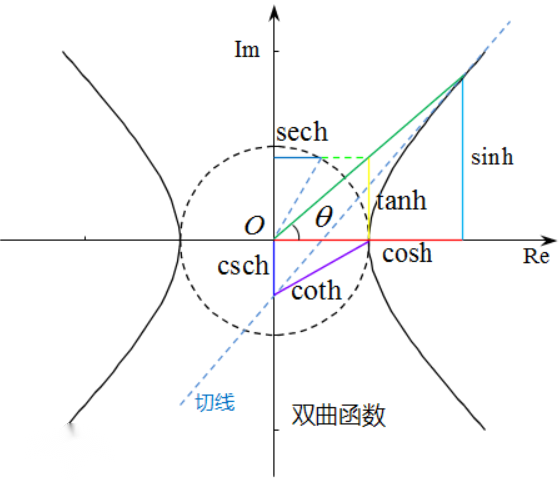
\includegraphics[width=9.5cm,height=8cm]{"figure/Summary/双曲函数.png"}
	\caption{双曲函数示意图}
	\label{Figure: 双曲函数示意图}
\end{figure} 
\begin{definition}\label{def: 双曲函数}
	双曲函数是一种类似于三角函数的一类函数,基本的函数有双曲正弦函数和双曲余弦函数,借由指数函数定义.
	
	1. 双曲正弦函数 
	$$\sinh x=\frac{e^{x}-e^{-x}}{2},x\in \mathbb{R}\quad \mathbb{R}\rightarrow \mathbb{R}$$
	
	2. 双曲余弦函数
	$$\cosh x=\frac{e^{x}+e^{-x}}{2},x\in \mathbb{R}\quad \mathbb{R}\rightarrow [1,+\infty]$$
	
	3. 双曲正切函数
	$$\tanh x=\frac{e^{x}-e^{-x}}{e^{x}+e^{-x}},x\in \mathbb{R}\quad \mathbb{R}\rightarrow (-1,1)$$
	
	恒等式:  
	$$\cosh^2 x-\sinh^2=1$$
	$$\sinh x=-i\sin ix,\quad \cosh x=\cos ix$$
	$$\sinh x=\sum\limits_{n=0}^{+\infty}\frac{x^{2n+1}}{(2n+1)!}=x+\frac{x^3}{3!}+\frac{x^5}{5!}+\dots$$
	$$\cosh x=\sum\limits_{n=0}^{+\infty}\frac{x^{2n}}{2n!}=1+\frac{x^2}{2!}+\frac{x^4}{4!}+\dots$$
\end{definition}
\begin{definition}
	反双曲函数:  
	
	1. 反双曲正弦函数
	$$\arsinh x=ln(x+\sqrt{x^2+1}),\quad (arsinh x)'=\frac{1}{\sqrt{x^2+1}}$$
	
	2. 反双曲余弦函数
	$$\arcosh x=ln(x+\sqrt{x^2-1}),\quad (arcosh x)'=\frac{1}{\sqrt{x^2-1}}$$
	
	3. 反双曲正切函数
	$$\artanh x=\frac{1}{2}ln(\frac{1+x}{1-x}),\quad (artanh x)'=\frac{1}{1-x^2}$$
\end{definition}


\section{特殊曲线}

\begin{definition}\label{def: 常用曲线}
	几类特殊曲线的面积、弧长、旋转体体积
	
	1.心形线 \quad $r=a(1+\cos \theta)$
	$$L=\int_{0}^{2\pi}\sqrt{a^2(1+\cos \theta)^2+a^2\sin^2\theta}d\theta=8a$$
	$$S=\int_{0}^{2\pi}a^2(1+\cos \theta)^2d\theta=3\pi a^2$$
	
	2.摆线\quad 
	$\left\lbrace
	\begin{array}{l}
		x=a(\theta-\sin \theta)\\
		y=a(1-\cos \theta)
	\end{array}
	 \right. $
	 $$L=\int_{0}^{2\pi}\sqrt{a^2(1-\cos \theta)^2+a^2\sin^2\theta}d\theta=8a$$
	 $$S=\int_{0}^{2a\pi}f(x)dx=\int_{0}^{2\pi}a^2(1-\cos \theta)^2d\theta=3\pi a^2$$
	
	3.星形线\quad $x^{\frac{2}{3}}+y^{\frac{2}{3}}=a^{\frac{2}{3}}\Leftrightarrow$
	$\left\lbrace
	\begin{array}{l}
		x=a\cos^3\theta\\
		y=a\sin^3\theta
	\end{array}
	 \right. $
	$$L=4\int_{0}^{\frac{\pi}{2}}3a\sin\theta\cos\theta d\theta=6a$$
	$$S=4\int_{0}^{\frac{\pi}{2}}3a\sin^4\theta\cos^2\theta=\frac{3\pi}{8}a^2$$
	
	4.三叶玫瑰线 \quad $\rho=a\cos 3\theta$\quad $\rho=a\sin 3\theta$
	$$L=6\int_{0}^{\frac{\pi}{6}}\sqrt{a^2\cos^2 3\theta+9a^2\sin^2 3\theta}d\theta=2a\int_{0}^{\frac{\pi}{2}}\sqrt{1+8\sin^2 t}dt$$
	$$S=3\int_{0}^{\frac{\pi}{6}}a^2\cos^2 3\theta d\theta=\frac{\pi a^2}{4}$$
	
	5.伯努利双扭线\quad $\rho^2=a^2\cos 2\theta$
	$$L=4\int_{0}^{\frac{\pi}{4}}a\sqrt{\frac{\sin^2 2\theta}{\cos 2\theta}+\cos^2 2\theta}d\theta=2a\int_{0}^{\frac{\pi}{2}}\sqrt{\dfrac{1-\cos^{2}\theta +\cos^{3}\theta}{\cos\theta}} d\theta$$
	$$S=2\int_{0}^{\frac{\pi}{4}}a^2\cos 2\theta d\theta=a^2$$
\end{definition}
\begin{figure}[H]
	\centering  %图片全局居中
	\subfigure[心形线]{
	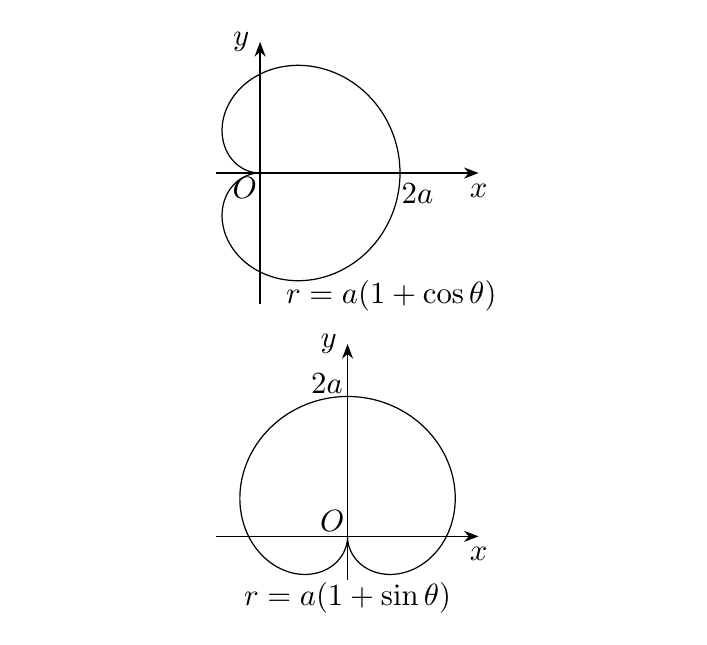
\includegraphics[width=0.45\textwidth]{"figure/Summary/心形线.png"}}
	\subfigure[摆线]{
	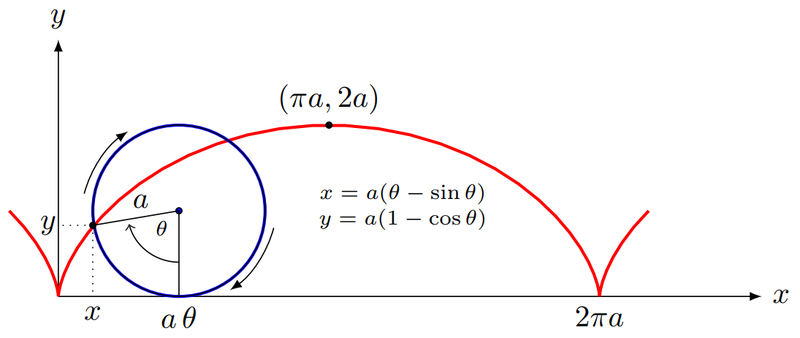
\includegraphics[width=0.45\textwidth]{"figure/Summary/摆线.png"}}
	\subfigure[星形线]{
	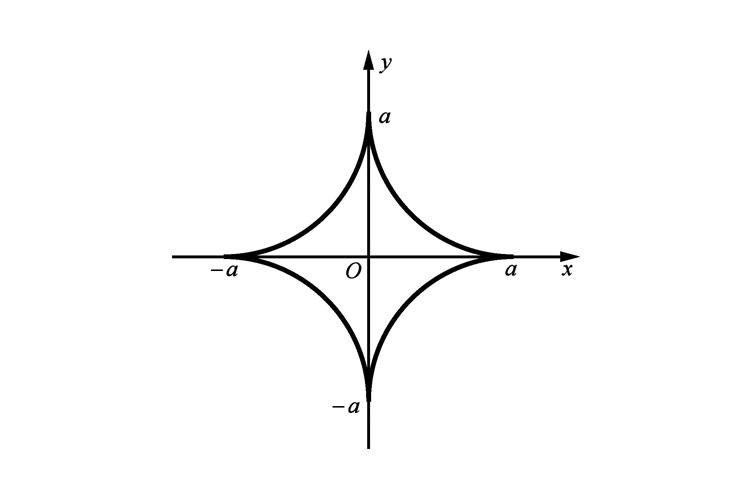
\includegraphics[width=0.45\textwidth]{"figure/Summary/星形线.jpg"}}
	\subfigure[三叶玫瑰线$\rho=a\cos 3\theta$]{
	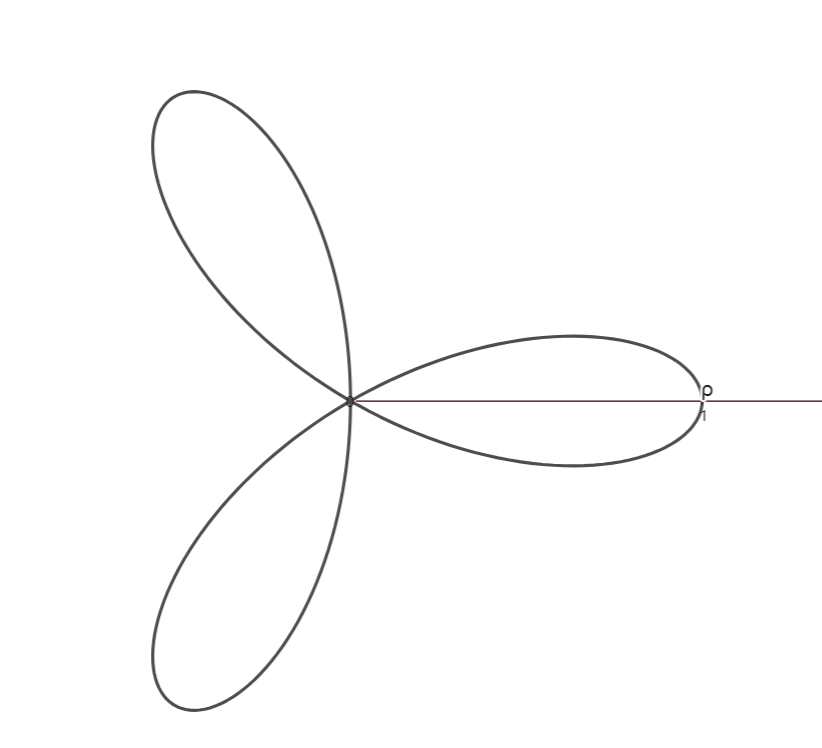
\includegraphics[width=0.45\textwidth]{"figure/Summary/三叶玫瑰线1.png"}}
	\subfigure[三叶玫瑰线$\rho=a\sin 3\theta$]{
	
\includegraphics[width=0.45\textwidth]{"figure/Summary/三叶玫瑰线2.png"}}
	\subfigure[伯努利双扭线$\rho^2=a^2\cos 2\theta$]{
	
\includegraphics[width=0.45\textwidth]{"figure/Summary/伯努利双扭线.png"}}
	\caption{曲线图形}
\end{figure}

\section{两类欧拉积分}

\begin{definition}[$Gamma$ 函数和 $Beta$函数]	
	1. $Gamma$ 函数(欧拉第一类积分)
	$$B(p,q)=\int_{0}^{1}x^{p-1}(1-x)^{q-1}dx=B(q,p)$$
	
	我们有:  $$B(a,b)=(\frac{x^a(1-x)^b}{a})|_{0}^{1}+\frac{b-1}{a}\int_{0}^{1}x^{a}(1-x)^{b-2}dx$$
	$$B(a,b)=\frac{b-1}{a}\int_{0}^{1}(x-1+1)x^{a-1}(1-x)^{b-2}$$
	$$\mathcolorbox{yellow}{B(a,b)=\frac{b-1}{a}[B(a,b-1)-B(a,b)]}$$ $$\mathcolorbox{yellow}{B(a,b)=\frac{b-1}{a+b-1}B(a,b-1)}$$
	
	特别的,我们有:  $$\mathcolorbox{yellow}{B(m,n)=\frac{(n-1)!(m-1)!}{(m+n-1)!}}$$
	
	2.$Beta$函数(第二类欧拉积分)
	$$\Gamma(\alpha)\begin{cases} \int_{0}^{+\infty}x^{\alpha-1}e^{-x}dx\\ 2\int_{0}^{+\infty}x^{2\alpha-1}e^{-x^{2}}dx \end{cases}$$
	
	我们有:  $$\Gamma(\alpha)=(-x^{\alpha-1}e^{-x})|_{0}^{+\infty}+(\alpha-1)\int_{0}^{+\infty}x^{\alpha-2}e^{-x}dx$$
	$$\mathcolorbox{red}{\Gamma(\alpha)=(\alpha-1)\Gamma(\alpha-1)},\alpha>1$$

	有两个特别的 $\alpha$, 分别是 $\alpha = \dfrac{1}{2}$ 和 $\alpha = 1$:

	$$\begin{cases} \int_{0}^{+\infty}e^{-x}dx = 1, & \alpha =1 \\ 
		\int_{0}^{+\infty}x^{-\frac{1}{2}}e^{-x}dx = 2\int_{0}^{+\infty}e^{-x^{2}}dx = \sqrt{\pi}, & \alpha =\dfrac{1}{2}\end{cases}$$
	
	特别的,我们有:  $$\mathcolorbox{red}{\Gamma(n+1)=n!}$$
	
	3. 两类积分之间的关系
	
	转换公式:  
	$$B(a,b)=\frac{\Gamma(a)\Gamma(b)}{\Gamma(a+b)}$$
	
\end{definition}


\section{谱分解定理}

\begin{definition}[代数重复度]
	设$\lambda_{1},\lambda_{2},\cdots,\lambda_{k}$是矩阵$A\in \mathbb{C}^{n\times n}$的相异特征值,其重数分别为$r_{1},r_{2},\cdots,r_{k}$,称$r_{i}$为矩阵$A$的特征值$\lambda_{i}$的代数重复度.
\end{definition}
\begin{definition}[几何重复度]
	齐次方程组$Ax=\lambda_{i}x\ (i=1,2,\cdots,k)$的解空间$V_{\lambda_{i}}$称为$A$的对应于特征值$\lambda_{i}$的特征空间,则$V_{\lambda_{i}}$的维数称为$A$的特征值$\lambda_{i}$的几何重复度.
\end{definition}
\begin{definition}[单纯矩阵]
	若矩阵$A$的每一个特征值的代数重复度与几何重复度相等,则称矩阵$A$为单纯矩阵.
\end{definition}
\begin{definition}[幂等矩阵]
	若$A$为方阵,且$A^2=A$,则称$A$为幂等矩阵.
\end{definition}
\begin{property}[幂等矩阵$A$性质]
	\begin{itemize}
		\item (1). $A$是单纯矩阵,且其$Jordan$标准型为$\left(\begin{matrix}
			I_{r}&0\\0&0
		\end{matrix} \right) $
		\item (2). $A$的特征值只能为$0$或者$1$
		\item (3). $rank(A)=tr(A)$
		\item (4). $Ax=x\Leftrightarrow x\in\mathbb{R}(A)$
		\item (5). $A$一定可以相似对角化
	\end{itemize}
\end{property}
\begin{theorem}[谱分解定理]\label{the: 谱分解定理}
	设$A\in\mathbb{C}^{n\times n}$是单纯矩阵,矩阵$A$有$k$个相异特征值$\lambda_{i}\ (i=1,2,\cdots,k)$,$\exists A_{i}\in \mathbb{C}^{n\times n}\ (i=1,2,\cdots,k)$,使得
	$$A=\sum\limits_{i=1}^{k}\lambda_{i}G_{i}$$
	
	此式称为矩阵$A$的谱分解,$G_{1},G_{2},\cdots,G_{k}$称为$A$的族谱,且满足一下性质:  
	\begin{property}[谱分解谱族$G_{i}$性质]
		\begin{itemize}
			\item (1). 幂等性:  $G_{i}^2=G_{i}$
			\item (2). 分离性:  $G_{i}G_{j}=0\ (i\neq j)$
			\item (3). 可加性:  $\sum\limits_{i=1}^{k}G_{i}=E_{n}$
		\end{itemize}
	\end{property}
	\begin{corollary}[谱族$G_{i}$推论]
		\begin{itemize}
			\item $AG_{i}=G_{i}A=\lambda_{i}G_{i}$
			\item $rank(G_{i})=m_{i}$
			\item $G_{i}$是唯一的,$G$的族谱是唯一的.
		\end{itemize}
	\end{corollary}
	\begin{proposition}
		矩阵$A$是单纯矩阵等价为存在$k$个矩阵$G_{i},\ (i=1,2,\cdots,k)$满足:  
		\begin{itemize}
			\item (1). $G_{i}G_{j}=\left\lbrace
			\begin{array}{l}
				G_{i},\ i=j\\0,\ i\neq j
			\end{array}
			\right. $
			\item (2). $\sum\limits_{i=1}^{k}G_{i}=E_{n}$
			\item (3). $A=\sum\limits_{i=1}^{k}\lambda_{i}G_{i}$
			\item (4). $f(A)$为任意多项式,则$$f(A)=\sum\limits_{i=1}^{k}f(\lambda_{i})G_{i}$$
			\item (5). $A^m=\sum\limits_{i=1}^{k}\lambda_{i}^mG_{i}$
		\end{itemize}
	\end{proposition}
\end{theorem}
\begin{anymark}[证明]
	1. 必要性
	 
	(1). 当$k=n$时:  
	
	我们由$A$是单纯矩阵可以得到矩阵$A$可以相似对角化
	$$A=P\Lambda P^{-1},\text{其中}\Lambda=diag\{\lambda_{1},\lambda_{2},\cdots,\lambda_{n}\}$$
	
	我们不妨设$P=(v_{1},v_{2},\cdots,v_{n})$,$P^{-1}=\left( \begin{matrix}
		\omega_{1}^{T}\\\omega_{2}^{T}\\ \vdots\\\omega_{n}^{T}
	\end{matrix}\right) $,我们可以得到:  
	$$A=(v_{1},v_{2},\cdots,v_{n})\left[\begin{matrix}
		\lambda_{1}&0&\cdots&0\\
		0&\lambda_{2}&\cdots&0\\
		\cdots&\cdots&\cdots&\cdots\\
		0&0&\cdots&\lambda_{n}
	\end{matrix} \right] \left( \begin{matrix}
		\omega_{1}^{T}\\\omega_{2}^{T}\\ \vdots\\\omega_{n}^{T}
	\end{matrix}\right) \Rightarrow A=\sum\limits_{i=1}^{n}\lambda_{i}v_{i}\omega_{i}^{T}=\sum\limits_{i=1}^{n}\lambda_{i}G_{i},\ \text{其中}G_{i}=v_{i}\omega_{i}^{T}$$
	
	我们由$\left\lbrace
	\begin{array}{l}
		P^{-1}P=E_{n}\\
		PP^{-1}=E_{n}
	\end{array}
	\right.\Rightarrow\left\lbrace
	\begin{array}{l}
		\omega_{i}^{T}v_{j}=\left\lbrace
		\begin{array}{l}
			1,\ i=j\\
			0,\ i\neq j
		\end{array}
		\right. \\
		\sum\limits_{i=1}^{n}v_{i}\omega_{i}^{T}=\sum\limits_{i=1}^{n}G_{i}=E_{n}
	\end{array}
	\right.$
	
	对于任意$i,j\in(1,n),G_{i}G_{j}=v_{i}(\omega_{i}^{T}v_{j})\omega_{j}^{T}$,我们可以得到:  
	$$G_{i}G_{j}=\left\lbrace
	\begin{array}{l}
		v_{i}\omega_{i}^{T}=G_{i},\ i=j\\
		0,\ i\neq j
	\end{array}
	\right. \Rightarrow A_{i}\text{是幂等矩阵}$$
	
	(2). 当$k<n$时:  
	
	我们由矩阵$A$是单纯矩阵,可以得到:  $A=P\Lambda P^{-1}$
	$$\left\lbrace
	\begin{array}{l}
		P=(v_{11},v_{12},\cdots,v_{1r_{1}},v_{21},v_{22},\cdots,v_{2r_{2}},\cdots,v_{k1},v_{k2},\cdots,v_{kr_{k}})\\
		P^{-1}=(\omega_{11}^{T},\omega_{12}^{T},\cdots,\omega_{1r_{1}}^{T},\omega_{21}^{T},\omega_{22}^{T},\cdots,\omega_{2r_{2}}^{T},\cdots,\omega_{k1}^{T},\omega_{k2}^{T},\cdots,\omega_{kr_{k}}^{T})^{T}
	\end{array}
	\right. $$
	$$A=\sum\limits_{i=1}^{k}\lambda_{i}\sum\limits_{j=1}^{r_{i}}B_{ij}\stackrel{G_{i}=\sum\limits_{j=1}^{r_{i}}B_{ij}}{\longrightarrow}A=\sum\limits_{i=1}^{k}\lambda_{i}G_{i}$$
	$$P^{-1}P=E_{n}\Rightarrow \omega_{ij}^{T}v_{lk}=\left\lbrace
	\begin{array}{l}
		1,\ i=l,j=k\\
		0,\ i\neq l\text{或}j\neq k
	\end{array}
	\right. $$
	$$B_{ij}B_{lk}=v_{ij}(\omega_{ij}^{T}v_{lk})\omega_{lk}^{T}=\left\lbrace
	\begin{array}{l}
		B_{ij},\ i=l,j=k\\
		0,\ i\neq l\text{或}j\neq k
	\end{array}
	\right. \Rightarrow G_{i}G_{j}=\sum\limits_{p=1}^{r_{i}}B_{ip}\sum\limits_{q=1}^{r_{j}}B_{jq}=\left\lbrace
	\begin{array}{l}
		G_{i},\ i=j\\0,\ i\neq j
	\end{array}
	\right. $$
	$$\sum\limits_{i=1}^{k}G_{i}=\sum\limits_{i=1}^{n}B_{i}=E_{n}$$
	(2). 充分性
	
	我们首先可以得到矩阵$G_{i}$均为幂等矩阵,我们不妨设$dim\mathbb{R}(G_{i})=n_{i}$,我们可以得到:  
	$$n_{i}=tr(G_{i})\Rightarrow \sum\limits_{i=1}^{k}n_{i}=\sum\limits_{i=1}^{k}tr(G_{i})=tr(\sum\limits_{i=1}^{k}G_{i})=tr(E_{n})=n$$
	
	我们取$X_{i}$为$\mathbb{R}(G_{i})$的基列构成的阵,则$X=(X_{1},X_{2},\cdots,X_{k})$是$n\times n$矩阵,且$G_{i}$的列向量都可以由$X_{i}$线性表出,我们可以得到:  
	$$G_{i}=(X_{i}\beta_{1},X_{i}\beta_{2},\cdots,X_{i}\beta_{n})=X_{i}Y_{i}$$
	$$XY=(X_{1},X_{2},\cdots,X_{n})\left( \begin{matrix}
		Y_{1}\\Y_{2}\\\vdots\\Y_{n}
	\end{matrix}\right)=\sum\limits_{i=1}^{n}X_{i}Y_{i}=E_{n}\Rightarrow \text{矩阵}X\text{可逆}$$

	$$YX=\left( \begin{matrix}
		Y_{1}\\Y_{2}\\\vdots\\Y_{n}
	\end{matrix}\right)(X_{1},X_{2},\cdots,X_{k})=\left[ \begin{matrix}
	Y_{1}\\Y_{2}\\\cdots\\Y_{k}
\end{matrix}\right] =\left[\begin{matrix}
Y_{1}X_{1}&Y_{1}X_{2}&\cdots&Y_{1}X_{k}\\
Y_{2}X_{1}&Y_{2}X_{2}&\cdots&Y_{2}X_{k}\\
\cdots&\cdots&\cdots&\cdots\\
Y_{k}X_{1}&Y_{k}X_{2}&\cdots&Y_{k}X_{k}\\
\end{matrix} \right] =E_{n}=\left[\begin{matrix}
E_{r_{1}}&0&\cdots&0\\
0&E_{r_{2}}&\cdots&0\\
\cdots&\cdots&\cdots&\cdots\\
0&0&\cdots&E_{r_{k}}\\
\end{matrix} \right]$$

我们可以得到:  
$$Y_{i}X_{j}=\left\lbrace
\begin{array}{l}
	E_{r_{i}},\ i=j\\
	0,\ i\neq j
\end{array}
\right. \Rightarrow G_{i}X_{j}=x_{i}Y_{i}X_{j}=\left\lbrace
\begin{array}{l}
	X_{i},\ i=j\\
	0,\ i\neq j
\end{array}
\right. $$

	我们利用幂等矩阵的性质
	\begin{eqnarray*}
		AX&=&(\sum\limits_{i=1}^{k}\lambda_{i}G_{i})(X_{1},X_{2},\cdots,X_{k})\\
		&=&((\sum\limits_{i=1}^{k}\lambda_{i}G_{i})X_{1},(\sum\limits_{i=1}^{k}\lambda_{i}G_{i})X_{2},\cdots,(\sum\limits_{i=1}^{k}\lambda_{i}G_{i})X_{k})\\
		&=&(\lambda_{1}X_{1},\lambda_{2}X_{2},\cdots,\lambda_{k}X_{k})\\
		&=&(X_{1},X_{2},\cdots,X_{k})\left[\begin{matrix}
			E_{r_{1}}&0&\cdots&0\\
			0&E_{r_{2}}&\cdots&0\\
			\cdots&\cdots&\cdots&\cdots\\
			0&0&\cdots&E_{r_{k}}\\
		\end{matrix} \right]\\
	&=&X\Lambda\Rightarrow A=X\Lambda X^{-1} 
	\end{eqnarray*}
	
	(3). 谱分解唯一性
	
	我们不妨假设$F_{1},F_{2},\cdots,F_{k}$满足:  
	$$\left\lbrace
	\begin{array}{l}
		F_{i}F_{j}=0,\ i\neq j\\
		F_{i}^2=F_{i}\\
		A=\sum\limits_{i=1}^{k}\lambda_{i}F_{i}\\
		\sum\limits_{i=1}^{k}F_{i}=E_{n}
	\end{array}
	\right. $$
	
	我们由族谱$G_{i}$性质推论可以得到:  
	$$\left\lbrace
	\begin{array}{l}
		AG_{i}=G_{i}A=\lambda_{i}G_{i}\\
		AF_{i}=F_{i}A=\lambda_{i}F_{i}
	\end{array}
	\right. \Rightarrow \left\lbrace
	\begin{array}{l}
		AG_{i}F_{j}=\lambda_{i}G_{i}F_{j}\\
		\lambda_{i}G_{i}F_{j}=G_{i}AF_{j}\\
		G_{i}AF_{j}=\lambda_{j}G_{i}F_{j}
	\end{array}
	\right. \Rightarrow G_{i}F_{j}=0,\ i\neq j$$
	
	我们得到:  $$G_{i}=G_{i}E_{n}=G_{i}(\sum\limits_{j=1}^{k}F_{j})=G_{i}F_{i}=(\sum\limits_{j=1}^{k}G_{j})F_{i}=F_{i}$$
	
	综上所述,矩阵$A$的谱分解是唯一的.
\end{anymark}
\myspace{1}


\section{多项式函数极值点和拐点}


\begin{theorem}[代数基本定理]\label{the: 代数基本定理}
	任何一个一元 $n$ 次复系数多项式, 都恰好有 $n$ 个复根, 且可以表示为 $n$ 个一次因式的乘积.
\end{theorem}

\begin{corollary}[曲线的极值点和拐点]
	曲线上的可导点不可能同时是极值点和拐点, 不可导点可能同时是极值点和拐点.
\end{corollary}

\begin{proposition}[多项式函数极值点和拐点个数:命题一]\label{pro: 命题一}
	多项式函数 $f(x) = (x-a)^{n},(n>1)$, 当 $n$ 为奇数时, $(a,0)$ 是 $f(x)$ 的拐点, 当 $n$ 为偶数时, $x=a$ 是 $f(x)$ 的极值点.
\end{proposition}
\begin{anymark}[证明]

	$$f'(x) = n(x-a)^{n-1},\quad f''(x) = n(n-1)(x-a)^{n-2}$$
	当 $n$ 为偶数时, 我们有: $f'(a) = 0$ 且 
	$$\exists x\in \mathring{U}(a,\delta), f(x) = (x-a)^{n} > 0 = f(a)$$

	或者 
	$$\exists \delta > 0, x\in (a-\delta,a),f'(x)<0; x\in (a,a+\delta),f'(x)>0$$
	
	我们有: 当 $n$ 为偶数时, $x=a$ 是 $f(x)$ 的极值点.
	
	当 $n$ 为奇数时, 我们有: $f''(a) = 0$ 且
	
	$$\exists \delta > 0, x\in (a-\delta,a),f''(x)<0; x\in (a,a+\delta),f''(x)>0$$

	我们有: 当 $n$ 为奇数时, $(a,0)$ 是 $f(x)$ 的拐点.
	

\end{anymark}


\begin{proposition}[多项式函数极值点和拐点个数:命题二]\label{pro: 命题二}
	多项式函数 $f(x) = (x-a)^{n}g(x), (n>1), g(a)\neq 0$, 当 $n$ 为奇数时, $(a,0)$ 是 $f(x)$ 的拐点, 当 $n$ 为偶数时, $x=a$ 是 $f(x)$ 的极值点.
\end{proposition}
\begin{anymark}[证明]

	$$\begin{cases}
		f'(x) = ng(x)(x-a)^{n-1} + g'(x)(x-a)^{n} = (x-a)^{n-1}[ng(x)+(x-a)g'(x)]\\
		f''(x) = (x-a)^{n-2}[n(n-1)g(x) +2n(x-a)g'(x)+(x-a)^{2}g''(x)]
	\end{cases}$$

	当 $n$ 为偶数时, 我们不妨假设 $g(a) > 0$, 根据极限的保号性,我们有:
	$$\exists \delta_{1} > 0, s.t.\ x\in U(a,\delta_{1}), g(a) > 0$$
	
	当 $x\in U(a,\delta_{1}), f(x) = (x-a)^{n}g(x) \geq f(a) =0$, $x=a$ 是 $f(x)$ 的一个极值点. 


	当 $n$ 为奇数时, $x\to a,(x-a),(x-a)^{2}$都是无穷小量, $g'(a),g''(a)$ 都是定值, 因此
	$$\exists \delta_{2} > 0, s.t.\ x\in U(a,\delta_{2}), 2n(x-a)g'(x)+(x-a)^{2}g''(x)\leq |n(n-1)g(x)| $$

	我们有: $x\in U(a,\delta_{2}), [n(n-1)g(x) +2n(x-a)g'(x)+(x-a)^{2}g''(x)] > 0$, 即: $f''(x)$ 与 $(x-a)^{n-2}$ 符号相同

	当 $x\in (a-\delta_{2},a), f''(x) < 0; x\in (a,a+\delta_{2}), f''(x) > 0$, $(a,0)$ 是 $f(x)$ 的一个拐点.
\end{anymark}

\begin{proposition}[多项式函数极值点和拐点个数:命题三]\label{pro: 命题三}
	讨论多项式函数: $P_{n}(x) = \prod\limits_{i=1}^{k}(x-a_{i})^{p_{i}}$ 极值点和拐点个数,其中满足:
	$$a_{i}\in\mathbb{R}, a_{1}<a_{2}<\cdots<a_{k}, p_{i}\in \mathbb{Z}^{+}$$
\end{proposition}

\begin{anymark}[证明]
	我们首先有: $P_{n}(x)$ 是多项式函数, 在 $\mathbb{R}$ 上 $n$ 阶可导, $P_{n}(x)$ 的极值点一定满足: $P_{n}'(x) = 0$, 拐点满足: $P_{n}''(x) = 0$
	\myspace{1}

	$P(x)$ 有 $k$ 个实数根, 这 $k$ 个实数根的重数分别为: $p_{1},p_{2},\cdots,p_{k}$, 且 $\sum\limits_{i=1}^{k}p_{i}= n$

	我们利用多个函数连乘的求导公式:
	$$P_{n}'(x) =  \prod\limits_{i=1}^{k}(x-a_{i})^{p_{i}-1}\left[\sum\limits_{i=1}^{k}p_{i}\left(\prod\limits_{j=1\\j\neq i}^{k}(x-a_{j})\right)\right]$$

	当 $p_{i} \geq 2 (i = 1,2,\cdots,k)$ 时, $x=a_{i}(i=1,2,\cdots,k)$ 是 $P_{n}'(x)$ 的一个零点,此类的驻点一共有 $k$ 个, $P_{n}'(x)$ 有 $p_{i}-1 (i=1,2,\cdots,k)$ 重根 $a_{i}(i=1,2,\cdots,k)$
	\myspace{1}
	$P_{n}'(x)$ 此类的零点个数为: $n_{1} = \sum\limits_{i=1}^{k}(p_{i}-1) = n-k$
	\myspace{1}
	在 $(a_{i},a_{i+1}),(i=1,2,\cdots,k-1)$ 中, 我们由罗尔定理得到: $\exists \xi_{i}\in(a_{i},a_{i+1}),(i=1,2,\cdots,k-1), s.t.\ P'(\xi_{i}) = 0$, 此类零点的个数为 $k-1$ 个
	\myspace{1}
	$P'_{n}(x)$ 是 $n-1$ 次多项式函数, 至多有 $n-1$ 个复根, 我们得到 $P'_{n}(x)$ 有 $n-k+k-1 = n-1$ 个实数根, 其中前面 $n-k$ 个根中存在重根情况.
	\begin{corollary}[多项式函数零点]
		$P_{n}(x)$ 有 $n$ 个实数根(含重根), 那么 $P_{n}'(x),P_{n}''(x),\cdots,P_{n}^{(n-1)}(x)$ 的根全部是实数.
	\end{corollary}

	我们继续看 $P_{n}'(x)$ 的两类零点, 其中一类是 $x=a_{i}(i=1,2,\cdots,k),(p_{i}>1)$, 另一类是 $x=\xi_{i}(i=1,2,\cdots,k-1)$
	\myspace{1}
	第一类零点:我们由 $\mathbf{pro: }$ \ref{pro: 命题二}得到: 当 $p_{i}$ 为偶数的时候, $a_{i}$ 是 $P_{n}(x)$ 的极值点, 当 $p_{i}$ 为奇数的时候, $a_{i}$ 是 $P_{n}(x)$ 的拐点
	\myspace{1}
	第二类零点: $P_{n}'(x) = \sum\limits_{i=1}^{n-1}(x-\eta_{i}),\eta_{i}\in\mathbb{R}$, 当 $x\in U(\xi_{i},\delta)$ 时, 只有 $(x-\xi_{i})$ 这一项符号改变, 因此 $x=\xi_{i}$ 是 $P_{n}(x)$ 极值点
	\myspace{1}
	我们不妨假设 $p_{i} > 1\ \&\ p_{i}\text{为奇数}$ 的个数为 $k_{1}$, $p_{i} > 1\ \&\ p_{i}\text{为偶数}$ 的个数为 $k_{2}$
	\myspace{1}
	$P_{n}(x)$ 的极值点个数为 $k-1+k_{2}$

	\myspace{2}
	关于拐点的个数,我们可以类比极值点个数的方法, 将 $P_{n}'(x)$ 当做原函数,求 $P_{n}'(x)$ 的极值点个数, 我们将 $P_{n}'(x)$改写为:
	
	$$P_{n}'(x) = \sum\limits_{i=1}^{k}p_{i}\left[(x-a_{1})^{p_{1}-1}(x-\xi_{1})(x-a_{2})^{p_{2}-1}\cdots(x-\xi_{k-1})(x-a_{k})^{p_{k}-1}\right]$$

	我们得到:
	\myspace{1}
	1. $P_{n}'(x)$ 有零点 $a_{1},\xi_{1},a_{2},\cdots,a_{k-1},\xi_{k-1},a_{k}$, 其中 $a_{i}$ 是重根, $\xi_{i}$ 是非重根
	\myspace{1}
	2. 根据罗尔定理, 我们得到: 在 $P_{n}'(x)$ 每两个零点之间存在 $\eta_{j}$, 使得 $P_{n}''(x) = 0$, 且是 $P_{n}''(x)$ 的极值点, 也是 $P_{n}(x)$ 的拐点, 个数为: $k_{1}+k_{2}+k-2$
	\myspace{1}
	3. $a_{i}(i=1,2,\cdots,k)$ 中, 满足 $p_{i} > 1$ 且 $p_{i}-1$ 为偶数, 也就是 $p_{i}$ 为奇数时, $x = a_{i}$ 是 $P_{n}''(x)$ 的极值点, 也是 $P_{n}(x)$ 的拐点, 个数为: $k_{1}$
	\myspace{1}
	4. $P_{n}(x)$ 的拐点个数: $k+2k_{1}+k_{2}-2$
	\myspace{1}
	综上所述, 我们有以下的结论:
	\begin{corollary}[极值点和拐点个数]
		假设 $P_{n}(x)=\prod\limits_{i=1}^{k}(x-a_{i})^{p_{i}}$, 其中 $k_{1}$ 个 $p_{i}$ 为奇数(大于 $1$), $k_{2}$ 个 $p_{i}$ 为偶数, $k_{0}$ 个 $p_{i}=1$, 满足 $k_{0}+k_{1}+k_{2} = k$, 我们有:
		\begin{itemize}
			\item $P_{n}(x)$ 的极值点个数: $k-1+k_{2} = k_{0}+k_{1}+2k_{2}-1$
			\item $P_{n}(x)$ 的拐点个数: $k+2k_{1}+k_{2}-2 = k_{0}+3k_{1}+2k_{2}-2$
		\end{itemize}
	\end{corollary}
\end{anymark}

\section{柯西收敛准则}

\begin{theorem}[柯西收敛准则]\label{the: 柯西收敛准则}
	柯西极限存在准则, 又称柯西收敛准则, 给出某个式子(数列、数项级数、函数等)收敛的一个充分必要条件, 主要应用在数列、数项级数、函数、反常积分、函数列和函数项级数等的收敛性判断中.
\end{theorem}

\begin{proposition}[柯西收敛准则:数列]
	数列 $\{a_{n}\}$ 收敛的充分必要条件是: 对于任意 $\varepsilon > 0$, 存在 $N\in\mathbb{N}$, 当 $n,m>N$ 时, $|a_{n}-a_{m}|<\varepsilon$, 我们将满足条件的 $\{a_{n}\}$ 称为柯西序列, 上述定理也可表述为: 数列 $\{a_{n}\}$ 收敛当且仅当 $\{a_{n}\}$ 是柯西序列
\end{proposition}

\begin{anymark}[证明]
	(1). 必要性:

	不妨设 $\lim\limits_{n\to \infty} a_{n} =\eta$, 对于任意 $\varepsilon > 0$, 存在 $N_{0}\in\mathbb{N}$, 当 $n>N_{0}$ 时, $|a_{n}-\eta|<\dfrac{\varepsilon}{2}$, 我们有:
	$$\begin{cases} 
		\forall n > N_{0}, s.t.\ |a_{n} - \eta| < \dfrac{\varepsilon}{2}\\ 
		\forall m > N_{0}, s.t.\ |a_{m} - \eta| < \dfrac{\varepsilon}{2}
	\end{cases}
	\Rightarrow 
	|x{n}-x_{m}| = |(x_{n} - \eta) - (x_{m} - \eta)| \leq |x_{n} - \eta| + |x_{m}-\eta| \leq \varepsilon$$

	(2). 充分性:


\end{anymark}

\begin{proposition}[柯西收敛准则:数项级数]
	
\end{proposition}

\begin{anymark}[证明]
	(1). 必要性:

	不妨设 $\lim\limits_{n\to \infty} a_{n} =\eta$, 对于任意 $\varepsilon > 0$, 存在 $N_{0}\in\mathbb{N}$, 当 $n>N_{0}$ 时, $|a_{n}-\eta|<\dfrac{\varepsilon}{2}$, 我们有:
	$$\begin{cases} 
		\forall n > N_{0}, s.t.\ |a_{n} - \eta| < \dfrac{\varepsilon}{2}\\ 
		\forall m > N_{0}, s.t.\ |a_{m} - \eta| < \dfrac{\varepsilon}{2}
	\end{cases}
	\Rightarrow 
	|x_{n}-x_{m}| = |(x_{n} - \eta) - (x_{m} - \eta)| \leq |x_{n} - \eta| + |x_{m}-\eta| \leq \varepsilon$$

	(2). 充分性:


\end{anymark}

\begin{proposition}[柯西收敛准则:函数]
	
\end{proposition}
\section{阿达玛不等式}

\begin{figure}[htbp]
	\centering
	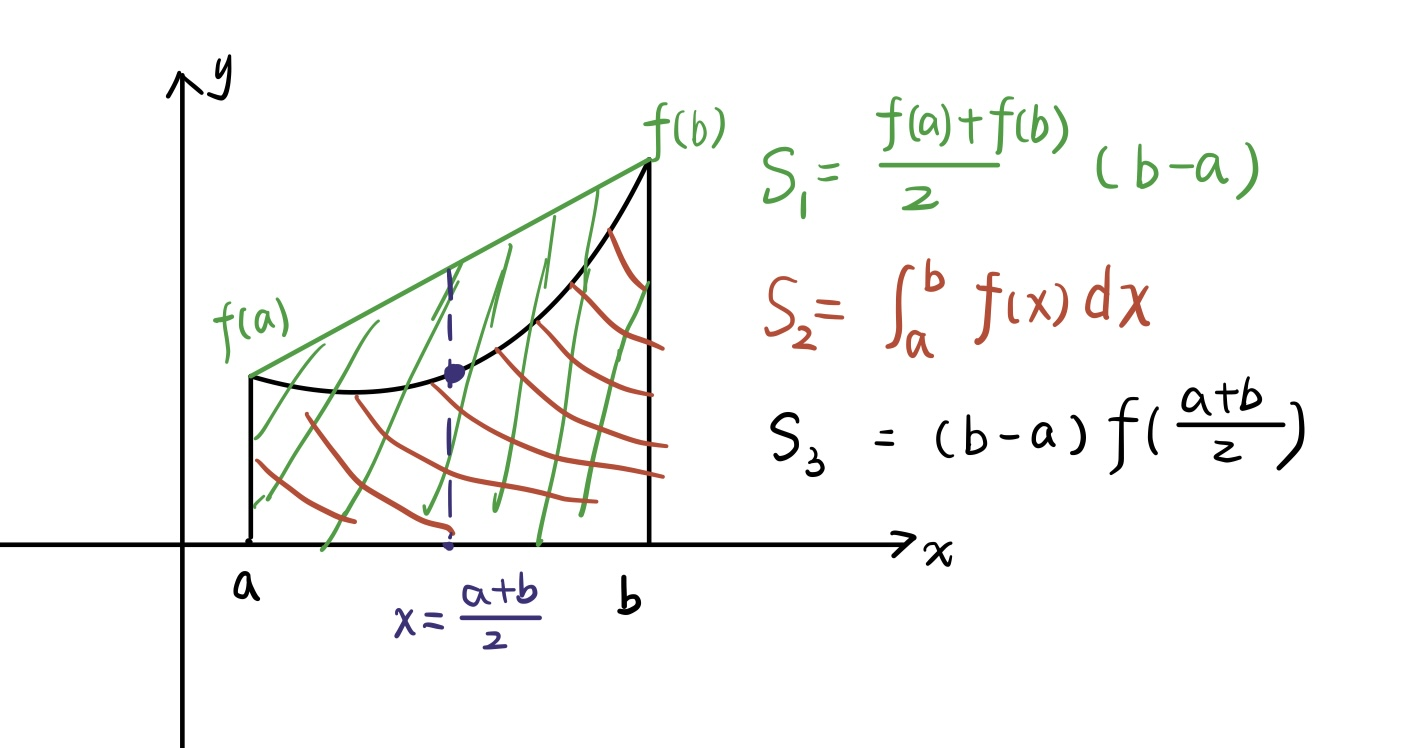
\includegraphics[width=15cm,height=8cm]{"figure/Summary/阿达玛不等式.jpg"}
	\caption{$Hadamard$不等式}
	\label{Figure: 阿达玛不等式}
\end{figure}

\begin{theorem}[$\mathbf{Hadamard}$不等式]\label{thm: 阿达玛不等式}

	$f(x)$在$[a,b]$上具有二阶导数,且$f''(x)\geq 0$,下面不等式成立:  
	$$f(\dfrac{a+b}{2})\leq \dfrac{1}{b-a}\int_{a}^{b}f(t)dt\leq \dfrac{1}{2}[f(a)+f(b)]$$
	\begin{proof}
		
		原不等式可以化为:  
		$$(b-a)f(\dfrac{a+b}{2})\leq\int_{a}^{b}f(t)dt\leq\dfrac{b-a}{2}[f(a)+f(b)]$$
		
		我们由图\ref{Figure: 阿达玛不等式}可以发现:  
		
		不等式左边表示的过$(\dfrac{a+b}{2},f(\dfrac{a+b}{2}))$的切线与$x=a,x=b,y=0$围成的图形的面积$S_{3}$;
		
		不等式中间表示的是$f(x)$与$x=a,x=b,y=0$围成的曲边梯形的面积$S_{2}$;
		
		不等式右边表示的是直线$x=a,x=b,y=0$与直线$y=\dfrac{f(b)-f(a)}{b-a}(x-a)+f(a)$围成的梯形的面积$S_{1}$.
		
		我们可以由图形上直观的看出三个面积的大小关系:  $S_{3}\leq S_{2}\leq S_{1}$
		
		对于左边的不等式,我们将$f(x)$在$x=\dfrac{a+b}{2}$处展开得到:  
		$$f(x)=f(\dfrac{a+b}{2})+f'(\dfrac{a+b}{2})(x-\dfrac{a+b}{2})+f''(\xi)(x-\dfrac{a+b}{2})^2$$
		
		我们由$f''(x)>0$,我们可以得到:  
		$$f(x)>f(\dfrac{a+b}{2})+f'(\dfrac{a+b}{2})(x-\dfrac{a+b}{2})$$
		
		两边同时在$[a,b]$内取定积分得到:  
		$$\int_{a}^{b}f(x)dx>\int_{a}^{b}[f(\dfrac{a+b}{2})+f'(\dfrac{a+b}{2})(x-\dfrac{a+b}{2})]=(b-a)f(\dfrac{a+b}{2})$$
		
		对于右边的不等式,我们构造辅助函数:  
		$$F(x)=\dfrac{x-a}{2}[f(x)+f(a)]-\int_{a}^{x}f(t)dt,\ F(a)=0$$
		$$\left\lbrace
		\begin{array}{l}
			F'(x)=\dfrac{x-a}{2}f'(x)-\dfrac{f(x)-f(a)}{2}\\
			F''(x)=\dfrac{x-a}{2}f''(x)
		\end{array}
		\right. F'(0)=0,F''(x)\geq 0\Rightarrow F'(x)\geq 0$$
		
		我们得到$F'(x)\geq 0\Rightarrow F(x)\text{单调递增}$,$F(x)\geq F(a)=0$
	\end{proof}
\end{theorem}

\end{document}